% Options for packages loaded elsewhere
\PassOptionsToPackage{unicode}{hyperref}
\PassOptionsToPackage{hyphens}{url}
\PassOptionsToPackage{dvipsnames,svgnames,x11names}{xcolor}
%
\documentclass[
  a4paper,
  pandoc,
  ja=standard,
  jafont=haranoaji]{bxjsbook}
\usepackage{amsmath,amssymb}
\usepackage{lmodern}
\usepackage{iftex}
\ifPDFTeX
  \usepackage[T1]{fontenc}
  \usepackage[utf8]{inputenc}
  \usepackage{textcomp} % provide euro and other symbols
\else % if luatex or xetex
  \usepackage{unicode-math}
  \defaultfontfeatures{Scale=MatchLowercase}
  \defaultfontfeatures[\rmfamily]{Ligatures=TeX,Scale=1}
\fi
% Use upquote if available, for straight quotes in verbatim environments
\IfFileExists{upquote.sty}{\usepackage{upquote}}{}
\IfFileExists{microtype.sty}{% use microtype if available
  \usepackage[]{microtype}
  \UseMicrotypeSet[protrusion]{basicmath} % disable protrusion for tt fonts
}{}
\makeatletter
\@ifundefined{KOMAClassName}{% if non-KOMA class
  \IfFileExists{parskip.sty}{%
    \usepackage{parskip}
  }{% else
    \setlength{\parindent}{0pt}
    \setlength{\parskip}{6pt plus 2pt minus 1pt}}
}{% if KOMA class
  \KOMAoptions{parskip=half}}
\makeatother
\usepackage{xcolor}
\IfFileExists{xurl.sty}{\usepackage{xurl}}{} % add URL line breaks if available
\IfFileExists{bookmark.sty}{\usepackage{bookmark}}{\usepackage{hyperref}}
\hypersetup{
  pdftitle={私たちのR (Ver. Q)},
  pdfauthor={Jaehyun Song and Yuki Yanai},
  colorlinks=true,
  linkcolor={blue},
  filecolor={Maroon},
  citecolor={Blue},
  urlcolor={Blue},
  pdfcreator={LaTeX via pandoc}}
\urlstyle{same} % disable monospaced font for URLs
\usepackage{color}
\usepackage{fancyvrb}
\newcommand{\VerbBar}{|}
\newcommand{\VERB}{\Verb[commandchars=\\\{\}]}
\DefineVerbatimEnvironment{Highlighting}{Verbatim}{commandchars=\\\{\}}
% Add ',fontsize=\small' for more characters per line
\usepackage{framed}
\definecolor{shadecolor}{RGB}{241,243,245}
\newenvironment{Shaded}{\begin{snugshade}}{\end{snugshade}}
\newcommand{\AlertTok}[1]{\textcolor[rgb]{0.68,0.00,0.00}{#1}}
\newcommand{\AnnotationTok}[1]{\textcolor[rgb]{0.37,0.37,0.37}{#1}}
\newcommand{\AttributeTok}[1]{\textcolor[rgb]{0.00,0.48,0.65}{#1}}
\newcommand{\BaseNTok}[1]{\textcolor[rgb]{0.68,0.00,0.00}{#1}}
\newcommand{\BuiltInTok}[1]{\textcolor[rgb]{0.00,0.48,0.65}{#1}}
\newcommand{\CharTok}[1]{\textcolor[rgb]{0.13,0.47,0.30}{#1}}
\newcommand{\CommentTok}[1]{\textcolor[rgb]{0.37,0.37,0.37}{#1}}
\newcommand{\CommentVarTok}[1]{\textcolor[rgb]{0.37,0.37,0.37}{\textit{#1}}}
\newcommand{\ConstantTok}[1]{\textcolor[rgb]{0.56,0.35,0.01}{#1}}
\newcommand{\ControlFlowTok}[1]{\textcolor[rgb]{0.00,0.48,0.65}{#1}}
\newcommand{\DataTypeTok}[1]{\textcolor[rgb]{0.68,0.00,0.00}{#1}}
\newcommand{\DecValTok}[1]{\textcolor[rgb]{0.68,0.00,0.00}{#1}}
\newcommand{\DocumentationTok}[1]{\textcolor[rgb]{0.37,0.37,0.37}{\textit{#1}}}
\newcommand{\ErrorTok}[1]{\textcolor[rgb]{0.68,0.00,0.00}{#1}}
\newcommand{\ExtensionTok}[1]{\textcolor[rgb]{0.00,0.48,0.65}{#1}}
\newcommand{\FloatTok}[1]{\textcolor[rgb]{0.68,0.00,0.00}{#1}}
\newcommand{\FunctionTok}[1]{\textcolor[rgb]{0.28,0.35,0.67}{#1}}
\newcommand{\ImportTok}[1]{\textcolor[rgb]{0.00,0.48,0.65}{#1}}
\newcommand{\InformationTok}[1]{\textcolor[rgb]{0.37,0.37,0.37}{#1}}
\newcommand{\KeywordTok}[1]{\textcolor[rgb]{0.00,0.48,0.65}{#1}}
\newcommand{\NormalTok}[1]{\textcolor[rgb]{0.00,0.48,0.65}{#1}}
\newcommand{\OperatorTok}[1]{\textcolor[rgb]{0.37,0.37,0.37}{#1}}
\newcommand{\OtherTok}[1]{\textcolor[rgb]{0.00,0.48,0.65}{#1}}
\newcommand{\PreprocessorTok}[1]{\textcolor[rgb]{0.68,0.00,0.00}{#1}}
\newcommand{\RegionMarkerTok}[1]{\textcolor[rgb]{0.00,0.48,0.65}{#1}}
\newcommand{\SpecialCharTok}[1]{\textcolor[rgb]{0.37,0.37,0.37}{#1}}
\newcommand{\SpecialStringTok}[1]{\textcolor[rgb]{0.13,0.47,0.30}{#1}}
\newcommand{\StringTok}[1]{\textcolor[rgb]{0.13,0.47,0.30}{#1}}
\newcommand{\VariableTok}[1]{\textcolor[rgb]{0.07,0.07,0.07}{#1}}
\newcommand{\VerbatimStringTok}[1]{\textcolor[rgb]{0.13,0.47,0.30}{#1}}
\newcommand{\WarningTok}[1]{\textcolor[rgb]{0.37,0.37,0.37}{\textit{#1}}}
\usepackage{longtable,booktabs,array}
\usepackage{calc} % for calculating minipage widths
% Correct order of tables after \paragraph or \subparagraph
\usepackage{etoolbox}
\makeatletter
\patchcmd\longtable{\par}{\if@noskipsec\mbox{}\fi\par}{}{}
\makeatother
% Allow footnotes in longtable head/foot
\IfFileExists{footnotehyper.sty}{\usepackage{footnotehyper}}{\usepackage{footnote}}
\makesavenoteenv{longtable}
\usepackage{graphicx}
\makeatletter
\def\maxwidth{\ifdim\Gin@nat@width>\linewidth\linewidth\else\Gin@nat@width\fi}
\def\maxheight{\ifdim\Gin@nat@height>\textheight\textheight\else\Gin@nat@height\fi}
\makeatother
% Scale images if necessary, so that they will not overflow the page
% margins by default, and it is still possible to overwrite the defaults
% using explicit options in \includegraphics[width, height, ...]{}
\setkeys{Gin}{width=\maxwidth,height=\maxheight,keepaspectratio}
% Set default figure placement to htbp
\makeatletter
\def\fps@figure{htbp}
\makeatother
\usepackage[normalem]{ulem}
% Avoid problems with \sout in headers with hyperref
\pdfstringdefDisableCommands{\renewcommand{\sout}{}}
\setlength{\emergencystretch}{3em} % prevent overfull lines
\providecommand{\tightlist}{%
  \setlength{\itemsep}{0pt}\setlength{\parskip}{0pt}}
\setcounter{secnumdepth}{5}
\usepackage{booktabs}
\usepackage{longtable}
\usepackage{array}
\usepackage{multirow}
\usepackage{wrapfig}
\usepackage{float}
\usepackage{colortbl}
\usepackage{pdflscape}
\usepackage{tabu}
\usepackage{threeparttable}
\usepackage{threeparttablex}
\usepackage[normalem]{ulem}
\usepackage{makecell}
\usepackage{xcolor}
\makeatletter
\makeatother
\makeatletter
\@ifpackageloaded{caption}{}{\usepackage{caption}}
\AtBeginDocument{%
\renewcommand*\contentsname{目次}
\renewcommand*\listfigurename{List of Figures}
\renewcommand*\listtablename{List of Tables}
\renewcommand*\figurename{図}
\renewcommand*\tablename{表}
}
\@ifpackageloaded{float}{}{\usepackage{float}}
\floatstyle{ruled}
\@ifundefined{c@chapter}{\newfloat{codelisting}{h}{lop}}{\newfloat{codelisting}{h}{lop}[chapter]}
\floatname{codelisting}{Listing}
\newcommand*\listoflistings{\listof{codelisting}{List of Listings}}
\makeatother
\makeatletter
\@ifpackageloaded{caption}{}{\usepackage{caption}}
\@ifpackageloaded{subcaption}{}{\usepackage{subcaption}}
\makeatother
\makeatletter
\makeatother
\ifLuaTeX
  \usepackage{selnolig}  % disable illegal ligatures
\fi
\usepackage[]{natbib}
\bibliographystyle{plainnat}

\title{私たちのR (Ver. Q)}
\usepackage{etoolbox}
\makeatletter
\providecommand{\subtitle}[1]{% add subtitle to \maketitle
  \apptocmd{\@title}{\par {\large #1 \par}}{}{}
}
\makeatother
\subtitle{ベストプラクティスの探求}
\author{Jaehyun Song and Yuki Yanai}
\date{改訂: \texttt{r\ Sys.Date()}}

\begin{document}
\maketitle

\renewcommand*\contentsname{目次}
{
\hypersetup{linkcolor=}
\setcounter{tocdepth}{2}
\tableofcontents
}
\hypertarget{ux7d39ux4ecb}{%
\chapter*{紹介}\label{ux7d39ux4ecb}}
\addcontentsline{toc}{chapter}{紹介}

『私たちのR』は\href{http://www.jaysong.net/}{SONG Jaehyun} と
\href{https://yukiyanai.github.io}{矢内勇生}
が共同で執筆するRプログラミングの「入門書」である。\textbf{統計学の本ではない}。

また、\textbf{本書はデータ分析の手法の解説書でもない}。Rを用いたデータ分析については他の本を参照されたい。私たちが専門とする政治学におけるデータ分析については、以下の本を勧める。

\begin{itemize}
\tightlist
\item
  浅野正彦, 矢内勇生. 2018.
  『\href{https://www.ohmsha.co.jp/book/9784274223136/}{Rによる計量政治学}』オーム社.
\item
  飯田健.
  2013.『\href{https://www.kyoritsu-pub.co.jp/bookdetail/9784320019249}{計量政治分析}』共立出版.
\item
  今井耕介(粕谷裕子, 原田勝孝, 久保浩樹
  訳)2018.『\href{https://www.iwanami.co.jp/book/b352348.html}{社会科学のためのデータ分析入門(上)(下)}』岩波書店.
\end{itemize}

本書が想定するのは、次のような希望をもつ読者である。

\begin{itemize}
\tightlist
\item
  分析に入るまでの段階、つまりデータの入手やクリーニング方法が知りたい
\item
  分析結果を自分の思いどおりに可視化したい
\item
  複数のモデルを効率的に分析したい
\item
  Rでシミュレーションがしたい
\item
  Rと友達になりたい
\end{itemize}

本書を読んでも統計学やデータ分析を理解することはできない。本書の目的は、統計学やデータ分析についての知識を持った方々と、Rを使ってもっと効率的にデータ分析をする方法を共有することである。また、統計学やデータ分析を勉強する際に、プログラミングについての副読本として読むことも想定している。

本書を読み終える頃には、Rなしでは生活できなくなっていることだろう。

本書の執筆環境については本書の最後を参照されたい。

\hypertarget{ux8457ux8005ux7d39ux4ecb}{%
\section*{著者紹介}\label{ux8457ux8005ux7d39ux4ecb}}
\addcontentsline{toc}{section}{著者紹介}

\begin{figure}

{\centering 
\includegraphics[width=3.64583in,height=\textheight]{./Figs/Authors/SongYanai.jpg}

}

\caption{事例研究をこよなく愛する著者 (Portland, OR. 2016年2月)}

\end{figure}

\textbf{Song Jaehyun}(宋 財泫 {[}ソン ジェヒョン{]};
写真左)はR黒帯の大学教員。猫好き。
主な著書:\href{https://ja.wikipedia.org/wiki/フェルマーの最終定理}{真に驚くべき業績を残しているが、この余白はそれを書くには狭すぎる}。
公開したRパッケージ:
\href{https://github.com/JaehyunSong/BalanceR}{BalanceR},
\href{https://github.com/JaehyunSong/PRcalc}{PRcalc},
\href{https://github.com/JaehyunSong/SimpleConjoint}{SimpleConjoint}
など

\begin{itemize}
\tightlist
\item
  \href{https://www.kansai-u.ac.jp/}{関西大学}
  \href{https://www.kansai-u.ac.jp/Fc_inf/}{総合情報学部} 准教授
\item
  Email:
  \href{mailto:song@kansai-u.ac.jp}{\nolinkurl{song@kansai-u.ac.jp}}
\item
  Webpage: \url{https://www.jaysong.net}
\item
  Twitter: \href{https://twitter.com/Tintstyle}{@Tintstyle}
\item
  GitHub: \url{https://github.com/JaehyunSong}
\end{itemize}

\textbf{矢内勇生}(やない ゆうき;
写真右)はR歴15年の大学教員。猫好き。主な著書:『\href{https://github.com/yukiyanai/quant-methods-R}{Rによる計量政治学}』(共著,
オーム社, 2018年),
『\href{http://www.yuhikaku.co.jp/books/detail/9784641150799}{政治経済学}』(共著,
有斐閣, 2020年)
公開したRパッケージ:\href{https://github.com/yukiyanai/rgamer}{rgamer}

\begin{itemize}
\tightlist
\item
  \href{https://www.kochi-tech.ac.jp/}{高知工科大学}
  \href{https://www.kochi-tech.ac.jp/academics/mng/}{経済・マネジメント学群}
  准教授
\item
  Email:
  \href{mailto:yanai.yuki@kochi-tech.ac.jp}{\nolinkurl{yanai.yuki@kochi-tech.ac.jp}}
\item
  Webpage: \url{https://yukiyanai.github.io}
\item
  Twitter: \href{https://twitter.com/yuki871}{@yuki871}
\item
  GitHub: \url{https://github.com/yukiyanai}
\end{itemize}

\hypertarget{ux30c7ux30fcux30bfux306eux30c0ux30a6ux30f3ux30edux30fcux30c9}{%
\section*{データのダウンロード}\label{ux30c7ux30fcux30bfux306eux30c0ux30a6ux30f3ux30edux30fcux30c9}}
\addcontentsline{toc}{section}{データのダウンロード}

本書のデータは全て筆者の GitHub
リポジトリから入手可能である。データは以下の手順でダウンロードできる。

\begin{enumerate}
\def\labelenumi{\arabic{enumi}.}
\tightlist
\item
  本書の\href{https://github.com/JaehyunSong/RBook}{GitHubリポジトリ}
  にアクセスする。

  \begin{itemize}
  \tightlist
  \item
    リポジトリのURL: https://github.com/JaehyunSong/RBook
  \end{itemize}
\item
  dataフォルダーを選択する。
\item
  ダウンロードするファイル名を選択する。
\item
  「Raw」を右クリックし、「Save Linked Contents As\ldots」を選択する。
\item
  保存するフォルダーを指定して、ダウンロードする。
\end{enumerate}

\hypertarget{ux672cux66f8ux306bux304aux3051ux308bux8868ux8a18ux6cd5}{%
\section*{本書における表記法}\label{ux672cux66f8ux306bux304aux3051ux308bux8868ux8a18ux6cd5}}
\addcontentsline{toc}{section}{本書における表記法}

\begin{itemize}
\tightlist
\item
  コードは以下のように背景に色が付けられている部分である。
\end{itemize}

\begin{Shaded}
\begin{Highlighting}[]
\FunctionTok{print}\NormalTok{(}\StringTok{"Hello!"}\NormalTok{)}
\end{Highlighting}
\end{Shaded}

\begin{itemize}
\tightlist
\item
  コードの中で\texttt{\#}で始まる内容はコメントであり、分析に影響を与えない。ただし、\texttt{"}や\texttt{\textquotesingle{}}で囲まれた\texttt{\#}はコメントではない。また、行の途中から\texttt{\#}が入る場合、\texttt{\#}以降は実行されない。
\end{itemize}

\begin{Shaded}
\begin{Highlighting}[]
\CommentTok{\# Hello!を出力するコード}
\FunctionTok{print}\NormalTok{(}\StringTok{"Hello!"}\NormalTok{)}

\CommentTok{\# "や\textquotesingle{}内の\#はコメントではない}
\FunctionTok{print}\NormalTok{(}\StringTok{"この\#はコメントではありません"}\NormalTok{)}

\FunctionTok{print}\NormalTok{(}\StringTok{"Hello World!"}\NormalTok{) }\CommentTok{\# Hellow World!を出力}
\end{Highlighting}
\end{Shaded}

\begin{itemize}
\tightlist
\item
  出力結果は色付き背景かつ\texttt{\#\#}で始まる箇所である。
\end{itemize}

\begin{verbatim}
[1] "Hello!"
\end{verbatim}

\begin{itemize}
\item
  オブジェクト名は\texttt{変数名}や\texttt{関数名()}のように文中の色付き背景で示された部分である。
\item
  パッケージ名は\{\}で囲む。tidyverseパッケージの場合、\{tidyverse\}と表記する\footnote{ただし、パッケージ名を\{\}で囲むのは一般的な表記ではないことを断っておきたい。}。
\end{itemize}

\hypertarget{ux8457ux4f5cux6a29}{%
\section*{著作権}\label{ux8457ux4f5cux6a29}}
\addcontentsline{toc}{section}{著作権}

本著作物は
\href{http://creativecommons.org/licenses/by-nc-nd/4.0/}{クリエイティブ・コモンズ
表示-非営利-改変禁止 4.0国際ライセンス}の下に提供されています。

\begin{center}\rule{0.5\linewidth}{0.5pt}\end{center}

\hypertarget{ux9032ux6357ux72b6ux6cc1}{%
\section*{進捗状況}\label{ux9032ux6357ux72b6ux6cc1}}
\addcontentsline{toc}{section}{進捗状況}

章立ては未定。著者が書きたいものから書く予定
(全部で30\textasciitilde35章くらいになる見込み)。

\begin{itemize}
\tightlist
\item
  第1部: Rの導入

  \begin{itemize}
  \tightlist
  \item
    第\ref{sec-aboutr}章: R? (75\%)
  \item
    第\ref{sec-installation}章: Rのインストール (0\%)
  \item
    第\ref{sec-ide}章: IDEの導入 (0\%)
  \item
    第\ref{sec-customize}章: 分析環境のカスタマイズ (0\%)
  \item
    第\ref{sec-packages}章: Rパッケージ (70\%)
  \end{itemize}
\item
  第2部: Rの基礎

  \begin{itemize}
  \tightlist
  \item
    第\ref{sec-rbasic}章: 基本的な操作 (80\%)
  \item
    第\ref{sec-io}章: データの入出力 (70\%)
  \item
    第\ref{sec-datatype}章: データ型 (85\%)
  \item
    第\ref{sec-datastructure}章: データ構造 (80\%)
  \item
    第\ref{sec-programming}章: Rプログラミングの基礎 (85\%)
  \item
    第\ref{sec-functions}章: 関数の自作 (70\%)
  \end{itemize}
\item
  第3部: データハンドリング

  \begin{itemize}
  \tightlist
  \item
    第\ref{sec-datahandling1}章: データハンドリング {[}抽出{]} (85\%)
  \item
    第\ref{sec-datahandling2}章: データハンドリング {[}拡張{]} (85\%)
  \item
    第\ref{sec-factor}章: データハンドリング {[}factor型{]} (85\%)
  \item
    第\ref{sec-tidydata}章: 整然データ構造 (85\%)
  \item
    第\ref{sec-string}章: 文字列の処理 (0\%)
  \end{itemize}
\item
  第4部: 可視化

  \begin{itemize}
  \tightlist
  \item
    第\ref{sec-visualization1}章: 可視化{[}理論{]} (85\%)
  \item
    第\ref{sec-visualization2}章: 可視化{[}基礎{]} (85\%)
  \item
    第\ref{sec-visualization3}章: 可視化{[}応用{]} (85\%)
  \item
    第\ref{sec-visualization4}章: 可視化{[}発展{]} (85\%)
  \end{itemize}
\item
  第5部: 再現可能な研究

  \begin{itemize}
  \tightlist
  \item
    第\ref{sec-rmarkdown}章: R Markdown {[}基礎{]} (85\%)
  \item
    第\ref{sec-rmarkdown2}章: R Markdown {[}応用{]} (0\%)
  \item
    第\ref{sec-quarto}章: Quarto入門 (0\%)
  \item
    第\ref{sec-table}章: 表の作成 (0\%)
  \end{itemize}
\item
  第6部: 中級者向け

  \begin{itemize}
  \tightlist
  \item
    データハンドリング {[}応用{]} (0\%)
  \item
    スクレイピング (0\%)
  \item
    API (0\%)
  \item
    第\ref{sec-iteration}章: 反復処理 (75\%)
  \item
    第\ref{sec-oop}章: オブジェクト指向プログラミング (80\%)
  \item
    第\ref{sec-monte}章: モンテカルロ・シミュレーション (50\%)
  \item
    モデルの可視化 (0\%)
  \end{itemize}
\end{itemize}

\part{Rの導入}

\hypertarget{sec-aboutr}{%
\chapter{R?}\label{sec-aboutr}}

\hypertarget{WhatIsR}{%
\section{Rとは}\label{WhatIsR}}

\begin{figure}

{\centering 
\includegraphics[width=1.04167in,height=\textheight]{./Figs/AboutR/Rlogo.png}

}

\caption{\label{fig-rlogo}R Logo}

\end{figure}

 Rは統計、データ分析、作図のためのインタープリタープログラミング言語である。Rという名前は二人の開発者
\textbf{R}oss Ihaka と \textbf{R}obert Clifford Gentleman
のイニシャルに由来する。R言語は完全にゼロベースから開発されたものではなく、1976年に開発されたS言語に起源をもつ。S言語もR言語同様、統計やデータ分析に特化した言語であり、S言語の開発が中止された現在、RはSの正当な後継者であると言ってよいだろう。

 R以外にも、統計・データ分析のために利用可能なソフトウェアはたくさんある。社会科学におけるデータ分析の授業を履修したことがあるなら、\href{https://www.ibm.com/products/spss-statistics}{SPSS}
や \href{https://www.stata.com}{Stata}
という名前をきいたことがあるかもしれない。工学系なら\href{https://www.mathworks.com/products/matlab.html}{MATLAB}
が有名かもしれない。企業では\href{www.sas.com/}{SAS}
という高価なソフトもよく使われる\footnote{最近、アカデミック版が無料で使えるようになった。}。

 これらのソフト(アプリ)は基本的に有料だが、お金がないとデータ分析のソフトウェアが使えないわけではない。無料でありながら優れたソフトウェアも多く公開されている。以下にその一部を示す。

\begin{longtable}[]{@{}
  >{\raggedright\arraybackslash}p{(\columnwidth - 2\tabcolsep) * \real{0.5000}}
  >{\raggedright\arraybackslash}p{(\columnwidth - 2\tabcolsep) * \real{0.5000}}@{}}
\toprule
\begin{minipage}[b]{\linewidth}\raggedright
ソフト・言語名
\end{minipage} & \begin{minipage}[b]{\linewidth}\raggedright
備考
\end{minipage} \\
\midrule
\endhead
PSPP & SPSSにとてもよく似た無料ソフトウェア
\url{https://www.gnu.org/software/pspp/} \\
JASP / jamovi & 裏で動いているのはR。詳細は本章の後半で
\url{https://jasp-stats.org} / \url{https://www.jamovi.org} \\
gretl & 時系列分析など、計量経済学で利用される手法に特化したソフト
\url{http://gretl.sourceforge.net} \\
GNU Octave &
\href{https://www.mathworks.com/products/matlab.html}{MATLAB}
とほぼ同じ文法をもつ無料言語
\url{https://www.gnu.org/software/octave/} \\
HAD & \href{https://norimune.net}{清水裕士}
先生が開発しているExcelベースのデータ分析マクロ
\url{https://norimune.net/had} \\
\bottomrule
\end{longtable}

 統計分析に特化したプログラミング言語としてRの競合相手になるのは
\href{https://julialang.org}{Julia} と
\href{https://www.python.org}{Python}
だろう。Julia言語は一見Rによく似ているが、計算速度が
Rより速いと言われている\footnote{Rもコードの書き方によってパフォーマンス向上ができる。}。ただし、比較的新しい言語であるため、パッケージと解説書がRよりも少ないという難点がある。Pythonは現在のデータサイエンス界隈において、Rとともに最も広く使われている言語である\footnote{Pythonは統計分析以外でも利用されるので、Python自体のユーザはRのユーザより多いだろう。}。Pythonは統計・データ分析に特化した言語ではないが、統計・データ分析のライブラリが非常に充実しており、機械学習(とくに、コンピュータービジョン)ではRよりも広く使われている。Python以外の言語、たとえば
C や
Java、Ruby、Fortranでも統計・データ分析は可能ある。実際、RやPythonのパッケージの一部はCやJavaで作成されている。ただし、RやPythonに比べると、データ分析の方法を解説したマニュアル・参考書があまりないのがつらいところだ。ひとつの言語だけでなく、複数の言語を使えるようになったほうが良いことは言うまでもない。本書はRについて解説するが、他の言語にもぜひ挑戦してほしい。

\begin{center}\rule{0.5\linewidth}{0.5pt}\end{center}

\hypertarget{WhyR}{%
\section{Why R?}\label{WhyR}}

 私たちRユーザにとっての神のような存在である\href{http://hadley.nz}{Hadley
Wickham}(通称:羽鳥先生)は \href{https://adv-r.hadley.nz}{Advanced R
(2nd Ed.)} で次のように仰せられた。

\begin{quote}
It's free, open source, and available on every major platform. As a
result, if you do your analysis in R, anyone can easily replicate it,
regardless of where they live or how much money they earn.
\end{quote}

\begin{enumerate}
\def\labelenumi{\arabic{enumi}.}
\tightlist
\item
  Rは無料で、オープンソースで、多くのプラットフォーム(訳注: macOS,
  Linux,
  Windowsなど)で利用できます。よって、Rを使って分析すれば、どこに住んでいるか、いくらお金を稼いでいるかに関係なく、誰でも簡単にその分析を再現できることができます。
\end{enumerate}

\begin{quote}
R has a diverse and welcoming community, both online (e.g.~the \#rstats
twitter community) and in person (like the many R meetups). Two
particularly inspiring community groups are rweekly newsletter which
makes it easy to keep up to date with R, and R-Ladies which has made a
wonderfully welcoming community for women and other minority genders.
\end{quote}

\begin{enumerate}
\def\labelenumi{\arabic{enumi}.}
\setcounter{enumi}{1}
\tightlist
\item
  オンライン
  (twitterの\href{https://twitter.com/hashtag/rstat?src=hashtag_click}{\#rstat}など)、オフライン
  (訳注:日本では \href{https://tokyor.connpass.com/}{Tokyo.R}
  が有名。筆者たちが開催している
  \href{https://github.com/yukiyanai/KUT_R}{KUT.R}
  もある) の両方で、多様なRコミュニティがあります。他にも最新のRをキャッチアップするためのニュースレターである\href{https://rweekly.org/}{rweekly}や、女性や性的マイノリティーにやさしい
  \href{http://r-ladies.org/}{R-Ladies} も活発に活動しています。
\end{enumerate}

\begin{quote}
A massive set of packages for statistical modelling, machine learning,
visualisation, and importing and manipulating data. Whatever model or
graphic you're trying to do, chances are that someone has already tried
to do it and you can learn from their efforts.
\end{quote}

\begin{enumerate}
\def\labelenumi{\arabic{enumi}.}
\setcounter{enumi}{2}
\tightlist
\item
  統計モデリング、機械学習、可視化、データ読み込みおよびハンドリングのための膨大なパッケージが用意されています。どのようなモデルやグラフでも、既に誰かがその実装を試みた可能性が高く、先人らの努力に学ことができます。
\end{enumerate}

\begin{quote}
Powerful tools for communicating your results. R Markdown makes it easy
to turn your results into HTML files, PDFs, Word documents, PowerPoint
presentations, dashboards and more. Shiny allows you to make beautiful
interactive apps without any knowledge of HTML or javascript.
\end{quote}

\begin{enumerate}
\def\labelenumi{\arabic{enumi}.}
\setcounter{enumi}{3}
\tightlist
\item
  分析結果を伝達する強力なツールを提供しています。R
  Makrdownは分析結果をHTML、PDF、Word、PowerPoint、Dashboard
  形式に変換してくれます。HTMLや JavaScript
  の知識がなくても、Shinyを使って美しい対話型のアプリケーションを開発することができます。
\end{enumerate}

\begin{quote}
RStudio, the IDE, provides an integrated development environment,
tailored to the needs of data science, interactive data analysis, and
statistical programming.
\end{quote}

\begin{enumerate}
\def\labelenumi{\arabic{enumi}.}
\setcounter{enumi}{4}
\tightlist
\item
  代表的な統合開発環境であるRStudioはデータサイエンス、対話型のデータ分析、そして統計的プログラミングが必要とするものに最適化されています。
\end{enumerate}

\begin{quote}
Cutting edge tools. Researchers in statistics and machine learning will
often publish an R package to accompany their articles. This means
immediate access to the very latest statistical techniques and
implementations.
\end{quote}

\begin{enumerate}
\def\labelenumi{\arabic{enumi}.}
\setcounter{enumi}{5}
\tightlist
\item
  Rは最先端のツールです。多くの統計学や機械学習の研究者は自分の研究成果とRパッケージを同時に公開しています。これは最先端の方法を誰よりも早く実施可能にします。
\end{enumerate}

\begin{quote}
Deep-seated language support for data analysis. This includes features
like missing values, data frames, and vectorisation.
\end{quote}

\begin{enumerate}
\def\labelenumi{\arabic{enumi}.}
\setcounter{enumi}{6}
\tightlist
\item
  データ分析を根強くサポートする言語です。欠損値、データフレーム、ベクトル化などがその例です。
\end{enumerate}

\begin{quote}
A strong foundation of functional programming. The ideas of functional
programming are well suited to the challenges of data science, and the R
language is functional at heart, and provides many primitives needed for
effective functional programming.
\end{quote}

\begin{enumerate}
\def\labelenumi{\arabic{enumi}.}
\setcounter{enumi}{7}
\tightlist
\item
  Rはデータサイエンスに非常に有効である関数型プログラミングのための最適な環境を提供しています。
\end{enumerate}

\begin{quote}
RStudio, the company, which makes money by selling professional products
to teams of R users, and turns around and invests much of that money
back into the open source community (over 50\% of software engineers at
RStudio work on open source projects). I work for RStudio because I
fundamentally believe in its mission.
\end{quote}

\begin{enumerate}
\def\labelenumi{\arabic{enumi}.}
\setcounter{enumi}{8}
\tightlist
\item
  RStudio社は営利企業ですが、その収益の多くをオープンソースコミュニティーに投資しています。
\end{enumerate}

\begin{quote}
Powerful metaprogramming facilities. R's metaprogramming capabilities
allow you to write magically succinct and concise functions and provide
an excellent environment for designing domain-specific languages like
ggplot2, dplyr, data.table, and more.
\end{quote}

\begin{enumerate}
\def\labelenumi{\arabic{enumi}.}
\setcounter{enumi}{9}
\tightlist
\item
  メタプログラミングが強力です。Rが持つメタプログラミング能力はあなたのコードを劇的に簡潔にするだけでなく、統計/データ分析に特化した\texttt{ggplot2}、\texttt{dplyr}、\texttt{data.table}などの開発も可能にしました。
\end{enumerate}

\begin{quote}
The ease with which R can connect to high-performance programming
languages like C, Fortran, and C++.
\end{quote}

\begin{enumerate}
\def\labelenumi{\arabic{enumi}.}
\setcounter{enumi}{10}
\tightlist
\item
  RはC、C++、Fortranのようなハイパフォーマンス言語と容易に結合できるように設計されています。
\end{enumerate}

 しかし、他のプログラミング言語と同様、Rは完璧な言語ではありません。以下はR言語の短所の一部です。その多くはRそのものの問題というよりも、(プログラマーではなく)データ分析の研究者が中心となっているRユーザーから起因する問題です。

\begin{quote}
Much of the R code you'll see in the wild is written in haste to solve a
pressing problem. As a result, code is not very elegant, fast, or easy
to understand. Most users do not revise their code to address these
shortcomings.
\end{quote}

\begin{enumerate}
\def\labelenumi{\arabic{enumi}.}
\tightlist
\item
  あなたが普段見る多くのRコードは「今の」問題を解決するために迅速に書かれたものです。この場合、コードはあまりエレガントでも、速くも、読みやすくありません。ほとんどのユーザーはこの短所を克服するためのコード修正を行っておりません。
\end{enumerate}

\begin{quote}
Compared to other programming languages, the R community is more
focussed on results than processes. Knowledge of software engineering
best practices is patchy. For example, not enough R programmers use
source code control or automated testing.
\end{quote}

\begin{enumerate}
\def\labelenumi{\arabic{enumi}.}
\setcounter{enumi}{1}
\tightlist
\item
  他のプログラミング言語に比べ、Rコミュニティーは過程よりも結果に注目する傾向があります。多くのユーザーにおいて、ソフトウェアエンジニアリングの知識を蓄えるための方法が不完全です。たとえば、(GitHubなどの)
  コード管理システムや自動化された検証を使用するRプログラマーは多くありません。
\end{enumerate}

\begin{quote}
Metaprogramming is a double-edged sword. Too many R functions use tricks
to reduce the amount of typing at the cost of making code that is hard
to understand and that can fail in unexpected ways.
\end{quote}

\begin{enumerate}
\def\labelenumi{\arabic{enumi}.}
\setcounter{enumi}{2}
\tightlist
\item
  Rの長所でもあるメタプログラミングは諸刃の剣です。あまりにも多くのR関数はコーディングのコストを減らすようなトリックを使用しており、その代償としてコードの理解が難しく、予期せぬ失敗の可能性があります。
\end{enumerate}

\begin{quote}
Inconsistency is rife across contributed packages, and even within base
R. You are confronted with over 25 years of evolution every time you use
R, and this can make learning R tough because there are so many special
cases to remember.
\end{quote}

\begin{enumerate}
\def\labelenumi{\arabic{enumi}.}
\setcounter{enumi}{3}
\tightlist
\item
  開発されたパッケージは、R内蔵のパッケージさえも一貫性が乏しいです。あなたはRを使う度にこの25年を超えるRの進化に直面することになります。また、Rには覚えておくべきの特殊なケースが多く、これはR学習の妨げとなっています。
\end{enumerate}

\begin{quote}
R is not a particularly fast programming language, and poorly written R
code can be terribly slow. R is also a profligate user of memory.
\end{quote}

\begin{enumerate}
\def\labelenumi{\arabic{enumi}.}
\setcounter{enumi}{4}
\tightlist
\item
  Rは格別に速い言語ではありません。下手に書かれたコードは驚くほど遅いです。また、Rはメモリの浪費が激しい言語と知られています。
\end{enumerate}

\begin{center}\rule{0.5\linewidth}{0.5pt}\end{center}

\hypertarget{GUI_IDE}{%
\section{GUIとIDE}\label{GUI_IDE}}

\hypertarget{cuiux3068gui}{%
\subsection{CUIとGUI}\label{cuiux3068gui}}

 現在、多くのソフトウェアはGUIを採用している。GUI とは Graphical User
Interface
の略で、ソフトウェア上の入力および出力にグラフィックを利用する。単純にいうと「マウスでポチポチするだけで操作できる環境」のことだ。一方、Rでは基本的にCUI
(Character User Interface)
を利用する\footnote{CLI (Command Line Interface) とも呼ばれる。}。これは全ての操作を文字列ベースで行う、つまりキーボードで行うことを意味する\footnote{多くの人が片手に5本もつ指を有効に利用できないマウスという不便な機器から解放される。}。

 身近な例として、あるラーメン屋での注文(呪文)システムを考えてみよう。無料トッピングを指定するときに「決まった言い方」で指定するのがCUI方式である。一文字でも間違うとオーダーは通りらない。たとえば、「野菜マッシマッシ!」とか「野菜MashMash!」と言ってしまうと、店長さんに「は?」と言われ、周りの客から白い目で見られる\footnote{すべての「ラーメン◯郎」がそうだというわけではない。}。他方、食券の自動発売機でトッピングを指定できるのがGUI方式だ\footnote{たとえば、「◯蘭」の注文システムのように。}。この場合、そもそも間違いは起きない。誰でも簡単に注文できるのがGUI式のメリットだが、自分で注文するものが決まっていて、注文の仕方を知っているなら
CUI式のほうが早い。毎回同じ注文をするなら、注文内容を録音しておいて、次回はそれを再生することも可能である。GUI方式では、注文方法を再現するのは難しい。

\begin{figure}

{\centering 
\includegraphics[width=0.75\textwidth,height=\textheight]{./Figs/AboutR/CUI_GUI.png}

}

\caption{\label{fig-cui_gui}CUIとGUIの比較}

\end{figure}

 CUIとGUIを比べたとき、一見するとGUIのほうが優れているように見える。マウスでポチポチするだけで操作できるほうが楽に見えるし、間違いの心配もなさそうな気がする。キーボードで長いコマンドを打つCUIよりも、ボタンをクリックしたほうが手早く済みそうにも思える\footnote{これらはすべて錯覚である。}。そして、CUIのコマンドを覚えるのはしんどい\footnote{これは錯覚ではない。}。

 しかし、CUIにはCUIなりの長所がある。まず、コードが記録できる。マウスでポチポチした操作は、パソコンの画面全体を録画しない限り記録できない。よって、GUIでは自分の分析プロセスを記録することが難しい。他方、すべてコマンドで操作した場合、入力したコマンドを文字列として記録することは容易である。また、CUIはGUIよりも柔軟である。先ほどのラーメン屋の例で考えると、CUIでは「一応」野菜ちょいマシのような注文(呪文)のカスタマイズもできる\footnote{通るかどうかは別だが\ldots{}}。しかし、GUI(券売機)だと注文の自由なカスタマイズはできない。店が用意したボタンしか押せない(ソフトがメニューに表示しているコマンドしか実行できない)。また、コマンドの入力の時間や暗記も、それほど難しくはない。後で説明するように、Rユーザにとっての超有能な秘書であるRStudio
(IDEの1種)
がコマンド入力を助けてくれる。スペルが間違っていたり、うろ覚えのコマンドなどがあっても、RStudio
(あるいはその他のIDE)が瞬時に正解に導いてくれる。

 本書はCUIとしてのRについて解説する。Rは統計ソフトでありながら、言語でもある。外国語の勉強に喩えるなら、CUIを使うのは単語や熟語を覚え、文法やよく使う表現を学習して自分で考えて話すことであるのに対し、GUIを使うのは
AI
に翻訳を頼み、外国語については自分で一切考えないことに似ている。たいして興味のない国になぜか旅行で訪れることになった場合にはGUI方式で済ますのも良いだろう。しかし、それでその言語を「勉強した」とか「理解した」などという人はいないはずだ。Rを「理解」したいなら、CUI以外の選択肢はない\footnote{macOS
  にRをインストールする場合は、途中で「GUIをインストールする」というチェックを外すことができるので、外しておこう。RのGUIは不要である。あっても困りはしないが。}。

 それでもやはりGUIのほうがとっつきやすいという頑固なあなたのために代表的なRの
GUI
を紹介するので、以下のリストを確認したらこの本は閉じていただきたい。またいつかどこかでお会いしましょう。CUIを使う覚悟ができたあなたは、以下のリストを読みとばし、引き続き一緒にRの世界を楽しみましょう!

\begin{itemize}
\tightlist
\item
  R Commander
  (\url{https://socialsciences.mcmaster.ca/jfox/Misc/Rcmdr/})
\end{itemize}

\begin{figure}

{\centering 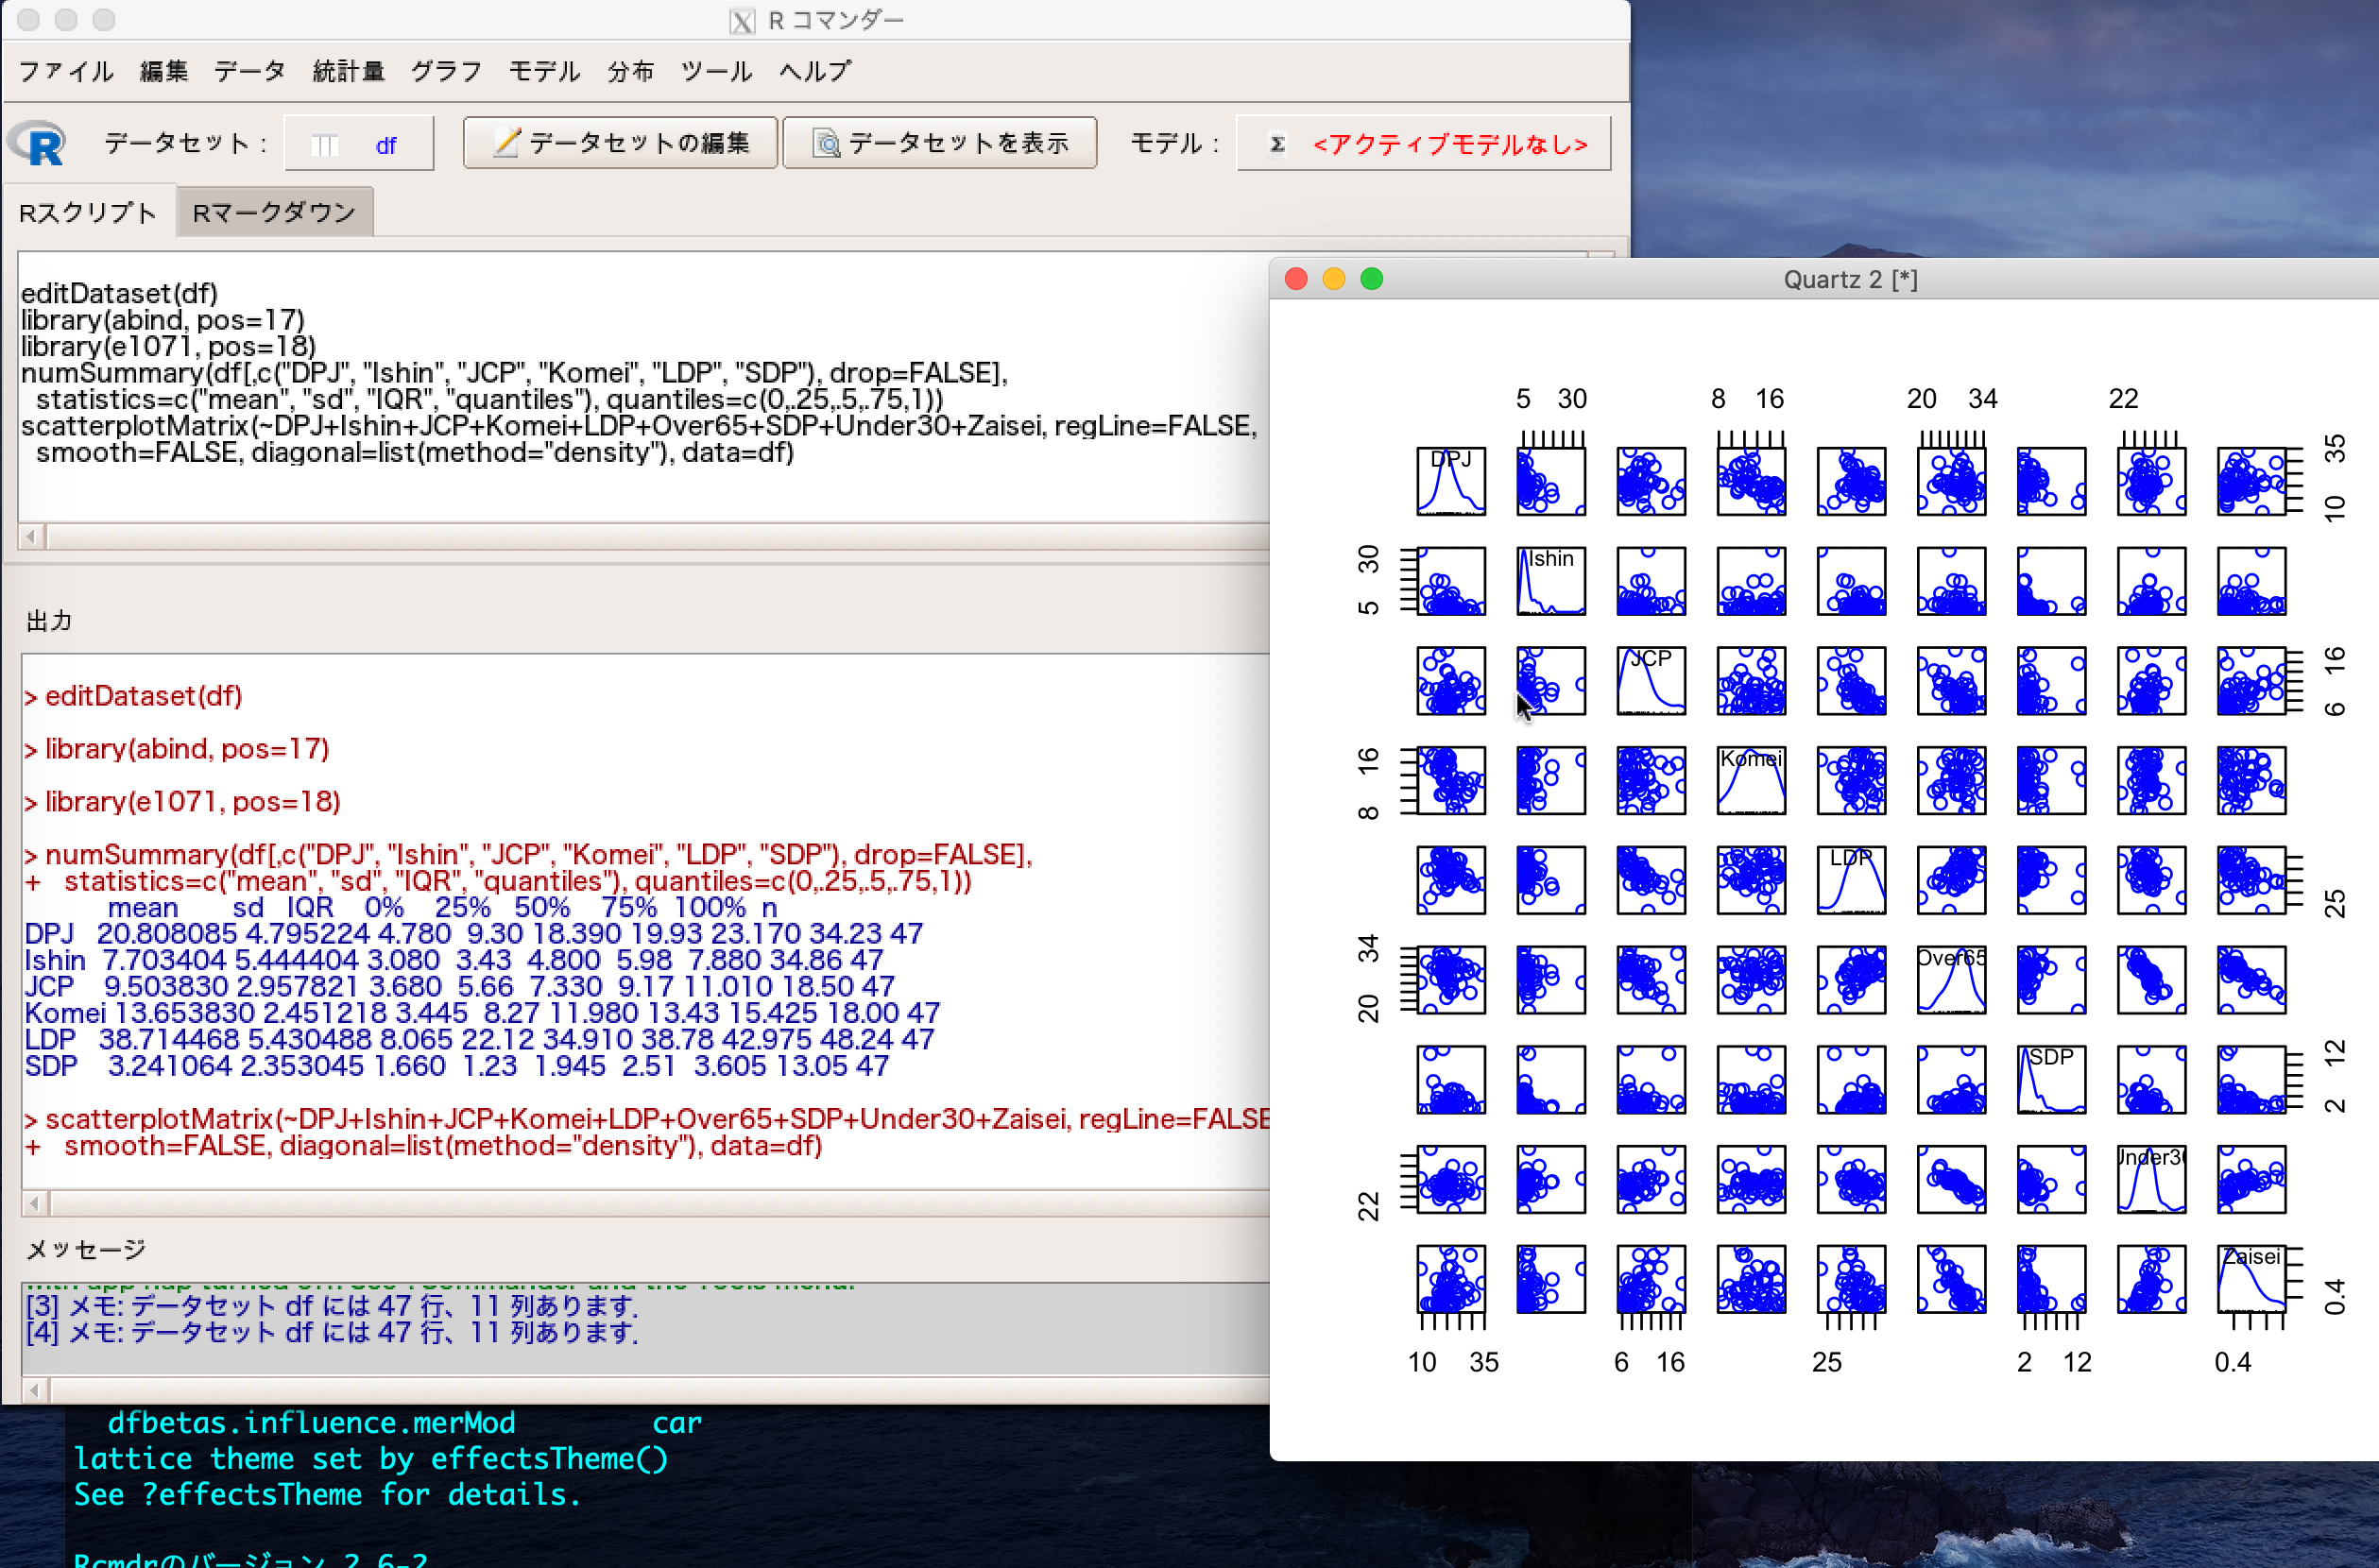
\includegraphics[width=0.75\textwidth,height=\textheight]{./Figs/AboutR/GUI_Rcmdr.png}

}

\caption{\label{fig-aboutr_rcommander}R Commander}

\end{figure}

\begin{itemize}
\tightlist
\item
  RKWard (\url{https://rkward.kde.org})
\end{itemize}

\begin{figure}

{\centering 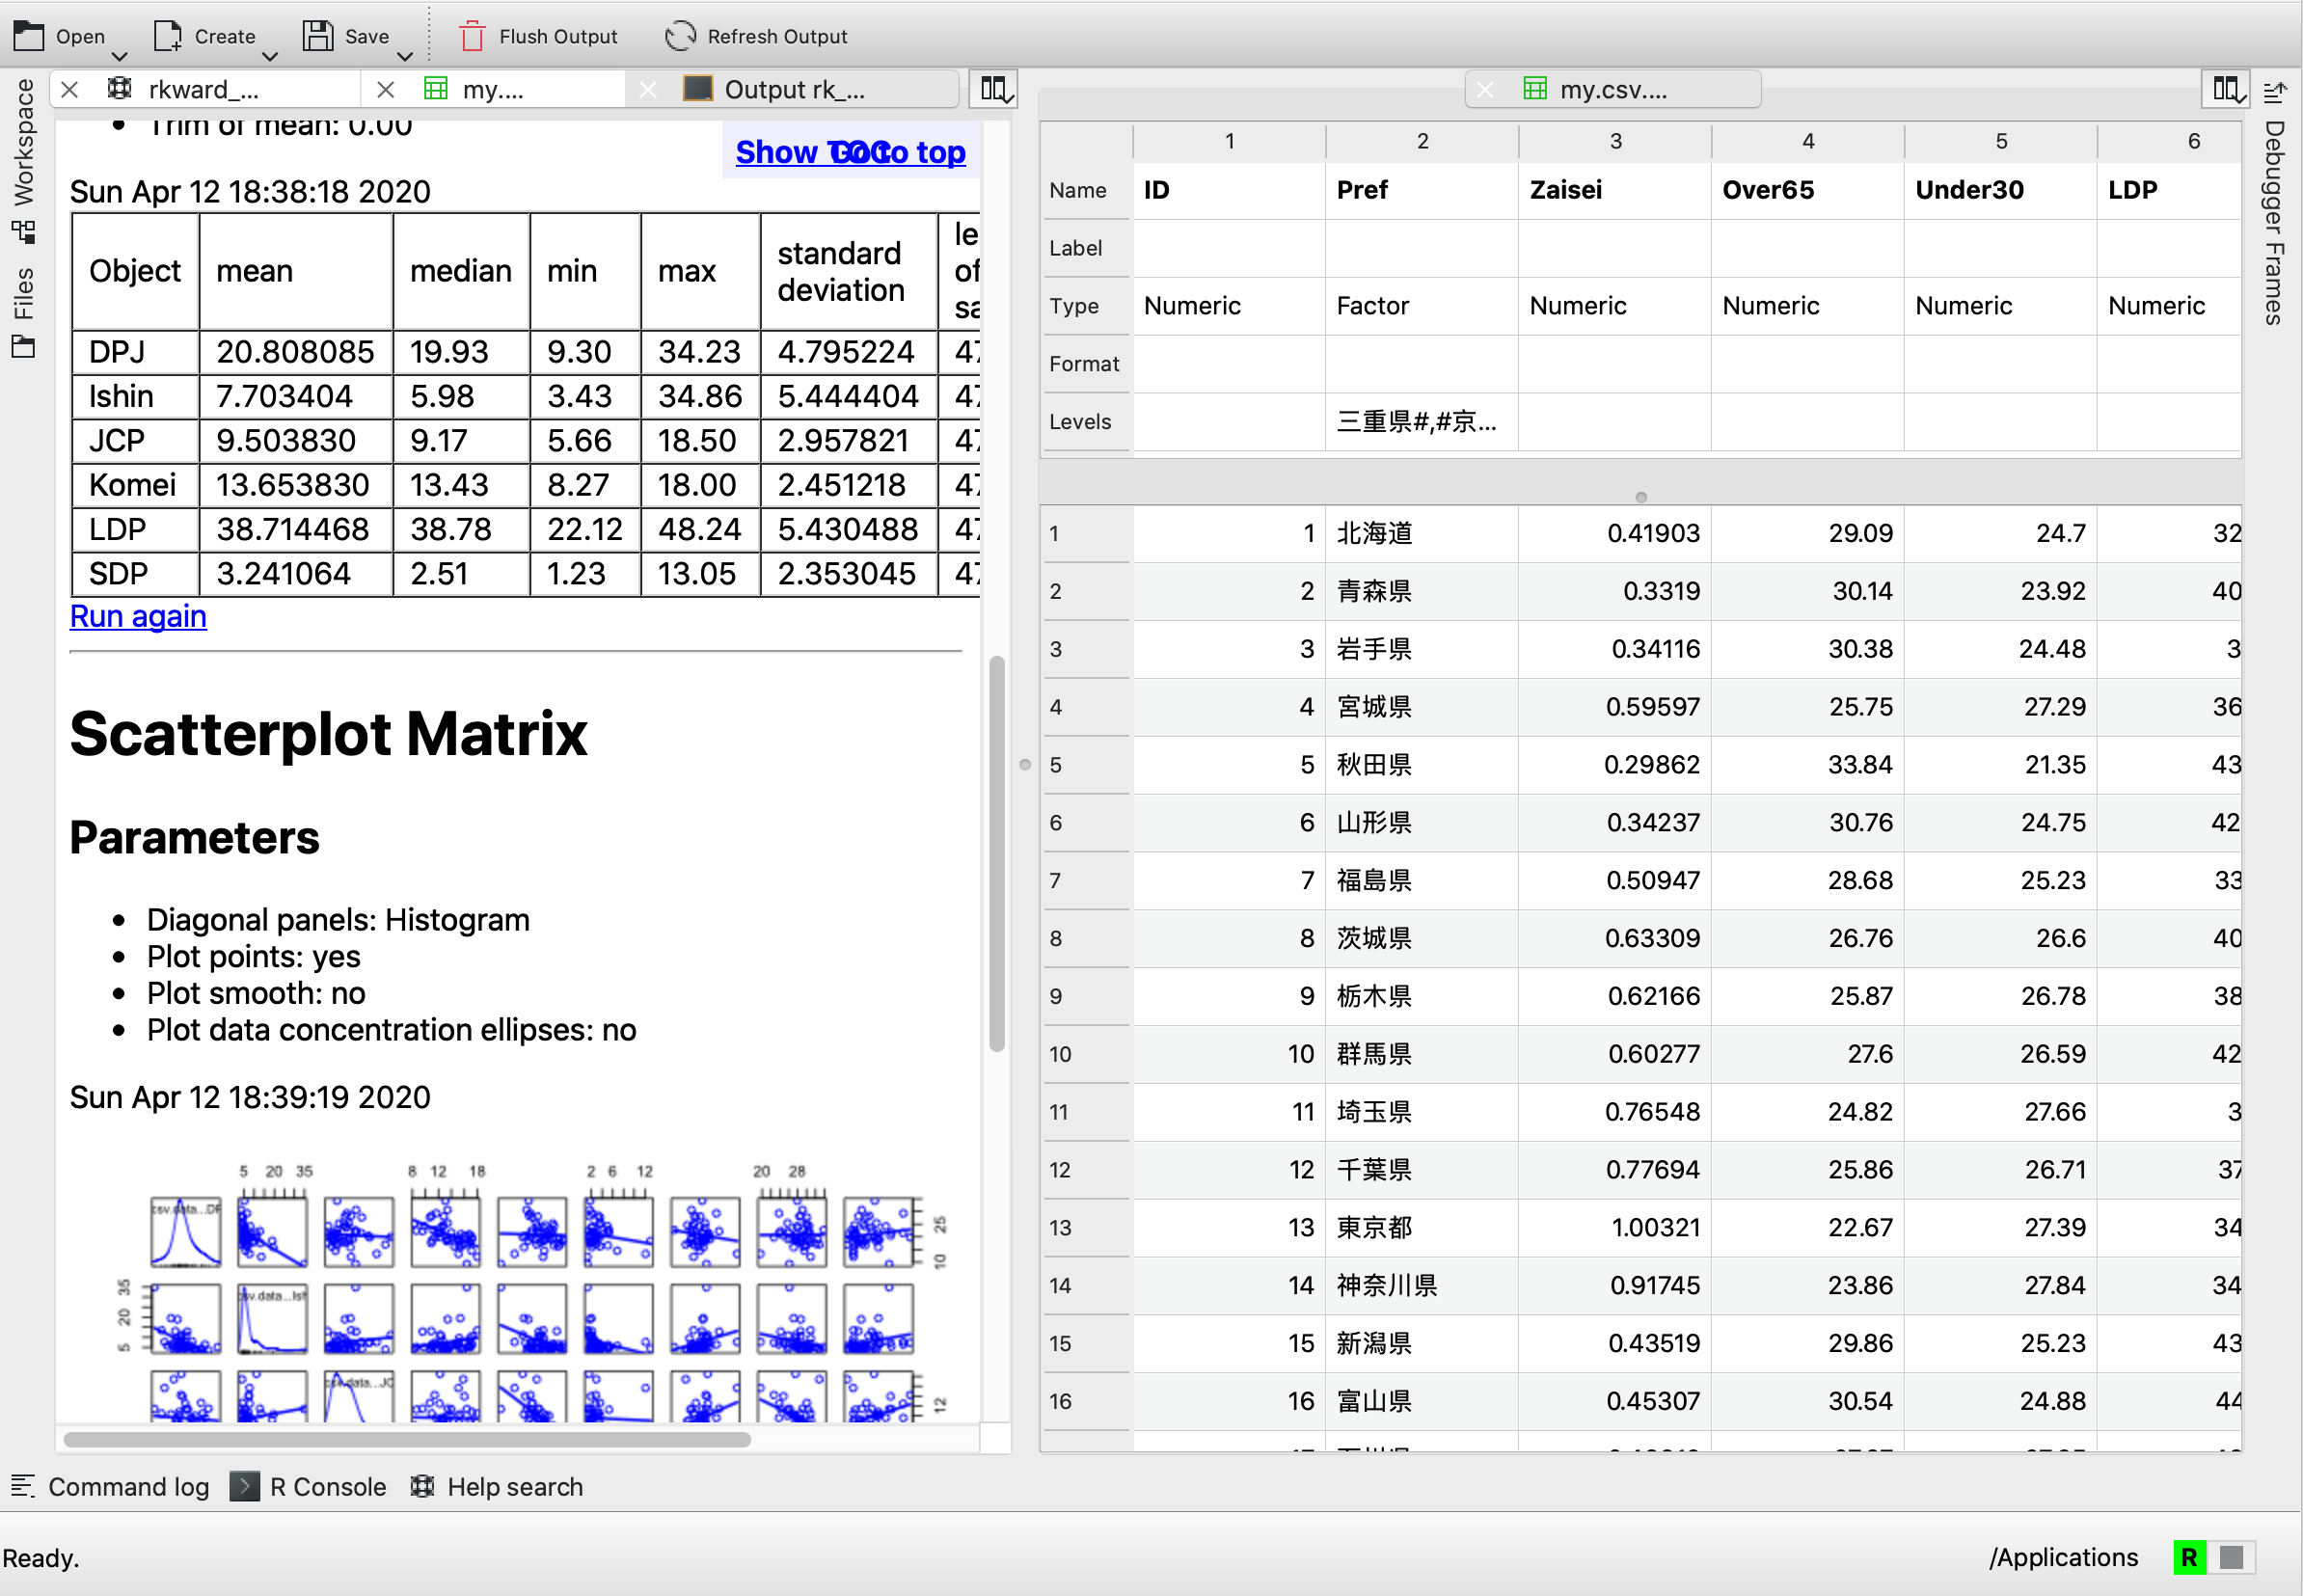
\includegraphics[width=0.75\textwidth,height=\textheight]{./Figs/AboutR/GUI_RKWard.png}

}

\caption{\label{fig-aboutr_rkward}RKWard}

\end{figure}

\begin{itemize}
\tightlist
\item
  JASP (\url{https://jasp-stats.org})
\end{itemize}

\begin{figure}

{\centering 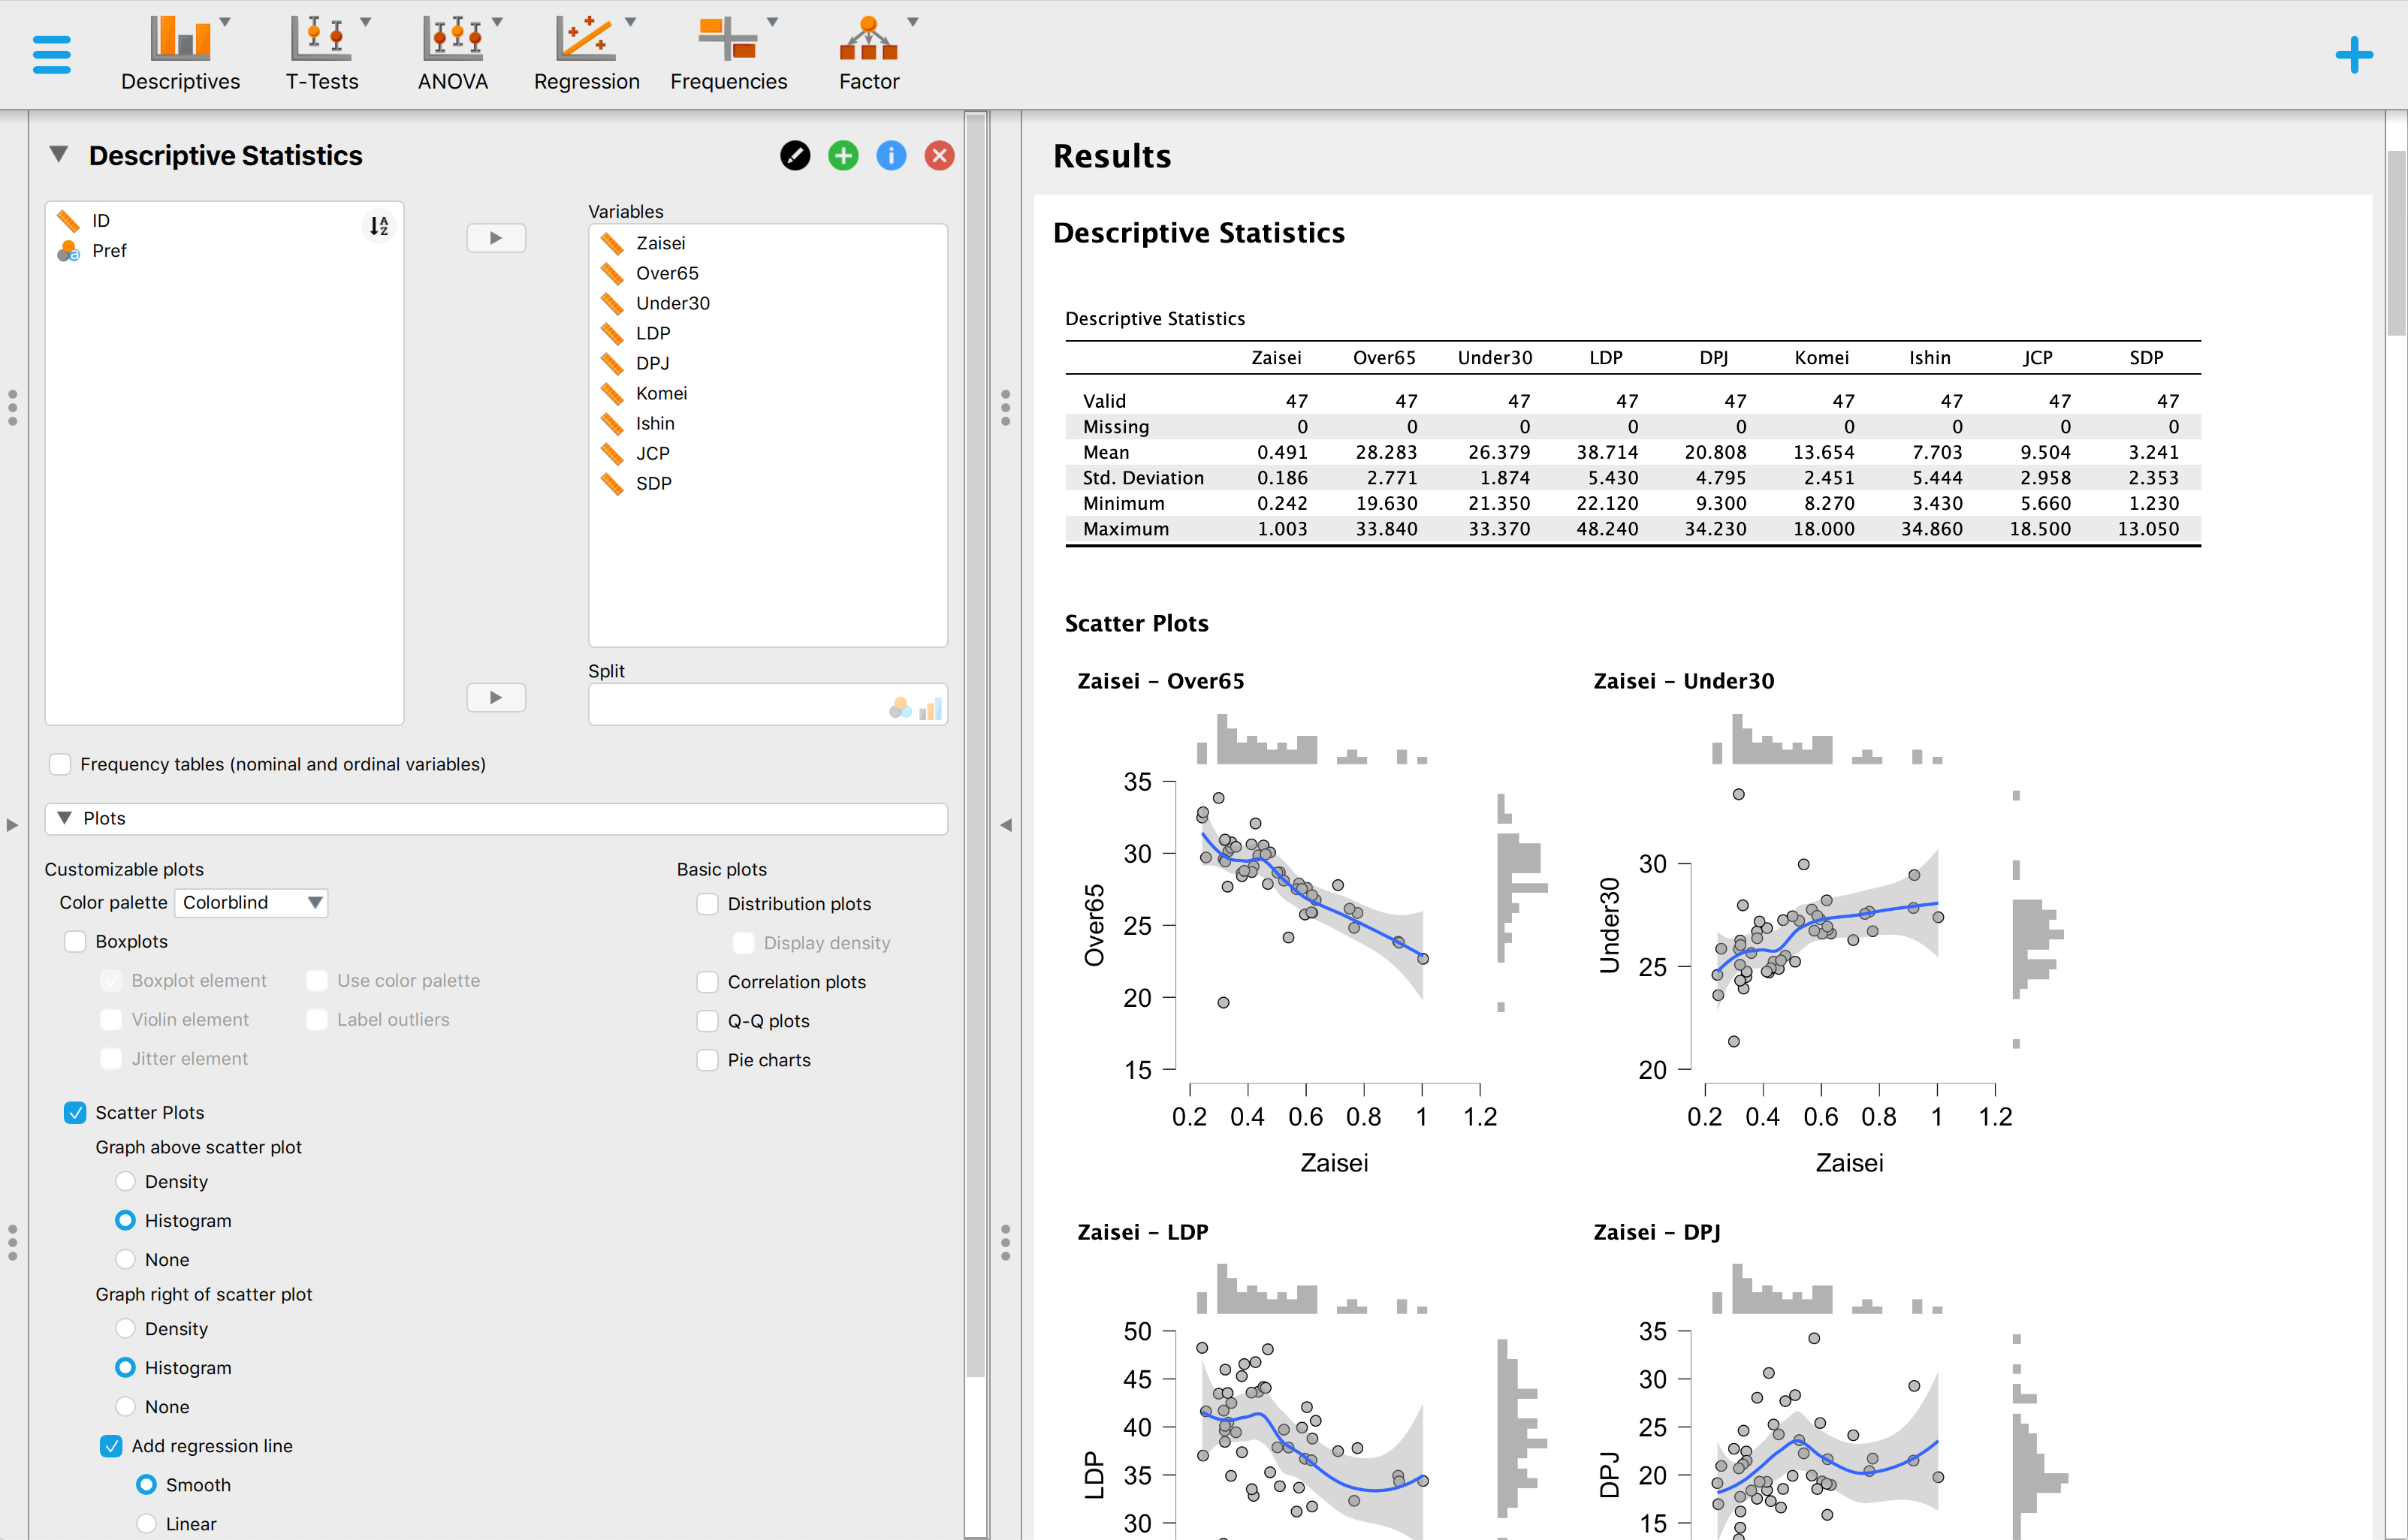
\includegraphics[width=0.75\textwidth,height=\textheight]{./Figs/AboutR/GUI_JASP.png}

}

\caption{\label{fig-aboutr_jasp}JASP}

\end{figure}

\begin{itemize}
\tightlist
\item
  jamovi (\url{https://www.jamovi.org})
\end{itemize}

\begin{figure}

{\centering 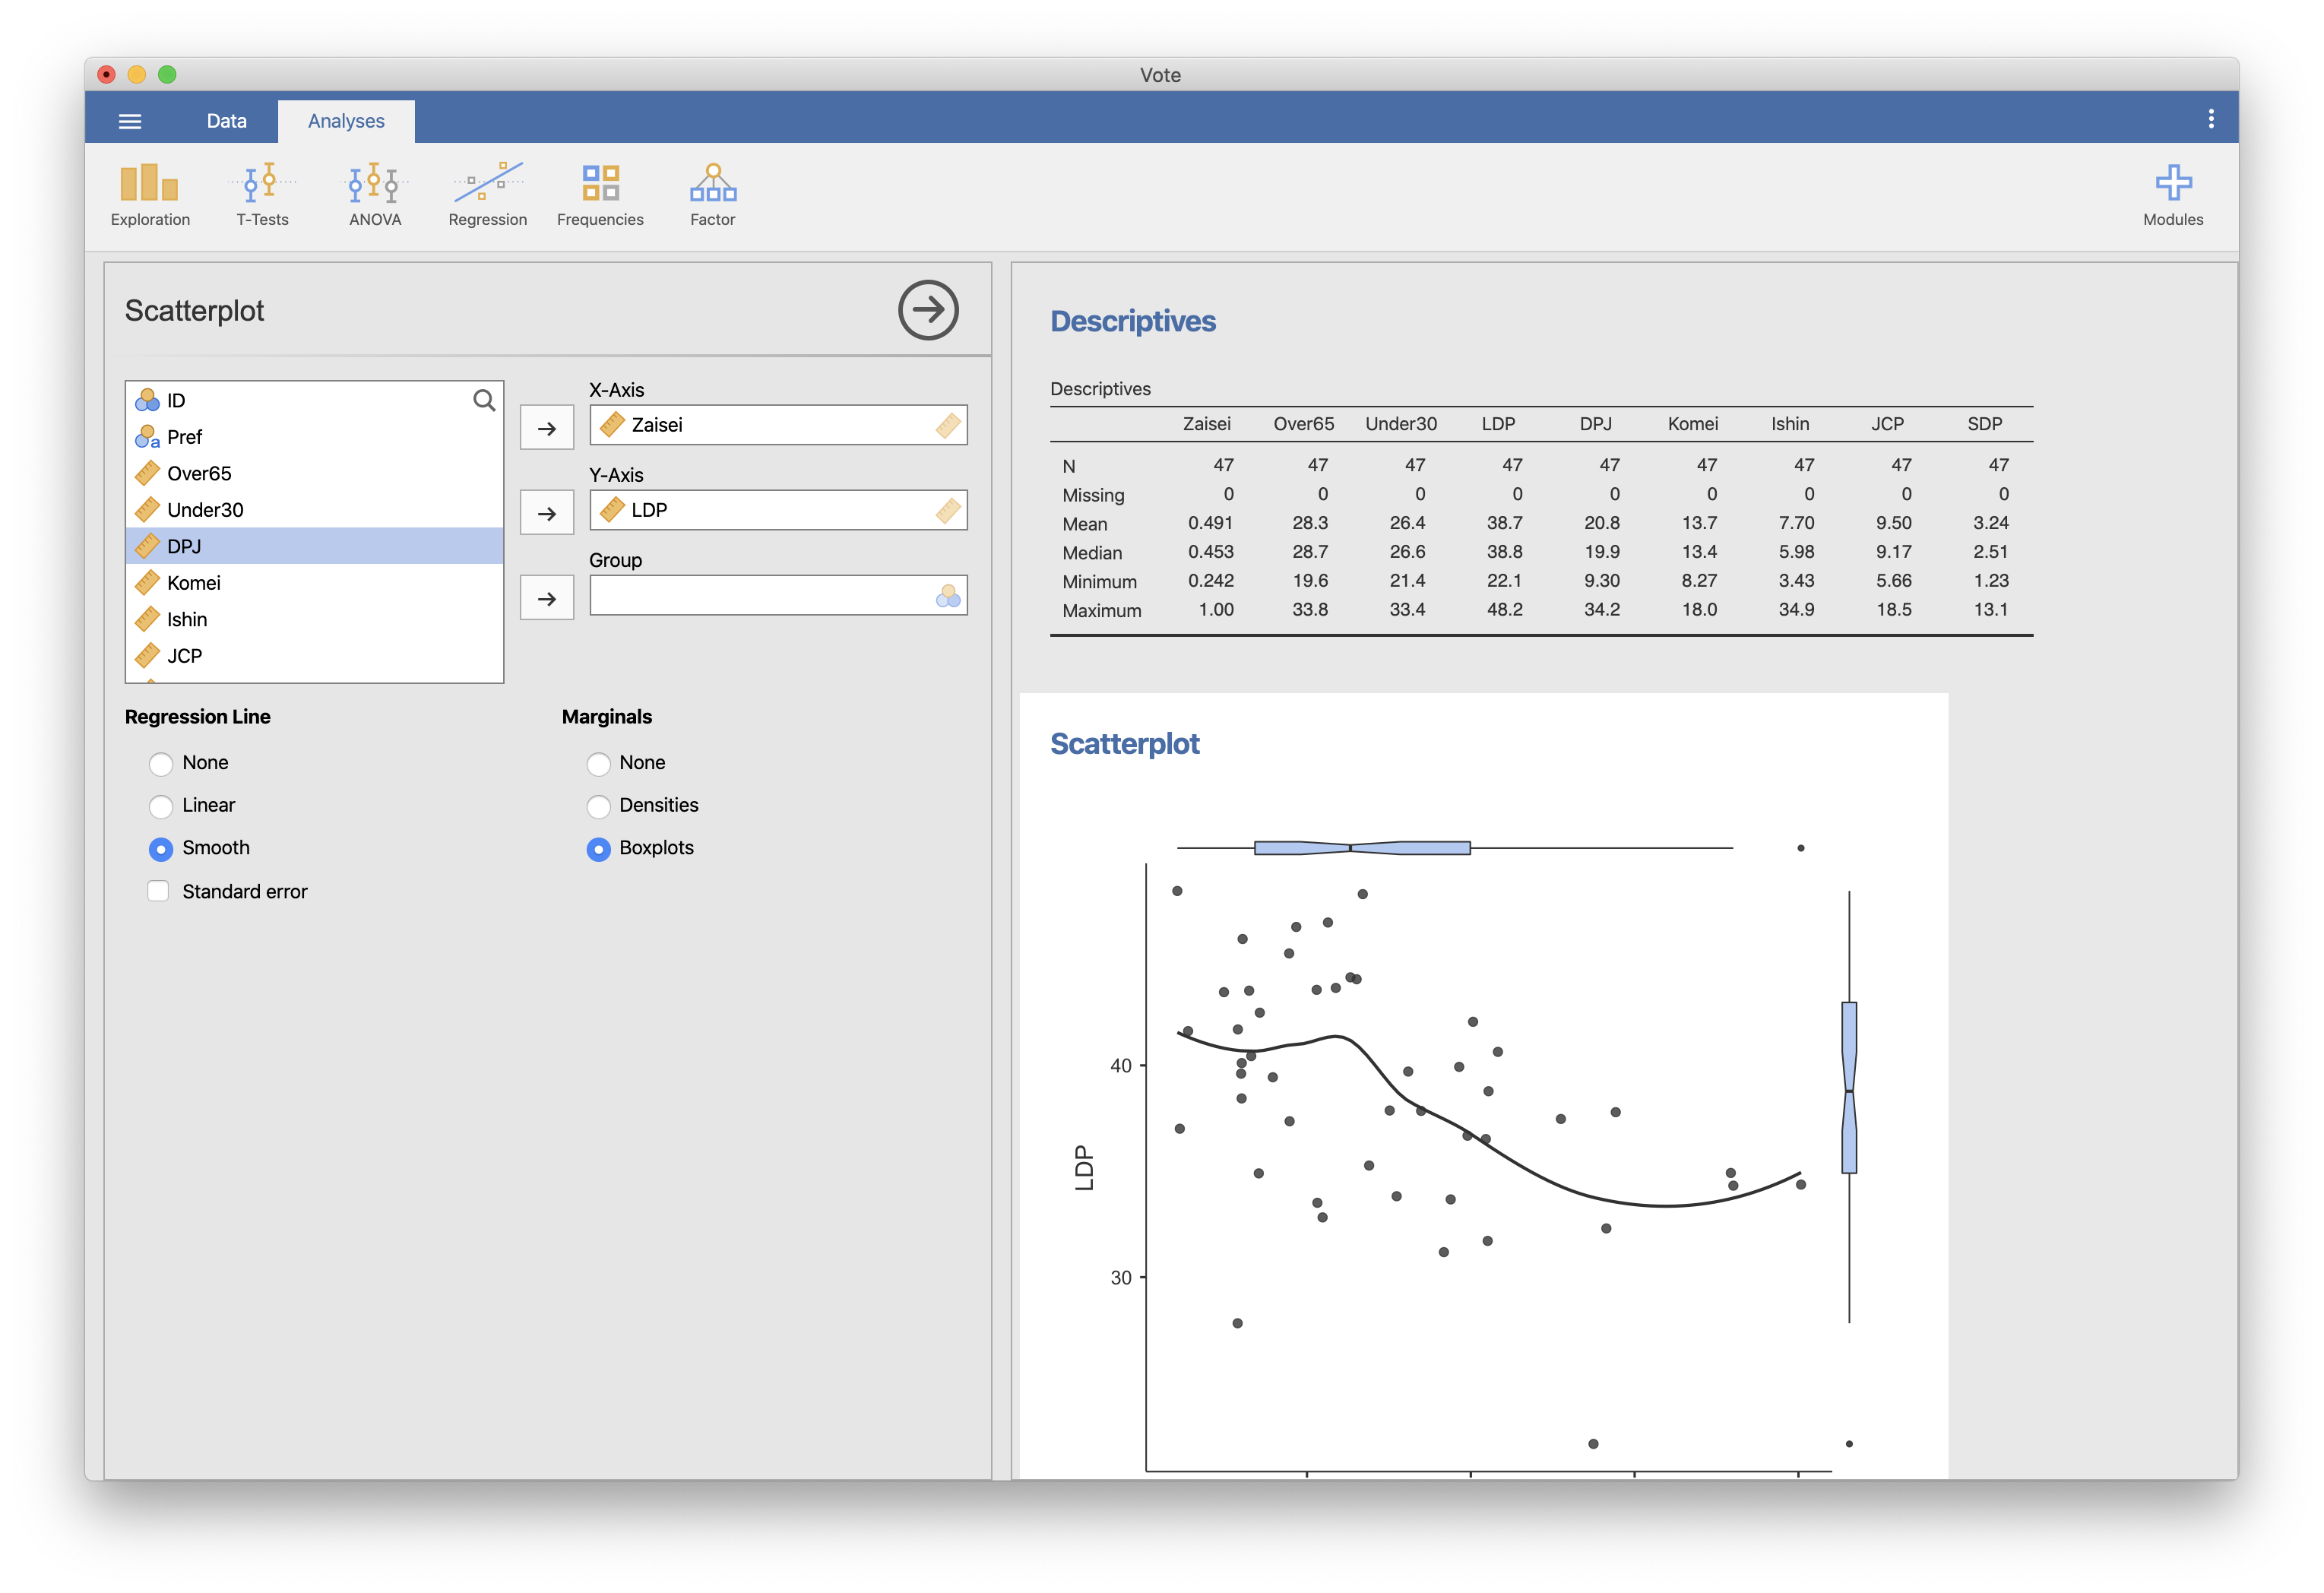
\includegraphics[width=0.75\textwidth,height=\textheight]{./Figs/AboutR/GUI_jamovi.png}

}

\caption{\label{fig-aboutr_jamovi}jamovi}

\end{figure}

\begin{itemize}
\tightlist
\item
  R AnalyticFlow (\url{https://r.analyticflow.com})
\end{itemize}

\begin{figure}

{\centering 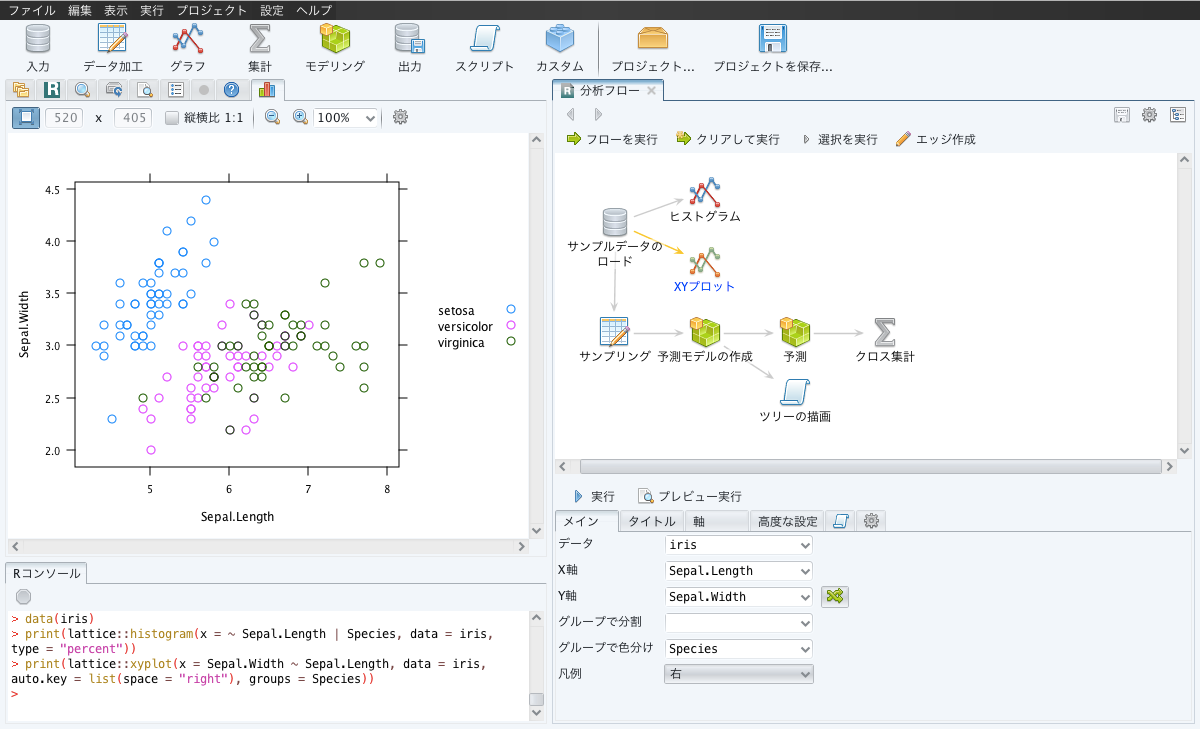
\includegraphics[width=0.75\textwidth,height=\textheight]{./Figs/AboutR/GUI_RAnalyticFlow.png}

}

\caption{\label{fig-aboutr_ranalyticflow}RAnalyticFlow}

\end{figure}

\hypertarget{aboutR-IDE}{%
\subsection{IDE}\label{aboutR-IDE}}

 プログラミングは基本的にコードを書く作業の連続だが、コードを書く他にも様々な作業を行うことになる。たとえば、自分が書いたコードの結果が正しく動作するかの確認作業や、なにか問題がある場合の対処(デバッグ)などがある。また、コードを書く際、誤字やミスなどがないかも確認する必要がある。他にもプログラムで使用されるファイルを管理しなければならない。これらの仕事を手助けしてくれるのが統合開発環境
(integrated development environment; IDE) と呼ばれるものである。

 プログラマにとって優れたIDEを使うということは、優れた秘書を雇用するようなものだ。ファイルの管理、うろ覚えのコマンドの補完入力、コードの色分けなどを自動的に行ってくれる。さらに、コードの実行結果の画面をコードと同時に表示してくれたり、これまでの作業を記録してくれるなど、多くの作業を手助けしてくれる。Rにはいくつかの優れたIDEが用意されている。本書では代表的なIDEである
\href{https://rstudio.com}{RStudio}
を使うことにする。ただし、プログラミングにIDEは必須ではない。IDEをインストールしなくても、本書を読む上で特に問題はない(RStudioに関する説明の部分を除く)が、Rの実行環境に特にこだわりがないなら
RStudioの導入を強く推奨する。

\begin{figure}

{\centering 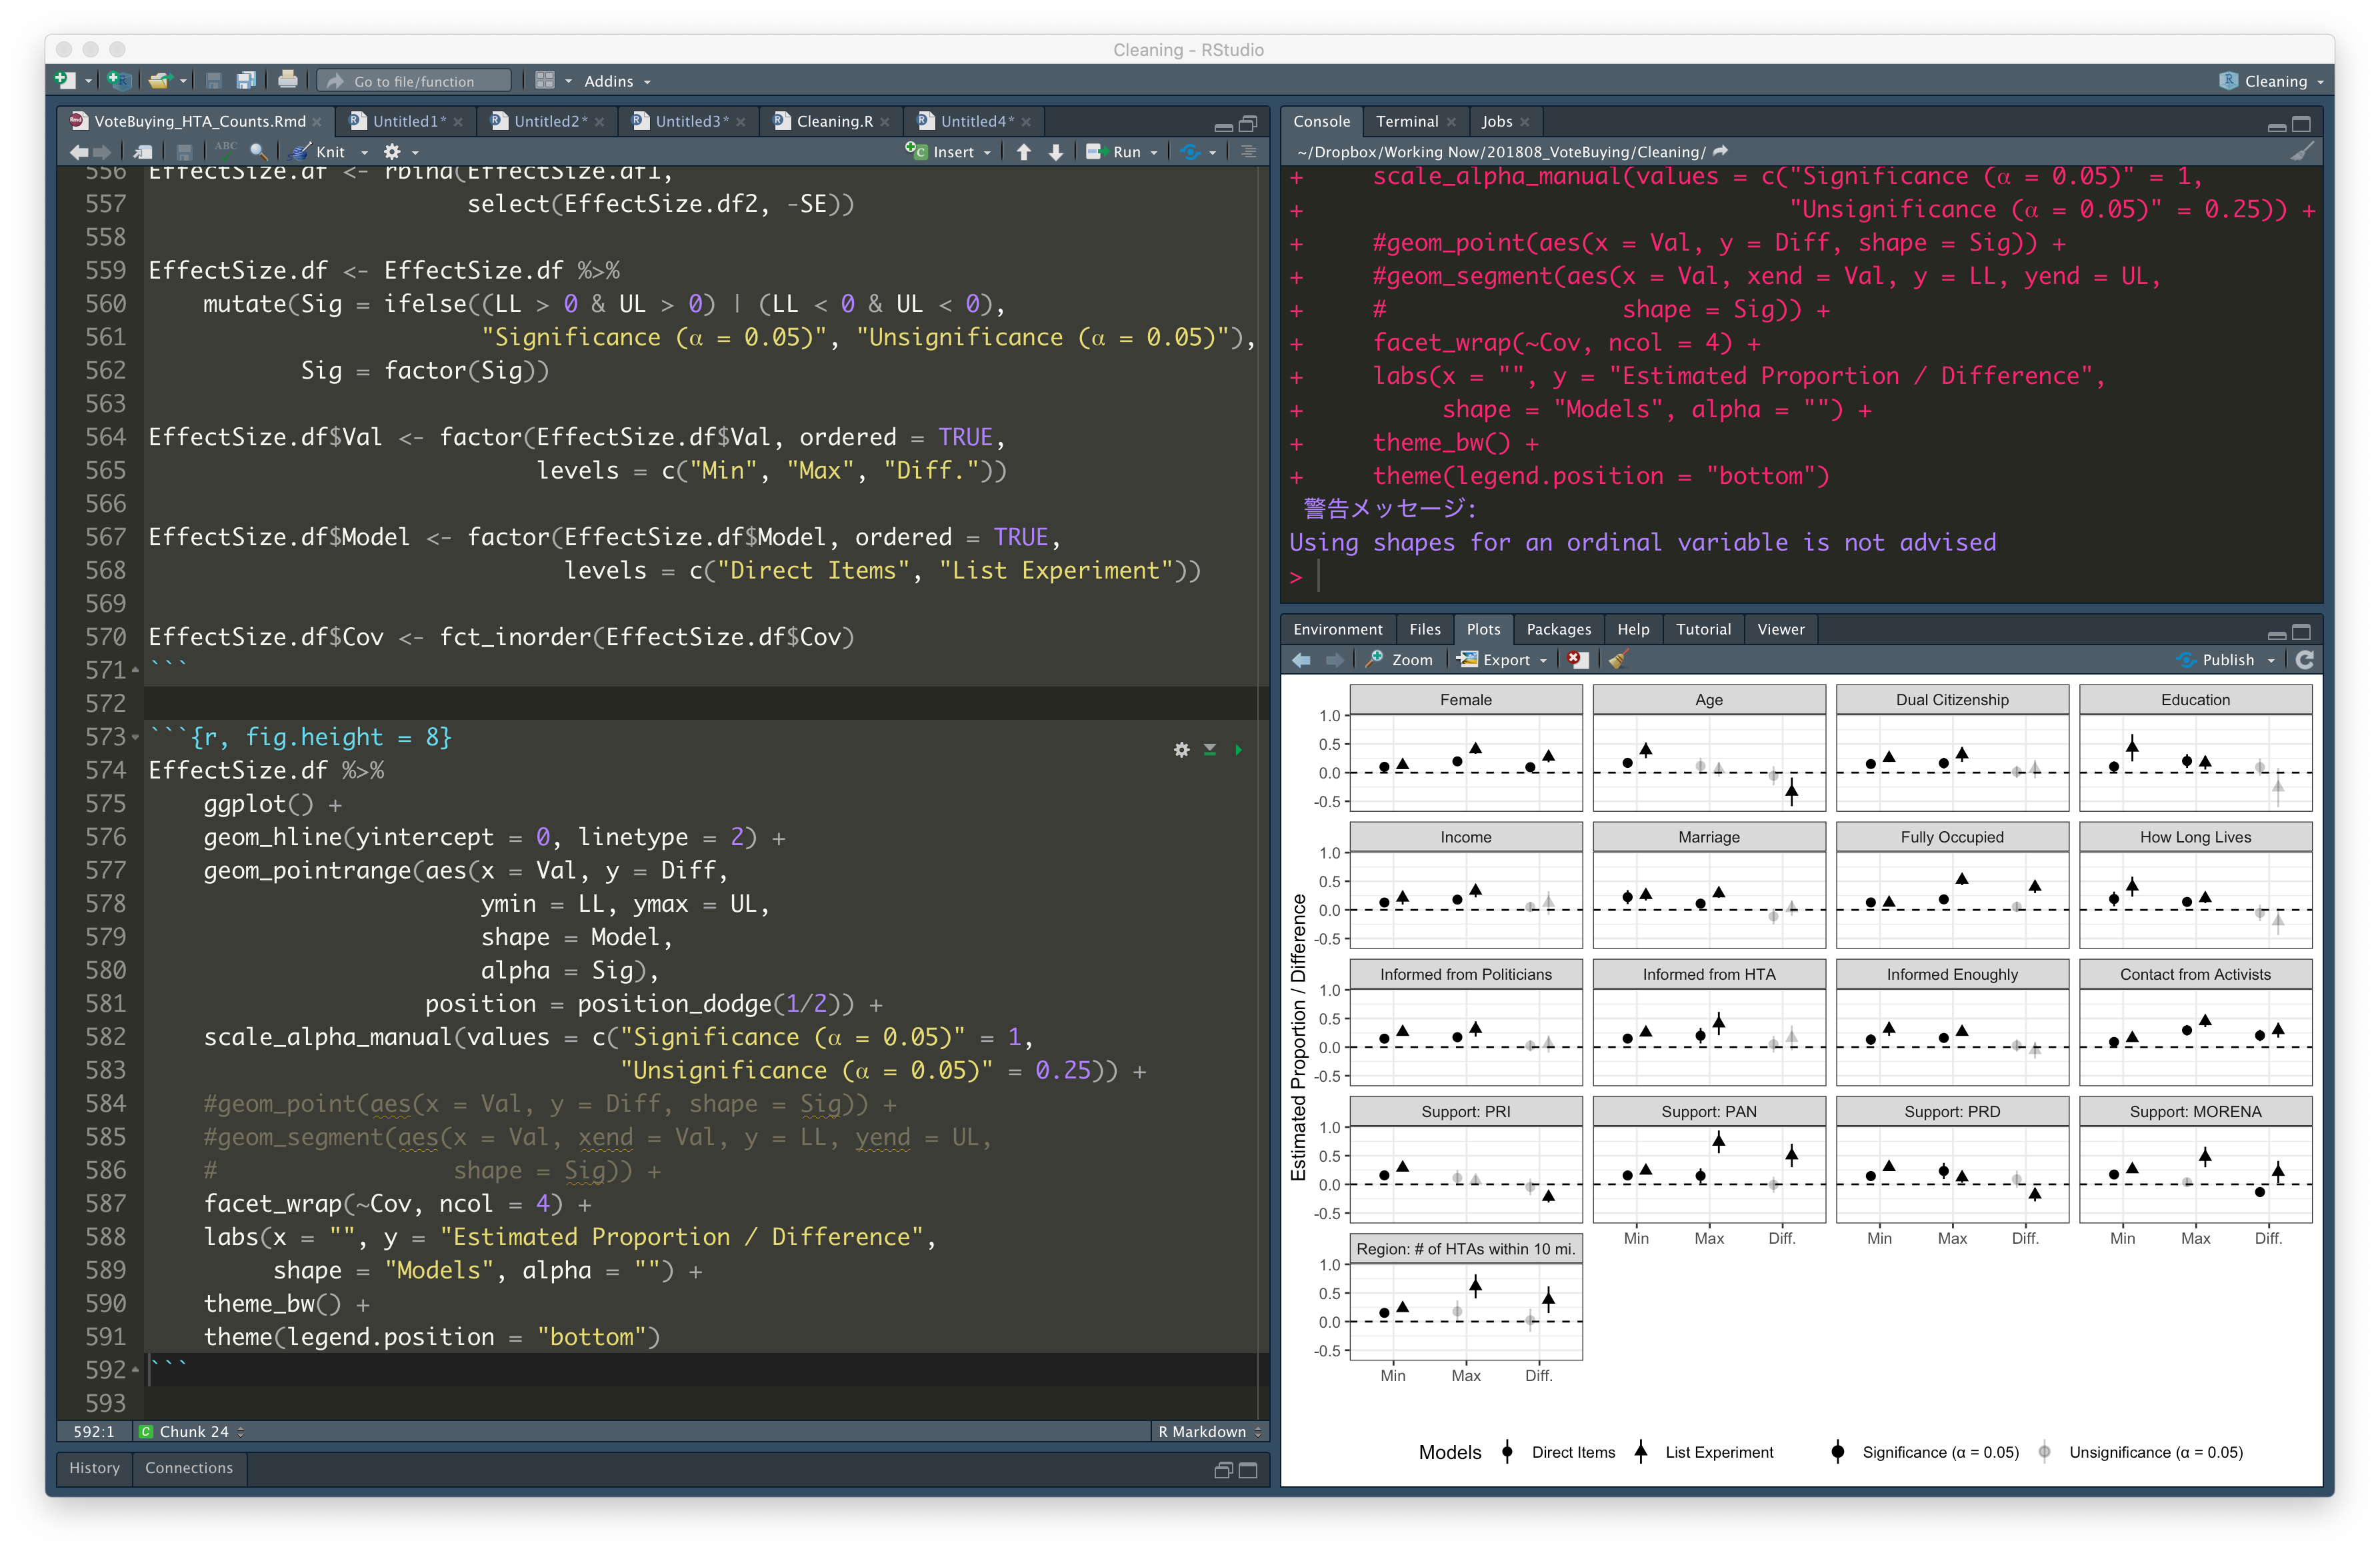
\includegraphics[width=0.75\textwidth,height=\textheight]{./Figs/AboutR/IDE_RStudio.png}

}

\caption{\label{fig-aboutr_rstudio}RStudio}

\end{figure}

 RStudio以外にもRのIDEはある。魔界において圧倒的なシェアを誇ると噂されるWindowsという名のOSを使用しているなら、\href{https://docs.microsoft.com/ja-jp/visualstudio/rtvs/installer?view=vs-2017}{R
Tools for Visual Studio} がRStudioの代替候補として有力だ。

\begin{figure}

{\centering 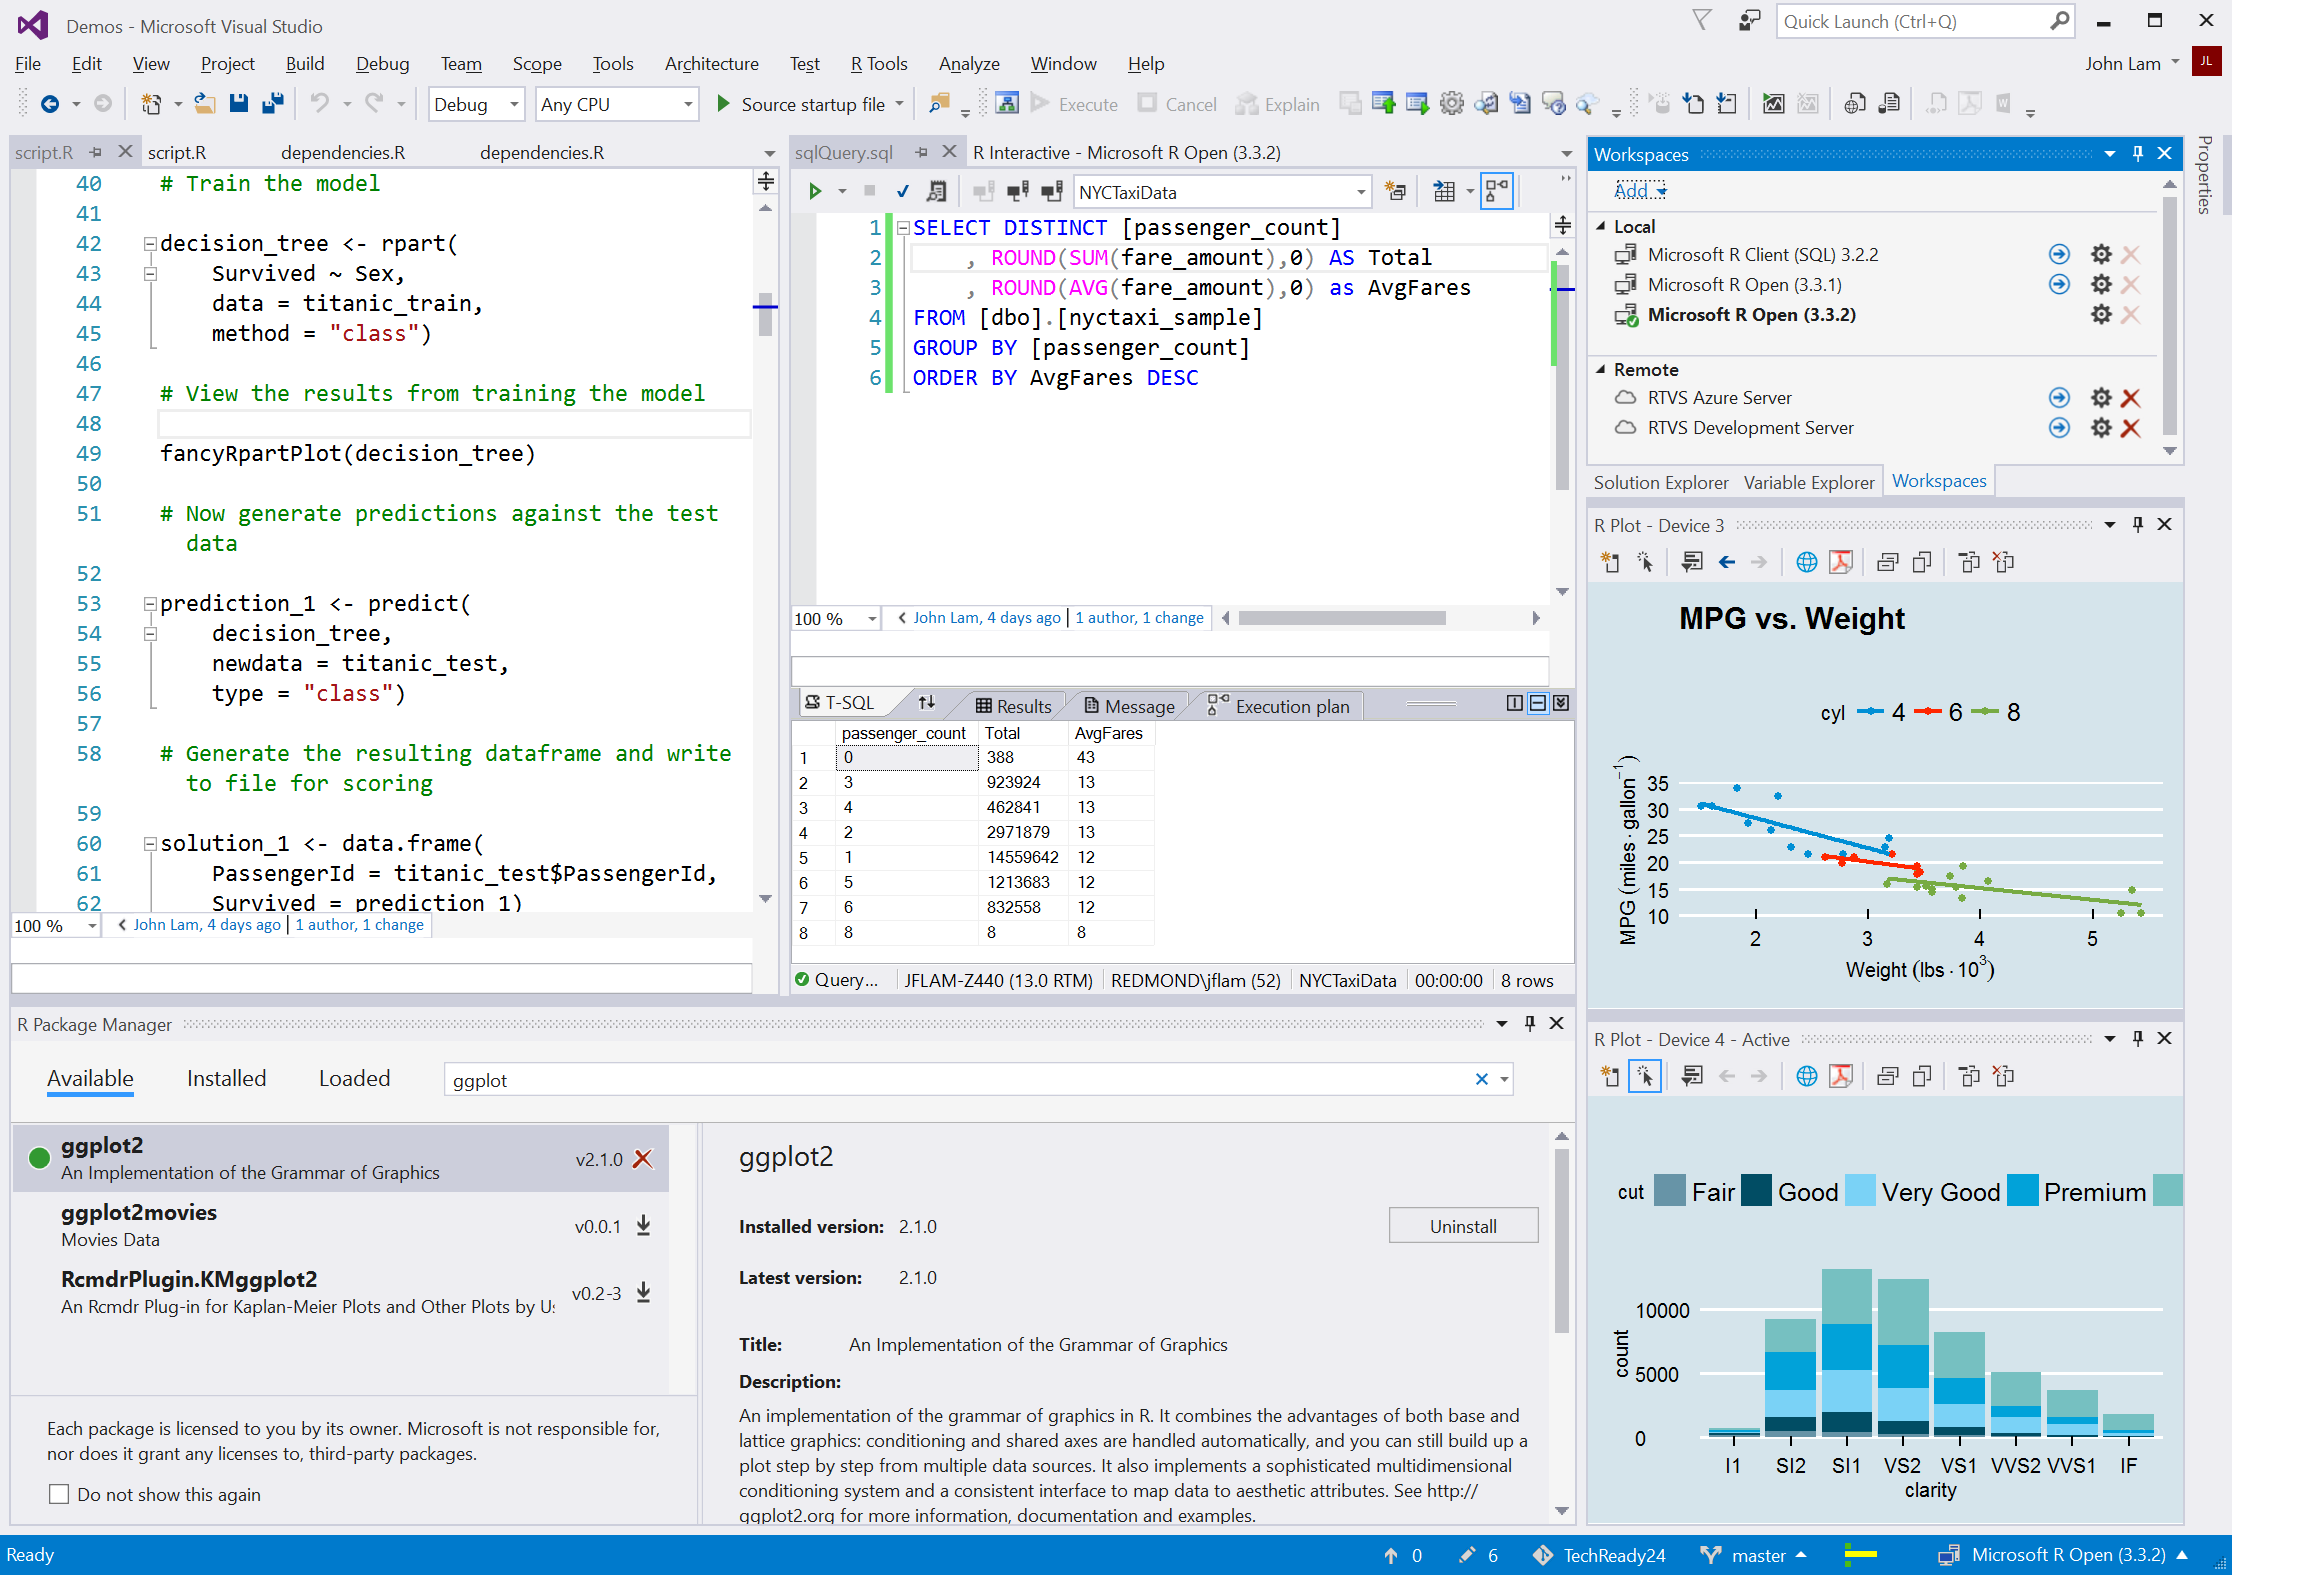
\includegraphics[width=0.75\textwidth,height=\textheight]{./Figs/AboutR/IDE_RTVS.png}

}

\caption{\label{fig-aboutr_rtvs}R Tools for Visual Studio}

\end{figure}

 自分が使い慣れたテキストエディタをIDEとして使うことも可能である。\href{https://www.sublimetext.com}{Sublime
Text} や \href{https://atom.io}{Atom} はむろん、伝統のある
\href{https://www.gnu.org/software/emacs/}{Emacs} や
\href{https://www.vim.org}{Vim} を使うこともできる。

\hypertarget{sec-installation}{%
\chapter{Rのインストール}\label{sec-installation}}

本章の内容は今後、以下の資料に基づき、再作成する予定である。

\begin{itemize}
\tightlist
\item
  矢内による資料
  (\href{https://yukiyanai.github.io/jp/resources/docs/install-R_macOS.pdf}{macOS編}、\href{https://yukiyanai.github.io/jp/resources/docs/install-R_ubuntu.pdf}{Linux
  (Ubuntu)編}、\href{https://yukiyanai.github.io/jp/resources/docs/install-R_windows.pdf}{Windows編})
\end{itemize}

\hypertarget{sec-ide}{%
\chapter{IDEの導入}\label{sec-ide}}

本章の内容は今後、以下の資料に基づき、再作成する予定である。

\begin{itemize}
\tightlist
\item
  矢内による資料
  (\href{https://yukiyanai.github.io/jp/resources/docs/install-R_macOS.pdf}{macOS編}、\href{https://yukiyanai.github.io/jp/resources/docs/install-R_ubuntu.pdf}{Linux
  (Ubuntu)編}、\href{https://yukiyanai.github.io/jp/resources/docs/install-R_windows.pdf}{Windows編})
\end{itemize}

\hypertarget{sec-customize}{%
\chapter{分析環境のカスタマイズ}\label{sec-customize}}

\hypertarget{Customize-rprofile}{%
\section{.Rprofileの設定}\label{Customize-rprofile}}

\hypertarget{Customize-rstudio}{%
\section{RStudioのカスタマイズ}\label{Customize-rstudio}}

\hypertarget{sec-packages}{%
\chapter{Rパッケージ}\label{sec-packages}}

\hypertarget{sec-packages_intro}{%
\section{パッケージとは}\label{sec-packages_intro}}

 Rには様々な関数 (functions)
が提供されている。平均値を求める\texttt{mean()}、合計を求める\texttt{sum()}、線形回帰分析を行う\texttt{lm()}、平均値の検定を行う\texttt{t.test()}などがあり、全てを列挙することはできない。しかし、データ分析の技術は日々発展し、Rがデフォルトで提供する関数では不可能ではないが、かなり長いコードが必要な分析を使わざる得ないケースもあろう。Rは開発元だけでなく、誰でも関数を作ることができる。通常なら数百行のコードが必要な分析を一行のコードで実行可能とする関数を多くのRユーザーが作ってきた。これらの関数を集めたのがパッケージである。Rにはグラフ作成に特化したパッケージ、機械学習に特化したパッケージ、テキスト分析に特化したパッケージなど、数千のパッケージが開発されている。このパッケージの豊富さがRの最大のメリットでもある。誰かが新しい分析手法を提案したら、数日内、あるいはその手法が論文として出版される前からRパッケージとして公開されるケースが多い。

 本章ではパッケージをインストールし、読み込む方法について説明する。また、パッケージの管理をアシストするパッケージ、\{pacman\}の使い方についても紹介する。

\begin{center}\rule{0.5\linewidth}{0.5pt}\end{center}

\hypertarget{sec-packages_install}{%
\section{パッケージのインストール}\label{sec-packages_install}}

 Rの環境は何かを作るための作業台に似ている。作業台にはモノを作るために材料だけでなく、工具・道具セットなども置いたりもする。この作業台がRにおける「環境
(environment)
」であり、材料がベクトルや行列、データフレームなどのデータ、工具セットがパッケージになる。データについては後で説明するとし、ここではパッケージについて考えたい。

 モノを作るためには素材・材料だけでは不十分だろう。多くの場合、なんらかの道具セットが必要となる。Rには既にいくつかの必須道具セットを用意されているが、他にも様々な道具セットがある。そして、これら道具セットには、一般的に複数の道具が含まれている。一つ一つの道具のことを、ここでは「関数
(function)
」と呼ぶ。これらの道具セットを購入し、作業台の収納に入れておくことがパッケージをインストールすることである。

\begin{Shaded}
\begin{Highlighting}[numbers=left,,]
\FunctionTok{install.packages}\NormalTok{(}\StringTok{"パッケージ名"}\NormalTok{)}
\end{Highlighting}
\end{Shaded}

 これらのパッケージは基本的に\href{https://cran.r-project.org}{CRAN}というRの公式道具屋からダウンロード・インストールされる。もう一つの大きな道具屋としては\href{https://github.com}{GitHub}がある\footnote{他にも\href{https://about.gitlab.com}{GitLab}、\href{https://bitbucket.org/product/}{Bitbucket}などがある。}。\href{https://github.com}{GitHub}は個人経営の道具屋が集まっているモールのようなものである。\href{https://github.com}{GitHub}道具屋を使用するためには、予め\href{https://cran.r-project.org}{CRAN}から\{devtools\}、または\{remotes\}というパッケージをインストールしておく必要がある。

 ここでは\{devtools\}というパッケージをインストールしてみよう。\{devtools\}はCRANに登録されているため、\texttt{install.pcakges()}関数でインストールできる。パッケージ名を\texttt{"}で囲むことを忘れないこと。

\begin{Shaded}
\begin{Highlighting}[numbers=left,,]
\FunctionTok{install.packages}\NormalTok{(}\StringTok{"devtools"}\NormalTok{)}
\end{Highlighting}
\end{Shaded}

 もし、\href{https://cran.r-project.org}{CRAN}に登録されていないパッケージを\href{https://github.com}{GitHub}からインストールするなら、\{devtools\}パッケージ、または\{remotes\}の\texttt{install\_github()}関数を使う。

\begin{Shaded}
\begin{Highlighting}[numbers=left,,]
\CommentTok{\# あらかじめ\{devtools\}、または\{remotes\}をインストールしておく}
\CommentTok{\# \{remotes\}をインストールした場合は、remotes::install\_github()を使用する}
\NormalTok{devtools}\SpecialCharTok{::}\FunctionTok{install\_github}\NormalTok{(}\StringTok{"作成者のGitHubのID/パッケージ名"}\NormalTok{)}
\end{Highlighting}
\end{Shaded}

 たとえば、筆者 (Song)
が作成しました\{\href{https://github.com/JaehyunSong/BalanceR}{BalanceR}\}パッケージがインストールしたいなら、以下のように打つ。

\begin{Shaded}
\begin{Highlighting}[numbers=left,,]
\CommentTok{\# \{remotes\}をインストールした場合は、}
\CommentTok{\# remotes::install\_github("JaehyunSong/BalanceR")}
\NormalTok{devtools}\SpecialCharTok{::}\FunctionTok{install\_github}\NormalTok{(}\StringTok{"JaehyunSong/BalanceR"}\NormalTok{)}
\end{Highlighting}
\end{Shaded}

 ここで\texttt{JaehyunSong}はSongのGitHub
IDであり、\texttt{BalanceR}はパッケージ名である。

\begin{center}\rule{0.5\linewidth}{0.5pt}\end{center}

\hypertarget{sec-packages_library}{%
\section{パッケージの読み込み}\label{sec-packages_library}}

 先ほど述べたように、パッケージのインストールは道具セットの購入と収納に似ている。ただし、実際に道具セットを使うためには、それを自分の作業台上に載せた方が効率がいいだろう\footnote{\texttt{mean()}や\texttt{sum()}、\texttt{lm()}のように、よく使われる関数
  (=工具)はR起動と同時に作業台上に載せられる。}
\footnote{作業台上に載せずに、収納から必要な時だけ道具を取り出して使うことも可能である。この場合、\texttt{パッケージ名::関数名()}のように関数を使う。よく使うパッケージなら読み込んだ方が効率的だが、1、2回くらいしか使わないパッケージなら、このような使い方も良いだろう。}。この作業がパッケージの読み込み
(load)
である。インストールしたパッケージを読み込むには\texttt{library()}または\texttt{require()}関数を使う。\texttt{require()}は関数内に使う目的で設計された関数だが、パッケージを読み込むという点では全く同じである。

\begin{figure}

{\centering 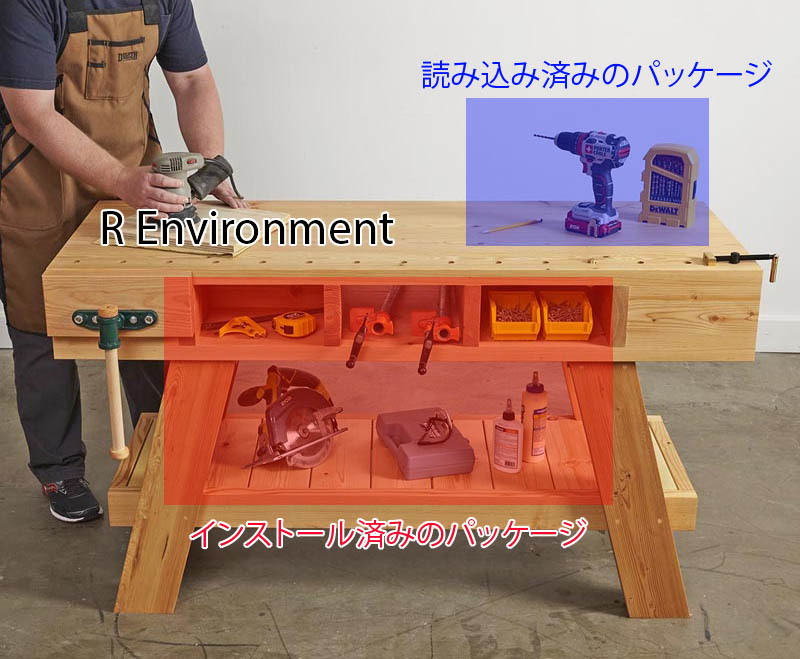
\includegraphics[width=0.75\textwidth,height=\textheight]{./Figs/Installation/Package_Workbench.jpg}

}

\caption{\label{fig-installation_package}パッケージのイメージ}

\end{figure}

\begin{Shaded}
\begin{Highlighting}[numbers=left,,]
\FunctionTok{library}\NormalTok{(}\StringTok{"パッケージ名"}\NormalTok{)}
\CommentTok{\#または}
\FunctionTok{require}\NormalTok{(}\StringTok{"パッケージ名"}\NormalTok{)}
\end{Highlighting}
\end{Shaded}

 読み込まれたパッケージはセッションが開かれている時のみに有効である。一通りの作業が終わり、作業部屋から退出すると、作業台上の道具セットは収納に自動的に戻される。つまり、RまたはRStudioを閉じると読み込まれたパッケージは自動的に取り外されるということである。しかし、作業の途中に読み込んだパッケージをセッションから取り外したい時があるかも知れない。この場合、\texttt{detach()}関数を使う。

\begin{Shaded}
\begin{Highlighting}[numbers=left,,]
\FunctionTok{detach}\NormalTok{(}\StringTok{"パッケージ名"}\NormalTok{)}
\end{Highlighting}
\end{Shaded}

\begin{center}\rule{0.5\linewidth}{0.5pt}\end{center}

\hypertarget{sec-packages_update}{%
\section{パッケージのアップデート}\label{sec-packages_update}}

 Rパッケージはバグが修正されたり、新しい機能 (=関数)
が追加されるなど、日々更新される。できる限りパッケージは最新版に維持した方が良いだろう。パッケージのアップデートはパッケージのインストールと同じである。\{dplyr\}というパッケージを最新版にアップデートしたい場合、\texttt{install.packages("dplyr")}で十分である。

 しかし、Rを使っていくうちに数十個のパッケージをインストールしていくこととなり、一つ一つアップデートするのは面倒だろう。そもそも既に最新版が入っていて
(または開発休止/中止)、アップデートが不要なパッケージがあるかも知れない。実はRStudioを使えば、アップデートが必要なパッケージのリストが表示され、一気にアップデートすることができる。RStudioのPackagesペインにある「Update」をクリックしてみれば、アップデート可能なパッケージの一覧が表示される。ここでアップデートしたいパッケージの左にチェックをするか、下段の「Select
All」を選択して「Install
Updates」をクリックすれば、チェックされているパッケージがアップデートされる。

 ただし、場合によってはアップデート時、以下のようなメッセージがコンソールに表示されるかも知れない。

\begin{verbatim}
  There are binary versions available but the source versions
  are later:
      binary source needs_compilation
terra 1.5-17 1.5-21              TRUE
yaml   2.2.2  2.3.4              TRUE

Do you want to install from sources the packages which need compilation? (Yes/no/cancel)
\end{verbatim}

 \textbf{コンソール}にYes、no、cancelのいずれかを入力してReturnキー
(Enterキー)を押す必要がある。どうしても最新のパッケージが欲しい場合はYesを入力すれば良いが、インストールに時間がかかる場合がある。一方、noを入力した場合は、若干古いバージョンがインストールされるが、インストールに必要な時間が短いため、基本的にはnoでも問題ないだろう。cancelを入力した場合はアップデートが全てキャンセルされる。

\begin{center}\rule{0.5\linewidth}{0.5pt}\end{center}

\hypertarget{sec-packages_pacman}{%
\section{\{pacman\}によるパッケージ管理}\label{sec-packages_pacman}}

\begin{Shaded}
\begin{Highlighting}[numbers=left,,]
\FunctionTok{install.packages}\NormalTok{(}\StringTok{"pacman"}\NormalTok{)}
\end{Highlighting}
\end{Shaded}

\hypertarget{ux30a4ux30f3ux30b9ux30c8ux30fcux30eb}{%
\subsection{インストール}\label{ux30a4ux30f3ux30b9ux30c8ux30fcux30eb}}

 パッケージをCRANからインストールには\texttt{p\_install()}関数を使用する。使い方は\texttt{install.packages()}と同じであり、複数のパッケージをインストールしたい場合はパッケージ名の箇所に\texttt{c(パッケージ名1,\ パッケージ名2,\ ...)}を入れる。パッケージ名は\texttt{"}で囲んでも、囲まなくても良い。GitHubに公開されているパッケージは\texttt{p\_install\_gh()}関数を使用する。これは\{devtools\}、または\{remotes\}の\texttt{install\_github()}と同じ使い方となり、必ず\texttt{"}で囲む必要がある。

 これらの関数を使う際、わざわざ\texttt{library(pacman)}を使う必要はない。パッケージのインストールや、読み込みなどはコード内に何回も使われることがほとんどないため、\{pacman\}を読み込まず\texttt{pacman::関数名()}で当該関数を使うことができる。

\begin{Shaded}
\begin{Highlighting}[numbers=left,,]
\CommentTok{\# CRANからインストール}
\NormalTok{pacman}\SpecialCharTok{::}\FunctionTok{p\_install}\NormalTok{(パッケージ名)}
\CommentTok{\# githubからインストール}
\NormalTok{pacman}\SpecialCharTok{::}\FunctionTok{p\_install\_gh}\NormalTok{(}\StringTok{"作成者のGitHubのID/パッケージ名"}\NormalTok{) }
\end{Highlighting}
\end{Shaded}

\hypertarget{ux8aadux307fux8fbcux307f}{%
\subsection{読み込み}\label{ux8aadux307fux8fbcux307f}}

 パッケージの読み込みには\texttt{p\_load()}関数を使い、実はこの関数は\{pacman\}を使う最も大きな要素である。\texttt{p\_load()}関数の使い方は以下の通りである。

\begin{Shaded}
\begin{Highlighting}[numbers=left,,]
\NormalTok{pacman}\SpecialCharTok{::}\FunctionTok{p\_load}\NormalTok{(パッケージ名)}
\end{Highlighting}
\end{Shaded}

 \texttt{p\_load()}の便利なところは (1)
複数のパッケージが指定可能であることと、 (2)
インストールされていないパッケージはCRANから自動的にインストールして読み込んでくれる点だ。たとえば、\{tidyverse\}と\{broom\}、\{estimatr\}という3つのパッケージを読み込む場合、\texttt{library()}関数を使うと以下のようになる。

\begin{Shaded}
\begin{Highlighting}[numbers=left,,]
\CommentTok{\# library() を使う場合}
\FunctionTok{library}\NormalTok{(tidyverse)}
\FunctionTok{library}\NormalTok{(broom)}
\FunctionTok{library}\NormalTok{(estimatr)}
\end{Highlighting}
\end{Shaded}

 一方、\{pacman\}の\texttt{p\_load()}を使えば、以下のように3つのパッケージを読み込むことができる。

\begin{Shaded}
\begin{Highlighting}[numbers=left,,]
\CommentTok{\# \{pacman\}のp\_load() を使う場合}
\NormalTok{pacman}\SpecialCharTok{::}\FunctionTok{p\_load}\NormalTok{(tidyverse, broom, estimatr)}
\end{Highlighting}
\end{Shaded}

 また、\texttt{p\_load()}内のパッケージがインストールされていない場合、CRANのパッケージリストから検索し、そのパッケージをインストールしてくれる。したがって、上で紹介した\texttt{p\_install()}は実質的に使うケースはほぼない。ただし、GitHub上のパッケージは自動的にインストールしてくれない。たとえば、GitHub上のみにて公開されている\{BlanceR\}パッケージがインストールされていない場合、\texttt{p\_load(BalanceR)}を実行しても\{BalanceR\}はインストールされない\footnote{GitHubからパッケージを検索し、インストール\&読み込みをする\texttt{p\_load\_gh()}という関数もある。たとえば、\texttt{pacman::p\_load\_gh("JaehyunSong/BalanceR")}を実行した場合、\{BalanceR\}パッケージがインストールされていると読み込みのみ行い、インストールされていない場合はJaehyunSongレポジトリから\{BalanceR\}をインストールし、読み込む。コードの最上段に\texttt{p\_load()}を使うなら、\texttt{p\_load()}と\texttt{p\_load\_gh()}を分けて記述するのも良いだろう。}。あらかじめ\texttt{p\_install\_gh()}でインストールしておく必要がある。

\hypertarget{ux30a2ux30c3ux30d7ux30c7ux30fcux30c8}{%
\subsection{アップデート}\label{ux30a2ux30c3ux30d7ux30c7ux30fcux30c8}}

 \{pacman\}にはアップデートが可能なパッケージを全てアップデートしてくれる\texttt{p\_update()}という関数も用意されている。使い方は簡単で、コンソール上に\texttt{p\_update()}のみの入力すれば良い。ただし、一部のパッケージのみをアップデートしたいのであれば、RStudioが提供するアップデート機能を使った方が良いかも知れない\footnote{\texttt{p\_update(ask\ =\ TRUE)}を実行すれば個々のパッケージに対してアップデートするかどうかを決めることができるが、面倒である。}。

 また、同じ機能の関数として\texttt{p\_up()}があるが、コードの可読性のために\texttt{p\_update()}の方を推奨したい。

\begin{Shaded}
\begin{Highlighting}[numbers=left,,]
\NormalTok{pacman}\SpecialCharTok{::}\FunctionTok{p\_update}\NormalTok{()}
\end{Highlighting}
\end{Shaded}

\begin{center}\rule{0.5\linewidth}{0.5pt}\end{center}

\hypertarget{sec-packages_tidyverse}{%
\section{必須パッケージのインストール}\label{sec-packages_tidyverse}}

 ここでは現在のRにおいて必須パッケージである\{tidyverse\}をインストールする。\{tidyverse\}は\{dplyr\}、\{ggplot2\}、\{tidyr\}など、Rにおいて不可欠なパッケージを含むパッケージ\textbf{群}である。また、上で紹介した\{devtools\}も今のうちにインストールしておこう。既に導入済みの読者は走らせなくても良い。

\begin{Shaded}
\begin{Highlighting}[numbers=left,,]
\FunctionTok{install.packages}\NormalTok{(}\StringTok{"tidyverse"}\NormalTok{)}
\FunctionTok{install.packages}\NormalTok{(}\StringTok{"devtools"}\NormalTok{)}
\end{Highlighting}
\end{Shaded}

\part{Rの基礎}

\hypertarget{sec-rbasic}{%
\chapter{基本的な操作}\label{sec-rbasic}}

\hypertarget{sec-rbasic_compbasic}{%
\section{コンピュータの基礎知識}\label{sec-rbasic_compbasic}}

 Rを使い始める前に、コンピュータについて最低限知っておいてほしい基礎知識について説明する。

\hypertarget{ux30d5ux30a1ux30a4ux30ebux540d}{%
\subsection{ファイル名}\label{ux30d5ux30a1ux30a4ux30ebux540d}}

 まず、コンピュータ上のファイル名について説明する。

\hypertarget{ux30d5ux30a1ux30a4ux30ebux540dux62e1ux5f35ux5b50}{%
\subsubsection{ファイル名拡張子}\label{ux30d5ux30a1ux30a4ux30ebux540dux62e1ux5f35ux5b50}}

 コンピュータの中には、様々な種類のファイルが含まれている。例えば、多くの人は
Microsoft Word や Microsoft Excel
のファイルを作ったことがあるだろう。Word や Excel
で作ったファイルは、基本的にはそれぞれ専用のソフトウェア(アプリ)で開く必要がある。Word
で作ったファイルをExcel で開くことや、Excel で作ったファイルを
Wordで開くことなどはできない。

 ユーザが特に意識しなくても、Word で作ったファイルを {[}ダブル{]}
クリックすれば Word が起動してそのファイルを開くし、Excel
で作ったファイルを {[}ダブル{]} クリックすれば Excel
が起動して開きたいファイルが開かれる。仮に、Word
のファイルとExcelファイルのファイル名が同じ \texttt{kadai01}
だとしても、パソコンは正しいアプリを選んでくれる。パソコンがファイルを区別し、正しいアプリを起動してくれるのはなぜだろうか。

 実は、各アプリで作ったファイル名は、自分で名前を付けた部分(上の例では
kadai01)の後に続きがある。 Word で作ったファイルには自動的に ``.docx''
が付けられ、Excel の場合には ``.xlsx'' が同様に付けられている。
したがって、自分では両方のファイルにまったく同じ \texttt{kadai01}
という名前を付けたつもりでも、実際には、\texttt{kadai01.docx} と
\texttt{kadai01.xlsx} という別のファイル名が付いている。
この仕組みにより、パソコンは正しいアプリを選択することができる。ファイル名の末尾に
\texttt{.docx} があるファイルがクリックされれば Word を、\texttt{.xlsx}
があるファイルが選択されれば Excel を開くのである。

 ファイル名の末尾にあってファイルの種類を区別する部分のことを\textbf{ファイル名拡張子
(filename extension)}
と呼ぶ。上の例からわかるとおり、ファイル名拡張子はファイルの種類を区別する重要情報である。プログラミングをしないパソコンユーザにとっては、ファイルの種類の違いを気にせずにパソコンを使えたほうが便利なので、パソコン購入時の初期設定ではファイル名拡張子が非表示になっている場合がある。しかし、プログラミングをする場合(つまり、この本を読んでいるあなた)は、ファイル名拡張子が見えないと困る。

 例えば、Rは様々な形式で保存されたデータファイルを扱うことができるが、種類に応じてデータを読み込む方法(読み込みに使う関数)が異なる。ファイル名拡張子でファイルの種類を区別し、どの方法を使うかを決めるので、拡張子が表示されていないと不便である(MacのFinderやWindows
のエクスプローラーで「ファイルの種類」を確認できるので、絶対無理というわけではないが、面倒くさい)。よく使うデータファイルのファイル名拡張子として、次のものがある。

\begin{itemize}
\tightlist
\item
  .csv
\item
  .tsv
\item
  .txt
\item
  .dat
\item
  .dta
\item
  .RData
\item
  .Rds
\end{itemize}

 後の章で説明するが、この他にも種類がある。ファイルの種類がわからないと、様々な方法を試行錯誤することになってしまい、効率が悪い。ファイル名拡張子があればファイルの種類がわかるので、正しい方法を選んで作業を進めることができる。

 よって、Rユーザ(あるいはその他のプログラミングをする者)にとって、ファイル名拡張子の表示は必須である。自分のパソコンでファイル名拡張子が表示されていないなら、ファイル名拡張子を表示する設定に変えよう。macOS
では、Finder の 環境設定 (Preferences) で、詳細設定 (Advanced)
タブを開き、「すべてのファイル名拡張子を表示する (Show all filename
extensions)」にチェックマークを付ける。 Windows では、エクスプローラー
(Explorer)
(\textbf{注意:インターネットエクスプローラーではない。画面下部のタスクバーに表示されている、黄色のフォルダのアイコン})を開き、上部の
{[}表示{]}タブをクリックする。すると、「ファイル名拡張子」という項目があるので、チェックマークを付ける。チェックマークを付けたら、Word
ファイルに \texttt{.docx} (または \texttt{.doc})、Excelファイルに
\texttt{.xlsx} (または \texttt{.xls})、PDFファイルに \texttt{.pdf}
などが付いていることを確認しよう。

\hypertarget{ux30d5ux30a1ux30a4ux30ebux540dux306eux4ed8ux3051ux65b9}{%
\subsubsection{ファイル名の付け方}\label{ux30d5ux30a1ux30a4ux30ebux540dux306eux4ed8ux3051ux65b9}}

 ファイル名は、ファイルの中身がわかるように付けるのが基本である。例えば、日記を書いて保存するなら、\texttt{diary\_20200701.txt},
\texttt{diary\_20200702.txt}
のように名前を付ければ、特定の日付の日記であることがすぐにわかる。

 また、他人にファイルを渡す必要があるときは、相手の立場になってファイル名を付けるのが望ましい。例えば、比較政治学
(Comparative Politics) の授業のレポートをWord
で書く場合を考えよう。レポートを書いている本人にとっては、\texttt{cp\_report.docx}
というファイル名で中身がわかるので問題ないだろう。しかし、これをメールに添付して担当教員に提出する場合はどうだろうか。受講生が100人いて、全員がこの名前でレポートを提出してきたら、担当教員の元には同じ名前のファイルが100個届く。これでは、担当教員は困ってしまう。つまり、\texttt{cp\_report.docx}
というファイル名は、受け取る相手のことを考えていない、思いやりのないファイル名である。代わりに、学籍番号(例:123456789)を使い、\texttt{cp\_report\_123456789.docx}
のようにすると、ファイル名の重複がないので、受け取る相手(私たちのことだが)は喜ぶだろう。自分が1つのファイル名を変えるのは大した手間ではないのに対し、相手が全員分のファイル名を変えるの大変な手間だということを理解しよう。

 加えて、ファイル名の付け方には形式的なルールがある。ファイル名は、英数字と特定の記号(\texttt{\_}
{[}「アンダースコア」、「アンスコ」、「アンダーバー」などと読む{]} と
\texttt{-} {[}ハイフン{]})のみで付けるべきだ。
ファイル名に日本語(または韓国語、中国語などのマルチバイト文字)を使うのは愚かなのでやめよう。日本語のファイル名でも問題ない場合が多いのは確かだが、問題がある場合もあるので使用を回避するのが賢い。日本語のファイル名だと、次のような問題が起こりうる。

\begin{itemize}
\tightlist
\item
  日本語(マルチバイト文字)を扱えないプログラムが停止する。
\item
  さらに悪いと、日本語(マルチバイト文字)を扱えないプログラムが想定外の動作をする。
\item
  文字コードの違いにより、ファイル名が文字化けする

  \begin{itemize}
  \tightlist
  \item
    例えば、日本語のファイル名がついたファイルを Windows で圧縮 (zip)
    して macOS
    で展開すると、日本語部分が謎の暗号になるので、どのファイルを開いていいのかわからず、超絶面倒くさい。本当にやめてほしい。お願いだからやめてください。
  \end{itemize}
\end{itemize}

 日本語のなかでも特に凶悪なのが「全角スペース」である。そもそも、スペースは存在に気付きにくい。万が一末尾にスペースがあると、スペースがない場合との区別が難しい。日本語(マルチバイト文字)を扱えないプログラムでは、半角スペースなら問題ないが、全角でスペースだと問題が起きることがある。しかし、目視で半角スペースと全角スペースの区別をするのは非常に困難である。よって、スペースは使うべきではないし、\textbf{全角スペースは絶対に使ってはいけない}。

 また、ファイル名の最初の1文字はアルファベットにすることが望ましい。ファイルを並べ替えるときに、数字だとややわかりにくいところがある。例えば、1.txt,
12.txt, 110.txt という3つのファイルをファイル名で並べ替えると、1.txt,
110.txt, 12.txt
という順番になる。多くの場合、これはユーザが期待する順番ではない。中身がわかるようにという大原則にしたがえば、アルファベットから始まるファイル名が自然に選ばれるだろう。

 ファイル名の付け方をまとめると、次のようになる。

\begin{itemize}
\tightlist
\item
  ファイル名は、英数字 (A-Z, a-z, 0-9) と\texttt{\_}, \texttt{-}
  のみで付ける。

  \begin{itemize}
  \tightlist
  \item
    ただし、ハイフンがあると動かないプログラムもあるので、できればハイフンも避ける。
  \end{itemize}
\item
  ファイル名の1文字目はアルファベットにする(数字を1文字目にすることを避ける)。
\item
  \texttt{.}(ドット;
  ピリオド)は使わない(ファイル名拡張子との混同を避けるため)。
\item
  ファイル名にスペースを使わない。全角スペースはもちろん、半角スペースも避けるべき。
  - 例えば、\texttt{my\ diary.txt}
  というファイル名の代わりに、\texttt{my\_diary.txt} または
  \texttt{myDiary.txt}、\texttt{MyDiary.txt} などのファイル名を使う。

  \begin{itemize}
  \tightlist
  \item
    ちなみに、\texttt{my\_diary.txt}
    のように単語をアンスコで繋ぐ書き方をスネークケース (snake case)
    {[}\texttt{\_} が地を這うヘビである{]}、\texttt{myDiary.txt}
    のように単語の1文字目を大文字にして前の単語と区別する書き方をキャメルケース
    (camel case) {[}大文字部分がラクダのコブである{]} と呼ぶ。
  \end{itemize}
\end{itemize}

 ただし、次のような例外もある。

\begin{itemize}
\tightlist
\item
  隠しファイル(Windows 以外では通常は非表示のファイル)の1文字目は
  \texttt{.} である。

  \begin{itemize}
  \tightlist
  \item
    Rユーザが作る隠しファイルとして、\texttt{.Rprofile} と
    \texttt{.Renviron} がある。
  \end{itemize}
\item
  自分で作るファイル以外には、\texttt{\_} や \texttt{\#}
  などの記号からファイル名が始まるものもある。
\end{itemize}

 次の節で説明するフォルダ(ディレクトリ)の名前を付ける際も、基本的にはファイル名と同じルールに従うことが望ましい。

\hypertarget{ux30d5ux30a1ux30a4ux30ebux30b7ux30b9ux30c6ux30e0ux3068ux30d1ux30b9}{%
\subsection{ファイルシステムとパス}\label{ux30d5ux30a1ux30a4ux30ebux30b7ux30b9ux30c6ux30e0ux3068ux30d1ux30b9}}

 次に、ファイルシステムについて解説する。私たちが使用しているコンピュータには、数千〜数万(あるいはそれ以上)のファイルが含まれている。これらのファイルは基本的には1つのドライブ
(ハードディスクドライブ {[}Hard Disk Drive; HDD{]}
またはソリッドステートドライブ {[}Solid State Drive; SSD{]})
に保存されているが、ドライブの中にあるファイルはグループ化・階層化されて保存されている。

 下の図はファイルシステムの例を示している。矢印の左側には、ドライブ内にあるファイル(の一部)が示されている。通常、これらのファイルは矢印の右側に示されているように、階層化されている。

\begin{figure}

{\centering 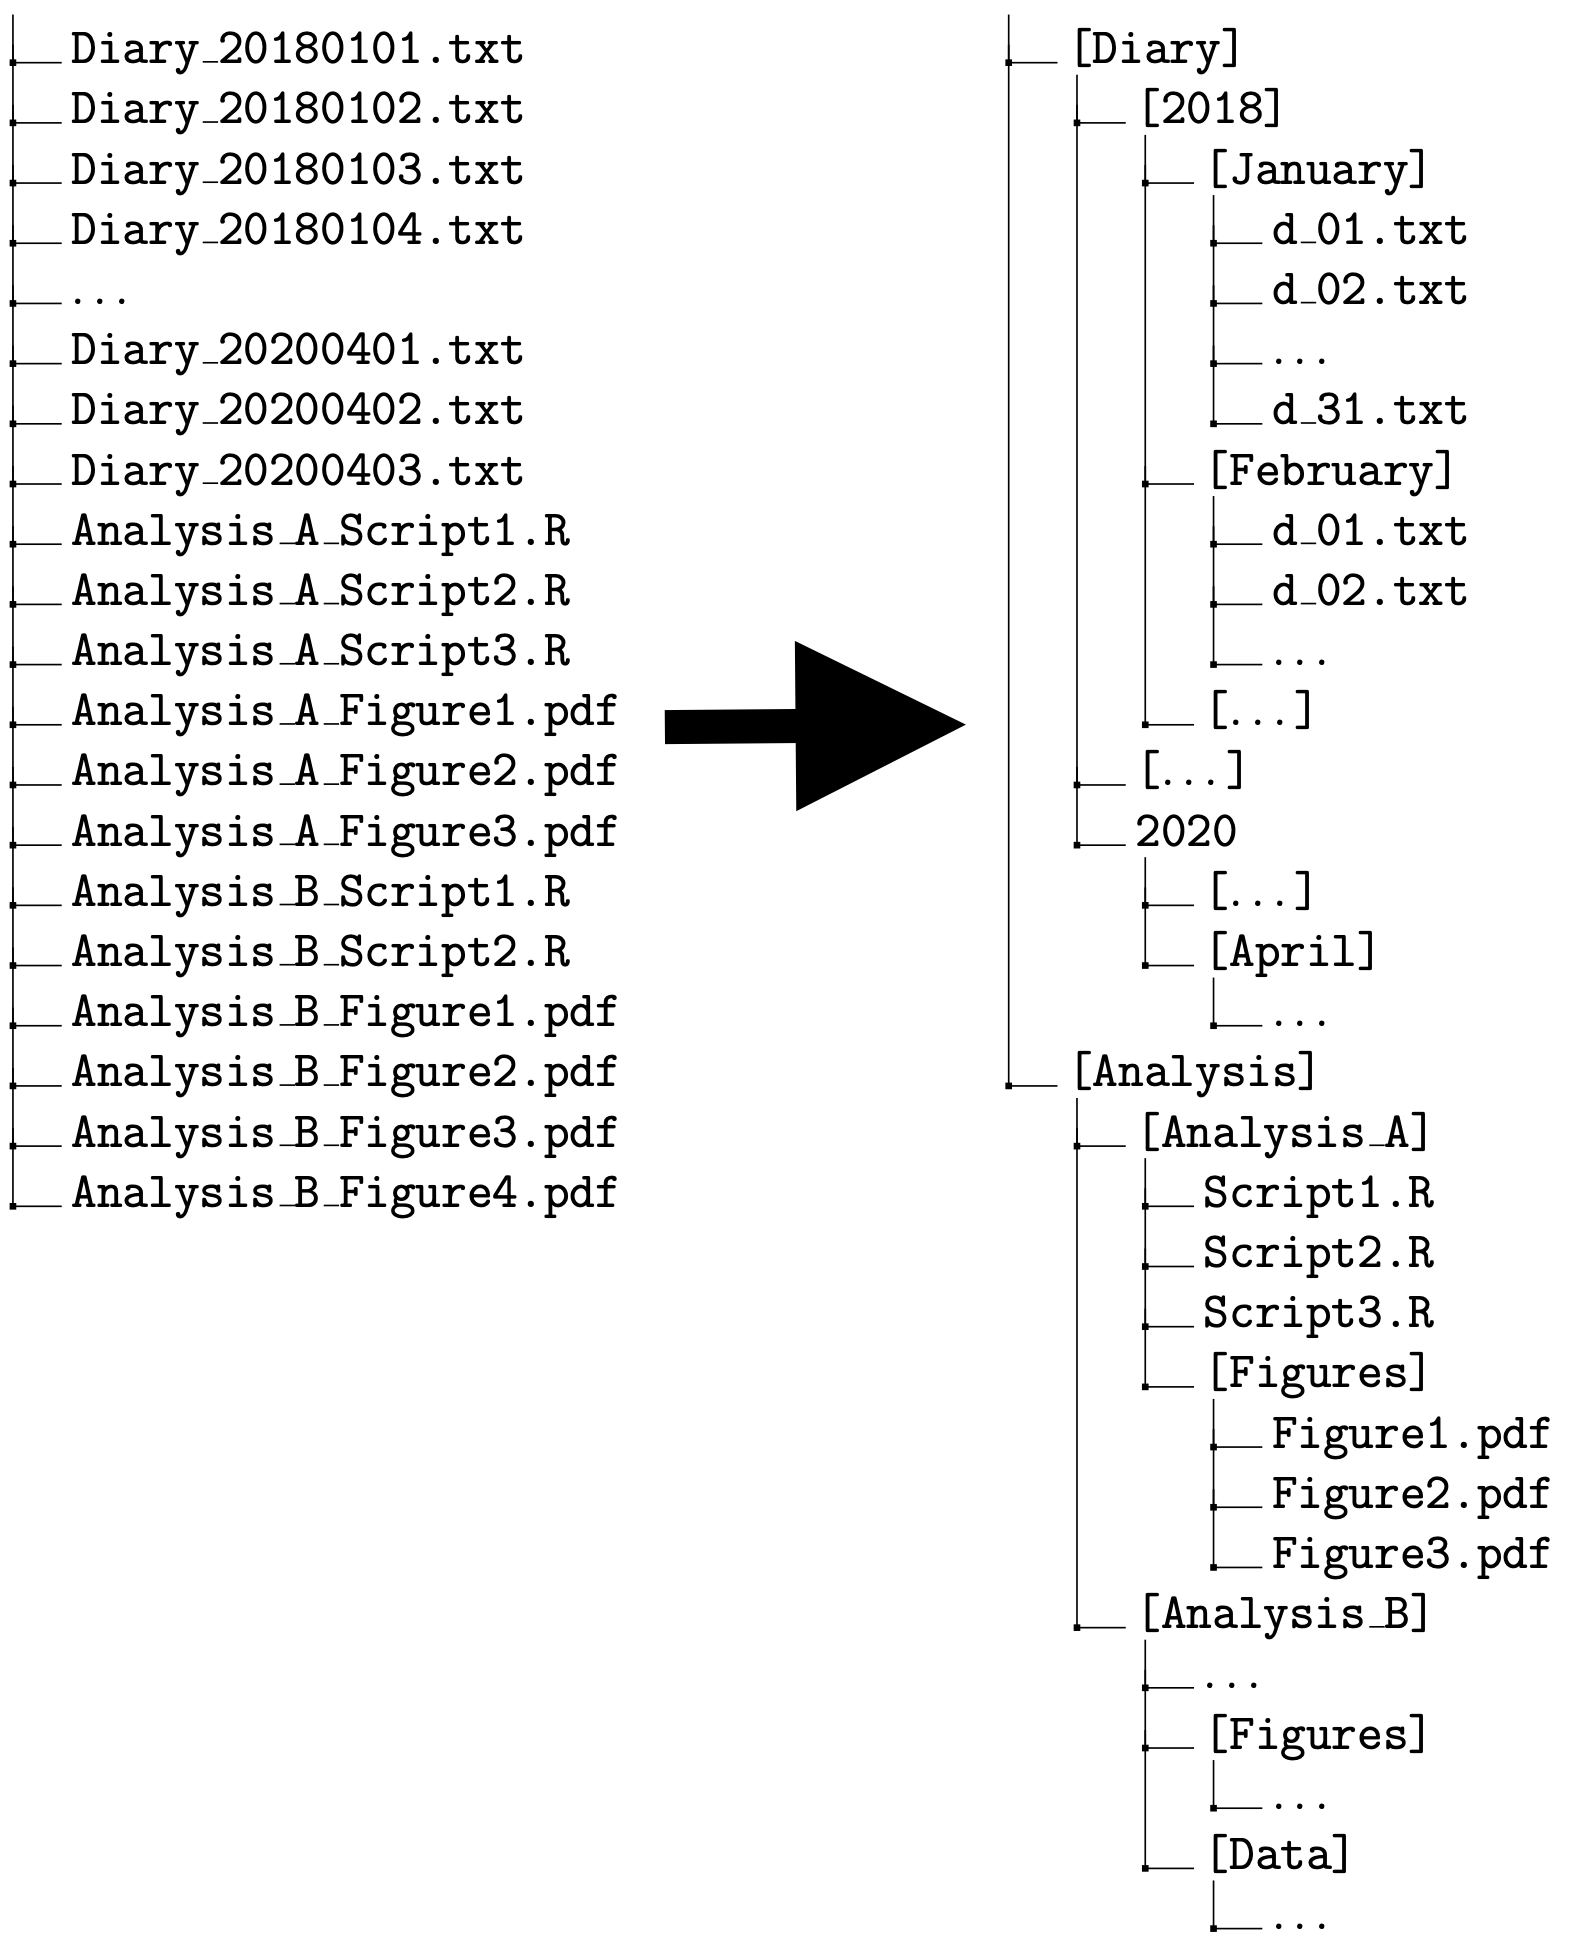
\includegraphics[width=0.75\textwidth,height=\textheight]{./Figs/Rbasic/Filesystem1.png}

}

\caption{\label{fig-rbasic_filesystem}ファイルシステムの例}

\end{figure}

 図の左側にある Diary\_YYYYMMDD.txt
がYYYY年MM月DD日の日記を保存したテキストファイルだとしよう\footnote{ファイル名拡張子が
  ``.txt'' のファイルを「テキストファイル」と呼ぶ。}。
3年間毎日日記を書くと、それだけでファイル数は1000個以上になる。また、Analysis\_blahblah.R
はRスクリプトである\footnote{ファイル名拡張子が ``.R'' または ``.r''
  のファイルを「Rスクリプト」と呼ぶ。}。Rスクリプトファイルも複数ある。さらに、上の図には表示されていないが、自分で作ったファイル以外に、OSやソフトウェア(アプリ)を構成するファイルもドライブ内に保存されているだろう。これらのファイルが整理されずに1つの場所にまとめて置いてあるとしよう(上の図の左側の状態)。そうすると、特定のファイルを開いたり、それぞれのファイルがどのような目的で存在するのかを把握したりするのに少なからぬ労を要する。

 単に面倒なだけならいい(私たちは面倒なことが大嫌いなので良くないと考える)が、ファイルの置き場が1つだけだと解決できない問題がある。それは、ファイル名の重複が許されないということだ。世の中には、特定の目的のために使われる「お決まりのファイル名」というものがある。例えば、GitHubにレポジトリを追加するときは、そのレポジトリについて説明する
\texttt{README.md}
というファイルを作ることになっている。しかし、名前が同じだとファイルが区別できないので、同じ場所にまったく同じ名前のファイルを2つ置くことはできない。したがって、ドライブ内にファイル置き場が1つしかないとなると、1つのパソコンで作れる
README.md は1つだけということになってしまい、困ってしまう。

 そこで、多くのOSではファイルをグループ化して管理するという方法が採用されている。このグループのことを「\textbf{フォルダ
(folder)}」または「\textbf{ディレクトリ
(directory)}」と呼ぶ\footnote{本書では、フォルダとディレクトリを同義語として扱う。}。

 上の図の右側は、ファイルをフォルダに分けた様子を表している。
日記のテキストファイルに注目すると、まず、``Diary''
という名前のフォルダがあり、Diary フォルダの中に年ごとのフォルダ
``2018'', ``2019'', ``2020''
というフォルダがある。それぞれの年のフォルダの中には、``January'',
``February'', \(\dots\), ``December''
という月ごとのフォルダがある。そして、それぞれの月のフォルダの中に、日付がファイル名になったテキストファイルd\_01.txt,
d\_02.txt, \(\dots\)
が保存されている。この例からわかるように、フォルダの中にフォルダを作り、そのフォルダの中にフォルダを作り
\(\cdots\)
ということができるので、フォルダを入れ子にした階層構造を利用してファイルを管理することができる。

 ファイルを階層化して管理する場合、フォルダの構造と場所を把握することが必要になる。そのために使われるのが\textbf{パス
(path)}
である。パスは、コンピュータ内の住所のようなものだと考えればよい。例えば、``Diary''
フォルダ内の ``2018'' フォルダ内の ``January'' フォルダ内の
``d\_01.txt''
というファイルのパスは、\texttt{Diary/2018/January/d\_01.txt}
である。この例からわかるように、パスにはフォルダ名やファイル名がそのまま使われる。そして、フォルダの「中」であることは、\texttt{/}
(スラッシュ)記号によって表される。例えば、\texttt{Diary/}
の部分が、Diary フォルダの中であることを示す。ただし、Windows では
\texttt{/} の代わりに
\texttt{\textbackslash{}}(バックスラッシュ)または \texttt{¥}(円記号;
日本語環境の場合)が使われる\footnote{これ以降、原則としてパスの表記には
  \texttt{/} を使うので、Windowsユーザはご注意を。}。
\texttt{Diary/2018/January/d\_01.txt} と
\texttt{Diary/2018/February/d\_01.txt} は、ファイル名だけを見れば同じ
d\_01.txt
だが、パスが異なるので異なるファイルとして認識され、1つのドライブ内に共存することができる。

 しかし、上に書いたパスは、``Diary''
フォルダがどこにあるかを指定していないので完全ではない。パソコンがファイルの場所を正しく把握するには、``Diary''
フォルダの置き場所がどこかという情報も必要である。

 パソコン内でパスの起点になる場所は、OSによって異なる。Linux
やmacOSでは、パスの起点となる最上位フォルダは \texttt{/}
であり、多くのWindows機では \texttt{C:\textbackslash{}}
(Cドライブと呼ばれる)である\footnote{かつては、AドライブとBドライブがフロッビーディスクに使われていた。その名残でCドライブが使われている。}。また、多くのOSでは、ドライブ内に「ホーム
(HOME)」と呼ばれる特別なフォルダがあらかじめ用意されており、通常はホームフォルダの中に自分で作ったファイルを保存する。ただし、ホームフォルダの名前は
``HOME''
ではないので注意が必要である。例えば、macOSではユーザ名がホームフォルダの名前である。例えば、ユーザ名が
yukiなら \texttt{/Users/yuki/} が、ユーザ名が jaehyunsong なら
\texttt{/Users/jaehyunsong/} がホームフォルダのパスである。パスの先頭に
\texttt{/} がついており、最上位フォルダの中の ``Users''
フォルダの中にユーザ名でホームフォルダが作られれている。

 ホームフォルダの中に \texttt{Diary}
フォルダがあるとすると、2018年1月1日の日記までのパスは、
\texttt{/Users/jaehyunsong/Diary/2018/January/d\_01.txt}
である。このように、ドライブ内の起点から書いた完全なパスを
\textbf{絶対パス (absolute path)} または \textbf{フルパス (full path)}
と呼ぶ。絶対パスを使えば、コンピュータ内の特定のファイルを一意に示すことができる。
絶対パスにホームディレクトリが含まれている場合には、ホームディレクトリまでのパスを省略して
\texttt{\$\{HOME\}/} または \texttt{\textasciitilde{}/}
と書くことができる。よって、上の絶対パスは、\texttt{\textasciitilde{}/Diary/2018/January/d\_01.txt}
と書くことができる。この書き方を使えば、パスを書き換えることなく共同研究者とファイルを共有することが可能になる(もちろん、ホームフォルダ以下の構造を揃える必要がある)。

 自分が作業・操作の対象としているフォルダは、\textbf{作業フォルダ}
(working directory; current directory)
と呼ばれる\footnote{Rでは、\texttt{getwd()}
  で現在の作業フォルダを確認できる。また、\texttt{setwd()}
  で作業フォルダを変更できる。例えば、\texttt{setwd("\textasciitilde{}/Diary")}
  とすれば、ホームフォルダ内の Diary
  フォルダを作業フォルダに指定できる。しかし、これらの関数は基本的には使わない。この後説明するとおり、RStudio
  のプロジェクト機能の使用を推奨する。}。絶対パスの代わりに、作業フォルダから見た\textbf{相対パス
(relative path)}を使うこともできる。例えば、現在の作業フォルダが
\texttt{\textasciitilde{}/Diary/2018/}
だとすると、2018年1月1日の日記への相対パスは、\texttt{Januaray/d\_01.txt}
と書ける。
作業フォルダを指定していることを明示したい場合(プログラムを実行する場合にはこれが必要なことがある)には、
\texttt{./Januaray/d\_01.txt} と書く。つまり、\texttt{./}
が作業フォルダを示す。 また、作業フォルダよりも階層が1つ上のフォルダ(親
{[}parent{]} フォルダと呼ぶ)には、\texttt{../}
でアクセスでききる。例えば、、現在の作業フォルダが
\texttt{\textasciitilde{}/Diary/2018/} だとすると、\texttt{../} は
\texttt{\textasciitilde{}/Diary/} なので、
20\textbf{20}年1月1日の日記への相対パスは \texttt{../2020/Januaray/d\_01.txt}
と書くことができる。

 相対パスの利点は、

\begin{enumerate}
\def\labelenumi{\arabic{enumi}.}
\tightlist
\item
  絶対パスより短い
\item
  同じ構造を再利用できる
\end{enumerate}

ということである。1は自明だろう。2は、例えば日記の一覧を作るためのプログラムを書き、それを「年」を表すフォルダに保存すれば、1つひとつの日記に毎年同じ相対パスでアクセスできる(ただし、2月29日は除く)ので、毎年同じプログラムを利用できて便利である。絶対パスを使うと、「年」の部分を毎年書き換えなければいけない。

 絶対パスと相対パスは、目的に応じて使い分けることが必要である。

\hypertarget{sec-rbasic_project}{%
\section{「プロジェクト」のすゝめ}\label{sec-rbasic_project}}

 Rを使ったプログラミングやデータ分析を進めていくと、自分が書いたRスクリプトや作成した図表だけでなく、
Rが自動的に生成するファイルもどんどん溜まる。そう遠くない将来、ドライブ内のファイル数が数万に達しても不思議ではない。効率よくプログラミングを行うために、ファイルの管理方法を明確にしておいたほうが良い。そのためには、フォルダの階層化を利用してファイルを管理することが必要である。

 しかし、フォルダによる階層化を導入すればファイルの管理が楽になるかというと、必ずしもそうとは限らない。かえって不便になる部分もある。前の節で見たとおり、フォルダを階層化すると、絶対パスが長く(複雑に)なる。ファイルを階層化によって整理したとしても、ファイルを利用するたびに長い絶対パスの入力が必要なら、ファイル管理の効率が上がったとは言えないだろう。

 Rを使う場合にファイル管理の効率化を助けてくれるのが、RStudio
の「プロジェクト」機能である。

\hypertarget{ux30d7ux30edux30b8ux30a7ux30afux30c8}{%
\subsection{プロジェクト}\label{ux30d7ux30edux30b8ux30a7ux30afux30c8}}

 Rの既定(デフォルト)の作業フォルダはホームフォルダある。分析に使うデータが、ホームフォルダの中の
\texttt{Documents} フォルダの中の \texttt{R} フォルダの中の
\texttt{Analysis1} フォルダ内の \texttt{Data} フォルダにある
\texttt{data.csv}
だとしたら、このファイルにアクセスするためには、\texttt{"Documents/R/Analysis1/Data/data.csv"}と入力する必要がある\footnote{Rでパスを指定するときは、パスを引用符で囲む。引用符は、\texttt{""}
  でも \texttt{\textquotesingle{}\textquotesingle{}} でも良い。} \(^,\)
\footnote{\texttt{file.path()}
  を使って、\texttt{file.path("Documents",\ "R",\ "Analysis",\ "Data",\ "data.csv")}
  と書くこともできる。この書き方の利点は、\texttt{/},
  \texttt{\textbackslash{}}, \texttt{¥}
  を環境に応じて使い分けてくれることである。}。新たに作った図を
``histogram.pdf'' という名前でホームフォルダの中の \texttt{Documents}
フォルダの中の \texttt{R} フォルダの中の \texttt{Analysis1} フォルダ内の
\texttt{Figures}
というフォルダに保存するためには、\texttt{"Documents/R/Analysis1/Figures/historam.pdf"}と入力する必要がある。どちらもかなり面倒で、効率が悪い。

 しかし、作業フォルダが、\texttt{\textasciitilde{}/Documents/R/Analysis1/}
だとすれば、相対パスにより、\texttt{"Data/data.csv"}
や\texttt{"Figures/historam.pdf"}
だけで済む。よって、作業フォルダを明示的に指定すればいいわけだが、作業フォルダを毎回指定するのも面倒だ。

 そこで利用できるのが、RStudio のプロジェクト機能である。
プロジェクトとは、特定のフォルダを作業フォルダに設定し、すべての作業をそのフォルダと下位フォルダのみに限定してくれる機能である\footnote{何らかの事情により、作業ディレクトリ以外のフォルダにアクセスすることが必要なときは、絶対パスを使えば良い。}。プロジェクト機能さえ使えば、ユーザが意識しなくても、ユーザが書いたコード、保存したデータ、作成した図などが作業フォルダ内に集約され、管理が楽になる。

 では、ここからプロジェクトの作り方を説明しよう。

\begin{enumerate}
\def\labelenumi{\arabic{enumi}.}
\item
  まずはRStudio を起動する。
\item
  RStudio が起動したら、``File'' から ``New Project'' を選択する。
\end{enumerate}

\begin{figure}

{\centering 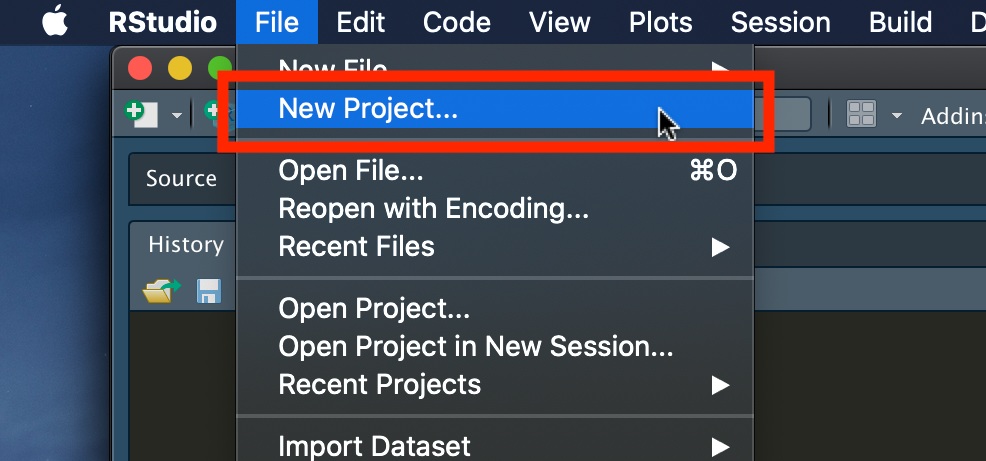
\includegraphics[width=0.75\textwidth,height=\textheight]{./Figs/Rbasic/Project1.png}

}

\caption{\label{fig-rbasic_project1}FileからNew Project\ldots{}}

\end{figure}

\begin{enumerate}
\def\labelenumi{\arabic{enumi}.}
\setcounter{enumi}{2}
\tightlist
\item
  下の画面が表示されたら、 ``New Directory''
  を選択する。ただし、既存のフォルダを利用したい場合は、 ``Existing
  Directory'' を選ぶ。
\end{enumerate}

\begin{figure}

{\centering 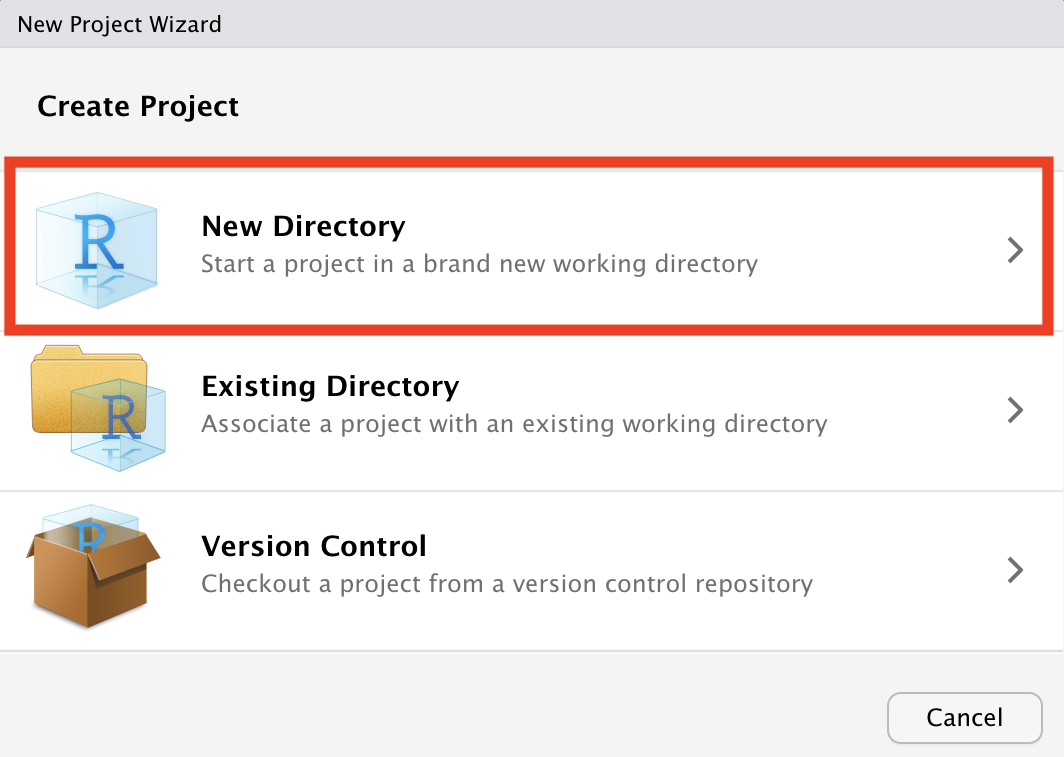
\includegraphics[width=0.75\textwidth,height=\textheight]{./Figs/Rbasic/Project2.png}

}

\caption{\label{fig-rbasic_project2}New Directoryを選択}

\end{figure}

\begin{enumerate}
\def\labelenumi{\arabic{enumi}.}
\setcounter{enumi}{3}
\tightlist
\item
  下の画面が表示されたら、``New Project'' を選択する。
\end{enumerate}

\begin{itemize}
\tightlist
\item
  前の手順で ``Existing Directory''
  を選択した場合、この画面は表示されない。
\end{itemize}

\begin{figure}

{\centering 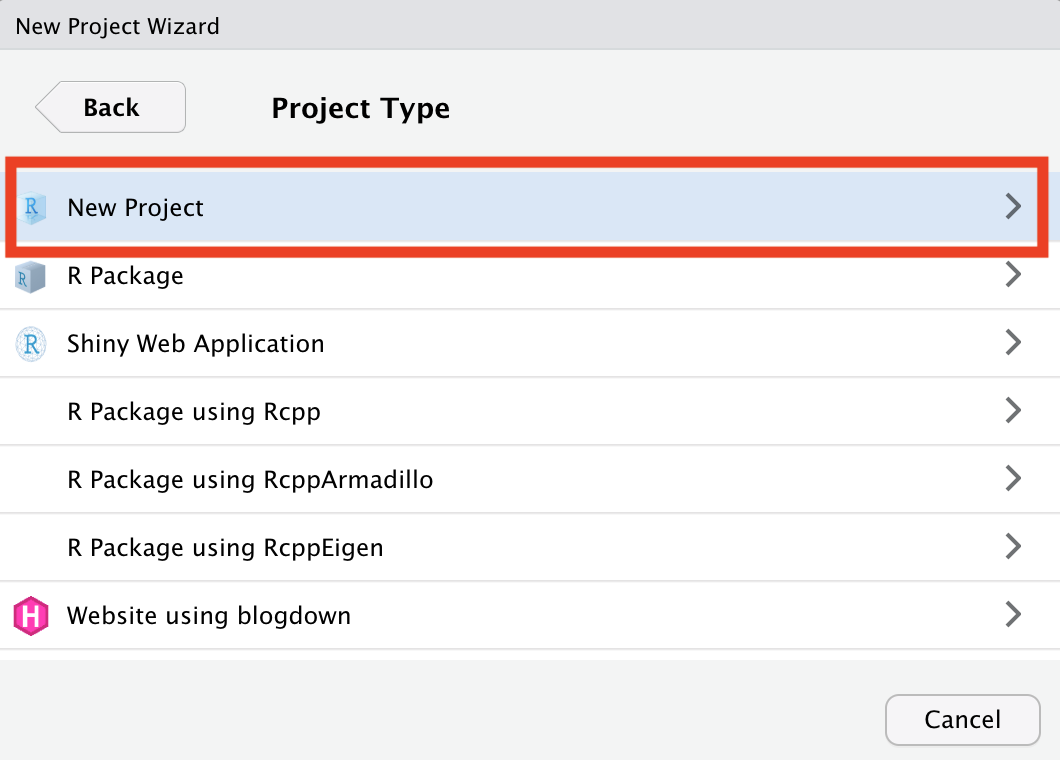
\includegraphics[width=0.75\textwidth,height=\textheight]{./Figs/Rbasic/Project3.png}

}

\caption{\label{fig-rbasic_project3}New Projectを選択}

\end{figure}

\begin{enumerate}
\def\labelenumi{\arabic{enumi}.}
\setcounter{enumi}{4}
\tightlist
\item
  下の画面が表示されたら、``Directory name:''
  にプロジェクト名を入力する。これがフォルダ名になるので、\textbf{半角英数字のみ}の
  名前を付ける。ここでは第4章のコードということで、``Ch04''
  にした。統計学の授業用プロジェクトなら
  ``statistics''、計量政治学の授業なら ``quant\_methods\_ps''
  などの名前を付ければ良いだろう。英語が嫌なら ``tokeigaku''
  のようにすれば良い。また、``Create project as subdirectory of:''
  では、プロジェクトのフォルダをどのフォルダの中に設置するかを指定する。
  ``Browse\ldots{}'' をクリックし、親フォルダを選ぶ。ここでは
  \texttt{\textasciitilde{}/Dropbox/RStudy}
  にプロジェクトのフォルダを入れることにする。ここまでできたら、``Create
  Project'' をクリックする。
\end{enumerate}

\begin{itemize}
\tightlist
\item
  手順3で ``Existing Directory''
  を選んだ場合、プロジェクトのフォルダとして使う既存フォルダを選択する画面が表示される。
\end{itemize}

\begin{figure}

{\centering 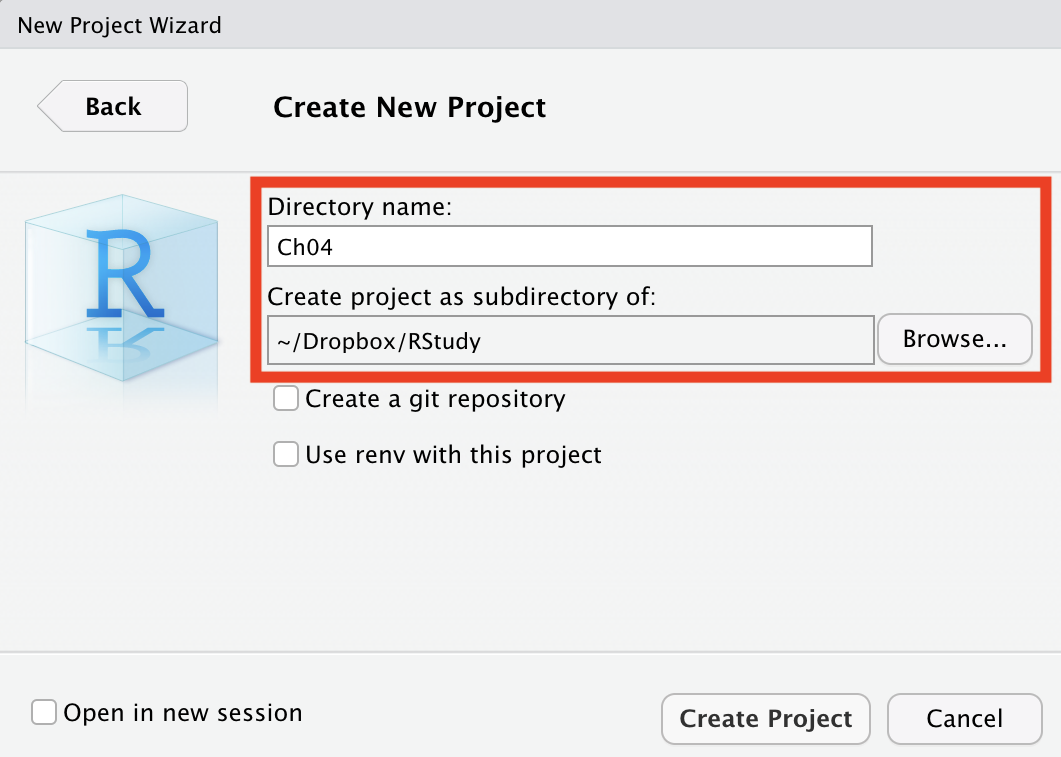
\includegraphics[width=0.75\textwidth,height=\textheight]{./Figs/Rbasic/Project4.png}

}

\caption{\label{fig-rbasic_project4}プロジェクト名と保存場所の指定}

\end{figure}

\begin{enumerate}
\def\labelenumi{\arabic{enumi}.}
\setcounter{enumi}{5}
\tightlist
\item
  以上の手順でプロジェクトができる。RStudio
  右上に、プロジェクト名が表示されているはずだ。 また、Console に
  \texttt{getwd()}
  と入力すると、プロジェクトまでの絶対パスが表示される。
\end{enumerate}

 念のため、Finder(Macの場合)やエクスプローラー (Windows
の場合)で、指定した場所にプロジェクトのフォルダ(上の例では
\texttt{Ch04})が生成されていることを確認しよう。
プロジェクトフォルダを開いてみると、\texttt{Ch04.Rproj}
というファイルが生成されていることがわかる(下の図)。

\begin{figure}

{\centering 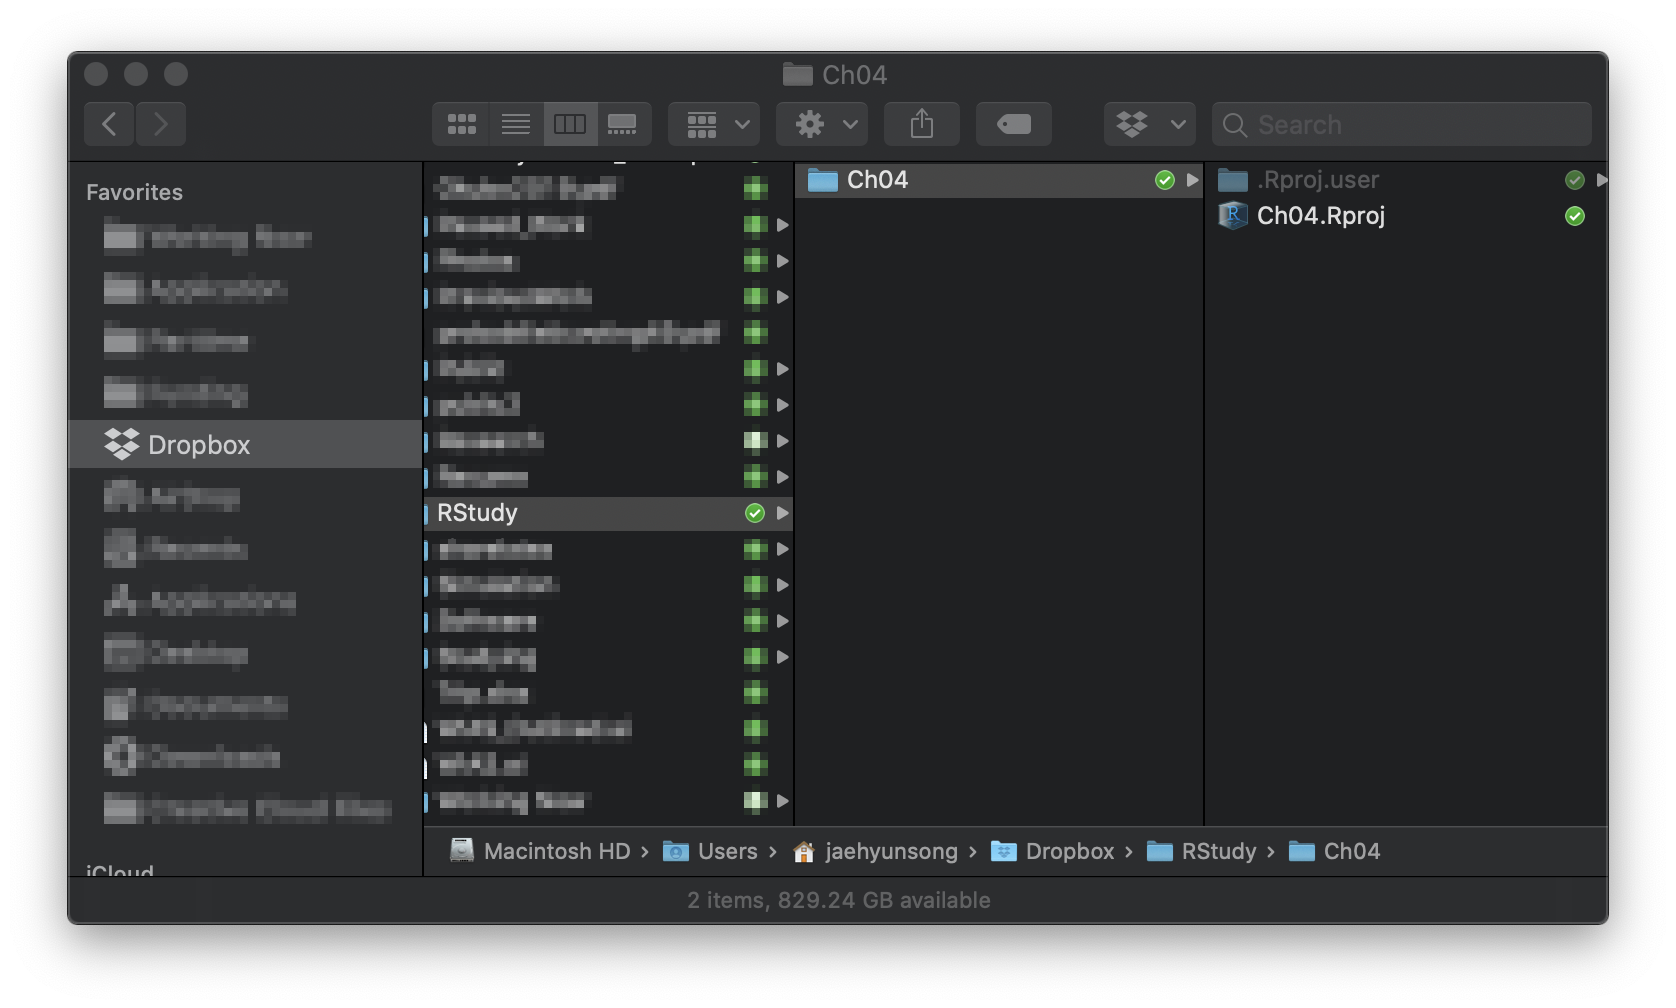
\includegraphics[width=0.75\textwidth,height=\textheight]{./Figs/Rbasic/Project5.png}

}

\caption{\label{fig-rbasic_project5}プロジェクトの確認}

\end{figure}

 \texttt{Ch04} プロジェクトを開くには、この\texttt{Ch04.Rproj}
ファイルをダブルクリックすれば良い。RStudio
が起動していない場合でも、指定のプロジェクトを開いた状態でRStudio
が起ち上がる。

 RStudio 右上の表示が ``Project: (None)''
となっているときは、プロジェクトが開かれていない。 \textbf{RStudio
を使う場合には、必ず右上の表示を見て、プロジェクトが開かれていることを確認しよう。}
プロジェクトが開かれていない場合には、既存のプロジェクトを開くか、新たばプロジェクトを作ろう。

\hypertarget{sec-rbasic_calc}{%
\section{電卓としてのR}\label{sec-rbasic_calc}}

 前置きが長かったが、ここからはRを使っていこう。まず、新しい R Script
を開くために、Cmd/Ctrl + Shift + N を入力する\footnote{Mac では、command
  + shift + N、Windows では Ctrl + Shift + N のショートカットが使える。}(``File''
メニューから ``New File'' - ``R Script'' を選んでも良い)。すると、
左上の Source Pane に ``Untitled1'' というタブが登場し、その pane
上でコードが入力できるようになる。ここで \texttt{3\ +\ 3}
と入力し、その行にカーソルを留めたまま command + return(Mac)または
Ctrl + Enter を押してみよう。command + return というのは、command
キーを押したまま、return キーも押すという意味である。

\begin{figure}

{\centering 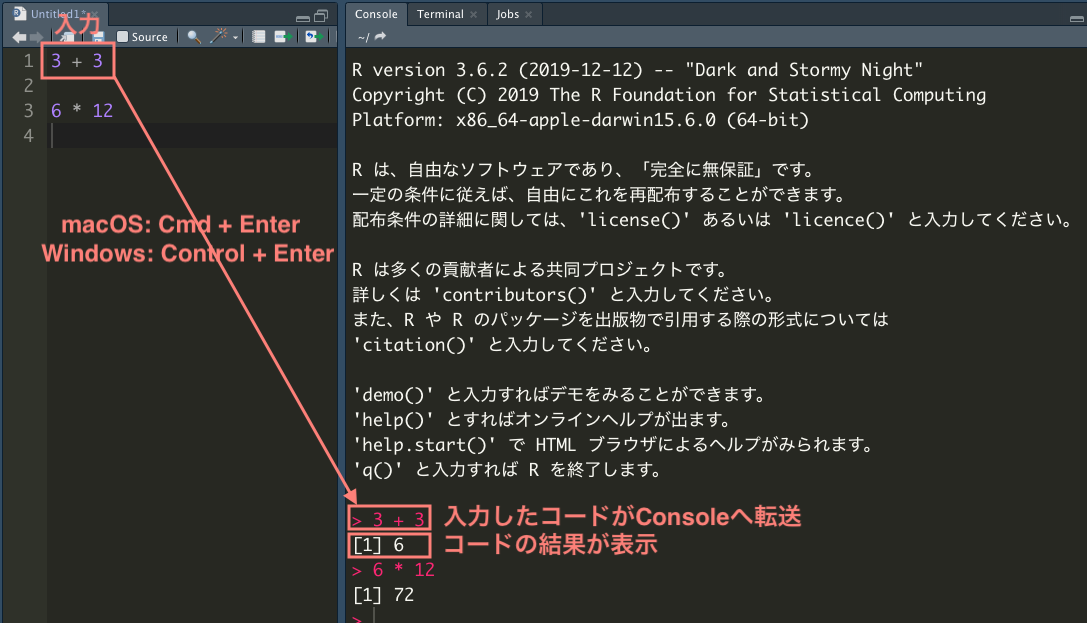
\includegraphics[width=0.75\textwidth,height=\textheight]{./Figs/Rbasic/InputCode1.png}

}

\caption{\label{fig-rbasic_inputcode1}コード入力の例}

\end{figure}

 Source ペイン (Untitled1) に入力したコードが
Console(本書の説明どおりにカスタマイズしていれば、RStudio
内の右上画面)に転送され、計算結果が表示される。Rのコードは Console
に直接打ち込むこともできるが、Sourceペインで入力してから Console
に転送する方法が基本である\footnote{電卓として使う程度なら、Consoleに直接入力してもかまわない。}。
Source
ペインの内容をファイルに保存すれば、後でもう1度同じコードを実行したり、コードを他のプロジェクトで再利用することができるようになる。先ほど
\texttt{3\ +\ 3} を入力した画面にカーソルを合わせ、Cmd/Ctrl + S
を押してみよう。ファイルの保存を促されるので、ファイル名をつけて保存しよう。このとき、\textbf{.R
というファイル名拡張子を付ける}。これにより、ファイルが\textbf{Rスクリプト}として認識される。例えば、``practice01.R''
という名前をつけて保存しよう。Sourceペインの上部に表示されるタブの名前が、``Untitled1''
から ``practice01.R'' に変わることが確認できるはずだ。

 以下にRで計算する例を示すので、コードを \texttt{practice01.R}
に入力し、command + return (Ctrl + Enter) で Console
に送り、実行結果を確認しよう。背景が灰色になっている部分に示されているのが、Rのコマンドである。ただし、\textbf{\texttt{\#\#}から始まる部分は計算結果である}。また、コードブロックのうち、
\texttt{\#}(ハッシュ記号)で始まる部分はコメントであり、Rで評価(計算)されない。コメントの使い方
については第\ref{sec-rmarkdown}章で詳しく解説する。

\hypertarget{ux7b97ux8853ux6f14ux7b97ux5b50}{%
\subsection{算術演算子}\label{ux7b97ux8853ux6f14ux7b97ux5b50}}

 まずは、簡単な足し算と掛け算を実行してみよう。

\begin{Shaded}
\begin{Highlighting}[numbers=left,,]
\DecValTok{3} \SpecialCharTok{+} \DecValTok{3}
\end{Highlighting}
\end{Shaded}

\begin{verbatim}
[1] 6
\end{verbatim}

\begin{Shaded}
\begin{Highlighting}[numbers=left,,]
\DecValTok{8} \SpecialCharTok{*} \DecValTok{2}
\end{Highlighting}
\end{Shaded}

\begin{verbatim}
[1] 16
\end{verbatim}

これ以外の基本的な演算は以下のとおりである。

\begin{longtable}[]{@{}llll@{}}
\toprule
演算子 & 意味 & 例 & 結果 \\
\midrule
\endhead
\texttt{+} & 和 & \texttt{2\ +\ 5} & 7 \\
\texttt{-} & 差 & \texttt{2\ -\ 8} & -6 \\
\texttt{*} & 積 & \texttt{7\ *\ 3} & 21 \\
\texttt{/} & 商 & \texttt{16\ /\ 5} & 3.2 \\
\texttt{\^{}}、\texttt{**} & 累乗(べき乗) &
\texttt{2\^{}3}または\texttt{2\ **\ 3} & 8 \\
\texttt{\%\%} & 剰余 (モジュロ) & \texttt{18\ \%\%\ 7} & 4 \\
\texttt{\%/\%} & 整数商 & \texttt{18\ \%/\%\ 7} & 2 \\
\bottomrule
\end{longtable}

\hypertarget{ux8ad6ux7406ux6f14ux7b97ux5b50}{%
\subsection{論理演算子}\label{ux8ad6ux7406ux6f14ux7b97ux5b50}}

 論理演算子とは、入力した式が真か偽かを判定する演算子である。返り値(戻り値)は
\texttt{TRUE}(真の場合)または
\texttt{FALSE}(偽の場合)のいずれかとなる。たとえば、「3 \textgreater{}
2」は真なので、\texttt{TRUE} が返される。しかし、「2 + 3 =
1」は偽なので、\texttt{FALSE}が返される。実際にやってみよう。

\begin{Shaded}
\begin{Highlighting}[numbers=left,,]
\DecValTok{3} \SpecialCharTok{\textgreater{}} \DecValTok{2}
\end{Highlighting}
\end{Shaded}

\begin{verbatim}
[1] TRUE
\end{verbatim}

\begin{Shaded}
\begin{Highlighting}[numbers=left,,]
\DecValTok{2} \SpecialCharTok{+} \DecValTok{3} \SpecialCharTok{==} \DecValTok{1}
\end{Highlighting}
\end{Shaded}

\begin{verbatim}
[1] FALSE
\end{verbatim}

 このように、等しいかどうかを表す記号は \texttt{=} ではなく
\texttt{==}(二重等号)なので注意されたい。

 論理演算子にも、いくつかの種類がある。

\begin{longtable}[]{@{}lllll@{}}
\toprule
& 演算子 & 意味 & 例 & 結果 \\
\midrule
\endhead
1 & \texttt{x\ \textless{}\ y} & \texttt{x}は\texttt{y}より小さい &
\texttt{3\ \textless{}\ 1} & FALSE \\
2 & \texttt{x\ \textless{}=\ y} &
\texttt{x}は\texttt{y}と等しいか、小さい & \texttt{2\ \textless{}=\ 2} &
TRUE \\
3 & \texttt{x\ \textgreater{}\ y} & \texttt{x}は\texttt{y}より大きい &
\texttt{6\ \textgreater{}\ 5} & TRUE \\
4 & \texttt{x\ \textgreater{}=\ y} &
\texttt{x}は\texttt{y}と等しいか、大きい &
\texttt{4\ \textgreater{}=\ 5} & FALSE \\
5 & \texttt{x\ ==\ y} & \texttt{x}と\texttt{y}は等しい &
\texttt{(2\ +\ 3)\ ==\ (4\ +\ 1)} & TRUE \\
6 & \texttt{x\ !=\ y} & \texttt{x}と\texttt{y}は等しくない &
\texttt{((2\ *\ 3)\ +\ 1)\ !=\ (2\ *\ (3\ +\ 1))} & TRUE \\
\bottomrule
\end{longtable}

 6番目の例について少し説明する。通常の数式同様、Rも括弧\texttt{()}内の記述を優先的に計算する。したがって、\texttt{!=}左側の\texttt{((2\ *\ 3)\ +\ 1)}
は \texttt{6\ +\ 1\ =\ 7} であり、右側の \texttt{(2\ *\ (3\ +\ 1))} は
\texttt{2\ *\ 4\ =\ 8} である。したがって、\texttt{7\ !=\ 8}
が判定対象となり、\texttt{TRUE}が返される。\texttt{!}
記号は、「否定」を表すために使われるもので、\texttt{!=}
は左右が等しくないときに \texttt{TRUE} を返す

 上に挙げた論理演算子は基本的に数字を対象に使うが、\texttt{TRUE}と\texttt{FALSE}
を対象に使うものもある。それが and を表す \texttt{\&} と or
を表す\texttt{\textbar{}} である。\texttt{\&}
は、\texttt{\&} を挟む左右の両側が \texttt{TRUE} の場合のみ
\texttt{TRUE} を返し、\texttt{\textbar{}} は少なくとも一方が
\texttt{TRUE} なら \texttt{TRUE} を返す。

\begin{longtable}[]{@{}lllll@{}}
\toprule
& 演算子 & 意味 & 例 & 結果 \\
\midrule
\endhead
1 & \texttt{x\ \textbar{}\ y} & \texttt{x}または\texttt{y} &
\texttt{(2\ +\ 3\ ==\ 5)\ \textbar{}\ (1\ *\ 2\ ==\ 3)} & TRUE \\
2 & \texttt{x\ \&\ y} & \texttt{x}かつ\texttt{y} &
\texttt{(2\ +\ 3\ ==\ 5)\ \&\ (1\ *\ 2\ ==\ 3)} & FALSE \\
\bottomrule
\end{longtable}

 1番の例では、\texttt{\textbar{}}の左側は\texttt{(2\ +\ 3\ ==\ 5)}であり、\texttt{TRUE}
である。一方、右側の\texttt{(1\ *\ 2\ ==\ 3)} は \texttt{FALSE}
だ。判定対象は\texttt{TRUE\ \textbar{}\ FALSE} となり、\texttt{TRUE}
が返される。 2番目の例は \texttt{TRUE\ \&\ FALSE} なので、返り値は
\texttt{FALSE} になる。

\hypertarget{sec-rbasic_input}{%
\section{格納とオブジェクトの作成}\label{sec-rbasic_input}}

\begin{itemize}
\tightlist
\item
  まず、\texttt{123454321\ *\ 2} を計算しよう。
\item
  次に、\texttt{123454321\ *\ 3} を計算しよう。
\item
  最後に、\texttt{123454321\ *\ 4} を計算しよう。
\end{itemize}

 これらの計算は簡単にできるだろう。しかし、\texttt{123454321}を3回入力するのが面倒だっただろう\footnote{反復作業が面倒だと感じるほどプログラミングが上達しやすい。}。\texttt{123454321}という数字を\texttt{x}とか\texttt{a}に代入し、数字の代わりに
\texttt{x} や \texttt{a}
が使えるなら、上の計算は楽になる。ここではその方法を説明する。

 \texttt{x}というものに\texttt{123454321}という数字を入れるには、\texttt{\textless{}-}
という演算子を使う。この演算子により、\texttt{x}という名のもの
(オブジェクト)に\texttt{123454321}という数字を代入することができる。ここでは「代入」という表現を使ったが\footnote{代入の代わりに「付値」と言うこともある。}、\texttt{\textless{}-}の役割は代入よりも広いので、これからは「格納」という表現を使う。

 \texttt{\textless{}-} は、\texttt{\textless{}} と\texttt{-}
という\textbf{2つの記号をスペースなしで}入力することで作ることができる。
RStudioでは、 option + \texttt{-} {[}マイナス, ハイフン{]} (macOS 場合)
または Alt + \texttt{-} (Windows の場合)で、\texttt{\textless{}-}
が入力できる。その際、演算子の前後に半角スペースが1つずつ挿入されるので、\textbf{このショートカットは必ず使うべき}である。

 Rを起動した時点では、\texttt{x}
というオブジェクトは存在しない。RStudio 右下のペインにある Environment
タブを開くと、現時点では何も表示されていないはずだ。しかし、\texttt{x}
に何かを格納することで、\texttt{x} というオブジェクトができる。 実際に
\texttt{x}に、\texttt{123454321}を格納してみよう。

\begin{Shaded}
\begin{Highlighting}[numbers=left,,]
\NormalTok{x }\OtherTok{\textless{}{-}} \DecValTok{123454321}  \CommentTok{\# xに123454321を格納}
\end{Highlighting}
\end{Shaded}

Environment タブに、\texttt{x}
が登場し、格納した数字が右側に表示されていることが確認できるだろう。

 オブジェクトの中身は、オブジェクト名をそのまま入力することで表示できる。

\begin{Shaded}
\begin{Highlighting}[numbers=left,,]
\NormalTok{x}
\end{Highlighting}
\end{Shaded}

\begin{verbatim}
[1] 123454321
\end{verbatim}

 \texttt{print(x)}
でも同じ結果が得られるが、タイプする文字数を減らしたいので
\texttt{x}のみにする。ただし、状況やオブジェクトの型(型については後で詳しく説明する)によっては、\texttt{print()}
を表示しないと中身が表示されない場合もあるので、R Markdown
ファイルで論文などを作成していて、結果を確実に表示したい場合には
\texttt{print(x)} とするほうが安全である。

 ちなみに、格納と同時にそのオブジェクトの中身を表示することもできる。そのためには、格納コマンド全体を\texttt{()}
で囲む。例えば、次のようにする。

\begin{Shaded}
\begin{Highlighting}[numbers=left,,]
\NormalTok{(y }\OtherTok{\textless{}{-}} \DecValTok{2}\NormalTok{)  }\CommentTok{\# yに2を格納し、中身を表示}
\end{Highlighting}
\end{Shaded}

\begin{verbatim}
[1] 2
\end{verbatim}

 値が格納されたオブジェクトは計算に利用できるので、先ほどの計算は、次のようにできる。

\begin{Shaded}
\begin{Highlighting}[numbers=left,,]
\NormalTok{x }\SpecialCharTok{*} \DecValTok{2}
\end{Highlighting}
\end{Shaded}

\begin{verbatim}
[1] 246908642
\end{verbatim}

\begin{Shaded}
\begin{Highlighting}[numbers=left,,]
\NormalTok{x }\SpecialCharTok{*} \DecValTok{3}
\end{Highlighting}
\end{Shaded}

\begin{verbatim}
[1] 370362963
\end{verbatim}

\begin{Shaded}
\begin{Highlighting}[numbers=left,,]
\NormalTok{x }\SpecialCharTok{*} \DecValTok{4}
\end{Highlighting}
\end{Shaded}

\begin{verbatim}
[1] 493817284
\end{verbatim}

 文字列を格納することもできる。ただし、文字列は必ず \texttt{""} か
\texttt{\textquotesingle{}\textquotesingle{}} で囲む必要がある。

\begin{Shaded}
\begin{Highlighting}[numbers=left,,]
\NormalTok{x }\OtherTok{\textless{}{-}} \StringTok{"猫の恋 やむとき閨の 朧月(芭蕉)"}
\NormalTok{x}
\end{Highlighting}
\end{Shaded}

\begin{verbatim}
[1] "猫の恋 やむとき閨の 朧月(芭蕉)"
\end{verbatim}

 オブジェクトに格納できるのは1つの数値や文字列だけではない。複数の数値や文字列を格納することもできる。そのためには
\texttt{c()} という関数を使う。\texttt{c()} の\textbf{c} は concatenate
または combine の頭文字で、複数の要素からベクトル (vector)
を作るのに使われる関数である。 \texttt{c()} に含む要素はカンマ
(\texttt{,}) で区切る。

\begin{Shaded}
\begin{Highlighting}[numbers=left,,]
\CommentTok{\# ある日の Lions の打順をベクトルに格納する}
\NormalTok{numeric\_vec1  }\OtherTok{\textless{}{-}} \FunctionTok{c}\NormalTok{(}\DecValTok{73}\NormalTok{, }\DecValTok{6}\NormalTok{, }\DecValTok{5}\NormalTok{, }\DecValTok{3}\NormalTok{, }\DecValTok{99}\NormalTok{, }\DecValTok{10}\NormalTok{, }\DecValTok{22}\NormalTok{, }\DecValTok{9}\NormalTok{, }\DecValTok{7}\NormalTok{)}
\NormalTok{numeric\_vec1}
\end{Highlighting}
\end{Shaded}

\begin{verbatim}
[1] 73  6  5  3 99 10 22  9  7
\end{verbatim}

 複数の文字列を格納することもできる。

\begin{Shaded}
\begin{Highlighting}[numbers=left,,]
\NormalTok{character\_vec }\OtherTok{\textless{}{-}} \FunctionTok{c}\NormalTok{(}\StringTok{\textquotesingle{}cat\textquotesingle{}}\NormalTok{, }\StringTok{\textquotesingle{}cheetah\textquotesingle{}}\NormalTok{, }\StringTok{\textquotesingle{}lion\textquotesingle{}}\NormalTok{,  }\StringTok{\textquotesingle{}tiger\textquotesingle{}}\NormalTok{)}
\NormalTok{character\_vec}
\end{Highlighting}
\end{Shaded}

\begin{verbatim}
[1] "cat"     "cheetah" "lion"    "tiger"  
\end{verbatim}

 ひとつひとつの要素を指定する代わりに、様々な方法でベクトルを作ることが可能である。
たとえば、\texttt{seq()}
関数を使うと、一連の数字からなるベクトルを作ることができる。\texttt{from}
で数列の初項を、\texttt{to} で数列の最終項を指定し、\texttt{by}
で要素間の差(第2要素は第1要素に \texttt{by} を加えた値になる
)を指定するか、\texttt{length.out}
で最終的にできるベクトルの要素の数を指定する。Rのベクトルの
\textbf{length} とは、要素の数のことなので、注意されたい。

 いくつか例を挙げる。

\begin{Shaded}
\begin{Highlighting}[numbers=left,,]
\CommentTok{\# 1から20までの整数。1:20 でも同じ}
\FunctionTok{seq}\NormalTok{(}\AttributeTok{from =}  \DecValTok{1}\NormalTok{, }\AttributeTok{to =}  \DecValTok{20}\NormalTok{, }\AttributeTok{by =} \DecValTok{1}\NormalTok{)}
\end{Highlighting}
\end{Shaded}

\begin{verbatim}
 [1]  1  2  3  4  5  6  7  8  9 10 11 12 13 14 15 16 17 18 19 20
\end{verbatim}

\begin{Shaded}
\begin{Highlighting}[numbers=left,,]
\CommentTok{\# 1から19までの奇数}
\FunctionTok{seq}\NormalTok{(}\AttributeTok{from =} \DecValTok{11}\NormalTok{, }\AttributeTok{to =}  \DecValTok{20}\NormalTok{, }\AttributeTok{by =} \DecValTok{2}\NormalTok{)}
\end{Highlighting}
\end{Shaded}

\begin{verbatim}
[1] 11 13 15 17 19
\end{verbatim}

\begin{Shaded}
\begin{Highlighting}[numbers=left,,]
\CommentTok{\# 2から20までの偶数}
\FunctionTok{seq}\NormalTok{(}\AttributeTok{from =}  \DecValTok{2}\NormalTok{, }\AttributeTok{to =}  \DecValTok{20}\NormalTok{, }\AttributeTok{by =} \DecValTok{2}\NormalTok{)}
\end{Highlighting}
\end{Shaded}

\begin{verbatim}
 [1]  2  4  6  8 10 12 14 16 18 20
\end{verbatim}

\begin{Shaded}
\begin{Highlighting}[numbers=left,,]
\CommentTok{\# 降順、間隔は5}
\FunctionTok{seq}\NormalTok{(}\AttributeTok{from =} \DecValTok{20}\NormalTok{, }\AttributeTok{to =}   \DecValTok{1}\NormalTok{, }\AttributeTok{by =} \SpecialCharTok{{-}}\DecValTok{5}\NormalTok{)}
\end{Highlighting}
\end{Shaded}

\begin{verbatim}
[1] 20 15 10  5
\end{verbatim}

\begin{Shaded}
\begin{Highlighting}[numbers=left,,]
\CommentTok{\# 最小値が1、最大値が100で、lengthが10のベクトル}
\FunctionTok{seq}\NormalTok{(}\AttributeTok{from =}  \DecValTok{1}\NormalTok{, }\AttributeTok{to =} \DecValTok{100}\NormalTok{, }\AttributeTok{length.out =} \DecValTok{10}\NormalTok{)}
\end{Highlighting}
\end{Shaded}

\begin{verbatim}
 [1]   1  12  23  34  45  56  67  78  89 100
\end{verbatim}

\begin{Shaded}
\begin{Highlighting}[numbers=left,,]
\CommentTok{\# 73から1つずつ数が小さくなるlengthが10のベクトル}
\FunctionTok{seq}\NormalTok{(}\AttributeTok{from =} \DecValTok{73}\NormalTok{, }\AttributeTok{by =} \SpecialCharTok{{-}}\DecValTok{1}\NormalTok{, }\AttributeTok{length.out =} \DecValTok{8}\NormalTok{)}
\end{Highlighting}
\end{Shaded}

\begin{verbatim}
[1] 73 72 71 70 69 68 67 66
\end{verbatim}

 このように1つの関数でも指定する内容は、\texttt{by}
になったり\texttt{length.out} になったりする。\texttt{by} や
\texttt{length.out}、\texttt{from}、\texttt{to}
などのように、関数で指定する対象になっているもののことを \textbf{仮引数
(parameter)} と呼ぶ。また、\texttt{by\ =\ 1}
の1や、\texttt{length.out\ =\ 10}
の10のように、仮引数に実際に渡される値のことを\textbf{実引数 (argument)}
と呼ぶ。特に誤解が生じないと思われる場合には、仮引数と実引数を区別せずに\textbf{引数(ひきすう)}と呼ぶ。
Rでは、1つの関数で使う引数の数が複数あることが多いので、\textbf{仮引数を明示する}習慣を身につけたほうがよい。
ただし、第1引数(関数で最初に指定する引数)として必ず入力すべきものは決められている場合がほとんどなので、第1引数の仮引数は省略されることが多い。仮引数が省略される代わりに、第1引数の実引数はほぼ必ず入力する(いくつかの例外もある)。

 \texttt{seq(from\ =\ x,\ to\ =\ y,\ by\ =\ 1)} の場合はより単純に
\texttt{x:y} とすることができる。

\begin{Shaded}
\begin{Highlighting}[numbers=left,,]
\DecValTok{21}\SpecialCharTok{:}\DecValTok{30}  \CommentTok{\# 21 から30までの整数}
\end{Highlighting}
\end{Shaded}

\begin{verbatim}
 [1] 21 22 23 24 25 26 27 28 29 30
\end{verbatim}

\begin{Shaded}
\begin{Highlighting}[numbers=left,,]
\DecValTok{10}\SpecialCharTok{:}\DecValTok{1}   \CommentTok{\# 10 から1までの整数(降順)}
\end{Highlighting}
\end{Shaded}

\begin{verbatim}
 [1] 10  9  8  7  6  5  4  3  2  1
\end{verbatim}

 また、\texttt{rep()} 関数も便利である。例を挙げよう。

\begin{Shaded}
\begin{Highlighting}[numbers=left,,]
\FunctionTok{rep}\NormalTok{(}\DecValTok{3}\NormalTok{, }\AttributeTok{times =} \DecValTok{10}\NormalTok{)                         }\CommentTok{\# 3が10個のベクトル}
\end{Highlighting}
\end{Shaded}

\begin{verbatim}
 [1] 3 3 3 3 3 3 3 3 3 3
\end{verbatim}

\begin{Shaded}
\begin{Highlighting}[numbers=left,,]
\FunctionTok{rep}\NormalTok{(}\FunctionTok{c}\NormalTok{(}\StringTok{\textquotesingle{}a\textquotesingle{}}\NormalTok{, }\StringTok{\textquotesingle{}b\textquotesingle{}}\NormalTok{, }\StringTok{\textquotesingle{}c\textquotesingle{}}\NormalTok{), }\AttributeTok{times =} \FunctionTok{c}\NormalTok{(}\DecValTok{3}\NormalTok{, }\DecValTok{1}\NormalTok{, }\DecValTok{2}\NormalTok{))  }\CommentTok{\# aが3つ, bが1つ, cが2つのベクトル}
\end{Highlighting}
\end{Shaded}

\begin{verbatim}
[1] "a" "a" "a" "b" "c" "c"
\end{verbatim}

\begin{Shaded}
\begin{Highlighting}[numbers=left,,]
\FunctionTok{rep}\NormalTok{(}\FunctionTok{c}\NormalTok{(}\StringTok{\textquotesingle{}C\textquotesingle{}}\NormalTok{, }\StringTok{\textquotesingle{}A\textquotesingle{}}\NormalTok{, }\StringTok{\textquotesingle{}T\textquotesingle{}}\NormalTok{), }\AttributeTok{each =} \DecValTok{2}\NormalTok{)            }\CommentTok{\# C, A, T を2つずつ}
\end{Highlighting}
\end{Shaded}

\begin{verbatim}
[1] "C" "C" "A" "A" "T" "T"
\end{verbatim}

 アルファベットのベクトルは、あらかじめ用意されている。

\begin{Shaded}
\begin{Highlighting}[numbers=left,,]
\NormalTok{LETTERS  }\CommentTok{\# 大文字}
\end{Highlighting}
\end{Shaded}

\begin{verbatim}
 [1] "A" "B" "C" "D" "E" "F" "G" "H" "I" "J" "K" "L" "M" "N" "O" "P" "Q" "R" "S"
[20] "T" "U" "V" "W" "X" "Y" "Z"
\end{verbatim}

\begin{Shaded}
\begin{Highlighting}[numbers=left,,]
\NormalTok{letters  }\CommentTok{\# 小文字}
\end{Highlighting}
\end{Shaded}

\begin{verbatim}
 [1] "a" "b" "c" "d" "e" "f" "g" "h" "i" "j" "k" "l" "m" "n" "o" "p" "q" "r" "s"
[20] "t" "u" "v" "w" "x" "y" "z"
\end{verbatim}

\hypertarget{sec-rbasic_extract}{%
\section{要素の抽出}\label{sec-rbasic_extract}}

 オブジェクト名(ベクトル)の後に
\texttt{{[}抽出する要素のインデクス{]}}
を付けると、ベクトルの特定の要素を抽出することができる。ちなみに
\texttt{{[}} は関数である。Console に\texttt{help("{[}")}
と打てば、これが Extract
と言う名前の関数であることがわかる(\texttt{help("{[}{]}")}
ではないので注意)。

 ベクトルの要素を取り出してみよう。Rのインデクスは、他の多くのプログラミング言語(例えば、C,
C++, Pythonなど)とは異なり「1」から始まるので注意されたい。

\begin{Shaded}
\begin{Highlighting}[numbers=left,,]
\CommentTok{\# numeric\_vec1の5番目の要素を抽出}
\NormalTok{numeric\_vec1[}\DecValTok{5}\NormalTok{]}
\end{Highlighting}
\end{Shaded}

\begin{verbatim}
[1] 99
\end{verbatim}

\begin{Shaded}
\begin{Highlighting}[numbers=left,,]
\CommentTok{\# numeric\_vec1の2, 4, 6番目の要素を抽出}
\NormalTok{numeric\_vec1[}\FunctionTok{c}\NormalTok{(}\DecValTok{2}\NormalTok{, }\DecValTok{4}\NormalTok{, }\DecValTok{6}\NormalTok{)]}
\end{Highlighting}
\end{Shaded}

\begin{verbatim}
[1]  6  3 10
\end{verbatim}

\begin{Shaded}
\begin{Highlighting}[numbers=left,,]
\CommentTok{\# numeric\_vec1の1番目と4番目「以外」の要素を抽出}
\NormalTok{numeric\_vec1[}\SpecialCharTok{{-}}\FunctionTok{c}\NormalTok{(}\DecValTok{1}\NormalTok{, }\DecValTok{4}\NormalTok{)]}
\end{Highlighting}
\end{Shaded}

\begin{verbatim}
[1]  6  5 99 10 22  9  7
\end{verbatim}

\begin{Shaded}
\begin{Highlighting}[numbers=left,,]
\CommentTok{\# numeric\_vec1の5番目から7番目の要素を抽出}
\NormalTok{numeric\_vec1[}\DecValTok{5}\SpecialCharTok{:}\DecValTok{7}\NormalTok{]}
\end{Highlighting}
\end{Shaded}

\begin{verbatim}
[1] 99 10 22
\end{verbatim}

 \texttt{c()}や\texttt{:}だけでなく、\texttt{seq()}も使える。

\begin{Shaded}
\begin{Highlighting}[numbers=left,,]
\NormalTok{numeric\_vec2 }\OtherTok{\textless{}{-}} \DecValTok{1}\SpecialCharTok{:}\DecValTok{20}
\CommentTok{\# numeric\_vec2 の奇数番目の要素を抽出}
\NormalTok{numeric\_vec2[}\FunctionTok{seq}\NormalTok{(}\DecValTok{1}\NormalTok{, }\DecValTok{20}\NormalTok{, }\AttributeTok{by =} \DecValTok{2}\NormalTok{)]}
\end{Highlighting}
\end{Shaded}

\begin{verbatim}
 [1]  1  3  5  7  9 11 13 15 17 19
\end{verbatim}

 さらに、\texttt{TRUE}と\texttt{FALSE}を使うこともできる。この場合、抽出したい要素の場所を指定するのではなく、\textbf{それぞれの場所について抽出する
(\texttt{TRUE}) か、しない (\texttt{FALSE})
かを指定する}。たとえば、\texttt{character\_vec}から1, 3,
4番目の要素を抽出するなら、\texttt{{[}c(TRUE,\ FALSE,\ TRUE,\ TRUE){]}}と指定する。

\begin{Shaded}
\begin{Highlighting}[numbers=left,,]
\NormalTok{character\_vec[}\FunctionTok{c}\NormalTok{(}\ConstantTok{TRUE}\NormalTok{, }\ConstantTok{FALSE}\NormalTok{, }\ConstantTok{TRUE}\NormalTok{, }\ConstantTok{TRUE}\NormalTok{)]}
\end{Highlighting}
\end{Shaded}

\begin{verbatim}
[1] "cat"   "lion"  "tiger"
\end{verbatim}

 \texttt{TRUE}と\texttt{FALSE}が使えるので、論理演算子を\texttt{{[}{]}}の中で使うこともできる。たとえば、\texttt{numeric\_vec1}の各要素が偶数かどうかを判定するためには、インデックスが2で割り切れるかどうか(2で割った余りが0かどうか)を確認すれば良い。

\begin{Shaded}
\begin{Highlighting}[numbers=left,,]
\NormalTok{(numeric\_vec1 }\SpecialCharTok{\%\%} \DecValTok{2}\NormalTok{) }\SpecialCharTok{==} \DecValTok{0}  \CommentTok{\# 偶数かどうかの判定}
\end{Highlighting}
\end{Shaded}

\begin{verbatim}
[1] FALSE  TRUE FALSE FALSE FALSE  TRUE  TRUE FALSE FALSE
\end{verbatim}

 これを利用すれば、\texttt{numeric\_vec1}から偶数のみを抽出できる。

\begin{Shaded}
\begin{Highlighting}[numbers=left,,]
\NormalTok{numeric\_vec1[(numeric\_vec1 }\SpecialCharTok{\%\%} \DecValTok{2}\NormalTok{) }\SpecialCharTok{==} \DecValTok{0}\NormalTok{]}
\end{Highlighting}
\end{Shaded}

\begin{verbatim}
[1]  6 10 22
\end{verbatim}

 \texttt{{[}}
と格納(代入)を組み合わせれば、「ベクトルの一部の要素を書き換える」ことができる。たとえば、\texttt{numeric\_vec1}の2番目の要素は5だが、これを100に書き換えたい場合、置換したい要素の場所を\texttt{{[}{]}}で指定し、\texttt{\textless{}-}で代入すれば良い。

\begin{Shaded}
\begin{Highlighting}[numbers=left,,]
\NormalTok{numeric\_vec1[}\DecValTok{2}\NormalTok{] }\OtherTok{\textless{}{-}} \DecValTok{100}
\NormalTok{numeric\_vec1}
\end{Highlighting}
\end{Shaded}

\begin{verbatim}
[1]  73 100   5   3  99  10  22   9   7
\end{verbatim}

 複数の要素を置換することもできる。たとえば、偶数を全て0に置換したい場合、以下のようにする。

\begin{Shaded}
\begin{Highlighting}[numbers=left,,]
\NormalTok{numeric\_vec1[(numeric\_vec1 }\SpecialCharTok{\%\%} \DecValTok{2}\NormalTok{) }\SpecialCharTok{==} \DecValTok{0}\NormalTok{] }\OtherTok{\textless{}{-}} \DecValTok{0}
\NormalTok{numeric\_vec1}
\end{Highlighting}
\end{Shaded}

\begin{verbatim}
[1] 73  0  5  3 99  0  0  9  7
\end{verbatim}

\hypertarget{sec-io}{%
\chapter{データの入出力}\label{sec-io}}

この章で使うパッケージを読み込む。

\begin{Shaded}
\begin{Highlighting}[numbers=left,,]
\NormalTok{pacman}\SpecialCharTok{::}\FunctionTok{p\_load}\NormalTok{(tidyverse, readxl, haven)}
\end{Highlighting}
\end{Shaded}

\hypertarget{sec-io_read}{%
\section{データの読み込み}\label{sec-io_read}}

\hypertarget{csvux30d5ux30a1ux30a4ux30ebux306eux5834ux5408}{%
\subsection{csvファイルの場合}\label{csvux30d5ux30a1ux30a4ux30ebux306eux5834ux5408}}

 csv は、comma separated values
の略である。多くの人に馴染みがあると思われる Excelファイル (.xlsx)
と同じように、表形式(行列形式)のデータを保存できる。しかし、Excelファイルとは異なり、文字の大きさ、セルの背景色、複数のセルの結合のような情報はもたず、純粋にデータに含まれる変数の名前と各変数の値(数値・文字列)のみが格納されているため、ファイルサイズが小さい。また、文字データしかもたないテキストファイルであり、テキストエディタで開くことができる。テキストファイルで
csv ファイルを開けば、``csv''
と呼ばれる理由がわかるだろう。csvフォーマットはデータを保存のための標準フォーマットの1つであり、多くのデータがcsv形式で保存されている。データ分析ソフトでcsv
ファイルを開けないものはおそらくないだろう。

 Rでもcsv形式のファイルは簡単に読み込める。実際にやっててみよう。データのダウンロード方法については本書の最初のページを参照されたい。csvファイルを読み込むには\texttt{read\_csv()}関数、またはR内蔵関数である\texttt{read.csv()}を使う\footnote{\texttt{read.csv()}で読み込まれた表は
  \texttt{data.frame}
  クラスに、\texttt{read\_csv()}関数で読み込まれた表は \texttt{tibble}
  クラスとして保存される。詳細は第\ref{sec-datastructure}章で解説する。}。読み込む際は前章のベクトルの生成同様、何らかの名前を付けて作業環境に保存する。\texttt{Data}フォルダーにある
\texttt{FIFA\_Women.csv}
ファイルを読み込み、\texttt{my\_df1}と名付ける場合、以下のようなコードを実行する。以下のコードで\texttt{my\_df1\ \textless{}-}の部分を入力しないと、データが画面に出力され、自分の作業スペースには保存されないので注意されたい。

\begin{Shaded}
\begin{Highlighting}[numbers=left,,]
\NormalTok{my\_df1 }\OtherTok{\textless{}{-}} \FunctionTok{read\_csv}\NormalTok{(}\StringTok{"Data/FIFA\_Women.csv"}\NormalTok{)}
\end{Highlighting}
\end{Shaded}

 読み込まれたデータの中身を見るには、ベクトルの場合と同様に\texttt{print()}関数を使うか、オブジェクト名を入力する。

\begin{Shaded}
\begin{Highlighting}[numbers=left,,]
\NormalTok{my\_df1 }\CommentTok{\# print(my\_df1)も可}
\end{Highlighting}
\end{Shaded}

\begin{verbatim}
# A tibble: 159 x 6
      ID Team                 Rank Points Prev_Points Confederation
   <dbl> <chr>               <dbl>  <dbl>       <dbl> <chr>        
 1     1 Albania                75   1325        1316 UEFA         
 2     2 Algeria                85   1271        1271 CAF          
 3     3 American Samoa        133   1030        1030 OFC          
 4     4 Andorra               155    749         749 UEFA         
 5     5 Angola                121   1117        1117 CAF          
 6     6 Antigua and Barbuda   153    787         787 CONCACAF     
 7     7 Argentina              32   1659        1659 CONMEBOL     
 8     8 Armenia               126   1103        1104 UEFA         
 9     9 Aruba                 157    724         724 CONCACAF     
10    10 Australia               7   1963        1963 AFC          
# ... with 149 more rows
\end{verbatim}

 しかし、通常はデータが読み込まれているかどうかを確認するためにデータ全体を見る必要はない。最初の数行のみで問題ないはずだ。そのために、\texttt{head()}
関数を使う。これは最初の6行 (\texttt{n} で表示行数を変える)
を表示してくれる。

\begin{Shaded}
\begin{Highlighting}[numbers=left,,]
\FunctionTok{head}\NormalTok{(my\_df1)}
\end{Highlighting}
\end{Shaded}

\begin{verbatim}
# A tibble: 6 x 6
     ID Team                 Rank Points Prev_Points Confederation
  <dbl> <chr>               <dbl>  <dbl>       <dbl> <chr>        
1     1 Albania                75   1325        1316 UEFA         
2     2 Algeria                85   1271        1271 CAF          
3     3 American Samoa        133   1030        1030 OFC          
4     4 Andorra               155    749         749 UEFA         
5     5 Angola                121   1117        1117 CAF          
6     6 Antigua and Barbuda   153    787         787 CONCACAF     
\end{verbatim}

 同様に、最後の \texttt{n}行は\texttt{tail()} で表示する。

\begin{Shaded}
\begin{Highlighting}[numbers=left,,]
\FunctionTok{tail}\NormalTok{(my\_df1, }\AttributeTok{n =} \DecValTok{9}\NormalTok{)}
\end{Highlighting}
\end{Shaded}

\begin{verbatim}
# A tibble: 9 x 6
     ID Team               Rank Points Prev_Points Confederation
  <dbl> <chr>             <dbl>  <dbl>       <dbl> <chr>        
1   151 US Virgin Islands   149    843         843 CONCACAF     
2   152 USA                   1   2181        2174 CONCACAF     
3   153 Uzbekistan           42   1543        1543 AFC          
4   154 Vanuatu             117   1131        1131 OFC          
5   155 Venezuela            57   1425        1425 CONMEBOL     
6   156 Vietnam              35   1657        1665 AFC          
7   157 Wales                34   1658        1659 UEFA         
8   158 Zambia              100   1198        1167 CAF          
9   159 Zimbabwe            111   1151        1151 CAF          
\end{verbatim}

\hypertarget{ux30a8ux30f3ux30b3ux30fcux30c7ux30a3ux30f3ux30b0ux306eux8a71}{%
\subsection{エンコーディングの話}\label{ux30a8ux30f3ux30b3ux30fcux30c7ux30a3ux30f3ux30b0ux306eux8a71}}

 \texttt{Vote\_ShiftJIS.csv} はShift-JIS でエンコーディングされた
csvファイルである。このファイルを \texttt{read.csv()}
関数で読み込んでみよう。

\begin{Shaded}
\begin{Highlighting}[numbers=left,,]
\NormalTok{ShiftJIS\_df }\OtherTok{\textless{}{-}} \FunctionTok{read.csv}\NormalTok{(}\StringTok{"Data/Vote\_ShiftJIS.csv"}\NormalTok{)}
\end{Highlighting}
\end{Shaded}

\begin{verbatim}
Error in type.convert.default(data[[i]], as.is = as.is[i], dec = dec, : invalid multibyte string at '<96>k<8a>C<93><b9>'
\end{verbatim}

 Windowsならなんの問題なく読み込まれるだろう。しかし、macOSの場合、以下のようなエラーが表示され、読み込めない。

\begin{verbatim}
## Error in type.convert.default(data[[i]], as.is = as.is[i], dec = dec, :  '<96>k<8a>C<93><b9>' に不正なマルチバイト文字があります
\end{verbatim}

 このファイルは、\texttt{read.csv()}の代わりに
\textbf{readr}パッケージの\texttt{read\_csv()}を使えば読み込むことができる\footnote{\{readr\}
  パッケージは \{tidyverse\} の一部なので、上で読み込み済みである。}。\texttt{read\_csv()}で読み込み、中身を確認してみよう。

\begin{Shaded}
\begin{Highlighting}[numbers=left,,]
\NormalTok{ShiftJIS\_df1 }\OtherTok{\textless{}{-}} \FunctionTok{read\_csv}\NormalTok{(}\StringTok{"Data/Vote\_ShiftJIS.csv"}\NormalTok{)}
\FunctionTok{head}\NormalTok{(ShiftJIS\_df1)}
\end{Highlighting}
\end{Shaded}

\begin{verbatim}
# A tibble: 6 x 11
     ID Pref           Zaisei Over65 Under30   LDP   DPJ Komei Ishin   JCP   SDP
  <dbl> <chr>           <dbl>  <dbl>   <dbl> <dbl> <dbl> <dbl> <dbl> <dbl> <dbl>
1     1 "\x96k\x8aC\x~  0.419   29.1    24.7  32.8  30.6 13.4   3.43 11.4   1.68
2     2 "\x90\xc2\x90~  0.332   30.1    23.9  40.4  24.6 12.8   3.82  8.92  3.41
3     3 "\x8a\xe2\x8e~  0.341   30.4    24.5  34.9  22.4  8.61  5.16 11.2   5.29
4     4 "\x8b{\x8f\xe~  0.596   25.8    27.3  36.7  25.4 13.4   3.97  9.99  3.62
5     5 "\x8fH\x93c\x~  0.299   33.8    21.4  43.5  22.7 11.2   5.17  7.56  5.12
6     6 "\x8eR\x8c`\x~  0.342   30.8    24.8  42.5  21.5 11.8   4.3   7.6   5.2 
\end{verbatim}

 2列目の\texttt{Pref}列には日本語で都道府県名が入っているはずだが、謎の文字列が表示される。\texttt{read.csv()}の場合、少なくともWindowsでは問題なく読み込めたはずだ。なぜなら\texttt{read.csv()}はWindowsの場合、Shift-JISで、macOSの場合UTF-8でファイルを読み込む。一方、\texttt{read\_csv()}はOSと関係なく世界標準であるUTF-8でファイルを読み込むからだ。

 正しい都道府県名を表示する方法はいくつかあるが、ここでは3つの方法を紹介する。

\textbf{1. \texttt{read.csv()}関数の\texttt{fileEncoing}引数の指定}

 一つ目の方法は、\texttt{read.csv()}関数の \texttt{fileEncoding}
引数を追加するというものだる。この引数に、指定したファイルのエンコーディングを指定すればよいが、Shift-JISの場合、\texttt{"Shift\_JIS"} を指定する。ハイフン
(\texttt{-})ではなく、アンダーバー (\texttt{\_})
であることに注意されたい。この\texttt{"Shift\_JIS"}は\texttt{"cp932"}
に書き換えても良い。それではやってみよう。

\begin{Shaded}
\begin{Highlighting}[numbers=left,,]
\NormalTok{ShiftJIS\_df2 }\OtherTok{\textless{}{-}} \FunctionTok{read.csv}\NormalTok{(}\StringTok{"Data/Vote\_ShiftJIS.csv"}\NormalTok{, }
                         \AttributeTok{fileEncoding =} \StringTok{"Shift\_JIS"}\NormalTok{)}
\FunctionTok{head}\NormalTok{(ShiftJIS\_df2)}
\end{Highlighting}
\end{Shaded}

\begin{verbatim}
  ID   Pref  Zaisei Over65 Under30   LDP   DPJ Komei Ishin   JCP  SDP
1  1 北海道 0.41903  29.09   24.70 32.82 30.62 13.41  3.43 11.44 1.68
2  2 青森県 0.33190  30.14   23.92 40.44 24.61 12.76  3.82  8.92 3.41
3  3 岩手県 0.34116  30.38   24.48 34.90 22.44  8.61  5.16 11.24 5.29
4  4 宮城県 0.59597  25.75   27.29 36.68 25.40 13.42  3.97  9.99 3.62
5  5 秋田県 0.29862  33.84   21.35 43.46 22.72 11.19  5.17  7.56 5.12
6  6 山形県 0.34237  30.76   24.75 42.49 21.47 11.78  4.30  7.60 5.20
\end{verbatim}

 \texttt{Pref}列の日本語が正常に表示された。むろん、Windowsなら\texttt{fileEncoding}引数がなくても読み込める。むしろ、UTF-8で書かれたファイルが読み込めない可能性がある。この場合は\texttt{fileEncoding\ =\ "UTF-8"}を指定すれば良い。

\textbf{2. \texttt{read\_csv()}関数の\texttt{locale}引数の指定}

 二つ目の方法は \texttt{read\_csv()} 関数の\texttt{locale}
引数を指定する方法である。\texttt{read\_csv()}には \texttt{fileEncoding} 引数がないが、代わりに
\texttt{locale}
があるので、\texttt{locale\ =\ locale(encoding\ =\ "Shift\_JIS")}を追加すれば良い。

\begin{Shaded}
\begin{Highlighting}[numbers=left,,]
\NormalTok{ShiftJIS\_df3 }\OtherTok{\textless{}{-}} \FunctionTok{read\_csv}\NormalTok{(}\StringTok{"Data/Vote\_ShiftJIS.csv"}\NormalTok{, }
                         \AttributeTok{locale =} \FunctionTok{locale}\NormalTok{(}\AttributeTok{encoding =} \StringTok{"Shift\_JIS"}\NormalTok{))}
\FunctionTok{head}\NormalTok{(ShiftJIS\_df3)}
\end{Highlighting}
\end{Shaded}

\begin{verbatim}
# A tibble: 6 x 11
     ID Pref   Zaisei Over65 Under30   LDP   DPJ Komei Ishin   JCP   SDP
  <dbl> <chr>   <dbl>  <dbl>   <dbl> <dbl> <dbl> <dbl> <dbl> <dbl> <dbl>
1     1 北海道  0.419   29.1    24.7  32.8  30.6 13.4   3.43 11.4   1.68
2     2 青森県  0.332   30.1    23.9  40.4  24.6 12.8   3.82  8.92  3.41
3     3 岩手県  0.341   30.4    24.5  34.9  22.4  8.61  5.16 11.2   5.29
4     4 宮城県  0.596   25.8    27.3  36.7  25.4 13.4   3.97  9.99  3.62
5     5 秋田県  0.299   33.8    21.4  43.5  22.7 11.2   5.17  7.56  5.12
6     6 山形県  0.342   30.8    24.8  42.5  21.5 11.8   4.3   7.6   5.2 
\end{verbatim}

\textbf{3. LibreOfficeなどを利用した方法}

 第三の方法は、そもそも Shift-JISでではなく、より一般的な UTF-8
でエンコーディングされたファイルを用意し、それを読み込むことである。ただし、この作業のためにはR以外のソフトが必要である。テキストエディタには文字コードを変更する機能がついているものが多いので、その機能を利用して文字コードを
Shift-JISからUTF-8に変えれば良い。また、オープンソースのオフィススイートである
\href{https://ja.libreoffice.org/}{LibreOffice}
は、CSVを開く際に文字コードを尋ねてくれるので、Shift-JIS
を指定して上で使った csv
ファイルを開こう。その後、文字コードをUTF-8に変更し、別名でcsvファイルを保存すれ、文字コード以外の中身が同じファイルができる。そのようにして作ったのが、\texttt{Vote.csv}
である。これを読み込んでみよう。

\begin{Shaded}
\begin{Highlighting}[]
\NormalTok{UTF8\_df }\OtherTok{\textless{}{-}} \FunctionTok{read.csv}\NormalTok{(}\StringTok{"Data/Vote.csv"}\NormalTok{) }\CommentTok{\# macOSの場合}
\NormalTok{UTF8\_df }\OtherTok{\textless{}{-}} \FunctionTok{read.csv}\NormalTok{(}\StringTok{"Data/Vote.csv"}\NormalTok{, }\AttributeTok{fileEncoding =} \StringTok{"UTF{-}8"}\NormalTok{) }\CommentTok{\# Windowsの場合}
\end{Highlighting}
\end{Shaded}

\begin{Shaded}
\begin{Highlighting}[numbers=left,,]
\FunctionTok{head}\NormalTok{(UTF8\_df)}
\end{Highlighting}
\end{Shaded}

\begin{verbatim}
  ID   Pref  Zaisei Over65 Under30   LDP   DPJ Komei Ishin   JCP  SDP
1  1 北海道 0.41903  29.09   24.70 32.82 30.62 13.41  3.43 11.44 1.68
2  2 青森県 0.33190  30.14   23.92 40.44 24.61 12.76  3.82  8.92 3.41
3  3 岩手県 0.34116  30.38   24.48 34.90 22.44  8.61  5.16 11.24 5.29
4  4 宮城県 0.59597  25.75   27.29 36.68 25.40 13.42  3.97  9.99 3.62
5  5 秋田県 0.29862  33.84   21.35 43.46 22.72 11.19  5.17  7.56 5.12
6  6 山形県 0.34237  30.76   24.75 42.49 21.47 11.78  4.30  7.60 5.20
\end{verbatim}

 第1引数以外の引数を何を指定しなくても、ファイルが正しく読み込まれ、都道府県名が日本語で表示されている。ただし、Windowsで文字化けが生じる場合はファイルのエンコーディングをUTF-8に指定して読み込もう。

\hypertarget{ux305dux306eux4ed6ux306eux30d5ux30a9ux30fcux30deux30c3ux30c8}{%
\subsection{その他のフォーマット}\label{ux305dux306eux4ed6ux306eux30d5ux30a9ux30fcux30deux30c3ux30c8}}

 データ分析で用いられるデータの多くは表の形で保存されている。表形式のデータは、\texttt{.csv}以外に、\texttt{.xlsx}
(Excel)、\texttt{.dta} (Stata)、\texttt{.sav} (SPSS)、\texttt{.ods}
(LibreOfficeなど) などのファイル形式で保存されることがある。ここでは接する機会が多い
Excel 形式のファイルと Stata
形式のファイルの読み込みについて説明しよう\footnote{\texttt{.sav}ファイルは\texttt{haven}パッケージの\texttt{read\_sav()}で、\texttt{.ods}は\texttt{readODS}パッケージの\texttt{read.ods()}関数で読み込める。}。

 Excelファイルを読み込むためには\textbf{readxl}パッケージを使う。インストールされていない場合、コンソール上で\texttt{install.packages("readxl")}を入力し、インストールする(上で
\texttt{pacman::p\_load(readxl)}
を実行したのでインストールされているはずだが)。以下では\textbf{readxl}パッケージがインストールされていると想定し、\texttt{Soccer.xlsx}ファイルを読み込み、\texttt{Excel\_DF}と名付けてみよう。

\begin{Shaded}
\begin{Highlighting}[numbers=left,,]
\NormalTok{Excel\_DF }\OtherTok{\textless{}{-}} \FunctionTok{read\_xlsx}\NormalTok{(}\StringTok{"Data/Soccer.xlsx"}\NormalTok{, }\AttributeTok{sheet =} \DecValTok{1}\NormalTok{)}
\end{Highlighting}
\end{Shaded}

 Excelファイルには2つ以上のシートが含まれる場合が多いので、どのシートを読み込むかを\texttt{sheetIndex}
で指定する。実際、\texttt{Soccer.xlsx}ファイルをExcelまたはLibreOffice
Calc
で開いてみると、シートが3つある。そのうち、必要なデータは1つ目のシートにあるので、ここでは\texttt{1}を指定した。きちんと読み込たか確認してみよう。

\begin{Shaded}
\begin{Highlighting}[numbers=left,,]
\FunctionTok{head}\NormalTok{(Excel\_DF)}
\end{Highlighting}
\end{Shaded}

\begin{verbatim}
# A tibble: 6 x 6
     ID Team                 Rank Points Prev_Points Confederation
  <dbl> <chr>               <dbl>  <dbl>       <dbl> <chr>        
1     1 Albania                75   1325        1316 UEFA         
2     2 Algeria                85   1271        1271 CAF          
3     3 American Samoa        133   1030        1030 OFC          
4     4 Andorra               155    749         749 UEFA         
5     5 Angola                121   1117        1117 CAF          
6     6 Antigua and Barbuda   153    787         787 CONCACAF     
\end{verbatim}

 Stataの\texttt{.dta}ファイルは\textbf{haven}パッケージの\texttt{read\_dta()}
関数を使って読み込む。Stata形式で保存された \texttt{Soccer.dta}
を読み込み、\texttt{Stata\_DF}と名付けてみよう。

\begin{Shaded}
\begin{Highlighting}[numbers=left,,]
\NormalTok{Stata\_DF }\OtherTok{\textless{}{-}} \FunctionTok{read\_dta}\NormalTok{(}\StringTok{"Data/Soccer.dta"}\NormalTok{)}
\FunctionTok{head}\NormalTok{(Stata\_DF)}
\end{Highlighting}
\end{Shaded}

\begin{verbatim}
# A tibble: 6 x 6
     id team                 rank points prev_points confederation
  <dbl> <chr>               <dbl>  <dbl>       <dbl> <chr>        
1     1 Albania                75   1325        1316 UEFA         
2     2 Algeria                85   1271        1271 CAF          
3     3 American Samoa        133   1030        1030 OFC          
4     4 Andorra               155    749         749 UEFA         
5     5 Angola                121   1117        1117 CAF          
6     6 Antigua and Barbuda   153    787         787 CONCACAF     
\end{verbatim}

Excel形式のデータと同じ内容のデータであること確認できる(ただし、変数名は少し異なる)。

 実際の社会科学の場合、入手するデータの多くは\texttt{.csv}、\texttt{.xlsx}
(または\texttt{.xls})、\texttt{.dta}であるため、以上のやり方で多くのデータの読み込みができる。

\hypertarget{rdataux30d5ux30a1ux30a4ux30ebux306eux5834ux5408}{%
\subsection{RDataファイルの場合}\label{rdataux30d5ux30a1ux30a4ux30ebux306eux5834ux5408}}

 データ分析には表形式以外のデータも使われる。データ分析でよく使われるデータの形として、ベクトルや行列のほかに\texttt{list}型とがある。表形式だけでなく、Rで扱える様々なデータを含むファイル形式の1つが\texttt{.RData}フォーマットである。\texttt{.RData}にはRが扱える形式のデータを格納するだけでなく、表形式のデータを\textbf{複数}格納することができる。また、データだけでなく、分析結果も保存することができる。\texttt{.RData}形式のファイルはRでしか読み込めないため、データの保存方法としては推奨できないが、1つのファイルにさまざまなデータが格納できるという大きな長所があるため、分析の途中経過を保存するためにしばしば利用される。

 ここでは\texttt{Data}フォルダにある\texttt{Scores.RData}を読み込んでみよう。このファイルには学生5人の数学と英語の成績に関するデータがそれぞれ\texttt{MathScore}と\texttt{EnglishScore}という名で保存されている。このデータを読み込む前に、現在の実行環境にどのようなオブジェクトがあるかを
\texttt{ls()} 関数を使って確認してみよう\footnote{ちなみにRStudioから確認することもできる。第\ref{sec-ide}章のとおりにRStudioを設定した場合、右下ペインの「Environment」タブに現在の実行環境に存在するオブジェクトが表示されているはずだ。}。

\begin{Shaded}
\begin{Highlighting}[numbers=left,,]
\FunctionTok{ls}\NormalTok{()}
\end{Highlighting}
\end{Shaded}

\begin{verbatim}
[1] "Excel_DF"     "my_df1"       "ShiftJIS_df1" "ShiftJIS_df2" "ShiftJIS_df3"
[6] "Stata_DF"     "UTF8_df"     
\end{verbatim}

 現在の実行環境に7個のオブジェクトがあることがわかる。

 では、\texttt{Scores.RData}を読み込んでみよう。\texttt{.RData}
は、\texttt{load()}
関数で読み込む。ただし、これまでのファイルの読み込みとは異なり、保存先のオブジェクト名は指定しない。なぜなら、\texttt{.Rdata}
の中に既にオブジェクトが保存されているからだ。

\begin{Shaded}
\begin{Highlighting}[numbers=left,,]
\FunctionTok{load}\NormalTok{(}\StringTok{"Data/Scores.RData"}\NormalTok{)}
\end{Highlighting}
\end{Shaded}

 ここでもう一度実行環境上にあるオブジェクトのリストを確認してみよう。

\begin{Shaded}
\begin{Highlighting}[numbers=left,,]
\FunctionTok{ls}\NormalTok{()}
\end{Highlighting}
\end{Shaded}

\begin{verbatim}
[1] "EnglishScore" "Excel_DF"     "MathScore"    "my_df1"       "ShiftJIS_df1"
[6] "ShiftJIS_df2" "ShiftJIS_df3" "Stata_DF"     "UTF8_df"     
\end{verbatim}

 \texttt{MathScore}と\texttt{EnglishScore}という名前のオブジェクトが追加されていることが分かる。

 このように、\texttt{load()}による\texttt{.RData}
の読み込みは、\texttt{.csv}ファイルや\texttt{.xlsx}ファイルの読み込みと異なる。以下の2点が重要な違いである。

\begin{enumerate}
\def\labelenumi{\arabic{enumi}.}
\tightlist
\item
  \texttt{.RData} は、1つのファイルに複数のデータを含むことができる。
\item
  \texttt{.RData}の中にRのオブジェクトが保存されているので、ファイルの読み込みと同時に名前を付けて格納する必要がない。
\end{enumerate}

 問題なく読み込まれているか確認するため、それぞれのオブジェクトの中身を見てみよう。

\begin{Shaded}
\begin{Highlighting}[numbers=left,,]
\NormalTok{MathScore }\CommentTok{\# MathScoreの中身を出力}
\end{Highlighting}
\end{Shaded}

\begin{verbatim}
  ID    Name Score
1  1 Caracal   100
2  2 Cheetah    37
3  3  Jaguar    55
4  4 Leopard    69
5  5  Serval    95
\end{verbatim}

\begin{Shaded}
\begin{Highlighting}[numbers=left,,]
\NormalTok{EnglishScore }\CommentTok{\# EnglishScoreの中身を出力}
\end{Highlighting}
\end{Shaded}

\begin{verbatim}
  ID    Name Score
1  1 Caracal    90
2  2 Cheetah    21
3  3  Jaguar    80
4  4 Leopard    45
5  5  Serval    99
\end{verbatim}

\begin{center}\rule{0.5\linewidth}{0.5pt}\end{center}

\hypertarget{sec-io_export}{%
\section{データの書き出し}\label{sec-io_export}}

 データを手に入れた時点でそのデータ(生データ)が分析に適した状態であることは稀である。多くの場合、分析をするためには手に入れたデータを分析に適した形に整形する必要がある。この作業を「データクリーニング」と呼ぶが、データ分析の作業全体に占めるデータクリーニングの割合は5から7割ほどで、大部分の作業時をクリーニングに費やすことになる。(クリーニングの方法については、データハンドリングの章で説明する。)

 データクリーニングが終わったら、生データとクリーニングに使ったコード、クリーニング済みのデータをそれぞれ保存しておこう。クリーニングのコードさえあればいつでも生データからクリーニング済みのデータに変換することができるが、時間的にあまり効率的ではないので、クリーニング済みのデータも保存したほうが良い。そうすれば、いつでもそのデータを読み込んですぐに分析作業に取り組無ことができる\footnote{言うまでもないが、データクリーニングのコードと生データも必ず残しておくべきである。}。

\hypertarget{csvux30d5ux30a1ux30a4ux30eb}{%
\subsection{csvファイル}\label{csvux30d5ux30a1ux30a4ux30eb}}

 データを保存する際にまず考えるべきフォーマットは\texttt{.csv}
である。データが表の形をしていない場合には次節で紹介する\texttt{.RData}フォーマットが必要になるが、多くの場合、データは表の形をしている。読み込みのところで説明したとおり、\texttt{.csv}ファイルは汎用的なテキストファイルであり、ほとんどの統計ソフトおよび表計算ソフトで読み込むことができるので、特にこだわりがなければ業界標準のフォーマットとも言える
csv 形式でデータ保存しておくのが安全だ\footnote{Excel (\texttt{.xlsx})
  も広く使われているが、Excelは有料の商用ソフトであり、もっていない人もいることを忘れてはいけない。矢内も自分のラップトップには
  Excel (MS Office)をインストールしていない。}。

 まずは、架空のデータを作ってみよう。Rにおける表形式のデータは
\texttt{data.frame}型で表現する。(詳細については第\ref{sec-datastructure}章で説明する。)

\begin{Shaded}
\begin{Highlighting}[numbers=left,,]
\NormalTok{my\_data }\OtherTok{\textless{}{-}} \FunctionTok{data.frame}\NormalTok{(}
    \AttributeTok{ID    =} \DecValTok{1}\SpecialCharTok{:}\DecValTok{5}\NormalTok{,}
    \AttributeTok{Name  =} \FunctionTok{c}\NormalTok{(}\StringTok{"Aさん"}\NormalTok{, }\StringTok{"Bさん"}\NormalTok{, }\StringTok{"Cさん"}\NormalTok{, }\StringTok{"Dさん"}\NormalTok{, }\StringTok{"Eさん"}\NormalTok{),}
    \AttributeTok{Score =} \FunctionTok{c}\NormalTok{(}\DecValTok{50}\NormalTok{, }\DecValTok{75}\NormalTok{, }\DecValTok{60}\NormalTok{, }\DecValTok{93}\NormalTok{, }\DecValTok{51}\NormalTok{)}
\NormalTok{)}
\end{Highlighting}
\end{Shaded}

 上のコードを実行すると、\texttt{my\_data}というオブジェクトが生成され、オブジェクトの中には以下のようなデータが保持される。

\begin{Shaded}
\begin{Highlighting}[numbers=left,,]
\NormalTok{my\_data}
\end{Highlighting}
\end{Shaded}

\begin{verbatim}
  ID  Name Score
1  1 Aさん    50
2  2 Bさん    75
3  3 Cさん    60
4  4 Dさん    93
5  5 Eさん    51
\end{verbatim}

 このデータを\texttt{my\_data.csv}という名前のcsvファイルで保存するには、\texttt{write.csv()}という関数を使う。必須の引数は2つで、1つ目の引数は保存するオブジェクト名、2つ目の引数
\texttt{file}
は書き出すファイル名。もし、プロジェクトフォルダの下位フォルダ、たとえば、Dataフォルダーに保存するなら、ファイル名を\texttt{"Data/my\_ata.csv"}のように指定する。他によく使う引数として\texttt{row.names}があり、デフォルトは\texttt{TRUE}だが、\texttt{FALSE}にすることを推奨する。\texttt{TRUE}のままだと、データの1列目に行番号が保存される。

\begin{Shaded}
\begin{Highlighting}[numbers=left,,]
\FunctionTok{write.csv}\NormalTok{(my\_data, }\AttributeTok{file =} \StringTok{"Data/my\_data.csv"}\NormalTok{, }\AttributeTok{row.names =} \ConstantTok{FALSE}\NormalTok{)}
\end{Highlighting}
\end{Shaded}

 これを実行すると、プロジェクトのフォルダの中にある \texttt{Data}
フォルダに\texttt{my\_data.csv}が生成される。\texttt{LibreOffice}や\texttt{Numbers}、\texttt{Excel}などを使って\texttt{my\_data.csv}を開いてみると、先ほど作成したデータが保存されていることが確認できる。

\begin{figure}

{\centering 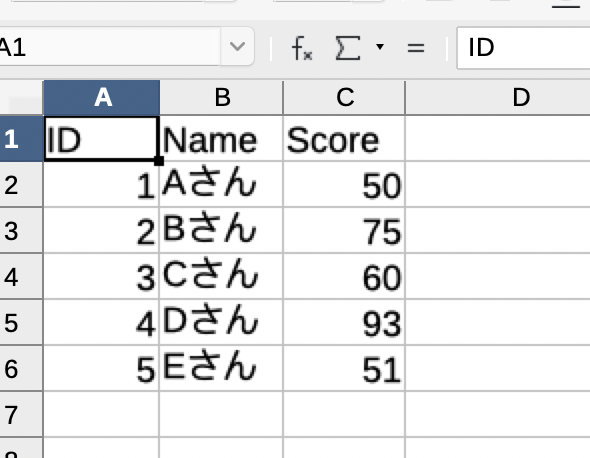
\includegraphics[width=0.5\textwidth,height=\textheight]{./Figs/IO/Export.png}

}

\caption{\label{fig-io_export}my\_data.csvの中身}

\end{figure}

\hypertarget{rdataux30d5ux30a1ux30a4ux30eb}{%
\subsection{RDataファイル}\label{rdataux30d5ux30a1ux30a4ux30eb}}

最後に\texttt{.RData}形式でデータを書き出してみよう。今回は先ほど作成した\texttt{my\_data}と、以下で作成する\texttt{numeric\_vec1}、\texttt{numeric\_vec2}、\texttt{character\_vec}を\texttt{my\_RData.RData}という名のファイルとして
\texttt{Data}フォルダに書き出す。使用する関数は \texttt{save()}
である。引数として保存するオブジェクト名をすべてカンマ区切りで書き、最後に\texttt{file} 引数でファイル名を指定すればよい。

\begin{Shaded}
\begin{Highlighting}[numbers=left,,]
\NormalTok{numeric\_vec1  }\OtherTok{\textless{}{-}} \FunctionTok{c}\NormalTok{(}\DecValTok{1}\NormalTok{, }\DecValTok{5}\NormalTok{, }\DecValTok{3}\NormalTok{, }\DecValTok{6}\NormalTok{, }\DecValTok{99}\NormalTok{, }\DecValTok{2}\NormalTok{, }\DecValTok{8}\NormalTok{)}
\NormalTok{numeric\_vec2  }\OtherTok{\textless{}{-}} \DecValTok{1}\SpecialCharTok{:}\DecValTok{20}
\NormalTok{character\_vec }\OtherTok{\textless{}{-}} \FunctionTok{c}\NormalTok{(}\StringTok{\textquotesingle{}cat\textquotesingle{}}\NormalTok{, }\StringTok{\textquotesingle{}cheetah\textquotesingle{}}\NormalTok{, }\StringTok{\textquotesingle{}lion\textquotesingle{}}\NormalTok{, }\StringTok{\textquotesingle{}tiger\textquotesingle{}}\NormalTok{)}
\FunctionTok{save}\NormalTok{(my\_data, numeric\_vec1, numeric\_vec2, character\_vec, }
     \AttributeTok{file =} \StringTok{"Data/my\_RData.RData"}\NormalTok{)}
\end{Highlighting}
\end{Shaded}

 実際に\texttt{my\_RData.Rdata}ファイルが生成されているかを確認してみよう。ファイルの保存がうまくいっていれば、\texttt{my\_RData.Rdata}を読み込むだけで、\texttt{my\_data}、\texttt{numeric\_vec1}、\texttt{numeric\_vec2}、\texttt{character\_vec}
という4つのオブジェクトを一挙に作業スペースに読み込むことができるはずだ。実際にできるか確認しよう。そのために、まず現在の実行環境上にある\texttt{my\_ata}、\texttt{numeric\_vec1}、\texttt{numeric\_vec2}、\texttt{character\_vec}を削除する。そのために
\texttt{rm()} 関数を使う。

\begin{Shaded}
\begin{Highlighting}[numbers=left,,]
\FunctionTok{rm}\NormalTok{(my\_data)}
\FunctionTok{rm}\NormalTok{(numeric\_vec1)}
\FunctionTok{rm}\NormalTok{(numeric\_vec2)}
\FunctionTok{rm}\NormalTok{(character\_vec)}
\end{Highlighting}
\end{Shaded}

 このコードは以下のように1行のコードに書き換えられる。

\begin{Shaded}
\begin{Highlighting}[numbers=left,,]
\FunctionTok{rm}\NormalTok{(}\AttributeTok{list =} \FunctionTok{c}\NormalTok{(}\StringTok{"my\_data"}\NormalTok{, }\StringTok{"numeric\_vec1"}\NormalTok{, }\StringTok{"numeric\_vec2"}\NormalTok{, }\StringTok{"character\_vec"}\NormalTok{))}
\end{Highlighting}
\end{Shaded}

 4のオブジェクトが削除されたか、\texttt{ls()}関数で確認しよう。

\begin{Shaded}
\begin{Highlighting}[numbers=left,,]
\FunctionTok{ls}\NormalTok{()}
\end{Highlighting}
\end{Shaded}

\begin{verbatim}
[1] "EnglishScore" "Excel_DF"     "MathScore"    "my_df1"       "ShiftJIS_df1"
[6] "ShiftJIS_df2" "ShiftJIS_df3" "Stata_DF"     "UTF8_df"     
\end{verbatim}

それでは\texttt{Data}フォルダー内の\texttt{my\_RData.RData}を読み込み、4つのオブジェクトが実行環境に読み込まれるか確認しよう。

\begin{Shaded}
\begin{Highlighting}[numbers=left,,]
\FunctionTok{load}\NormalTok{(}\StringTok{"Data/my\_RData.RData"}\NormalTok{) }\CommentTok{\# Dataフォルダー内のmy\_RData.RDataを読み込む}
\FunctionTok{ls}\NormalTok{()                        }\CommentTok{\# 作業スペース上のオブジェクトのリストを確認する}
\end{Highlighting}
\end{Shaded}

\begin{verbatim}
 [1] "character_vec" "EnglishScore"  "Excel_DF"      "MathScore"    
 [5] "my_data"       "my_df1"        "numeric_vec1"  "numeric_vec2" 
 [9] "ShiftJIS_df1"  "ShiftJIS_df2"  "ShiftJIS_df3"  "Stata_DF"     
[13] "UTF8_df"      
\end{verbatim}

\hypertarget{sec-datatype}{%
\chapter{データ型}\label{sec-datatype}}

\begin{Shaded}
\begin{Highlighting}[numbers=left,,]
\NormalTok{pacman}\SpecialCharTok{::}\FunctionTok{p\_load}\NormalTok{(tidyverse)}
\end{Highlighting}
\end{Shaded}

\hypertarget{sec-type_intro}{%
\section{データ型とは}\label{sec-type_intro}}

ここではRにおけるデータ型について説明します。第\ref{sec-datastructure}章で説明するデータ「構造」とデータ「型」は異なる概念です。次章でも説明しますが、Rにおけるデータの最小単位はベクトルです。\texttt{c(1,\ 2,\ 3,\ 4,\ 5)}や\texttt{c("Yanai",\ "Song",\ "Hadley")}もベクトルですが、\texttt{30}とか\texttt{"R"}もベクトルです。後者のように要素が1つのベクトルは原子ベクトル
(atomic
vector)とも呼ばれますが、本質的には普通ベクトルです。このベクトルの要素の性質がデータ型です。たとえば\texttt{c(2,\ 3,\ 5,\ 7,\ 11)}は数値型ですし、\texttt{c("R",\ "Python",\ "Julia")}は文字型です。他にも第\ref{sec-rbasic}章で紹介した\texttt{FALSE}や\texttt{TRUE}は論理型と呼ばれています。一つのベクトルは複数の要素で構成されることも可能ですが、必ず\textbf{同じデータ型}である必要があります。

しかし、データ分析を行う際はベクトル以外のデータも多いです。行列や表がその典型例です。しかし、行列でも表でも中身の一つ一つの要素は長さ1のベクトルに過ぎません。たとえば、以下のような2行5列のベクトルがあるとします。ここで1行3列目の要素は\texttt{11}であり、長さ1の数値型ベクトルです。あるいは5列目は\texttt{c(23,\ 29)}であり、長さ2の数値型ベクトルです。

\begin{verbatim}
     [,1] [,2] [,3] [,4] [,5]
[1,]    2    5   11   17   23
[2,]    3    7   13   19   29
\end{verbatim}

表についても考えてみましょう。以下の表の3行2列目の要素は\texttt{"American\ Samoa"}という長さ1の文字型ベクトルです。また、6列目は\texttt{c("UEFA",\ "CAF",\ "OFC",\ "UEFA",\ "CAF",\ "CONCACAF")}であり、これは長さ6の文字型ベクトルです。このようにRで扱う全てのデータは複数のベクトルが集まっているものです。

\begin{verbatim}
  ID                Team Rank Points Prev_Points Confederation
1  1             Albania   75   1325        1316          UEFA
2  2             Algeria   85   1271        1271           CAF
3  3      American Samoa  133   1030        1030           OFC
4  4             Andorra  155    749         749          UEFA
5  5              Angola  121   1117        1117           CAF
6  6 Antigua and Barbuda  153    787         787      CONCACAF
\end{verbatim}

つまり、複数のベクトルを綺麗に、または分析しやすく集めたのが行列や表であり、これがデータ構造に該当します。データ型ごとの処理方法については本書を通じて紹介して行きますので、本章は軽く読んで頂いても構いません。ただし、Factor型とDate
\&
Datetime型の処理はやや特殊ですので、手を動かしながら読み進めることをおすすめします。

ここではデータ型について紹介し、次章ではデータ構造について解説します。

\begin{center}\rule{0.5\linewidth}{0.5pt}\end{center}

\hypertarget{sec-type_logical}{%
\section{Logical}\label{sec-type_logical}}

Logical型は\texttt{TRUE}と\texttt{FALSE}のみで構成されたデータ型です。練習としてなにかの長さ5の論理型ベクトルを作ってみましょう。

\begin{Shaded}
\begin{Highlighting}[numbers=left,,]
\NormalTok{Logical.Vec1 }\OtherTok{\textless{}{-}} \FunctionTok{c}\NormalTok{(}\ConstantTok{TRUE}\NormalTok{, }\ConstantTok{FALSE}\NormalTok{, }\ConstantTok{TRUE}\NormalTok{, }\ConstantTok{TRUE}\NormalTok{, }\ConstantTok{FALSE}\NormalTok{)}

\NormalTok{Logical.Vec1}
\end{Highlighting}
\end{Shaded}

\begin{verbatim}
[1]  TRUE FALSE  TRUE  TRUE FALSE
\end{verbatim}

注意すべきこととしては、\texttt{TRUE}と\texttt{FALSE}は\texttt{"}で囲まないことです。\texttt{"TRUE"}、\texttt{"FALSE"}と入力してしまえばlogical
型として認識されません。もし、一つ間違えて2番目の要素である\texttt{FALSE}を\texttt{"FALSE"}と入力したらどうなるでしょうか。

\begin{Shaded}
\begin{Highlighting}[numbers=left,,]
\NormalTok{Logical.Vec2 }\OtherTok{\textless{}{-}} \FunctionTok{c}\NormalTok{(}\ConstantTok{TRUE}\NormalTok{, }\StringTok{"FALSE"}\NormalTok{, }\ConstantTok{TRUE}\NormalTok{, }\ConstantTok{TRUE}\NormalTok{, }\ConstantTok{FALSE}\NormalTok{)}

\NormalTok{Logical.Vec2}
\end{Highlighting}
\end{Shaded}

\begin{verbatim}
[1] "TRUE"  "FALSE" "TRUE"  "TRUE"  "FALSE"
\end{verbatim}

2番目の要素だけでなく、他の全ての要素も\texttt{"}で囲まれるようになりました。実際に、この2つのベクトルのデータ型を確認してみましょう。ベクトルのデータ型を確認する関数は\texttt{class()}関数です。

\begin{Shaded}
\begin{Highlighting}[numbers=left,,]
\FunctionTok{class}\NormalTok{(Logical.Vec1)}
\end{Highlighting}
\end{Shaded}

\begin{verbatim}
[1] "logical"
\end{verbatim}

\begin{Shaded}
\begin{Highlighting}[numbers=left,,]
\FunctionTok{class}\NormalTok{(Logical.Vec2)}
\end{Highlighting}
\end{Shaded}

\begin{verbatim}
[1] "character"
\end{verbatim}

\texttt{Logical.Vec1}はlogical型ですが、\texttt{Logical.Vec2}はcharacter型と認識されます。

他にも、\texttt{is.logical()}関数を使ってあるベクトルがlogical型か否かを判定することも可能です。もし、ベクトルがlogical型なら\texttt{TRUE}が、logical型以外なら\texttt{FALSE}が返って来ます。

\begin{Shaded}
\begin{Highlighting}[numbers=left,,]
\FunctionTok{is.logical}\NormalTok{(Logical.Vec1)}
\end{Highlighting}
\end{Shaded}

\begin{verbatim}
[1] TRUE
\end{verbatim}

\begin{Shaded}
\begin{Highlighting}[numbers=left,,]
\FunctionTok{is.logical}\NormalTok{(Logical.Vec2)}
\end{Highlighting}
\end{Shaded}

\begin{verbatim}
[1] FALSE
\end{verbatim}

Logical型は様々な場面で使われますが、代表的な使い方は第\ref{sec-rbasic_calc}章で紹介しました要素の抽出と第\ref{sec-programming}章で紹介する予定の条件分岐
(\texttt{if()}や\texttt{ifelse()})、条件反復
(\texttt{while()})があります。

\begin{center}\rule{0.5\linewidth}{0.5pt}\end{center}

\hypertarget{sec-type_numeric}{%
\section{Numeric}\label{sec-type_numeric}}

Numeric型は数値型ですが、まずはnumeric型のベクトル\texttt{Numeric.Vec1}を作成し、データ型を確認してみましょう。

\begin{Shaded}
\begin{Highlighting}[numbers=left,,]
\NormalTok{Numeric.Vec1 }\OtherTok{\textless{}{-}} \FunctionTok{c}\NormalTok{(}\DecValTok{2}\NormalTok{, }\DecValTok{0}\NormalTok{, }\DecValTok{0}\NormalTok{, }\DecValTok{1}\NormalTok{, }\DecValTok{3}\NormalTok{)}

\FunctionTok{class}\NormalTok{(Numeric.Vec1)}
\end{Highlighting}
\end{Shaded}

\begin{verbatim}
[1] "numeric"
\end{verbatim}

\texttt{is.logical()}に似た関数\texttt{is.numeric()}も使用可能です。

\begin{Shaded}
\begin{Highlighting}[numbers=left,,]
\FunctionTok{is.numeric}\NormalTok{(Numeric.Vec1)}
\end{Highlighting}
\end{Shaded}

\begin{verbatim}
[1] TRUE
\end{verbatim}

\begin{Shaded}
\begin{Highlighting}[numbers=left,,]
\FunctionTok{is.numeric}\NormalTok{(Logical.Vec1)}
\end{Highlighting}
\end{Shaded}

\begin{verbatim}
[1] FALSE
\end{verbatim}

もうちょっと詳しく分けるとinteger型とdouble型があります。以下の内容はあまり意識的に区分して使う場面が稀ですので、(読み)飛ばしても構いません。

integerは整数型であり、doubleは実数型です。これは\texttt{class()}関数では確認できず、\texttt{typeof()}関すを使います。

\begin{Shaded}
\begin{Highlighting}[numbers=left,,]
\FunctionTok{typeof}\NormalTok{(Numeric.Vec1)}
\end{Highlighting}
\end{Shaded}

\begin{verbatim}
[1] "double"
\end{verbatim}

一般的に作成するnumeric型のベクトルは全てdouble型です。もし、整数型のベクトルを作成したい場合、数値の後ろに\texttt{L}を付けます。

\begin{Shaded}
\begin{Highlighting}[numbers=left,,]
\NormalTok{Integer.Vec1 }\OtherTok{\textless{}{-}} \FunctionTok{c}\NormalTok{(2L, 0L, 0L, 1L, 3L)}
\FunctionTok{typeof}\NormalTok{(Integer.Vec1)}
\end{Highlighting}
\end{Shaded}

\begin{verbatim}
[1] "integer"
\end{verbatim}

ここでも注意すべき点としては、一つでも\texttt{L}が付かない要素が含まれる場合、自動的にdouble型に変換されるという点です。

\begin{Shaded}
\begin{Highlighting}[numbers=left,,]
\NormalTok{Integer.Vec2 }\OtherTok{\textless{}{-}} \FunctionTok{c}\NormalTok{(2L, 0L, }\DecValTok{0}\NormalTok{, 1L, 3L)}
\FunctionTok{typeof}\NormalTok{(Integer.Vec2)}
\end{Highlighting}
\end{Shaded}

\begin{verbatim}
[1] "double"
\end{verbatim}

もちろんですが、小数点のある数値に\texttt{L}を付けてもinteger型にはならず、勝手にdouble型になります。また、integer型同士の割り算の結果もdouble型になります。これは\texttt{2L/1L}のような場合でも同じです。足し算、引き算、掛け算はinteger型になります。

\begin{Shaded}
\begin{Highlighting}[numbers=left,,]
\FunctionTok{typeof}\NormalTok{(}\FloatTok{2.3}\NormalTok{L)}
\end{Highlighting}
\end{Shaded}

\begin{verbatim}
[1] "double"
\end{verbatim}

\begin{Shaded}
\begin{Highlighting}[numbers=left,,]
\FunctionTok{typeof}\NormalTok{(3L }\SpecialCharTok{/}\NormalTok{ 12L)}
\end{Highlighting}
\end{Shaded}

\begin{verbatim}
[1] "double"
\end{verbatim}

\begin{Shaded}
\begin{Highlighting}[numbers=left,,]
\FunctionTok{typeof}\NormalTok{(3L }\SpecialCharTok{/}\NormalTok{ 1L)}
\end{Highlighting}
\end{Shaded}

\begin{verbatim}
[1] "double"
\end{verbatim}

\begin{Shaded}
\begin{Highlighting}[numbers=left,,]
\FunctionTok{typeof}\NormalTok{(3L }\SpecialCharTok{+}\NormalTok{ 1L)}
\end{Highlighting}
\end{Shaded}

\begin{verbatim}
[1] "integer"
\end{verbatim}

\begin{Shaded}
\begin{Highlighting}[numbers=left,,]
\FunctionTok{typeof}\NormalTok{(3L }\SpecialCharTok{{-}}\NormalTok{ 4L)}
\end{Highlighting}
\end{Shaded}

\begin{verbatim}
[1] "integer"
\end{verbatim}

\begin{Shaded}
\begin{Highlighting}[numbers=left,,]
\FunctionTok{typeof}\NormalTok{(3L }\SpecialCharTok{*}\NormalTok{ 6L)}
\end{Highlighting}
\end{Shaded}

\begin{verbatim}
[1] "integer"
\end{verbatim}

一般的な分析において整数と実数を厳格に区別して使う場面は多くないと考えられますので、今のところはあまり気にしなくても問題ないでしょう。

\begin{center}\rule{0.5\linewidth}{0.5pt}\end{center}

\hypertarget{sec-type_complex}{%
\section{Complex}\label{sec-type_complex}}

Complex型は複素数を表すデータ型であり、\texttt{実数部+虚数部i}のように表記します。まず、複素数のベクトル\texttt{Complex.Vec1}を作成し、データ型を確認してみましょう。

\begin{Shaded}
\begin{Highlighting}[numbers=left,,]
\NormalTok{Complex.Vec1 }\OtherTok{\textless{}{-}} \FunctionTok{c}\NormalTok{(}\DecValTok{1}\SpecialCharTok{+}\NormalTok{3i, }\DecValTok{3}\SpecialCharTok{+}\NormalTok{2i, }\FloatTok{2.5}\SpecialCharTok{+}\NormalTok{7i)}
\NormalTok{Complex.Vec1}
\end{Highlighting}
\end{Shaded}

\begin{verbatim}
[1] 1.0+3i 3.0+2i 2.5+7i
\end{verbatim}

\begin{Shaded}
\begin{Highlighting}[numbers=left,,]
\FunctionTok{class}\NormalTok{(Complex.Vec1)}
\end{Highlighting}
\end{Shaded}

\begin{verbatim}
[1] "complex"
\end{verbatim}

あまりおすすめはできませんが、\texttt{虚数部i+実数部}のような書き方も可能です。

\begin{Shaded}
\begin{Highlighting}[numbers=left,,]
\NormalTok{Complex.Vec2 }\OtherTok{\textless{}{-}} \FunctionTok{c}\NormalTok{(3i}\SpecialCharTok{+}\DecValTok{1}\NormalTok{, 2i}\SpecialCharTok{+}\DecValTok{3}\NormalTok{, 7i}\FloatTok{+2.5}\NormalTok{)}
\NormalTok{Complex.Vec2}
\end{Highlighting}
\end{Shaded}

\begin{verbatim}
[1] 1.0+3i 3.0+2i 2.5+7i
\end{verbatim}

\begin{Shaded}
\begin{Highlighting}[numbers=left,,]
\FunctionTok{class}\NormalTok{(Complex.Vec2)}
\end{Highlighting}
\end{Shaded}

\begin{verbatim}
[1] "complex"
\end{verbatim}

\texttt{Complex.Vec1}と\texttt{Complex.Vec2}は同じベクトルであることを確認してみましょう。

\begin{Shaded}
\begin{Highlighting}[numbers=left,,]
\NormalTok{Complex.Vec1 }\SpecialCharTok{==}\NormalTok{ Complex.Vec2}
\end{Highlighting}
\end{Shaded}

\begin{verbatim}
[1] TRUE TRUE TRUE
\end{verbatim}

もし、ベクトル内にnumeric型とcomplex型が混在している場合、強制的にcomplex型に変換されます。変換された後の値は\texttt{実数部+0i}のようになります。

\begin{Shaded}
\begin{Highlighting}[numbers=left,,]
\NormalTok{Complex.Vec3 }\OtherTok{\textless{}{-}} \FunctionTok{c}\NormalTok{(}\DecValTok{2}\SpecialCharTok{+}\NormalTok{7i, }\DecValTok{5}\NormalTok{, }\DecValTok{13}\SpecialCharTok{+}\NormalTok{1i)}
\NormalTok{Complex.Vec3}
\end{Highlighting}
\end{Shaded}

\begin{verbatim}
[1]  2+7i  5+0i 13+1i
\end{verbatim}

\begin{Shaded}
\begin{Highlighting}[numbers=left,,]
\FunctionTok{class}\NormalTok{(Complex.Vec3)}
\end{Highlighting}
\end{Shaded}

\begin{verbatim}
[1] "complex"
\end{verbatim}

\begin{center}\rule{0.5\linewidth}{0.5pt}\end{center}

\hypertarget{sec-type_character}{%
\section{Character}\label{sec-type_character}}

Character型は文字列で構成されているデータ型です。Rを含む多くの言語は文字列を表現するために、中身を\texttt{"}で囲みます。\texttt{"abc"}はcharacter型ですが、\texttt{"1"}や\texttt{"3+5i"}もcharacter型です。数字であっても\texttt{"}で囲んだらそれは文字列となります。それではいくつかのcharacter型ベクトルを作っていみましょう。

\begin{Shaded}
\begin{Highlighting}[numbers=left,,]
\NormalTok{Char.Vec1 }\OtherTok{\textless{}{-}} \FunctionTok{c}\NormalTok{(}\StringTok{"Yanai"}\NormalTok{, }\StringTok{"Song"}\NormalTok{, }\StringTok{"Shigemura"}\NormalTok{, }\StringTok{"Tani"}\NormalTok{)}
\NormalTok{Char.Vec2 }\OtherTok{\textless{}{-}} \FunctionTok{c}\NormalTok{(}\DecValTok{1}\NormalTok{, }\DecValTok{2}\NormalTok{, }\DecValTok{3}\NormalTok{, }\DecValTok{4}\NormalTok{)}
\NormalTok{Char.Vec3 }\OtherTok{\textless{}{-}} \FunctionTok{c}\NormalTok{(}\StringTok{"1"}\NormalTok{, }\StringTok{"2"}\NormalTok{, }\StringTok{"3"}\NormalTok{, }\StringTok{"4"}\NormalTok{)}

\NormalTok{Char.Vec1}
\end{Highlighting}
\end{Shaded}

\begin{verbatim}
[1] "Yanai"     "Song"      "Shigemura" "Tani"     
\end{verbatim}

\begin{Shaded}
\begin{Highlighting}[numbers=left,,]
\NormalTok{Char.Vec2}
\end{Highlighting}
\end{Shaded}

\begin{verbatim}
[1] 1 2 3 4
\end{verbatim}

\begin{Shaded}
\begin{Highlighting}[numbers=left,,]
\NormalTok{Char.Vec3}
\end{Highlighting}
\end{Shaded}

\begin{verbatim}
[1] "1" "2" "3" "4"
\end{verbatim}

\texttt{Char.Vec2}と\texttt{Char.Vec3}の違いは通じを\texttt{"}で囲んだか否かです。ベクトルの中身を見ても、\texttt{Char.Vec2}は\texttt{"}で囲まれていません。データ型を見てみましょう。

\begin{Shaded}
\begin{Highlighting}[numbers=left,,]
\FunctionTok{class}\NormalTok{(Char.Vec1)}
\end{Highlighting}
\end{Shaded}

\begin{verbatim}
[1] "character"
\end{verbatim}

\begin{Shaded}
\begin{Highlighting}[numbers=left,,]
\FunctionTok{class}\NormalTok{(Char.Vec2)}
\end{Highlighting}
\end{Shaded}

\begin{verbatim}
[1] "numeric"
\end{verbatim}

\begin{Shaded}
\begin{Highlighting}[numbers=left,,]
\FunctionTok{class}\NormalTok{(Char.Vec3)}
\end{Highlighting}
\end{Shaded}

\begin{verbatim}
[1] "character"
\end{verbatim}

やはり\texttt{Char.Vec3}もcharacter型になっていることが分かります。

\begin{center}\rule{0.5\linewidth}{0.5pt}\end{center}

\hypertarget{sec-type_factor}{%
\section{Factor}\label{sec-type_factor}}

Factor型はラベル付きの数値型データです。Factor型の詳細な扱い方については第\ref{sec-factor}章で詳細に説明しますが、ここではfactor型がどういうデータ型なのかについてのみ紹介します。Factor型の見た目はcharacter型とほぼ同じですし、分析の場面においてもcharacter型とほぼ同じ扱いになります。Factor型とcharacter型との違いは、「順序が付いている」点です。例えば、以下の質問文に対するアンケートの結果を考えてみましょう。

\begin{itemize}
\tightlist
\item
  あなたは猫がすきですか。

  \begin{enumerate}
  \def\labelenumi{\arabic{enumi}.}
  \tightlist
  \item
    めちゃめちゃ好き
  \item
    めちゃ好き
  \item
    好き
  \item
    どちらかといえば好き
  \end{enumerate}
\end{itemize}

以下の 表~\ref{tbl-cat} は5人の結果です。

\hypertarget{tbl-cat}{}
\begin{table}
\caption{\label{tbl-cat}猫をこよなく愛する5人 }

\centering
\begin{tabular}{r|l|l}
\hline
ID & Name & Cat\\
\hline
1 & Yanai & めちゃめちゃ好き\\
\hline
2 & Song & めちゃめちゃ好き\\
\hline
3 & Shigemura & どちらかといえば好き\\
\hline
4 & Tani & めちゃ好き\\
\hline
5 & Hadley & 好き\\
\hline
\end{tabular}
\end{table}

人間としてはこの表から、\href{https://soheishigemura.com}{重村}という人がどれだけ猫が嫌いなのかが分かります。ただし、Rはそうではありません。Rは日本語どころか、人間の言葉は理解できません。各項目ごとに順番を付けてあげる必要がありますが、そのために使われるのがfactor型です。

実習のために 表~\ref{tbl-cat}
の\texttt{Cat}列のみのベクトルを作ってみましょう。

\begin{Shaded}
\begin{Highlighting}[numbers=left,,]
\NormalTok{Factor.Vec1 }\OtherTok{\textless{}{-}} \FunctionTok{c}\NormalTok{(}\StringTok{"めちゃめちゃ好き"}\NormalTok{, }\StringTok{"めちゃめちゃ好き"}\NormalTok{, }
                 \StringTok{"どちらかといえば好き"}\NormalTok{, }\StringTok{"めちゃ好き"}\NormalTok{, }\StringTok{"好き"}\NormalTok{)}

\NormalTok{Factor.Vec1}
\end{Highlighting}
\end{Shaded}

\begin{verbatim}
[1] "めちゃめちゃ好き"     "めちゃめちゃ好き"     "どちらかといえば好き"
[4] "めちゃ好き"           "好き"                
\end{verbatim}

\begin{Shaded}
\begin{Highlighting}[numbers=left,,]
\FunctionTok{class}\NormalTok{(Factor.Vec1)}
\end{Highlighting}
\end{Shaded}

\begin{verbatim}
[1] "character"
\end{verbatim}

\texttt{Factor.Vec1}は普通の文字列ベクトルであることが分かります。これをfactor型に変換するためには\texttt{factor()}関数を使います。

\begin{Shaded}
\begin{Highlighting}[numbers=left,,]
\NormalTok{Factor.Vec2 }\OtherTok{\textless{}{-}} \FunctionTok{factor}\NormalTok{(Factor.Vec1, }\AttributeTok{ordered =} \ConstantTok{TRUE}\NormalTok{,}
                      \AttributeTok{levels =} \FunctionTok{c}\NormalTok{(}\StringTok{"どちらかといえば好き"}\NormalTok{, }\StringTok{"好き"}\NormalTok{,}
                                 \StringTok{"めちゃ好き"}\NormalTok{, }\StringTok{"めちゃめちゃ好き"}\NormalTok{))}
\FunctionTok{class}\NormalTok{(Factor.Vec2)}
\end{Highlighting}
\end{Shaded}

\begin{verbatim}
[1] "ordered" "factor" 
\end{verbatim}

データ型がfactor型に変換されています。\texttt{"ordered"}というものも付いていますが、これについては後ほど説明します。それでは中身をみましょう。

\begin{Shaded}
\begin{Highlighting}[numbers=left,,]
\NormalTok{Factor.Vec2}
\end{Highlighting}
\end{Shaded}

\begin{verbatim}
[1] めちゃめちゃ好き     めちゃめちゃ好き     どちらかといえば好き
[4] めちゃ好き           好き                
Levels: どちらかといえば好き < 好き < めちゃ好き < めちゃめちゃ好き
\end{verbatim}

いくつかの点で異なります。まず、文字列であるにもかかわらず、\texttt{"}で囲まれていいない点です。そして3行目に\texttt{4\ Levels:}というのが追加されている点です。このlevelは「水準」と呼ばれるものです。\texttt{4\ Levels}ですから、\texttt{Factor.Vec2}は4つの水準で構成されていることを意味します。Factor型の値は予め指定された水準以外の値を取ることはできません。たとえば、2番目の要素を「超好き」に変えてみましょう。

\begin{Shaded}
\begin{Highlighting}[numbers=left,,]
\NormalTok{Factor.Vec2[}\DecValTok{2}\NormalTok{] }\OtherTok{\textless{}{-}} \StringTok{"超好き"}
\end{Highlighting}
\end{Shaded}

\begin{verbatim}
Warning in `[<-.factor`(`*tmp*`, 2, value = "超好き"): invalid factor level, NA
generated
\end{verbatim}

\begin{Shaded}
\begin{Highlighting}[numbers=left,,]
\NormalTok{Factor.Vec2}
\end{Highlighting}
\end{Shaded}

\begin{verbatim}
[1] めちゃめちゃ好き     <NA>                 どちらかといえば好き
[4] めちゃ好き           好き                
Levels: どちらかといえば好き < 好き < めちゃ好き < めちゃめちゃ好き
\end{verbatim}

警告が表示され、2番目の要素が後ほど紹介する欠損値となっていることが分かります。それでは普通に「好き」を入れてみましょう。

\begin{Shaded}
\begin{Highlighting}[numbers=left,,]
\NormalTok{Factor.Vec2[}\DecValTok{2}\NormalTok{] }\OtherTok{\textless{}{-}} \StringTok{"好き"}
\NormalTok{Factor.Vec2}
\end{Highlighting}
\end{Shaded}

\begin{verbatim}
[1] めちゃめちゃ好き     好き                 どちらかといえば好き
[4] めちゃ好き           好き                
Levels: どちらかといえば好き < 好き < めちゃ好き < めちゃめちゃ好き
\end{verbatim}

今回は問題なく置換できましたね。このようにfactor型の取りうる値は既に指定されています。また、\texttt{\#\#\ 4\ Levels:\ どちらかといえば好き\ \textless{}\ 好き\ \textless{}\ ...\ \textless{}\ めちゃめちゃ好き}からも分かるように、その大小関係の情報も含まれています。猫好きの度合いは「どちらかといえば好き-好き-めちゃ好き-めちゃめちゃ好き」の順で高くなることをRも認識できるようになりました。

Factor型はこのように順序付きデータを扱う際に便利なデータ型ですが、順序情報を含まないfactor型もあります。これは\texttt{factor()}を使う際、\texttt{ordered\ =\ TRUE}引数を削除するだけでできます。

\begin{Shaded}
\begin{Highlighting}[numbers=left,,]
\NormalTok{Factor.Vec3 }\OtherTok{\textless{}{-}} \FunctionTok{factor}\NormalTok{(Factor.Vec1,}
                      \AttributeTok{levels =} \FunctionTok{c}\NormalTok{(}\StringTok{"どちらかといえば好き"}\NormalTok{, }\StringTok{"好き"}\NormalTok{,}
                                 \StringTok{"めちゃ好き"}\NormalTok{, }\StringTok{"めちゃめちゃ好き"}\NormalTok{))}
\NormalTok{Factor.Vec3}
\end{Highlighting}
\end{Shaded}

\begin{verbatim}
[1] めちゃめちゃ好き     めちゃめちゃ好き     どちらかといえば好き
[4] めちゃ好き           好き                
Levels: どちらかといえば好き 好き めちゃ好き めちゃめちゃ好き
\end{verbatim}

\begin{Shaded}
\begin{Highlighting}[numbers=left,,]
\FunctionTok{class}\NormalTok{(Factor.Vec3)}
\end{Highlighting}
\end{Shaded}

\begin{verbatim}
[1] "factor"
\end{verbatim}

今回は3行目が\texttt{\#\#\ Levels:\ どちらかといえば好き\ 好き\ めちゃ好き\ めちゃめちゃ好き}となり、順序に関する情報がなくなりました。また、\texttt{class()}で確認しましたデータ型に\texttt{"ordered"}が付いていません。これは順序なしfactor型であることを意味します。「順序付けしないならfactor型は要らないのでは\ldots?」と思うかも知れませんが、これはこれで便利です。その例を考えてみましょう。

分析においてfactor型はcharacter型に近い役割を果たしますが、factor型なりの長所もあります。それは図や表を作成する際です。例えば、横軸が都道府県名で、縦軸がその都道府県の財政力指数を表す棒グラフを作成するとします。元になるデータは
表~\ref{tbl-zaisei} の\texttt{Zaisei\_df}です。

\hypertarget{tbl-zaisei}{}
\begin{table}
\caption{\label{tbl-zaisei}5都道府県のH29財政力指数 }

\centering
\begin{tabular}{r|l|r}
\hline
ID & Pref & Zaisei\\
\hline
1 & Hokkaido & 0.44396\\
\hline
2 & Tokyo & 1.19157\\
\hline
3 & Aichi & 0.92840\\
\hline
4 & Osaka & 0.78683\\
\hline
5 & Fukuoka & 0.64322\\
\hline
\end{tabular}
\end{table}

可視化については第\ref{sec-visualization1}章以降で詳しく解説しますが、この\texttt{Pref}列をcharacter型にしたままグラフにしますと
図~\ref{fig-zaisei_fig} のようになります。

\begin{figure}

{\centering 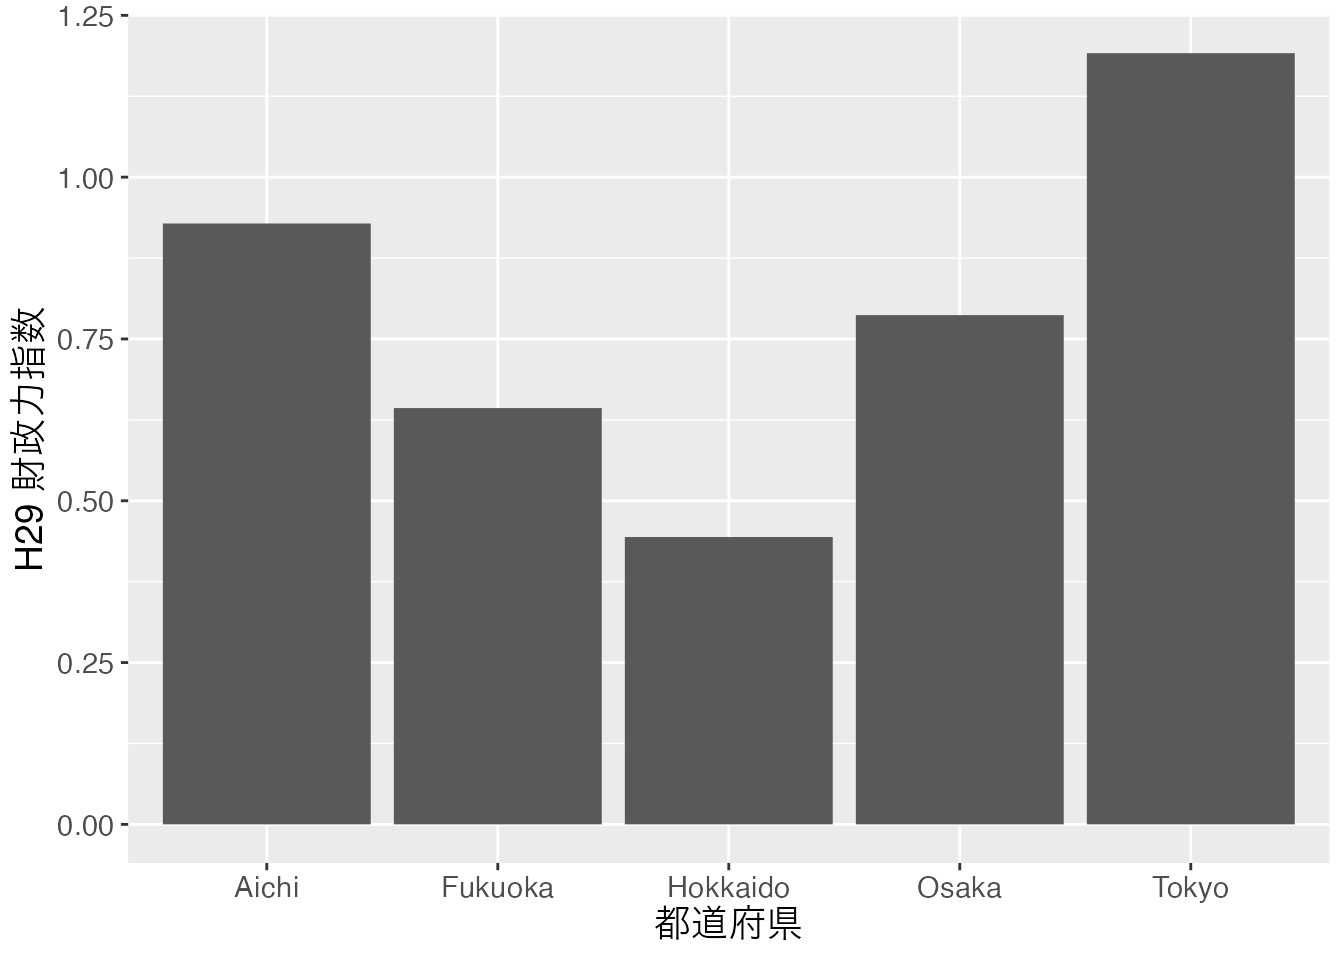
\includegraphics{./datatype_files/figure-pdf/fig-zaisei_fig-1.png}

}

\caption{\label{fig-zaisei_fig}5都道府県のH29財政力指数}

\end{figure}

このようにアルファベット順で横軸が並び替えられます。別にこれでも問題ないと思う方もいるかも知れませんが、基本的に日本の都道府県は北から南の方へ並べるのが一般的な作法です\footnote{アメリカの州ならアルファベット順ですね。}。北海道と東京、大阪の間には順序関係はありません。しかし、表示される順番は固定したい。この場合、順序なしfactor型が活躍します。これを修正するためには\texttt{Pref}列を順序なしfactor型にすれば良いです\footnote{むろん、「北から南へ」という規則もあるので、順序付きfactor型にしても問題ありません。ただし、今回はあくまでも表示順番を設定したいだけですので、\texttt{ordered\ =\ TRUE}は省略しました。}。データフレームの列を修正する方法は第\ref{sec-datastructure}章で詳しく説明します。

\begin{Shaded}
\begin{Highlighting}[numbers=left,,]
\NormalTok{Zaisei\_df}\SpecialCharTok{$}\NormalTok{Pref }\OtherTok{\textless{}{-}} \FunctionTok{factor}\NormalTok{(Zaisei\_df}\SpecialCharTok{$}\NormalTok{Pref,}
                         \AttributeTok{levels =} \FunctionTok{c}\NormalTok{(}\StringTok{"Hokkaido"}\NormalTok{, }\StringTok{"Tokyo"}\NormalTok{, }\StringTok{"Aichi"}\NormalTok{, }\StringTok{"Osaka"}\NormalTok{, }\StringTok{"Fukuoka"}\NormalTok{))}
\end{Highlighting}
\end{Shaded}

\texttt{Zaisei.df}の\texttt{Pref}列を順序付きfactor型にしてから同じ図を描くと
図~\ref{fig-zaisei_fig2} のようになります。

\begin{figure}

{\centering 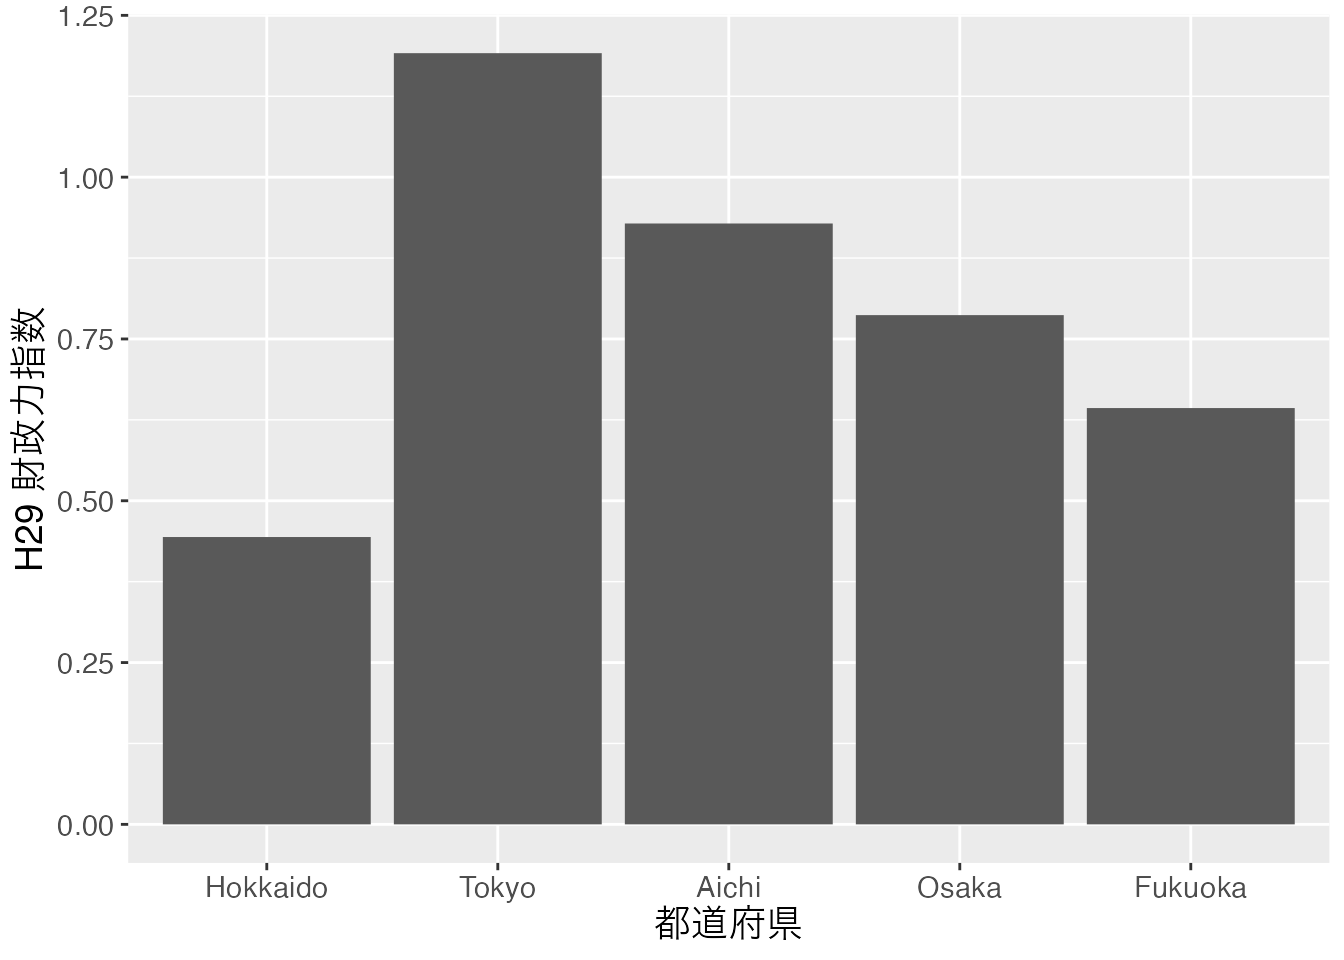
\includegraphics{./datatype_files/figure-pdf/fig-zaisei_fig2-1.png}

}

\caption{\label{fig-zaisei_fig2}5都道府県のH29財政力指数 (factor化済み)}

\end{figure}

都道府県以外にもこのような例は多くあります。順序尺度で測定された変数が代表的な例です。他にも政党名を議席数順で表示させたい場合もfactor型は有効でしょう。

\begin{center}\rule{0.5\linewidth}{0.5pt}\end{center}

\hypertarget{sec-type_date}{%
\section{Date}\label{sec-type_date}}

\hypertarget{ux306aux305cdateux578bux304cux3042ux308bux306eux304b}{%
\subsection{なぜDate型があるのか}\label{ux306aux305cdateux578bux304cux3042ux308bux306eux304b}}

Date型は年月日を表すデータ型\footnote{他にも時間まで表すDateTime型があります。}です。この2つのデータ型はかなり複雑ですが、ここでは簡単に説明します。Date型は日付の情報を含むため、順序関係が成立します。その意味では順序付きFactor型とあまり挙動は変わらないかもしれませんが、実際はそうではありません。

たとえば、Songの1週間\footnote{実際は2017年6月17日から11月15日まで記録しましたが、ここでは1週間分のみお見せします。}の睡眠時間を記録したデータ\texttt{SongSleep}があるとします。\texttt{Date}という列には日付が、\texttt{Sleep}列には睡眠時間が記録されています。睡眠時間の単位は「分」です。

\begin{Shaded}
\begin{Highlighting}[numbers=left,,]
\NormalTok{SongSleep }\OtherTok{\textless{}{-}} \FunctionTok{data.frame}\NormalTok{(}
    \AttributeTok{Date  =} \FunctionTok{c}\NormalTok{(}\StringTok{"2017{-}06{-}17"}\NormalTok{, }\StringTok{"2017{-}06{-}18"}\NormalTok{, }\StringTok{"2017{-}06{-}19"}\NormalTok{, }\StringTok{"2017{-}06{-}20"}\NormalTok{, }
              \StringTok{"2017{-}06{-}21"}\NormalTok{, }\StringTok{"2017{-}06{-}22"}\NormalTok{, }\StringTok{"2017{-}06{-}23"}\NormalTok{),}
    \AttributeTok{Sleep =} \FunctionTok{c}\NormalTok{(}\DecValTok{173}\NormalTok{, }\DecValTok{192}\NormalTok{, }\DecValTok{314}\NormalTok{, }\DecValTok{259}\NormalTok{, }\DecValTok{210}\NormalTok{, }\DecValTok{214}\NormalTok{, }\DecValTok{290}\NormalTok{)   }
\NormalTok{)}
\end{Highlighting}
\end{Shaded}

中身をみると、以下のようになります。

\begin{Shaded}
\begin{Highlighting}[numbers=left,,]
\NormalTok{SongSleep}
\end{Highlighting}
\end{Shaded}

\begin{verbatim}
        Date Sleep
1 2017-06-17   173
2 2017-06-18   192
3 2017-06-19   314
4 2017-06-20   259
5 2017-06-21   210
6 2017-06-22   214
7 2017-06-23   290
\end{verbatim}

日付を横軸に、睡眠時間を縦軸にした散布図を描くと 図~\ref{fig-sleep1}
このようになります。\{ggplot2\}を利用した作図については第\ref{sec-visualization1}章以降で解説しますので、ここではDate型の特徴のみ理解してもらえたら十分です。

\begin{figure}

{\centering 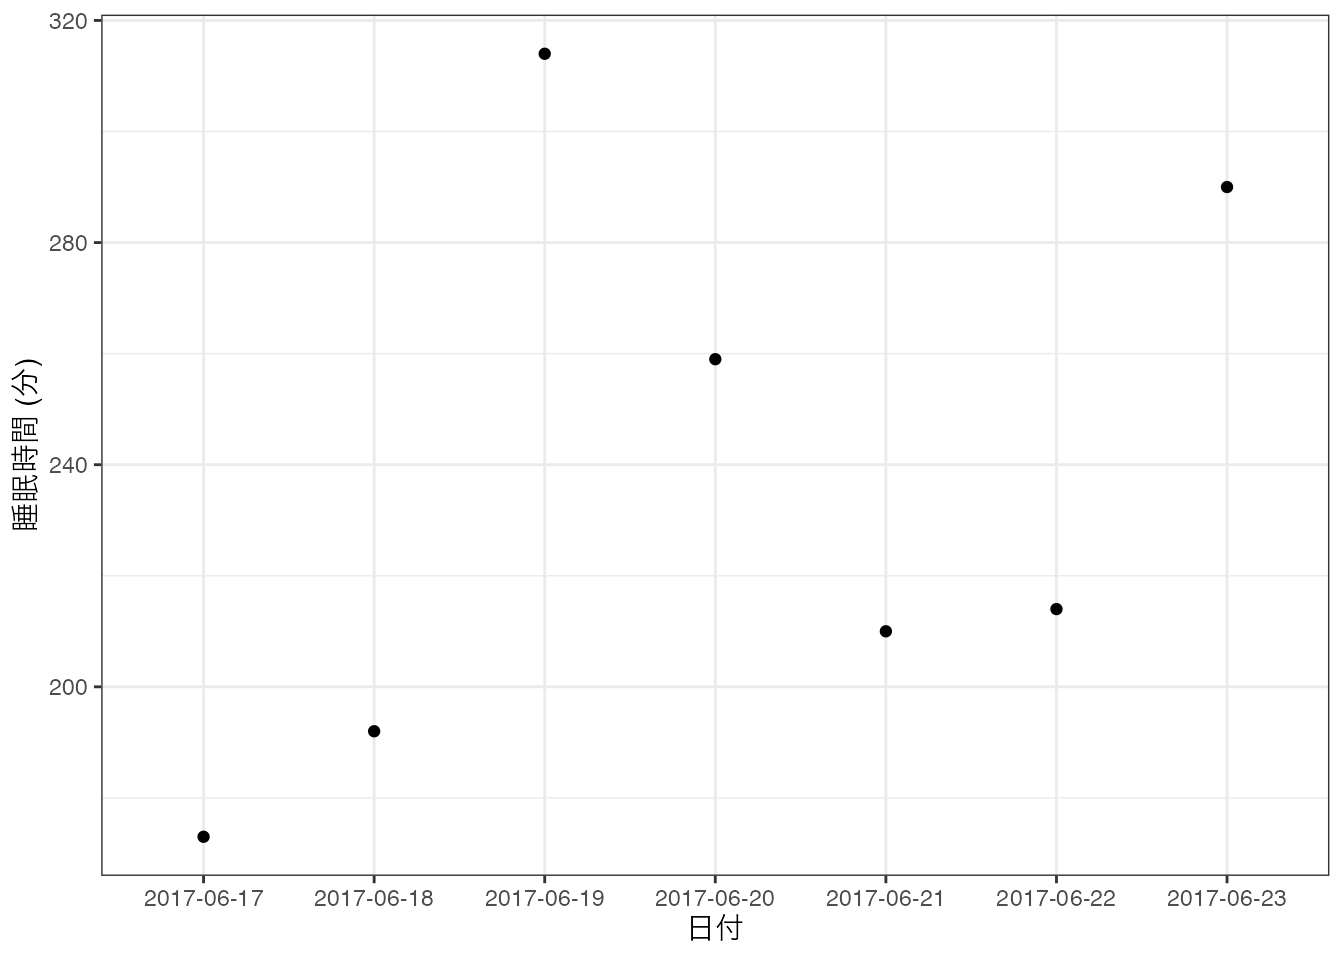
\includegraphics{./datatype_files/figure-pdf/fig-sleep1-1.png}

}

\caption{\label{fig-sleep1}Songの睡眠時間}

\end{figure}

この図は全く問題ないように見えます。それでは、\texttt{Date}列をそれぞれDate型に変換し、\texttt{SoongSleep}データの\texttt{DateD}としてみます。データフレームの列追加については第\ref{sec-datastructure_dataframe}章で解説します。

\begin{Shaded}
\begin{Highlighting}[numbers=left,,]
\NormalTok{SongSleep}\SpecialCharTok{$}\NormalTok{DateD }\OtherTok{\textless{}{-}} \FunctionTok{as.Date}\NormalTok{(SongSleep}\SpecialCharTok{$}\NormalTok{Date)}
\end{Highlighting}
\end{Shaded}

中身を見てみますが、あまり変わっていないようです。\texttt{Date}と\texttt{DateD}列は全く同じように見えますね。

\begin{Shaded}
\begin{Highlighting}[numbers=left,,]
\NormalTok{SongSleep}
\end{Highlighting}
\end{Shaded}

\begin{verbatim}
        Date Sleep      DateD
1 2017-06-17   173 2017-06-17
2 2017-06-18   192 2017-06-18
3 2017-06-19   314 2017-06-19
4 2017-06-20   259 2017-06-20
5 2017-06-21   210 2017-06-21
6 2017-06-22   214 2017-06-22
7 2017-06-23   290 2017-06-23
\end{verbatim}

図にすると実は先ほどの図と同じものが得られます( 図~\ref{fig-sleep2}
)。

\begin{figure}

{\centering 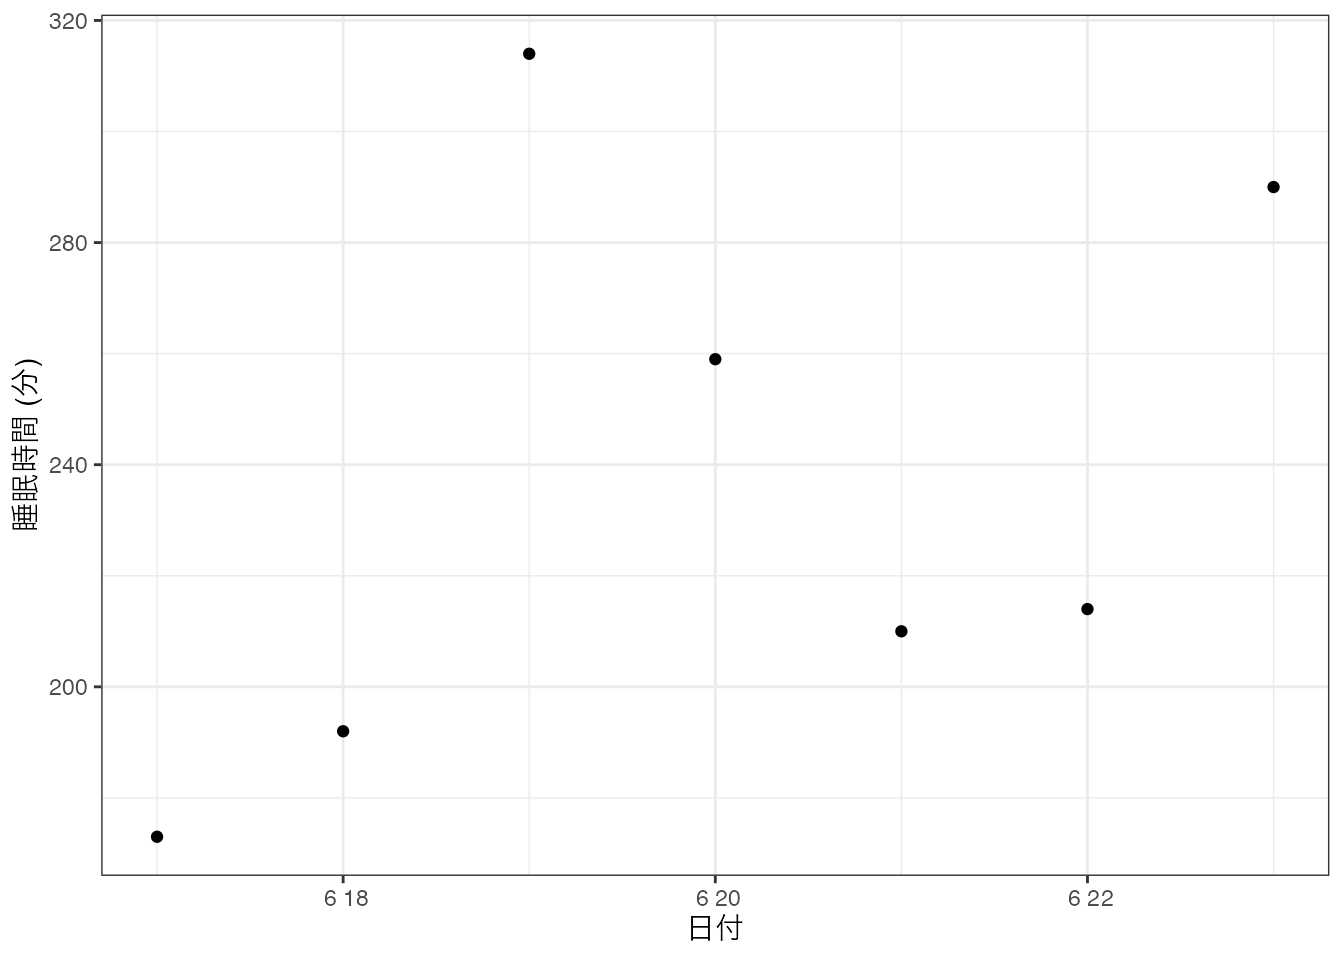
\includegraphics{./datatype_files/figure-pdf/fig-sleep2-1.png}

}

\caption{\label{fig-sleep2}Songの睡眠時間}

\end{figure}

しかし、Songがうっかり6月19日に記録するのを忘れたとします。つまり、\texttt{SongSleep}データの3行目が抜けている状況を考えてみましょう。データフレームの要素抽出については第\ref{sec-datastructure_dataframe}章で解説します。

\begin{Shaded}
\begin{Highlighting}[numbers=left,,]
\NormalTok{SongSleep2 }\OtherTok{\textless{}{-}}\NormalTok{ SongSleep[}\SpecialCharTok{{-}}\DecValTok{3}\NormalTok{, ]}
\end{Highlighting}
\end{Shaded}

中身をみると、以下のようになります。\texttt{Date}も\texttt{DateD}も同じように見えます。

\begin{Shaded}
\begin{Highlighting}[numbers=left,,]
\NormalTok{SongSleep2}
\end{Highlighting}
\end{Shaded}

\begin{verbatim}
        Date Sleep      DateD
1 2017-06-17   173 2017-06-17
2 2017-06-18   192 2017-06-18
4 2017-06-20   259 2017-06-20
5 2017-06-21   210 2017-06-21
6 2017-06-22   214 2017-06-22
7 2017-06-23   290 2017-06-23
\end{verbatim}

この状態で横軸を\texttt{Date}にしたらどうなるでしょうか(
図~\ref{fig-sleep3} )。

\begin{figure}

{\centering 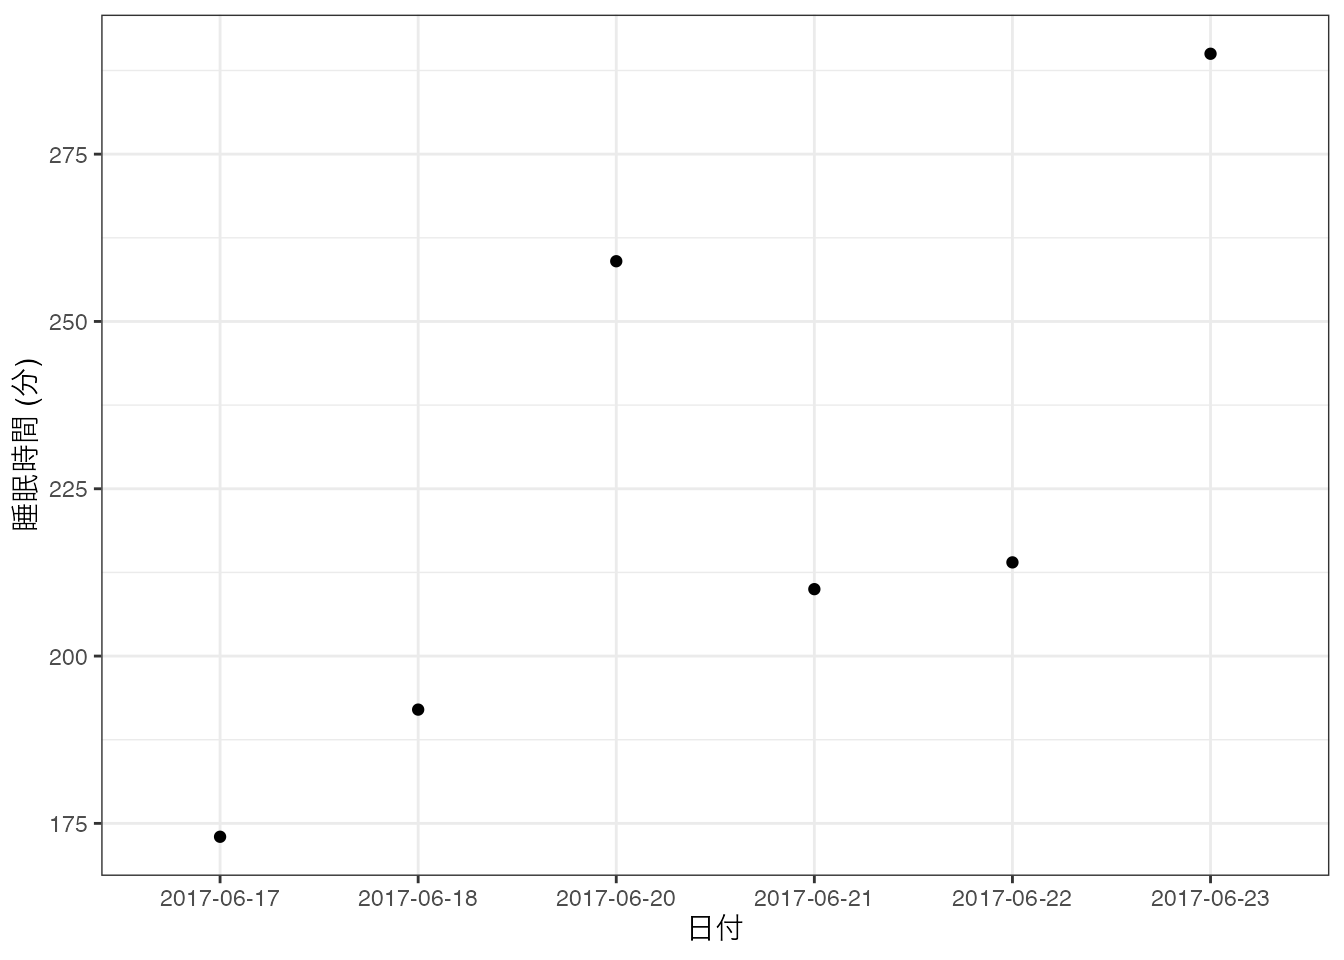
\includegraphics{./datatype_files/figure-pdf/fig-sleep3-1.png}

}

\caption{\label{fig-sleep3}Songの睡眠時間}

\end{figure}

一方、横軸を\texttt{DateD}にしたものが 図~\ref{fig-sleep4} です。

\begin{figure}

{\centering 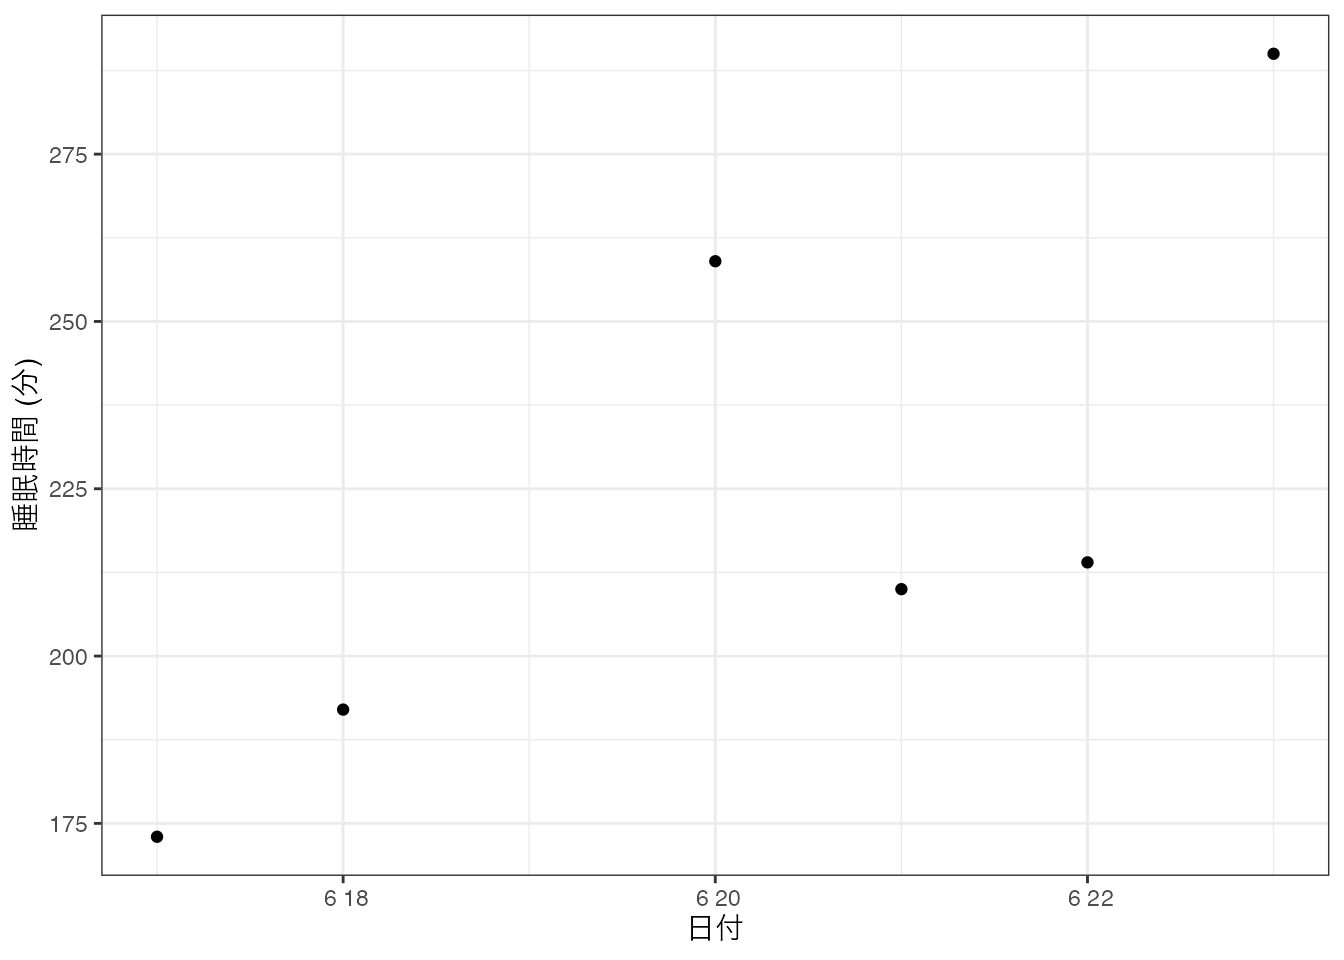
\includegraphics{./datatype_files/figure-pdf/fig-sleep4-1.png}

}

\caption{\label{fig-sleep4}Songの睡眠時間}

\end{figure}

違いが分かりますかね。違いは抜けている6月19日です。 図~\ref{fig-sleep3}
を見ると、横軸の6月18日の次が20日になっています。一方、
図~\ref{fig-sleep4}
は19日になっており、ちゃんと空けてくれますね。これはDate型でない場合、データにないものは図に表示されないことを意味します。一方、Date型は抜けている日があっても、図に表示表示されます。一般のcharacter型またはfactor型でこのようなことを再現するためには、6月19日の列を追加し、睡眠時間を欠損値として指定する必要があります。たとえば、\texttt{SongSleep}データにおいて6月19日の行は温存したまま、睡眠時間だけを欠損値にしてみましょう。

\begin{Shaded}
\begin{Highlighting}[numbers=left,,]
\NormalTok{SongSleep3 }\OtherTok{\textless{}{-}}\NormalTok{ SongSleep}
\NormalTok{SongSleep3}\SpecialCharTok{$}\NormalTok{Sleep[SongSleep}\SpecialCharTok{$}\NormalTok{Date }\SpecialCharTok{==} \StringTok{"2017{-}06{-}19"}\NormalTok{] }\OtherTok{\textless{}{-}} \ConstantTok{NA}

\NormalTok{SongSleep3}
\end{Highlighting}
\end{Shaded}

\begin{verbatim}
        Date Sleep      DateD
1 2017-06-17   173 2017-06-17
2 2017-06-18   192 2017-06-18
3 2017-06-19    NA 2017-06-19
4 2017-06-20   259 2017-06-20
5 2017-06-21   210 2017-06-21
6 2017-06-22   214 2017-06-22
7 2017-06-23   290 2017-06-23
\end{verbatim}

このように日付はあるが、睡眠時間が欠損している場合、図にしたものが
図~\ref{fig-sleep5} です。

\begin{verbatim}
Warning: Removed 1 rows containing missing values (geom_point).
\end{verbatim}

\begin{figure}

{\centering 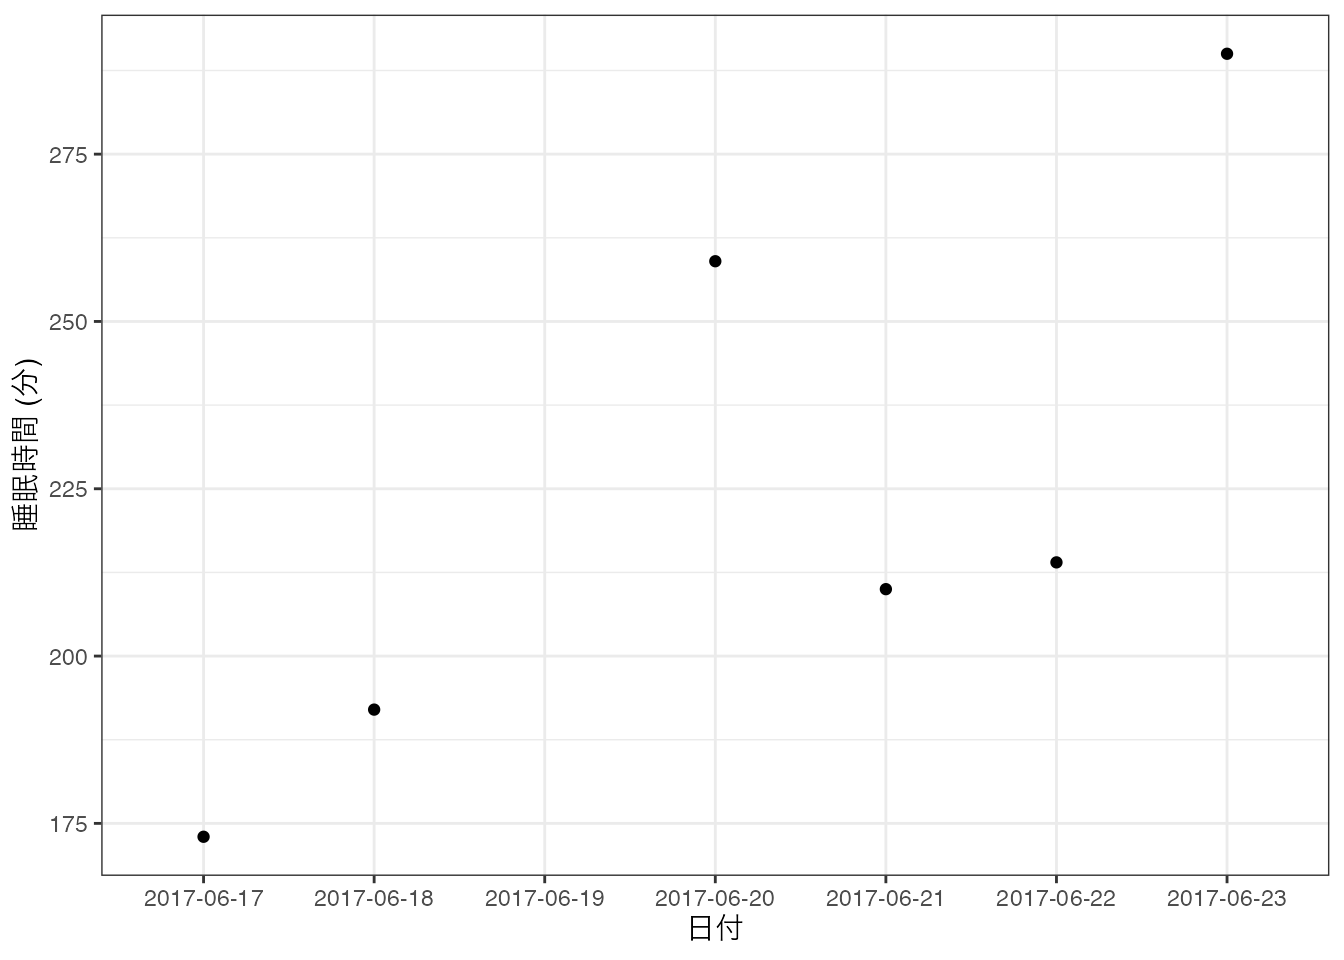
\includegraphics{./datatype_files/figure-pdf/fig-sleep5-1.png}

}

\caption{\label{fig-sleep5}Songの睡眠時間}

\end{figure}

警告が表示されましたが、横軸上に6月19日が表示されます。このようにDate型でなくてもDate型と同じように動かすことは可能ですが、非常に面倒です。その意味でDate型は時系列データを扱う際に非常に便利なデータ型です。

\hypertarget{dateux578bux306eux4f5cux308aux65b9}{%
\subsection{Date型の作り方}\label{dateux578bux306eux4f5cux308aux65b9}}

Date型を作成方法はいくつかあります。

\begin{enumerate}
\def\labelenumi{\arabic{enumi}.}
\tightlist
\item
  character型をDate型にする
\item
  numeric型をDate型にする
\end{enumerate}

主に使う方法は1であり、既に前節でお見せしました\texttt{as.Date()}関数を使います。方法2もまた\texttt{as.Date()}を使いますが、これは「xxxx年xx月xx日から何日目」という書き方となり、起点となる日付
(\texttt{origin})\footnote{主に使う\texttt{origin}は1970年1月1日です。}を指定する必要があります。

ここでは方法1について解説します。日付を表すいくつかのベクトルを作ってみましょう。

\begin{Shaded}
\begin{Highlighting}[numbers=left,,]
\NormalTok{Date1 }\OtherTok{\textless{}{-}} \StringTok{"2020{-}05{-}21"}
\NormalTok{Date2 }\OtherTok{\textless{}{-}} \StringTok{"2020{-}5{-}21"}
\NormalTok{Date3 }\OtherTok{\textless{}{-}} \StringTok{"2020/5/21"}
\NormalTok{Date4 }\OtherTok{\textless{}{-}} \StringTok{"20/05/21"}
\NormalTok{Date5 }\OtherTok{\textless{}{-}} \StringTok{"20200521"}
\NormalTok{Date6 }\OtherTok{\textless{}{-}} \StringTok{"2020 05 21"}
\NormalTok{Date7 }\OtherTok{\textless{}{-}} \StringTok{"2020.05.21"}
\end{Highlighting}
\end{Shaded}

\begin{Shaded}
\begin{Highlighting}[numbers=left,,]
\FunctionTok{as.Date}\NormalTok{(Date1)}
\end{Highlighting}
\end{Shaded}

\begin{verbatim}
[1] "2020-05-21"
\end{verbatim}

\begin{Shaded}
\begin{Highlighting}[numbers=left,,]
\FunctionTok{as.Date}\NormalTok{(Date2)}
\end{Highlighting}
\end{Shaded}

\begin{verbatim}
[1] "2020-05-21"
\end{verbatim}

\begin{Shaded}
\begin{Highlighting}[numbers=left,,]
\FunctionTok{as.Date}\NormalTok{(Date3)}
\end{Highlighting}
\end{Shaded}

\begin{verbatim}
[1] "2020-05-21"
\end{verbatim}

\begin{Shaded}
\begin{Highlighting}[numbers=left,,]
\FunctionTok{as.Date}\NormalTok{(Date4, }\StringTok{"\%y/\%m/\%d"}\NormalTok{)}
\end{Highlighting}
\end{Shaded}

\begin{verbatim}
[1] "2020-05-21"
\end{verbatim}

\begin{Shaded}
\begin{Highlighting}[numbers=left,,]
\FunctionTok{as.Date}\NormalTok{(Date5, }\StringTok{"\%Y\%m\%d"}\NormalTok{)}
\end{Highlighting}
\end{Shaded}

\begin{verbatim}
[1] "2020-05-21"
\end{verbatim}

\begin{Shaded}
\begin{Highlighting}[numbers=left,,]
\FunctionTok{as.Date}\NormalTok{(Date6, }\StringTok{"\%Y \%m \%d"}\NormalTok{)}
\end{Highlighting}
\end{Shaded}

\begin{verbatim}
[1] "2020-05-21"
\end{verbatim}

\begin{Shaded}
\begin{Highlighting}[numbers=left,,]
\FunctionTok{as.Date}\NormalTok{(Date7, }\StringTok{"\%Y.\%m.\%d"}\NormalTok{)}
\end{Highlighting}
\end{Shaded}

\begin{verbatim}
[1] "2020-05-21"
\end{verbatim}

\texttt{Date1}、\texttt{Date2}、\texttt{Date3}のようなベクトルの場合、\texttt{as.Date()}のみでDate型に変換できます。つまり、日付が数字のみで構成され、年が4桁となっており、年月日が\texttt{-}または\texttt{/}で区切られている場合はこれでだけで十分です。しかし、年が2桁になっていたり、その他の記号が使われたり、区切られていない場合は、\texttt{fotmat\ =}引数を指定する必要があります。たとえば\texttt{Date4}は年が2桁となっているます。2桁の年は\texttt{\%y}と表記します。この表記法の一部を以下の表で紹介します。

\begin{longtable}[]{@{}lll@{}}
\toprule
表記 & 説明 & 例 \\
\midrule
\endhead
\%y & 年 (2桁) & 20 \\
\%Y & 年 (4桁) & 2020 \\
\%m & 月 (数字) & 5, 10 \\
\%b & 月 (文字) & Jan \\
\%B & 月 (文字) & January \\
\%d & 日 & 5, 05, 13 \\
\bottomrule
\end{longtable}

他にも様々な表記法がありますが、詳細は\texttt{?strptime}で確認してみてください。

他にも、日本では使わない表記法ですが、月を英語で表記したり、日月年の順で表記する場合があります。後者は\texttt{format\ =}引数の順番を変えるだけで問題有りませんが、問題は前者です。そこで使うのが\texttt{\%b}または\texttt{\%B}です。\texttt{\%b}は3文字の月表記で、\texttt{\%B}はフルネームです。

\begin{Shaded}
\begin{Highlighting}[numbers=left,,]
\FunctionTok{as.Date}\NormalTok{(}\StringTok{"21may2020"}\NormalTok{,   }\AttributeTok{format =} \StringTok{"\%d\%b\%Y"}\NormalTok{)}
\end{Highlighting}
\end{Shaded}

\begin{verbatim}
[1] "2020-05-21"
\end{verbatim}

\begin{Shaded}
\begin{Highlighting}[numbers=left,,]
\FunctionTok{as.Date}\NormalTok{(}\StringTok{"May/21/2020"}\NormalTok{, }\AttributeTok{format =} \StringTok{"\%b/\%d/\%Y"}\NormalTok{)}
\end{Highlighting}
\end{Shaded}

\begin{verbatim}
[1] "2020-05-21"
\end{verbatim}

うまくいかないですね。これはシステムの時間ロケールが日本になっているのが原因です。ロケール設定は\texttt{Sys.getlocale()}で確認できます。

\begin{Shaded}
\begin{Highlighting}[numbers=left,,]
\FunctionTok{Sys.getlocale}\NormalTok{(}\AttributeTok{category =} \StringTok{"LC\_TIME"}\NormalTok{)}
\end{Highlighting}
\end{Shaded}

\begin{verbatim}
[1] "en_US.UTF-8"
\end{verbatim}

これを\texttt{Sys.setlocale()}を使って、\texttt{"C"}に変更します。

\begin{Shaded}
\begin{Highlighting}[numbers=left,,]
\FunctionTok{Sys.setlocale}\NormalTok{(}\AttributeTok{category =} \StringTok{"LC\_TIME"}\NormalTok{, }\AttributeTok{locale =} \StringTok{"C"}\NormalTok{)}
\end{Highlighting}
\end{Shaded}

\begin{verbatim}
[1] "C"
\end{verbatim}

それではもう一回やってみましょう。

\begin{Shaded}
\begin{Highlighting}[numbers=left,,]
\FunctionTok{as.Date}\NormalTok{(}\StringTok{"21may2020"}\NormalTok{,   }\AttributeTok{format =} \StringTok{"\%d\%b\%Y"}\NormalTok{)}
\end{Highlighting}
\end{Shaded}

\begin{verbatim}
[1] "2020-05-21"
\end{verbatim}

\begin{Shaded}
\begin{Highlighting}[numbers=left,,]
\FunctionTok{as.Date}\NormalTok{(}\StringTok{"May/21/2020"}\NormalTok{, }\AttributeTok{format =} \StringTok{"\%b/\%d/\%Y"}\NormalTok{)}
\end{Highlighting}
\end{Shaded}

\begin{verbatim}
[1] "2020-05-21"
\end{verbatim}

うまく動くことが確認できました。念の為に、ロケールを戻しておきます。

\begin{Shaded}
\begin{Highlighting}[numbers=left,,]
\FunctionTok{Sys.setlocale}\NormalTok{(}\AttributeTok{category =} \StringTok{"LC\_TIME"}\NormalTok{, }\AttributeTok{locale =} \StringTok{"ja\_JP.UTF{-}8"}\NormalTok{)}
\end{Highlighting}
\end{Shaded}

\begin{verbatim}
[1] "ja_JP.UTF-8"
\end{verbatim}

\hypertarget{posixctposixltux578bux306bux3064ux3044ux3066}{%
\subsection{POSIXct、POSIXlt型について}\label{posixctposixltux578bux306bux3064ux3044ux3066}}

POSIXct、POSIXlt型は日付だけでなく時間の情報も含むデータ型です。これらは\texttt{as.POSIXct()}、\texttt{as.POSIXlt()}関数で作成することができます。どちらも見た目は同じデータ型ですが、内部構造がことなります\footnote{POSIXct型は基準日
  (1970年1月1日 00時00分00秒 =
  UNIX時間)からの符号付き経過秒数であり、POSIXlt型は日付、時間などがそれぞれ数字として格納されています。可読性の観点からはPOSIXlt型が優れていますが、データ処理の観点から見るとPOSIXct型の方が優れていると言われます。}。詳細は\texttt{?as.POSIXct}または\texttt{?as.POSIXlt}を参照してください。

\begin{center}\rule{0.5\linewidth}{0.5pt}\end{center}

\hypertarget{sec-type_na}{%
\section{NA}\label{sec-type_na}}

NAは欠損値と呼ばれます。これは本来は値があるはずなのがなんらかの理由で欠損していることを意味します。
表~\ref{tbl-na_example1} の例を考えてみましょう。

\hypertarget{tbl-na_example1}{}
\begin{table}
\caption{\label{tbl-na_example1}4人の支持政党 }

\centering
\begin{tabular}{r|l|l|l}
\hline
ID & 名前 & 支持政党あり & 政党名\\
\hline
1 & Yanai & ない & NA\\
\hline
2 & Song & ある & ラーメン大好き党\\
\hline
3 & Shigemura & ある & 鹿児島第一党\\
\hline
4 & Tani & ない & NA\\
\hline
\end{tabular}
\end{table}

3列目で支持政党があるケースのみ、4列目に値があります。YanaiとTaniの場合、支持する政党がないため、政治政党名が欠損しています。実際、多くのデータには欠損値が含まれています。世論調査データの場合はもっと多いです。理由としては「Q2で''はい''を選んだ場合のみQ3に進み、それ以外はQ4へ飛ばす」のようなのもありますが、単に回答を拒否した場合もあります。

まずは欠損値が含まれたベクトル\texttt{NA.Vec1}を作ってみましょう。

\begin{Shaded}
\begin{Highlighting}[numbers=left,,]
\NormalTok{NA.Vec1 }\OtherTok{\textless{}{-}} \FunctionTok{c}\NormalTok{(}\DecValTok{1}\NormalTok{, }\ConstantTok{NA}\NormalTok{, }\DecValTok{3}\NormalTok{, }\ConstantTok{NA}\NormalTok{, }\DecValTok{5}\NormalTok{, }\DecValTok{6}\NormalTok{)}
\NormalTok{NA.Vec1}
\end{Highlighting}
\end{Shaded}

\begin{verbatim}
[1]  1 NA  3 NA  5  6
\end{verbatim}

つづいて、データ型を確認してみましょう。

\begin{Shaded}
\begin{Highlighting}[numbers=left,,]
\FunctionTok{class}\NormalTok{(NA.Vec1)}
\end{Highlighting}
\end{Shaded}

\begin{verbatim}
[1] "numeric"
\end{verbatim}

NAが含まれていてもデータ型はnumericのままです。これは「一応、欠損しているが、ここに何らかの値が割り当てられるとしたらそれはnumeric型だろう」とRが判断しているからです。ある要素がNAか否かを判定するには\texttt{is.na()}関数を使います。

\begin{Shaded}
\begin{Highlighting}[numbers=left,,]
\FunctionTok{is.na}\NormalTok{(NA.Vec1)}
\end{Highlighting}
\end{Shaded}

\begin{verbatim}
[1] FALSE  TRUE FALSE  TRUE FALSE FALSE
\end{verbatim}

2番目と4番目の要素が欠損していることが分かります。

欠損値も要素の一つとしてカウントされるため、ベクトルの長さは6になります。ベクトルの長さは\texttt{length()}関数で確認できます。

\begin{Shaded}
\begin{Highlighting}[numbers=left,,]
\FunctionTok{length}\NormalTok{(NA.Vec1)}
\end{Highlighting}
\end{Shaded}

\begin{verbatim}
[1] 6
\end{verbatim}

\textbf{欠損値の取り扱い}

欠損値を含むデータの処理方法はやや特殊です。まず、\texttt{NA.Vec1}の要素全てに1を足してみましょう。

\begin{Shaded}
\begin{Highlighting}[numbers=left,,]
\NormalTok{NA.Vec1 }\SpecialCharTok{+} \DecValTok{1}
\end{Highlighting}
\end{Shaded}

\begin{verbatim}
[1]  2 NA  4 NA  6  7
\end{verbatim}

この場合、欠損値の箇所には1が足されず、それ以外の要素のみに1を足した結果が返ってきます。これは直感的に考えると自然です。問題になるのは欠損値が含まれるベクトルを関数に入れた場合です。たとえば、numeric型ベクトル内の要素の総和を求めるには\texttt{sum()}関数を使います。\texttt{sum(c(1,\ 3,\ 5))}を入力すると9が返されます。\texttt{NA.Vec1}は欠損していない要素が1,
3, 5, 6であるため、総和は15のはずです。確認してみましょう。

\begin{Shaded}
\begin{Highlighting}[numbers=left,,]
\FunctionTok{sum}\NormalTok{(NA.Vec1)}
\end{Highlighting}
\end{Shaded}

\begin{verbatim}
[1] NA
\end{verbatim}

このように欠損値を含むベクトルの総和はNAとなります。もし、欠損値を除いた要素の総和を求めるには、まずベクトルから欠損値を除去する必要があります。そのためには\texttt{is.na()}関数を使って\texttt{NA.Vec1}の要素を抽出します。ただし、\texttt{is.na()}を使うと、欠損値であるところが\texttt{TRUE}になるため、これを反転する必要があります。この場合は\texttt{!is.na()}関数を使います。それでは\texttt{is.na()}と\texttt{!is.na()}を使って要素を抽出してみましょう。

\begin{Shaded}
\begin{Highlighting}[numbers=left,,]
\NormalTok{NA.Vec1[}\FunctionTok{is.na}\NormalTok{(NA.Vec1)]}
\end{Highlighting}
\end{Shaded}

\begin{verbatim}
[1] NA NA
\end{verbatim}

\begin{Shaded}
\begin{Highlighting}[numbers=left,,]
\NormalTok{NA.Vec1[}\SpecialCharTok{!}\FunctionTok{is.na}\NormalTok{(NA.Vec1)]}
\end{Highlighting}
\end{Shaded}

\begin{verbatim}
[1] 1 3 5 6
\end{verbatim}

\texttt{!is.na()}を使うことで欠損値を除いた要素のみを取り出すことができました。これなら\texttt{sum()}関数も使えるでしょう。

\begin{Shaded}
\begin{Highlighting}[numbers=left,,]
\FunctionTok{sum}\NormalTok{(NA.Vec1[}\SpecialCharTok{!}\FunctionTok{is.na}\NormalTok{(NA.Vec1)])}
\end{Highlighting}
\end{Shaded}

\begin{verbatim}
[1] 15
\end{verbatim}

これで欠損値を除いた要素の総和を求めることができました。ただし、一部の関数には欠損値を自動的に除去するオプションを持つ場合があります。\texttt{sum()}関数のその一部であり、\texttt{na.rm\ =\ TRUE}オプションを付けると、欠損値を除いた総和を返します。

\begin{Shaded}
\begin{Highlighting}[numbers=left,,]
\FunctionTok{sum}\NormalTok{(NA.Vec1, }\AttributeTok{na.rm =} \ConstantTok{TRUE}\NormalTok{)}
\end{Highlighting}
\end{Shaded}

\begin{verbatim}
[1] 15
\end{verbatim}

\textbf{欠損値の使い方}

主に欠損値を扱うのは入手したデータに含まれる欠損値に対してですが、NAをこちらから生成することもあります。それは空ベクトルを用意する時です。第\ref{sec-programming}章では関数の作り方について解説します。関数内で何らかの処理を行い、その結果を返すことになりますが、その結果を格納するベクトルを事前に作っておくこともできます。こちらの方がメモリの観点からは効率的です。以下は第\ref{sec-programming}章を読んでから読んでも構いません。

もし、長さ10のベクトル\texttt{Result.Vec1}を返すとします。ベクトルの要素として1から10の数字が入るとします。一つ目の方法としてはまず、\texttt{Result.Vec1}に1を代入し、次は\texttt{c()}を使って要素を一つずつ足して行く手順です。

\begin{Shaded}
\begin{Highlighting}[numbers=left,,]
\NormalTok{Result.Vec1 }\OtherTok{\textless{}{-}} \DecValTok{1}
\NormalTok{Result.Vec1 }\OtherTok{\textless{}{-}} \FunctionTok{c}\NormalTok{(Result.Vec1, }\DecValTok{2}\NormalTok{)}
\NormalTok{Result.Vec1 }\OtherTok{\textless{}{-}} \FunctionTok{c}\NormalTok{(Result.Vec1, }\DecValTok{3}\NormalTok{)}
\NormalTok{Result.Vec1 }\OtherTok{\textless{}{-}} \FunctionTok{c}\NormalTok{(Result.Vec1, }\DecValTok{4}\NormalTok{)}
\NormalTok{Result.Vec1 }\OtherTok{\textless{}{-}} \FunctionTok{c}\NormalTok{(Result.Vec1, }\DecValTok{5}\NormalTok{)}
\NormalTok{Result.Vec1 }\OtherTok{\textless{}{-}} \FunctionTok{c}\NormalTok{(Result.Vec1, }\DecValTok{6}\NormalTok{)}
\NormalTok{Result.Vec1 }\OtherTok{\textless{}{-}} \FunctionTok{c}\NormalTok{(Result.Vec1, }\DecValTok{7}\NormalTok{)}
\NormalTok{Result.Vec1 }\OtherTok{\textless{}{-}} \FunctionTok{c}\NormalTok{(Result.Vec1, }\DecValTok{8}\NormalTok{)}
\NormalTok{Result.Vec1 }\OtherTok{\textless{}{-}} \FunctionTok{c}\NormalTok{(Result.Vec1, }\DecValTok{9}\NormalTok{)}
\NormalTok{Result.Vec1 }\OtherTok{\textless{}{-}} \FunctionTok{c}\NormalTok{(Result.Vec1, }\DecValTok{10}\NormalTok{)}
\end{Highlighting}
\end{Shaded}

二つ目の方法はまず、10個のNAが格納されたベクトル\texttt{Reuslt.Vec2}を作っておいて、その中に要素を置換してく方法です。

\begin{Shaded}
\begin{Highlighting}[numbers=left,,]
\NormalTok{Result.Vec2     }\OtherTok{\textless{}{-}} \FunctionTok{rep}\NormalTok{(}\ConstantTok{NA}\NormalTok{, }\DecValTok{10}\NormalTok{)}
\NormalTok{Result.Vec2[}\DecValTok{1}\NormalTok{]  }\OtherTok{\textless{}{-}} \DecValTok{1}
\NormalTok{Result.Vec2[}\DecValTok{2}\NormalTok{]  }\OtherTok{\textless{}{-}} \DecValTok{2}
\NormalTok{Result.Vec2[}\DecValTok{3}\NormalTok{]  }\OtherTok{\textless{}{-}} \DecValTok{3}
\NormalTok{Result.Vec2[}\DecValTok{4}\NormalTok{]  }\OtherTok{\textless{}{-}} \DecValTok{4}
\NormalTok{Result.Vec2[}\DecValTok{5}\NormalTok{]  }\OtherTok{\textless{}{-}} \DecValTok{5}
\NormalTok{Result.Vec2[}\DecValTok{6}\NormalTok{]  }\OtherTok{\textless{}{-}} \DecValTok{6}
\NormalTok{Result.Vec2[}\DecValTok{7}\NormalTok{]  }\OtherTok{\textless{}{-}} \DecValTok{7}
\NormalTok{Result.Vec2[}\DecValTok{8}\NormalTok{]  }\OtherTok{\textless{}{-}} \DecValTok{8}
\NormalTok{Result.Vec2[}\DecValTok{9}\NormalTok{]  }\OtherTok{\textless{}{-}} \DecValTok{9}
\NormalTok{Result.Vec2[}\DecValTok{10}\NormalTok{] }\OtherTok{\textless{}{-}} \DecValTok{10}
\end{Highlighting}
\end{Shaded}

以上の手順を\texttt{for()}を使って反復処理するとしたら、以下のようなコードになります。

\begin{Shaded}
\begin{Highlighting}[numbers=left,,]
\CommentTok{\# 方法1}
\NormalTok{Result.Vec1 }\OtherTok{\textless{}{-}} \DecValTok{1}

\ControlFlowTok{for}\NormalTok{ (i }\ControlFlowTok{in} \DecValTok{2}\SpecialCharTok{:}\DecValTok{10}\NormalTok{) \{}
\NormalTok{    Result.Vec1 }\OtherTok{\textless{}{-}} \FunctionTok{c}\NormalTok{(Result.Vec1, i)}
\NormalTok{\}}

\CommentTok{\# 方法2}
\NormalTok{Result.Vec2 }\OtherTok{\textless{}{-}} \FunctionTok{rep}\NormalTok{(}\ConstantTok{NA}\NormalTok{, }\DecValTok{10}\NormalTok{)}

\ControlFlowTok{for}\NormalTok{ (i }\ControlFlowTok{in} \DecValTok{1}\SpecialCharTok{:}\DecValTok{10}\NormalTok{) \{}
\NormalTok{    Result.Vec2[i] }\OtherTok{\textless{}{-}}\NormalTok{ i}
\NormalTok{\}}
\end{Highlighting}
\end{Shaded}

結果を確認してみましょう。

\begin{Shaded}
\begin{Highlighting}[numbers=left,,]
\NormalTok{Result.Vec1}
\end{Highlighting}
\end{Shaded}

\begin{verbatim}
 [1]  1  2  3  4  5  6  7  8  9 10
\end{verbatim}

\begin{Shaded}
\begin{Highlighting}[numbers=left,,]
\NormalTok{Result.Vec2}
\end{Highlighting}
\end{Shaded}

\begin{verbatim}
 [1]  1  2  3  4  5  6  7  8  9 10
\end{verbatim}

コードの書き方は異なりますが、どれも結果は同じです。また、どちらが早いかというと、これくらいの計算ならどの方法でも同じです。ただし、より大規模の反復作業を行う場合、後者の方が時間が節約でき、コードの可読性も高いです。

\begin{center}\rule{0.5\linewidth}{0.5pt}\end{center}

\hypertarget{sec-type_null}{%
\section{NULL}\label{sec-type_null}}

NULLは「存在しない」、空っぽであることを意味します。先ほどのNAはデータは存在するはずなのに、何らかの理由で値が存在しない、または割り当てられていないことを意味しますが、NULLは「存在しません」。したがって、NULLが含まれたベクトルを作成しても表示されません。NULLが含まれた\texttt{NULL.Vec1}を作ってみましょう。

\begin{Shaded}
\begin{Highlighting}[numbers=left,,]
\NormalTok{NULL.Vec1 }\OtherTok{\textless{}{-}} \FunctionTok{c}\NormalTok{(}\DecValTok{1}\NormalTok{, }\DecValTok{3}\NormalTok{, }\ConstantTok{NULL}\NormalTok{, }\DecValTok{5}\NormalTok{, }\DecValTok{10}\NormalTok{)}
\NormalTok{NULL.Vec1}
\end{Highlighting}
\end{Shaded}

\begin{verbatim}
[1]  1  3  5 10
\end{verbatim}

3番目の要素であるNULLは表示されません。ということはNAと違って、データの長さも5ではなく4でしょう。確認してみます。

\begin{Shaded}
\begin{Highlighting}[numbers=left,,]
\FunctionTok{length}\NormalTok{(NULL.Vec1)}
\end{Highlighting}
\end{Shaded}

\begin{verbatim}
[1] 4
\end{verbatim}

この\texttt{NULL.Vec1}のデータ型は何でしょう。

\begin{Shaded}
\begin{Highlighting}[numbers=left,,]
\FunctionTok{class}\NormalTok{(NULL.Vec1)}
\end{Highlighting}
\end{Shaded}

\begin{verbatim}
[1] "numeric"
\end{verbatim}

\texttt{is.null()}関数もありますが、どうでしょうか。

\begin{Shaded}
\begin{Highlighting}[numbers=left,,]
\FunctionTok{is.null}\NormalTok{(NULL.Vec1)}
\end{Highlighting}
\end{Shaded}

\begin{verbatim}
[1] FALSE
\end{verbatim}

NULLは存在しないことを意味するため、\texttt{NULL.Vec1}は要素が4のnumeric型ベクトルです。\texttt{is.null()}でNULLが判定できるのは\texttt{is.null(NULL)}のようなケースです。このNULLはいつ使うのでしょうか。実際、使う機会はあまりありません。強いて言えば、空っぽのリストを作成する際に使うケースがあります。リストについては第\ref{sec-datastructure}章で説明します。以下の例は第\ref{sec-datastructure}章を読み終わってから目を通して下さい。

\begin{Shaded}
\begin{Highlighting}[numbers=left,,]
\NormalTok{NULL.List1 }\OtherTok{\textless{}{-}} \FunctionTok{list}\NormalTok{(}\AttributeTok{Room1 =} \DecValTok{1}\SpecialCharTok{:}\DecValTok{3}\NormalTok{,}
                   \AttributeTok{Room2 =} \FunctionTok{c}\NormalTok{(}\StringTok{"Yuki"}\NormalTok{, }\StringTok{"Jaehyun"}\NormalTok{, }\StringTok{"Hadley"}\NormalTok{),}
                   \AttributeTok{Room3 =} \ConstantTok{NULL}\NormalTok{)}

\NormalTok{NULL.List1}
\end{Highlighting}
\end{Shaded}

\begin{verbatim}
$Room1
[1] 1 2 3

$Room2
[1] "Yuki"    "Jaehyun" "Hadley" 

$Room3
NULL
\end{verbatim}

このように予めリストの要素は作っておきたいが、とりあえず空けておく際に使います。続く分析の段階で\texttt{NULL.List1{[}{[}"Room3"{]}{]}}に何かを格納したりすることに使えるでしょう。ちなみにこの場合は\texttt{is.null()}が使用可能です。

\begin{Shaded}
\begin{Highlighting}[numbers=left,,]
\FunctionTok{is.null}\NormalTok{(NULL.List1[[}\StringTok{"Room3"}\NormalTok{]])}
\end{Highlighting}
\end{Shaded}

\begin{verbatim}
[1] TRUE
\end{verbatim}

\begin{center}\rule{0.5\linewidth}{0.5pt}\end{center}

\hypertarget{sec-type_nan}{%
\section{NaN}\label{sec-type_nan}}

NaNはnumeric型、中でもdouble型の一種ですが、これは計算できない値を意味します。つまり、NaN値を直接入力することはめったにありませんが、計算の結果として\texttt{NaN}が返されるケースがあります。代表的な例が0を0で割った場合です。実際、0を0で割ることはできません。ここでは0を0で割った値を含む\texttt{NaN.Vec1}作ってみましょう。

\begin{Shaded}
\begin{Highlighting}[numbers=left,,]
\NormalTok{NaN.Vec1 }\OtherTok{\textless{}{-}} \FunctionTok{c}\NormalTok{(}\DecValTok{2}\SpecialCharTok{/}\DecValTok{5}\NormalTok{, }\DecValTok{0}\SpecialCharTok{/}\DecValTok{12}\NormalTok{, }\DecValTok{0}\SpecialCharTok{/}\DecValTok{0}\NormalTok{)}
\NormalTok{NaN.Vec1}
\end{Highlighting}
\end{Shaded}

\begin{verbatim}
[1] 0.4 0.0 NaN
\end{verbatim}

\begin{Shaded}
\begin{Highlighting}[numbers=left,,]
\FunctionTok{class}\NormalTok{(NaN.Vec1)}
\end{Highlighting}
\end{Shaded}

\begin{verbatim}
[1] "numeric"
\end{verbatim}

先ほどせつめいしましたように、NaNはnumeric型の一部ですので、データ型としてはnumeircになります。ある値がNaNか否かを判定するには\texttt{is.nan()}関数を使います。

\begin{Shaded}
\begin{Highlighting}[numbers=left,,]
\FunctionTok{is.nan}\NormalTok{(NaN.Vec1)}
\end{Highlighting}
\end{Shaded}

\begin{verbatim}
[1] FALSE FALSE  TRUE
\end{verbatim}

\begin{center}\rule{0.5\linewidth}{0.5pt}\end{center}

\hypertarget{sec-type_inf}{%
\section{Inf}\label{sec-type_inf}}

Infもまたnumeric型、中でもdouble型の一部ですが、これは無限大を意味します。Infも通常、自分から作成するケースはあまりなく、結果として帰ってくる場合があります。一つの例が0以外の数値を0で割った場合です。それではなんらかの数値を0を割った値が含まれるベクトル\texttt{Inf.Vec1}を作ってみましょう。

\begin{Shaded}
\begin{Highlighting}[numbers=left,,]
\NormalTok{Inf.Vec1 }\OtherTok{\textless{}{-}} \FunctionTok{c}\NormalTok{(}\DecValTok{28}\SpecialCharTok{/}\DecValTok{95}\NormalTok{, }\DecValTok{3}\SpecialCharTok{/}\DecValTok{0}\NormalTok{, }\SpecialCharTok{{-}}\DecValTok{12}\SpecialCharTok{/}\DecValTok{0}\NormalTok{, }\DecValTok{0}\SpecialCharTok{/}\DecValTok{0}\NormalTok{)}
\NormalTok{Inf.Vec1}
\end{Highlighting}
\end{Shaded}

\begin{verbatim}
[1] 0.2947368       Inf      -Inf       NaN
\end{verbatim}

\begin{Shaded}
\begin{Highlighting}[numbers=left,,]
\FunctionTok{class}\NormalTok{(Inf.Vec1)}
\end{Highlighting}
\end{Shaded}

\begin{verbatim}
[1] "numeric"
\end{verbatim}

正の値を0で割ったら\texttt{Inf}が負の値を0で割ったら\texttt{-Inf}が返ってきます。これは正の無限大、負の無限大を意味します。データ型はNaNと同様、numeric型ですが、\texttt{is.infinite()}を使うと、無限大か否かが判定できます。

\begin{Shaded}
\begin{Highlighting}[numbers=left,,]
\FunctionTok{is.infinite}\NormalTok{(Inf.Vec1)}
\end{Highlighting}
\end{Shaded}

\begin{verbatim}
[1] FALSE  TRUE  TRUE FALSE
\end{verbatim}

\hypertarget{sec-datastructure}{%
\chapter{データ構造}\label{sec-datastructure}}

\hypertarget{sec-datastructure_intro}{%
\section{データ構造とは}\label{sec-datastructure_intro}}

データ構造 (data
structure)とは最小単位であるベクトルを何らかの形で集めたものです。ベクトル自体もデータ構造であり、同じデータ型のベクトルを積み重ねた行列、異なるデータ型の縦ベクトルを横に並べたデータフレームなど、Rでは様々なデータ構造を提供しています。また、R内臓のデータ構造以外にも、パッケージ等で提供される独自のデータ構造もあります。ここではRが基本的に提供している代表的なデータ構造について、その作り方と操作方法について解説します。

\begin{center}\rule{0.5\linewidth}{0.5pt}\end{center}

\hypertarget{sec-datastructure_vector}{%
\section{ベクトル (vector)}\label{sec-datastructure_vector}}

\hypertarget{ux30d9ux30afux30c8ux30ebux306eux4f5cux308aux65b9}{%
\subsection{ベクトルの作り方}\label{ux30d9ux30afux30c8ux30ebux306eux4f5cux308aux65b9}}

Rにおいてベクトルとは\textbf{同じデータ型が一つ以上格納されているオブジェクト}を意味します。たとえば、以下の\texttt{myVec1}は長さ1のベクトルです。

\begin{Shaded}
\begin{Highlighting}[numbers=left,,]
\NormalTok{myVec1 }\OtherTok{\textless{}{-}} \StringTok{"R is fun!"}
\NormalTok{myVec1}
\end{Highlighting}
\end{Shaded}

\begin{verbatim}
[1] "R is fun!"
\end{verbatim}

むろん、2つ以上の文字列、または数字を格納することも可能です。以下の\texttt{myVec2}は長さ5のベクトルです。

\begin{Shaded}
\begin{Highlighting}[numbers=left,,]
\NormalTok{myVec2 }\OtherTok{\textless{}{-}} \FunctionTok{c}\NormalTok{(}\DecValTok{1}\NormalTok{, }\DecValTok{3}\NormalTok{, }\DecValTok{5}\NormalTok{, }\DecValTok{6}\NormalTok{, }\DecValTok{7}\NormalTok{)}
\NormalTok{myVec2}
\end{Highlighting}
\end{Shaded}

\begin{verbatim}
[1] 1 3 5 6 7
\end{verbatim}

注意すべきところは、ベクトル内の要素は必ず同じデータ型である必要があるということです。たとえば、数字と文字が混在した\texttt{myVec3}を考えてみましょう。

\begin{Shaded}
\begin{Highlighting}[numbers=left,,]
\NormalTok{myVec3 }\OtherTok{\textless{}{-}} \FunctionTok{c}\NormalTok{(}\StringTok{"A"}\NormalTok{, }\StringTok{"B"}\NormalTok{, }\StringTok{"C"}\NormalTok{, }\DecValTok{1}\NormalTok{, }\DecValTok{2}\NormalTok{, }\DecValTok{3}\NormalTok{)}
\NormalTok{myVec3}
\end{Highlighting}
\end{Shaded}

\begin{verbatim}
[1] "A" "B" "C" "1" "2" "3"
\end{verbatim}

数字であるはずの1, 2,
3が\texttt{"}で囲まれ、文字列に自動的に変換されていることが分かります。実際に、デーが型を確認してみましょう。

\begin{Shaded}
\begin{Highlighting}[numbers=left,,]
\FunctionTok{class}\NormalTok{(myVec3)}
\end{Highlighting}
\end{Shaded}

\begin{verbatim}
[1] "character"
\end{verbatim}

\texttt{"character"}、つまりデータ型が文字列になっていることが分かります。これは\texttt{character}型が\texttt{numeric}型よりも優先順位が高いからです。それでは\texttt{numeric}と\texttt{logical}型はどうでしょうか。

\begin{Shaded}
\begin{Highlighting}[numbers=left,,]
\NormalTok{myVec4 }\OtherTok{\textless{}{-}} \FunctionTok{c}\NormalTok{(}\DecValTok{1}\NormalTok{, }\DecValTok{2}\NormalTok{, }\DecValTok{3}\NormalTok{, }\ConstantTok{TRUE}\NormalTok{, }\ConstantTok{FALSE}\NormalTok{)}
\NormalTok{myVec4}
\end{Highlighting}
\end{Shaded}

\begin{verbatim}
[1] 1 2 3 1 0
\end{verbatim}

\begin{Shaded}
\begin{Highlighting}[numbers=left,,]
\FunctionTok{class}\NormalTok{(myVec4)}
\end{Highlighting}
\end{Shaded}

\begin{verbatim}
[1] "numeric"
\end{verbatim}

\texttt{TRUE}が1、\texttt{FALSE}が0となり、自動的に\texttt{numeric}型になりました。一般的によく使われるデータ型は\texttt{logical}、\texttt{numeric}、\texttt{character}ですが、優先順位は\texttt{logical\ \textless{}\ numeric\ \textless{}\ character}の関係になります。ここで重要なのは優先順位ではなく、異なるデータ型が含まれるベクトルの場合、自動的にデータ型が統一されるということです。ベクトルを作成する際は、全ての要素が同じ型になるようにしましょう。

\hypertarget{ux30d9ux30afux30c8ux30ebux306eux64cdux4f5c}{%
\subsection{ベクトルの操作}\label{ux30d9ux30afux30c8ux30ebux306eux64cdux4f5c}}

\textbf{ベクトルの長さ}

ベクトルの長さはベクトルに含まれている要素の数です。ベクトルの長さは\texttt{length()}関数で調べることができます。それでは前節で作成した4つのベクトルの長さを調べてみましょう。

\begin{Shaded}
\begin{Highlighting}[numbers=left,,]
\FunctionTok{length}\NormalTok{(myVec1) }\CommentTok{\# "R is fun!"}
\end{Highlighting}
\end{Shaded}

\begin{verbatim}
[1] 1
\end{verbatim}

\begin{Shaded}
\begin{Highlighting}[numbers=left,,]
\FunctionTok{length}\NormalTok{(myVec2) }\CommentTok{\# c(1, 3, 5, 6, 7)}
\end{Highlighting}
\end{Shaded}

\begin{verbatim}
[1] 5
\end{verbatim}

\begin{Shaded}
\begin{Highlighting}[numbers=left,,]
\FunctionTok{length}\NormalTok{(myVec3) }\CommentTok{\# c("A", "B", "C", "1", "2", "3")}
\end{Highlighting}
\end{Shaded}

\begin{verbatim}
[1] 6
\end{verbatim}

\begin{Shaded}
\begin{Highlighting}[numbers=left,,]
\FunctionTok{length}\NormalTok{(myVec4) }\CommentTok{\# c(1, 2, 3, 1, 0)}
\end{Highlighting}
\end{Shaded}

\begin{verbatim}
[1] 5
\end{verbatim}

それぞれのベクトルの長さは1、5、6、5ということが分かりますね。

\textbf{要素の抽出}

これは既に説明しましたので、第\ref{sec-rbasic_extract}を参照してください。

\textbf{ベクトルの加減乗除}

ここではnumeric型のベクトルを用いた加減乗除について考えたいと思います。Rにおいてベクトルは自動的に反復作業を行います。たとえば、\texttt{c(1,\ 2,\ 3,\ 4)}というベクトルがあり、ここに5を足すと、ベクトルの全ての要素に対して同じ計算を行います。これは引き算でも、掛け算でも、割り算でも同じです。むろん、べき乗などの様々な操作に対しても同じです。それでは\texttt{myVec2}に対して、5を足したり、引いたり、色々してみましょう。

\begin{Shaded}
\begin{Highlighting}[numbers=left,,]
\NormalTok{myVec2 }\SpecialCharTok{+} \DecValTok{5}
\end{Highlighting}
\end{Shaded}

\begin{verbatim}
[1]  6  8 10 11 12
\end{verbatim}

\begin{Shaded}
\begin{Highlighting}[numbers=left,,]
\NormalTok{myVec2 }\SpecialCharTok{{-}} \DecValTok{5}
\end{Highlighting}
\end{Shaded}

\begin{verbatim}
[1] -4 -2  0  1  2
\end{verbatim}

\begin{Shaded}
\begin{Highlighting}[numbers=left,,]
\NormalTok{myVec2 }\SpecialCharTok{*} \DecValTok{5}
\end{Highlighting}
\end{Shaded}

\begin{verbatim}
[1]  5 15 25 30 35
\end{verbatim}

\begin{Shaded}
\begin{Highlighting}[numbers=left,,]
\NormalTok{myVec2 }\SpecialCharTok{/} \DecValTok{5}
\end{Highlighting}
\end{Shaded}

\begin{verbatim}
[1] 0.2 0.6 1.0 1.2 1.4
\end{verbatim}

\begin{Shaded}
\begin{Highlighting}[numbers=left,,]
\NormalTok{myVec2 }\SpecialCharTok{\^{}} \DecValTok{5}
\end{Highlighting}
\end{Shaded}

\begin{verbatim}
[1]     1   243  3125  7776 16807
\end{verbatim}

また、ベクトル同士の演算も可能です。まず、\texttt{myVec2}と同じ長さを持つ\texttt{myVec4}との計算を考えてみましょう。これは長さが同じであるため、それぞれ同じ位置の要素同士の計算となります。つまり、足し算の場合、\texttt{myVec2{[}1{]}}と\texttt{myVec4{[}1{]}}の和、\texttt{myVec2{[}2{]}}と\texttt{myVec4{[}2{]}}の和、\ldots といった形です。

\begin{Shaded}
\begin{Highlighting}[numbers=left,,]
\NormalTok{myVec2 }\SpecialCharTok{+}\NormalTok{ myVec4}
\end{Highlighting}
\end{Shaded}

\begin{verbatim}
[1] 2 5 8 7 7
\end{verbatim}

\begin{Shaded}
\begin{Highlighting}[numbers=left,,]
\NormalTok{myVec2 }\SpecialCharTok{{-}}\NormalTok{ myVec4}
\end{Highlighting}
\end{Shaded}

\begin{verbatim}
[1] 0 1 2 5 7
\end{verbatim}

\begin{Shaded}
\begin{Highlighting}[numbers=left,,]
\NormalTok{myVec2 }\SpecialCharTok{*}\NormalTok{ myVec4}
\end{Highlighting}
\end{Shaded}

\begin{verbatim}
[1]  1  6 15  6  0
\end{verbatim}

\begin{Shaded}
\begin{Highlighting}[numbers=left,,]
\NormalTok{myVec2 }\SpecialCharTok{/}\NormalTok{ myVec4}
\end{Highlighting}
\end{Shaded}

\begin{verbatim}
[1] 1.000000 1.500000 1.666667 6.000000      Inf
\end{verbatim}

もし、ベクトルの長さが異なる場合はどうなるでしょう。たとえば、長さ2のベクトル\texttt{myVec5}と\texttt{myVec2}の足し算を考えてみましょう。

\begin{Shaded}
\begin{Highlighting}[numbers=left,,]
\NormalTok{(myVec5 }\OtherTok{\textless{}{-}} \FunctionTok{c}\NormalTok{(}\DecValTok{1}\NormalTok{, }\DecValTok{10}\NormalTok{))}
\end{Highlighting}
\end{Shaded}

\begin{verbatim}
[1]  1 10
\end{verbatim}

\begin{Shaded}
\begin{Highlighting}[numbers=left,,]
\NormalTok{(myVec6 }\OtherTok{\textless{}{-}}\NormalTok{ myVec2 }\SpecialCharTok{+}\NormalTok{ myVec5)}
\end{Highlighting}
\end{Shaded}

\begin{verbatim}
Warning in myVec2 + myVec5: longer object length is not a multiple of shorter
object length
\end{verbatim}

\begin{verbatim}
[1]  2 13  6 16  8
\end{verbatim}

警告メッセージは表示されますが、計算自体はできます。同じ長さのベクトル同士なら、同じ位置の要素同士の計算になりますが、この場合は、短い方のベクトルを繰り返すことにより、長さを合わせることになります。\texttt{myVec5}の例だと、\texttt{c(1,\ 10,\ 1,\ 10,\ 1)}のように扱われます。具体的には以下の表のような関係となります。

\begin{longtable}[]{@{}ccccc@{}}
\toprule
\texttt{myVec6{[}1{]}} & \texttt{myVec6{[}2{]}} & \texttt{myVec6{[}3{]}}
& \texttt{myVec6{[}4{]}} & \texttt{myVec6{[}5{]}} \\
\midrule
\endhead
\texttt{myVec2{[}1{]}} & \texttt{myVec2{[}2{]}} & \texttt{myVec2{[}3{]}}
& \texttt{myVec2{[}4{]}} & \texttt{myVec2{[}5{]}} \\
+ & + & + & + & + \\
\texttt{myVec5{[}1{]}} & \texttt{myVec5{[}2{]}} & \texttt{myVec5{[}1{]}}
& \texttt{myVec5{[}2{]}} & \texttt{myVec5{[}1{]}} \\
\bottomrule
\end{longtable}

実際は長さが異なるベクトル同士の計算を行うことは滅多にありません。例外としては長さ1のベクトルの計算くらいですね。

文字列ベクトルの扱い方はより複雑ですので、第\ref{sec-string}章で詳細に解説します。

\begin{center}\rule{0.5\linewidth}{0.5pt}\end{center}

\hypertarget{sec-datastructure_matrix}{%
\section{行列 (matrix)}\label{sec-datastructure_matrix}}

行列は名前とおり、行と列で構成されたデータ構造です。ただし、我々が一般に考える「表」とは異なる点があります。それは行列内部の要素に制約がある点です。具体的に、行列の要素となり得るデータ型はnumeric、complex、NA型のみです。ここではnumeric型のみで構成された行列の作成および操作方法について解説します。

\hypertarget{ux884cux5217ux306eux4f5cux308aux65b9}{%
\subsection{行列の作り方}\label{ux884cux5217ux306eux4f5cux308aux65b9}}

行列を作成するには\texttt{matrix()}関数を使います。引数として、行列に入る数値と行または列の数は必須です。数値はベクトルであり、行・列の数は整数です。以下のような行列を作るにはいくつかの方法があります。

\[
\left[
\begin{matrix} 
1 & 2 & 3 & 4 \\ 
5 & 6 & 7 & 8 \\
9 & 10 & 11 & 12
\end{matrix}
\right]
\]

\begin{Shaded}
\begin{Highlighting}[numbers=left,,]
\CommentTok{\# 方法1: 行数を指定する}
\NormalTok{Matrix1 }\OtherTok{\textless{}{-}} \FunctionTok{matrix}\NormalTok{(}\FunctionTok{c}\NormalTok{(}\DecValTok{1}\NormalTok{, }\DecValTok{5}\NormalTok{, }\DecValTok{9}\NormalTok{, }\DecValTok{2}\NormalTok{, }\DecValTok{6}\NormalTok{, }\DecValTok{10}\NormalTok{, }\DecValTok{3}\NormalTok{, }\DecValTok{7}\NormalTok{, }\DecValTok{11}\NormalTok{, }\DecValTok{4}\NormalTok{, }\DecValTok{8}\NormalTok{, }\DecValTok{12}\NormalTok{), }\AttributeTok{nrow =} \DecValTok{3}\NormalTok{)}
\NormalTok{Matrix1}
\end{Highlighting}
\end{Shaded}

\begin{verbatim}
     [,1] [,2] [,3] [,4]
[1,]    1    2    3    4
[2,]    5    6    7    8
[3,]    9   10   11   12
\end{verbatim}

\begin{Shaded}
\begin{Highlighting}[numbers=left,,]
\CommentTok{\# 方法2: 列数を指定する}
\NormalTok{Matrix2 }\OtherTok{\textless{}{-}} \FunctionTok{matrix}\NormalTok{(}\FunctionTok{c}\NormalTok{(}\DecValTok{1}\NormalTok{, }\DecValTok{5}\NormalTok{, }\DecValTok{9}\NormalTok{, }\DecValTok{2}\NormalTok{, }\DecValTok{6}\NormalTok{, }\DecValTok{10}\NormalTok{, }\DecValTok{3}\NormalTok{, }\DecValTok{7}\NormalTok{, }\DecValTok{11}\NormalTok{, }\DecValTok{4}\NormalTok{, }\DecValTok{8}\NormalTok{, }\DecValTok{12}\NormalTok{), }\AttributeTok{ncol =} \DecValTok{4}\NormalTok{)}
\NormalTok{Matrix2}
\end{Highlighting}
\end{Shaded}

\begin{verbatim}
     [,1] [,2] [,3] [,4]
[1,]    1    2    3    4
[2,]    5    6    7    8
[3,]    9   10   11   12
\end{verbatim}

いずれも同じ結果が得られます。注意してもらいたいところは、第一引数の書き方です。我々は「左から右へ、そして上から下へ」という順番で読むのになれていますが、\textbf{Rの行列は「上から下へ、そして左から右へ」の順番}です。もし、「左から右へ、そして上から下へ」のような、より我々にとって読みやすい書き方をするためにはもう一つの引数が必要であり、それが\texttt{byrow\ =}です。

\begin{Shaded}
\begin{Highlighting}[numbers=left,,]
\NormalTok{(}\FunctionTok{matrix}\NormalTok{(}\FunctionTok{c}\NormalTok{(}\DecValTok{1}\NormalTok{, }\DecValTok{2}\NormalTok{, }\DecValTok{3}\NormalTok{, }\DecValTok{4}\NormalTok{, }\DecValTok{5}\NormalTok{, }\DecValTok{6}\NormalTok{, }\DecValTok{7}\NormalTok{, }\DecValTok{8}\NormalTok{, }\DecValTok{9}\NormalTok{, }\DecValTok{10}\NormalTok{, }\DecValTok{11}\NormalTok{, }\DecValTok{12}\NormalTok{), }\AttributeTok{nrow =} \DecValTok{3}\NormalTok{, }\AttributeTok{byrow =} \ConstantTok{TRUE}\NormalTok{))}
\end{Highlighting}
\end{Shaded}

\begin{verbatim}
     [,1] [,2] [,3] [,4]
[1,]    1    2    3    4
[2,]    5    6    7    8
[3,]    9   10   11   12
\end{verbatim}

むろん、初項1、公差1、最大値12の等差数列ですのて、\texttt{1:12}のような書き方も可能です。

\begin{Shaded}
\begin{Highlighting}[numbers=left,,]
\NormalTok{(}\FunctionTok{matrix}\NormalTok{(}\DecValTok{1}\SpecialCharTok{:}\DecValTok{12}\NormalTok{, }\AttributeTok{nrow =} \DecValTok{3}\NormalTok{, }\AttributeTok{byrow =} \ConstantTok{TRUE}\NormalTok{))}
\end{Highlighting}
\end{Shaded}

\begin{verbatim}
     [,1] [,2] [,3] [,4]
[1,]    1    2    3    4
[2,]    5    6    7    8
[3,]    9   10   11   12
\end{verbatim}

データ構造も確認してみましょう。

\begin{Shaded}
\begin{Highlighting}[numbers=left,,]
\FunctionTok{class}\NormalTok{(Matrix1)}
\end{Highlighting}
\end{Shaded}

\begin{verbatim}
[1] "matrix" "array" 
\end{verbatim}

R
4.0.0からの仕様変更により行列型はmatrix構造以外にもarrayの構造も持つようになりました。array型については第\ref{sec-datastructure_array}章で解説します。

\textbf{単位行列}

最後にちょっと特殊な行列である単位行列 (indetity
matrix)の作り方について説明します。単位行列とは行と列の数が同じである正方形の行列ですが、対角線上は全て1、その他は全て0となっている行列です。たとえば大きさが4の単位行列は、

\[
\left[
\begin{matrix} 
1 & 0 & 0 & 0 \\ 
0 & 1 & 0 & 0 \\ 
0 & 0 & 1 & 0 \\ 
0 & 0 & 0 & 1 \\ 
\end{matrix}
\right]
\]

です。これは\texttt{matrix(c(1,\ 0,\ 0,\ 0,\ 0,\ 1,\ 0,\ 0,\ 0,\ 0,\ 1,\ 0,\ 0,\ 0,\ 0,\ 1),\ nrow\ =\ 4)}で作成することも可能ですが、\texttt{diag()}関数を使えば簡単に出来ます。サイズが4の単位行列は\texttt{diag(4)}です。

\begin{Shaded}
\begin{Highlighting}[numbers=left,,]
\NormalTok{(}\FunctionTok{diag}\NormalTok{(}\DecValTok{4}\NormalTok{))}
\end{Highlighting}
\end{Shaded}

\begin{verbatim}
     [,1] [,2] [,3] [,4]
[1,]    1    0    0    0
[2,]    0    1    0    0
[3,]    0    0    1    0
[4,]    0    0    0    1
\end{verbatim}

\hypertarget{ux884cux5217ux306eux64cdux4f5c}{%
\subsection{行列の操作}\label{ux884cux5217ux306eux64cdux4f5c}}

まず、以下のような行列\texttt{A}を作ってみましょう。

\[
A = \left[
\begin{matrix} 
1 & 2 & 3 & 4 \\ 
5 & 6 & 7 & 8 \\
9 & 10 & 11 & 12
\end{matrix}
\right]
\]

\begin{Shaded}
\begin{Highlighting}[numbers=left,,]
\NormalTok{A }\OtherTok{\textless{}{-}} \FunctionTok{matrix}\NormalTok{(}\FunctionTok{c}\NormalTok{(}\DecValTok{1}\NormalTok{, }\DecValTok{2}\NormalTok{, }\DecValTok{3}\NormalTok{, }\DecValTok{4}\NormalTok{, }\DecValTok{5}\NormalTok{, }\DecValTok{6}\NormalTok{, }\DecValTok{7}\NormalTok{, }\DecValTok{8}\NormalTok{, }\DecValTok{9}\NormalTok{, }\DecValTok{10}\NormalTok{, }\DecValTok{11}\NormalTok{, }\DecValTok{12}\NormalTok{), }
            \AttributeTok{nrow =} \DecValTok{3}\NormalTok{, }\AttributeTok{byrow =} \ConstantTok{TRUE}\NormalTok{)}
\end{Highlighting}
\end{Shaded}

\textbf{行列のサイズ}

行列の大きさ (行と列の数)を求める際は\texttt{dim()}関数を使います。

\begin{Shaded}
\begin{Highlighting}[numbers=left,,]
\FunctionTok{dim}\NormalTok{(A)}
\end{Highlighting}
\end{Shaded}

\begin{verbatim}
[1] 3 4
\end{verbatim}

結果は長さ2のベクトルですが、1番目の要素が行数、2番目の要素が列数になります。もし、行列の行数のみ確認したい場合は\texttt{dim(A){[}1{]}}、列数なら\texttt{dim(A){[}2{]}}で確認することができます。また、全く同じ機能を持つ関数があり、それが\texttt{nrow()}と\texttt{ncol()}関数です。

\begin{Shaded}
\begin{Highlighting}[numbers=left,,]
\FunctionTok{nrow}\NormalTok{(A) }\CommentTok{\# 行列の行数を確認: dim(A)[1]と同じ}
\end{Highlighting}
\end{Shaded}

\begin{verbatim}
[1] 3
\end{verbatim}

\begin{Shaded}
\begin{Highlighting}[numbers=left,,]
\FunctionTok{ncol}\NormalTok{(A) }\CommentTok{\# 列列の列数を確認: dim(A)[2]と同じ}
\end{Highlighting}
\end{Shaded}

\begin{verbatim}
[1] 4
\end{verbatim}

\texttt{dim()}および\texttt{nrow()}、\texttt{ncol()}関数は第\ref{sec-datastructure_dataframe}章で紹介するデータフレームでも使用可能です。

\textbf{要素の抽出}

ベクトルと同様、要素の抽出は\texttt{{[}{]}}を使います。ただし、行列は横と縦の2次元構成となりますので、行と列のそれぞれの位置を指定する必要があります。たとえば、\texttt{A}の2行目、3列目の要素を抽出するためには、

\begin{Shaded}
\begin{Highlighting}[numbers=left,,]
\NormalTok{A[}\DecValTok{2}\NormalTok{, }\DecValTok{3}\NormalTok{]}
\end{Highlighting}
\end{Shaded}

\begin{verbatim}
[1] 7
\end{verbatim}

のように書きます。行か列の位置を省略した場合、指定した列・行全てが抽出されます。2行目の要素全てを抽出するなら\texttt{A{[}2,\ {]}}、3列目の要素全てを抽出するなら\texttt{A{[},\ 3{]}}となります。

\begin{Shaded}
\begin{Highlighting}[numbers=left,,]
\NormalTok{A[}\DecValTok{2}\NormalTok{, ]}
\end{Highlighting}
\end{Shaded}

\begin{verbatim}
[1] 5 6 7 8
\end{verbatim}

\begin{Shaded}
\begin{Highlighting}[numbers=left,,]
\NormalTok{A[, }\DecValTok{3}\NormalTok{]}
\end{Highlighting}
\end{Shaded}

\begin{verbatim}
[1]  3  7 11
\end{verbatim}

この場合、返される値のデータ構造はいずれも\textbf{行列でなく、ベクトル}です。確認してみましょう。

\begin{Shaded}
\begin{Highlighting}[numbers=left,,]
\FunctionTok{is.vector}\NormalTok{(A[}\DecValTok{2}\NormalTok{, }\DecValTok{3}\NormalTok{])}
\end{Highlighting}
\end{Shaded}

\begin{verbatim}
[1] TRUE
\end{verbatim}

\begin{Shaded}
\begin{Highlighting}[numbers=left,,]
\FunctionTok{is.vector}\NormalTok{(A[}\DecValTok{2}\NormalTok{, ])}
\end{Highlighting}
\end{Shaded}

\begin{verbatim}
[1] TRUE
\end{verbatim}

\begin{Shaded}
\begin{Highlighting}[numbers=left,,]
\FunctionTok{is.vector}\NormalTok{(A[, }\DecValTok{3}\NormalTok{])}
\end{Highlighting}
\end{Shaded}

\begin{verbatim}
[1] TRUE
\end{verbatim}

例外は複数の行と複数の列を同時に抽出した場合です。たとえば、行列\texttt{A}の1・2行目と2・3列目の要素を全て抽出するとします。その場合は\texttt{A{[}1:2,\ 2:3{]}}のように書きます。むろん、\texttt{:}を使わずに\texttt{A{[}c(1,\ 2),\ c(2,\ 3){]}}のような書き方も可能です。抽出後、返された結果のデータ構造も確認してみましょう。

\begin{Shaded}
\begin{Highlighting}[numbers=left,,]
\NormalTok{A[}\DecValTok{1}\SpecialCharTok{:}\DecValTok{2}\NormalTok{, }\DecValTok{3}\SpecialCharTok{:}\DecValTok{4}\NormalTok{]}
\end{Highlighting}
\end{Shaded}

\begin{verbatim}
     [,1] [,2]
[1,]    3    4
[2,]    7    8
\end{verbatim}

\begin{Shaded}
\begin{Highlighting}[numbers=left,,]
\FunctionTok{class}\NormalTok{(A[}\DecValTok{1}\SpecialCharTok{:}\DecValTok{2}\NormalTok{, }\DecValTok{3}\SpecialCharTok{:}\DecValTok{4}\NormalTok{])}
\end{Highlighting}
\end{Shaded}

\begin{verbatim}
[1] "matrix" "array" 
\end{verbatim}

この場合、返された結果のデータ構造は行列であることが分かります。

\textbf{行列の足し算と引き算}

行列の足し算 (引き算)には

\begin{enumerate}
\def\labelenumi{\arabic{enumi}.}
\tightlist
\item
  行列内の全要素に対して同じ数字を足す (引く)
\item
  同じサイズの2つの行列から対応する要素を足す (引く)
\end{enumerate}

2パタンがあります。例えば、行列\texttt{A}の全要素に5を足す場合は以下のように入力します。

\begin{Shaded}
\begin{Highlighting}[numbers=left,,]
\NormalTok{(A\_plus\_5 }\OtherTok{\textless{}{-}}\NormalTok{ A }\SpecialCharTok{+} \DecValTok{5}\NormalTok{)}
\end{Highlighting}
\end{Shaded}

\begin{verbatim}
     [,1] [,2] [,3] [,4]
[1,]    6    7    8    9
[2,]   10   11   12   13
[3,]   14   15   16   17
\end{verbatim}

同様に、\texttt{A}から10を引く場合は\texttt{-}演算子を使います。

\begin{Shaded}
\begin{Highlighting}[numbers=left,,]
\NormalTok{(A\_minus\_10 }\OtherTok{\textless{}{-}}\NormalTok{ A }\SpecialCharTok{{-}} \DecValTok{10}\NormalTok{)}
\end{Highlighting}
\end{Shaded}

\begin{verbatim}
     [,1] [,2] [,3] [,4]
[1,]   -9   -8   -7   -6
[2,]   -5   -4   -3   -2
[3,]   -1    0    1    2
\end{verbatim}

二つ目は同じサイズの行列同士の足し算と引き算です。行列\texttt{A}は3
\(\times\)
4の行列ですので、同じサイズの行列\texttt{B}を作成してみましょう。

\begin{Shaded}
\begin{Highlighting}[numbers=left,,]
\NormalTok{(B }\OtherTok{\textless{}{-}} \FunctionTok{matrix}\NormalTok{(}\FunctionTok{c}\NormalTok{(}\DecValTok{3}\NormalTok{, }\DecValTok{2}\NormalTok{, }\DecValTok{1}\NormalTok{, }\DecValTok{4}\NormalTok{, }\DecValTok{5}\NormalTok{, }\DecValTok{9}\NormalTok{, }\DecValTok{7}\NormalTok{, }\DecValTok{11}\NormalTok{, }\DecValTok{6}\NormalTok{, }\DecValTok{12}\NormalTok{, }\DecValTok{8}\NormalTok{, }\DecValTok{10}\NormalTok{), }
             \AttributeTok{nrow =} \DecValTok{3}\NormalTok{, }\AttributeTok{byrow =} \ConstantTok{TRUE}\NormalTok{))}
\end{Highlighting}
\end{Shaded}

\begin{verbatim}
     [,1] [,2] [,3] [,4]
[1,]    3    2    1    4
[2,]    5    9    7   11
[3,]    6   12    8   10
\end{verbatim}

この行列\texttt{A}と\texttt{B}の足し算はそれぞれ同じ位置の要素同士の和を行列をして返し、これは引き算も同じです。

\begin{Shaded}
\begin{Highlighting}[numbers=left,,]
\NormalTok{A }\SpecialCharTok{+}\NormalTok{ B}
\end{Highlighting}
\end{Shaded}

\begin{verbatim}
     [,1] [,2] [,3] [,4]
[1,]    4    4    4    8
[2,]   10   15   14   19
[3,]   15   22   19   22
\end{verbatim}

\begin{Shaded}
\begin{Highlighting}[numbers=left,,]
\NormalTok{A }\SpecialCharTok{{-}}\NormalTok{ B}
\end{Highlighting}
\end{Shaded}

\begin{verbatim}
     [,1] [,2] [,3] [,4]
[1,]   -2    0    2    0
[2,]    0   -3    0   -3
[3,]    3   -2    3    2
\end{verbatim}

注意すべき点は、2つの行列は同じ大きさでなければならない点です。たとえば、行列\texttt{B}の1列から3列までを抽出した3
\(\times\) 3行列\texttt{C}を作成し、\texttt{A\ +\ C}をしてみましょう。

\begin{Shaded}
\begin{Highlighting}[numbers=left,,]
\NormalTok{(C }\OtherTok{\textless{}{-}}\NormalTok{ B[, }\DecValTok{1}\SpecialCharTok{:}\DecValTok{3}\NormalTok{])}
\end{Highlighting}
\end{Shaded}

\begin{verbatim}
     [,1] [,2] [,3]
[1,]    3    2    1
[2,]    5    9    7
[3,]    6   12    8
\end{verbatim}

\begin{Shaded}
\begin{Highlighting}[numbers=left,,]
\NormalTok{A }\SpecialCharTok{+}\NormalTok{ C}
\end{Highlighting}
\end{Shaded}

\begin{verbatim}
Error in A + C: non-conformable arrays
\end{verbatim}

このように足し算ができなくなり、これは引き算でも同じです。

\textbf{行列の掛け算}

やや特殊なのは行列の掛け算です。行列\texttt{A}の全要素を2倍にしたい場合、これは足し算・引き算と同じやり方で十分です。

\begin{Shaded}
\begin{Highlighting}[numbers=left,,]
\NormalTok{A }\SpecialCharTok{*} \DecValTok{2}
\end{Highlighting}
\end{Shaded}

\begin{verbatim}
     [,1] [,2] [,3] [,4]
[1,]    2    4    6    8
[2,]   10   12   14   16
[3,]   18   20   22   24
\end{verbatim}

ただし、問題は行列同士の掛け算です。行列\texttt{A}と\texttt{B}の掛け算といえば、直感的には足し算や引き算同様、同じ位置の要素の積と考えるかも知れません。実際\texttt{A\ *\ B}はそのように計算を行います。

\begin{Shaded}
\begin{Highlighting}[numbers=left,,]
\NormalTok{A }\SpecialCharTok{*}\NormalTok{ B}
\end{Highlighting}
\end{Shaded}

\begin{verbatim}
     [,1] [,2] [,3] [,4]
[1,]    3    4    3   16
[2,]   25   54   49   88
[3,]   54  120   88  120
\end{verbatim}

ただし、このような掛け算は「アダマール積 (Hadamard
product)」と呼ばれる計算方法であり\footnote{他にも要素ごとの積
  (element-wise product)、シューア積 (Schur product)と呼ばれたりします。}、一般的に使う掛け算ではありません。実際、数学において\(A \times B\)はアダマール積を意味すのではなく、アダマール積は\(A \circ B\)または\(A \odot B\)と表記します。

それでは一般的な行列の積は何でしょう。詳しいことは線形代数の入門書に譲りますが、以下のような2つの行列\texttt{C}と\texttt{D}を考えてみましょう。

\[
C = \left[
\begin{matrix} 
1 & 2 & 3 \\ 
4 & 5 & 6 
\end{matrix}
\right],
D = \left[
\begin{matrix} 
2 & 7  & 17 \\ 
3 & 11 & 19 \\
5 & 13 & 23
\end{matrix}
\right]
\]

行列の大きさが異なりますね。行列\texttt{C}の大きさは2 \(\times\)
3、\texttt{D}は3 \(\times\)
3です。実はこれが正しいです。行列の積は\(n \times m\)の行列と\(m \times p\)の行列同士でないと計算できません。\(n\)と\(p\)は同じでも、同じでなくても構いません。その意味で\(C \times D\)は計算可能でも、\(D \times C\)は計算できません。そして、2つの行列の積の大きさは\(n \times p\)です。したがって、\(C \times D\)の大きさは\(2 \times 3\)です。

行列の積がどのように求められるかを確認するために、まず行列\texttt{C}と\texttt{D}を作成してみましょう。

\begin{Shaded}
\begin{Highlighting}[numbers=left,,]
\NormalTok{(C }\OtherTok{\textless{}{-}} \FunctionTok{matrix}\NormalTok{(}\FunctionTok{c}\NormalTok{(}\DecValTok{1}\NormalTok{, }\DecValTok{2}\NormalTok{, }\DecValTok{3}\NormalTok{, }\DecValTok{4}\NormalTok{, }\DecValTok{5}\NormalTok{, }\DecValTok{6}\NormalTok{), }\AttributeTok{nrow =} \DecValTok{2}\NormalTok{,}\AttributeTok{byrow =} \ConstantTok{TRUE}\NormalTok{))}
\end{Highlighting}
\end{Shaded}

\begin{verbatim}
     [,1] [,2] [,3]
[1,]    1    2    3
[2,]    4    5    6
\end{verbatim}

\begin{Shaded}
\begin{Highlighting}[numbers=left,,]
\NormalTok{(D }\OtherTok{\textless{}{-}} \FunctionTok{matrix}\NormalTok{(}\FunctionTok{c}\NormalTok{(}\DecValTok{2}\NormalTok{, }\DecValTok{7}\NormalTok{, }\DecValTok{17}\NormalTok{, }\DecValTok{3}\NormalTok{, }\DecValTok{11}\NormalTok{, }\DecValTok{19}\NormalTok{, }\DecValTok{5}\NormalTok{, }\DecValTok{13}\NormalTok{, }\DecValTok{23}\NormalTok{), }\AttributeTok{nrow =} \DecValTok{3}\NormalTok{,}\AttributeTok{byrow =} \ConstantTok{TRUE}\NormalTok{))}
\end{Highlighting}
\end{Shaded}

\begin{verbatim}
     [,1] [,2] [,3]
[1,]    2    7   17
[2,]    3   11   19
[3,]    5   13   23
\end{verbatim}

この2つの積は\texttt{\%*\%}演算子で計算されますが、まずその結果から見ましょう。

\begin{Shaded}
\begin{Highlighting}[numbers=left,,]
\NormalTok{(E }\OtherTok{\textless{}{-}}\NormalTok{ C }\SpecialCharTok{\%*\%}\NormalTok{ D)}
\end{Highlighting}
\end{Shaded}

\begin{verbatim}
     [,1] [,2] [,3]
[1,]   23   68  124
[2,]   53  161  301
\end{verbatim}

2行2列の行列ができました。これらの数字、どうやった計算されたのでしょうか。\texttt{E}の\texttt{{[}1,\ 1{]}}は23であり、\texttt{{[}1,\ 2{]}}は68、\texttt{{[}2,\ 1{]}}は53、\texttt{{[}2,\ 2{]}}は161です。各値は以下のように求まります。

\begin{itemize}
\tightlist
\item
  \texttt{E{[}1,\ 1{]}} = (\texttt{C{[}1,\ 1{]}} *
  \texttt{D{[}1,\ 1{]}}) + (\texttt{C{[}1,\ 2{]}} *
  \texttt{D{[}2,\ 1{]}}) + (\texttt{C{[}1,\ 3{]}} *
  \texttt{D{[}3,\ 1{]}}) = 23
\item
  \texttt{E{[}1,\ 2{]}} = (\texttt{C{[}1,\ 1{]}} *
  \texttt{D{[}1,\ 2{]}}) + (\texttt{C{[}1,\ 2{]}} *
  \texttt{D{[}2,\ 2{]}}) + (\texttt{C{[}1,\ 3{]}} *
  \texttt{D{[}3,\ 2{]}}) = 68
\item
  \texttt{E{[}1,\ 3{]}} = (\texttt{C{[}1,\ 1{]}} *
  \texttt{D{[}1,\ 3{]}}) + (\texttt{C{[}1,\ 2{]}} *
  \texttt{D{[}2,\ 3{]}}) + (\texttt{C{[}1,\ 3{]}} *
  \texttt{D{[}3,\ 3{]}}) = 124
\item
  \texttt{E{[}2,\ 1{]}} = (\texttt{C{[}2,\ 1{]}} *
  \texttt{D{[}1,\ 1{]}}) + (\texttt{C{[}2,\ 2{]}} *
  \texttt{D{[}2,\ 1{]}}) + (\texttt{C{[}2,\ 3{]}} *
  \texttt{D{[}3,\ 1{]}}) = 53
\item
  \texttt{E{[}2,\ 2{]}} = (\texttt{C{[}2,\ 1{]}} *
  \texttt{D{[}1,\ 2{]}}) + (\texttt{C{[}2,\ 2{]}} *
  \texttt{D{[}2,\ 2{]}}) + (\texttt{C{[}2,\ 3{]}} *
  \texttt{D{[}3,\ 2{]}}) = 161
\item
  \texttt{E{[}2,\ 3{]}} = (\texttt{C{[}2,\ 1{]}} *
  \texttt{D{[}1,\ 3{]}}) + (\texttt{C{[}2,\ 2{]}} *
  \texttt{D{[}2,\ 3{]}}) + (\texttt{C{[}2,\ 3{]}} *
  \texttt{D{[}3,\ 3{]}}) = 301
\end{itemize}

大きさ\(n \times m\)行列\texttt{C}の\texttt{i}行目\texttt{j}列目の要素を\(C_{i,j}\)と表記し、大きさ\(n \times p\)行列\texttt{D}の\texttt{i}行目\texttt{j}列目の要素を\(D_{i,j}\)と表記した場合、以下のような関係が成り立ちます。

行列\texttt{E}の\texttt{i}行目\texttt{j}列目の要素を\(e_{i,j}\)と表記した場合、以下のような関係が成り立ちます。

\[
e_{i, j} = \sum_{k = 1}^m C_{i, k} \cdot D_{k, j}.
\]

したがって、行列\(C\)と\(D\)の積は

\begin{align} 
CD = E & = \left[
\begin{matrix} 
e_{1, 1} & e_{1, 2} & e_{1, 3} \\ 
e_{2, 1} & e_{2, 2} & e_{2, 3}
\end{matrix}
\right] \\
& = \left[
\begin{matrix} 
\sum_{k = 1}^m C_{1, k} \cdot D_{k, 1} & \sum_{k = 1}^m C_{1, k} \cdot D_{k, 2} & \sum_{k = 1}^m C_{1, k} \cdot D_{k, 3} \\ 
\sum_{k = 1}^m C_{2, k} \cdot D_{k, 1} & \sum_{k = 1}^m C_{2, k} \cdot D_{k, 2} & \sum_{k = 1}^m C_{2, k} \cdot D_{k, 3}
\end{matrix}
\right].
\end{align}

このように業績同士の積はかなり求めるのが面倒ですが、Rを使えば一瞬で終わります。

\textbf{行列式}

行列式
(determinant)は\(n \times n\)の正方行列のみに対して定義される値の一つです。主に一次方程式において解が存在するか否かを判断するために用いられる数値ですが\footnote{行列式が0でない場合において一次方程式には一組の解があります。}、その詳しい意味や求め方については線形代数の入門書を参照してください。

行列\(A\)の行列式は一般的に\(\text{det}(A)\)、または\(|A|\)と表記されます。行列式を求めるRの関数は\texttt{det()}です。それでは適当に正方行列\texttt{F}を作成し、その行列を求めてみましょう。

\begin{Shaded}
\begin{Highlighting}[numbers=left,,]
\NormalTok{(F }\OtherTok{\textless{}{-}} \FunctionTok{matrix}\NormalTok{(}\FunctionTok{c}\NormalTok{(}\DecValTok{2}\NormalTok{, }\SpecialCharTok{{-}}\DecValTok{6}\NormalTok{, }\DecValTok{4}\NormalTok{, }\DecValTok{7}\NormalTok{, }\DecValTok{2}\NormalTok{, }\DecValTok{3}\NormalTok{, }\DecValTok{8}\NormalTok{, }\DecValTok{5}\NormalTok{, }\SpecialCharTok{{-}}\DecValTok{1}\NormalTok{), }\AttributeTok{nrow =} \DecValTok{3}\NormalTok{, }\AttributeTok{byrow =} \DecValTok{3}\NormalTok{))}
\end{Highlighting}
\end{Shaded}

\begin{verbatim}
     [,1] [,2] [,3]
[1,]    2   -6    4
[2,]    7    2    3
[3,]    8    5   -1
\end{verbatim}

\begin{Shaded}
\begin{Highlighting}[numbers=left,,]
\FunctionTok{det}\NormalTok{(F)}
\end{Highlighting}
\end{Shaded}

\begin{verbatim}
[1] -144
\end{verbatim}

行列\texttt{F}の行列式は-144です。この場合、以下の一次方程式に何らかの一組の解が存在することを意味します
(\(p\), \(q\), \(r\)は任意の実数)。

\begin{align}
2x - 6y + 4z = & p, \\
7x + 2y + 3z = & q, \\
8x + 5y - 1z = & r.
\end{align}

しかし、以下のような連立方程式はいかがでしょう。これは二組以上の解が存在する方程式です\footnote{なぜなら2行目が1行目の0.5倍になっているからです。}。

\begin{align}
2x - 6y + 4z = & p, \\
1x - 3y + 2z = & q, \\
5x + 9y + 3z = & r.
\end{align}

実際に行列\texttt{G}を作成し、\texttt{det(G)}を計算してみましょう。

\begin{Shaded}
\begin{Highlighting}[numbers=left,,]
\NormalTok{(G }\OtherTok{\textless{}{-}} \FunctionTok{matrix}\NormalTok{(}\FunctionTok{c}\NormalTok{(}\DecValTok{2}\NormalTok{, }\SpecialCharTok{{-}}\DecValTok{6}\NormalTok{, }\DecValTok{4}\NormalTok{, }\DecValTok{1}\NormalTok{, }\SpecialCharTok{{-}}\DecValTok{3}\NormalTok{, }\DecValTok{2}\NormalTok{, }\DecValTok{5}\NormalTok{, }\DecValTok{9}\NormalTok{, }\DecValTok{3}\NormalTok{), }\AttributeTok{nrow =} \DecValTok{3}\NormalTok{, }\AttributeTok{byrow =} \DecValTok{3}\NormalTok{))}
\end{Highlighting}
\end{Shaded}

\begin{verbatim}
     [,1] [,2] [,3]
[1,]    2   -6    4
[2,]    1   -3    2
[3,]    5    9    3
\end{verbatim}

\begin{Shaded}
\begin{Highlighting}[numbers=left,,]
\FunctionTok{det}\NormalTok{(G)}
\end{Highlighting}
\end{Shaded}

\begin{verbatim}
[1] 0
\end{verbatim}

\(|G|\)は0であることが分かりますね。

\textbf{階数}

行列の特徴を表す代表的な数値の一つが階数
(rank)です。詳しい説明は省きますが、一次方程式の例だと、階数が行列の行数と一致する場合、一組の解が存在することを意味します。階数を求める方法は\texttt{qr(行列)\$rank}であり、行列\texttt{F}と\texttt{G}の階数を確認してみましょう。

\begin{Shaded}
\begin{Highlighting}[numbers=left,,]
\FunctionTok{qr}\NormalTok{(F)}\SpecialCharTok{$}\NormalTok{rank}
\end{Highlighting}
\end{Shaded}

\begin{verbatim}
[1] 3
\end{verbatim}

\begin{Shaded}
\begin{Highlighting}[numbers=left,,]
\FunctionTok{qr}\NormalTok{(G)}\SpecialCharTok{$}\NormalTok{rank}
\end{Highlighting}
\end{Shaded}

\begin{verbatim}
[1] 2
\end{verbatim}

どれも3行の行列ですが、行列\texttt{F}の階数は3、行列\texttt{G}の階数は2です。\texttt{G}の階数は\texttt{G}の行数より小さいため、連立方程式に一組の解がないことが分かります。

階数の活用先は様々であり、行列式とは違って、正方行列でなくても計算可能です。

\textbf{逆行列}

逆行列とは掛け算すると単位行列となる行列を意味します。行列\(A\)の逆行列は一般的に\(A^{\prime}\)と表記し、\(A \times A^{\prime} = I\)となります。この逆行列の求め方は非常に複雑であり、一定以上の大きさの行列になると手計算で解くのはほぼ不可能です。しかし、Rでは逆行列を計算する\texttt{solve()}関数が内蔵されております。

以下の行列\(A\) (\texttt{A})の逆行列、\(A^{\prime}\)
(\texttt{Ap})を求めてみましょう。そして\(A \times A^{\prime}\)が単位行列になるかまで確認してみます。

\begin{Shaded}
\begin{Highlighting}[numbers=left,,]
\CommentTok{\# 行列Aの作成}
\NormalTok{(A  }\OtherTok{\textless{}{-}} \FunctionTok{matrix}\NormalTok{(}\FunctionTok{c}\NormalTok{(}\DecValTok{1}\NormalTok{, }\SpecialCharTok{{-}}\DecValTok{2}\NormalTok{, }\DecValTok{2}\NormalTok{, }\DecValTok{0}\NormalTok{, }\DecValTok{1}\NormalTok{, }\SpecialCharTok{{-}}\DecValTok{1}\NormalTok{, }\DecValTok{1}\NormalTok{, }\DecValTok{0}\NormalTok{, }\DecValTok{1}\NormalTok{), }\AttributeTok{nrow =} \DecValTok{3}\NormalTok{))}
\end{Highlighting}
\end{Shaded}

\begin{verbatim}
     [,1] [,2] [,3]
[1,]    1    0    1
[2,]   -2    1    0
[3,]    2   -1    1
\end{verbatim}

\begin{Shaded}
\begin{Highlighting}[numbers=left,,]
\CommentTok{\# 行列Aの逆行列を計算し、Apに格納}
\NormalTok{(Ap }\OtherTok{\textless{}{-}} \FunctionTok{solve}\NormalTok{(A))}
\end{Highlighting}
\end{Shaded}

\begin{verbatim}
     [,1] [,2] [,3]
[1,]    1   -1   -1
[2,]    2   -1   -2
[3,]    0    1    1
\end{verbatim}

\begin{Shaded}
\begin{Highlighting}[numbers=left,,]
\CommentTok{\# AとApの積が単位行列であることを確認}
\NormalTok{A }\SpecialCharTok{\%*\%}\NormalTok{ Ap}
\end{Highlighting}
\end{Shaded}

\begin{verbatim}
     [,1] [,2] [,3]
[1,]    1    0    0
[2,]    0    1    0
[3,]    0    0    1
\end{verbatim}

ちゃんと単位行列ができましたね。

\textbf{転置}

行列\(A\)の転置行列は\(A^T\)と表記され、以下のような関係となります。

\[
A = \left[
\begin{matrix} 
1 & 2 & 3 \\ 
4 & 5 & 6 \\
7 & 8 & 9
\end{matrix}
\right],
A^T = \left[
\begin{matrix} 
1 & 4 & 7 \\ 
2 & 5 & 8 \\
3 & 6 & 9
\end{matrix}
\right]
\]

正方行列の場合、対角成分を除き、全ての要素が対角成分を中心に反転していることが分かりますね。このような転置行列の作成には\texttt{t()}関数を使います。それでは行列\texttt{A}とその転置行列\texttt{At}を作ってみましょう。

\begin{Shaded}
\begin{Highlighting}[numbers=left,,]
\NormalTok{A  }\OtherTok{\textless{}{-}} \FunctionTok{matrix}\NormalTok{(}\DecValTok{1}\SpecialCharTok{:}\DecValTok{9}\NormalTok{, }\AttributeTok{byrow =} \ConstantTok{TRUE}\NormalTok{, }\AttributeTok{nrow =} \DecValTok{3}\NormalTok{)}
\NormalTok{A}
\end{Highlighting}
\end{Shaded}

\begin{verbatim}
     [,1] [,2] [,3]
[1,]    1    2    3
[2,]    4    5    6
[3,]    7    8    9
\end{verbatim}

\begin{Shaded}
\begin{Highlighting}[numbers=left,,]
\NormalTok{At }\OtherTok{\textless{}{-}} \FunctionTok{t}\NormalTok{(A)}
\end{Highlighting}
\end{Shaded}

ちなみに転置行列は正方行列でなくても作成できます。

\begin{center}\rule{0.5\linewidth}{0.5pt}\end{center}

\hypertarget{sec-datastructure_dataframe}{%
\section{データフレーム
(data.frame)}\label{sec-datastructure_dataframe}}

データフレームはデータ分析の際に最もよく見るデータ構造です。我々が一般的に考える表形式のデータはデータフレームです。行列も見た目は表に近いですが、行列は中身の要素がnumericまたはcomplex型に限定されるに対して\footnote{\texttt{NA}も可能です。}、データフレームはcharacterやfactor、Dateなど様々なデータ型が許容されます。

\hypertarget{ux30c7ux30fcux30bfux30d5ux30ecux30fcux30e0ux306eux4f5cux6210}{%
\subsection{データフレームの作成}\label{ux30c7ux30fcux30bfux30d5ux30ecux30fcux30e0ux306eux4f5cux6210}}

まずは、 表~\ref{tbl-dataframe_example1}
のようなデータフレームを作成して見ましょう。データフレームを作成する際は\texttt{data.frame()}関数を使います。

\begin{table}

\caption{\label{tbl-dataframe_example1}\textbf{?(caption)}}\begin{minipage}[t]{\linewidth}
\subcaption{\label{tbl-dataframe_example1-1}}

{\centering 

\raisebox{-\height}{

\begin{tabu} to \linewidth {>{\raggedleft}X>{\raggedright}X>{\raggedleft}X>{\raggedleft}X}
\hline
ID & Name & Math & Stat\\
\hline
1 & Yanai & 50 & 25\\
\hline
2 & Song & 90 & 5\\
\hline
3 & Shigemura & 100 & 100\\
\hline
4 & Tani & 80 & 85\\
\hline
\end{tabu}

}

}

\end{minipage}%

\end{table}

\begin{Shaded}
\begin{Highlighting}[numbers=left,,]
\NormalTok{myDF }\OtherTok{\textless{}{-}} \FunctionTok{data.frame}\NormalTok{(}
    \AttributeTok{ID   =} \DecValTok{1}\SpecialCharTok{:}\DecValTok{4}\NormalTok{,}
    \AttributeTok{Name =} \FunctionTok{c}\NormalTok{(}\StringTok{"Yanai"}\NormalTok{, }\StringTok{"Song"}\NormalTok{, }\StringTok{"Shigemura"}\NormalTok{, }\StringTok{"Tani"}\NormalTok{),}
    \AttributeTok{Math =} \FunctionTok{c}\NormalTok{(}\DecValTok{50}\NormalTok{, }\DecValTok{90}\NormalTok{, }\DecValTok{100}\NormalTok{, }\DecValTok{80}\NormalTok{),}
    \AttributeTok{Stat =} \FunctionTok{c}\NormalTok{(}\DecValTok{25}\NormalTok{, }\DecValTok{5}\NormalTok{, }\DecValTok{100}\NormalTok{, }\DecValTok{85}\NormalTok{)}
\NormalTok{    )}

\NormalTok{myDF}
\end{Highlighting}
\end{Shaded}

\begin{verbatim}
  ID      Name Math Stat
1  1     Yanai   50   25
2  2      Song   90    5
3  3 Shigemura  100  100
4  4      Tani   80   85
\end{verbatim}

データ構造を確認してみましょう。

\begin{Shaded}
\begin{Highlighting}[numbers=left,,]
\FunctionTok{class}\NormalTok{(myDF)}
\end{Highlighting}
\end{Shaded}

\begin{verbatim}
[1] "data.frame"
\end{verbatim}

データフレームを作成する際、事前にベクトルを用意してから作成することも可能です。

\begin{Shaded}
\begin{Highlighting}[numbers=left,,]
\NormalTok{myDF\_ID   }\OtherTok{\textless{}{-}} \DecValTok{1}\SpecialCharTok{:}\DecValTok{4}
\NormalTok{myDF\_Name }\OtherTok{\textless{}{-}} \FunctionTok{c}\NormalTok{(}\StringTok{"Yanai"}\NormalTok{, }\StringTok{"Song"}\NormalTok{, }\StringTok{"Shigemura"}\NormalTok{, }\StringTok{"Tani"}\NormalTok{)}
\NormalTok{myDF\_Math }\OtherTok{\textless{}{-}} \FunctionTok{c}\NormalTok{(}\DecValTok{50}\NormalTok{, }\DecValTok{90}\NormalTok{, }\DecValTok{100}\NormalTok{, }\DecValTok{80}\NormalTok{)}
\NormalTok{myDF\_Stat }\OtherTok{\textless{}{-}} \FunctionTok{c}\NormalTok{(}\DecValTok{25}\NormalTok{, }\DecValTok{5}\NormalTok{, }\DecValTok{100}\NormalTok{, }\DecValTok{85}\NormalTok{)}

\NormalTok{myDF2 }\OtherTok{\textless{}{-}} \FunctionTok{data.frame}\NormalTok{(myDF\_ID, myDF\_Name, myDF\_Math, myDF\_Stat)}

\NormalTok{myDF2}
\end{Highlighting}
\end{Shaded}

\begin{verbatim}
  myDF_ID myDF_Name myDF_Math myDF_Stat
1       1     Yanai        50        25
2       2      Song        90         5
3       3 Shigemura       100       100
4       4      Tani        80        85
\end{verbatim}

この場合、列の名前はベクトル名そのままになります。もし、列名を指定したい場合は以下のように作成します。

\begin{Shaded}
\begin{Highlighting}[numbers=left,,]
\NormalTok{myDF3 }\OtherTok{\textless{}{-}} \FunctionTok{data.frame}\NormalTok{(}
    \AttributeTok{ID   =}\NormalTok{ myDF\_ID, }
    \AttributeTok{Name =}\NormalTok{ myDF\_Name, }
    \AttributeTok{Math =}\NormalTok{ myDF\_Math, }
    \AttributeTok{Stat =}\NormalTok{ myDF\_Stat}
\NormalTok{    )}

\NormalTok{myDF3}
\end{Highlighting}
\end{Shaded}

\begin{verbatim}
  ID      Name Math Stat
1  1     Yanai   50   25
2  2      Song   90    5
3  3 Shigemura  100  100
4  4      Tani   80   85
\end{verbatim}

以上をコードを考えてみると、データフレームは複数のベクトルを横方向にくっつけたものになります。注意すべき点としては各ベクトルの長さが一致している点です。\texttt{myDF}の場合、4つのベクトルで構成されていますが、全てのベクトルの長さは4です。むろん、長さが異なる場合もデータフレームは作成できます。この場合、長さが足りないベクトルは最も長さが長いベクトルに合わせて繰り返されます。例として\texttt{myDF4}を作ってみましょう。

\begin{Shaded}
\begin{Highlighting}[numbers=left,,]
\NormalTok{myDF4 }\OtherTok{\textless{}{-}} \FunctionTok{data.frame}\NormalTok{(}
    \AttributeTok{ID   =} \DecValTok{1}\SpecialCharTok{:}\DecValTok{4}\NormalTok{,}
    \AttributeTok{Name =} \FunctionTok{c}\NormalTok{(}\StringTok{"Yanai"}\NormalTok{, }\StringTok{"Song"}\NormalTok{, }\StringTok{"Shigemura"}\NormalTok{, }\StringTok{"Tani"}\NormalTok{),}
    \AttributeTok{Math =} \FunctionTok{c}\NormalTok{(}\DecValTok{50}\NormalTok{, }\DecValTok{90}\NormalTok{, }\DecValTok{100}\NormalTok{, }\DecValTok{80}\NormalTok{),}
    \AttributeTok{Stat =} \FunctionTok{c}\NormalTok{(}\DecValTok{25}\NormalTok{, }\DecValTok{5}\NormalTok{, }\DecValTok{100}\NormalTok{, }\DecValTok{85}\NormalTok{),}
    \AttributeTok{City =} \StringTok{"Kobe"}\NormalTok{,}
    \AttributeTok{Food =} \FunctionTok{c}\NormalTok{(}\StringTok{"Ramen"}\NormalTok{, }\StringTok{"Udon"}\NormalTok{)}
\NormalTok{    )}

\NormalTok{myDF4}
\end{Highlighting}
\end{Shaded}

\begin{verbatim}
  ID      Name Math Stat City  Food
1  1     Yanai   50   25 Kobe Ramen
2  2      Song   90    5 Kobe  Udon
3  3 Shigemura  100  100 Kobe Ramen
4  4      Tani   80   85 Kobe  Udon
\end{verbatim}

\texttt{City}列はすべて\texttt{"Kobe"}が入り、\texttt{Food}列は長さが足りない3,
4番目の要素に1,
2番目の要素が代入されます。実際はあまり使わない使い方ですが、ある列の要素が全て同じ場合、このような使い方をすることがあります。

\hypertarget{ux30c7ux30fcux30bfux30d5ux30ecux30fcux30e0ux306eux64cdux4f5c}{%
\subsection{データフレームの操作}\label{ux30c7ux30fcux30bfux30d5ux30ecux30fcux30e0ux306eux64cdux4f5c}}

\textbf{データフレームの大きさ}

行列と同様、\texttt{dim()}から行と列の数を、\texttt{nrow()}からは行数を、\texttt{ncol()}から列数を計算することができます。

\begin{Shaded}
\begin{Highlighting}[numbers=left,,]
\FunctionTok{dim}\NormalTok{(myDF4)}
\end{Highlighting}
\end{Shaded}

\begin{verbatim}
[1] 4 6
\end{verbatim}

\begin{Shaded}
\begin{Highlighting}[numbers=left,,]
\FunctionTok{nrow}\NormalTok{(myDF4)}
\end{Highlighting}
\end{Shaded}

\begin{verbatim}
[1] 4
\end{verbatim}

\begin{Shaded}
\begin{Highlighting}[numbers=left,,]
\FunctionTok{ncol}\NormalTok{(myDF4)}
\end{Highlighting}
\end{Shaded}

\begin{verbatim}
[1] 6
\end{verbatim}

\textbf{要素の抽出}

まず、データフレーム内要素の抽出についてですが、行列型と同じやり方で問題ありません。つまり、\texttt{{[}行番号,\ 列番号{]}}で要素の抽出が可能です。これに加え、データフレームには\texttt{\$}を使った抽出方法があります。

まず、行列と同じやり方で\texttt{myDF4}の2行目、6列目の要素を抽出してみましょう。

\begin{Shaded}
\begin{Highlighting}[numbers=left,,]
\NormalTok{myDF4[}\DecValTok{2}\NormalTok{, }\DecValTok{6}\NormalTok{]}
\end{Highlighting}
\end{Shaded}

\begin{verbatim}
[1] "Udon"
\end{verbatim}

行を丸ごと抽出したい場合は、列を指定しません。\texttt{myDF4}の3,
4行目を抽出してみましょう。

\begin{Shaded}
\begin{Highlighting}[numbers=left,,]
\NormalTok{myDF4[}\DecValTok{3}\SpecialCharTok{:}\DecValTok{4}\NormalTok{, ] }\CommentTok{\# myDF4[c(3, 4), ]も同じ}
\end{Highlighting}
\end{Shaded}

\begin{verbatim}
  ID      Name Math Stat City  Food
3  3 Shigemura  100  100 Kobe Ramen
4  4      Tani   80   85 Kobe  Udon
\end{verbatim}

同じやり方で列を抽出すことも可能です。好きな食べ物
(\texttt{Food})列を抽出してみましょう。

\begin{Shaded}
\begin{Highlighting}[numbers=left,,]
\NormalTok{myDF4[, }\DecValTok{6}\NormalTok{]}
\end{Highlighting}
\end{Shaded}

\begin{verbatim}
[1] "Ramen" "Udon"  "Ramen" "Udon" 
\end{verbatim}

列を抽出する場合は、列名を指定することも可能です。やり方は\texttt{{[},\ "列名"{]}}による方法、\texttt{\$列名}による方法があります。\texttt{Name}列を抽出してみましょう。

\begin{Shaded}
\begin{Highlighting}[numbers=left,,]
\NormalTok{myDF4[, }\StringTok{"Name"}\NormalTok{]}
\end{Highlighting}
\end{Shaded}

\begin{verbatim}
[1] "Yanai"     "Song"      "Shigemura" "Tani"     
\end{verbatim}

\begin{Shaded}
\begin{Highlighting}[numbers=left,,]
\NormalTok{myDF4}\SpecialCharTok{$}\NormalTok{Name}
\end{Highlighting}
\end{Shaded}

\begin{verbatim}
[1] "Yanai"     "Song"      "Shigemura" "Tani"     
\end{verbatim}

どれも同じ結果が返されます。後者の方が簡単ですが、一つの列しか抽出できない限界があります。それに比べ、前者は\texttt{c()}を使うことで複数の列を同時に抽出することも可能です。それぞれの場面に応じて使い分けていきましょう。

また、\texttt{\$}で列を抽出した場合、抽出されたものはベクトル扱いになるため、\texttt{{[}{]}}を使った要素の抽出が可能です。例えば\texttt{myDF4}の\texttt{Name}列の2番目の要素を抽出してみましょう。

\begin{Shaded}
\begin{Highlighting}[numbers=left,,]
\NormalTok{myDF4}\SpecialCharTok{$}\NormalTok{Name[}\DecValTok{2}\NormalTok{]}
\end{Highlighting}
\end{Shaded}

\begin{verbatim}
[1] "Song"
\end{verbatim}

あまり意識する必要はありませんが、抽出後のデータ構造について簡単に説明します。データフレームから一部の要素を抽出した結果物は必ずしもデータフレームにはなりません。

\begin{longtable}[]{@{}lll@{}}
\toprule
& 操作 & 返されるデータ型 \\
\midrule
\endhead
1 & 1行を抽出する & データフレーム \\
2 & 複数の行を抽出する & データフレーム \\
3 & 1列を抽出する & \textbf{ベクトル} \\
4 & 複数の列を抽出する & データフレーム \\
\bottomrule
\end{longtable}

注目するのは3番目の例ですが、これはRの最小単位がベクトルであり、データフレームもベクトルの集めだからです。データフレームは「縦」ベクトルを横に並べたものです。もし、行を抽出した場合、その要素は全て同じデータ型だとは限りません。実際、\texttt{myDF4}の3行目を抽出しても、中にはcharacter型とnumeric型と混在しています。しかし、一つの列のみを抽出した場合、全ての要素は必ず同じデータ型となるため、ベクトルとして扱うことが可能です。同様に、行列型の一列を抽出した場合も結果はベクトルとなります。ただし、行列は全ての要素がNAを除き、同じであるため、一行を抽出しても結果はベクトル型となります。

\textbf{セルの修正}

特定のセルの修正する方法は簡単です。先ほど、データフレームから一つのセルを取り出すには\texttt{データフレーム名{[}行番号,\ 列番号{]}}だけでした。そのセルを修正するにはベクトルと同様、\texttt{データフレーム名{[}行番号,\ 列番号{]}\ \textless{}-\ 新しい値}のように入力します。

たとえば、重村さんが数学試験で不正が発覚し、0点になるとします。そのためには、\texttt{myDF4}の3行・3列目の要素を\texttt{0}に修正する必要がありますが、以下のようなコマンドで修正可能です。

\begin{Shaded}
\begin{Highlighting}[numbers=left,,]
\NormalTok{myDF4[}\DecValTok{3}\NormalTok{, }\DecValTok{3}\NormalTok{] }\OtherTok{\textless{}{-}} \DecValTok{0}
\NormalTok{myDF4}
\end{Highlighting}
\end{Shaded}

\begin{verbatim}
  ID      Name Math Stat City  Food
1  1     Yanai   50   25 Kobe Ramen
2  2      Song   90    5 Kobe  Udon
3  3 Shigemura    0  100 Kobe Ramen
4  4      Tani   80   85 Kobe  Udon
\end{verbatim}

ちゃんと重村さんの数学点数が0点になりました。ざまあみろですね!

もう一つのやり方としては、一旦、列を取り出し、ベクトルにおける要素の置換操作を行う方法です。矢内大先生が神戸から離れ、高知県へ移住し、小物の宋は京都へ移住したとします。\texttt{myDF4}の\texttt{City}列の1・2番目要素を\texttt{c("Kochi",\ "Kyoto")}に修正する必要があります。そのためには以下のように入力します。

\begin{Shaded}
\begin{Highlighting}[numbers=left,,]
\NormalTok{myDF4}\SpecialCharTok{$}\NormalTok{City[}\FunctionTok{c}\NormalTok{(}\DecValTok{1}\NormalTok{, }\DecValTok{2}\NormalTok{)] }\OtherTok{\textless{}{-}} \FunctionTok{c}\NormalTok{(}\StringTok{"Kochi"}\NormalTok{, }\StringTok{"Kyoto"}\NormalTok{)}
\NormalTok{myDF4}
\end{Highlighting}
\end{Shaded}

\begin{verbatim}
  ID      Name Math Stat  City  Food
1  1     Yanai   50   25 Kochi Ramen
2  2      Song   90    5 Kyoto  Udon
3  3 Shigemura    0  100  Kobe Ramen
4  4      Tani   80   85  Kobe  Udon
\end{verbatim}

修正した要素が反映されました。

\textbf{列の追加・修正}

まずは、データフレームに列を追加する方法について紹介します。方法は

\begin{Shaded}
\begin{Highlighting}[]
\NormalTok{データフレーム名}\SpecialCharTok{$}\NormalTok{新しい列名 }\OtherTok{\textless{}{-}}\NormalTok{ ベクトル}
\end{Highlighting}
\end{Shaded}

のように入力するだけです。たとえば、4人を対象に英語試験を行い、それぞれの点数が95点、50点、80点、5点だとします。この英語試験の成績を\texttt{myDF4}の\texttt{English}列として追加してみましょう。

\begin{Shaded}
\begin{Highlighting}[numbers=left,,]
\NormalTok{myDF4}\SpecialCharTok{$}\NormalTok{English }\OtherTok{\textless{}{-}} \FunctionTok{c}\NormalTok{(}\DecValTok{95}\NormalTok{, }\DecValTok{50}\NormalTok{, }\DecValTok{80}\NormalTok{, }\DecValTok{5}\NormalTok{)}
\end{Highlighting}
\end{Shaded}

むろん、以下のように予めベクトルを作成してから代入することも可能です。

\begin{Shaded}
\begin{Highlighting}[]
\NormalTok{English\_Score }\OtherTok{\textless{}{-}} \FunctionTok{c}\NormalTok{(}\DecValTok{95}\NormalTok{, }\DecValTok{50}\NormalTok{, }\DecValTok{80}\NormalTok{, }\DecValTok{5}\NormalTok{)}
\NormalTok{myDF4}\SpecialCharTok{$}\NormalTok{English }\OtherTok{\textless{}{-}}\NormalTok{ English\_Score}
\end{Highlighting}
\end{Shaded}

どれも同じ結果になりますが、結果を見てみましょう。

\begin{Shaded}
\begin{Highlighting}[numbers=left,,]
\NormalTok{myDF4}
\end{Highlighting}
\end{Shaded}

\begin{verbatim}
  ID      Name Math Stat  City  Food English
1  1     Yanai   50   25 Kochi Ramen      95
2  2      Song   90    5 Kyoto  Udon      50
3  3 Shigemura    0  100  Kobe Ramen      80
4  4      Tani   80   85  Kobe  Udon       5
\end{verbatim}

「\texttt{English}が\texttt{Stat}の次じゃなくて気持ち悪い!」と思う方もいるかも知れませんが、列順番の変更については第\ref{sec-datahandling1}章で解説します。まずは、これで我慢しましょう。

次は、列の置換についてです。実はよく考えてみるとこれは列の追加と全く同じです。たとえば、英語試験において配点が5点の問題にミスが見つかり、全生徒の英語成績に5点を上乗せるとします。そのためにはベクトル\texttt{myDF4\$English}の全ての要素に5を足し、それをもう一回\texttt{myDf4\$English}に代入すれば良いです。

\begin{Shaded}
\begin{Highlighting}[numbers=left,,]
\NormalTok{myDF4}\SpecialCharTok{$}\NormalTok{English }\OtherTok{\textless{}{-}}\NormalTok{ myDF4}\SpecialCharTok{$}\NormalTok{English }\SpecialCharTok{+} \DecValTok{5}
\NormalTok{myDF4}
\end{Highlighting}
\end{Shaded}

\begin{verbatim}
  ID      Name Math Stat  City  Food English
1  1     Yanai   50   25 Kochi Ramen     100
2  2      Song   90    5 Kyoto  Udon      55
3  3 Shigemura    0  100  Kobe Ramen      85
4  4      Tani   80   85  Kobe  Udon      10
\end{verbatim}

これで\texttt{English}列の修正ができました。

\textbf{行の追加・修正はなるべくしない}

行の追加はなるべくしない方が良いです。その理由について考えてみましょう。今は4人の生徒のデータがありますが、ここにもう一人の生徒のデータを追加するとします。そのためには\texttt{myDF4}の5行目に生徒のID、名前、数学・統計学の成績、居住地域、好きな食べ物、英語の成績を入れれば良いでしょう。新しい学生、吐合さんの数学・統計学・英語成績は50,
50,
50点、居住地域は芦屋、好きな食べ物は二郎だとします。早速追加してみましょう。

\begin{Shaded}
\begin{Highlighting}[numbers=left,,]
\NormalTok{myDF4[}\DecValTok{5}\NormalTok{, ] }\OtherTok{\textless{}{-}} \FunctionTok{c}\NormalTok{(}\DecValTok{5}\NormalTok{, }\StringTok{"Hakiai"}\NormalTok{, }\DecValTok{50}\NormalTok{, }\DecValTok{50}\NormalTok{, }\StringTok{"Ashiya"}\NormalTok{, }\StringTok{"Jiro"}\NormalTok{, }\DecValTok{50}\NormalTok{)}
\NormalTok{myDF4}
\end{Highlighting}
\end{Shaded}

\begin{verbatim}
  ID      Name Math Stat   City  Food English
1  1     Yanai   50   25  Kochi Ramen     100
2  2      Song   90    5  Kyoto  Udon      55
3  3 Shigemura    0  100   Kobe Ramen      85
4  4      Tani   80   85   Kobe  Udon      10
5  5    Hakiai   50   50 Ashiya  Jiro      50
\end{verbatim}

問題なく吐合さんのデータが追加されたように見えますが、実は問題があります。\texttt{myDF4}の\texttt{Stat}列を取り出して見ましょう。

\begin{Shaded}
\begin{Highlighting}[numbers=left,,]
\NormalTok{myDF4}\SpecialCharTok{$}\NormalTok{Stat}
\end{Highlighting}
\end{Shaded}

\begin{verbatim}
[1] "25"  "5"   "100" "85"  "50" 
\end{verbatim}

異常に気づきましたか。それではこのベクトルのデータ型を確認してみましょう。

\begin{Shaded}
\begin{Highlighting}[numbers=left,,]
\FunctionTok{class}\NormalTok{(myDF4}\SpecialCharTok{$}\NormalTok{Stat)}
\end{Highlighting}
\end{Shaded}

\begin{verbatim}
[1] "character"
\end{verbatim}

元々はnumeric型であるはずの\texttt{Stat}列がcharacter型になりました。その理由は明白です。ベクトルの要素は全て同じデータ型だからです。そして、numericとcharacter型が混在している場合は、自動的に(優先順位の高い)character型になります。以下の2つのコマンドが同じであることは理解できるでしょう。

\begin{Shaded}
\begin{Highlighting}[]
\CommentTok{\# Case 1}
\NormalTok{myDF4[}\DecValTok{5}\NormalTok{, ] }\OtherTok{\textless{}{-}} \FunctionTok{c}\NormalTok{(}\DecValTok{5}\NormalTok{, }\StringTok{"Hakiai"}\NormalTok{, }\DecValTok{50}\NormalTok{, }\DecValTok{50}\NormalTok{, }\StringTok{"Ashiya"}\NormalTok{, }\StringTok{"Jiro"}\NormalTok{, }\DecValTok{50}\NormalTok{)}

\CommentTok{\# Case 2}
\NormalTok{Hakiai\_Data }\OtherTok{\textless{}{-}} \FunctionTok{c}\NormalTok{(}\DecValTok{5}\NormalTok{, }\StringTok{"Hakiai"}\NormalTok{, }\DecValTok{50}\NormalTok{, }\DecValTok{50}\NormalTok{, }\StringTok{"Ashiya"}\NormalTok{, }\StringTok{"Jiro"}\NormalTok{, }\DecValTok{50}\NormalTok{)}
\NormalTok{myDF4[}\DecValTok{5}\NormalTok{, ]  }\OtherTok{\textless{}{-}}\NormalTok{ Hakiai\_Data}
\end{Highlighting}
\end{Shaded}

ここのベクトル\texttt{Hakiai\_Data}が強制的にcharacter型になるため、\texttt{myDF4}の5行目の要素は全てcharacter型になります。また、データフレームは縦ベクトルを横に並べたものであるなら、\texttt{myDF4\$Math}列にcharacter型の要素が追加されることによって、列も全てcharacter型になってしまいます。したがって、データフレームにcharacter型とnumeric型が混在している状況において新しい行の追加は全ての要素をcharacter型に変えてしまうのです。むろん、データフレームの全要素がnumeric型であれば、このような問題は生じますが、numeric型のみで構成されたデータフレームはなかなかないでしょう。

5行目を消しても問題は解決しないので、結局は列のデータ型を強制的に変更する必要があります。

\begin{Shaded}
\begin{Highlighting}[numbers=left,,]
\NormalTok{myDF4}\SpecialCharTok{$}\NormalTok{ID      }\OtherTok{\textless{}{-}} \FunctionTok{as.numeric}\NormalTok{(myDF4}\SpecialCharTok{$}\NormalTok{ID)}
\NormalTok{myDF4}\SpecialCharTok{$}\NormalTok{Math    }\OtherTok{\textless{}{-}} \FunctionTok{as.numeric}\NormalTok{(myDF4}\SpecialCharTok{$}\NormalTok{Math)}
\NormalTok{myDF4}\SpecialCharTok{$}\NormalTok{Stat    }\OtherTok{\textless{}{-}} \FunctionTok{as.numeric}\NormalTok{(myDF4}\SpecialCharTok{$}\NormalTok{Stat)}
\NormalTok{myDF4}\SpecialCharTok{$}\NormalTok{English }\OtherTok{\textless{}{-}} \FunctionTok{as.numeric}\NormalTok{(myDF4}\SpecialCharTok{$}\NormalTok{English)}

\FunctionTok{class}\NormalTok{(myDF4}\SpecialCharTok{$}\NormalTok{Math)}
\end{Highlighting}
\end{Shaded}

\begin{verbatim}
[1] "numeric"
\end{verbatim}

これでやっと元通りになりましたね。

どうしても行を追加したい場合は、以下のようなやり方もありますが、おすすめはできません。

\begin{Shaded}
\begin{Highlighting}[numbers=left,,]
\NormalTok{myDF4[}\DecValTok{6}\NormalTok{, ] }\OtherTok{\textless{}{-}} \FunctionTok{rep}\NormalTok{(}\ConstantTok{NA}\NormalTok{, }\DecValTok{7}\NormalTok{) }\CommentTok{\# myDF4の6行目を追加し、7つの欠損値を代入}

\NormalTok{myDF4}\SpecialCharTok{$}\NormalTok{ID[}\DecValTok{6}\NormalTok{]      }\OtherTok{\textless{}{-}} \DecValTok{6}           \CommentTok{\# myDF4$IDの6番目の要素に6を代入}
\NormalTok{myDF4}\SpecialCharTok{$}\NormalTok{Name[}\DecValTok{6}\NormalTok{]    }\OtherTok{\textless{}{-}} \StringTok{"Yukawa"}    \CommentTok{\# myDF4$Nameの6番目の要素にYukawaを代入}
\NormalTok{myDF4}\SpecialCharTok{$}\NormalTok{Math[}\DecValTok{6}\NormalTok{]    }\OtherTok{\textless{}{-}} \DecValTok{80}          \CommentTok{\# 以下、省略}
\NormalTok{myDF4}\SpecialCharTok{$}\NormalTok{Stat[}\DecValTok{6}\NormalTok{]    }\OtherTok{\textless{}{-}} \DecValTok{30}
\NormalTok{myDF4}\SpecialCharTok{$}\NormalTok{City[}\DecValTok{6}\NormalTok{]    }\OtherTok{\textless{}{-}} \StringTok{"Hiroshima"}
\NormalTok{myDF4}\SpecialCharTok{$}\NormalTok{Food[}\DecValTok{6}\NormalTok{]    }\OtherTok{\textless{}{-}} \StringTok{"Ramen"}
\NormalTok{myDF4}\SpecialCharTok{$}\NormalTok{English[}\DecValTok{6}\NormalTok{] }\OtherTok{\textless{}{-}} \DecValTok{90}

\NormalTok{myDF4}
\end{Highlighting}
\end{Shaded}

\begin{verbatim}
  ID      Name Math Stat      City  Food English
1  1     Yanai   50   25     Kochi Ramen     100
2  2      Song   90    5     Kyoto  Udon      55
3  3 Shigemura    0  100      Kobe Ramen      85
4  4      Tani   80   85      Kobe  Udon      10
5  5    Hakiai   50   50    Ashiya  Jiro      50
6  6    Yukawa   80   30 Hiroshima Ramen      90
\end{verbatim}

\begin{Shaded}
\begin{Highlighting}[numbers=left,,]
\FunctionTok{class}\NormalTok{(myDF4}\SpecialCharTok{$}\NormalTok{English)}
\end{Highlighting}
\end{Shaded}

\begin{verbatim}
[1] "numeric"
\end{verbatim}

欠損値
(\texttt{NA})はどのようなデータ型にも対応できる特徴を利用すれば、このような操作も可能ですが、かなり面倒です。そもそも実際の分析において任意の行を追加することは滅多にないはずです。

\hypertarget{tibbleux578b}{%
\subsection{tibble型}\label{tibbleux578b}}

\texttt{data.frame}に似ているデータ型として\texttt{tibble}があります。これはR内蔵のデータ型ではありませんが、Rの必須パッケージとも言えるtidyverse内に含まれているデータ型であり、これからもどんどん普及していくでしょう。\texttt{tibble}と\texttt{data.frame}の違いを説明するために、同じデータをそれぞれのデータ型で読み込んでみましょう。

とりあえず\texttt{read.csv()}で読み込み、\texttt{VoteDF1}と名付けましょう。

\begin{Shaded}
\begin{Highlighting}[numbers=left,,]
\NormalTok{VoteDF1 }\OtherTok{\textless{}{-}} \FunctionTok{read.csv}\NormalTok{(}\StringTok{"Data/Vote.csv"}\NormalTok{)}
\end{Highlighting}
\end{Shaded}

続いて\texttt{VoteDF1}を\texttt{as\_tibble()}関数を使って\texttt{tibble}型にし、\texttt{VoteDF2}と名付けます。そして、それぞれのデータ構造を確認してみます。

\begin{Shaded}
\begin{Highlighting}[numbers=left,,]
\NormalTok{VoteDF2 }\OtherTok{\textless{}{-}} \FunctionTok{as\_tibble}\NormalTok{(VoteDF1)}

\FunctionTok{class}\NormalTok{(VoteDF1)}
\end{Highlighting}
\end{Shaded}

\begin{verbatim}
[1] "data.frame"
\end{verbatim}

\begin{Shaded}
\begin{Highlighting}[numbers=left,,]
\FunctionTok{class}\NormalTok{(VoteDF2)}
\end{Highlighting}
\end{Shaded}

\begin{verbatim}
[1] "tbl_df"     "tbl"        "data.frame"
\end{verbatim}

全く同じデータですが、\texttt{VoteDF2}には\texttt{tbl}と\texttt{tbl\_df}というクラスが追加されていることが分かります。それではデータの中身を覗いてみましょう。まずは、\texttt{data.frame}型から

\begin{Shaded}
\begin{Highlighting}[numbers=left,,]
\NormalTok{VoteDF1}
\end{Highlighting}
\end{Shaded}

\begin{verbatim}
   ID     Pref  Zaisei Over65 Under30   LDP   DPJ Komei Ishin   JCP   SDP
1   1   北海道 0.41903  29.09   24.70 32.82 30.62 13.41  3.43 11.44  1.68
2   2   青森県 0.33190  30.14   23.92 40.44 24.61 12.76  3.82  8.92  3.41
3   3   岩手県 0.34116  30.38   24.48 34.90 22.44  8.61  5.16 11.24  5.29
4   4   宮城県 0.59597  25.75   27.29 36.68 25.40 13.42  3.97  9.99  3.62
5   5   秋田県 0.29862  33.84   21.35 43.46 22.72 11.19  5.17  7.56  5.12
6   6   山形県 0.34237  30.76   24.75 42.49 21.47 11.78  4.30  7.60  5.20
7   7   福島県 0.50947  28.68   25.23 33.82 28.31 10.96  3.43 10.45  3.24
8   8   茨城県 0.63309  26.76   26.60 40.64 18.95 15.05  6.67 10.07  2.88
9   9   栃木県 0.62166  25.87   26.78 38.78 21.63 12.42 10.88  7.00  2.05
10 10   群馬県 0.60277  27.60   26.59 42.06 19.31 13.85  5.61 10.00  2.44
11 11   埼玉県 0.76548  24.82   27.66 32.30 20.40 16.00  7.23 13.94  1.91
12 12   千葉県 0.77694  25.86   26.71 37.79 21.70 13.98  5.46 11.34  2.01
13 13   東京都 1.00321  22.67   27.39 34.37 19.76 11.44  7.34 14.21  2.82
14 14 神奈川県 0.91745  23.86   27.84 34.92 21.49 12.18  7.77 12.46  2.79
15 15   新潟県 0.43519  29.86   25.23 43.66 25.25  8.27  4.39  8.00  3.76
16 16   富山県 0.45307  30.54   24.88 44.16 24.22  9.81  5.06  5.79  5.02
17 17   石川県 0.46812  27.87   27.25 48.09 18.54 11.00  6.36  7.07  2.36
18 18   福井県 0.37820  28.63   26.70 45.29 17.52 10.91 13.09  5.66  2.09
19 19   山梨県 0.37876  28.41   26.37 37.36 28.04 12.83  4.32  9.20  1.67
20 20   長野県 0.47586  30.06   25.52 35.27 27.69 10.70  4.23 12.61  3.59
21 21   岐阜県 0.52358  28.10   27.22 39.71 23.62 12.33  5.51  9.41  1.98
22 22   静岡県 0.70999  27.79   26.28 37.47 24.13 12.68  7.99  9.59  2.22
23 23   愛知県 0.92052  23.79   29.44 34.32 29.27 11.67  6.41  9.55  2.14
24 24   三重県 0.57544  27.90   26.74 33.67 34.23 13.07  5.09  7.59  1.76
25 25   滋賀県 0.53932  24.15   29.96 37.85 22.25  9.57 12.82 11.44  1.41
26 26   京都府 0.56713  27.51   27.76 31.18 19.93 12.25 11.16 18.50  1.55
27 27   大阪府 0.74980  26.15   27.55 22.12  9.30 16.39 34.86 11.37  1.25
28 28   兵庫県 0.62062  27.09   26.94 31.71 15.84 15.37 19.50 10.30  2.01
29 29   奈良県 0.41269  28.70   26.86 33.51 18.41 13.44 18.94  9.17  1.66
30 30 和歌山県 0.31955  30.89   25.08 39.61 12.10 18.00 13.51 10.43  1.23
31 31   鳥取県 0.25486  29.71   25.86 41.62 20.93 16.71  5.98  7.14  2.56
32 32   島根県 0.24170  32.48   24.59 48.24 19.14 13.43  4.75  7.50  2.51
33 33   岡山県 0.50096  28.66   27.44 37.87 19.91 17.18 10.67  7.87  1.60
34 34   広島県 0.58581  27.53   27.46 39.93 18.53 15.20  9.69  8.52  2.35
35 35   山口県 0.42560  32.07   24.91 46.75 17.27 16.50  5.31  7.39  1.78
36 36   徳島県 0.32018  30.95   24.31 38.44 17.72 16.87  9.46  9.10  1.81
37 37   香川県 0.46060  29.93   25.29 44.07 16.60 15.14  6.20  7.56  5.07
38 38   愛媛県 0.41181  30.62   24.75 43.57 19.28 14.82  6.77  6.97  2.40
39 39   高知県 0.24472  32.85   23.60 37.01 16.95 15.83  3.93 17.41  2.91
40 40   福岡県 0.61836  25.90   28.21 36.52 19.08 17.15  7.03 10.78  3.33
41 41   佐賀県 0.32938  27.68   27.97 43.53 21.10 15.48  4.85  5.67  4.16
42 42   長崎県 0.31562  29.60   25.84 41.70 20.68 16.86  5.12  6.27  3.48
43 43   熊本県 0.38688  28.78   27.18 46.54 19.29 15.27  4.53  6.32  2.60
44 44   大分県 0.35828  30.45   25.65 39.44 18.37 13.26  4.42  6.85 13.05
45 45   宮崎県 0.32034  29.49   26.26 40.11 14.50 17.11  5.74  7.27  6.81
46 46 鹿児島県 0.32140  29.43   26.04 45.97 16.19 14.49  6.47  6.52  3.62
47 47   沖縄県 0.31535  19.63   33.37 27.82 13.29 15.09  7.66 15.64 12.13
\end{verbatim}

つづいて、\texttt{tibble}型

\begin{Shaded}
\begin{Highlighting}[numbers=left,,]
\NormalTok{VoteDF2}
\end{Highlighting}
\end{Shaded}

\begin{verbatim}
# A tibble: 47 x 11
      ID Pref   Zaisei Over65 Under30   LDP   DPJ Komei Ishin   JCP   SDP
   <int> <chr>   <dbl>  <dbl>   <dbl> <dbl> <dbl> <dbl> <dbl> <dbl> <dbl>
 1     1 北海道  0.419   29.1    24.7  32.8  30.6 13.4   3.43 11.4   1.68
 2     2 青森県  0.332   30.1    23.9  40.4  24.6 12.8   3.82  8.92  3.41
 3     3 岩手県  0.341   30.4    24.5  34.9  22.4  8.61  5.16 11.2   5.29
 4     4 宮城県  0.596   25.8    27.3  36.7  25.4 13.4   3.97  9.99  3.62
 5     5 秋田県  0.299   33.8    21.4  43.5  22.7 11.2   5.17  7.56  5.12
 6     6 山形県  0.342   30.8    24.8  42.5  21.5 11.8   4.3   7.6   5.2 
 7     7 福島県  0.509   28.7    25.2  33.8  28.3 11.0   3.43 10.4   3.24
 8     8 茨城県  0.633   26.8    26.6  40.6  19.0 15.0   6.67 10.1   2.88
 9     9 栃木県  0.622   25.9    26.8  38.8  21.6 12.4  10.9   7     2.05
10    10 群馬県  0.603   27.6    26.6  42.1  19.3 13.8   5.61 10     2.44
# ... with 37 more rows
\end{verbatim}

同じデータですが、表示画面がやや異なります。\texttt{data.frame}は全ての列と行が表示されましたが、\texttt{tibble}の場合、「画面に収まる」程度しか表示されません。表示されなかった行や列に関しては最後に表示されています。たとえば、\texttt{VoteDF2}の場合、下段にこのように書かれていますね
(画面の大きさによって変わります)。

\begin{verbatim}
## # … with 37 more rows, and 1 more variable: SDP <dbl>
\end{verbatim}

これは表示されなかった行が37行あり、\texttt{SDP}という変数も表示されていないということです。他の違いとしては、\texttt{tibble}の場合、最初にデータのサイズ
(47行11列)が、各変数名の下にデータ型
(\texttt{\textless{}int\textgreater{}}、\texttt{\textless{}chr\textgreater{}}、\texttt{\textless{}dbl\textgreater{}}など)が表示されるという点です。

本書は\texttt{tibble}と\texttt{data.frame}を区別して解説はしませんが、一部の章・節においては\texttt{tibble}を念頭において解説をします。\texttt{tibble}型の作り方は先ほどのように\texttt{as\_tibble()}使う方法もありますが、\texttt{readr::read\_csv()}を使う方法もあります\footnote{\texttt{tibble}型を直接作成するには\texttt{tibble()}関数を使いますが、\texttt{data.frame()}と同じ使い方で問題ありません。他にも\texttt{tribble()}関数を使った方法もありますが、詳細は\texttt{?tribble}で確認してください。}。\texttt{read\_csv()}を使うと各列がどのようなデータ型として読み込まれたかも表示されるので便利です。\texttt{readr}パッケージはtidyverseに含まれているため、普段では以下のような使い方で十分です。

\begin{Shaded}
\begin{Highlighting}[numbers=left,,]
\NormalTok{VoteDF3 }\OtherTok{\textless{}{-}} \FunctionTok{read\_csv}\NormalTok{(}\StringTok{"Data/Vote.csv"}\NormalTok{)}
\end{Highlighting}
\end{Shaded}

\begin{verbatim}
Rows: 47 Columns: 11
-- Column specification --------------------------------------------------------
Delimiter: ","
chr  (1): Pref
dbl (10): ID, Zaisei, Over65, Under30, LDP, DPJ, Komei, Ishin, JCP, SDP

i Use `spec()` to retrieve the full column specification for this data.
i Specify the column types or set `show_col_types = FALSE` to quiet this message.
\end{verbatim}

\begin{Shaded}
\begin{Highlighting}[numbers=left,,]
\FunctionTok{class}\NormalTok{(VoteDF3) }\CommentTok{\# VoteDF3の構造}
\end{Highlighting}
\end{Shaded}

\begin{verbatim}
[1] "spec_tbl_df" "tbl_df"      "tbl"         "data.frame" 
\end{verbatim}

\texttt{tibble}と\texttt{data.frame}の最も大きな違いは、\texttt{data.frame}の一つのセルには長さ1のベクトルしか入らない一方、\texttt{tibble}は何でも入るという点です。つまり、\texttt{tibble}なら一つのセルに数字や文字列だけでなく、長さ2以上のベクトル、後述するリスト型、行列、さらには\texttt{tibble}も入れることが出来ます。これについては本書の中盤以降に解説します。

本書で「データフレーム」と書いた場合、それはtibbleでも適用可能です。ただし、tibbleと明示した場合、データフレームでは適用不可能です。

\begin{center}\rule{0.5\linewidth}{0.5pt}\end{center}

\hypertarget{sec-datastructure_list}{%
\section{リスト (list)}\label{sec-datastructure_list}}

リスト型は「様々なデータ構造を集めたもの」です。これは複数のデータフレームが格納されたオブジェクト、複数のベクトルが格納されたオブジェクト、行列とデータフレームが混在したオブジェクトなどを意味します。また、リスト型データはリスト型データを含むことも可能であり、非常に柔軟なデータ構造です。

\hypertarget{ux30eaux30b9ux30c8ux578bux30c7ux30fcux30bfux306eux4f5cux6210}{%
\subsection{リスト型データの作成}\label{ux30eaux30b9ux30c8ux578bux30c7ux30fcux30bfux306eux4f5cux6210}}

ここではまず、2つのデータフレームを含むリストを作成してみます。それぞれのデータフレームはFIFA国別サッカーランキングであり\footnote{厳密には国別ではありません。イギリスの場合、イングランド、スコットランド、北アイルランド、ウェールズがそれぞれ独立したチームとしてFIFAに加盟しています。}、本書のサンプルデータの\texttt{FIFA\_Women.csv}と\texttt{FIFA\_Men.csv}です。まずは、2つのデータを読み込み、\texttt{Soccer\_W}と\texttt{Soccer\_M}という名のオブジェクトに格納しましょう。また、ここでは単に例を見せるだけなので、全データを利用するのではなく、最初の10行のみを利用します。

\begin{Shaded}
\begin{Highlighting}[numbers=left,,]
\NormalTok{Soccer\_W }\OtherTok{\textless{}{-}} \FunctionTok{read.csv}\NormalTok{(}\StringTok{"Data/FIFA\_Women.csv"}\NormalTok{)}
\NormalTok{Soccer\_M }\OtherTok{\textless{}{-}} \FunctionTok{read.csv}\NormalTok{(}\StringTok{"Data/FIFA\_Men.csv"}\NormalTok{)}

\NormalTok{Soccer\_W }\OtherTok{\textless{}{-}}\NormalTok{ Soccer\_W[}\DecValTok{1}\SpecialCharTok{:}\DecValTok{10}\NormalTok{, ]}
\NormalTok{Soccer\_M }\OtherTok{\textless{}{-}}\NormalTok{ Soccer\_M[}\DecValTok{1}\SpecialCharTok{:}\DecValTok{10}\NormalTok{, ]}
\end{Highlighting}
\end{Shaded}

リストの作成には\texttt{list()}関数に入れたいオブジェクト名を指定するだけです。それでは\texttt{List1}という名前で\texttt{Soccer\_W}と\texttt{Soccer\_M}データフレームを入れてみましょう。格納後は\texttt{List1}のデータ構造を\texttt{class()}で確認します

\begin{Shaded}
\begin{Highlighting}[numbers=left,,]
\NormalTok{List1 }\OtherTok{\textless{}{-}} \FunctionTok{list}\NormalTok{(Soccer\_W, Soccer\_M)}
\FunctionTok{class}\NormalTok{(List1)}
\end{Highlighting}
\end{Shaded}

\begin{verbatim}
[1] "list"
\end{verbatim}

\begin{Shaded}
\begin{Highlighting}[numbers=left,,]
\NormalTok{List1}
\end{Highlighting}
\end{Shaded}

\begin{verbatim}
[[1]]
   ID                Team Rank Points Prev_Points Confederation
1   1             Albania   75   1325        1316          UEFA
2   2             Algeria   85   1271        1271           CAF
3   3      American Samoa  133   1030        1030           OFC
4   4             Andorra  155    749         749          UEFA
5   5              Angola  121   1117        1117           CAF
6   6 Antigua and Barbuda  153    787         787      CONCACAF
7   7           Argentina   32   1659        1659      CONMEBOL
8   8             Armenia  126   1103        1104          UEFA
9   9               Aruba  157    724         724      CONCACAF
10 10           Australia    7   1963        1963           AFC

[[2]]
   ID                Team Rank Points Prev_Points Confederation
1   1         Afghanistan  149   1052        1052           AFC
2   2             Albania   66   1356        1356          UEFA
3   3             Algeria   35   1482        1482           CAF
4   4      American Samoa  192    900         900           OFC
5   5             Andorra  135   1082        1082          UEFA
6   6              Angola  124   1136        1136           CAF
7   7            Anguilla  210    821         821      CONCACAF
8   8 Antigua and Barbuda  126   1127        1127      CONCACAF
9   9           Argentina    9   1623        1623      CONMEBOL
10 10             Armenia  102   1213        1213          UEFA
\end{verbatim}

一つのオブジェクトに2つのデータフレームが入っていますね。これは2つのデータフレームで構成された長さ2のリストです。ただし、どちらが女性ランキングで、どちらが男子ランキングか区別が難しいです。この場合、各データフレームに名前を付けることも可能です。

\begin{Shaded}
\begin{Highlighting}[numbers=left,,]
\NormalTok{List2 }\OtherTok{\textless{}{-}} \FunctionTok{list}\NormalTok{(}\AttributeTok{Women =}\NormalTok{ Soccer\_W, }\AttributeTok{Men =}\NormalTok{ Soccer\_M)}
\NormalTok{List2}
\end{Highlighting}
\end{Shaded}

\begin{verbatim}
$Women
   ID                Team Rank Points Prev_Points Confederation
1   1             Albania   75   1325        1316          UEFA
2   2             Algeria   85   1271        1271           CAF
3   3      American Samoa  133   1030        1030           OFC
4   4             Andorra  155    749         749          UEFA
5   5              Angola  121   1117        1117           CAF
6   6 Antigua and Barbuda  153    787         787      CONCACAF
7   7           Argentina   32   1659        1659      CONMEBOL
8   8             Armenia  126   1103        1104          UEFA
9   9               Aruba  157    724         724      CONCACAF
10 10           Australia    7   1963        1963           AFC

$Men
   ID                Team Rank Points Prev_Points Confederation
1   1         Afghanistan  149   1052        1052           AFC
2   2             Albania   66   1356        1356          UEFA
3   3             Algeria   35   1482        1482           CAF
4   4      American Samoa  192    900         900           OFC
5   5             Andorra  135   1082        1082          UEFA
6   6              Angola  124   1136        1136           CAF
7   7            Anguilla  210    821         821      CONCACAF
8   8 Antigua and Barbuda  126   1127        1127      CONCACAF
9   9           Argentina    9   1623        1623      CONMEBOL
10 10             Armenia  102   1213        1213          UEFA
\end{verbatim}

これでどれが女性ランキングか、男性ランキングかが区別しやすくなりました。ここでは2つのデータフレームを入れましたが、様々なデータ構造が混在したリストも可能です。様々なデータ構造が混在したリストを自分で作成する場面はあまりありません。自分で作成した独自クラスを利用するパッケージを開発する際はよく使いますが、ここでは省略します。ただし、様々なデータ構造が含まれたリスト型を見ることはよくあります。たとえば、\texttt{lm()}関数で回帰分析を行った際、その結果はリスト型であり、中にはベクトル、データフレーム、リストなどが混在しています。これについては今後詳細に解説していきたいと思います。

\hypertarget{ux30eaux30b9ux30c8ux578bux30c7ux30fcux30bfux306eux64cdux4f5c}{%
\subsection{リスト型データの操作}\label{ux30eaux30b9ux30c8ux578bux30c7ux30fcux30bfux306eux64cdux4f5c}}

リスト型の中身は何でもあり得るので、なんらかの操作方法があるわけではありません。リスト型の操作というのはリスト内の要素をどのように抽出するかであり、各要素
(データフレーム、行列、ベクトルなど)の操作はこれまで説明してきた方法と同じです。したがって、ここではリストを構成する要素を抽出する方法についてのみ解説します。

\textbf{要素の番号を利用する方法}

\texttt{List1}は各要素に名前が付いていないため、番号で抽出します。たとえば、あるリストの\texttt{i}番目の要素を抽出するには\texttt{リスト名{[}{[}i{]}{]}}で抽出します。\texttt{{[}{]}}ではなく、\texttt{{[}{[}{]}{]}}であることに注意してください。それでは\texttt{List1}の1番目の要素を抽出してみましょう。

\begin{Shaded}
\begin{Highlighting}[numbers=left,,]
\NormalTok{List1[[}\DecValTok{1}\NormalTok{]]}
\end{Highlighting}
\end{Shaded}

\begin{verbatim}
   ID                Team Rank Points Prev_Points Confederation
1   1             Albania   75   1325        1316          UEFA
2   2             Algeria   85   1271        1271           CAF
3   3      American Samoa  133   1030        1030           OFC
4   4             Andorra  155    749         749          UEFA
5   5              Angola  121   1117        1117           CAF
6   6 Antigua and Barbuda  153    787         787      CONCACAF
7   7           Argentina   32   1659        1659      CONMEBOL
8   8             Armenia  126   1103        1104          UEFA
9   9               Aruba  157    724         724      CONCACAF
10 10           Australia    7   1963        1963           AFC
\end{verbatim}

このように\texttt{List1}内の1番目のデータが抽出されました。こちらのデータ構造は何でしょうか。

\begin{Shaded}
\begin{Highlighting}[numbers=left,,]
\FunctionTok{class}\NormalTok{(List1[[}\DecValTok{1}\NormalTok{]])}
\end{Highlighting}
\end{Shaded}

\begin{verbatim}
[1] "data.frame"
\end{verbatim}

既に予想したかと思いますが、データフレームとして抽出されました。ここから更に、3行目のデータを抽出するには、\texttt{{[}{[}{]}{]}}の後に\texttt{{[}3,\ {]}}を付けます。

\begin{Shaded}
\begin{Highlighting}[numbers=left,,]
\NormalTok{List1[[}\DecValTok{1}\NormalTok{]][}\DecValTok{3}\NormalTok{, ]}
\end{Highlighting}
\end{Shaded}

\begin{verbatim}
  ID           Team Rank Points Prev_Points Confederation
3  3 American Samoa  133   1030        1030           OFC
\end{verbatim}

先ほどリストの要素の抽出には「\texttt{{[}{]}}でなく、\texttt{{[}{[}{]}{]}}です」と申しましたが、実は\texttt{{[}{]}}も使用可能です。やってみましょう。

\begin{Shaded}
\begin{Highlighting}[numbers=left,,]
\NormalTok{List1[}\DecValTok{1}\NormalTok{]}
\end{Highlighting}
\end{Shaded}

\begin{verbatim}
[[1]]
   ID                Team Rank Points Prev_Points Confederation
1   1             Albania   75   1325        1316          UEFA
2   2             Algeria   85   1271        1271           CAF
3   3      American Samoa  133   1030        1030           OFC
4   4             Andorra  155    749         749          UEFA
5   5              Angola  121   1117        1117           CAF
6   6 Antigua and Barbuda  153    787         787      CONCACAF
7   7           Argentina   32   1659        1659      CONMEBOL
8   8             Armenia  126   1103        1104          UEFA
9   9               Aruba  157    724         724      CONCACAF
10 10           Australia    7   1963        1963           AFC
\end{verbatim}

\texttt{{[}{[}{]}{]}}を使った抽出とあまり変わらないですね。しかし、重要な違いが一つあります。それはデータ構造です。

\begin{Shaded}
\begin{Highlighting}[numbers=left,,]
\FunctionTok{class}\NormalTok{(List1[}\DecValTok{1}\NormalTok{])}
\end{Highlighting}
\end{Shaded}

\begin{verbatim}
[1] "list"
\end{verbatim}

\texttt{{[}{]}}で抽出したリストの要素のデータ構造もまたリスト型です。この場合、先ほどのように\texttt{{[}x,\ {]}}を使って、\texttt{x}行目のデータを抽出することはできません。なぜなら、\texttt{{[}行,\ 列{]}}による要素の抽出はデータフレームのためのものであって、リスト型のためのものではないからです。

\begin{Shaded}
\begin{Highlighting}[numbers=left,,]
\NormalTok{List1[}\DecValTok{1}\NormalTok{][}\DecValTok{3}\NormalTok{, ]}
\end{Highlighting}
\end{Shaded}

\begin{verbatim}
Error in List1[1][3, ]: incorrect number of dimensions
\end{verbatim}

このようにエラーが表示されます。

\textbf{要素の名前を利用する方法}

\texttt{List2}のようにリストの要素に名前を付けた場合、これまでの方法に加え\texttt{{[}{[}"要素名"{]}{]}}と\texttt{\$要素名}を使った操作が可能です\footnote{\texttt{{[}"要素名"{]}}で抽出することも可能ですが、この場合、返される結果はリスト型になります。}。\texttt{List2}から男子ランキング
(\texttt{Men})を抽出してみましょう。

\begin{Shaded}
\begin{Highlighting}[numbers=left,,]
\NormalTok{List2[[}\StringTok{"Men"}\NormalTok{]]}
\end{Highlighting}
\end{Shaded}

\begin{verbatim}
   ID                Team Rank Points Prev_Points Confederation
1   1         Afghanistan  149   1052        1052           AFC
2   2             Albania   66   1356        1356          UEFA
3   3             Algeria   35   1482        1482           CAF
4   4      American Samoa  192    900         900           OFC
5   5             Andorra  135   1082        1082          UEFA
6   6              Angola  124   1136        1136           CAF
7   7            Anguilla  210    821         821      CONCACAF
8   8 Antigua and Barbuda  126   1127        1127      CONCACAF
9   9           Argentina    9   1623        1623      CONMEBOL
10 10             Armenia  102   1213        1213          UEFA
\end{verbatim}

\begin{Shaded}
\begin{Highlighting}[numbers=left,,]
\NormalTok{List2}\SpecialCharTok{$}\NormalTok{Men}
\end{Highlighting}
\end{Shaded}

\begin{verbatim}
   ID                Team Rank Points Prev_Points Confederation
1   1         Afghanistan  149   1052        1052           AFC
2   2             Albania   66   1356        1356          UEFA
3   3             Algeria   35   1482        1482           CAF
4   4      American Samoa  192    900         900           OFC
5   5             Andorra  135   1082        1082          UEFA
6   6              Angola  124   1136        1136           CAF
7   7            Anguilla  210    821         821      CONCACAF
8   8 Antigua and Barbuda  126   1127        1127      CONCACAF
9   9           Argentina    9   1623        1623      CONMEBOL
10 10             Armenia  102   1213        1213          UEFA
\end{verbatim}

どれも結果は同じです。また、それぞれのデータ構造もデータフレームです。

\begin{Shaded}
\begin{Highlighting}[numbers=left,,]
\FunctionTok{class}\NormalTok{(List2[[}\StringTok{"Men"}\NormalTok{]])}
\end{Highlighting}
\end{Shaded}

\begin{verbatim}
[1] "data.frame"
\end{verbatim}

\begin{Shaded}
\begin{Highlighting}[numbers=left,,]
\FunctionTok{class}\NormalTok{(List2}\SpecialCharTok{$}\NormalTok{Men)}
\end{Highlighting}
\end{Shaded}

\begin{verbatim}
[1] "data.frame"
\end{verbatim}

したがって、\texttt{{[}行番号,\ 列番号{]}}のようにデータフレームの操作が可能です。\texttt{Men}要素から10行目のデータを抽出してみましょう。

\begin{Shaded}
\begin{Highlighting}[numbers=left,,]
\NormalTok{List2[[}\StringTok{"Men"}\NormalTok{]][}\DecValTok{10}\NormalTok{, ]}
\end{Highlighting}
\end{Shaded}

\begin{verbatim}
   ID    Team Rank Points Prev_Points Confederation
10 10 Armenia  102   1213        1213          UEFA
\end{verbatim}

\begin{Shaded}
\begin{Highlighting}[numbers=left,,]
\NormalTok{List2}\SpecialCharTok{$}\NormalTok{Men[}\DecValTok{10}\NormalTok{, ]}
\end{Highlighting}
\end{Shaded}

\begin{verbatim}
   ID    Team Rank Points Prev_Points Confederation
10 10 Armenia  102   1213        1213          UEFA
\end{verbatim}

もちろん、名前を付けた場合であっても、要素の番号を利用した操作も可能です。自分でリスト型を作成する際には各要素に名前を付けた方が分かりやすくて良いでしょう。

\begin{center}\rule{0.5\linewidth}{0.5pt}\end{center}

\hypertarget{sec-datastructure_array}{%
\section{配列 (array)}\label{sec-datastructure_array}}

配列は行列の拡張版であり、行列は配列の特殊な形です。これまでのRでは行列と配列は区別されてきましたが、R
4.0.0以降、行列は配列の属するデータ構造となりました。

配列型は簡単にいうと、同じサイズの行列を数枚重ねたものです。
図~\ref{fig-structure_array} は配列型のイメージを表したものです。

\begin{figure}

{\centering 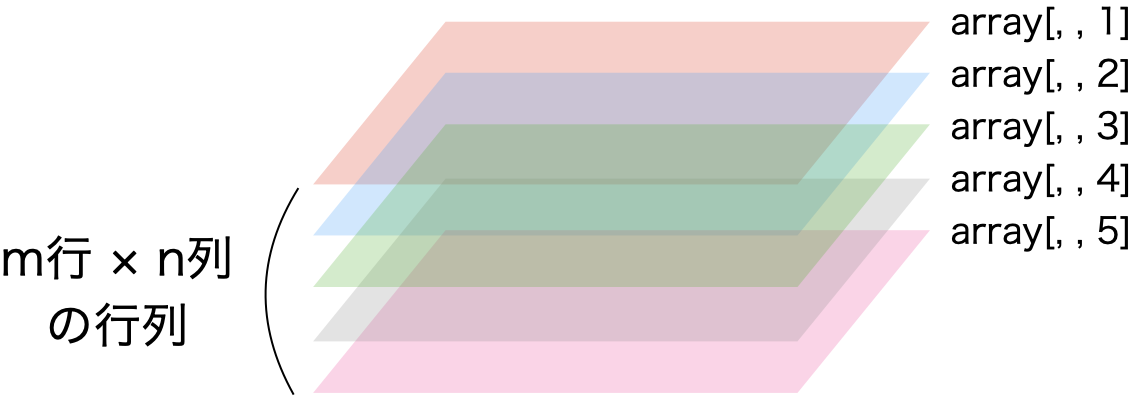
\includegraphics[width=0.75\textwidth,height=\textheight]{./Figs/DataStructure/array.png}

}

\caption{\label{fig-structure_array}配列型データのイメージ}

\end{figure}

したがって、配列型は行と列以外にも、層の要素も持つことになります。複数の行列で構成されている点では、リスト型と類似していますが、配列型は\textbf{同じサイズ}の\textbf{行列}のみで構成されている点が特徴です。

配列型は普段、扱う機会があまりありませんが、マルコフ連鎖モンテカルロ法
(MCMC)でベイジアン推定を行った後の事後分布データは配列型で格納される場合があります。

\hypertarget{ux914dux5217ux578bux30c7ux30fcux30bfux306eux4f5cux6210}{%
\subsection{配列型データの作成}\label{ux914dux5217ux578bux30c7ux30fcux30bfux306eux4f5cux6210}}

各行列は3行4列とし、4層構造とします。まずは、同じサイズの行列を作成し、それぞれ\texttt{Mat1}、\texttt{Mat2}、\texttt{Mat3}、\texttt{Mat4}と名付けます。

\begin{Shaded}
\begin{Highlighting}[numbers=left,,]
\NormalTok{Mat1 }\OtherTok{\textless{}{-}} \FunctionTok{matrix}\NormalTok{(}\FunctionTok{sample}\NormalTok{(}\DecValTok{1}\SpecialCharTok{:}\DecValTok{12}\NormalTok{, }\DecValTok{12}\NormalTok{, }\AttributeTok{replace =} \ConstantTok{TRUE}\NormalTok{), }\AttributeTok{byrow =} \ConstantTok{TRUE}\NormalTok{, }\AttributeTok{nrow =} \DecValTok{3}\NormalTok{)}
\NormalTok{Mat2 }\OtherTok{\textless{}{-}} \FunctionTok{matrix}\NormalTok{(}\FunctionTok{sample}\NormalTok{(}\DecValTok{1}\SpecialCharTok{:}\DecValTok{12}\NormalTok{, }\DecValTok{12}\NormalTok{, }\AttributeTok{replace =} \ConstantTok{TRUE}\NormalTok{), }\AttributeTok{byrow =} \ConstantTok{TRUE}\NormalTok{, }\AttributeTok{nrow =} \DecValTok{3}\NormalTok{)}
\NormalTok{Mat3 }\OtherTok{\textless{}{-}} \FunctionTok{matrix}\NormalTok{(}\FunctionTok{sample}\NormalTok{(}\DecValTok{1}\SpecialCharTok{:}\DecValTok{12}\NormalTok{, }\DecValTok{12}\NormalTok{, }\AttributeTok{replace =} \ConstantTok{TRUE}\NormalTok{), }\AttributeTok{byrow =} \ConstantTok{TRUE}\NormalTok{, }\AttributeTok{nrow =} \DecValTok{3}\NormalTok{)}
\NormalTok{Mat4 }\OtherTok{\textless{}{-}} \FunctionTok{matrix}\NormalTok{(}\FunctionTok{sample}\NormalTok{(}\DecValTok{1}\SpecialCharTok{:}\DecValTok{12}\NormalTok{, }\DecValTok{12}\NormalTok{, }\AttributeTok{replace =} \ConstantTok{TRUE}\NormalTok{), }\AttributeTok{byrow =} \ConstantTok{TRUE}\NormalTok{, }\AttributeTok{nrow =} \DecValTok{3}\NormalTok{)}
\end{Highlighting}
\end{Shaded}

\texttt{sample()}関数は初めてですね。これは与えられたベクトルの要素から無作為に要素を抽出する関数です。\texttt{sample(1:12,\ n)}なら\texttt{c(1,\ 2,\ 3,\ 4,\ 5,\ 6,\ 7,\ 8,\ 9,\ 10,\ 11,1\ 2)}から無作為に\texttt{n}個の要素を抽出するという意味です。\texttt{replace\ =\ TRUE}を指定すると、反復抽出、つまり、一回抽出された要素であっても抽出される可能性があることを意味します。デフォルトは\texttt{FALSE}ですが、この場合、一旦抽出された要素は二度と抽出されません。それではそれぞれの行列の中身を見てみましょう。

\begin{Shaded}
\begin{Highlighting}[numbers=left,,]
\NormalTok{Mat1}
\end{Highlighting}
\end{Shaded}

\begin{verbatim}
     [,1] [,2] [,3] [,4]
[1,]   10   11    4    2
[2,]    5    1    8    9
[3,]    2    1    9    4
\end{verbatim}

\begin{Shaded}
\begin{Highlighting}[numbers=left,,]
\NormalTok{Mat2}
\end{Highlighting}
\end{Shaded}

\begin{verbatim}
     [,1] [,2] [,3] [,4]
[1,]    3   12    4   11
[2,]    2    9    9    6
[3,]   10   10    8   11
\end{verbatim}

\begin{Shaded}
\begin{Highlighting}[numbers=left,,]
\NormalTok{Mat3}
\end{Highlighting}
\end{Shaded}

\begin{verbatim}
     [,1] [,2] [,3] [,4]
[1,]    4   12    2    2
[2,]    4    8   12   12
[3,]    7    4    9    2
\end{verbatim}

\begin{Shaded}
\begin{Highlighting}[numbers=left,,]
\NormalTok{Mat4}
\end{Highlighting}
\end{Shaded}

\begin{verbatim}
     [,1] [,2] [,3] [,4]
[1,]    8    6    6   12
[2,]    6    8    6    5
[3,]   10    4    3   12
\end{verbatim}

配列型データを作成するには\texttt{array()}関数を使います。引数としては行列名を\texttt{c()}で繋ぎ\footnote{元々はベクトルを入力しますが、行列を\texttt{c()}で繋ぐと自動的にベクトルに変換されます。}、\texttt{dim\ =}でarrayの大きさを指定するだけです。配列を作成した後はそのデータ構造も確認してみましょう。

\begin{Shaded}
\begin{Highlighting}[numbers=left,,]
\NormalTok{Array1 }\OtherTok{\textless{}{-}} \FunctionTok{array}\NormalTok{(}\FunctionTok{c}\NormalTok{(Mat1, Mat2, Mat3, Mat4), }\AttributeTok{dim =} \FunctionTok{c}\NormalTok{(}\DecValTok{3}\NormalTok{, }\DecValTok{4}\NormalTok{, }\DecValTok{4}\NormalTok{))}
\FunctionTok{class}\NormalTok{(Array1)}
\end{Highlighting}
\end{Shaded}

\begin{verbatim}
[1] "array"
\end{verbatim}

\texttt{dim\ =\ c(m,\ n,\ z)}の部分ですが、これは「\texttt{m}行\texttt{n}列の行列が\texttt{z}枚重ねる」という意味です。今回は3行4列の行列を4枚重ねるので\texttt{dim\ =\ c(3,\ 4,\ 4)}です。それでは\texttt{Array1}の中身を見てみます。

\begin{Shaded}
\begin{Highlighting}[numbers=left,,]
\NormalTok{Array1}
\end{Highlighting}
\end{Shaded}

\begin{verbatim}
, , 1

     [,1] [,2] [,3] [,4]
[1,]   10   11    4    2
[2,]    5    1    8    9
[3,]    2    1    9    4

, , 2

     [,1] [,2] [,3] [,4]
[1,]    3   12    4   11
[2,]    2    9    9    6
[3,]   10   10    8   11

, , 3

     [,1] [,2] [,3] [,4]
[1,]    4   12    2    2
[2,]    4    8   12   12
[3,]    7    4    9    2

, , 4

     [,1] [,2] [,3] [,4]
[1,]    8    6    6   12
[2,]    6    8    6    5
[3,]   10    4    3   12
\end{verbatim}

このように一つのオブジェクト内に複数の行列が格納されたオブジェクトが生成されます。

\hypertarget{ux914dux5217ux578bux30c7ux30fcux30bfux306eux64cdux4f5c}{%
\subsection{配列型データの操作}\label{ux914dux5217ux578bux30c7ux30fcux30bfux306eux64cdux4f5c}}

配列型データの操作は行列型に似ていますが、層というもう一つの次元があるため、\texttt{行列名{[}行番号,\ 列番号{]}}ではなく、\texttt{配列名{[}行番号,\ 列番号,\ 層番号{]}}を使います。たとえば、\texttt{Array1}の3番目の行列を抽出したい場合、\texttt{Array1{[},\ ,\ 3{]}}と入力します。

\begin{Shaded}
\begin{Highlighting}[numbers=left,,]
\NormalTok{Array1[, , }\DecValTok{3}\NormalTok{]}
\end{Highlighting}
\end{Shaded}

\begin{verbatim}
     [,1] [,2] [,3] [,4]
[1,]    4   12    2    2
[2,]    4    8   12   12
[3,]    7    4    9    2
\end{verbatim}

また、2番目の行列の3行目・1列目の要素を抽出するなら\texttt{Array1{[}3,\ 1,\ 2{]}}と入力します。

\begin{Shaded}
\begin{Highlighting}[numbers=left,,]
\NormalTok{Array1[}\DecValTok{3}\NormalTok{, }\DecValTok{1}\NormalTok{, }\DecValTok{2}\NormalTok{]}
\end{Highlighting}
\end{Shaded}

\begin{verbatim}
[1] 10
\end{verbatim}

配列型における操作の特徴の一つは全ての行列が同じ大きさを持つため、層を貫通した操作ができるという点です。たとえば、全ての層の2行目を抽出するなら、層番号を指定せず、行番号のみで抽出します。

\begin{Shaded}
\begin{Highlighting}[numbers=left,,]
\NormalTok{Array1[}\DecValTok{2}\NormalTok{, , ]}
\end{Highlighting}
\end{Shaded}

\begin{verbatim}
     [,1] [,2] [,3] [,4]
[1,]    5    2    4    6
[2,]    1    9    8    8
[3,]    8    9   12    6
[4,]    9    6   12    5
\end{verbatim}

ただ、返された結果は配列型でなく行列型であることに注意しましょう。たとえば、1番目の行列の2行目の要素は5,
1, 8,
9ですが、これは先ほど抽出された行列の1列目に該当します。また、2番目の行列の2行目の要素は2,
9, 9,
6であり、これは先ほどの抽出された行列の2列目となります。全層において特定の一列を抽出しても同じです。これは各層において抽出されたデータが行列でなく、ベクトルだからです。

一方、\textbf{複数}の行または列を抽出した場合、結果は配列型です。\texttt{Array1}の各層から1・2行目と1・2列目の要素、つまり大きさが2
\(\times\) 2の行列を抽出してみましょう。

\begin{Shaded}
\begin{Highlighting}[numbers=left,,]
\NormalTok{Array1[}\DecValTok{1}\SpecialCharTok{:}\DecValTok{2}\NormalTok{, }\DecValTok{1}\SpecialCharTok{:}\DecValTok{2}\NormalTok{, ]}
\end{Highlighting}
\end{Shaded}

\begin{verbatim}
, , 1

     [,1] [,2]
[1,]   10   11
[2,]    5    1

, , 2

     [,1] [,2]
[1,]    3   12
[2,]    2    9

, , 3

     [,1] [,2]
[1,]    4   12
[2,]    4    8

, , 4

     [,1] [,2]
[1,]    8    6
[2,]    6    8
\end{verbatim}

このように各層において抽出されたデータが行列だからです。自分の操作から得られた結果がどのようなデータ型・データ構造かを予め知っておくことで分析の効率が上がるでしょう。

\textbf{行列に名前を付けたい}

今回は各行列に1, 2, 3,
4という番号のみ割り当てましたが、実は行列に名前を付けることも可能です。そのためには配列データ作成時、\texttt{dimnames\ =}引数を指定する必要があります。

\begin{Shaded}
\begin{Highlighting}[numbers=left,,]
\NormalTok{Array2 }\OtherTok{\textless{}{-}} \FunctionTok{array}\NormalTok{(}\FunctionTok{c}\NormalTok{(Mat1, Mat2, Mat3, Mat4), }\AttributeTok{dim =} \FunctionTok{c}\NormalTok{(}\DecValTok{3}\NormalTok{, }\DecValTok{4}\NormalTok{, }\DecValTok{4}\NormalTok{),}
                \AttributeTok{dimnames =} \FunctionTok{list}\NormalTok{(}\ConstantTok{NULL}\NormalTok{, }
                                \ConstantTok{NULL}\NormalTok{, }
                                \FunctionTok{c}\NormalTok{(}\StringTok{"M1"}\NormalTok{, }\StringTok{"M2"}\NormalTok{, }\StringTok{"M3"}\NormalTok{, }\StringTok{"M4"}\NormalTok{))}
\NormalTok{                )}
\end{Highlighting}
\end{Shaded}

\texttt{dimnames\ =}引数は必ず長さ3のリスト型である必要があります。1番目と2番目の要素は行名と列名ですが、行列において一般的に使われないため、ここでは\texttt{NULL}にし、3番目の要素、つまり各層の名前だけを指定します。ここではそれぞれの層を\texttt{M1}、\texttt{M2}、\texttt{M3}、\texttt{M4}と名付けました。ここで\texttt{M4}のみを抽出する場合は、以下のように操作します。

\begin{Shaded}
\begin{Highlighting}[numbers=left,,]
\NormalTok{Array2[, , }\StringTok{"M4"}\NormalTok{]}
\end{Highlighting}
\end{Shaded}

\begin{verbatim}
     [,1] [,2] [,3] [,4]
[1,]    8    6    6   12
[2,]    6    8    6    5
[3,]   10    4    3   12
\end{verbatim}

むろん、これまでと同様、番号で抽出することも可能です。

\begin{Shaded}
\begin{Highlighting}[numbers=left,,]
\NormalTok{Array2[, , }\DecValTok{4}\NormalTok{]}
\end{Highlighting}
\end{Shaded}

\begin{verbatim}
     [,1] [,2] [,3] [,4]
[1,]    8    6    6   12
[2,]    6    8    6    5
[3,]   10    4    3   12
\end{verbatim}

\hypertarget{sec-programming}{%
\chapter{Rプログラミングの基礎}\label{sec-programming}}

 この章では統計ソフトウェアではなく、プログラミング言語としてのRについて解説する。プログラミングは難しいというイメージがあるかもしれないが、実は難しい。しかし、プログラミングをする場合にまず覚えるべき重要概念は、

\begin{enumerate}
\def\labelenumi{\arabic{enumi}.}
\tightlist
\item
  データの読み書き\footnote{具体的にはメモリの特定箇所にデータを書き込んだり、それを読み取んだりすること。}
\item
  条件分岐
\item
  反復
\end{enumerate}

の3つだけだ\footnote{チューリング完全 (Turing-complete)
  な言語の条件に「反復」はない。条件分岐でループを実行することができるからだ。よって、プログラミングを構成するのは「データの読み書き」と「条件分岐」のみとも考えられる。}。この3つだけでほとんどのプログラムが作れる。ただ、この単純さがプログラミングの難しさもあるとも言える。

 たとえば、ある数字の列を小さい順(昇順)に並び替えることを考えよう。\texttt{c(6,\ 3,\ 7,\ 2,\ 5,\ 1,\ 8,\ 4)}
という数列が与えられたとき、人間ならあまり苦労することなく、\texttt{c(1,\ 2,\ 3,\ 4,\ 5,\ 6,\ 7,\ 8)}
に並び替えられるだろう。しかし、その手順を「代入」、「条件分岐」、「反復」のみで明確に表現できるだろうか\footnote{並べ替え(ソート)アルゴリズムはプログラミングを学習する際に定番の題材であり、様々なアルゴリズムがある。}。もちろん、できる。よって、並べ替えはプログラミングによって実現することができる。Rには、数字を並べ替えるための\texttt{sort()}関数や\texttt{order()}関数などが用意されており、それらの組込関数を使えば良いのだが、組込関数は「代入」、「条件分岐」、「反復」を組み合わせて作られたものだ。

「代入」、「条件分岐」、「反復」という3つの概念さえ理解すれば何でもできるるという意味で、プログラミングは簡単だ。しかし、この3つだけで解決しないといけないという意味で、プログラミングは難しい。頻繁に利用する機能については、ほとんどのプログラミング言語があらかじめ作られた関数
(built-in function, 組込関数)
を数多く提供しており、ユーザである私たちは組込関数を使うのが賢明である。それでも条件分岐や反復について勉強する必要があるのは、私たち一般ユーザにとってもこれが必要な場面が多いからである。たとえば、同じ分析をデータだけ変えながら複数回実行するために反復を利用する。反復をうまく使えば、コードの量を数十分の一に減らすことも可能である。また、特定の条件に応じてデータを分類するときは条件分岐を使う。条件分岐を使いこなせないと、CalcやExcelなどのスプレッドシートでデータを目でみながら値を入力するという苦行を強いられるが\footnote{苦行であるだけでなく、スプレッドシート上でデータを書き換えると、入力ミスをおかしやすいし、そのミスを後で見つけるのが非常に困難である。したがって、データをスプレッドシート上で編集するのは絶対にやめるべきである。}、条件分岐が使えればそのような作業は必要ない。数行のプログラミングをするだけで、ほんの数秒で分類が終わる。

\hypertarget{sec-programming_intro}{%
\section{R言語の基礎概念}\label{sec-programming_intro}}

\hypertarget{ux30aaux30d6ux30b8ux30a7ux30afux30c8}{%
\subsection{オブジェクト}\label{ux30aaux30d6ux30b8ux30a7ux30afux30c8}}

 これまで「オブジェクト」や「関数」などという概念を定義せずに使ってきたが、ここではR言語の構成する基本的な概念についてもう少し詳細に解説する。これらは、プログラミングをする上である程度は意識的に使う必要があるものである。

 まず、\textbf{オブジェクト (object)}
とはメモリに割り当てられた「何か」である。「何か」に該当するのは、ベクトル
(vector)、行列 (matrix)、データフレーム (data frame)、リスト
(list)、関数 (function)
などである。一般的に、オブジェクトにはそれぞれ固有の(つまり、他のオブジェクトと重複しない)名前が付いている。

 たとえば、1から5までの自然数の数列を

\begin{Shaded}
\begin{Highlighting}[numbers=left,,]
\NormalTok{my\_vec1 }\OtherTok{\textless{}{-}} \FunctionTok{c}\NormalTok{(}\DecValTok{1}\NormalTok{, }\DecValTok{2}\NormalTok{, }\DecValTok{3}\NormalTok{, }\DecValTok{4}\NormalTok{, }\DecValTok{5}\NormalTok{)  }\CommentTok{\# my\_vec1 \textless{}{-} 1:5  でも同じ}
\end{Highlighting}
\end{Shaded}

のように\texttt{my\_vec1}という名前のオブジェクトに格納する。オブジェクトに名前をつけてメモリに割り当てると、その後
\texttt{my\_vec1}
と入力するだけでそのオブジェクトの中身を読み込むことができるようになる。

 ここで、次のように
\texttt{my\_vec1}の要素を2倍にする操作を考えてみよう。

\begin{Shaded}
\begin{Highlighting}[numbers=left,,]
\NormalTok{my\_vec1 }\SpecialCharTok{*} \DecValTok{2}
\end{Highlighting}
\end{Shaded}

\begin{verbatim}
[1]  2  4  6  8 10
\end{verbatim}

\texttt{my\_vec1}は、先ほど定義したオブジェクトである。では\texttt{2}はどうだろうか。2はメモリに割り当てられていないので、オブジェクトではないのだろうか。実は、この数字
\texttt{2}
もオブジェクトである。計算する瞬間のみ\texttt{2}がメモリに割り当てられ、計算が終わったらメモリから消されると考えれば良い。「Rに存在するあらゆるものはオブジェクトである
(Everything that exists in R is an object)」
\citep{Chambers:2016}。\texttt{*}
のような演算子でさえもオブジェクトである。

\hypertarget{ux30afux30e9ux30b9}{%
\subsection{クラス}\label{ux30afux30e9ux30b9}}

 \textbf{クラス (class)}
とはオブジェクトを特徴づける属性である。既に何度か \texttt{class()}
関数を使ってデータ型やデータ構造を確認したが、\texttt{class()}関数でオブジェクトのクラスを確認することができる。先ほど、\texttt{my\_vec1}も\texttt{*}も\texttt{2}もオブジェクトであると説明した。これらがすべてオブジェクトであるということは、何らかのクラス属性を持っているというこである。また、\texttt{class()}関数そのものもオブジェクトなので、何らかのクラスをもつ。確認してみよう。

\begin{Shaded}
\begin{Highlighting}[numbers=left,,]
\FunctionTok{class}\NormalTok{(my\_vec1)}
\end{Highlighting}
\end{Shaded}

\begin{verbatim}
[1] "numeric"
\end{verbatim}

\begin{Shaded}
\begin{Highlighting}[numbers=left,,]
\FunctionTok{class}\NormalTok{(}\StringTok{\textasciigrave{}}\AttributeTok{*}\StringTok{\textasciigrave{}}\NormalTok{)}
\end{Highlighting}
\end{Shaded}

\begin{verbatim}
[1] "function"
\end{verbatim}

\begin{Shaded}
\begin{Highlighting}[numbers=left,,]
\FunctionTok{class}\NormalTok{(}\DecValTok{2}\NormalTok{)}
\end{Highlighting}
\end{Shaded}

\begin{verbatim}
[1] "numeric"
\end{verbatim}

\begin{Shaded}
\begin{Highlighting}[numbers=left,,]
\FunctionTok{class}\NormalTok{(class)}
\end{Highlighting}
\end{Shaded}

\begin{verbatim}
[1] "function"
\end{verbatim}

 統計分析をする際に、Rのクラスを意識することはあまりない。しかし、Rでパッケージを開発したり、複雑な関数を自作する場合、オブジェクト指向プログラミング
(Object-oriented Programming; OOP)
の考え方が重要で、オブジェクトのクラスを厳密に定義する必要がある\footnote{RはOOPを実装するためにS3クラスをデフォルトで採用しているが、これはオブジェクト指向プログラミング言語としては厳密性を欠くところがある。Rでは、S3の代わりにS4やR6などの現代的なOOPを実装することもできる。}。

 自分でパッケージを開発しないとしても、クラスの概念は知っておいたほうが良い。この後説明する関数には引数というものがあるが、引数には特定のクラスのオブジェクトしか指定できない。関数の使い方がわからないときには\texttt{?関数名}
でヘルプを表示するが、ヘルプには各引数に使うべきクラスが書かれている。クラスについて何も知らないと、ヘルプを読んでも意味がわからないかもしれない。

 たとえば、Rコンソール上で\texttt{?mean}を入力して実行すると、
図~\ref{fig-programming_help} のような \texttt{mean()}
関数のヘルプが表示される。ヘルプに示されているとおり、\texttt{mean()}関数に必要な引数は
\texttt{x}、\texttt{trim}、\texttt{na.rm}である。仮引数\texttt{x}の説明を読むと、\texttt{x}
の実引数にはnumeric または logical
のベクトルクラスが使えることが分かる。さらに、date、date-time、time
interval が使えることも教えてくれる。

\begin{figure}

{\centering 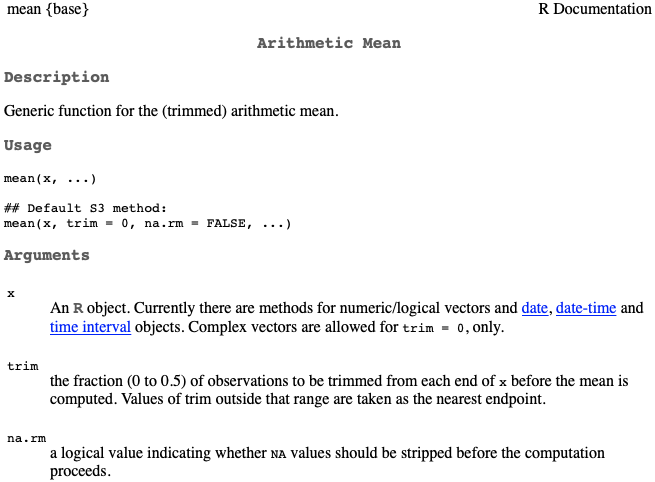
\includegraphics[width=0.75\textwidth,height=\textheight]{./Figs/Programming/help.png}

}

\caption{\label{fig-programming_help}\texttt{mean()}関数のヘルプ画面}

\end{figure}

 回帰分析を行う\texttt{lm()}関数の場合、\texttt{data}
という仮引数があるが、\texttt{data}の実引数に指定できるのは data.frame
クラスまたは
tibbleクラスのオブジェクトである\footnote{厳密には、tibble型データは3つのクラスを内部に有しており、その中にdata.frameが含まれる。}。通常はクラスを意識せずにRを使っても問題ないが、

\begin{enumerate}
\def\labelenumi{\arabic{enumi}.}
\tightlist
\item
  全てのオブジェクトにはクラスが付与されており、
\item
  関数 (の引数) ごとに実引数として使えるクラスが異なる
\end{enumerate}

という2点は覚えておこう。

\hypertarget{ux95a2ux6570ux3068ux5f15ux6570}{%
\subsection{関数と引数}\label{ux95a2ux6570ux3068ux5f15ux6570}}

 \textbf{関数 (function)}
は、入力されたデータを内部で決められた手順に従って処理し、その結果を返すものである。「Rで起こるあらゆることは関数の呼び出しである
(Everything that happens in R is a function
call)」\citep{Chambers:2016}。

 関数は \texttt{関数名(関数の入力となるオブジェクト)}
のように使う。たとえば、\texttt{class(my\_vec1)}は\texttt{my\_vec1}というオブジェクトのクラスを返す関数である。また、\texttt{sum(my\_vec1)}は\texttt{my\_vec1}の要素の総和を計算して返す関数である。

 関数は自分で作成することもできる(次章で説明する)。複雑な作業を繰り返す場合、その作業を関数として記述することで、一行でその作業を再現することが可能になる。「2度以上同じことを繰り返すなら関数を作れ」というのが、Rユーザの心得である。

 関数を使うためには、 \textbf{引数 (ひきすう)}
と呼ばれるものが必要である。例えば、\texttt{sum()}
関数はこれだけだと何もできない。何らかのオブジェクトがが入力として与えられないと、結果を返すことができない。\texttt{sum(my\_vec1)}のようにすることではじめて結果が返される。ここで\texttt{my\_vec1}が\texttt{sum()}関数の引数である。

 関数は引数は複数持つことができる。たとえば、欠測値を含む以下の\texttt{my\_vec2}を考えてみよう。

\begin{Shaded}
\begin{Highlighting}[numbers=left,,]
\NormalTok{my\_vec2 }\OtherTok{\textless{}{-}} \FunctionTok{c}\NormalTok{(}\DecValTok{1}\NormalTok{, }\DecValTok{2}\NormalTok{, }\DecValTok{3}\NormalTok{, }\ConstantTok{NA}\NormalTok{, }\DecValTok{5}\NormalTok{)}
\end{Highlighting}
\end{Shaded}

 この数列の総和を \texttt{sum()}関数で求めようとすると、結果は欠測値
\texttt{NA} になる。

\begin{Shaded}
\begin{Highlighting}[numbers=left,,]
\FunctionTok{sum}\NormalTok{(my\_vec2)}
\end{Highlighting}
\end{Shaded}

\begin{verbatim}
[1] NA
\end{verbatim}

 これは\texttt{sum()}の基本仕様が「入力に欠測値が含まれている場合は欠測値を返す」ことになっているためである。入力されたデータのなかで欠測値を除いたものの総和を求めるために、\texttt{sum()}はもう1つの引数が用意されている。それが
\texttt{na.rm}
である。\texttt{na.rm\ =\ TRUE}を指定すると、欠測値を除外した総和を返す。

\begin{Shaded}
\begin{Highlighting}[numbers=left,,]
\FunctionTok{sum}\NormalTok{(my\_vec2, }\AttributeTok{na.rm =} \ConstantTok{TRUE}\NormalTok{)}
\end{Highlighting}
\end{Shaded}

\begin{verbatim}
[1] 11
\end{verbatim}

 第\ref{sec-rbasic}章で説明したとおり、\texttt{na.rm}
などのように引数を区別するために関数によって用意されたものを\textbf{仮引数
(parameter)} と呼び、\texttt{TRUE}
のように引数の中身としてユーザが指定するものを\textbf{実引数 (argument)}
と呼ぶ。\texttt{my\_vec2} は実引数である。

 引数を指定するとき、\texttt{my\_vec2}のように仮引数を明示しないこともある。多くの場合、それがなければ関数がそもそも動かないという第1引数の仮引数は明示しないことが多い。そもそも、第1引数には仮引数がない(名前がない)場合もある。\texttt{sum()}
関数の第1引数はnumeric または complex
型のベクトルだが、仮引数がそもそもない(\texttt{...}
で定義されている)。

 しかし、第1引数以外については、\texttt{na.rm\ =\ TRUE}
のように仮引数を明示すべきである。関数によっては数十個の引数をとるものもあり、仮引数を明示しないと、どの実引数がどの仮引数に対応するのかわかりにくい。

 多くの引数は関数によって定義された既定値 (default value)
をもっている。たとえば、\texttt{sum()}関数の \texttt{na.rm} の既定値は
\texttt{FALSE}
である。既定値が用意されている場合、その引数を指定せずに関数を使うことができる。

 ある関数がどのような引数を要求しているか、その既定値は何か、引数として何か決められたデータ型/データ構造があるかを調べたいときは
\texttt{?関数名} (\texttt{()}がないことに注意)または
\texttt{help(関数名)}をコンソールに入力する。多くの関数に詳細なヘルプが付いているので、ネットで検索したり、誰かに質問する前にひとまずヘルプを読むべきである。

\begin{center}\rule{0.5\linewidth}{0.5pt}\end{center}

\hypertarget{sec-programming_style}{%
\section{Rのコーディングスタイル}\label{sec-programming_style}}

 Rコードの書き方に唯一の正解はない。文法が正しければ、つまり、Rが意図どおりの実行結果を出してくれさえすれば、それは「正しい」コードである。しかし、コードというのは、一度書けば二度と読まないというものではない。最初に「書く」とき以外に、「修正する」ときや「再利用」するときなどに繰り返し読むことになる。また、共同研究をする場合には共同研究者がコードを読む。さらに、近年では研究成果を報告する際に分析に利用したコードを後悔公開することも当たり前になりつつあり、その場合には自分で書いたコードを世界中の人が読む可能性がある。

 ここで大事なのは、Rコードを読むのはRだけではないということである。人間も重要な「読者」である。Rコードを書くときは人間に優しいコードを書くように心がえよう。唯一の正解がなくても、読みやすく、多くの人が採用している標準的な書き方はある。ここでは、人間に優しいコードを書くためのコーディングスタイルについて説明しよう。

\hypertarget{ux30aaux30d6ux30b8ux30a7ux30afux30c8ux540d}{%
\subsection{オブジェクト名}\label{ux30aaux30d6ux30b8ux30a7ux30afux30c8ux540d}}

 ベクトル、データフレーム、自作の関数などのすべてのオブジェクトには名前をつける必要がある(ラムダ式などの無名関数を除く)。名前はある程度自由に付けることができるが、大事な原則がある。それは、

\begin{itemize}
\tightlist
\item
  \textbf{オブジェクト名は英数字と限られた記号のみにする}
\item
  \textbf{数字で始まる変数名は避ける}
\end{itemize}

1つ目は原則にすぎない。よって、日本語やハングルの変数名をつけることもできる。しかし、それは推奨しない。英数字以外(マルチバイト文字)は文字化けの可能性がある(文字コードの問題が発生する)し、コードを書く際列がずれる原因にもなる

\begin{Shaded}
\begin{Highlighting}[numbers=left,,]
\NormalTok{var1 }\OtherTok{\textless{}{-}} \FunctionTok{c}\NormalTok{(}\DecValTok{2}\NormalTok{, }\DecValTok{3}\NormalTok{, }\DecValTok{5}\NormalTok{, }\DecValTok{7}\NormalTok{, }\DecValTok{11}\NormalTok{)      }\CommentTok{\# 推奨}
\end{Highlighting}
\end{Shaded}

\begin{Shaded}
\begin{Highlighting}[numbers=left,,]
\NormalTok{変数1 }\OtherTok{\textless{}{-}} \FunctionTok{c}\NormalTok{(}\DecValTok{2}\NormalTok{, }\DecValTok{3}\NormalTok{, }\DecValTok{5}\NormalTok{, }\DecValTok{7}\NormalTok{, }\DecValTok{11}\NormalTok{)     }\CommentTok{\# 非推奨}
\end{Highlighting}
\end{Shaded}

\begin{Shaded}
\begin{Highlighting}[numbers=left,,]
\NormalTok{var1}
\end{Highlighting}
\end{Shaded}

\begin{verbatim}
[1]  2  3  5  7 11
\end{verbatim}

\begin{Shaded}
\begin{Highlighting}[numbers=left,,]
\NormalTok{変数1}
\end{Highlighting}
\end{Shaded}

\begin{verbatim}
[1]  2  3  5  7 11
\end{verbatim}

 2つ目のルールは必ず守る必要がある。つまり、数字で始まるオブジェクト名は作成できない。

\begin{Shaded}
\begin{Highlighting}[numbers=left,,]
\NormalTok{100A }\OtherTok{\textless{}{-}} \StringTok{"R"}
\end{Highlighting}
\end{Shaded}

\begin{verbatim}
Error: <text>:1:4: unexpected symbol
1: 100A
       ^
\end{verbatim}

\textbf{予約語を避ける}

 Rが提供する組込の関数やオブジェクトと重複する名前を自分で作成するオブジェクトに付けるのは避けよう。例えば、Rには円周率
(\(\pi\)) が\texttt{pi}という名前で用意されている。

\begin{Shaded}
\begin{Highlighting}[numbers=left,,]
\NormalTok{pi}
\end{Highlighting}
\end{Shaded}

\begin{verbatim}
[1] 3.141593
\end{verbatim}

\texttt{pi}という名前で新しい変数を作ることはできる。

\begin{Shaded}
\begin{Highlighting}[numbers=left,,]
\NormalTok{pi  }\OtherTok{\textless{}{-}} \DecValTok{777}
\end{Highlighting}
\end{Shaded}

しかし、既存の\texttt{pi}が上書きされてしまうので避けたほうが良い。

\begin{Shaded}
\begin{Highlighting}[numbers=left,,]
\NormalTok{pi   }\CommentTok{\# もはや円周率ではない}
\end{Highlighting}
\end{Shaded}

\begin{verbatim}
[1] 777
\end{verbatim}

元の円周率を使うこともできるが、手間が増える。

\begin{Shaded}
\begin{Highlighting}[numbers=left,,]
\NormalTok{base}\SpecialCharTok{::}\NormalTok{pi}
\end{Highlighting}
\end{Shaded}

\begin{verbatim}
[1] 3.141593
\end{verbatim}

 また、ユーザが自由に使えない名前もある。それらの名前を「予約語」と呼ぶ。予約語の使用は禁止されている。

\begin{Shaded}
\begin{Highlighting}[numbers=left,,]
\ControlFlowTok{if}  \OtherTok{\textless{}{-}} \StringTok{"YY"}
\end{Highlighting}
\end{Shaded}

\begin{verbatim}
Error: <text>:1:5: unexpected assignment
1: if  <-
        ^
\end{verbatim}

\begin{Shaded}
\begin{Highlighting}[numbers=left,,]
\ControlFlowTok{for} \OtherTok{\textless{}{-}} \StringTok{"JS"}
\end{Highlighting}
\end{Shaded}

\begin{verbatim}
Error: <text>:1:5: unexpected assignment
1: for <-
        ^
\end{verbatim}

\begin{Shaded}
\begin{Highlighting}[numbers=left,,]
\ConstantTok{TRUE} \OtherTok{\textless{}{-}} \StringTok{"いつもひとつ!"}
\end{Highlighting}
\end{Shaded}

\begin{verbatim}
Error in TRUE <- "いつもひとつ!": invalid (do_set) left-hand side to assignment
\end{verbatim}

このように、予約語はそもそも使えないので、それほど意識する必要はない。

 ただし、以下のコードのようなことが起こるので注意してほしい。

\begin{Shaded}
\begin{Highlighting}[numbers=left,,]
\NormalTok{vals }\OtherTok{\textless{}{-}} \DecValTok{1}\SpecialCharTok{:}\DecValTok{5}
\NormalTok{vals[}\FunctionTok{c}\NormalTok{(}\ConstantTok{TRUE}\NormalTok{, }\ConstantTok{TRUE}\NormalTok{, }\ConstantTok{FALSE}\NormalTok{, }\ConstantTok{FALSE}\NormalTok{, }\ConstantTok{TRUE}\NormalTok{)]}
\end{Highlighting}
\end{Shaded}

\begin{verbatim}
[1] 1 2 5
\end{verbatim}

\begin{Shaded}
\begin{Highlighting}[numbers=left,,]
\NormalTok{vals[}\FunctionTok{c}\NormalTok{(T, T, F, F, T)]}
\end{Highlighting}
\end{Shaded}

\begin{verbatim}
[1] 1 2 5
\end{verbatim}

ここから、\texttt{T} は \texttt{TRUE}、\texttt{F} は \texttt{FALSE}
と同じ働きをしていることがわかる。ここで、次のコードを実行してみよう。

\begin{Shaded}
\begin{Highlighting}[numbers=left,,]
\NormalTok{T }\OtherTok{\textless{}{-}} \StringTok{"Taylor"}
\NormalTok{F }\OtherTok{\textless{}{-}} \StringTok{"Fourier"}
\NormalTok{vals[}\FunctionTok{c}\NormalTok{(T, T, F, F, T)]}
\end{Highlighting}
\end{Shaded}

\begin{verbatim}
[1] NA NA NA NA NA
\end{verbatim}

このように、\texttt{T}
と\texttt{F}はあらかじめ使える状態で用意されているものの、予約語ではないので値が代入できてしまう。しかし、\texttt{T}
と\texttt{F}
を自分で定義したオブジェクトの名前に使うと混乱の元になるので、使用は避けるのが無難である。

 また、\texttt{TRUE} と \texttt{FALSE} を \texttt{T} や\texttt{F}
で済ませる悪習は廃して常に完全にスペルすべきである。

\textbf{「短さ」と「分かりやすさ」を重視する}

オブジェクト名を見るだけでその中にどのようなデータが含まれているか推測できる名前をつけるべきである。たとえば、性別を表す変数を作るなら、

\begin{Shaded}
\begin{Highlighting}[numbers=left,,]
\NormalTok{var2 }\OtherTok{\textless{}{-}} \FunctionTok{c}\NormalTok{(}\StringTok{"female"}\NormalTok{, }\StringTok{"male"}\NormalTok{, }\StringTok{"male"}\NormalTok{, }\StringTok{"female"}\NormalTok{)}
\end{Highlighting}
\end{Shaded}

ではなく、

\begin{Shaded}
\begin{Highlighting}[numbers=left,,]
\NormalTok{gender }\OtherTok{\textless{}{-}} \FunctionTok{c}\NormalTok{(}\StringTok{"female"}\NormalTok{, }\StringTok{"male"}\NormalTok{, }\StringTok{"male"}\NormalTok{, }\StringTok{"female"}\NormalTok{)}
\end{Highlighting}
\end{Shaded}

としたほうが良い。\texttt{gender}
という名前がついていれば、「この変数には性別に関する情報が入っているだろう」と容易に想像できる。

 また、オブジェクト名は、短くて読みやすいほうが良い。数学の成績データをもつ次のオブジェクトについて考えよう。

\begin{Shaded}
\begin{Highlighting}[numbers=left,,]
\NormalTok{mathematicsscore }\OtherTok{\textless{}{-}} \FunctionTok{c}\NormalTok{(}\DecValTok{30}\NormalTok{, }\DecValTok{91}\NormalTok{, }\DecValTok{43}\NormalTok{, }\DecValTok{77}\NormalTok{, }\DecValTok{100}\NormalTok{)}
\end{Highlighting}
\end{Shaded}

オブジェクト名から、中にどのような情報が含まれるか想像することはできる。しかし、この名前は長く、読みにくい。そこで、次のように名前を変えたほうが良い。

\begin{Shaded}
\begin{Highlighting}[numbers=left,,]
\NormalTok{MathScore  }\OtherTok{\textless{}{-}} \FunctionTok{c}\NormalTok{(}\DecValTok{30}\NormalTok{, }\DecValTok{91}\NormalTok{, }\DecValTok{43}\NormalTok{, }\DecValTok{77}\NormalTok{, }\DecValTok{100}\NormalTok{)}
\NormalTok{mathScore  }\OtherTok{\textless{}{-}} \FunctionTok{c}\NormalTok{(}\DecValTok{30}\NormalTok{, }\DecValTok{91}\NormalTok{, }\DecValTok{43}\NormalTok{, }\DecValTok{77}\NormalTok{, }\DecValTok{100}\NormalTok{)}
\NormalTok{math\_score }\OtherTok{\textless{}{-}} \FunctionTok{c}\NormalTok{(}\DecValTok{30}\NormalTok{, }\DecValTok{91}\NormalTok{, }\DecValTok{43}\NormalTok{, }\DecValTok{77}\NormalTok{, }\DecValTok{100}\NormalTok{)}
\end{Highlighting}
\end{Shaded}

これらの例では、mathematics を math
に縮め、\texttt{math}と\texttt{score}の間に区切りを入れて読みやすくしている。大文字と小文字の組み合わせで区切る方法は\textbf{キャメルケース
(camel
case)}と呼ばれ、大文字から始まるキャメルケースを\textbf{大文字キャメルケース
(upper camel
case)}、小文字から始まるキャメルケースを\textbf{小文字キャメルケース
(lower camel case)} と呼ぶ。また、\texttt{\_}(アンダーバー, アンスコ)
で区切る方法は\textbf{スネークケース (snake case)}
と呼ばれる。キャメルケースとスネークケースは、一貫した方法で使えばどちらを使っても良いだろう。

 かつては ``.''
を使って単語を繋ぐのが標準的だった時代もあり、組込関数には ``.''
を使ったものも多い。\texttt{data.frame()} や \texttt{read.csv()}
などがその例である。しかし、``.''
はクラスのメソッドとして使われることがあり、混乱するので使うのは避けたほうが良い。\{tidyverse\}
では、\texttt{readr::read\_csv()}
のように、スネークケースが採用されている。他にも
\texttt{-}(ハイフン)で区切る\textbf{チェーンケース (chain
case)}というのもあるが、Rで\texttt{-}は「マイナス(減算演算子)」であり、チェーンケースは使えない\footnote{チェーンケースは、COBOLやLISPのような言語では使われる。どうしても使いたければ、変数名全体をバックティック(\texttt{\textasciigrave{}})で囲んで\texttt{\textasciigrave{}math-score\textasciigrave{}\ \textless{}-\ 10}
  のようにする方法もあるが、もちろん推奨しない。}。

\hypertarget{ux6539ux884c}{%
\subsection{改行}\label{ux6539ux884c}}

 コードは1行が長すぎないように適宜改行する。Rやパッケージなどが提供している関数のなかには10個以上の引数を必要とするものもあり。コードを1行で書こうとするとコードの可読性が著しく低くなってしまう。

 1行に何文字入れるべきかについて決まったルールはないが、1行の最大文字数を半角80字にするという基準が伝統的に使われてきた。これま昔のパソコンで使ったパンチカード
( 図~\ref{fig-programming_punchcard}
)では1行に80個の穴を開けることができたことに由来する。

\begin{figure}

{\centering \includegraphics[width=0.75\textwidth,height=\textheight]{./Figs/Programming/Punchcard.png}

}

\caption{\label{fig-programming_punchcard}パンチカードの例}

\end{figure}

最近は昔と比べてモニタのサイズが大きく、解像度も高いので、80文字にこだわる必要はない。自分のRStudioのSource
Paneに収まるよう、切りがいいところで改行しよう。

\hypertarget{ux30b9ux30daux30fcux30b9ux3068ux30a4ux30f3ux30c7ux30f3ux30c8}{%
\subsection{スペースとインデント}\label{ux30b9ux30daux30fcux30b9ux3068ux30a4ux30f3ux30c7ux30f3ux30c8}}

 適切なスペースはコードの可読性を向上させる。以下の2つのコードは同じ内容を実行するが、後者にはスペースがないので読にくい。

\begin{Shaded}
\begin{Highlighting}[numbers=left,,]
\CommentTok{\# 良い例}
\FunctionTok{sum}\NormalTok{(my\_vec2, }\AttributeTok{na.rm =} \ConstantTok{TRUE}\NormalTok{)}

\CommentTok{\# 悪い例}
\FunctionTok{sum}\NormalTok{(my\_vec2,}\AttributeTok{na.rm=}\ConstantTok{TRUE}\NormalTok{)}
\end{Highlighting}
\end{Shaded}

 どこにスペースを入れるかについてのルールは特になり。Rは「\textbf{半角}スペース」を無視するので、プログラムの動作に関して言えば、\textbf{半角}スペースはあってもなくても同じである。標準的なルールとして、「\texttt{,}の後にスペース」、「演算子の前後にスペース」などが考えらえる。ただし、\texttt{\^{}}の前後にはスペースを入れないことが多い。また、後ほど紹介する\texttt{for()\{\}}、\texttt{while()\{\}}、\texttt{if()\{\}}などのように、関数以外の
\texttt{()}の前後にはスペースを入れる。それに対し、\texttt{sum()} や
\texttt{read.csv()}
などのように、関数のかっこの場合には、関数名と\texttt{()}の間にスペースを入れない。

 また、スペースを2回以上入れることもある。たとえば、あるデータフレームを作る例を考えよう。

\begin{Shaded}
\begin{Highlighting}[numbers=left,,]
\CommentTok{\# 良い例}
\FunctionTok{data.frame}\NormalTok{(}
  \AttributeTok{name     =} \FunctionTok{c}\NormalTok{(}\StringTok{"Song"}\NormalTok{,  }\StringTok{"Yanai"}\NormalTok{, }\StringTok{"Wickham"}\NormalTok{),}
  \AttributeTok{favorite =} \FunctionTok{c}\NormalTok{(}\StringTok{"Ramen"}\NormalTok{, }\StringTok{"Cat"}\NormalTok{,   }\StringTok{"R"}\NormalTok{),}
  \AttributeTok{gender   =} \FunctionTok{c}\NormalTok{(}\StringTok{"Male"}\NormalTok{,  }\StringTok{"Male"}\NormalTok{,  }\StringTok{"Male"}\NormalTok{)}
\NormalTok{)}

\CommentTok{\# 悪い例}
\FunctionTok{data.frame}\NormalTok{(}
  \AttributeTok{name =} \FunctionTok{c}\NormalTok{(}\StringTok{"Song"}\NormalTok{, }\StringTok{"Yanai"}\NormalTok{, }\StringTok{"Hadley"}\NormalTok{),}
  \AttributeTok{favorite =} \FunctionTok{c}\NormalTok{(}\StringTok{"Ramen"}\NormalTok{, }\StringTok{"Cat"}\NormalTok{, }\StringTok{"R"}\NormalTok{),}
  \AttributeTok{gender =} \FunctionTok{c}\NormalTok{(}\StringTok{"Male"}\NormalTok{, }\StringTok{"Male"}\NormalTok{, }\StringTok{"Male"}\NormalTok{)}
\NormalTok{)}
\end{Highlighting}
\end{Shaded}

上の2つのコードの内容は同じだが、前者のほうが読みやすい。

 ここでもう1つ注目してほしいのは、「字下げ
(indent)」の使い方である。上のコードは次のように一行にまとめることができるが、読みにくい。

\begin{Shaded}
\begin{Highlighting}[numbers=left,,]
\CommentTok{\# 邪悪な例}
\FunctionTok{data.frame}\NormalTok{(}\AttributeTok{name=}\FunctionTok{c}\NormalTok{(}\StringTok{"Song"}\NormalTok{,}\StringTok{"Yanai"}\NormalTok{,}\StringTok{"Hadley"}\NormalTok{),}\AttributeTok{favorite=}\FunctionTok{c}\NormalTok{(}\StringTok{"Ramen"}\NormalTok{,}\StringTok{"Cat"}\NormalTok{,}\StringTok{"R"}\NormalTok{),}\AttributeTok{fender=}\FunctionTok{c}\NormalTok{(}\StringTok{"Male"}\NormalTok{,}\StringTok{"Male"}\NormalTok{,}\StringTok{"Male"}\NormalTok{))}
\end{Highlighting}
\end{Shaded}

このように1行のコードが長い場合、「改行」が重要である。しかし、Rの最も基本的なルールは「1行に1つのコード」なので、改行するとこのルールを破ることになってしまう。そこで、コードの途中で改行するときは、2行目以降を字下げすることで、1つのコードが前の行から続いていることを明確にしよう。前の行の続きの行は2文字(または4文字)分字下げする。こうすることで、「この行は上の行の続き」ということが「見て」わかるようになる。

\begin{Shaded}
\begin{Highlighting}[numbers=left,,]
\CommentTok{\# 良い例}
\FunctionTok{data.frame}\NormalTok{(}
  \AttributeTok{name     =} \FunctionTok{c}\NormalTok{(}\StringTok{"Song"}\NormalTok{,  }\StringTok{"Yanai"}\NormalTok{, }\StringTok{"Hadley"}\NormalTok{),}
  \AttributeTok{favorite =} \FunctionTok{c}\NormalTok{(}\StringTok{"Ramen"}\NormalTok{, }\StringTok{"Cat"}\NormalTok{,   }\StringTok{"R"}\NormalTok{),}
  \AttributeTok{gender   =} \FunctionTok{c}\NormalTok{(}\StringTok{"Male"}\NormalTok{,  }\StringTok{"Male"}\NormalTok{,  }\StringTok{"Male"}\NormalTok{)}
\NormalTok{)}

\CommentTok{\# 悪い例}
\FunctionTok{data.frame}\NormalTok{(}
\AttributeTok{name     =} \FunctionTok{c}\NormalTok{(}\StringTok{"Song"}\NormalTok{,  }\StringTok{"Yanai"}\NormalTok{, }\StringTok{"Hadley"}\NormalTok{),}
\AttributeTok{favorite =} \FunctionTok{c}\NormalTok{(}\StringTok{"Ramen"}\NormalTok{, }\StringTok{"Cat"}\NormalTok{,   }\StringTok{"R"}\NormalTok{),}
\AttributeTok{gender   =} \FunctionTok{c}\NormalTok{(}\StringTok{"Male"}\NormalTok{,  }\StringTok{"Male"}\NormalTok{,  }\StringTok{"Male"}\NormalTok{)}
\NormalTok{)}
\end{Highlighting}
\end{Shaded}

 RStudioは自動的に字下げをしてくれるので、RStudioを使っているならあまり意識する必要はない。自動で字下げしてくれないエディタを使っている場合は、字下げに気をつけよう。

\hypertarget{ux4ee3ux5165}{%
\subsection{代入}\label{ux4ee3ux5165}}

オブジェクトに値を代入する演算子として、これまで \texttt{\textless{}-}
を使ってきたが、\texttt{=}を使うこともできる。R以外の多くのプログラミング言語では、代入演算子として\texttt{=}を採用している。しかし、引数の指定と代入を区別するためん、本書では\texttt{\textless{}-}の使用を推奨する。また、既に説明したとおり、option
+ \texttt{-}(macOSの場合)または Alt + \texttt{-}(Windows
の場合)というショートカットを使うと、\texttt{\textless{}-}
だけでなく、その前後のスペースを自動的に挿入してくれる。コードが読みやすくなるので、代入演算子は常にショートカットで入力する習慣をつけよう。

 この節で説明したコードの書き方は、コーディングスタイルの一部に過ぎない。本書では、できるだけ読みやすいコードを例として示すことを心がけている。最初は本書(あるいは他の本やウェブサイトに掲載されているもののなかで気に入ったもの)のスタイルを真似して書いてみてほしい。コードを書き写しているうちに、自にとって最善の書き方が見えてくるだろう。

 コーディングスタイルについては、以下の2つの資料がさらに詳しい。とりわけ、羽鳥先生が書いた\href{https://style.tidyverse.org}{The
tidyverse style guide}
は事実上の業界標準であり、\href{https://google.github.io/styleguide/Rguide.html}{Google's
Style Guide} も
このガイドをベースにしている。かなりの分量だが、パッケージ開発などを考えているなら一度は目を通しておいたほうが良いだろう。

\begin{itemize}
\tightlist
\item
  \href{https://style.tidyverse.org}{The tidyverse style guide}
\item
  \href{https://google.github.io/styleguide/Rguide.html}{Google's Style
  Guide}
\end{itemize}

\begin{center}\rule{0.5\linewidth}{0.5pt}\end{center}

\hypertarget{sec-programming_iteration}{%
\section{反復}\label{sec-programming_iteration}}

 人間があまり得意ではないが、コンピュータが得意とする代表的な作業が「反復作業」である。普通の人間なら数時間から数年かかるような退屈な反復作業でも、コンピュータを使えば数秒で終わることが多い。Rでもさまざまな反復作業を行うことができる。

 反復作業を行うときは、反復作業を「いつ終わらせるか」を考えなくてはならない。終わりを規程する方法として、以下の2つが考えられる。

\begin{enumerate}
\def\labelenumi{\arabic{enumi}.}
\tightlist
\item
  処理を繰り返し回数を指定し、その回数に達したら終了する: \texttt{for}
  文を使う
\item
  一定の条件を指定し、その条件が満たされるときに処理を終了する:
  \texttt{while} 文を使う
\end{enumerate}

この節では、これら2つのケースのそれぞれについて解説する。

\hypertarget{for-ux306bux3088ux308bux53cdux5fa9}{%
\subsection{\texorpdfstring{\texttt{for}
による反復}{for による反復}}\label{for-ux306bux3088ux308bux53cdux5fa9}}

 \texttt{for}を利用した反復を、\textbf{forループ}
と呼ぶ。まず、forループの雛形をみてみよう。

\begin{Shaded}
\begin{Highlighting}[]
\ControlFlowTok{for}\NormalTok{ (任意の変数 }\ControlFlowTok{in}\NormalTok{ ベクトル) \{}
\NormalTok{  処理内容}
\NormalTok{\}}
\end{Highlighting}
\end{Shaded}

任意の変数の選び方はいろいろ考えられるが、よく使うのはインデクス (index)
\texttt{i}
である。このインデクスはforループの内部で使うために用いられる変数である。そして、\texttt{in}
の後の「ベクトル」には長さ1以上のベクトルを指定する。ベクトルは必ずしもnumeric型である必要はないが、インデクスを利用したforループではインデクスを指定する正の整数を要素にもつベクトルを使う。

 また、\texttt{\{\}}内の内容が1行のみの場合には、\texttt{\{\}}は省略しても良い。その場合、処理内容を\texttt{()}の直後に書。つまり、以下のような書き方もできる。

\begin{Shaded}
\begin{Highlighting}[]
\ControlFlowTok{for}\NormalTok{ (任意の変数 }\ControlFlowTok{in}\NormalTok{ ベクトル) 処理内容}
\end{Highlighting}
\end{Shaded}

これは\texttt{for}だけでなく、\texttt{if}や\texttt{function()}など、\texttt{\{\}}で処理内容を囲む関数に共通である。処理内容が2行以上の場合は、必ず\texttt{\{\}}で囲むようにしよう。

 例として、インデクス \(i\)
の内容を画面に表示することを\texttt{N}回繰り返すforループを書いてみよう。繰り返し回数を指定するために、\texttt{for\ (i\ in\ 1:N)}と書く。5回繰り返すなら\texttt{for\ (i\ in\ 1:5)}とする。\texttt{1:5}は\texttt{c(1,\ 2,\ 3,\ 4,\ 5)}と同じなので、\texttt{for\ (i\ in\ c(1,\ 2,\ 3,\ 4,\ 5))}でもいいが、\texttt{1:5}
を使って書いたほうが、コードが読みやすい。

 以下コードを作成し、実行してみよう。このコードは3行がひとつのかたまりになったコードである。\texttt{for}の行(あるいは最後の\texttt{\}}の行)にカーソルを置いた状態で
Cmd/Ctrl + Return/Enter を押せば、forループ全体が一挙に実行される。

\begin{Shaded}
\begin{Highlighting}[numbers=left,,]
\CommentTok{\# 以下のコードはこのように書くことも可能}
\CommentTok{\# for(i in 1:5) print(i)}
\ControlFlowTok{for}\NormalTok{ (i }\ControlFlowTok{in} \DecValTok{1}\SpecialCharTok{:}\DecValTok{5}\NormalTok{) \{}
  \FunctionTok{print}\NormalTok{(i)}
\NormalTok{\}}
\end{Highlighting}
\end{Shaded}

\begin{verbatim}
[1] 1
[1] 2
[1] 3
[1] 4
[1] 5
\end{verbatim}

1から5までの数字が表示された。

 ここで、このforループがどのような順番で処理を実行したのか確認してみよう。上のコードは、次のようなステップを踏んで1から5までの数字を画面に表示している。

\begin{enumerate}
\def\labelenumi{\arabic{enumi}.}
\tightlist
\item
  \texttt{i}にベクトル\texttt{1:5}の最初の要素を代入
  (\texttt{i\ \textless{}-\ 1})
\item
  \texttt{print(i)}を実行
\item
  \texttt{\{\}}中身の処理が終わったら\texttt{i}にベクトル\texttt{1:5}内の次の要素を代入
  (\texttt{i\ \textless{}-\ 2})
\item
  \texttt{print(i)}を実行
\item
  \texttt{\{\}}中身の処理が終わったら\texttt{i}にベクトル\texttt{1:5}内の次の要素を代入
  (\texttt{i\ \textless{}-\ 3})
\item
  \texttt{print(i)}を実行
\item
  \texttt{\{\}}中身の処理が終わったら\texttt{i}にベクトル\texttt{1:5}内の次の要素を代入
  (\texttt{i\ \textless{}-\ 4})
\item
  \texttt{print(i)}を実行
\item
  \texttt{\{\}}中身の処理が終わったら\texttt{i}にベクトル\texttt{1:5}内の次の要素を代入
  (\texttt{i\ \textless{}-\ 5})
\item
  \texttt{print(i)}を実行
\item
  \texttt{\{\}}中身の処理が終わったら\texttt{i}にベクトル\texttt{1:5}内の次の要素を代入するが、\texttt{5}が最後の要素なので反復終了
\end{enumerate}

この手順を要約すると、次のようになる。

\begin{itemize}
\tightlist
\item
  任意の変数 (ここでは\texttt{i})にベクトル
  (ここでは\texttt{1:5})の最初の要素が格納され、\texttt{\{\}}内の処理を行う。
\item
  \texttt{\{\}}内の処理が終わったら、ベクトル
  (ここでは\texttt{1:5})の次の要素を任意の変数
  (ここでは\texttt{i})に格納し、\texttt{\{\}}内の処理を行う。
\item
  格納できる要素がなくなったら反復を終了する。

  \begin{itemize}
  \tightlist
  \item
    したがって、反復はベクトル
    (ここでは\texttt{1:5})の長さだけ実行される (ここでは5回)。
  \end{itemize}
\end{itemize}

 反復回数はベクトルの長さで決まる。既に述べたとおり、\texttt{1:5}のような書き方でなく、普通のベクトルを指定しても問題ない。たとえば、長さ6の
\texttt{dmg\_vals}
というベクトルを作り、その要素を出力するコードを書いてみよう。

\begin{Shaded}
\begin{Highlighting}[numbers=left,,]
\NormalTok{dmg\_vals }\OtherTok{\textless{}{-}} \FunctionTok{c}\NormalTok{(}\DecValTok{24}\NormalTok{, }\DecValTok{64}\NormalTok{, }\DecValTok{31}\NormalTok{, }\DecValTok{46}\NormalTok{, }\DecValTok{81}\NormalTok{, }\DecValTok{102}\NormalTok{)}

\ControlFlowTok{for}\NormalTok{ (damage }\ControlFlowTok{in}\NormalTok{ dmg\_vals) \{}
\NormalTok{  x }\OtherTok{\textless{}{-}} \FunctionTok{paste0}\NormalTok{(}\StringTok{"トンヌラに"}\NormalTok{, damage, }\StringTok{"のダメージ!!"}\NormalTok{)}
  \FunctionTok{print}\NormalTok{(x)}
\NormalTok{\}}
\end{Highlighting}
\end{Shaded}

\begin{verbatim}
[1] "トンヌラに24のダメージ!!"
[1] "トンヌラに64のダメージ!!"
[1] "トンヌラに31のダメージ!!"
[1] "トンヌラに46のダメージ!!"
[1] "トンヌラに81のダメージ!!"
[1] "トンヌラに102のダメージ!!"
\end{verbatim}

 スライムくらいなら一撃で撃破できそうな立派な勇者である。

 ちなみに、\texttt{paste0()}は引数を空白なし\footnote{\texttt{paste()}
  関数を使うと、\texttt{sep}で指定した文字列で繋ぐ。\texttt{sep}
  の既定値は半角スペース。}で繋いだ文字列を返す関数である。詳細は第\ref{sec-string}で解説するが、簡単な例だけ示しておこう。

\begin{Shaded}
\begin{Highlighting}[numbers=left,,]
\FunctionTok{paste0}\NormalTok{(}\StringTok{"Rは"}\NormalTok{, }\StringTok{"みんなの"}\NormalTok{, }\StringTok{"ともだち"}\NormalTok{)}
\end{Highlighting}
\end{Shaded}

\begin{verbatim}
[1] "Rはみんなのともだち"
\end{verbatim}

\begin{Shaded}
\begin{Highlighting}[numbers=left,,]
\FunctionTok{paste0}\NormalTok{(}\StringTok{"私の"}\NormalTok{, }\StringTok{"HP/MPは"}\NormalTok{, }\DecValTok{500}\NormalTok{, }\StringTok{"/"}\NormalTok{, }\DecValTok{400}\NormalTok{, }\StringTok{"です。"}\NormalTok{)}
\end{Highlighting}
\end{Shaded}

\begin{verbatim}
[1] "私のHP/MPは500/400です。"
\end{verbatim}

 文字列のベクトルを使ったforループもできる。10個の都市名が格納された\texttt{cities}の要素を1つずつ出力するコードは次のように書ける。

\begin{Shaded}
\begin{Highlighting}[numbers=left,,]
\NormalTok{cities }\OtherTok{\textless{}{-}} \FunctionTok{c}\NormalTok{(}\StringTok{"Sapporo"}\NormalTok{, }\StringTok{"Sendai"}\NormalTok{, }\StringTok{"Tokyo"}\NormalTok{, }\StringTok{"Yokohama"}\NormalTok{, }\StringTok{"Nagoya"}\NormalTok{,}
            \StringTok{"Kyoto"}\NormalTok{, }\StringTok{"Osaka"}\NormalTok{, }\StringTok{"Kobe"}\NormalTok{, }\StringTok{"Hiroshima"}\NormalTok{, }\StringTok{"Fukuoka"}\NormalTok{)}
\ControlFlowTok{for}\NormalTok{ (i }\ControlFlowTok{in} \FunctionTok{seq\_along}\NormalTok{(cities)) \{}
\NormalTok{  x }\OtherTok{\textless{}{-}} \FunctionTok{paste0}\NormalTok{(}\StringTok{"現在、cityの値は"}\NormalTok{, cities[i], }\StringTok{"です。"}\NormalTok{)}
  \FunctionTok{print}\NormalTok{(x)}
\NormalTok{\}}
\end{Highlighting}
\end{Shaded}

\begin{verbatim}
[1] "現在、cityの値はSapporoです。"
[1] "現在、cityの値はSendaiです。"
[1] "現在、cityの値はTokyoです。"
[1] "現在、cityの値はYokohamaです。"
[1] "現在、cityの値はNagoyaです。"
[1] "現在、cityの値はKyotoです。"
[1] "現在、cityの値はOsakaです。"
[1] "現在、cityの値はKobeです。"
[1] "現在、cityの値はHiroshimaです。"
[1] "現在、cityの値はFukuokaです。"
\end{verbatim}

 ここでは \texttt{for\ (i\ in\ 1:10)}
ではなく、\texttt{for\ (i\ in\ seq\_along(cities))}と表記。この例からわかるように、\texttt{seq\_along()}
を使うと、ベクトルのインデクス自動的に作ってくれる。上の例では、\texttt{seq\_along(ten\_cities)}
が自動的にベクトル長さを計算し、\texttt{1:length(ten\_cities)} すなわち
\texttt{1:10}
と同じ処理をしてくれる。ベクトルの長さが自明でないとき(ベクトルが非常に長いとき)には、\texttt{seq\_along()}
を使うのが便利である。後で cities の中身を書き換えたときに、cities
の長さが変わることも考えられるので、ベクトルのインデクス指定には
\texttt{seq\_along()} を使おう。

 また、インデクスを使わないforループも書ける。上と同じ結果は、次のコードで実現することができる。

\begin{Shaded}
\begin{Highlighting}[numbers=left,,]
\ControlFlowTok{for}\NormalTok{ (city }\ControlFlowTok{in}\NormalTok{ cities) \{}
\NormalTok{  x }\OtherTok{\textless{}{-}} \FunctionTok{paste0}\NormalTok{(}\StringTok{"現在、cityの値は"}\NormalTok{, city, }\StringTok{"です。"}\NormalTok{)}
  \FunctionTok{print}\NormalTok{(x)}
\NormalTok{\}}
\end{Highlighting}
\end{Shaded}

\begin{verbatim}
[1] "現在、cityの値はSapporoです。"
[1] "現在、cityの値はSendaiです。"
[1] "現在、cityの値はTokyoです。"
[1] "現在、cityの値はYokohamaです。"
[1] "現在、cityの値はNagoyaです。"
[1] "現在、cityの値はKyotoです。"
[1] "現在、cityの値はOsakaです。"
[1] "現在、cityの値はKobeです。"
[1] "現在、cityの値はHiroshimaです。"
[1] "現在、cityの値はFukuokaです。"
\end{verbatim}

このように、ベクトルの中身が数字でない場合でも、forループでベクトルの要素を1つずつ順番に利用することができる。

 次に、\texttt{"1番目の都市名はSapporoです"}、\texttt{"2番目の都市名はSendaiです"}、\ldots{} のように出力する方法を考えよう。これまでは出力する文字列のなかで1箇所(都市名)のみを変えながら表示したが、今回は「\textbf{\texttt{i}}」と「\textbf{\texttt{city}}」の2箇所を同時に変える。これは、インデクス
\texttt{i}を使って反復を実行しながら、\texttt{cities}
の\texttt{i}番目要素を呼び出すことで実現できる。以下のコードを実行してみよう。

\begin{Shaded}
\begin{Highlighting}[numbers=left,,]
\ControlFlowTok{for}\NormalTok{ (i }\ControlFlowTok{in} \FunctionTok{seq\_along}\NormalTok{(cities)) \{}
\NormalTok{  msg }\OtherTok{\textless{}{-}} \FunctionTok{paste0}\NormalTok{(i, }\StringTok{"番目の都市名は"}\NormalTok{, cities[i], }\StringTok{"です。"}\NormalTok{)}
  \FunctionTok{print}\NormalTok{(msg)}
\NormalTok{\}}
\end{Highlighting}
\end{Shaded}

\begin{verbatim}
[1] "1番目の都市名はSapporoです。"
[1] "2番目の都市名はSendaiです。"
[1] "3番目の都市名はTokyoです。"
[1] "4番目の都市名はYokohamaです。"
[1] "5番目の都市名はNagoyaです。"
[1] "6番目の都市名はKyotoです。"
[1] "7番目の都市名はOsakaです。"
[1] "8番目の都市名はKobeです。"
[1] "9番目の都市名はHiroshimaです。"
[1] "10番目の都市名はFukuokaです。"
\end{verbatim}

このように、インデクスとそれに対応するベクトルの要素を抽出すれば、望みどおりの処理ができる。

\textbf{多重forループ}

 forループの中でさらにforループを使うともできる。最初はやや難しいかもしれないが、多重反復はプログラミング技術としてよく使われるので\footnote{しかし、forループをあまりにも多く重ねるとコードの可読性が低下するので注意しよう。多重の反復処理が必要な場合には、反復処理のための関数を自作することで対応することもできる。}、この機会に勉強しよう。

 多重forループを理解するためにうってつけの例は掛け算九九である。積算演算子
\texttt{*} の「左の数」と「右の数」
のそれぞれに1から9までの数字を代入するすべての組み合わせを考えるためには、2つのforループが必要だ\footnote{交換法則が成り立ち、演算子の左右を区別する意味はないので、本当は81パタンも考える必要はない。}。\texttt{i\ *\ j}で\texttt{i}と\texttt{j}それぞれに1から9を代入しながら結果を出力するコードは次のように書ける。

\begin{Shaded}
\begin{Highlighting}[numbers=left,,]
\ControlFlowTok{for}\NormalTok{ (i }\ControlFlowTok{in} \DecValTok{1}\SpecialCharTok{:}\DecValTok{9}\NormalTok{) \{}
  \ControlFlowTok{for}\NormalTok{ (j }\ControlFlowTok{in} \DecValTok{1}\SpecialCharTok{:}\DecValTok{9}\NormalTok{) \{}
    \FunctionTok{print}\NormalTok{(}\FunctionTok{paste}\NormalTok{(i, }\StringTok{"*"}\NormalTok{, j, }\StringTok{"="}\NormalTok{, i }\SpecialCharTok{*}\NormalTok{ j))}
\NormalTok{  \}}
\NormalTok{\}}
\end{Highlighting}
\end{Shaded}

\begin{verbatim}
[1] "1 * 1 = 1"
[1] "1 * 2 = 2"
[1] "1 * 3 = 3"
[1] "1 * 4 = 4"
[1] "1 * 5 = 5"
[1] "1 * 6 = 6"
[1] "1 * 7 = 7"
[1] "1 * 8 = 8"
[1] "1 * 9 = 9"
[1] "2 * 1 = 2"
[1] "2 * 2 = 4"
[1] "2 * 3 = 6"
[1] "2 * 4 = 8"
[1] "2 * 5 = 10"
[1] "2 * 6 = 12"
[1] "2 * 7 = 14"
[1] "2 * 8 = 16"
[1] "2 * 9 = 18"
[1] "3 * 1 = 3"
[1] "3 * 2 = 6"
[1] "3 * 3 = 9"
[1] "3 * 4 = 12"
[1] "3 * 5 = 15"
[1] "3 * 6 = 18"
[1] "3 * 7 = 21"
[1] "3 * 8 = 24"
[1] "3 * 9 = 27"
[1] "4 * 1 = 4"
[1] "4 * 2 = 8"
[1] "4 * 3 = 12"
[1] "4 * 4 = 16"
[1] "4 * 5 = 20"
[1] "4 * 6 = 24"
[1] "4 * 7 = 28"
[1] "4 * 8 = 32"
[1] "4 * 9 = 36"
[1] "5 * 1 = 5"
[1] "5 * 2 = 10"
[1] "5 * 3 = 15"
[1] "5 * 4 = 20"
[1] "5 * 5 = 25"
[1] "5 * 6 = 30"
[1] "5 * 7 = 35"
[1] "5 * 8 = 40"
[1] "5 * 9 = 45"
[1] "6 * 1 = 6"
[1] "6 * 2 = 12"
[1] "6 * 3 = 18"
[1] "6 * 4 = 24"
[1] "6 * 5 = 30"
[1] "6 * 6 = 36"
[1] "6 * 7 = 42"
[1] "6 * 8 = 48"
[1] "6 * 9 = 54"
[1] "7 * 1 = 7"
[1] "7 * 2 = 14"
[1] "7 * 3 = 21"
[1] "7 * 4 = 28"
[1] "7 * 5 = 35"
[1] "7 * 6 = 42"
[1] "7 * 7 = 49"
[1] "7 * 8 = 56"
[1] "7 * 9 = 63"
[1] "8 * 1 = 8"
[1] "8 * 2 = 16"
[1] "8 * 3 = 24"
[1] "8 * 4 = 32"
[1] "8 * 5 = 40"
[1] "8 * 6 = 48"
[1] "8 * 7 = 56"
[1] "8 * 8 = 64"
[1] "8 * 9 = 72"
[1] "9 * 1 = 9"
[1] "9 * 2 = 18"
[1] "9 * 3 = 27"
[1] "9 * 4 = 36"
[1] "9 * 5 = 45"
[1] "9 * 6 = 54"
[1] "9 * 7 = 63"
[1] "9 * 8 = 72"
[1] "9 * 9 = 81"
\end{verbatim}

 上のコードがどのような処理をしているか考えてみよう。まず、\texttt{i}に1が代入される。次に、\texttt{j}に1から9までの数順番に1つずつ代入され、\texttt{1\ *\ 1}、\texttt{1\ *\ 2}、\texttt{1\ *\ 3}、\ldots、\texttt{1\ *\ 9}が計算される。\texttt{1\ *\ 9}の計算が終わったら、\texttt{i}に2が代入される。そして再び内側のforループが実行され、\texttt{2\ *\ 1}、\texttt{2\ *\ 2}、\texttt{2\ *\ 3}、\ldots、\texttt{2\ *\ 9}が計算される。これを9の段まで繰り返す。段の順番を降順にして9の段を最初に計算し、1の段を最後に計算したい場合は、\texttt{i\ in\ 1:9}を\texttt{i\ in\ 9:1}に変えればよい。

\begin{Shaded}
\begin{Highlighting}[numbers=left,,]
\ControlFlowTok{for}\NormalTok{ (i }\ControlFlowTok{in} \DecValTok{9}\SpecialCharTok{:}\DecValTok{1}\NormalTok{) \{}
  \ControlFlowTok{for}\NormalTok{ (j }\ControlFlowTok{in} \DecValTok{1}\SpecialCharTok{:}\DecValTok{9}\NormalTok{) \{}
    \FunctionTok{print}\NormalTok{(}\FunctionTok{paste}\NormalTok{(i, }\StringTok{"*"}\NormalTok{, j, }\StringTok{"="}\NormalTok{, i }\SpecialCharTok{*}\NormalTok{ j))}
\NormalTok{  \}}
\NormalTok{\}}
\end{Highlighting}
\end{Shaded}

\begin{verbatim}
[1] "9 * 1 = 9"
[1] "9 * 2 = 18"
[1] "9 * 3 = 27"
[1] "9 * 4 = 36"
[1] "9 * 5 = 45"
[1] "9 * 6 = 54"
[1] "9 * 7 = 63"
[1] "9 * 8 = 72"
[1] "9 * 9 = 81"
[1] "8 * 1 = 8"
[1] "8 * 2 = 16"
[1] "8 * 3 = 24"
[1] "8 * 4 = 32"
[1] "8 * 5 = 40"
[1] "8 * 6 = 48"
[1] "8 * 7 = 56"
[1] "8 * 8 = 64"
[1] "8 * 9 = 72"
[1] "7 * 1 = 7"
[1] "7 * 2 = 14"
[1] "7 * 3 = 21"
[1] "7 * 4 = 28"
[1] "7 * 5 = 35"
[1] "7 * 6 = 42"
[1] "7 * 7 = 49"
[1] "7 * 8 = 56"
[1] "7 * 9 = 63"
[1] "6 * 1 = 6"
[1] "6 * 2 = 12"
[1] "6 * 3 = 18"
[1] "6 * 4 = 24"
[1] "6 * 5 = 30"
[1] "6 * 6 = 36"
[1] "6 * 7 = 42"
[1] "6 * 8 = 48"
[1] "6 * 9 = 54"
[1] "5 * 1 = 5"
[1] "5 * 2 = 10"
[1] "5 * 3 = 15"
[1] "5 * 4 = 20"
[1] "5 * 5 = 25"
[1] "5 * 6 = 30"
[1] "5 * 7 = 35"
[1] "5 * 8 = 40"
[1] "5 * 9 = 45"
[1] "4 * 1 = 4"
[1] "4 * 2 = 8"
[1] "4 * 3 = 12"
[1] "4 * 4 = 16"
[1] "4 * 5 = 20"
[1] "4 * 6 = 24"
[1] "4 * 7 = 28"
[1] "4 * 8 = 32"
[1] "4 * 9 = 36"
[1] "3 * 1 = 3"
[1] "3 * 2 = 6"
[1] "3 * 3 = 9"
[1] "3 * 4 = 12"
[1] "3 * 5 = 15"
[1] "3 * 6 = 18"
[1] "3 * 7 = 21"
[1] "3 * 8 = 24"
[1] "3 * 9 = 27"
[1] "2 * 1 = 2"
[1] "2 * 2 = 4"
[1] "2 * 3 = 6"
[1] "2 * 4 = 8"
[1] "2 * 5 = 10"
[1] "2 * 6 = 12"
[1] "2 * 7 = 14"
[1] "2 * 8 = 16"
[1] "2 * 9 = 18"
[1] "1 * 1 = 1"
[1] "1 * 2 = 2"
[1] "1 * 3 = 3"
[1] "1 * 4 = 4"
[1] "1 * 5 = 5"
[1] "1 * 6 = 6"
[1] "1 * 7 = 7"
[1] "1 * 8 = 8"
[1] "1 * 9 = 9"
\end{verbatim}

 九九を覚えるときにはこれで良いが、実数どうしの掛け算で
\texttt{i\ *\ j}と\texttt{j\ *\ i}
は同じ(交換法則が成り立つ)なので、2つの数字の積を知りたいだけなら片方だけ出力すれば十分だろう。そこで、\texttt{for\ (j\ in\ 1:9)}
を \texttt{for\ (j\ in\ i:9)} に変えてみよう。

\begin{Shaded}
\begin{Highlighting}[numbers=left,,]
\ControlFlowTok{for}\NormalTok{ (i }\ControlFlowTok{in} \DecValTok{1}\SpecialCharTok{:}\DecValTok{9}\NormalTok{) \{}
  \ControlFlowTok{for}\NormalTok{ (j }\ControlFlowTok{in}\NormalTok{ i}\SpecialCharTok{:}\DecValTok{9}\NormalTok{) \{}
    \FunctionTok{print}\NormalTok{(}\FunctionTok{paste}\NormalTok{(i, }\StringTok{"*"}\NormalTok{, j, }\StringTok{"="}\NormalTok{, i }\SpecialCharTok{*}\NormalTok{ j))}
\NormalTok{  \}}
\NormalTok{\}}
\end{Highlighting}
\end{Shaded}

\begin{verbatim}
[1] "1 * 1 = 1"
[1] "1 * 2 = 2"
[1] "1 * 3 = 3"
[1] "1 * 4 = 4"
[1] "1 * 5 = 5"
[1] "1 * 6 = 6"
[1] "1 * 7 = 7"
[1] "1 * 8 = 8"
[1] "1 * 9 = 9"
[1] "2 * 2 = 4"
[1] "2 * 3 = 6"
[1] "2 * 4 = 8"
[1] "2 * 5 = 10"
[1] "2 * 6 = 12"
[1] "2 * 7 = 14"
[1] "2 * 8 = 16"
[1] "2 * 9 = 18"
[1] "3 * 3 = 9"
[1] "3 * 4 = 12"
[1] "3 * 5 = 15"
[1] "3 * 6 = 18"
[1] "3 * 7 = 21"
[1] "3 * 8 = 24"
[1] "3 * 9 = 27"
[1] "4 * 4 = 16"
[1] "4 * 5 = 20"
[1] "4 * 6 = 24"
[1] "4 * 7 = 28"
[1] "4 * 8 = 32"
[1] "4 * 9 = 36"
[1] "5 * 5 = 25"
[1] "5 * 6 = 30"
[1] "5 * 7 = 35"
[1] "5 * 8 = 40"
[1] "5 * 9 = 45"
[1] "6 * 6 = 36"
[1] "6 * 7 = 42"
[1] "6 * 8 = 48"
[1] "6 * 9 = 54"
[1] "7 * 7 = 49"
[1] "7 * 8 = 56"
[1] "7 * 9 = 63"
[1] "8 * 8 = 64"
[1] "8 * 9 = 72"
[1] "9 * 9 = 81"
\end{verbatim}

このコードは、1の段は\texttt{1\ *\ 1}から\texttt{1\ *\ 9}
までのすべてを計算するが、2の段は\texttt{2\ *\ 2}から、3の段は\texttt{3\ *\ 3}から計算を始めて出力するコードである。2の段の場合、\texttt{2\ *\ 1}は1の段で
\texttt{1\ *\ 2}
が計算済みなのでスキップする。3の段の場合、\texttt{3\ *\ 1}
は1の段で、\texttt{3\ *\ 2} は2の段でそれぞれ計算済みなのでとばす。
それぞれの段で同様の処理を続け、最後の9の段では\texttt{9\ *\ 9}
のみが計算される。

 このように多重forループは複数のベクトルの組み合わせて処理を行う場合に便利である。

 複数のベクトルでなく、データフレームなどの2次元以上データにも多重forループは使われる。データフレームは複数のベクトルで構成されている(各列が1つのベクトル)ため、実質的には複数のベクトルを扱うことになる。

 例として、\href{/Data/FIFA_Men.csv}{FIFA\_Men.csv}
を利用し、それぞれの国のチーム名、FAFAランキング、ポイントをまとめて表示するコードを書いてみよう。すべてのチームを表示すると結果が長くなるので、対象をOFC
(オセアニアサッカー連盟) 所属チームに限定する。

\begin{Shaded}
\begin{Highlighting}[numbers=left,,]
\CommentTok{\# read\_csv()を使用するために\{tidyverse\}を読み込む}
\NormalTok{pacman}\SpecialCharTok{::}\FunctionTok{p\_load}\NormalTok{(tidyverse)}
\CommentTok{\# FIFA\_Men.csvを読み込み、myDFという名で保存}
\NormalTok{my\_df }\OtherTok{\textless{}{-}} \FunctionTok{read\_csv}\NormalTok{(}\StringTok{"Data/FIFA\_Men.csv"}\NormalTok{)}
\CommentTok{\# my\_dfのConfederation列がOFCの行だけを抽出}
\NormalTok{my\_df }\OtherTok{\textless{}{-}}\NormalTok{ my\_df[my\_df}\SpecialCharTok{$}\NormalTok{Confederation }\SpecialCharTok{==} \StringTok{"OFC"}\NormalTok{, ]}

\NormalTok{my\_df}
\end{Highlighting}
\end{Shaded}

\begin{verbatim}
# A tibble: 10 x 6
      ID Team              Rank Points Prev_Points Confederation
   <dbl> <chr>            <dbl>  <dbl>       <dbl> <chr>        
 1     4 American Samoa     192    900         900 OFC          
 2    69 Fiji               163    996         996 OFC          
 3   135 New Caledonia      156   1035        1035 OFC          
 4   136 New Zealand        122   1149        1149 OFC          
 5   147 Papua New Guinea   165    991         991 OFC          
 6   159 Samoa              194    894         894 OFC          
 7   171 Solomon Islands    141   1073        1073 OFC          
 8   185 Tahiti             161   1014        1014 OFC          
 9   191 Tonga              203    862         862 OFC          
10   204 Vanuatu            163    996         996 OFC          
\end{verbatim}

OFCに10チーム加盟していることがわかる。

 以下のような内容が表示されるコードを書きたい。

\begin{verbatim}
=====1番目のチーム情報=====
Team: American Samoa
Rank: 192
Points: 900
=====2番目のチーム情報=====
Team: Fiji
Rank: 163
Points: 996
=====3番目のチーム情報=====
Team: New Caledonia
...
\end{verbatim}

これは1つのforループでも作成できるが、勉強のために2つのforループを使って書いてみよう。

\begin{Shaded}
\begin{Highlighting}[numbers=left,,]
\ControlFlowTok{for}\NormalTok{ (i }\ControlFlowTok{in} \DecValTok{1}\SpecialCharTok{:}\FunctionTok{nrow}\NormalTok{(my\_df)) \{}
  \FunctionTok{print}\NormalTok{(}\FunctionTok{paste0}\NormalTok{(}\StringTok{"====="}\NormalTok{, i, }\StringTok{"番目のチーム情報====="}\NormalTok{))}
  
  \ControlFlowTok{for}\NormalTok{ (j }\ControlFlowTok{in} \FunctionTok{c}\NormalTok{(}\StringTok{"Team"}\NormalTok{, }\StringTok{"Rank"}\NormalTok{, }\StringTok{"Points"}\NormalTok{)) \{}
    \FunctionTok{print}\NormalTok{(}\FunctionTok{paste0}\NormalTok{(j, }\StringTok{": "}\NormalTok{, my\_df[i, j]))}
\NormalTok{  \}}
\NormalTok{\}}
\end{Highlighting}
\end{Shaded}

以上のコードを実行すると以下のような結果が表示される(全部掲載すると長くなるので、ここでは最初の2チームのみ掲載する。

\begin{verbatim}
[1] "=====1番目のチーム情報====="
[1] "Team: American Samoa"
[1] "Rank: 192"
[1] "Points: 900"
[1] "=====2番目のチーム情報====="
[1] "Team: Fiji"
[1] "Rank: 163"
[1] "Points: 996"
\end{verbatim}

このコードについて説明しよう。まず、外側のforループでは任意の変数としてインデクス\texttt{i}を、内側のforループではインデクス\texttt{j}を使っている。Rは、コードを上から順番に処理する(同じ行なら、カッコの中から処理する)。したがって、まず処理されるのは外側のforループである。\texttt{i}にはベクトル\texttt{1:nrow(my\_df)}の要素が順番に割り当てられる。\texttt{nrow()}
は行列またはデータフレームの行数を求める関数で、\texttt{my\_df}は10行のデータなので\texttt{1:10}になる。つまり、外側のforループは\texttt{i}に1,
2, 3, \ldots,
10の順で値を格納しながらループ内の処理を繰り返す。ここで、外側のforループの中身を見てみよう。まず、\texttt{print()}
を使って \texttt{"=====i番目のチーム情報====="}
というメッセージを出力している。最初は\texttt{i}が\texttt{1}なので、\texttt{"=====1番目のチーム情報====="}が表示される。

 次に実行されるのが内側のforループである。ここでは\texttt{j}に\texttt{c("Team",\ "Rank",\ "Points")}を格納しながら内側のforループの内のコードをが3回繰り返し処理される。内側のコードの内容は、たとえば、\texttt{i\ =\ 1}の状態で、\texttt{j\ =\ "Team"}なら、\texttt{print(paste0("Team",\ ":\ ",\ my\_df{[}1,\ "Team"{]}))}である。第\ref{sec-datastructure_dataframe}章で説明した通り、\texttt{my\_df{[}1,\ "Team"{]}}は\texttt{my\_df}の\texttt{Team}
列の1番目の要素を意味する。この処理が終わると、次は\texttt{j}に\texttt{"Rank"}が代入され、同じコードを処理する。そして、\texttt{j\ =\ "Points"}まで処理が終わったら、内側のforループは一度終了する。

 内側のforループが終わっても、外側のforループはまだ終わっていない。次は、\texttt{i}
に \texttt{2} が格納され、\texttt{"=====2番目のチーム情報====="}
を表示し、\textbf{再度}内側のforループを\textbf{最初から}処理する。
\texttt{i\ =\ 10}の状態で内側のforループが終了ると外側のforループも終了する。多重forループはこのように反復処理を実行する。

 チーム名の次に所属連盟も表示したいときはどう直せば良いだろうか。正解は\texttt{c("Team",\ "Rank",\ "Points")}のベクトルで、\texttt{"Team"}と\texttt{"Rank"}の間に\texttt{"Confederation"}を追加するだけである。実際にやってみよう
(スペースの関係上、最初の2チームの結果のみ掲載する)。

\begin{Shaded}
\begin{Highlighting}[numbers=left,,]
\ControlFlowTok{for}\NormalTok{ (i }\ControlFlowTok{in} \DecValTok{1}\SpecialCharTok{:}\FunctionTok{nrow}\NormalTok{(my\_df)) \{}
  \FunctionTok{print}\NormalTok{(}\FunctionTok{paste0}\NormalTok{(}\StringTok{"====="}\NormalTok{, i, }\StringTok{"番目のチーム情報====="}\NormalTok{))}
  
  \ControlFlowTok{for}\NormalTok{ (j }\ControlFlowTok{in} \FunctionTok{c}\NormalTok{(}\StringTok{"Team"}\NormalTok{, }\StringTok{"Confederation"}\NormalTok{, }\StringTok{"Rank"}\NormalTok{, }\StringTok{"Points"}\NormalTok{)) \{}
    \FunctionTok{print}\NormalTok{(}\FunctionTok{paste0}\NormalTok{(j, }\StringTok{": "}\NormalTok{, my\_df[i, j]))}
\NormalTok{  \}}
\NormalTok{\}}
\end{Highlighting}
\end{Shaded}

\begin{verbatim}
[1] "=====1番目のチーム情報====="
[1] "Team: American Samoa"
[1] "Confederation: OFC"
[1] "Rank: 192"
[1] "Points: 900"
[1] "=====2番目のチーム情報====="
[1] "Team: Fiji"
[1] "Confederation: OFC"
[1] "Rank: 163"
[1] "Points: 996"
\end{verbatim}

 ちなみに、1つのforループで同じ結果を実現するには次のようにする。結果は掲載しないが、自分で試してみてほしい。また、\texttt{cat()}関数の使い方については\texttt{?cat}を参照されたい。ちなみに\texttt{\textbackslash{}n}は改行コードである。

\begin{Shaded}
\begin{Highlighting}[numbers=left,,]
\ControlFlowTok{for}\NormalTok{ (i }\ControlFlowTok{in} \DecValTok{1}\SpecialCharTok{:}\FunctionTok{nrow}\NormalTok{(my\_df)) \{}
  \FunctionTok{cat}\NormalTok{(}\FunctionTok{paste0}\NormalTok{(}\StringTok{"====="}\NormalTok{, i, }\StringTok{"番目のチーム情報=====}\SpecialCharTok{\textbackslash{}n}\StringTok{"}\NormalTok{))}
  \FunctionTok{cat}\NormalTok{(}\FunctionTok{paste0}\NormalTok{(}\StringTok{"Team:"}\NormalTok{,   my\_df}\SpecialCharTok{$}\NormalTok{Team[i], }\StringTok{"}\SpecialCharTok{\textbackslash{}n}\StringTok{"}\NormalTok{,}
             \StringTok{"Rank:"}\NormalTok{,   my\_df}\SpecialCharTok{$}\NormalTok{Rank[i], }\StringTok{"}\SpecialCharTok{\textbackslash{}n}\StringTok{"}\NormalTok{,}
             \StringTok{"Points:"}\NormalTok{, my\_df}\SpecialCharTok{$}\NormalTok{Points[i], }\StringTok{"}\SpecialCharTok{\textbackslash{}n}\StringTok{"}\NormalTok{))}
\NormalTok{\}}
\end{Highlighting}
\end{Shaded}

 リスト型を対象とした多重forループの例も確認しておこう。複数のベクトルを含むリストの場合、3番目のベクトルの5番目の要素を抽出するには、\texttt{リスト名{[}{[}3{]}{]}{[}5{]}}
のように2つの位置を指定する必要がある。たとえば、3人で構成されたグループが3つあり、それぞれのグループにおける
id (例:学籍番号)の順番で名前が格納されている
\texttt{my\_list}を考えてみよう。

\begin{Shaded}
\begin{Highlighting}[numbers=left,,]
\NormalTok{my\_list }\OtherTok{\textless{}{-}} \FunctionTok{list}\NormalTok{(}\AttributeTok{A =} \FunctionTok{c}\NormalTok{(}\StringTok{"Song"}\NormalTok{, }\StringTok{"Wickham"}\NormalTok{, }\StringTok{"Yanai"}\NormalTok{),}
                \AttributeTok{B =} \FunctionTok{c}\NormalTok{(}\StringTok{"Watanabe"}\NormalTok{, }\StringTok{"Toyoshima"}\NormalTok{, }\StringTok{"Fujii"}\NormalTok{),}
                \AttributeTok{C =} \FunctionTok{c}\NormalTok{(}\StringTok{"Abe"}\NormalTok{, }\StringTok{"Moon"}\NormalTok{, }\StringTok{"Xi"}\NormalTok{))}
\end{Highlighting}
\end{Shaded}

ここで、まず各クラスの出席番号1番の人の名字をすべて出力し、次は2番の人、最後に3番の人を表示するにはどうすれば良いだろうか。以下のコードを見てみよう。

\begin{Shaded}
\begin{Highlighting}[numbers=left,,]
\ControlFlowTok{for}\NormalTok{ (i }\ControlFlowTok{in} \DecValTok{1}\SpecialCharTok{:}\DecValTok{3}\NormalTok{) \{}
  
  \ControlFlowTok{for}\NormalTok{ (j }\ControlFlowTok{in} \FunctionTok{names}\NormalTok{(my\_list)) \{}
    \FunctionTok{print}\NormalTok{(my\_list[[j]][i])}
\NormalTok{  \}}
  
  \FunctionTok{print}\NormalTok{(}\FunctionTok{paste0}\NormalTok{(}\StringTok{"===ここまでが出席番号"}\NormalTok{, i, }\StringTok{"番の人です==="}\NormalTok{))}
\NormalTok{\}}
\end{Highlighting}
\end{Shaded}

\begin{verbatim}
[1] "Song"
[1] "Watanabe"
[1] "Abe"
[1] "===ここまでが出席番号1番の人です==="
[1] "Wickham"
[1] "Toyoshima"
[1] "Moon"
[1] "===ここまでが出席番号2番の人です==="
[1] "Yanai"
[1] "Fujii"
[1] "Xi"
[1] "===ここまでが出席番号3番の人です==="
\end{verbatim}

このコードは以下のように動く。

\begin{itemize}
\tightlist
\item
  1行目:
  任意の変数を\texttt{i}とし、1から3までの数字を\texttt{i}に格納しながら、3回反復作業を行う。
\item
  3行目: 任意の変数を\texttt{j}とし、ここにはリストの要素名(A, B,
  C)を格納しながら、リストの長さだけ処理を繰り返す。\texttt{names(my\_list)}は\texttt{c("A",\ "B",\ "C")}である。
\item
  4行目:
  \texttt{my\_list{[}{[}j{]}{]}{[}i{]}}の内容を出力する。最初は\texttt{i\ =\ 1}、\texttt{j\ =\ "A"}なので、\texttt{print(my\_list{[}{[}"A"{]}{]}{[}1{]})}、つまり、\texttt{my\_list}から\texttt{"A"}を取り出し、そこの\texttt{1}番目の要素を出力する
\item
  7行目:
  各ベクトルから\texttt{i}番目の要素を出力し、\texttt{print(paste0("===ここまでが出席番号",\ i,\ "番の人です==="))}を実行する。\texttt{i}に次の要素を入れ、作業を反復する。\texttt{i}に格納する要素がなくなったら、反復を終了する。
\end{itemize}

 多重forループは3重、4重にすることも可能だが、コードの可読性が低下するため、多くても3重、できれば最大二重までにしておいたほうがよい。3重以上にforループを重ねる場合は、内側のforループを後ほど解説する関数でまとめたほうがいいだろう。

 上の例では、リストの各要素に名前 (A, B, C)
が付けられていることを利用した。リストに名前がない場合はどうすれば良いだろうか(そもそも、名前のないリストなど作らないほうが良いのだが\ldots)。例えば、次のような場合である。

\begin{Shaded}
\begin{Highlighting}[numbers=left,,]
\NormalTok{my\_list }\OtherTok{\textless{}{-}} \FunctionTok{list}\NormalTok{(}\FunctionTok{c}\NormalTok{(}\StringTok{"Song"}\NormalTok{, }\StringTok{"Wickham"}\NormalTok{, }\StringTok{"Yanai"}\NormalTok{),}
                \FunctionTok{c}\NormalTok{(}\StringTok{"Watanabe"}\NormalTok{, }\StringTok{"Toyoshima"}\NormalTok{, }\StringTok{"Fujii"}\NormalTok{),}
                \FunctionTok{c}\NormalTok{(}\StringTok{"Abe"}\NormalTok{, }\StringTok{"Moon"}\NormalTok{, }\StringTok{"Xi"}\NormalTok{))}
\end{Highlighting}
\end{Shaded}

この場合には、次のようにすればよい。

\begin{Shaded}
\begin{Highlighting}[numbers=left,,]
\ControlFlowTok{for}\NormalTok{ (i }\ControlFlowTok{in} \DecValTok{1}\SpecialCharTok{:}\DecValTok{3}\NormalTok{) \{}
  
  \ControlFlowTok{for}\NormalTok{ (j }\ControlFlowTok{in} \FunctionTok{seq\_along}\NormalTok{(my\_list)) \{}
    \FunctionTok{print}\NormalTok{(my\_list[[j]][i])}
\NormalTok{  \}}
  
  \FunctionTok{print}\NormalTok{(}\FunctionTok{paste0}\NormalTok{(}\StringTok{"===ここまでが出席番号"}\NormalTok{, i, }\StringTok{"番の人です==="}\NormalTok{))}
\NormalTok{\}}
\end{Highlighting}
\end{Shaded}

\begin{verbatim}
[1] "Song"
[1] "Watanabe"
[1] "Abe"
[1] "===ここまでが出席番号1番の人です==="
[1] "Wickham"
[1] "Toyoshima"
[1] "Moon"
[1] "===ここまでが出席番号2番の人です==="
[1] "Yanai"
[1] "Fujii"
[1] "Xi"
[1] "===ここまでが出席番号3番の人です==="
\end{verbatim}

内側のforループでリストの要素名を使う代わりに、リストの要素を位置で指定している。

\hypertarget{whileux306bux3088ux308bux53cdux5fa9}{%
\subsection{\texorpdfstring{\texttt{while}による反復}{whileによる反復}}\label{whileux306bux3088ux308bux53cdux5fa9}}

 \texttt{for}によるループは任意の変数にベクトルの要素を1つずつ代入し、ベクトルの要素を使い尽くすまで反復処理を行う。したがって、ベクトルの長さによってループの回数が決まる。

 それに対し、「ある条件が満たされる限り、反復し続ける」あるいは「ある条件が満たされるまで、反復し続ける」ことも可能である。そのときに使うのが、\texttt{while}による
\textbf{whileループ}である。whileループの書き方はforループにとてもよく似ている。

 基本的な使い方は、以下のとおりである。

\begin{Shaded}
\begin{Highlighting}[]
\ControlFlowTok{while}\NormalTok{ (条件) \{}
\NormalTok{  条件が満たされた場合の処理内容}
\NormalTok{\}}
\end{Highlighting}
\end{Shaded}

\texttt{for}が\texttt{while}に変わり、\texttt{()}内の書き方が\texttt{(任意の変数\ in\ ベクトル)}から\texttt{(条件)}に変わった。この\texttt{()}内の条件が満たされる間は\texttt{\{\}}内の内容を処理が繰り返し実行される。1から5までの整数を表示するコードは、forループを使うと次のように書ける。

\begin{Shaded}
\begin{Highlighting}[numbers=left,,]
\ControlFlowTok{for}\NormalTok{ (i }\ControlFlowTok{in} \DecValTok{1}\SpecialCharTok{:}\DecValTok{5}\NormalTok{) \{}
  \FunctionTok{print}\NormalTok{(i)}
\NormalTok{\}}
\end{Highlighting}
\end{Shaded}

 これをwhileループを使って書き直すと、次のようになる。

\begin{Shaded}
\begin{Highlighting}[numbers=left,,]
\NormalTok{i }\OtherTok{\textless{}{-}} \DecValTok{1}
\ControlFlowTok{while}\NormalTok{ (i }\SpecialCharTok{\textless{}} \DecValTok{6}\NormalTok{) \{}
  \FunctionTok{print}\NormalTok{(i)}
\NormalTok{  i }\OtherTok{\textless{}{-}}\NormalTok{ i }\SpecialCharTok{+} \DecValTok{1}
\NormalTok{\}}
\end{Highlighting}
\end{Shaded}

\begin{verbatim}
[1] 1
[1] 2
[1] 3
[1] 4
[1] 5
\end{verbatim}

whileループを繰り返す条件は\texttt{i\ \textless{}\ 6}である。これにより、「\texttt{i}が6未満」なら処理が繰り返される。注意すべき点として、\texttt{i}
が6未満か否かの判断をループの開始時点で行うので、あらかじめ変数
\texttt{i} を用意する必要があることがあげられる。1行めにある
\texttt{i\ \textless{}-\ 1}
がそれである。そして、\texttt{\{\}}内の最終行に
\texttt{i\ \textless{}-\ i\ +\ 1}
があり、\texttt{i}を1ずつ増やしている。\texttt{i\ =\ 5} の時点では
\texttt{print(i)}
が実行されるが、\texttt{i\ =\ 6}になると、ループをもう1ど実行する条件が満たされないので、反復が停止する。

 \texttt{i\ \textless{}-\ i\ +\ 1}のように内容を少しずつ書き換えるさいは、そのコードを置く位置にも注意が必要だ。先ほどのコードのうち、\texttt{i\ \textless{}-\ i\ +\ 1}
を \texttt{print(i)}の前に移動してみよう。

\begin{Shaded}
\begin{Highlighting}[numbers=left,,]
\NormalTok{i }\OtherTok{\textless{}{-}} \DecValTok{1}

\ControlFlowTok{while}\NormalTok{ (i }\SpecialCharTok{\textless{}} \DecValTok{6}\NormalTok{) \{}
\NormalTok{  i }\OtherTok{\textless{}{-}}\NormalTok{ i }\SpecialCharTok{+} \DecValTok{1}
  \FunctionTok{print}\NormalTok{(i)}
\NormalTok{\}}
\end{Highlighting}
\end{Shaded}

\begin{verbatim}
[1] 2
[1] 3
[1] 4
[1] 5
[1] 6
\end{verbatim}

2から6までの整数が出力された。これは\texttt{i}を出力する\textbf{前に}\texttt{i}に1が足されるためである。\texttt{i\ \textless{}-\ i\ +\ 1}の位置をこのままにして、先ほどと同じように1から5までの整数を表示するには、次のようにコードを書き換える。

\begin{Shaded}
\begin{Highlighting}[numbers=left,,]
\NormalTok{i }\OtherTok{\textless{}{-}} \DecValTok{0}

\ControlFlowTok{while}\NormalTok{ (i }\SpecialCharTok{\textless{}} \DecValTok{5}\NormalTok{) \{}
\NormalTok{  i }\OtherTok{\textless{}{-}}\NormalTok{ i }\SpecialCharTok{+} \DecValTok{1}
  \FunctionTok{print}\NormalTok{(i)}
\NormalTok{\}}
\end{Highlighting}
\end{Shaded}

\begin{verbatim}
[1] 1
[1] 2
[1] 3
[1] 4
[1] 5
\end{verbatim}

変更点したのは、

1.\texttt{i}の初期値を0にした 2.
\texttt{()}内の条件を\texttt{(i\ \textless{}\ 6)}から\texttt{(i\ \textless{}\ 5)}にした

という2点である。

 whileループは慣れないとややこしいと感じるだろう。forループで代替できるケースも多い。それでもwhile文が必要になるケースもある。それは先述した通り、「目標は決まっているが、その目標が達成されるまでは処理を何回繰り返せばいいか分からない」場合である。

 たとえば、6面のサイコロ投げを考えよう。投げる度に出た目を記録し、その和が30以上に達したときサイコロ投げを中止するにはどうすればいいだろうか。何回サイコロを投げればいいかがあらかじめわからないと、forループは使えない。連続で6が出るなら5回で十分かもしれないが、1が出続けるなら30回投げる必要がある。このように、「反復処理は行うが、何回行えばいいか分からない。ただし、停止条件は知っている」場合にwhileループを使う。

 サイコロ投げの例は、以下のコードで実行できる。

\begin{Shaded}
\begin{Highlighting}[numbers=left,,]
\NormalTok{total }\OtherTok{\textless{}{-}} \DecValTok{0}
\NormalTok{trial }\OtherTok{\textless{}{-}} \DecValTok{1}

\ControlFlowTok{while}\NormalTok{ (total }\SpecialCharTok{\textless{}} \DecValTok{30}\NormalTok{) \{}
\NormalTok{  die  }\OtherTok{\textless{}{-}} \FunctionTok{sample}\NormalTok{(}\DecValTok{1}\SpecialCharTok{:}\DecValTok{6}\NormalTok{, }\AttributeTok{size =} \DecValTok{1}\NormalTok{)}
\NormalTok{  total }\OtherTok{\textless{}{-}}\NormalTok{ total }\SpecialCharTok{+}\NormalTok{ die}
  
  \FunctionTok{print}\NormalTok{(}\FunctionTok{paste0}\NormalTok{(trial, }\StringTok{"回目のサイコロ投げの結果: "}\NormalTok{, die,}
               \StringTok{"(これまでの総和: "}\NormalTok{, total, }\StringTok{")"}\NormalTok{))}
  
  \CommentTok{\# print()文は以下のような書き方も可能}
  \CommentTok{\# Result \textless{}{-} sprintf("\%d回目のサイコロ投げの結果: \%d (これまでの総和: \%d)", }
  \CommentTok{\#                   trial, die, total)}
  \CommentTok{\# print(Result)}
  
\NormalTok{  trial }\OtherTok{\textless{}{-}}\NormalTok{ trial }\SpecialCharTok{+} \DecValTok{1}
\NormalTok{\}}
\end{Highlighting}
\end{Shaded}

\begin{verbatim}
[1] "1回目のサイコロ投げの結果: 5(これまでの総和: 5)"
[1] "2回目のサイコロ投げの結果: 5(これまでの総和: 10)"
[1] "3回目のサイコロ投げの結果: 5(これまでの総和: 15)"
[1] "4回目のサイコロ投げの結果: 1(これまでの総和: 16)"
[1] "5回目のサイコロ投げの結果: 6(これまでの総和: 22)"
[1] "6回目のサイコロ投げの結果: 2(これまでの総和: 24)"
[1] "7回目のサイコロ投げの結果: 4(これまでの総和: 28)"
[1] "8回目のサイコロ投げの結果: 4(これまでの総和: 32)"
\end{verbatim}

このコードの中身を説明しよう。まず、これまで出た目の和を記録する変数\texttt{total}を用意し、初期値として0を格納する。また、何回目のサイコロ投げかを記録するために\texttt{trial}という変数を用意し、初期値として1を格納する(コードの1、2行目)。

 次に、\texttt{while}文を書く。反復する条件は\texttt{total}が30未満と設定する。つまり、\texttt{total}が30以上になったら反復を終了する(コードの4行目)。

 続いて、サイコロを投げ、出た目を\texttt{die}という変数に格納します。サイコロ投げは1から6の間の整数から無作為に1つを値を抽出することでシミュレートできる。そこで使われるのが
\texttt{sample()}関数である(コードの5行目)。\texttt{sample()}
関数は与えられたベクトル内の要素を無作為に抽出する。\texttt{sample(c(1,\ 2,\ 3,\ 4,\ 5,\ 6),\ size\ =\ 1)}は「\texttt{c(1,\ 2,\ 3,\ 4,\ 5,\ 6)}から1つの要素を無作為に抽出せよ」という意味である(乱数生成を利用したシミュレーションについては後の章で詳しく説明する)。サイコロの目が出たら、その目を\texttt{total}の値に足す
(コードの6行目)。

 その後、「1回目のサイコロ投げの結果: 5 (これまでの総和:
5)」のように、1回の処理の結果を表示する。
(コードの8行目)。最後に\texttt{trial}の値を1増やし
(コードの14行目)、1度の処理が終了する。

 1度の処理が終わったら、whileループの条件判断に戻り、条件が満たされていれば再び処理を繰り返す。これを条件が満たされなくなるまで繰り返す。

 この反復処理は、forループで再現することもできる。次のようにすればよい。

\begin{Shaded}
\begin{Highlighting}[numbers=left,,]
\NormalTok{total }\OtherTok{\textless{}{-}} \DecValTok{0}

\ControlFlowTok{for}\NormalTok{ (trial }\ControlFlowTok{in} \DecValTok{1}\SpecialCharTok{:}\DecValTok{30}\NormalTok{) \{}
\NormalTok{  die  }\OtherTok{\textless{}{-}} \FunctionTok{sample}\NormalTok{(}\DecValTok{1}\SpecialCharTok{:}\DecValTok{6}\NormalTok{, }\DecValTok{1}\NormalTok{)}
\NormalTok{  total }\OtherTok{\textless{}{-}}\NormalTok{ total }\SpecialCharTok{+}\NormalTok{ die}
  
  \CommentTok{\# print()の代わりにsprintf()を使うことも可能}
\NormalTok{  result }\OtherTok{\textless{}{-}} \FunctionTok{sprintf}\NormalTok{(}\StringTok{"\%d回目のサイコロ投げの結果: \%d (これまでの総和: \%d)"}\NormalTok{,}
\NormalTok{                    trial, die, total)}
  \FunctionTok{print}\NormalTok{(result)}
  
  \ControlFlowTok{if}\NormalTok{ (total }\SpecialCharTok{\textgreater{}=} \DecValTok{30}\NormalTok{)  }\ControlFlowTok{break}\NormalTok{() }\CommentTok{\# ()は省略可能}
\NormalTok{\}}
\end{Highlighting}
\end{Shaded}

\begin{verbatim}
[1] "1回目のサイコロ投げの結果: 5 (これまでの総和: 5)"
[1] "2回目のサイコロ投げの結果: 6 (これまでの総和: 11)"
[1] "3回目のサイコロ投げの結果: 4 (これまでの総和: 15)"
[1] "4回目のサイコロ投げの結果: 6 (これまでの総和: 21)"
[1] "5回目のサイコロ投げの結果: 5 (これまでの総和: 26)"
[1] "6回目のサイコロ投げの結果: 5 (これまでの総和: 31)"
\end{verbatim}

このコードの中身を説明しよう。事前にサイコロを投げる回数はわからないが、6面サイコロの場合30回以内には必ず合計が30になるので、\texttt{trial\ in\ 1:30}としておく。あとはwhileループの書き方とほぼ同じだが、forループでは\texttt{i}が自動的に更新されるので\texttt{i\ \textless{}-\ i\ +\ 1}は不要である。さらに、一定の条件が満たされるときにループを停止する必要がある。そこで登場するのが条件
\texttt{if}
と\texttt{break()}である。条件分岐は次節で説明するが、\texttt{if}から始まる行のコードは、「\texttt{total}が30以上になったらループから脱出せよ」ということを意味する。このようにループからの脱出を指示する関数が
\texttt{break()}だ。\texttt{break()} 関数は\texttt{()}を省略して
\texttt{break}と書いてもよい。

 これは余談だが、結果の表示に今回はこれまで使ってきた\texttt{print()}と\texttt{paste0()}(または\texttt{paste()})の代わりに、\texttt{sprintf()}を使っている。\texttt{sprintf()}
内の\texttt{\%d}はその位置に指定された変数の値を整数として代入することを意味する。\texttt{sprintf()}にの引数にはまず出力する文字列を指定し、次に代入する変数を順番に入力する。\texttt{\%s}は文字
(string) 型、\texttt{\%f}は実数 (floating-point number)
を意味する。\texttt{\%f}では小数の桁数も指定可能であり、小数第2位まで表示させるには
\texttt{\%.2f}
のように表記する。以下のコードは3つの変数の値と文字列を結合する処理を\texttt{print(paste0())}と\texttt{sprintf()}を用いて書いたもので、同じ結果が得られる。

\begin{Shaded}
\begin{Highlighting}[numbers=left,,]
\NormalTok{name   }\OtherTok{\textless{}{-}} \StringTok{"Song"}
\NormalTok{bowls  }\OtherTok{\textless{}{-}} \DecValTok{50}
\NormalTok{height }\OtherTok{\textless{}{-}} \FloatTok{176.2}

\FunctionTok{print}\NormalTok{(}\FunctionTok{paste0}\NormalTok{(name, }\StringTok{"がひと月に食べるラーメンは"}\NormalTok{, bowls, }\StringTok{"杯で、身長は"}\NormalTok{, height, }\StringTok{"cmです。"}\NormalTok{))}
\end{Highlighting}
\end{Shaded}

\begin{verbatim}
[1] "Songがひと月に食べるラーメンは50杯で、身長は176.2cmです。"
\end{verbatim}

\begin{Shaded}
\begin{Highlighting}[numbers=left,,]
\CommentTok{\# \%sにnameを、\%dにbowlsを、\%.1fにheightを小数第1位まで格納し、出力}
\FunctionTok{sprintf}\NormalTok{(}\StringTok{"\%sがひと月に食べるラーメンは\%d杯で、身長は\%.1fcmです。"}\NormalTok{, name, bowls, height)}
\end{Highlighting}
\end{Shaded}

\begin{verbatim}
[1] "Songがひと月に食べるラーメンは50杯で、身長は176.2cmです。"
\end{verbatim}

ただし、\texttt{\{\}}内の\texttt{sprintf()}はそのまま出力されないため、一旦、オブジェクトとして保存し、それを\texttt{print()}を使って出力する必要がある。詳細については、\href{https://www.rdocumentation.org/packages/base/versions/3.6.2/topics/sprintf}{\texttt{?sprintf}}を参照されたい。

 今回例として挙げたサイコロ投げは「多くても30回以内に終わる」ことが分かっていたの
forループで書き換えることができた。しかし、終了までに必要な反復回数は未知であることもある。目的に応じて
\texttt{for}と\texttt{while}を使い分けることが求められる。

\begin{center}\rule{0.5\linewidth}{0.5pt}\end{center}

\hypertarget{sec-programming_condition}{%
\section{条件分岐}\label{sec-programming_condition}}

\hypertarget{ifelse-ifelse-ux306bux3088ux308bux6761ux4ef6ux5206ux5c90}{%
\subsection{\texorpdfstring{\texttt{if}、\texttt{else\ if}、\texttt{else}
による条件分岐}{if、else if、else による条件分岐}}\label{ifelse-ifelse-ux306bux3088ux308bux6761ux4ef6ux5206ux5c90}}

この節では条件分岐について説明する。条件分岐は、条件に応じて異なる処理を行いときに利用する。\texttt{if}
による条件分岐の基本形は次のとおりである。

\begin{Shaded}
\begin{Highlighting}[]
\ControlFlowTok{if}\NormalTok{ (条件) \{}
\NormalTok{  条件が満たされた場合のみ実行される処理の内容}
\NormalTok{\}}
\end{Highlighting}
\end{Shaded}

\texttt{while}を使ったループによく似ているが、\texttt{while}文は条件が満たされる限り\texttt{\{\}}の内容を繰り返し実行するのに対し、\texttt{if}
文では条件が満たされれときに\texttt{\{\}}の内容が1回だけ実行されて処理が終了するという違いがある。たとえば、名前が格納されているオブジェクト\texttt{name}の中身が\texttt{"Song"}なら「ラーメン大好き」と出力されるコードを考えてみよう。

\begin{Shaded}
\begin{Highlighting}[numbers=left,,]
\NormalTok{name }\OtherTok{\textless{}{-}} \StringTok{"Song"}

\ControlFlowTok{if}\NormalTok{ (name }\SpecialCharTok{==} \StringTok{"Song"}\NormalTok{) \{}
  \FunctionTok{print}\NormalTok{(}\StringTok{"ラーメン大好き"}\NormalTok{)}
\NormalTok{\}}
\end{Highlighting}
\end{Shaded}

\begin{verbatim}
[1] "ラーメン大好き"
\end{verbatim}

\texttt{if}文の
\texttt{()}内の条件は、「\texttt{name}の中身が\texttt{"Song"}」の場合のみ\texttt{\{\}}内の処理を実行せよということを意味する。\texttt{name}の中身が\texttt{"Yanai"}ならどうなるだろうか。

\begin{Shaded}
\begin{Highlighting}[numbers=left,,]
\NormalTok{name }\OtherTok{\textless{}{-}} \StringTok{"Yanai"}

\ControlFlowTok{if}\NormalTok{ (name }\SpecialCharTok{==} \StringTok{"Song"}\NormalTok{) \{}
  \FunctionTok{print}\NormalTok{(}\StringTok{"ラーメン大好き"}\NormalTok{)}
\NormalTok{\}}
\end{Highlighting}
\end{Shaded}

何も表示されない。このように、\texttt{if}文単体だと、条件が\textbf{満たされない}場合には何も実行されない。

条件にに応じて異なる処理を実行するために、\texttt{else}
を使う。これは\texttt{if}とセットで使われるもので、\texttt{if}の条件が満たされなかった場合の処理内容を指定することができる。\texttt{else}を加えると、次のようなコードが書ける。

\begin{Shaded}
\begin{Highlighting}[]
\ControlFlowTok{if}\NormalTok{ (条件) \{}
\NormalTok{  条件が満たされた場合の処理内容}
\NormalTok{\} }\ControlFlowTok{else}\NormalTok{ \{}
\NormalTok{  条件が満たされなかった場合の処理内容}
\NormalTok{\}}
\end{Highlighting}
\end{Shaded}

\texttt{else}文は、以下のように改行して書くこともできる。

\begin{Shaded}
\begin{Highlighting}[]
\ControlFlowTok{if}\NormalTok{ (条件) \{}
\NormalTok{  条件が満たされた場合の処理内容}
\NormalTok{\} }
\ControlFlowTok{else}\NormalTok{ \{}
\NormalTok{  条件が満たされなかった場合の処理内容}
\NormalTok{\}}
\end{Highlighting}
\end{Shaded}

しかし、この書き方はあまり良くない。\texttt{else} は必ず \texttt{if}
とセットで用いられるので、\texttt{if} の処理の終わりである \texttt{\}}
の直後に半角スペースを1つ挟んで書くのが標準的なコーディングスタイルである。

 それでは
\texttt{name}が\texttt{"Song"}でない場合には、「ラーメン好きじゃない」表示されるコードを書いてみよう。

\begin{Shaded}
\begin{Highlighting}[numbers=left,,]
\NormalTok{name }\OtherTok{\textless{}{-}} \StringTok{"Song"}

\ControlFlowTok{if}\NormalTok{ (name }\SpecialCharTok{==} \StringTok{"Song"}\NormalTok{) \{}
  \FunctionTok{print}\NormalTok{(}\StringTok{"ラーメン大好き"}\NormalTok{)}
\NormalTok{\} }\ControlFlowTok{else}\NormalTok{ \{}
  \FunctionTok{print}\NormalTok{(}\StringTok{"ラーメン好きじゃない"}\NormalTok{)}
\NormalTok{\}}
\end{Highlighting}
\end{Shaded}

\begin{verbatim}
[1] "ラーメン大好き"
\end{verbatim}

\texttt{name}が\texttt{"Song"}の場合、前と変わらず「ラーメン大好き」が出力される。\texttt{name}を\texttt{"Yanai"}に変えてみよう。

\begin{Shaded}
\begin{Highlighting}[numbers=left,,]
\NormalTok{name }\OtherTok{\textless{}{-}} \StringTok{"Yanai"}

\ControlFlowTok{if}\NormalTok{ (name }\SpecialCharTok{==} \StringTok{"Song"}\NormalTok{) \{}
  \FunctionTok{print}\NormalTok{(}\StringTok{"ラーメン大好き"}\NormalTok{)}
\NormalTok{\} }\ControlFlowTok{else}\NormalTok{ \{}
  \FunctionTok{print}\NormalTok{(}\StringTok{"ラーメン好きじゃない"}\NormalTok{)}
\NormalTok{\}}
\end{Highlighting}
\end{Shaded}

\begin{verbatim}
[1] "ラーメン好きじゃない"
\end{verbatim}

「ラーメン好きじゃない」が表示される。

 しかし、世の中はと「ラーメン大好き」と「ラーメン好きじゃない」のみで構成されているわけではない。「ラーメン大好き」なのはSong
と Koike、「ラーメン好きじゃない」のは Yanai
のみで、それ以外の人は「ラーメンそこそこ好き」だとしよう。つまり3つのパタンがある。それぞれに別の処理を実行するには、3つ以上の条件に対応できる条件分岐が必要になる。

 そのような場合には
\texttt{else\ if}を\texttt{if}と\texttt{else}の間に挿入する。

\begin{Shaded}
\begin{Highlighting}[]
\ControlFlowTok{if}\NormalTok{ (条件1) \{}
\NormalTok{  条件1が満たされた場合の処理内容}
\NormalTok{\} }\ControlFlowTok{else} \ControlFlowTok{if}\NormalTok{ (条件2) \{}
\NormalTok{  条件1が満たされず、条件2が満たされた場合の処理内容}
\NormalTok{\} }\ControlFlowTok{else} \ControlFlowTok{if}\NormalTok{ (条件3) \{}
\NormalTok{  条件1, 2が満たされず、条件3が満たされた場合の処理内容}
\NormalTok{\} }\ControlFlowTok{else}\NormalTok{ \{}
\NormalTok{  条件が全て満たされなかった場合の処理内容}
\NormalTok{\}}
\end{Highlighting}
\end{Shaded}

このように条件分岐を書くと、\texttt{if}文の条件が満たされれば最初の\texttt{\{\}}内の処理を実行し、満たされなかったら次の\texttt{else\ if}の条件を判定する。その条件が満たされれば\texttt{\{\}}の処理を実行し、満たされなければ次の\texttt{else\ if}へ移動\ldots を順に実施する。どの条件も満たされないときは、最終的に
\texttt{else} の内容が実行される。

 それでは実際にコードを書いてみよう。

\begin{Shaded}
\begin{Highlighting}[numbers=left,,]
\NormalTok{name }\OtherTok{\textless{}{-}} \StringTok{"Song"}

\ControlFlowTok{if}\NormalTok{ (name }\SpecialCharTok{==} \StringTok{"Song"} \SpecialCharTok{|}\NormalTok{ name }\SpecialCharTok{==} \StringTok{"Koike"}\NormalTok{) \{}
  \CommentTok{\# 上の条件は、(name \%in\% c("Song", "Koike"))  でもOK}
  \FunctionTok{print}\NormalTok{(}\StringTok{"ラーメン大好き"}\NormalTok{)}
\NormalTok{\} }\ControlFlowTok{else} \ControlFlowTok{if}\NormalTok{ (name }\SpecialCharTok{==} \StringTok{"Yanai"}\NormalTok{) \{}
  \FunctionTok{print}\NormalTok{(}\StringTok{"ラーメン好きじゃない"}\NormalTok{)}
\NormalTok{\} }\ControlFlowTok{else}\NormalTok{ \{}
  \FunctionTok{print}\NormalTok{(}\StringTok{"ラーメンそこそこ好き"}\NormalTok{)}
\NormalTok{\}}
\end{Highlighting}
\end{Shaded}

\begin{verbatim}
[1] "ラーメン大好き"
\end{verbatim}

このコードでは、まず\texttt{name}が\texttt{"Song"} または
\texttt{"Koike"}
か否かを判定し、\texttt{TRUE}なら「ラーメン大好き」を表示する。\texttt{FALSE}
なら次の
\texttt{else\ if}文へ移動する。ここでは\texttt{Name}が\texttt{"Yanai"}かどうかを判定する。

 最初の条件に登場する \texttt{\textbar{}}は「OR
(または)」を意味する論理演算子であり、第\ref{sec-rbasic}章で解説した。このように、条件の中で\texttt{\textbar{}}や\texttt{\&}などの論理演算子を使うことで、複数の条件を指定することができる。また、\texttt{name\ ==\ "Song"\ \textbar{}\ name\ ==\ "Koike"}は\texttt{name\ \%in\%\ c("Song",\ "Koike")}に書き換えることがでる。\texttt{x\ \%in\%\ y}は\texttt{x}が\texttt{y}に含まれているか否かを判定する演算子である。たとえば、\texttt{"A"\ \%in\%\ c("A",\ "B",\ "C")}の結果は\texttt{TRUE}だが、\texttt{"Z"\ \%in\%\ c("A",\ "B",\ "C")}の結果は\texttt{FALSE}になる。

 それでは\texttt{name}を\texttt{"Yanai"}、\texttt{"Koike"}、\texttt{"Shigemura"}、\texttt{"Hakiai"}に変えながら結果を確認してみよう。

\begin{Shaded}
\begin{Highlighting}[numbers=left,,]
\NormalTok{name }\OtherTok{\textless{}{-}} \StringTok{"Yanai"}

\ControlFlowTok{if}\NormalTok{ (name }\SpecialCharTok{\%in\%} \FunctionTok{c}\NormalTok{(}\StringTok{"Song"}\NormalTok{, }\StringTok{"Koike"}\NormalTok{)) \{}
  \FunctionTok{print}\NormalTok{(}\StringTok{"ラーメン大好き"}\NormalTok{)}
\NormalTok{\} }\ControlFlowTok{else} \ControlFlowTok{if}\NormalTok{ (name }\SpecialCharTok{==} \StringTok{"Yanai"}\NormalTok{) \{}
  \FunctionTok{print}\NormalTok{(}\StringTok{"ラーメン好きじゃない"}\NormalTok{)}
\NormalTok{\} }\ControlFlowTok{else}\NormalTok{ \{}
  \FunctionTok{print}\NormalTok{(}\StringTok{"ラーメンそこそこ好き"}\NormalTok{)}
\NormalTok{\}}
\end{Highlighting}
\end{Shaded}

\begin{verbatim}
[1] "ラーメン好きじゃない"
\end{verbatim}

\begin{Shaded}
\begin{Highlighting}[numbers=left,,]
\NormalTok{name }\OtherTok{\textless{}{-}} \StringTok{"Koike"}

\ControlFlowTok{if}\NormalTok{ (name }\SpecialCharTok{\%in\%} \FunctionTok{c}\NormalTok{(}\StringTok{"Song"}\NormalTok{, }\StringTok{"Koike"}\NormalTok{)) \{}
  \FunctionTok{print}\NormalTok{(}\StringTok{"ラーメン大好き"}\NormalTok{)}
\NormalTok{\} }\ControlFlowTok{else} \ControlFlowTok{if}\NormalTok{ (name }\SpecialCharTok{==} \StringTok{"Yanai"}\NormalTok{) \{}
  \FunctionTok{print}\NormalTok{(}\StringTok{"ラーメン好きじゃない"}\NormalTok{)}
\NormalTok{\} }\ControlFlowTok{else}\NormalTok{ \{}
  \FunctionTok{print}\NormalTok{(}\StringTok{"ラーメンそこそこ好き"}\NormalTok{)}
\NormalTok{\}}
\end{Highlighting}
\end{Shaded}

\begin{verbatim}
[1] "ラーメン大好き"
\end{verbatim}

\begin{Shaded}
\begin{Highlighting}[numbers=left,,]
\NormalTok{name }\OtherTok{\textless{}{-}} \StringTok{"Shigemura"}

\ControlFlowTok{if}\NormalTok{ (name }\SpecialCharTok{\%in\%} \FunctionTok{c}\NormalTok{(}\StringTok{"Song"}\NormalTok{, }\StringTok{"Koike"}\NormalTok{)) \{}
  \FunctionTok{print}\NormalTok{(}\StringTok{"ラーメン大好き"}\NormalTok{)}
\NormalTok{\} }\ControlFlowTok{else} \ControlFlowTok{if}\NormalTok{ (name }\SpecialCharTok{==} \StringTok{"Yanai"}\NormalTok{) \{}
  \FunctionTok{print}\NormalTok{(}\StringTok{"ラーメン好きじゃない"}\NormalTok{)}
\NormalTok{\} }\ControlFlowTok{else}\NormalTok{ \{}
  \FunctionTok{print}\NormalTok{(}\StringTok{"ラーメンそこそこ好き"}\NormalTok{)}
\NormalTok{\}}
\end{Highlighting}
\end{Shaded}

\begin{verbatim}
[1] "ラーメンそこそこ好き"
\end{verbatim}

\begin{Shaded}
\begin{Highlighting}[numbers=left,,]
\NormalTok{name }\OtherTok{\textless{}{-}} \StringTok{"Hakiai"}

\ControlFlowTok{if}\NormalTok{ (name }\SpecialCharTok{\%in\%} \FunctionTok{c}\NormalTok{(}\StringTok{"Song"}\NormalTok{, }\StringTok{"Koike"}\NormalTok{)) \{}
  \FunctionTok{print}\NormalTok{(}\StringTok{"ラーメン大好き"}\NormalTok{)}
\NormalTok{\} }\ControlFlowTok{else} \ControlFlowTok{if}\NormalTok{ (name }\SpecialCharTok{==} \StringTok{"Yanai"}\NormalTok{) \{}
  \FunctionTok{print}\NormalTok{(}\StringTok{"ラーメン好きじゃない"}\NormalTok{)}
\NormalTok{\} }\ControlFlowTok{else}\NormalTok{ \{}
  \FunctionTok{print}\NormalTok{(}\StringTok{"ラーメンそこそこ好き"}\NormalTok{)}
\NormalTok{\}}
\end{Highlighting}
\end{Shaded}

\begin{verbatim}
[1] "ラーメンそこそこ好き"
\end{verbatim}

 \texttt{if}文が単独で使われることもそれほど多くない。\texttt{if}文は主に反復処理を行う\texttt{for}ループまたは\texttt{while()}ループの中、もしくは次節で説明する自作関数内に使われることが多い。上の例では名前からラーメンに対する情熱を判定するために何度も同じコードを書いてきたが、同じコードを繰り返し書くのは効率が悪い。繰り返し行う作業を関数としてまとめれば便利である。関数の作成については第\ref{sec-functions}章で説明する。

 ここでは\texttt{for}ループと条件分岐の組み合わせについて考えてみよう。学生10人の成績が入っているベクトル\texttt{scores}があるとしよう。そして、成績が60点以上なら「合格」を、未満なら「不合格」を返すようなコードを書く。この作業を効率的に行うために、
\texttt{for}ループと\texttt{if}文を組み合わせる方法を考える。\texttt{for}ループではインデクス変数\texttt{i}に1から10までの数字を代入することを繰り返す。ここでの10はベクトル\texttt{scores}の長さなので、\texttt{seq\_along()}
を使う。そして、\texttt{scores}の\texttt{i}番目要素に対して60点以上か否かの判定を行い、「合格」または「不合格」という結果を返す。

 以上の内容を実行するコードは、次のように書ける。

\begin{Shaded}
\begin{Highlighting}[numbers=left,,]
\NormalTok{scores }\OtherTok{\textless{}{-}} \FunctionTok{c}\NormalTok{(}\DecValTok{58}\NormalTok{, }\DecValTok{100}\NormalTok{, }\DecValTok{81}\NormalTok{, }\DecValTok{97}\NormalTok{, }\DecValTok{71}\NormalTok{, }\DecValTok{61}\NormalTok{, }\DecValTok{47}\NormalTok{, }\DecValTok{60}\NormalTok{, }\DecValTok{73}\NormalTok{, }\DecValTok{85}\NormalTok{)}

\ControlFlowTok{for}\NormalTok{ (i }\ControlFlowTok{in} \FunctionTok{seq\_along}\NormalTok{(scores)) \{}
  \ControlFlowTok{if}\NormalTok{ (scores[i] }\SpecialCharTok{\textgreater{}=} \DecValTok{60}\NormalTok{) \{}
    \FunctionTok{print}\NormalTok{(}\FunctionTok{paste0}\NormalTok{(}\StringTok{"学生"}\NormalTok{, i, }\StringTok{"の判定結果: 合格"}\NormalTok{))}
\NormalTok{  \} }\ControlFlowTok{else}\NormalTok{ \{}
    \FunctionTok{print}\NormalTok{(}\FunctionTok{paste0}\NormalTok{(}\StringTok{"学生"}\NormalTok{, i, }\StringTok{"の判定結果: 不合格"}\NormalTok{))}
\NormalTok{  \}}
\NormalTok{\}}
\end{Highlighting}
\end{Shaded}

\begin{verbatim}
[1] "学生1の判定結果: 不合格"
[1] "学生2の判定結果: 合格"
[1] "学生3の判定結果: 合格"
[1] "学生4の判定結果: 合格"
[1] "学生5の判定結果: 合格"
[1] "学生6の判定結果: 合格"
[1] "学生7の判定結果: 不合格"
[1] "学生8の判定結果: 合格"
[1] "学生9の判定結果: 合格"
[1] "学生10の判定結果: 合格"
\end{verbatim}

このコードは、以下の処理を行っている。

\begin{itemize}
\tightlist
\item
  1行目: まず、ベクトル\texttt{scores}を定義する。
\item
  3行目:
  \texttt{for}文でループを作る。任意の変数としてインデクス\texttt{i}を使う。ベクトルの各要素をのインデクスを入れ替えながら反復を行います。したがって、\texttt{i\ in\ 1:10}でも問題ないが、ここでは\texttt{i\ in\ seq\_along(scores)}を利用する。こうすることで、\texttt{scores}ベクトルの長さが変わっても、\texttt{for}の内容を修正する必要がなくなる。
\item
  4, 5行目:
  \texttt{scores}の\texttt{i}番目要素が60点以上かどうかを判定し、\texttt{TRUE}なら「学生iの判定結果:
  合格」を表示する。
\item
  6-8行目: \texttt{scores}
  の\texttt{i}番目要素が60点以上でない場合、「学生iの判定結果:
  不合格」を表示する。
\end{itemize}

\texttt{print()}内で\texttt{paste0()}を使うとコードの可読性がやや落ちるので、\texttt{sprintf()}を使ってもよいかもしれない(後で説明するパイプ演算子
\texttt{\%\textgreater{}\%} を使えば、可読性の問題は解決する)。

\begin{Shaded}
\begin{Highlighting}[numbers=left,,]
\NormalTok{scores }\OtherTok{\textless{}{-}} \FunctionTok{c}\NormalTok{(}\DecValTok{58}\NormalTok{, }\DecValTok{100}\NormalTok{, }\DecValTok{81}\NormalTok{, }\DecValTok{97}\NormalTok{, }\DecValTok{71}\NormalTok{, }\DecValTok{61}\NormalTok{, }\DecValTok{47}\NormalTok{, }\DecValTok{60}\NormalTok{, }\DecValTok{73}\NormalTok{, }\DecValTok{85}\NormalTok{)}

\ControlFlowTok{for}\NormalTok{ (i }\ControlFlowTok{in} \FunctionTok{seq\_along}\NormalTok{(scores)) \{}
  \ControlFlowTok{if}\NormalTok{ (scores[i] }\SpecialCharTok{\textgreater{}=} \DecValTok{60}\NormalTok{) \{}
\NormalTok{    result }\OtherTok{\textless{}{-}} \FunctionTok{sprintf}\NormalTok{(}\StringTok{"学生\%dの判定結果: 合格"}\NormalTok{, i)}
\NormalTok{  \} }\ControlFlowTok{else}\NormalTok{ \{}
\NormalTok{    result }\OtherTok{\textless{}{-}} \FunctionTok{sprintf}\NormalTok{(}\StringTok{"学生\%dの判定結果: 不合格"}\NormalTok{, i)}
\NormalTok{  \}}
  
  \FunctionTok{print}\NormalTok{(result)}
\NormalTok{\}}
\end{Highlighting}
\end{Shaded}

\begin{verbatim}
[1] "学生1の判定結果: 不合格"
[1] "学生2の判定結果: 合格"
[1] "学生3の判定結果: 合格"
[1] "学生4の判定結果: 合格"
[1] "学生5の判定結果: 合格"
[1] "学生6の判定結果: 合格"
[1] "学生7の判定結果: 不合格"
[1] "学生8の判定結果: 合格"
[1] "学生9の判定結果: 合格"
[1] "学生10の判定結果: 合格"
\end{verbatim}

 次に、結果を出力するのではなく、結果を別のベクトルに格納する例を考えてみよう。あらかじめ
\texttt{scores}
と同じ長さの空ベクトル\texttt{pf}を用意します。ここに各学生について合否判定の結果を「合格」または「不合格」として格納する処理を行う。以下のようなコードが書ける。

\begin{Shaded}
\begin{Highlighting}[numbers=left,,]
\NormalTok{scores }\OtherTok{\textless{}{-}} \FunctionTok{c}\NormalTok{(}\DecValTok{58}\NormalTok{, }\DecValTok{100}\NormalTok{, }\DecValTok{81}\NormalTok{, }\DecValTok{97}\NormalTok{, }\DecValTok{71}\NormalTok{, }\DecValTok{61}\NormalTok{, }\DecValTok{47}\NormalTok{, }\DecValTok{60}\NormalTok{, }\DecValTok{73}\NormalTok{, }\DecValTok{85}\NormalTok{)}
\NormalTok{pf     }\OtherTok{\textless{}{-}} \FunctionTok{rep}\NormalTok{(}\ConstantTok{NA}\NormalTok{, }\FunctionTok{length}\NormalTok{(scores))}

\ControlFlowTok{for}\NormalTok{ (i }\ControlFlowTok{in} \FunctionTok{seq\_along}\NormalTok{(scores)) \{}
  \ControlFlowTok{if}\NormalTok{ (scores[i] }\SpecialCharTok{\textgreater{}=} \DecValTok{60}\NormalTok{) \{}
\NormalTok{    pf[i] }\OtherTok{\textless{}{-}} \StringTok{"合格"}
\NormalTok{  \} }\ControlFlowTok{else}\NormalTok{ \{}
\NormalTok{    pf[i] }\OtherTok{\textless{}{-}} \StringTok{"不合格"}
\NormalTok{  \}}
\NormalTok{\}}
\end{Highlighting}
\end{Shaded}

このコードでは、\texttt{scores}
を定義した後、中身が\texttt{NA}のみで構成される長さが\texttt{scores}
と同じベクトル\texttt{pf}を定義する。\texttt{rep(NA,\ length(scores))}は\texttt{NA}を\texttt{length(Scores)}個(ここでは10個)並べたベクトルを生成する。
続いて、点数によって条件分岐を行い、メッセージを出力するのではなく、\texttt{pf}の\texttt{i}番目に\texttt{"合格"}か\texttt{"不合格"}を入れる。結果を確認してみよう。

\begin{Shaded}
\begin{Highlighting}[numbers=left,,]
\NormalTok{pf}
\end{Highlighting}
\end{Shaded}

\begin{verbatim}
 [1] "不合格" "合格"   "合格"   "合格"   "合格"   "合格"   "不合格" "合格"  
 [9] "合格"   "合格"  
\end{verbatim}

 このように、\texttt{if}文は反復処理を行う\texttt{for}ループまたは\texttt{while}ループと組み合わせることでその本領を発揮する。実は、今回の例については次に説明する\texttt{ifelse()}を使えば1行で処理することができる。しかし、複雑な処理を伴う反復と条件分岐を組み合わせるには、今回のように\texttt{for}ループと\texttt{if}文を組み合わせるのが有効である。

\hypertarget{ifelseux306bux3088ux308bux6761ux4ef6ux5206ux5c90}{%
\subsection{\texorpdfstring{\texttt{ifelse()}による条件分岐}{ifelse()による条件分岐}}\label{ifelseux306bux3088ux308bux6761ux4ef6ux5206ux5c90}}

\texttt{ifelse()}は与えられたベクトル内の各要素に対して条件分岐を行い、それをベクトルの全要素について繰り返す関数である。簡単な条件分岐と反復処理を同時に行う非常に便利な関数である。\texttt{ifelse()}の基本的な書き方は以下のとおり。

\begin{Shaded}
\begin{Highlighting}[]
\FunctionTok{ifelse}\NormalTok{(条件, 条件がTRUEの場合の処理、条件がFALSEの場合の処理)}
\end{Highlighting}
\end{Shaded}

 たとえば、学生10人の成績が入っているベクトル\texttt{scores}に対し、60点以上の場合に合格
(\texttt{"Pass"})、60点未満の場合に不合格 (\texttt{"Fail"})
の値を割り当て、\texttt{pf}というベクトルに格納しよう。

\begin{Shaded}
\begin{Highlighting}[numbers=left,,]
\NormalTok{scores }\OtherTok{\textless{}{-}} \FunctionTok{c}\NormalTok{(}\DecValTok{58}\NormalTok{, }\DecValTok{100}\NormalTok{, }\DecValTok{81}\NormalTok{, }\DecValTok{97}\NormalTok{, }\DecValTok{71}\NormalTok{, }\DecValTok{61}\NormalTok{, }\DecValTok{47}\NormalTok{, }\DecValTok{60}\NormalTok{, }\DecValTok{73}\NormalTok{, }\DecValTok{85}\NormalTok{)}
\NormalTok{pf }\OtherTok{\textless{}{-}} \FunctionTok{ifelse}\NormalTok{(scores }\SpecialCharTok{\textgreater{}=} \DecValTok{60}\NormalTok{, }\StringTok{"Pass"}\NormalTok{, }\StringTok{"Fail"}\NormalTok{)}
\NormalTok{pf}
\end{Highlighting}
\end{Shaded}

\begin{verbatim}
 [1] "Fail" "Pass" "Pass" "Pass" "Pass" "Pass" "Fail" "Pass" "Pass" "Pass"
\end{verbatim}

条件は\texttt{scores}の値が60以上か否かであり、60以上なら\texttt{"Pass"}を、それ以外なら\texttt{"Fail"}を返す。

 返す値として新しい値を与える代わりに、一定の条件が満たされたら現状の値を保持し、それ以外なら指定した値に変更して返すこともできる。たとえば、世論調査では以下のように「答えたくない」または「わからない」を9や99などで記録することが多い。この値はこのままでは分析するのが難しいので、欠損値として扱いたいことがある。例として、次の質問を考えよう。

Q. あなたはラーメンが好きですか。

\begin{itemize}
\tightlist
\item
  1.大好き
\item
  2.そこそこ好き
\item
  3.好きではない
\item
  9.答えたくない
\end{itemize}

この質問に対する10人の回答が格納されたデータフレーム (\texttt{Ramen})
があるとしよう。このデータフレームには2つの列があり、\texttt{id}
列は回答者のID(識別番号)、\texttt{ramen}
列にはは上の質問に対する答えが入ってる。

\begin{Shaded}
\begin{Highlighting}[numbers=left,,]
\NormalTok{Ramen }\OtherTok{\textless{}{-}} \FunctionTok{data.frame}\NormalTok{(}
  \AttributeTok{id    =} \DecValTok{1}\SpecialCharTok{:}\DecValTok{10}\NormalTok{,}
  \AttributeTok{ramen =} \FunctionTok{c}\NormalTok{(}\DecValTok{1}\NormalTok{, }\DecValTok{1}\NormalTok{, }\DecValTok{2}\NormalTok{, }\DecValTok{1}\NormalTok{, }\DecValTok{3}\NormalTok{, }\DecValTok{1}\NormalTok{, }\DecValTok{9}\NormalTok{, }\DecValTok{2}\NormalTok{, }\DecValTok{1}\NormalTok{, }\DecValTok{9}\NormalTok{)}
\NormalTok{)}
\end{Highlighting}
\end{Shaded}

\begin{Shaded}
\begin{Highlighting}[numbers=left,,]
\NormalTok{Ramen}
\end{Highlighting}
\end{Shaded}

\begin{verbatim}
   id ramen
1   1     1
2   2     1
3   3     2
4   4     1
5   5     3
6   6     1
7   7     9
8   8     2
9   9     1
10 10     9
\end{verbatim}

 この\texttt{ramen}列に対し、\texttt{ramen\ ==\ 9}なら\texttt{NA}を割り当て、それ以外の場合は元の値をそのまま残したいとしよう。そしてその結果を\texttt{Ramen}の\texttt{ramen}列に上書する。これは次のコードで実行できる。

\begin{Shaded}
\begin{Highlighting}[numbers=left,,]
\NormalTok{Ramen}\SpecialCharTok{$}\NormalTok{ramen }\OtherTok{\textless{}{-}} \FunctionTok{ifelse}\NormalTok{(Ramen}\SpecialCharTok{$}\NormalTok{ramen }\SpecialCharTok{==} \DecValTok{9}\NormalTok{, }\ConstantTok{NA}\NormalTok{, Ramen}\SpecialCharTok{$}\NormalTok{ramen)}
\NormalTok{Ramen}
\end{Highlighting}
\end{Shaded}

\begin{verbatim}
   id ramen
1   1     1
2   2     1
3   3     2
4   4     1
5   5     3
6   6     1
7   7    NA
8   8     2
9   9     1
10 10    NA
\end{verbatim}

 3つ以上のパタンに分岐させたいときは、\texttt{ifelse()}の中で\texttt{ifelse()}を使うこともできる。\texttt{scores}ベクトルの例を考えてよう。ここで90点以上ならS、80点以上ならA、70点以上ならB、60点以上ならCを割り当て、それ以外はFを返すことにしよう。そして、その結果を\texttt{grade}
という変数に格納してみよう。

\begin{Shaded}
\begin{Highlighting}[numbers=left,,]
\NormalTok{grade }\OtherTok{\textless{}{-}} \FunctionTok{ifelse}\NormalTok{(scores }\SpecialCharTok{\textgreater{}=} \DecValTok{90}\NormalTok{, }\StringTok{"S"}\NormalTok{, }
                \FunctionTok{ifelse}\NormalTok{(scores }\SpecialCharTok{\textgreater{}=} \DecValTok{80}\NormalTok{, }\StringTok{"A"}\NormalTok{,}
                       \FunctionTok{ifelse}\NormalTok{(scores }\SpecialCharTok{\textgreater{}=} \DecValTok{70}\NormalTok{, }\StringTok{"B"}\NormalTok{,}
                              \FunctionTok{ifelse}\NormalTok{(scores }\SpecialCharTok{\textgreater{}=} \DecValTok{60}\NormalTok{, }\StringTok{"C"}\NormalTok{, }\StringTok{"F"}\NormalTok{))))}
\end{Highlighting}
\end{Shaded}

このコードでは、\texttt{ifelse()}の条件が\texttt{FALSE}の場合、次の\texttt{ifelse()}での判定を行う。結果を確認しておこう。

\begin{Shaded}
\begin{Highlighting}[numbers=left,,]
\NormalTok{grade}
\end{Highlighting}
\end{Shaded}

\begin{verbatim}
 [1] "F" "S" "A" "S" "B" "C" "F" "C" "B" "A"
\end{verbatim}

 この例からもわかるとおり、\texttt{ifelse()}を使いすぎるとコードの可読性が低くなるので、このようなコードはあまり推奨できない。複数の条件に応じて返す値を変える処理は、\{dplyr\}パッケージの\texttt{case\_when()}関数で行うのがよいだろう。この関数については、第\ref{sec-datahandling2}章で詳細に説明するが、ここでは上のコードと同じ処理を実施する例のみ示す。

\begin{Shaded}
\begin{Highlighting}[numbers=left,,]
\NormalTok{grade2 }\OtherTok{\textless{}{-}}\NormalTok{ dplyr}\SpecialCharTok{::}\FunctionTok{case\_when}\NormalTok{(scores }\SpecialCharTok{\textgreater{}=} \DecValTok{90} \SpecialCharTok{\textasciitilde{}} \StringTok{"S"}\NormalTok{,}
\NormalTok{                           scores }\SpecialCharTok{\textgreater{}=} \DecValTok{80} \SpecialCharTok{\textasciitilde{}} \StringTok{"A"}\NormalTok{,}
\NormalTok{                           scores }\SpecialCharTok{\textgreater{}=} \DecValTok{70} \SpecialCharTok{\textasciitilde{}} \StringTok{"B"}\NormalTok{,}
\NormalTok{                           scores }\SpecialCharTok{\textgreater{}=} \DecValTok{60} \SpecialCharTok{\textasciitilde{}} \StringTok{"C"}\NormalTok{,}
                           \ConstantTok{TRUE}         \SpecialCharTok{\textasciitilde{}} \StringTok{"F"}\NormalTok{)}

\NormalTok{grade2}
\end{Highlighting}
\end{Shaded}

\begin{verbatim}
 [1] "F" "S" "A" "S" "B" "C" "F" "C" "B" "A"
\end{verbatim}

\hypertarget{switchux306bux3088ux308bux6761ux4ef6ux5206ux5c90}{%
\subsection{\texorpdfstring{\texttt{switch()}による条件分岐}{switch()による条件分岐}}\label{switchux306bux3088ux308bux6761ux4ef6ux5206ux5c90}}

 \texttt{switch()}は、与えられた\textbf{長さ1}の文字列\footnote{長さ1の数値型ベクトルにも使えるが、使われる例があまりない。}を用いた条件分岐を行う。これが単体で使われうことはほとんどなく、通常は関数のなかで使われる。したがって、初めて本書を読む場合はこの節を一旦とばし、第\ref{sec-functions}章を読んだ後に必要に応じて戻ってきてほしい。

 ここでは2つの数値\texttt{x}と\texttt{y}の加減乗除を行う関数\texttt{m\_calc}
という名前の関数を作る。この関数は\texttt{x}
と\texttt{y}以外に\texttt{operation}という引数をもち、この\texttt{operation}の値によって行う処理が変わる。たとえば、\texttt{operation\ =\ "+"}なら足し算を、\texttt{operation\ =\ "*"}なら掛け算を行う。

\begin{Shaded}
\begin{Highlighting}[numbers=left,,]
\NormalTok{my\_calc }\OtherTok{\textless{}{-}} \ControlFlowTok{function}\NormalTok{(x, y, operation) \{}
  \ControlFlowTok{switch}\NormalTok{(operation,}
         \StringTok{"+"} \OtherTok{=}\NormalTok{ x }\SpecialCharTok{+}\NormalTok{ y,}
         \StringTok{"{-}"} \OtherTok{=}\NormalTok{ x }\SpecialCharTok{{-}}\NormalTok{ y,}
         \StringTok{"*"} \OtherTok{=}\NormalTok{ x }\SpecialCharTok{*}\NormalTok{ y,}
         \StringTok{"/"} \OtherTok{=}\NormalTok{ x }\SpecialCharTok{/}\NormalTok{ y,}
         \FunctionTok{stop}\NormalTok{(}\StringTok{"operation の値に使えるのは +, {-}, *, / のみです。"}\NormalTok{)}
\NormalTok{         )}
\NormalTok{\}}
\end{Highlighting}
\end{Shaded}

このコードの中身を確認しよう。重要なのは2行目から8行目の部分である。\texttt{switch()}の最初の引数は条件を判定する長さ1のベクトルである。ここではこれが\texttt{operation}である。そして、\texttt{operation}に指定される実引数の値によって異なる処理を行う。\texttt{"+"\ =\ x\ +\ y}は「\texttt{operation}の値が\texttt{"+"}なら、\texttt{x\ +\ y}を実行する」ことを意味する。これを他の演算子に対しても指定する。最後の引数は、どの条件にも合わない場合の処理である。ここでは,
\texttt{operation\ の値に使えるのは\ +,\ -,\ *,\ /\ のみです。"}というエラーメッセージを表示し、関数の実行を停止するために
\texttt{stop()} 関数を指定している。

 上のコードは、\texttt{if}、\texttt{else\ if}、
\texttt{else}を使って書き換えることができる。

\begin{Shaded}
\begin{Highlighting}[numbers=left,,]
\NormalTok{my\_calc2 }\OtherTok{\textless{}{-}} \ControlFlowTok{function}\NormalTok{(x, y, }\AttributeTok{operation =} \FunctionTok{c}\NormalTok{(}\StringTok{"+"}\NormalTok{, }\StringTok{"{-}"}\NormalTok{, }\StringTok{"*"}\NormalTok{, }\StringTok{"/"}\NormalTok{)) \{}
  
\NormalTok{  operation }\OtherTok{\textless{}{-}} \FunctionTok{match.arg}\NormalTok{(operation)}
  
  \ControlFlowTok{if}\NormalTok{ (operation }\SpecialCharTok{==} \StringTok{"+"}\NormalTok{) \{}
    \FunctionTok{return}\NormalTok{(x }\SpecialCharTok{+}\NormalTok{ y)}
\NormalTok{  \} }\ControlFlowTok{else} \ControlFlowTok{if}\NormalTok{ (operation }\SpecialCharTok{==} \StringTok{"{-}"}\NormalTok{) \{}
    \FunctionTok{return}\NormalTok{(x }\SpecialCharTok{{-}}\NormalTok{ y)}
\NormalTok{  \} }\ControlFlowTok{else} \ControlFlowTok{if}\NormalTok{ (operation }\SpecialCharTok{==} \StringTok{"*"}\NormalTok{) \{}
    \FunctionTok{return}\NormalTok{(x }\SpecialCharTok{*}\NormalTok{ y)}
\NormalTok{  \} }\ControlFlowTok{else}\NormalTok{ \{}
    \FunctionTok{return}\NormalTok{(x }\SpecialCharTok{/}\NormalTok{ y)}
\NormalTok{  \} }
\NormalTok{\}}
\end{Highlighting}
\end{Shaded}

先ほどと異なる点は、\texttt{function()}の中で\texttt{operation}のデフォルト値をベクトルとしてした与えたことだ。これは「\texttt{operation}引数の値がこれらの値以外になることは許さない」ということを意味する。\texttt{match.arg()}関数は、\texttt{operation}引数が予め指定された引数の値と一致するか否かを判断する。指定された引数と一致しない場合、エラーを表示し、処理を中断する。ちなみに、\texttt{match.arg()}は\texttt{swith()}文と組み合わせて使うこともできる。

 今回の例の場合、\texttt{switch()}を使ったほうがコードの内容がわかりやすく、読みやすいが、\texttt{if}による条件分岐でも十分に対応可能である。また、条件によって行う処理が複雑な場合には\texttt{switch()}よりも\texttt{if}のほうが使いやすい。

 作った関数を使ってみよう。

\begin{Shaded}
\begin{Highlighting}[numbers=left,,]
\FunctionTok{my\_calc}\NormalTok{(}\DecValTok{5}\NormalTok{, }\DecValTok{3}\NormalTok{, }\AttributeTok{operation =} \StringTok{"+"}\NormalTok{)}
\end{Highlighting}
\end{Shaded}

\begin{verbatim}
[1] 8
\end{verbatim}

\begin{Shaded}
\begin{Highlighting}[numbers=left,,]
\FunctionTok{my\_calc}\NormalTok{(}\DecValTok{5}\NormalTok{, }\DecValTok{3}\NormalTok{, }\AttributeTok{operation =} \StringTok{"{-}"}\NormalTok{)}
\end{Highlighting}
\end{Shaded}

\begin{verbatim}
[1] 2
\end{verbatim}

\begin{Shaded}
\begin{Highlighting}[numbers=left,,]
\FunctionTok{my\_calc}\NormalTok{(}\DecValTok{5}\NormalTok{, }\DecValTok{3}\NormalTok{, }\AttributeTok{operation =} \StringTok{"*"}\NormalTok{)}
\end{Highlighting}
\end{Shaded}

\begin{verbatim}
[1] 15
\end{verbatim}

\begin{Shaded}
\begin{Highlighting}[numbers=left,,]
\FunctionTok{my\_calc}\NormalTok{(}\DecValTok{5}\NormalTok{, }\DecValTok{3}\NormalTok{, }\AttributeTok{operation =} \StringTok{"/"}\NormalTok{)}
\end{Highlighting}
\end{Shaded}

\begin{verbatim}
[1] 1.666667
\end{verbatim}

では\texttt{"+"}、\texttt{"-"}、\texttt{"*"}、\texttt{"/"}以外の値を\texttt{operation}に与えるとうなるだろうか。ためしに\texttt{"\^{}"}を入れてみよう。

\begin{Shaded}
\begin{Highlighting}[numbers=left,,]
\FunctionTok{my\_calc}\NormalTok{(}\DecValTok{5}\NormalTok{, }\DecValTok{3}\NormalTok{, }\AttributeTok{operation =} \StringTok{"\^{}"}\NormalTok{)}
\end{Highlighting}
\end{Shaded}

\begin{verbatim}
Error in my_calc(5, 3, operation = "^"): operation の値に使えるのは +, -, *, / のみです。
\end{verbatim}

\texttt{stop()}内に書いたエラーメッセージが表示され、処理が中止される。

\begin{center}\rule{0.5\linewidth}{0.5pt}\end{center}

\hypertarget{sec-programming_exercise}{%
\section{練習問題}\label{sec-programming_exercise}}

\textbf{問1}

\begin{itemize}
\tightlist
\item
  3つの6面サイコロ投げを考える。3つの目の和が15になるまでサイコロ投げを繰り返す。どのような目が出て、その合計はいくつか。そして、何回目のサイコロ投げかを表示するコードを 

  \begin{itemize}
  \tightlist
  \item
    \texttt{for}ループを用いて書きなさい
  \item
    \texttt{while}ループを用いて書きなさい
  \item
    上の2つのコードが同じ結果を表示することを確認したうえで、どちらの方法がより効率的か考察しなさい。
  \end{itemize}
\end{itemize}

\begin{verbatim}
[1] "1目のサイコロ投げの結果: 4, 2, 6 (合計: 12)"
[1] "2目のサイコロ投げの結果: 5, 4, 1 (合計: 10)"
[1] "3目のサイコロ投げの結果: 5, 6, 4 (合計: 15)"
\end{verbatim}

\textbf{問2}

\begin{itemize}
\tightlist
\item
  以下のような長さ5の文字型ベクトル\texttt{cause}がある。「肥満の原因はXXでしょう。」というメッセージを表示するコードを書きなさい。ただし、「XX」の箇所にはベクトルの各要素を代入すること。表示されるメッセージは5個でなければならない。
\end{itemize}

\begin{Shaded}
\begin{Highlighting}[numbers=left,,]
\NormalTok{cause }\OtherTok{\textless{}{-}} \FunctionTok{c}\NormalTok{(}\StringTok{"喫煙"}\NormalTok{, }\StringTok{"飲酒"}\NormalTok{, }\StringTok{"食べすぎ"}\NormalTok{, }\StringTok{"寝不足"}\NormalTok{, }\StringTok{"ストレス"}\NormalTok{)}
\end{Highlighting}
\end{Shaded}

\begin{verbatim}
[1] "肥満の原因は喫煙でしょう。"
[1] "肥満の原因は飲酒でしょう。"
[1] "肥満の原因は食べすぎでしょう。"
[1] "肥満の原因は寝不足でしょう。"
[1] "肥満の原因はストレスでしょう。"
\end{verbatim}

\begin{itemize}
\tightlist
\item
  長さ4の文字型ベクトル\texttt{effect}を以下のように定義する。このとき、「YYの原因はXXでしょう。」というメッセージを表示するコードを書きなさい。ただし、「YY」には\texttt{effect}の要素を、「XX」には\texttt{cause}の要素を代入すること。出力されるメッセージは20個でなければならない。
\end{itemize}

\begin{Shaded}
\begin{Highlighting}[numbers=left,,]
\NormalTok{effect }\OtherTok{\textless{}{-}} \FunctionTok{c}\NormalTok{(}\StringTok{"肥満"}\NormalTok{, }\StringTok{"腹痛"}\NormalTok{, }\StringTok{"不人気"}\NormalTok{, }\StringTok{"金欠"}\NormalTok{)}
\end{Highlighting}
\end{Shaded}

\begin{itemize}
\tightlist
\item
  長さ3の文字型ベクトル\texttt{solution}を以下のように定義する。このとき、「YYの原因はXXですが、ZZ改善されるでしょう。」というメッセージを出力するコードを書きなさい。ただし、「YY」には\texttt{effect}の要素を、「XX」には\texttt{cause}の要素を、「ZZ」には\texttt{solution}の要素を代入すること。出力されるメッセージは60個でなければならない。
\end{itemize}

\begin{Shaded}
\begin{Highlighting}[numbers=left,,]
\NormalTok{solution }\OtherTok{\textless{}{-}} \FunctionTok{c}\NormalTok{(}\StringTok{"この薬を飲めば"}\NormalTok{, }\StringTok{"一日一麺すれば"}\NormalTok{, }\StringTok{"神戸大に登山すれば"}\NormalTok{)}
\end{Highlighting}
\end{Shaded}

\textbf{問3}

\begin{itemize}
\tightlist
\item
  長さ2のnumericベクトル\texttt{data}について考える。条件分岐を用いて\texttt{data}の1番目の要素
  (\texttt{data{[}1{]}}) が2番目の要素 (\texttt{data{[}2{]}})
  より大きい場合、1番目の要素と2番目の順番を逆転させる条件分岐を作成せよ。たとえば、\texttt{data\ \textless{}-\ c(5,\ 3)}なら、条件分岐後の\texttt{data}の値が\texttt{c(3,\ 5)}になるようにするコードを書きなさい。
\end{itemize}

\hypertarget{sec-functions}{%
\chapter{関数の自作}\label{sec-functions}}

\hypertarget{sec-func_intro}{%
\section{関数の作成}\label{sec-func_intro}}

 これまで\texttt{class()}や、\texttt{sum()}、\texttt{print()}など、様々な\textbf{関数
(functions)} を使ってきた。「Rで起こるあらゆることは関数の呼び出しである
(Everything that happens in R is a function call)」\citep{Chambers:2016}
と言われるように、「Rを使う」ということは、「Rの関数を使う」ということである。

 関数は\texttt{関数名()}
ように括弧とセットで表記されることが多い。1つの関数でも、括弧の中に異なる引数を指定することで、さまざまな結果を出すことができる。例として、第\ref{sec-rbasic}章でも説明した\texttt{seq()}関数について考えてみよう。この関数を使うと、一連の数字からなるベクトルを作ることができる。\texttt{from}
で数列の初項を、\texttt{to} で数列の最終項を指定し、\texttt{by}
で要素間の差(第2要素は第1要素に \texttt{by} を加えた値になる
)を指定するか、\texttt{length.out}
で最終的にできるベクトルの要素の数を指定する。

   
 Rを含むプログラミングにおける関数は、何かを入力すると何かを出力する箱のようなものである。関数を使うだけなら、関数という箱の中で何が起こっているかを理解する必要はない。例えば、\texttt{mean()}
という関数に実数のベクトルを入力すると、平均値を実数として返すということを知っていれば、\texttt{mean()}
が具体的にどのような計算を行っているかを知らなくても、実用上は問題ない。つまり、関数をブラックボックスとして扱うことができる。

このように1つの関数でも指定する内容は、\texttt{by}
になったり\texttt{length.out} になったりする。\texttt{by} や
\texttt{length.out}、\texttt{from}、\texttt{to}
などのように、関数で指定する対象になっているもののことを \textbf{仮引数
(parameter)} と呼ぶ。また、\texttt{by\ =\ 1}
の1や、\texttt{length.out\ =\ 10}
の10のように、仮引数に実際に渡される値のことを\textbf{実引数 (argument)}
と呼ぶ。特に誤解が生じないと思われる場合には、仮引数と実引数を区別せずに\textbf{引数(ひきすう)}と呼ぶ。
Rでは、1つの関数で使う引数の数が複数あることが多いので、\textbf{仮引数を明示する}習慣を身につけたほうがよい。
ただし、第1引数(関数で最初に指定する引数)として必ず入力すべきものは決められている場合がほとんどなので、第1引数の仮引数は省略されることが多い。仮引数が省略される代わりに、第1引数の実引数はほぼ必ず入力する(いくつかの例外もある)。

の書き方をします。関数とは\texttt{()}内の引数のデータを関数内部の手続きに沿って処理し、その結果を返す関数です。したがって、関数は「データだけ違って、同じ処理を行いたい」場合に非常に便利です。

ベクトル\texttt{c(1,\ 2,\ 3,\ 4,\ 5)}の総和を計算する方法について考えてみましょう。まず、1つ目は単純に足し算をする方法があります。

\begin{Shaded}
\begin{Highlighting}[numbers=left,,]
\DecValTok{1} \SpecialCharTok{+} \DecValTok{2} \SpecialCharTok{+} \DecValTok{3} \SpecialCharTok{+} \DecValTok{4} \SpecialCharTok{+} \DecValTok{5}
\end{Highlighting}
\end{Shaded}

\begin{verbatim}
[1] 15
\end{verbatim}

他にも反復処理を使うことも可能です。とりわけ、\texttt{1:100}のようなベクトルを1つ目の方法で記述するのは時間の無駄でしょう。\texttt{for()}文を使った方法は以下のようになります。

\begin{Shaded}
\begin{Highlighting}[numbers=left,,]
\NormalTok{Result }\OtherTok{\textless{}{-}} \DecValTok{0}

\ControlFlowTok{for}\NormalTok{ (i }\ControlFlowTok{in} \DecValTok{1}\SpecialCharTok{:}\DecValTok{5}\NormalTok{) \{}
\NormalTok{  Result }\OtherTok{\textless{}{-}}\NormalTok{ Result }\SpecialCharTok{+}\NormalTok{ i  }
\NormalTok{\}}
\end{Highlighting}
\end{Shaded}

\begin{Shaded}
\begin{Highlighting}[numbers=left,,]
\NormalTok{Result}
\end{Highlighting}
\end{Shaded}

\begin{verbatim}
[1] 15
\end{verbatim}

数個の数字を足すだけなら方法1の方が楽でしょうし、数百個の数字の場合は方法2の方が効率的です。それでもやはり\texttt{sum()}関数の方が数倍は効率的です。また、関数を使うことで、スクリプトの量をへらすこともできます。1から100までの総和なら、方法2の\texttt{for\ (i\ in\ 1:5)}を\texttt{for\ (i\ in\ 1:100)}に変えることで対応可能ですが、それでも全体としては数行のコードで書かなくてもなりません。一方、\texttt{sum(1:100)}なら一行で済みます。

\texttt{sum()}はまだマシな方です。たとえば、回帰分析をしたい場合、毎回回帰分析のコードを一から書くのはあまりにも非効率的です。\texttt{lm()}関数を使うと、データや回帰式などを指定するだけで、一連の作業を全て自動的に行い、その結果を返してくれます。中には回帰式の係数も計算してくれますが、他にも残差や決定係数なども計算してくれます。その意味で、\texttt{lm()}という関数は複数の機能を一つの関数としてまとめたものでもあります。

これらの関数は既にR開発チームが書いた関数ですが、ユーザー側から関数を作成することも可能です。長いコードを書く、同じ作業を繰り返す場合、関数の作成はほぼ必須とも言えます。ここではまず、簡単な関数を作成してみましょう。与えられた数字を二乗し、その結果を返す\texttt{myPower()}関数を作ってみましょう。

\begin{Shaded}
\begin{Highlighting}[numbers=left,,]
\NormalTok{myPower }\OtherTok{\textless{}{-}} \ControlFlowTok{function}\NormalTok{(x) \{}
\NormalTok{  x}\SpecialCharTok{\^{}}\DecValTok{2}
\NormalTok{\}}
\end{Highlighting}
\end{Shaded}

\begin{Shaded}
\begin{Highlighting}[numbers=left,,]
\CommentTok{\# 引数が一つしかないので、myPower(24)も可能}
\FunctionTok{myPower}\NormalTok{(}\AttributeTok{x =} \DecValTok{24}\NormalTok{)}
\end{Highlighting}
\end{Shaded}

\begin{verbatim}
[1] 576
\end{verbatim}

それではコードを解説します。関数は以下のように定義されます。

\begin{Shaded}
\begin{Highlighting}[]
\NormalTok{関数名 }\OtherTok{\textless{}{-}} \ControlFlowTok{function}\NormalTok{ (引数名) \{}
\NormalTok{  処理内容}
\NormalTok{\}}
\end{Highlighting}
\end{Shaded}

まず、関数名を\texttt{myPower}とし、それが関数であることを宣言します。そして、この関数の引数の名前は\texttt{x}とします。それが

\begin{Shaded}
\begin{Highlighting}[]
\NormalTok{myPower }\OtherTok{\textless{}{-}} \ControlFlowTok{function}\NormalTok{ (x)}
\end{Highlighting}
\end{Shaded}

の部分です。続いて、\texttt{\{\}}内に処理内容を書きます。今回は\texttt{x\^{}2}であり、これは\texttt{x}の2乗を意味します。そして、関数の処理結果が返されますが、\texttt{\{\}}内の最後の行が結果として返されます。\texttt{x\^{}2}の部分は\texttt{return(x\^{}2)}と書き換えることも可能です。\texttt{return()}は「この結果を返せよ」という意味の関数ですが、返す結果が最後の行である場合、省略可能であり、Hadely先生もこのような書き方を推奨しています。

それでは、もうちょっと複雑な関数を作成してみましょう。ベクトルを引数とし、その和を計算する\texttt{mySum()}という関数です。要するに\texttt{sum()}関数を再現したものです。

\begin{Shaded}
\begin{Highlighting}[numbers=left,,]
\CommentTok{\# mySum関数を定義し、引数はxのみとする}
\NormalTok{mySum }\OtherTok{\textless{}{-}} \ControlFlowTok{function}\NormalTok{(x) \{}
  \CommentTok{\# 結果を格納するベクトルResultを生成し、0を入れておく}
\NormalTok{  Result }\OtherTok{\textless{}{-}} \DecValTok{0}
  
  \CommentTok{\# xの要素をiに一つずつ入れながら反復処理}
  \ControlFlowTok{for}\NormalTok{ (i }\ControlFlowTok{in}\NormalTok{ x) \{}
    \CommentTok{\# Resultに既存のResultの値にiを足した結果を上書きする}
\NormalTok{    Result }\OtherTok{\textless{}{-}}\NormalTok{ Result }\SpecialCharTok{+}\NormalTok{ i}
\NormalTok{  \}}
  
  \CommentTok{\# Resultを返す}
\NormalTok{  Result}
\NormalTok{\}}
\end{Highlighting}
\end{Shaded}

\begin{Shaded}
\begin{Highlighting}[numbers=left,,]
\FunctionTok{mySum}\NormalTok{(}\DecValTok{1}\SpecialCharTok{:}\DecValTok{5}\NormalTok{)}
\end{Highlighting}
\end{Shaded}

\begin{verbatim}
[1] 15
\end{verbatim}

普通の\texttt{sum()}関数と同じ動きをする関数が出来上がりました。よく見ると、上で説明した総和を計算する方法2のコードを丸ごと関数内に入っているだけです。変わったところがあるとすれば、\texttt{for()}文であり、\texttt{for\ (i\ in\ 1:5)}が\texttt{for\ (i\ in\ x)}に変わっただけです。ここの\texttt{x}は\texttt{mySum\ \textless{}-\ function\ (x)}の\texttt{x}を意味します。このように関数を一回作成しておくと、これからは総和を出す作業を1行に短縮することができます。

この\texttt{mySum()}ですが、一つ問題があります。それは\texttt{x}に欠損値が含まれている場合、結果が\texttt{NA}になることです。

\begin{Shaded}
\begin{Highlighting}[numbers=left,,]
\FunctionTok{mySum}\NormalTok{(}\FunctionTok{c}\NormalTok{(}\DecValTok{1}\NormalTok{, }\DecValTok{2}\NormalTok{, }\DecValTok{3}\NormalTok{, }\ConstantTok{NA}\NormalTok{, }\DecValTok{5}\NormalTok{))}
\end{Highlighting}
\end{Shaded}

\begin{verbatim}
[1] NA
\end{verbatim}

実際、R内蔵関数である\texttt{sum()}も同じですが、\texttt{sum()}には\texttt{na.rm\ =}というもう一つの引数があり、これを\texttt{TRUE}にすることで欠損値を除いた総和が計算できます。つまり、関数は複数の引数を持つことができます。それでは、\texttt{mySum()}を改良してみましょう。ここにも\texttt{na.rm}という関数を追加し、\texttt{na.rm}引数が\texttt{TRUE}の場合、\texttt{x}から欠損値を除いた上で総和を計算するようにしましょう。

\begin{Shaded}
\begin{Highlighting}[numbers=left,,]
\NormalTok{mySum }\OtherTok{\textless{}{-}} \ControlFlowTok{function}\NormalTok{(x, }\AttributeTok{na.rm =} \ConstantTok{FALSE}\NormalTok{) \{}
  \ControlFlowTok{if}\NormalTok{ (na.rm }\SpecialCharTok{==} \ConstantTok{TRUE}\NormalTok{) \{}
\NormalTok{    x }\OtherTok{\textless{}{-}}\NormalTok{ x[}\SpecialCharTok{!}\FunctionTok{is.na}\NormalTok{(x)]}
\NormalTok{  \}}
  
\NormalTok{  Result }\OtherTok{\textless{}{-}} \DecValTok{0}
  
  \ControlFlowTok{for}\NormalTok{ (i }\ControlFlowTok{in}\NormalTok{ x) \{}
\NormalTok{      Result }\OtherTok{\textless{}{-}}\NormalTok{ Result }\SpecialCharTok{+}\NormalTok{ i}
\NormalTok{  \}}
  
\NormalTok{  Result}
\NormalTok{\}}
\end{Highlighting}
\end{Shaded}

\begin{Shaded}
\begin{Highlighting}[numbers=left,,]
\FunctionTok{mySum}\NormalTok{(}\FunctionTok{c}\NormalTok{(}\DecValTok{1}\NormalTok{, }\DecValTok{2}\NormalTok{, }\DecValTok{3}\NormalTok{, }\ConstantTok{NA}\NormalTok{, }\DecValTok{5}\NormalTok{))}
\end{Highlighting}
\end{Shaded}

\begin{verbatim}
[1] NA
\end{verbatim}

\begin{Shaded}
\begin{Highlighting}[numbers=left,,]
\FunctionTok{mySum}\NormalTok{(}\FunctionTok{c}\NormalTok{(}\DecValTok{1}\NormalTok{, }\DecValTok{2}\NormalTok{, }\DecValTok{3}\NormalTok{, }\ConstantTok{NA}\NormalTok{, }\DecValTok{5}\NormalTok{), }\AttributeTok{na.rm =} \ConstantTok{FALSE}\NormalTok{)}
\end{Highlighting}
\end{Shaded}

\begin{verbatim}
[1] NA
\end{verbatim}

\begin{Shaded}
\begin{Highlighting}[numbers=left,,]
\FunctionTok{mySum}\NormalTok{(}\FunctionTok{c}\NormalTok{(}\DecValTok{1}\NormalTok{, }\DecValTok{2}\NormalTok{, }\DecValTok{3}\NormalTok{, }\ConstantTok{NA}\NormalTok{, }\DecValTok{5}\NormalTok{), }\AttributeTok{na.rm =} \ConstantTok{TRUE}\NormalTok{)}
\end{Highlighting}
\end{Shaded}

\begin{verbatim}
[1] 11
\end{verbatim}

変わったところは、まず\texttt{function\ (x)}が\texttt{function\ (x,\ na.rm\ =\ FALSE)}になりました。これは\texttt{x}と\texttt{na.rm}の引数が必要であるが、\texttt{na.rm}のデフォルト値は\texttt{FALSE}であることを意味します。デフォルト値が指定されている場合、関数を使用する際、その引数は省略できます。実際、\texttt{sum()}関数の\texttt{na.rm}引数も\texttt{FALSE}がデフォルトとなっており、省略可能となっています。

次は最初に条件分岐が追加されました。ここでは\texttt{na.rm}が\texttt{TRUE}の場合、\texttt{x}から欠損値を抜いたベクトルを\texttt{x}に上書きするように指定しました。もし、\texttt{FALSE}ならこの処理は行いません。

これでR開発チームが作成した\texttt{sum()}関数と同じものが出来上がりました。それでは引数の順番について簡単に解説し、もうちょっと複雑な関数を作ってみましょう。引数の順番は基本的に\texttt{function()}の\texttt{()}内で定義した順番であるなら、引数名を省略することも可能です。

\begin{Shaded}
\begin{Highlighting}[numbers=left,,]
\FunctionTok{mySum}\NormalTok{(}\FunctionTok{c}\NormalTok{(}\DecValTok{1}\NormalTok{, }\DecValTok{2}\NormalTok{, }\DecValTok{3}\NormalTok{, }\ConstantTok{NA}\NormalTok{, }\DecValTok{5}\NormalTok{), }\ConstantTok{TRUE}\NormalTok{)}
\end{Highlighting}
\end{Shaded}

\begin{verbatim}
[1] 11
\end{verbatim}

ただし、順番を逆にすると、以下のようにわけのわからない結果が返されます。

\begin{Shaded}
\begin{Highlighting}[numbers=left,,]
\FunctionTok{mySum}\NormalTok{(}\ConstantTok{TRUE}\NormalTok{, }\FunctionTok{c}\NormalTok{(}\DecValTok{1}\NormalTok{, }\DecValTok{2}\NormalTok{, }\DecValTok{3}\NormalTok{, }\ConstantTok{NA}\NormalTok{, }\DecValTok{5}\NormalTok{))}
\end{Highlighting}
\end{Shaded}

\begin{verbatim}
Warning in if (na.rm == TRUE) {: the condition has length > 1 and only the first
element will be used
\end{verbatim}

\begin{verbatim}
[1] 1
\end{verbatim}

任意の順番で引数を指定する場合、引数名を指定する必要があります。

\begin{Shaded}
\begin{Highlighting}[numbers=left,,]
\FunctionTok{mySum}\NormalTok{(}\AttributeTok{na.rm =} \ConstantTok{TRUE}\NormalTok{, }\AttributeTok{x =} \FunctionTok{c}\NormalTok{(}\DecValTok{1}\NormalTok{, }\DecValTok{2}\NormalTok{, }\DecValTok{3}\NormalTok{, }\ConstantTok{NA}\NormalTok{, }\DecValTok{5}\NormalTok{))}
\end{Highlighting}
\end{Shaded}

\begin{verbatim}
[1] 11
\end{verbatim}

自分で関数を作成し、他の人にも使ってもらう場合、引数名、順番、デフォルト値を適切に設定しておくことも大事です。

\hypertarget{sec-func_adv}{%
\section{ちょっと複雑な関数}\label{sec-func_adv}}

それではちょっとした遊び心を込めた関数を作ってみましょう。その名もドラクエ戦闘シミュレーターです。

以下はドラクエ11のダメージ公式です。

\begin{itemize}
\tightlist
\item
  ダメージの基礎値 = (攻撃力 / 2) - (守備力 / 4)

  \begin{itemize}
  \tightlist
  \item
    0未満の場合、基礎値は0とする
  \end{itemize}
\item
  ダメージの幅 = (ダメージの基礎値 / 16) + 1

  \begin{itemize}
  \tightlist
  \item
    端数は切り捨てます (\texttt{floor()}関数使用)
  \end{itemize}
\end{itemize}

ダメージの最小値は「ダメージの基礎値 -
ダメージの幅」、最大値は「ダメージの基礎値 -
ダメージの幅」となります。この最小値が負になることもありますが、その場合は0扱いになります。実際のダメージはこの範囲内でランダムに決まります
(\texttt{runif()}関数使用)。

\begin{Shaded}
\begin{Highlighting}[numbers=left,,]
\CommentTok{\# DQ\_Attack関数を定義}
\NormalTok{DQ\_Attack }\OtherTok{\textless{}{-}} \ControlFlowTok{function}\NormalTok{(attack, defence, hp, enemy) \{}
  \DocumentationTok{\#\# 引数一覧}
  \DocumentationTok{\#\# attack: 勇者の力 + 武器の攻撃力 (長さ1の数値型ベクトル)}
  \DocumentationTok{\#\# defence: 敵の守備力 (長さ1の数値型ベクトル)}
  \DocumentationTok{\#\# hp: 敵のHP (長さ1の数値型ベクトル)}
  \DocumentationTok{\#\# enemy: 敵の名前 (長さ1の文字型ベクトル)}
  
  \CommentTok{\# ダメージの基礎値}
\NormalTok{  DefaultDamage }\OtherTok{\textless{}{-}}\NormalTok{ (attack }\SpecialCharTok{/} \DecValTok{2}\NormalTok{) }\SpecialCharTok{{-}}\NormalTok{ (defence }\SpecialCharTok{/} \DecValTok{4}\NormalTok{)}
  \CommentTok{\# ダメージの基礎値が負の場合、0とする}
\NormalTok{  DefaultDamage }\OtherTok{\textless{}{-}} \FunctionTok{ifelse}\NormalTok{(DefaultDamage }\SpecialCharTok{\textless{}} \DecValTok{0}\NormalTok{, }\DecValTok{0}\NormalTok{, DefaultDamage)}
  \CommentTok{\# ダメージの幅}
\NormalTok{  DamageWidth   }\OtherTok{\textless{}{-}} \FunctionTok{floor}\NormalTok{(DefaultDamage }\SpecialCharTok{/} \DecValTok{16}\NormalTok{) }\SpecialCharTok{+} \DecValTok{1}
  
  \CommentTok{\# ダメージの最小値}
\NormalTok{  DamageMin     }\OtherTok{\textless{}{-}}\NormalTok{ DefaultDamage }\SpecialCharTok{{-}}\NormalTok{ DamageWidth}
  \CommentTok{\# ダメージの最小値が負の場合、0とする}
\NormalTok{  DamageMin     }\OtherTok{\textless{}{-}} \FunctionTok{ifelse}\NormalTok{(DamageMin }\SpecialCharTok{\textless{}} \DecValTok{0}\NormalTok{, }\DecValTok{0}\NormalTok{, DamageMin)}
  \CommentTok{\# ダメージの最大値}
\NormalTok{  DamageMax     }\OtherTok{\textless{}{-}}\NormalTok{ DefaultDamage }\SpecialCharTok{+}\NormalTok{ DamageWidth}
  
  \CommentTok{\# 敵の残りHPを格納する}
\NormalTok{  CurrentHP     }\OtherTok{\textless{}{-}}\NormalTok{ hp}
  
  \CommentTok{\# 残りHPが0より大きい場合、以下の処理を繰り返す}
  \ControlFlowTok{while}\NormalTok{ (CurrentHP }\SpecialCharTok{\textgreater{}} \DecValTok{0}\NormalTok{) \{}
    \CommentTok{\# ダメージの最小値から最大値の間の数値を1つ無作為に抽出する}
\NormalTok{    Damage }\OtherTok{\textless{}{-}} \FunctionTok{runif}\NormalTok{(}\AttributeTok{n =} \DecValTok{1}\NormalTok{, }\AttributeTok{min =}\NormalTok{ DamageMin, }\AttributeTok{max =}\NormalTok{ DamageMax)}
    \CommentTok{\# 小数点1位で丸める}
\NormalTok{    Damage }\OtherTok{\textless{}{-}} \FunctionTok{round}\NormalTok{(Damage, }\DecValTok{0}\NormalTok{)}
    \CommentTok{\# 残りのHPを更新する}
\NormalTok{    CurrentHP }\OtherTok{\textless{}{-}}\NormalTok{ CurrentHP }\SpecialCharTok{{-}}\NormalTok{ Damage}
    \CommentTok{\# メッセージを表示}
    \FunctionTok{print}\NormalTok{(}\FunctionTok{paste0}\NormalTok{(enemy, }\StringTok{"に"}\NormalTok{, Damage, }\StringTok{"のダメージ!!"}\NormalTok{))}
\NormalTok{  \}}
  
  \CommentTok{\# 上記の反復処理が終わったら勝利メッセージを出力}
  \FunctionTok{paste0}\NormalTok{(enemy, }\StringTok{"をやっつけた!"}\NormalTok{)}
\NormalTok{\}}
\end{Highlighting}
\end{Shaded}

初めて見る関数が3つありますね。まず、\texttt{floor()}関数は引数の端数は切り捨てる関数です。たとえば、\texttt{floor(2.1)}も\texttt{floor(2.6)}も結果は2です。続いて、\texttt{runif()}関数は指定された範囲の一様分布から乱数を生成する関数です。引数は生成する乱数の個数
(\texttt{n})、最小値 (\texttt{min})、最大値
(\texttt{max})の3つです。\texttt{runif(5,\ 3,\ 10)}なら最小値3、最大値10の乱数を5個生成するという意味です。正規分布は平均値周辺の値が生成されやすい一方、一様分布の場合、ある値が抽出される確率は同じです。最後に\texttt{round()}関数は四捨五入の関数です。引数は2つあり、1つ目の引数は数値型のベクトルです。2つ目は丸める小数点です。たとえば、\texttt{round(3.127,\ 1)}の結果は\texttt{3.1}であり、\texttt{round(3.127,\ 2)}の結果は\texttt{3.13}となります。

それでは「ひのきのぼう」を装備したレベル1の勇者を考えてみましょう。ドラクエ5の場合、Lv1勇者の力は11、「ひのきのぼう」の攻撃力は2ですので、攻撃力は13です。まずは定番のスライムから狩ってみましょう。スライムのHPと守備力は両方7です。

\begin{Shaded}
\begin{Highlighting}[numbers=left,,]
\FunctionTok{DQ\_Attack}\NormalTok{(}\DecValTok{13}\NormalTok{, }\AttributeTok{defence =} \DecValTok{7}\NormalTok{, }\AttributeTok{hp =} \DecValTok{7}\NormalTok{, }\StringTok{"スライム"}\NormalTok{)}
\end{Highlighting}
\end{Shaded}

\begin{verbatim}
[1] "スライムに4のダメージ!!"
[1] "スライムに5のダメージ!!"
\end{verbatim}

\begin{verbatim}
[1] "スライムをやっつけた!"
\end{verbatim}

まぁ、こんなもんでしょう。それではスライムナイト
(=ピエール)はどうでしょう。スライムナイトのHPのは40、守備力は44です。

\begin{Shaded}
\begin{Highlighting}[numbers=left,,]
\FunctionTok{DQ\_Attack}\NormalTok{(}\DecValTok{13}\NormalTok{, }\AttributeTok{defence =} \DecValTok{44}\NormalTok{, }\AttributeTok{hp =} \DecValTok{40}\NormalTok{, }\StringTok{"スライムナイト"}\NormalTok{)}
\end{Highlighting}
\end{Shaded}

\begin{verbatim}
[1] "スライムナイトに0のダメージ!!"
[1] "スライムナイトに0のダメージ!!"
[1] "スライムナイトに1のダメージ!!"
[1] "スライムナイトに1のダメージ!!"
[1] "スライムナイトに0のダメージ!!"
[1] "スライムナイトに1のダメージ!!"
[1] "スライムナイトに0のダメージ!!"
[1] "スライムナイトに0のダメージ!!"
[1] "スライムナイトに1のダメージ!!"
[1] "スライムナイトに0のダメージ!!"
[1] "スライムナイトに0のダメージ!!"
[1] "スライムナイトに0のダメージ!!"
[1] "スライムナイトに0のダメージ!!"
[1] "スライムナイトに0のダメージ!!"
[1] "スライムナイトに1のダメージ!!"
[1] "スライムナイトに0のダメージ!!"
[1] "スライムナイトに0のダメージ!!"
[1] "スライムナイトに0のダメージ!!"
[1] "スライムナイトに0のダメージ!!"
[1] "スライムナイトに1のダメージ!!"
[1] "スライムナイトに1のダメージ!!"
[1] "スライムナイトに1のダメージ!!"
[1] "スライムナイトに0のダメージ!!"
[1] "スライムナイトに1のダメージ!!"
[1] "スライムナイトに0のダメージ!!"
[1] "スライムナイトに1のダメージ!!"
[1] "スライムナイトに1のダメージ!!"
[1] "スライムナイトに1のダメージ!!"
[1] "スライムナイトに0のダメージ!!"
[1] "スライムナイトに0のダメージ!!"
[1] "スライムナイトに0のダメージ!!"
[1] "スライムナイトに0のダメージ!!"
[1] "スライムナイトに1のダメージ!!"
[1] "スライムナイトに1のダメージ!!"
[1] "スライムナイトに1のダメージ!!"
[1] "スライムナイトに1のダメージ!!"
[1] "スライムナイトに0のダメージ!!"
[1] "スライムナイトに0のダメージ!!"
[1] "スライムナイトに1のダメージ!!"
[1] "スライムナイトに1のダメージ!!"
[1] "スライムナイトに0のダメージ!!"
[1] "スライムナイトに0のダメージ!!"
[1] "スライムナイトに1のダメージ!!"
[1] "スライムナイトに0のダメージ!!"
[1] "スライムナイトに1のダメージ!!"
[1] "スライムナイトに1のダメージ!!"
[1] "スライムナイトに0のダメージ!!"
[1] "スライムナイトに0のダメージ!!"
[1] "スライムナイトに0のダメージ!!"
[1] "スライムナイトに1のダメージ!!"
[1] "スライムナイトに1のダメージ!!"
[1] "スライムナイトに1のダメージ!!"
[1] "スライムナイトに1のダメージ!!"
[1] "スライムナイトに1のダメージ!!"
[1] "スライムナイトに1のダメージ!!"
[1] "スライムナイトに0のダメージ!!"
[1] "スライムナイトに0のダメージ!!"
[1] "スライムナイトに1のダメージ!!"
[1] "スライムナイトに0のダメージ!!"
[1] "スライムナイトに1のダメージ!!"
[1] "スライムナイトに1のダメージ!!"
[1] "スライムナイトに0のダメージ!!"
[1] "スライムナイトに0のダメージ!!"
[1] "スライムナイトに0のダメージ!!"
[1] "スライムナイトに0のダメージ!!"
[1] "スライムナイトに1のダメージ!!"
[1] "スライムナイトに1のダメージ!!"
[1] "スライムナイトに0のダメージ!!"
[1] "スライムナイトに0のダメージ!!"
[1] "スライムナイトに1のダメージ!!"
[1] "スライムナイトに0のダメージ!!"
[1] "スライムナイトに1のダメージ!!"
[1] "スライムナイトに1のダメージ!!"
[1] "スライムナイトに0のダメージ!!"
[1] "スライムナイトに1のダメージ!!"
[1] "スライムナイトに1のダメージ!!"
[1] "スライムナイトに1のダメージ!!"
[1] "スライムナイトに0のダメージ!!"
[1] "スライムナイトに0のダメージ!!"
[1] "スライムナイトに0のダメージ!!"
[1] "スライムナイトに0のダメージ!!"
[1] "スライムナイトに1のダメージ!!"
[1] "スライムナイトに0のダメージ!!"
[1] "スライムナイトに0のダメージ!!"
[1] "スライムナイトに0のダメージ!!"
[1] "スライムナイトに1のダメージ!!"
\end{verbatim}

\begin{verbatim}
[1] "スライムナイトをやっつけた!"
\end{verbatim}

これだと「なんと スライムナイトが おきあがりなかまに なりたそうに こちらをみている!」のメッセージを見る前に勇者ご一行が全滅しますね。エスターク
(HP: 9000 / 守備力: 250)は計算するまでもないでしょう\ldots{}

以上の関数に条件分岐を追加することで「かいしんの いちげき!」を入れることもできますし\footnote{一般的に会心の一撃が出る確率は約3.125\%
  (=1/32)または約1.563\% (=1/64)と言われています。}、逆に敵からの攻撃を計算して誰が先に倒れるかをシミュレーションすることも可能でしょうね。色々遊んでみましょう。

\hypertarget{sec-func_in_func}{%
\section{関数 in 関数}\label{sec-func_in_func}}

当たり前かも知れまっせんが、自作関数を他の自作関数に含めることもできます。ここでは乱数を生成する関数を作ってみましょう。パソコンだけだと完全な乱数を作成することは不可能ですが\footnote{特殊なハードウェアを使えば周囲の雑音や電波などのノイズから乱数を生成することも可能です。}、乱数に近いものは作れます。このようにソフトウェアで生成された乱数は擬似乱数と呼ばれ、様々なアルゴリズムが提案されています。天才、フォン・ノイマン大先生も乱数生成では天才ではなかったらしく、彼が提案した平方採中法
(middle-square
method)は使い物になりませんので、ここではもうちょっとマシな方法である線形合同法
(linear congruential generators;
以下、LCG)を採用します。平方採中法よりは式が複雑ですが、それでも非常に簡単な式で乱数が生成可能であり、Rによる実装に関しては平方採中法より簡単です。ちなみに、線形合同法にも様々な問題があり、Rのデフォルトは広島大学の\href{http://www.math.sci.hiroshima-u.ac.jp/~m-mat/index.html}{松本眞}先生と山形大学の\href{http://yudb.kj.yamagata-u.ac.jp/html/428_ja.html}{西村拓士}先生が開発しましたメルセンヌ・ツイスタ
(Mersenne
twister)を採用しています。それでは、LCGのアルゴリズムから見ましょう。

乱数の列があるとし、\(n\)番目の乱数を\(X_n\)とします。この場合、\(X_{n+1}\)は以下のように生成されます。

\[
X_{n+1} = (aX_n + c) \text{ mod } m
\]

\(\text{mod}\)は余りを意味し、\(5 \text{mod} 3\)は5を3で割った際の余りですので、2となります。\(a\)と\(c\)、\(m\)は以下の条件を満たす任意の数です。

\begin{align}
0 < &  m, \\
0 < &  a < m, \\
0 \leq &  c < m.
\end{align}

ベストな\(a\)、\(c\)、\(m\)も決め方はありませんが、ここではTurbo
Cの設定を真似て\(a = 22695477\)、\(c = 1\)、\(m = 2^{32}\)をデフォルト値として設定します\footnote{ANSI
  C標準の場合、\(a = 1103515245\)、\(c = 12345\)、\(m = 2^{31}\)です。}。そして、もう一つ重要なのが最初の数、つまり\(X_n\)をどう決めるかですが、これは自由に決めて問題ありません。最初の数
(\(X_0\))はシード
(seed)と呼ばれ、最終的には使わない数字となります。それでは\texttt{seed}という引数からある乱数を生成する関数\texttt{rng\_number()}を作ってみましょう。

\begin{Shaded}
\begin{Highlighting}[numbers=left,,]
\NormalTok{rng\_number }\OtherTok{\textless{}{-}} \ControlFlowTok{function}\NormalTok{(seed, }\AttributeTok{a =} \DecValTok{22695477}\NormalTok{, }\AttributeTok{c =} \DecValTok{1}\NormalTok{, }\AttributeTok{m =} \DecValTok{2}\SpecialCharTok{\^{}}\DecValTok{32}\NormalTok{) \{}
\NormalTok{  (a }\SpecialCharTok{*}\NormalTok{ seed }\SpecialCharTok{+}\NormalTok{ c) }\SpecialCharTok{\%\%}\NormalTok{ m}
\NormalTok{\}}
\end{Highlighting}
\end{Shaded}

簡単な四則演算のみで構成された関数ですね。ちなみに\texttt{\%\%}は余りを計算する演算子です。とりあえず、\texttt{seed}を12345に設定し、一つの乱数を生成してみましょう。

\begin{Shaded}
\begin{Highlighting}[numbers=left,,]
\FunctionTok{rng\_number}\NormalTok{(}\DecValTok{12345}\NormalTok{)}
\end{Highlighting}
\end{Shaded}

\begin{verbatim}
[1] 1002789326
\end{verbatim}

かなり大きい数字が出ました。ちなみに線形合同法で得られる乱数の最大値は\(m\)、最小値は0です。次は、今回得られた乱数\ensuremath{1.0027893\times 10^{9}}を新しい\texttt{seed}とし、新しい乱数を作ってみましょう。

\begin{Shaded}
\begin{Highlighting}[numbers=left,,]
\FunctionTok{rng\_number}\NormalTok{(}\DecValTok{1002789326}\NormalTok{)}
\end{Highlighting}
\end{Shaded}

\begin{verbatim}
[1] 3785644968
\end{verbatim}

この作業を繰り返すと、(疑似)乱数の数列が得られます。続いて、この作業を\texttt{n}回繰り返し、長さ\texttt{n}の乱数ベクトルを返す関数\texttt{LCG}を作ってみましょう。いかがコードになります。

\begin{Shaded}
\begin{Highlighting}[numbers=left,,]
\NormalTok{LCG }\OtherTok{\textless{}{-}} \ControlFlowTok{function}\NormalTok{(n, seed, }\AttributeTok{a =} \DecValTok{22695477}\NormalTok{, }\AttributeTok{c =} \DecValTok{1}\NormalTok{, }\AttributeTok{m =} \DecValTok{2}\SpecialCharTok{\^{}}\DecValTok{32}\NormalTok{) \{}
\NormalTok{  rng\_vec    }\OtherTok{\textless{}{-}} \FunctionTok{rep}\NormalTok{(}\ConstantTok{NA}\NormalTok{, n }\SpecialCharTok{+} \DecValTok{1}\NormalTok{) }\CommentTok{\# seedも入るので長さn+1の空ベクトルを生成}
\NormalTok{  rng\_vec[}\DecValTok{1}\NormalTok{] }\OtherTok{\textless{}{-}}\NormalTok{ seed           }\CommentTok{\# 1番目の要素にseedを入れる}
  
  \CommentTok{\# iに2からn+1までの値を順次的に投入しながら、反復処理}
  \ControlFlowTok{for}\NormalTok{ (i }\ControlFlowTok{in} \DecValTok{2}\SpecialCharTok{:}\NormalTok{(n}\SpecialCharTok{+}\DecValTok{1}\NormalTok{)) \{}
    \CommentTok{\# rng\_vecのi番目にi{-}1番目の要素をseedにした疑似乱数を格納}
\NormalTok{    rng\_vec[i] }\OtherTok{\textless{}{-}} \FunctionTok{rng\_number}\NormalTok{(rng\_vec[i }\SpecialCharTok{{-}} \DecValTok{1}\NormalTok{], a, c, m)}
\NormalTok{  \}}
  
\NormalTok{  rng\_vec }\OtherTok{\textless{}{-}}\NormalTok{ rng\_vec[}\SpecialCharTok{{-}}\DecValTok{1}\NormalTok{] }\CommentTok{\# 1番目の要素 (seed)を捨てる}
\NormalTok{  rng\_vec }\OtherTok{\textless{}{-}}\NormalTok{ rng\_vec }\SpecialCharTok{/}\NormalTok{ m }\CommentTok{\# 最小値0、最大値1になるように、mで割る}
  
\NormalTok{  rng\_vec }\CommentTok{\# 結果を返す}
\NormalTok{\}}
\end{Highlighting}
\end{Shaded}

それでは、詳細に解説します。

\begin{itemize}
\tightlist
\item
  1行目:
  関数\texttt{LCG}を定義し、必要な引数として\texttt{n}と\texttt{seed}を設定する。
\item
  2行目:
  結果を格納する空ベクトル\texttt{rng\_vec}を生成。ただし、1番目には\texttt{seed}が入るので、長さを\texttt{n+1}とする。
\item
  3行目: \texttt{rng\_vec}の1番目に\texttt{seed}を格納する。
\item
  6行目:
  疑似乱数を\texttt{n}回生成し、格納するように反復作業を行う。任意の変数は\texttt{i}とし、\texttt{i}に代入される値は2から\texttt{n+1}までである。
\item
  8行目:
  \texttt{rng\_vec}の\texttt{i-1}番目要素を\texttt{seed}にした疑似乱数を生成し、\texttt{rng\_vec}の\texttt{i}番目に格納する。1回目の処理だと\texttt{i=2}であるため、\texttt{rng\_vec{[}1{]}}
  (=
  \texttt{seed})を\texttt{seed}にした疑似乱数が生成され、\texttt{rng\_vec{[}2{]}}に格納される。
\item
  11行目:
  \texttt{rng\_vec}の1番目の要素は\texttt{seed}であるため、捨てる。
\item
  12行目:
  乱数が最小値0、最大値1になるように、調整する。具体的には得られた乱数を\texttt{m}
  (デフォルトは\(2^{32}\))で割るだけである。
\item
  14行目: 結果ベクトルを返す。
\end{itemize}

それでは、\texttt{seed}を\href{https://www.jaysong.net}{19861008}とした疑似乱数10000個を生成し、\texttt{LCG\_Numbers}という名のベクトルに格納してみましょう。結果を全て表示させるのは無理があるので、最初の20個のみを確認してみます。

\begin{Shaded}
\begin{Highlighting}[numbers=left,,]
\NormalTok{LCG\_Numbers }\OtherTok{\textless{}{-}} \FunctionTok{LCG}\NormalTok{(}\DecValTok{10000}\NormalTok{, }\DecValTok{19861008}\NormalTok{)}
\FunctionTok{head}\NormalTok{(LCG\_Numbers, }\DecValTok{20}\NormalTok{)}
\end{Highlighting}
\end{Shaded}

\begin{verbatim}
 [1] 0.58848246 0.09900449 0.21707060 0.89462981 0.23421890 0.72341249
 [7] 0.55965400 0.59552685 0.96594972 0.69050965 0.98383344 0.20136551
[13] 0.25856502 0.37569497 0.50086451 0.03986446 0.89291806 0.24760102
[19] 0.27912510 0.24493750
\end{verbatim}

正直、これが乱数かどうかは見るだけでは分かりませんね。簡単な確認方法としては、これらの乱数列のヒストグラムを見れば分かります。得られた数列が本当に乱数(に近いもの)なら、その分布は一様分布に従っているからです。ただし、一様分布に従っていることが乱数を意味するものではありません。

可視化については第\ref{sec-visualization1}章以降で解説しますが、ここでは簡単に\texttt{hist()}関数を使ってみましょう。必要な引数はnumeric型のベクトルのみです。以下のコードにある\texttt{xlab\ =}などはラベルを指定する引数ですが、省略しても構いません。

\begin{Shaded}
\begin{Highlighting}[numbers=left,,]
\FunctionTok{hist}\NormalTok{(LCG\_Numbers, }\AttributeTok{xlab =} \StringTok{"乱数"}\NormalTok{, }\AttributeTok{ylab =} \StringTok{"度数"}\NormalTok{, }
     \AttributeTok{main =} \StringTok{"生成された乱数10000個のヒストグラム"}\NormalTok{)}
\end{Highlighting}
\end{Shaded}

\begin{figure}[H]

{\centering 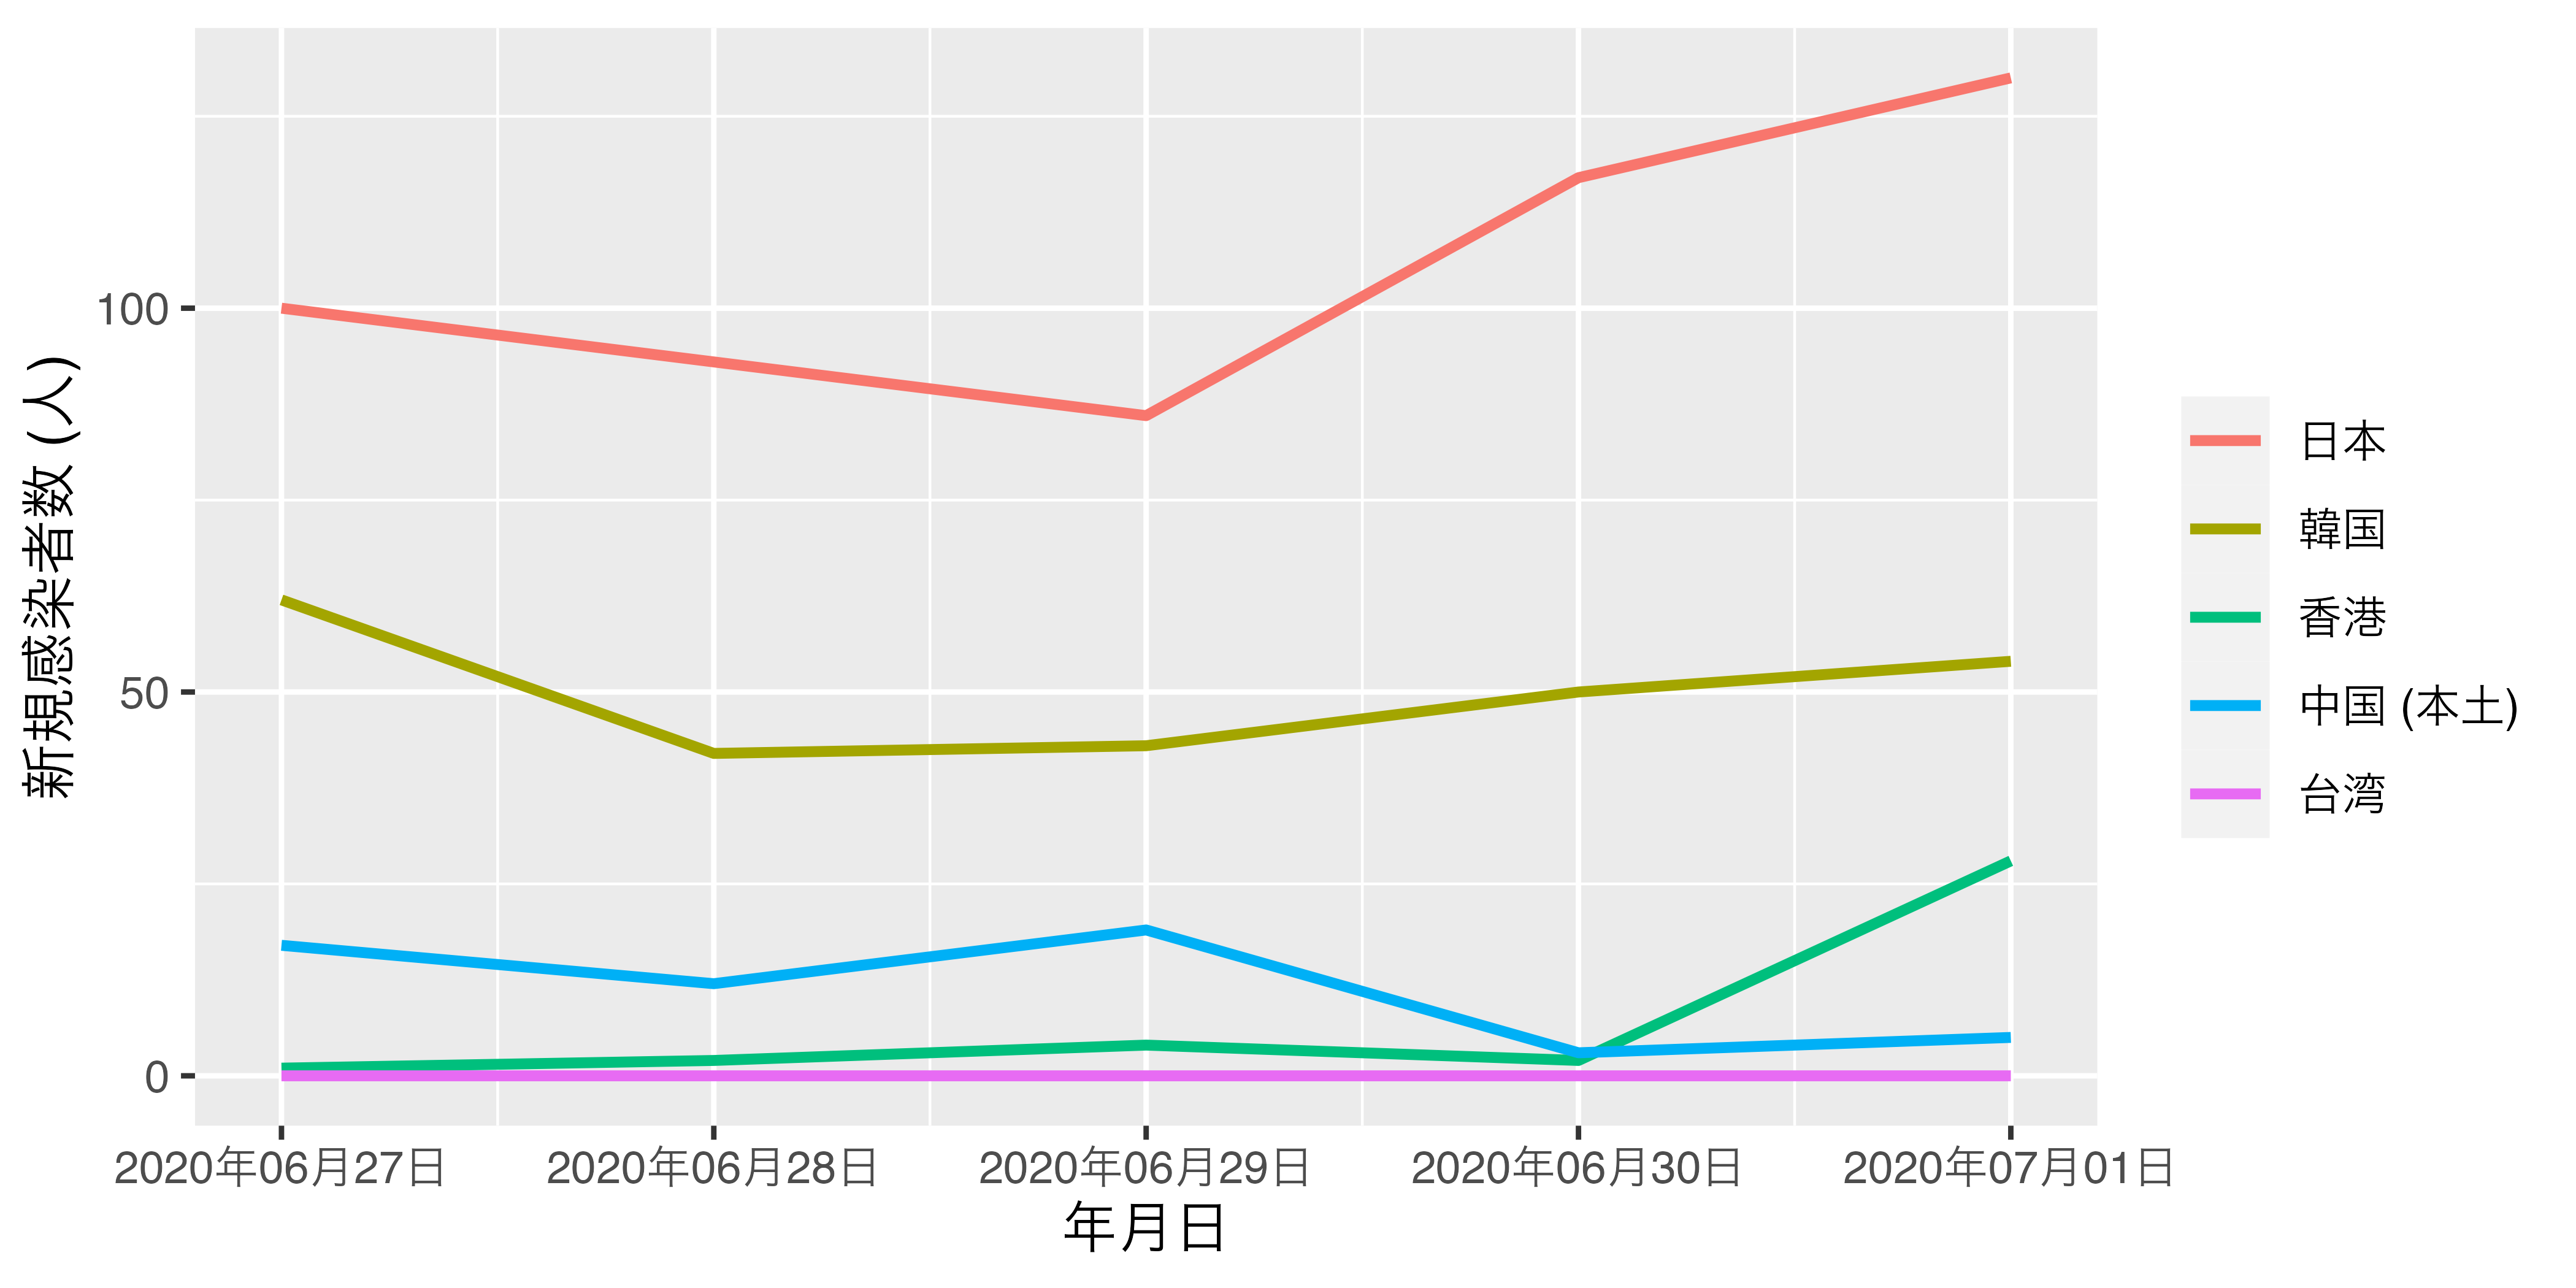
\includegraphics{./functions_files/figure-pdf/unnamed-chunk-46-1.png}

}

\end{figure}

ややギザギザしているように見えますが\footnote{1万個ではなく、100万個、1億個など乱数を生成すればするほど、一様分布に近づきます。}、これなら一様分布だと考えて良いでしょう。

\begin{center}\rule{0.5\linewidth}{0.5pt}\end{center}

\hypertarget{sec-func_exercise}{%
\section{練習問題}\label{sec-func_exercise}}

\textbf{問1}

\begin{itemize}
\tightlist
\item
  長さ2のnumericベクトル\texttt{Data}について考える。条件分岐を用いて\texttt{Data}の1番目の要素
  (\texttt{Data{[}1{]}})が2番目の要素
  (\texttt{Data{[}2{]}})より大きい場合、1番目の要素と2番目の順番を逆転させる条件分岐を作成せよ。たとえば、\texttt{Data\ \textless{}-\ c(5,\ 3)}なら、条件分岐後の\texttt{Data}の値が\texttt{c(3,\ 5)}になること。
\end{itemize}

\textbf{問2}

\begin{itemize}
\tightlist
\item
  与えられた正の実数の平方根を求める\texttt{my\_sqrt()}を作成する。平方根を計算する方法はHero
  of Alexandriaの近似法\footnote{実はこの方法はアレクサンドリアのヘロンが考案したものではないと言われており、もっと昔の古代バビロニアで使用されたと推測される。}を使用する。

  \begin{enumerate}
  \def\labelenumi{\arabic{enumi}.}
  \tightlist
  \item
    平方根を求める\texttt{x}、任意の初期値\texttt{g}、非常に小さい正の実数\texttt{e}を入力する。\texttt{e}の既定値は0.001とする。
  \item
    \texttt{g}の2乗を計算し、\texttt{x\ -\ g\^{}2}の絶対値を\texttt{gap}とする(\texttt{gap}の初期値は\texttt{Inf}とする)。
  \item
    \texttt{gap}が\texttt{e}より小さい場合、\texttt{g}を\texttt{x}の平方根として返す。
  \item
    \texttt{gap}が\texttt{e}より大きい場合、\texttt{g\ +\ (x\ /\ g)}を新しい\texttt{g}とする。
  \item
    2へ戻る。
  \end{enumerate}
\item
  \texttt{while()}関数を使えば簡単である。
\end{itemize}

\begin{Shaded}
\begin{Highlighting}[numbers=left,,]
\CommentTok{\# Rのsqrt()関数}
\FunctionTok{sqrt}\NormalTok{(}\DecValTok{29}\NormalTok{)}
\end{Highlighting}
\end{Shaded}

\begin{verbatim}
[1] 5.385165
\end{verbatim}

\begin{Shaded}
\begin{Highlighting}[numbers=left,,]
\CommentTok{\# 計算例1}
\FunctionTok{my\_sqrt}\NormalTok{(}\DecValTok{29}\NormalTok{, }\DecValTok{5}\NormalTok{) }\CommentTok{\# 29の平方根。初期値は5}
\end{Highlighting}
\end{Shaded}

\begin{verbatim}
[1] 5.385185
\end{verbatim}

\begin{Shaded}
\begin{Highlighting}[numbers=left,,]
\CommentTok{\# 計算例2}
\FunctionTok{my\_sqrt}\NormalTok{(}\DecValTok{29}\NormalTok{, }\DecValTok{5}\NormalTok{, }\AttributeTok{e =} \FloatTok{0.00001}\NormalTok{) }\CommentTok{\# 29の平方根。初期値は5。eは0.00001}
\end{Highlighting}
\end{Shaded}

\begin{verbatim}
[1] 5.385165
\end{verbatim}

\begin{Shaded}
\begin{Highlighting}[numbers=left,,]
\CommentTok{\# 計算例3}
\FunctionTok{my\_sqrt}\NormalTok{(}\SpecialCharTok{{-}}\DecValTok{3}\NormalTok{, }\DecValTok{5}\NormalTok{, }\AttributeTok{e =} \FloatTok{0.00001}\NormalTok{) }\CommentTok{\# あえてエラーを出してみる}
\end{Highlighting}
\end{Shaded}

\begin{verbatim}
Error in my_sqrt(-3, 5, e = 1e-05): xは正の実数でなければなりません。
\end{verbatim}

\textbf{問3}

\begin{itemize}
\tightlist
\item
  問3ではベクトルの1番目要素と2番目の要素を比較し、前者が大きい場合において順番を入れ替える条件分岐を行った。これを長さ3以上のベクトルにも適用したい。長さ4のnumeric型ベクトル\texttt{Data}がある場合の計算手順について考えてみよう。

  \begin{enumerate}
  \def\labelenumi{\arabic{enumi}.}
  \tightlist
  \item
    \texttt{Data{[}1{]}}と\texttt{Data{[}2{]}}の要素を比較し、\texttt{Data{[}1{]}\ \textgreater{}\ Data{[}2{]}}の場合、入れ替える。
  \item
    \texttt{Data{[}2{]}}と\texttt{Data{[}3{]}}の要素を比較し、\texttt{Data{[}2{]}\ \textgreater{}\ Data{[}3{]}}の場合、入れ替える。
  \item
    \texttt{Data{[}3{]}}と\texttt{Data{[}4{]}}の要素を比較し、\texttt{Data{[}3{]}\ \textgreater{}\ Data{[}4{]}}の場合、入れ替える。この段階で\texttt{Data{[}4{]}}は\texttt{Data}の最大値が格納される。
  \item
    続いて、\texttt{Data{[}1{]}}と\texttt{Data{[}2{]}}の要素を比較し、\texttt{Data{[}1{]}\ \textgreater{}\ Data{[}2{]}}の場合、入れ替える。
  \item
    \texttt{Data{[}2{]}}と\texttt{Data{[}3{]}}の要素を比較し、\texttt{Data{[}2{]}\ \textgreater{}\ Data{[}3{]}}の場合、入れ替える。この段階で\texttt{Data{[}3{]}}には\texttt{Data}の2番目に大きい数値が格納される。
  \item
    最後に\texttt{Data{[}1{]}}と\texttt{Data{[}2{]}}の要素を比較し、\texttt{Data{[}1{]}\ \textgreater{}\ Data{[}2{]}}の場合、入れ替える。ここで並び替えは終了
  \end{enumerate}
\item
  \textbf{ヒント:}
  2つの\texttt{for()}文が必要となる。これは「\href{https://ja.wikipedia.org/wiki/バブルソート}{バブルソート}」と呼ばれる最も簡単なソートアルゴリズムである。イメージとしては、長さNのベクトルの場合、n番目の要素とn+1番目の要素を比較しながら、大きい方を後ろの方に追い込む形である。最初は、\texttt{Data{[}4{]}}最後の要素に最大値を格納し、続いて、\texttt{Data{[}3{]}}に次に大きい数値を、\texttt{Data{[}2{]}}に次に大きい数値を入れる仕組みである。

  \begin{itemize}
  \tightlist
  \item
    最初は\texttt{Data{[}1{]}}と\texttt{Data{[}2{]}}、\texttt{Data{[}2{]}}と\texttt{Data{[}3{]}}、\texttt{Data{[}3{]}}と\texttt{Data{[}4{]}}の3ペアの比較を行う。
  \item
    続いて、\texttt{Data{[}1{]}}と\texttt{Data{[}2{]}}、\texttt{Data{[}2{]}}と\texttt{Data{[}3{]}}の2ペアの比較を行う
  \item
    最後に、\texttt{Data{[}1{]}}と\texttt{Data{[}2{]}}の1ペアの比較を行う
  \item
    つまり、外側の\texttt{for()}文は「\texttt{Data}の長さ-1」回繰り返すことになる。
  \item
    内側の\texttt{for()}文は3, 2, 1ペアの比較を行うことになる。
  \end{itemize}
\end{itemize}

\textbf{問4}

\begin{itemize}
\tightlist
\item
  「問4」の練習問題で作成したコードを関数化せよ。関数名は\texttt{mySort()}であり、引数は長さ2以上のnumeric型ベクトルのみである。引数名は自由に決めても良いし、\texttt{data}や\texttt{x}などを使っても良い。
\end{itemize}

\textbf{問5}

\begin{itemize}
\tightlist
\item
  既に作成した\texttt{DQ\_Attack}関数を修正してみよう。今の関数は通常攻撃のみであるが、稀に「会心の一撃」が発生するように修正する。

  \begin{itemize}
  \tightlist
  \item
    会心の一撃が発生する確率は1/32とする (Hint:
    0から1の間の乱数を生成し、その乱数が1/32以下であるか否かで条件分岐させる)。乱数の生成は\texttt{runif()}または、自作関数の\texttt{LCG()}でも良い。
  \item
    会心の一撃のダメージの最小値は攻撃力の95\%、最大値は105\%とする。
  \item
    会心の一撃が発生したら、\texttt{"かいしんのいちげき!\ スライムに10のダメージ!!"}のようなメッセージを出力させること。
  \end{itemize}
\end{itemize}

\textbf{問6}

\begin{itemize}
\tightlist
\item
  与えられたベクトル\texttt{x}から\texttt{n}個の要素を無作為に抽出する関数、\texttt{mySample()}を定義せよ。\texttt{mySample()}の引数は\texttt{x}と\texttt{n}、\texttt{seed}とし、\texttt{x}は長さ1以上のベクトルとする。\texttt{n}は長さ1の整数型ベクトルである。

  \begin{itemize}
  \tightlist
  \item
    以下の場合、エラーメッセージを出力し、処理を中止させること。

    \begin{itemize}
    \tightlist
    \item
      \texttt{n}と\texttt{seed}が長さ1ベクトルでない場合、
    \item
      \texttt{seed}がnumeric型でない場合
    \item
      \texttt{n}が整数でない場合 (\texttt{floor(n)\ ==\ n}で判定)
    \end{itemize}
  \item
    \textbf{ヒント:}
    \texttt{LCG()}関数を用いて乱数を生成した場合、生成された擬似乱数は0以上1以下である。ベクトル\texttt{x}の長さを\texttt{length(x)}とした場合、擬似乱数に\texttt{length(x)}を掛けると、擬似乱数は0以上\texttt{length(x)}以下になる。これらの値を切り上げると
    (\texttt{ceiling()}関数)、その値は1以上\texttt{length(x)}以下の整数となる。
  \end{itemize}
\end{itemize}

\part{データハンドリング}

\hypertarget{sec-datahandling1}{%
\chapter{データハンドリング {[}抽出{]}}\label{sec-datahandling1}}

ここでは比較的綺麗に整形されているデータフレームを扱う方法について考えます。ここでいう「比較的綺麗なデータ」とは、すぐに分析に使えるレベルのデータを意味します。したがって、ここではデータ内の値を変更するような作業は行いません。基本的に分析しやすくなるように列の順番を替えたり、特定の列や行のみを抽出したり、データの順番を並び替える作業に注目します。

本章では以下の3つの内容を中心に解説します。

\begin{enumerate}
\def\labelenumi{\arabic{enumi}.}
\tightlist
\item
  パイプ演算子 (\texttt{\%\textgreater{}\%})に慣れる
\item
  特定の行と列の抽出
\item
  データのソート
\end{enumerate}

本章で学習する内容でデータを加工した場合、得られる結果物は元のデータの一部
(subset)となります。データの中身の値を変えたり、新しい列を追加したり、平均値などの記述統計量をまとめたりする方法については次の第\ref{sec-datahandling2}章で解説します。

\begin{center}\rule{0.5\linewidth}{0.5pt}\end{center}

\hypertarget{sec-handling1_intro}{%
\section{データハンドリングとtidyverse}\label{sec-handling1_intro}}

\begin{quote}
The tidyverse is an opinionated collection of R packages designed for
data science. All packages share an underlying design philosophy,
grammar, and data structures. (Tidyverseホームページから)
\end{quote}

Tidyverseとはデータサイエンスのために考案された、強い信念と思想に基づいたRパッケージの集合です。Tidyverseに属するパッケージは思想、文法およびデータ構造を共有しています。Tidyverseの中核をなすパッケージは\{ggplot2\}(第\ref{sec-visualization1}、\ref{sec-visualization2}、\ref{sec-visualization3}、\ref{sec-visualization4}章)、\{dplyr\}(第\ref{sec-datahandling1}、\ref{sec-datahandling2}章)、\{tidyr\}(第\ref{sec-tidydata}章)、\{readr\}(第\ref{sec-io_read}章)、\{purrr\}
(第\ref{sec-iteration}章)、\{tibble\}(第\ref{sec-datastructure_dataframe}章)、\{stringr\}
(第\ref{sec-string}章)、\{forcats\}
(第\ref{sec-factor}章)などがあり、このパッケージを支える数十のパッケージが含まれています。これらのパッケージは個別に読み込む必要はなく、\{tidyverse\}パッケージを読み込むだけで十分です。

\begin{Shaded}
\begin{Highlighting}[numbers=left,,]
\FunctionTok{library}\NormalTok{(tidyverse)}
\end{Highlighting}
\end{Shaded}

\begin{verbatim}
-- Attaching packages --------------------------------------- tidyverse 1.3.1 --
\end{verbatim}

\begin{verbatim}
v ggplot2 3.3.5     v purrr   0.3.4
v tibble  3.1.6     v dplyr   1.0.8
v tidyr   1.2.0     v stringr 1.4.0
v readr   2.1.2     v forcats 0.5.1
\end{verbatim}

\begin{verbatim}
-- Conflicts ------------------------------------------ tidyverse_conflicts() --
x dplyr::filter() masks stats::filter()
x dplyr::lag()    masks stats::lag()
\end{verbatim}

Rにおけるデータハンドリング
(データ操作)の標準が\{dplyr\}と\{tidyr\}中心となり、文字列の処理は\{stringr\}、factor型の操作は\{forcats\}、大量のモデルを自動的に分析し、結果を処理するためには\{tibble\}と\{purrr\}、可視化は\{ggplot2\}が主に使われています。これらのパッケージ間、あるいはパッケージ内におけるオブジェクトのやり取りは全てパイプ演算子を通じて行われています。また、これらのパッケージは整然データ
(tidydata)を想定するか、整然データの作成するに特化しています。

tidyverseの思想に基づいた「tidyverse流のコーディング」は現在のRそのものと言っても過言ではありません。ただし、tidyverseじゃないと出来ないデータハンドリング、可視化などはありません。tidyverseはデータサイエンスの思想に近いものであり、「異なる思想を持っているからこのような分析はできない」といったものはありません。tidyverseという概念が提唱される前にもRは存在し、tidyverse無き世界で今と同じことをやってきました。ただし、tidyverse流で書かれたRコードは可読性が優れ、コードを書く手間も短くなります。tidyverseの考え方がRのける「標準語」として定着しつつあるのは否めない事実であり、学習する誘引としては十分すぎるでしょう。

\begin{center}\rule{0.5\linewidth}{0.5pt}\end{center}

\hypertarget{sec-handling1_pipe}{%
\section{\texorpdfstring{パイプ演算子
(\texttt{\%\textgreater{}\%})}{パイプ演算子 (\%\textgreater\%)}}\label{sec-handling1_pipe}}

\{dplyr\}パッケージを利用する前にパイプ演算子について説明します。パイプ演算子は\{dplyr\}に含まれている演算子ではなく、\{magrittr\}という別のパッケージから提供される演算子ですが、\{tidyverse\}パッケージを読み込むと自動的に読み込まれます。パイプ演算子は\texttt{x\ \%\textgreater{}\%\ y()}のような書き方となりますが、これは「\texttt{x}を\texttt{y()}の第一引数として渡す」ことを意味します。\texttt{x}の部分はベクトルやデータフレームのようなオブジェクトでも、関数でも構いません。なぜなら、関数から得られた結果もまたベクトルやデータフレームといったものになるからです。つまり、\texttt{x()\ \%\textgreater{}\%\ y()}という使い方も可能です。そして、パイプは無限に繋ぐこともできます。「データ\texttt{df}を関数\texttt{x()}で処理をし、その結果をまた関数\texttt{y()}で処理する」ことは、パイプを使うと\texttt{df\ \%\textgreater{}\%\ x()\ \%\textgreater{}\%\ y()}のような書き方となります。

たとえば、「\texttt{paste(3,\ "+",\ 5,\ "=",\ 8)}を実行し、その結果を\texttt{rep()}関数を使って3回複製し、それを\texttt{print()}を使って出力する」コードを考えてみましょう。方法としては2つ考えられます。まずは、それぞれの処理を別途のオブジェクトに格納する方法です。そして二つ目は関数の中に関数を使う方法です。

\begin{Shaded}
\begin{Highlighting}[numbers=left,,]
\CommentTok{\# 方法1: 一関数一オブジェクト}
\NormalTok{Result1 }\OtherTok{\textless{}{-}} \FunctionTok{paste}\NormalTok{(}\DecValTok{3}\NormalTok{, }\StringTok{"+"}\NormalTok{, }\DecValTok{5}\NormalTok{, }\StringTok{"="}\NormalTok{, }\DecValTok{8}\NormalTok{)}
\NormalTok{Result2 }\OtherTok{\textless{}{-}} \FunctionTok{rep}\NormalTok{(Result1, }\DecValTok{3}\NormalTok{)}
\FunctionTok{print}\NormalTok{(Result2)}
\end{Highlighting}
\end{Shaded}

\begin{verbatim}
[1] "3 + 5 = 8" "3 + 5 = 8" "3 + 5 = 8"
\end{verbatim}

\begin{Shaded}
\begin{Highlighting}[numbers=left,,]
\CommentTok{\# 方法2: 関数の中に関数の中に関数}
\FunctionTok{print}\NormalTok{(}\FunctionTok{rep}\NormalTok{(}\FunctionTok{paste}\NormalTok{(}\DecValTok{3}\NormalTok{, }\StringTok{"+"}\NormalTok{, }\DecValTok{5}\NormalTok{, }\StringTok{"="}\NormalTok{, }\DecValTok{8}\NormalTok{), }\DecValTok{3}\NormalTok{))}
\end{Highlighting}
\end{Shaded}

\begin{verbatim}
[1] "3 + 5 = 8" "3 + 5 = 8" "3 + 5 = 8"
\end{verbatim}

どれも結果は同じです。コードを書く手間を考えれば、後者の方が楽かも知れませんが、可読性があまりよくありません。一方、前者は可読性は良いものの、コードも長くなり、オブジェクトを2つも作ってしまうのでメモリの無駄遣いになります。

コードの可読性と書く手間、両方を満足する書き方がパイプ演算子\texttt{\%\textgreater{}\%}です。まずは、例から見ましょう。

\begin{Shaded}
\begin{Highlighting}[numbers=left,,]
\CommentTok{\# \%\textgreater{}\%を使う}
\FunctionTok{paste}\NormalTok{(}\DecValTok{3}\NormalTok{, }\StringTok{"+"}\NormalTok{, }\DecValTok{5}\NormalTok{, }\StringTok{"="}\NormalTok{, }\DecValTok{8}\NormalTok{) }\SpecialCharTok{\%\textgreater{}\%} \FunctionTok{rep}\NormalTok{(}\DecValTok{3}\NormalTok{) }\SpecialCharTok{\%\textgreater{}\%} \FunctionTok{print}\NormalTok{()}
\end{Highlighting}
\end{Shaded}

\begin{verbatim}
[1] "3 + 5 = 8" "3 + 5 = 8" "3 + 5 = 8"
\end{verbatim}

まず、結果は先ほどと同じです。それではコードの説明をしましょう。まずは、\texttt{paste(3,\ "+",\ 5,\ "=",\ 8)}を実行します。そしてその結果をそのまま\texttt{rep()}関数の第一引数として渡されます。つまり、\texttt{rep(paste(3,\ "+",\ 5,\ "=",\ 8),\ 3)}になるわけです。ここでは\texttt{rep(3)}と書きましたが、第一引数が渡されたため、\texttt{3}は第二引数扱いになります
(パイプ演算子前のオブジェクトを第二、三引数として渡す方法は適宜説明します。)。そして、これをまた\texttt{print()}関数に渡します。結果としては\texttt{print(rep(paste(3,\ "+",\ 5,\ "=",\ 8),\ 3))}となります。

関数を重ねると読む順番は「カッコの内側から外側へ」になりますが、パイプ演算子を使うと「左
(上)から右
(下)へ」といったより自然な読み方が可能になります。また、以下のコードのように、パイプ演算子後に改行を行うことでより読みやすいコードになります。これからはパイプ演算子の後は必ず改行をします。

\begin{Shaded}
\begin{Highlighting}[numbers=left,,]
\CommentTok{\# 改行 (+字下げ)したらもっと読みやすくなる}
\FunctionTok{paste}\NormalTok{(}\DecValTok{3}\NormalTok{, }\StringTok{"+"}\NormalTok{, }\DecValTok{5}\NormalTok{, }\StringTok{"="}\NormalTok{, }\DecValTok{8}\NormalTok{) }\SpecialCharTok{\%\textgreater{}\%} 
    \FunctionTok{rep}\NormalTok{(}\DecValTok{3}\NormalTok{) }\SpecialCharTok{\%\textgreater{}\%} 
    \FunctionTok{print}\NormalTok{()}
\end{Highlighting}
\end{Shaded}

パイプ演算子を使わない方法 図~\ref{fig-handling1_pipe1}
のようにイメージできます。一回の処理ごとに結果を保存し、それをまた次の処理時においてデータとして使うイメージです。

\begin{figure}

{\centering 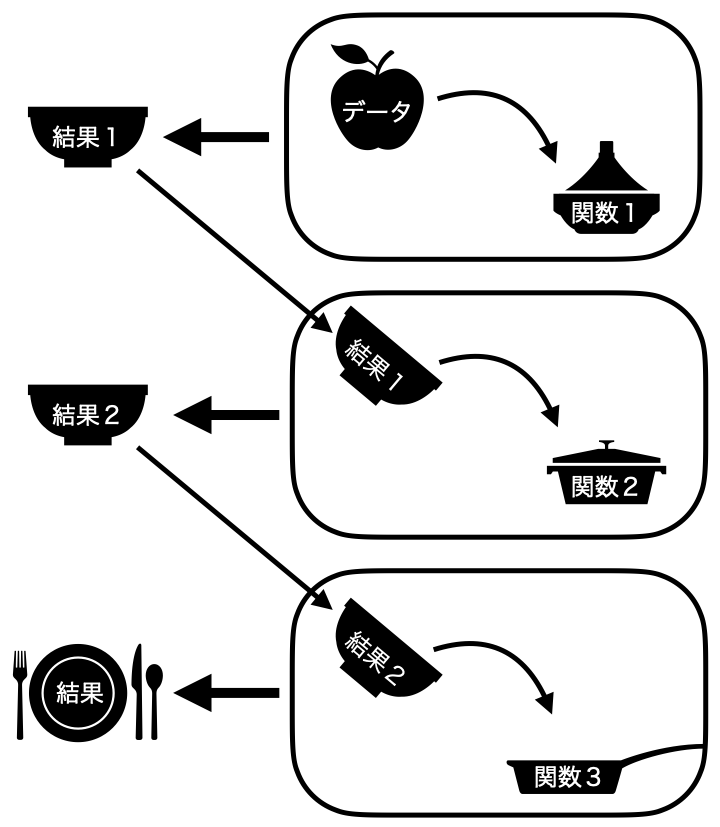
\includegraphics[width=0.75\textwidth,height=\textheight]{./Figs/Handling1/Pipeline1.png}

}

\caption{\label{fig-handling1_pipe1}パイプ演算子を使わない場合}

\end{figure}

一方、 図~\ref{fig-handling1_pipe2}
はパイプ演算子を使う場合のプロセスです。処理後の結果を保存せず、すぐに次のプロセスに渡すことで、メモリ
(図だとボウル)や時間、コードの無駄を減らすことができます。むろん、
図~\ref{fig-handling1_pipe1}
の結果1を使って色々試してみたい場合は、一旦結果1までは格納し、適宜引き出して使った方が効率的でしょう。パイプ演算子はたしかに便利で、「今どき」のRの書き方を象徴するようなものですが、一つの結果を出すまであまりにも多くのパイプ演算子を使うことはあ望ましくありません。

\begin{figure}

{\centering 
\includegraphics[width=0.75\textwidth,height=\textheight]{./Figs/Handling1/Pipeline2.png}

}

\caption{\label{fig-handling1_pipe2}パイプ演算子を使う場合}

\end{figure}

データハンドリングもこれど同様に、様々な作業を順に沿って行う必要があります。例えば、「(1)
列を選択して、(2) 欠損値を含む列を除去して、 (3)
ある変数の値を100倍にして、(4)
ある変数の値がが小さい行から大きい順へ並び替える」といった手順です。これらの作業はパイプ演算子を使えば、スムーズに行うことが可能です。

\hypertarget{sec-handling1_select}{%
\section{列の抽出}\label{sec-handling1_select}}

それでは今回の実習用データを読み込みましょう。\href{Data/Ramen.csv}{Ramen.csv}には「\href{https://www.gnavi.co.jp}{ぐるなび}」から取得したラーメン屋6292店舗の情報が入っています。具体的には東京、神奈川、千葉、埼玉、大阪、京都、兵庫、奈良、和歌山それぞれ都府県にあるラーメン屋の中から最大1000店舗の情報を抽出したものです。東京都は、ぐるなびに登録したラーメン屋が3000店舗以上ですが、1000店舗の基準はぐるなびの「おすすめ」の順で上位1000店舗となります。また、店側またはぐるなびが登録したカテゴリを基準に抽出したため、実際はラーメン屋ではないにもかかわらずラーメン屋としてデータ内に含まれている可能性があります。

まず、このデータを読み込み、\texttt{df}という名付けます。

\begin{Shaded}
\begin{Highlighting}[numbers=left,,]
\NormalTok{df }\OtherTok{\textless{}{-}} \FunctionTok{read\_csv}\NormalTok{(}\StringTok{"Data/Ramen.csv"}\NormalTok{)}
\end{Highlighting}
\end{Shaded}

\begin{verbatim}
Rows: 6292 Columns: 14
-- Column specification --------------------------------------------------------
Delimiter: ","
chr (5): ID, Name, Pref, Line, Station
dbl (9): Zipcode, Latitude, Longitude, Walk, Bus, Car, Budget, ScoreN, Score

i Use `spec()` to retrieve the full column specification for this data.
i Specify the column types or set `show_col_types = FALSE` to quiet this message.
\end{verbatim}

データの中身を確認してみましょう。

\begin{Shaded}
\begin{Highlighting}[numbers=left,,]
\NormalTok{df}
\end{Highlighting}
\end{Shaded}

\begin{verbatim}
# A tibble: 6,292 x 14
   ID     Name  Pref  Zipcode Latitude Longitude Line  Station  Walk   Bus   Car
   <chr>  <chr> <chr>   <dbl>    <dbl>     <dbl> <chr> <chr>   <dbl> <dbl> <dbl>
 1 e5396~ 居酒~ 東京~ 1040031     35.7      140. 地下~ 銀座一~     3    NA    NA
 2 gfeb6~ 本格~ 東京~ 1100005     35.7      140. 地下~ 仲御徒~     1    NA    NA
 3 ggt59~ 食べ~ 東京~ 1250041     35.8      140. JR~ 金町駅      2    NA    NA
 4 g1813~ 博多~ 東京~ 1920904     35.7      139. JR  八王子~     1    NA    NA
 5 ggww1~ まさ~ 東京~ 1500042     35.7      140. 地下~ 渋谷駅      7    NA    NA
 6 gdzk5~ 完全~ 東京~ 1000013     35.7      140. 地下~ 虎ノ門~     3    NA    NA
 7 ga2g2~ 鶏そ~ 東京~ 1760006     35.7      140. 西武~ 江古田~     2    NA    NA
 8 gg9m1~ 宴会~ 東京~ 1010021     35.7      140. JR  秋葉原~     4    NA    NA
 9 gdvk2~ 中国~ 東京~ 1000006     35.7      140. JR  有楽町~     1    NA    NA
10 gggb2~ 中国~ 東京~ 1140002     35.8      140. 地下~ 王子駅      2    NA    NA
# ... with 6,282 more rows, and 3 more variables: Budget <dbl>, ScoreN <dbl>,
#   Score <dbl>
\end{verbatim}

1行目の\texttt{\#\ A\ tibble:\ 2,000\ x\ 12}から、ケース数
(店舗数)は2000、変数は12個あることが分かります。各変数の詳細は
表~\ref{tbl-handling1_dataset} の通りです。

\hypertarget{tbl-handling1_dataset}{}
\begin{table}
\caption{\label{tbl-handling1_dataset}Ramen.csvの詳細 }

\centering
\begin{tabular}{l|l}
\hline
\multicolumn{1}{c}{変数名} & \multicolumn{1}{c}{説明}\\
\hline
`ID` & 店舗ID\\
\hline
`Name` & 店舗名\\
\hline
`Pref` & 店舗の所在地 (都府県)\\
\hline
`Zipcode` & 店舗の郵便番号\\
\hline
`Latitude` & 緯度\\
\hline
`Longitude` & 経度\\
\hline
`Line` & 最寄りの駅の路線\\
\hline
`Station` & 最寄りの駅\\
\hline
`Walk` & 最寄りの駅からの距離 (徒歩; 分)\\
\hline
`Bus` & 最寄りの駅からの距離 (バス; 分)\\
\hline
`Car` & 最寄りの駅からの距離 (車; 分)\\
\hline
`Budget` & 平均予算 (円)\\
\hline
`ScoreN` & 口コミの数\\
\hline
`Score` & 口コミ評価の平均値\\
\hline
\end{tabular}
\end{table}

それではここからは\texttt{df}を用いた\{dplyr\}の様々な機能を紹介していきます。

\hypertarget{ux7279ux5b9aux306eux5217ux3092ux62bdux51faux3059ux308b}{%
\subsection{特定の列を抽出する}\label{ux7279ux5b9aux306eux5217ux3092ux62bdux51faux3059ux308b}}

まずは、データフレームから特定の列のみを残す、除去する方法について紹介します。たとえば、\texttt{df}から\texttt{ID}、\texttt{Name}、\texttt{Pref}、\texttt{Score}のみを残すとします。\{dplyr\}を使わない方法と\{dplyr\}の\texttt{select()}関数を使った方法を紹介します。

\begin{Shaded}
\begin{Highlighting}[numbers=left,,]
\CommentTok{\# dplyrを使わない方法}
\NormalTok{df[, }\FunctionTok{c}\NormalTok{(}\StringTok{"ID"}\NormalTok{, }\StringTok{"Name"}\NormalTok{, }\StringTok{"Pref"}\NormalTok{, }\StringTok{"Score"}\NormalTok{)]}
\end{Highlighting}
\end{Shaded}

\begin{verbatim}
# A tibble: 6,292 x 4
   ID      Name                                                     Pref   Score
   <chr>   <chr>                                                    <chr>  <dbl>
 1 e539604 居酒屋 龍記 京橋店                                       東京都 NA   
 2 gfeb600 本格上海料理 新錦江 上野御徒町本店                       東京都  4.5 
 3 ggt5900 食べ飲み放題×中華ビストロ NOZOMI(のぞみ)               東京都 NA   
 4 g181340 博多餃子軒 八王子店 タピオカ店 Bull Pulu(ブルプル)併設 東京都 NA   
 5 ggww100 まさ屋 渋谷店                                            東京都 NA   
 6 gdzk500 完全個室 上海レストラン 檸檬 霞ヶ関ビル内店              東京都 NA   
 7 ga2g202 鶏そば きらり                                            東京都 NA   
 8 gg9m100 宴会個室×餃子酒場 北京飯店 秋葉原本店                    東京都  3.33
 9 gdvk200 中国料理 宝龍                                            東京都  2.5 
10 gggb200 中国料理 天安門                                          東京都 NA   
# ... with 6,282 more rows
\end{verbatim}

\begin{Shaded}
\begin{Highlighting}[numbers=left,,]
\CommentTok{\# dplyr::select()を使う方法}
\CommentTok{\# select(df, ID, Name, Pref, Score)でもOK}
\NormalTok{df }\SpecialCharTok{\%\textgreater{}\%}
  \FunctionTok{select}\NormalTok{(ID, Name, Pref, Score)}
\end{Highlighting}
\end{Shaded}

\begin{verbatim}
# A tibble: 6,292 x 4
   ID      Name                                                     Pref   Score
   <chr>   <chr>                                                    <chr>  <dbl>
 1 e539604 居酒屋 龍記 京橋店                                       東京都 NA   
 2 gfeb600 本格上海料理 新錦江 上野御徒町本店                       東京都  4.5 
 3 ggt5900 食べ飲み放題×中華ビストロ NOZOMI(のぞみ)               東京都 NA   
 4 g181340 博多餃子軒 八王子店 タピオカ店 Bull Pulu(ブルプル)併設 東京都 NA   
 5 ggww100 まさ屋 渋谷店                                            東京都 NA   
 6 gdzk500 完全個室 上海レストラン 檸檬 霞ヶ関ビル内店              東京都 NA   
 7 ga2g202 鶏そば きらり                                            東京都 NA   
 8 gg9m100 宴会個室×餃子酒場 北京飯店 秋葉原本店                    東京都  3.33
 9 gdvk200 中国料理 宝龍                                            東京都  2.5 
10 gggb200 中国料理 天安門                                          東京都 NA   
# ... with 6,282 more rows
\end{verbatim}

どれも結果は同じですが、\texttt{select()}関数を使った方がより読みやすいコードになっているでしょう。むろん、\texttt{select()}関数を使わない方がスッキリする方も知るかも知れません。実際、自分でパッケージなどを作成する際は\texttt{select()}を使わない場合が多いです。ただし、一般的な分析の流れでは\texttt{select()}の方がコードも意味も明確となり、パイプ演算子でつなぐのも容易です。

\texttt{select()}関数の使い方は非常に簡単です。第一引数はデータフレームですが、パイプ演算子を使う場合は省略可能です。第二引数以降の引数はデータフレームの変数名です。つまり、ここには残す変数名のみを書くだけで十分です。

また、\texttt{select()}関数を使って列の順番を変えることもできます。たとえば、\texttt{ID}、\texttt{Pref}、\texttt{Name}、\texttt{Score}の順で列を残すなら、この順番で引数を書くだけです。

\begin{Shaded}
\begin{Highlighting}[numbers=left,,]
\NormalTok{df }\SpecialCharTok{\%\textgreater{}\%}
  \FunctionTok{select}\NormalTok{(ID, Pref, Name)}
\end{Highlighting}
\end{Shaded}

\begin{verbatim}
# A tibble: 6,292 x 3
   ID      Pref   Name                                                    
   <chr>   <chr>  <chr>                                                   
 1 e539604 東京都 居酒屋 龍記 京橋店                                      
 2 gfeb600 東京都 本格上海料理 新錦江 上野御徒町本店                      
 3 ggt5900 東京都 食べ飲み放題×中華ビストロ NOZOMI(のぞみ)              
 4 g181340 東京都 博多餃子軒 八王子店 タピオカ店 Bull Pulu(ブルプル)併設
 5 ggww100 東京都 まさ屋 渋谷店                                           
 6 gdzk500 東京都 完全個室 上海レストラン 檸檬 霞ヶ関ビル内店             
 7 ga2g202 東京都 鶏そば きらり                                           
 8 gg9m100 東京都 宴会個室×餃子酒場 北京飯店 秋葉原本店                   
 9 gdvk200 東京都 中国料理 宝龍                                           
10 gggb200 東京都 中国料理 天安門                                         
# ... with 6,282 more rows
\end{verbatim}

\hypertarget{ux7279ux5b9aux306eux5217ux3092ux62bdux51faux3057ux5217ux540dux3092ux5909ux66f4ux3059ux308b}{%
\subsection{特定の列を抽出し、列名を変更する}\label{ux7279ux5b9aux306eux5217ux3092ux62bdux51faux3057ux5217ux540dux3092ux5909ux66f4ux3059ux308b}}

また、特定の列を残す際、変数名を変更することも可能です。今回も\texttt{ID}、\texttt{Name}、\texttt{Pref}、\texttt{Score}のみを残しますが、\texttt{Pref}列は\texttt{Prefecture}に変えてみましょう。

\begin{Shaded}
\begin{Highlighting}[numbers=left,,]
\NormalTok{df }\SpecialCharTok{\%\textgreater{}\%}
  \FunctionTok{select}\NormalTok{(ID, Name, }\AttributeTok{Prefecture =}\NormalTok{ Pref, Score)}
\end{Highlighting}
\end{Shaded}

\begin{verbatim}
# A tibble: 6,292 x 4
   ID      Name                                                Prefecture Score
   <chr>   <chr>                                               <chr>      <dbl>
 1 e539604 居酒屋 龍記 京橋店                                  東京都     NA   
 2 gfeb600 本格上海料理 新錦江 上野御徒町本店                  東京都      4.5 
 3 ggt5900 食べ飲み放題×中華ビストロ NOZOMI(のぞみ)          東京都     NA   
 4 g181340 博多餃子軒 八王子店 タピオカ店 Bull Pulu(ブルプル~ 東京都     NA   
 5 ggww100 まさ屋 渋谷店                                       東京都     NA   
 6 gdzk500 完全個室 上海レストラン 檸檬 霞ヶ関ビル内店         東京都     NA   
 7 ga2g202 鶏そば きらり                                       東京都     NA   
 8 gg9m100 宴会個室×餃子酒場 北京飯店 秋葉原本店               東京都      3.33
 9 gdvk200 中国料理 宝龍                                       東京都      2.5 
10 gggb200 中国料理 天安門                                     東京都     NA   
# ... with 6,282 more rows
\end{verbatim}

抽出する際、変数を\texttt{新しい変数名\ =\ 既存の変数名}にするだけで、変数名が簡単に変更できました。もし、特定の列は抽出しないものの、変数名を変えるにはどうすれば良いでしょうか。ここでは\texttt{df}の\texttt{Pref}を\texttt{Prefecture}に、\texttt{Walk}を\texttt{Distance}に変更してみます。\{dplyr\}を使わない場合と\{dplyr\}の\texttt{rename()}関数を使う場合を両方紹介します。

まずは、\texttt{name()}関数についてですが、これはデータフレームの変数名をベクトルとして出力する関数です。

\begin{Shaded}
\begin{Highlighting}[numbers=left,,]
\FunctionTok{names}\NormalTok{(df)}
\end{Highlighting}
\end{Shaded}

\begin{verbatim}
 [1] "ID"        "Name"      "Pref"      "Zipcode"   "Latitude"  "Longitude"
 [7] "Line"      "Station"   "Walk"      "Bus"       "Car"       "Budget"   
[13] "ScoreN"    "Score"    
\end{verbatim}

察しの良い読者は気づいたかも知れませんが、\texttt{names(データフレーム名)}の結果はベクトルであり、上書きも可能です。つまり、\texttt{names(df)}の3番目と9番目の要素を\texttt{"Prefecture"}と\texttt{"Distance"}に上書きすることができるということです。

\begin{Shaded}
\begin{Highlighting}[numbers=left,,]
\CommentTok{\# dplyrを使わずに列名を変更する方法}
\FunctionTok{names}\NormalTok{(df)[}\FunctionTok{c}\NormalTok{(}\DecValTok{3}\NormalTok{, }\DecValTok{9}\NormalTok{)] }\OtherTok{\textless{}{-}} \FunctionTok{c}\NormalTok{(}\StringTok{"Prefecture"}\NormalTok{, }\StringTok{"Distance"}\NormalTok{)}

\CommentTok{\# dfの中身を出力}
\NormalTok{df}
\end{Highlighting}
\end{Shaded}

\begin{verbatim}
# A tibble: 6,292 x 14
   ID      Name     Prefecture Zipcode Latitude Longitude Line  Station Distance
   <chr>   <chr>    <chr>        <dbl>    <dbl>     <dbl> <chr> <chr>      <dbl>
 1 e539604 居酒屋 ~ 東京都     1040031     35.7      140. 地下~ 銀座一~        3
 2 gfeb600 本格上~  東京都     1100005     35.7      140. 地下~ 仲御徒~        1
 3 ggt5900 食べ飲~  東京都     1250041     35.8      140. JR~ 金町駅         2
 4 g181340 博多餃~  東京都     1920904     35.7      139. JR  八王子~        1
 5 ggww100 まさ屋 ~ 東京都     1500042     35.7      140. 地下~ 渋谷駅         7
 6 gdzk500 完全個~  東京都     1000013     35.7      140. 地下~ 虎ノ門~        3
 7 ga2g202 鶏そば ~ 東京都     1760006     35.7      140. 西武~ 江古田~        2
 8 gg9m100 宴会個~  東京都     1010021     35.7      140. JR  秋葉原~        4
 9 gdvk200 中国料~  東京都     1000006     35.7      140. JR  有楽町~        1
10 gggb200 中国料~  東京都     1140002     35.8      140. 地下~ 王子駅         2
# ... with 6,282 more rows, and 5 more variables: Bus <dbl>, Car <dbl>,
#   Budget <dbl>, ScoreN <dbl>, Score <dbl>
\end{verbatim}

簡単に変数名の変更ができました。続いて、\{dplyr\}の\texttt{rename()}関数を使った方法です。今回は、\texttt{Prefecture}を\texttt{Pref}に、\texttt{Distance}を\texttt{Walk}に戻して見ましょう。そして、出力するだけにとどまらず、\texttt{df}に上書きしましょう。

\begin{Shaded}
\begin{Highlighting}[numbers=left,,]
\CommentTok{\# dfのPrefectureをPrefに、DistanceをWalkに変更し、上書きする}
\NormalTok{df }\OtherTok{\textless{}{-}}\NormalTok{ df }\SpecialCharTok{\%\textgreater{}\%}
  \FunctionTok{rename}\NormalTok{(}\AttributeTok{Pref =}\NormalTok{ Prefecture, }\AttributeTok{Walk =}\NormalTok{ Distance)}
\end{Highlighting}
\end{Shaded}

これで終わりです。実は\texttt{select()}関数と使い方がほぼ同じです。ただし、残す変数名を指定する必要がなく、名前を変更する変数名と新しい変数名を入れるだけです。変数が少ないデータなら\texttt{select()}でもあまり不便は感じないかも知れませんが、変数が多くなると\texttt{rename()}関数は非常に便利です。

\hypertarget{ux7279ux5b9aux306eux5217ux3092ux9664ux5916ux3059ux308b}{%
\subsection{特定の列を除外する}\label{ux7279ux5b9aux306eux5217ux3092ux9664ux5916ux3059ux308b}}

逆に、一部の変数をデータフレームから除去したい場合もあるでしょう。たとえば、緯度
(\texttt{Latitude})と経度
(\texttt{Longitude})はラーメン屋の情報としては不要かもしれません。この2つの変数を除外するためにはどうすれば良いでしょうか。まず考えられるのは、この2つの変数を除いた変数を指定・抽出する方法です。

\begin{Shaded}
\begin{Highlighting}[numbers=left,,]
\NormalTok{df }\SpecialCharTok{\%\textgreater{}\%}
  \FunctionTok{select}\NormalTok{(ID, Name, Pref, Zipcode, }
\NormalTok{         Line, Station, Walk, Bus, Car, Budget, ScoreN, Score)}
\end{Highlighting}
\end{Shaded}

\begin{verbatim}
# A tibble: 6,292 x 12
   ID    Name  Pref  Zipcode Line  Station  Walk   Bus   Car Budget ScoreN Score
   <chr> <chr> <chr>   <dbl> <chr> <chr>   <dbl> <dbl> <dbl>  <dbl>  <dbl> <dbl>
 1 e539~ 居酒~ 東京~ 1040031 地下~ 銀座一~     3    NA    NA   3000      0 NA   
 2 gfeb~ 本格~ 東京~ 1100005 地下~ 仲御徒~     1    NA    NA   2000      2  4.5 
 3 ggt5~ 食べ~ 東京~ 1250041 JR~ 金町駅      2    NA    NA   2980      0 NA   
 4 g181~ 博多~ 東京~ 1920904 JR  八王子~     1    NA    NA   2000      0 NA   
 5 ggww~ まさ~ 東京~ 1500042 地下~ 渋谷駅      7    NA    NA    380      0 NA   
 6 gdzk~ 完全~ 東京~ 1000013 地下~ 虎ノ門~     3    NA    NA   2980      0 NA   
 7 ga2g~ 鶏そ~ 東京~ 1760006 西武~ 江古田~     2    NA    NA    850      0 NA   
 8 gg9m~ 宴会~ 東京~ 1010021 JR  秋葉原~     4    NA    NA   2000      3  3.33
 9 gdvk~ 中国~ 東京~ 1000006 JR  有楽町~     1    NA    NA   1000      2  2.5 
10 gggb~ 中国~ 東京~ 1140002 地下~ 王子駅      2    NA    NA   2000      0 NA   
# ... with 6,282 more rows
\end{verbatim}

かなり長いコードになりましたね。しかし、もっと簡単な方法があります。それは\texttt{-}を使う方法です。

\begin{Shaded}
\begin{Highlighting}[numbers=left,,]
\NormalTok{df }\SpecialCharTok{\%\textgreater{}\%}
  \FunctionTok{select}\NormalTok{(}\SpecialCharTok{{-}}\NormalTok{Latitude, }\SpecialCharTok{{-}}\NormalTok{Longitude) }\CommentTok{\# select({-}c(Latitude, Longitude))}
\end{Highlighting}
\end{Shaded}

\begin{verbatim}
# A tibble: 6,292 x 12
   ID    Name  Pref  Zipcode Line  Station  Walk   Bus   Car Budget ScoreN Score
   <chr> <chr> <chr>   <dbl> <chr> <chr>   <dbl> <dbl> <dbl>  <dbl>  <dbl> <dbl>
 1 e539~ 居酒~ 東京~ 1040031 地下~ 銀座一~     3    NA    NA   3000      0 NA   
 2 gfeb~ 本格~ 東京~ 1100005 地下~ 仲御徒~     1    NA    NA   2000      2  4.5 
 3 ggt5~ 食べ~ 東京~ 1250041 JR~ 金町駅      2    NA    NA   2980      0 NA   
 4 g181~ 博多~ 東京~ 1920904 JR  八王子~     1    NA    NA   2000      0 NA   
 5 ggww~ まさ~ 東京~ 1500042 地下~ 渋谷駅      7    NA    NA    380      0 NA   
 6 gdzk~ 完全~ 東京~ 1000013 地下~ 虎ノ門~     3    NA    NA   2980      0 NA   
 7 ga2g~ 鶏そ~ 東京~ 1760006 西武~ 江古田~     2    NA    NA    850      0 NA   
 8 gg9m~ 宴会~ 東京~ 1010021 JR  秋葉原~     4    NA    NA   2000      3  3.33
 9 gdvk~ 中国~ 東京~ 1000006 JR  有楽町~     1    NA    NA   1000      2  2.5 
10 gggb~ 中国~ 東京~ 1140002 地下~ 王子駅      2    NA    NA   2000      0 NA   
# ... with 6,282 more rows
\end{verbatim}

除外したい変数名の前に\texttt{-}を付けただけです。また、\texttt{-Latitude}と\texttt{-Longitude}をそれぞれ指定せず、\texttt{-c(Latitude,\ Longitude)}のように\texttt{c()}でまとめるのも可能です。

\hypertarget{ux96a3ux63a5ux3057ux305fux5217ux3092ux6307ux5b9aux3059ux308b}{%
\subsection{隣接した列を指定する}\label{ux96a3ux63a5ux3057ux305fux5217ux3092ux6307ux5b9aux3059ux308b}}

先ほど、\texttt{df}から緯度 (\texttt{Latitude})と経度
(\texttt{Longitude})を除外する例を考えてみましょう。\texttt{-}を使うと簡単ですが、場合によっては残す変数名を指定する必要もあります。

\begin{Shaded}
\begin{Highlighting}[numbers=left,,]
\NormalTok{df }\SpecialCharTok{\%\textgreater{}\%}
  \FunctionTok{select}\NormalTok{(ID, Name, Pref, Zipcode, }
\NormalTok{         Line, Station, Walk, Bus, Car, Budget, ScoreN, Score)}
\end{Highlighting}
\end{Shaded}

よく考えてみれば、\texttt{ID}から\texttt{Zipcode}は隣接した列ですし、\texttt{Line}から\texttt{Score}までもそうです。これは\texttt{names()}関数で確認できます。

\begin{Shaded}
\begin{Highlighting}[numbers=left,,]
\FunctionTok{names}\NormalTok{(df)}
\end{Highlighting}
\end{Shaded}

\begin{verbatim}
 [1] "ID"        "Name"      "Pref"      "Zipcode"   "Latitude"  "Longitude"
 [7] "Line"      "Station"   "Walk"      "Bus"       "Car"       "Budget"   
[13] "ScoreN"    "Score"    
\end{verbatim}

ここで便利な演算子が\texttt{:}です。これまで、\texttt{x}から\texttt{y}までの公差1の等差数列を作成する際に\texttt{x:y}を使って来ましたが、これに非常に似ています。データフレームの「\texttt{x}列から\texttt{y}列まで」の表記も\texttt{select()}関数内では\texttt{:}と書くことができます。したがって、上記のコードは以下のように短縮化可能です。

\begin{Shaded}
\begin{Highlighting}[numbers=left,,]
\NormalTok{df }\SpecialCharTok{\%\textgreater{}\%}
  \FunctionTok{select}\NormalTok{(ID}\SpecialCharTok{:}\NormalTok{Zipcode, Line}\SpecialCharTok{:}\NormalTok{Score)}
\end{Highlighting}
\end{Shaded}

「\texttt{df}の\texttt{ID}から\texttt{Zipcode}まで、そして\texttt{Line}から\texttt{Score}までの列を選択する」という意味です。非常に便利な演算子ですので、\texttt{-}と合わせて覚えておきましょう。

\hypertarget{ux4e00ux90e8ux306eux5217ux306eux9806ux756aux3060ux3051ux3092ux5909ux3048ux308b}{%
\subsection{一部の列の順番だけを変える}\label{ux4e00ux90e8ux306eux5217ux306eux9806ux756aux3060ux3051ux3092ux5909ux3048ux308b}}

ある列の位置を替えたいとします。たとえば、\texttt{Score}と\texttt{ScoreN}をそれぞれ1列目、2列目にしたい場合、どうすれば良いでしょうか。これまで勉強したことを考えると、以下のようなコードで問題ないでしょう。

\begin{Shaded}
\begin{Highlighting}[numbers=left,,]
\NormalTok{df }\SpecialCharTok{\%\textgreater{}\%}
  \FunctionTok{select}\NormalTok{(Score, ScoreN, ID}\SpecialCharTok{:}\NormalTok{Budget)}
\end{Highlighting}
\end{Shaded}

\begin{verbatim}
# A tibble: 6,292 x 14
   Score ScoreN ID    Name  Pref  Zipcode Latitude Longitude Line  Station  Walk
   <dbl>  <dbl> <chr> <chr> <chr>   <dbl>    <dbl>     <dbl> <chr> <chr>   <dbl>
 1 NA         0 e539~ 居酒~ 東京~ 1040031     35.7      140. 地下~ 銀座一~     3
 2  4.5       2 gfeb~ 本格~ 東京~ 1100005     35.7      140. 地下~ 仲御徒~     1
 3 NA         0 ggt5~ 食べ~ 東京~ 1250041     35.8      140. JR~ 金町駅      2
 4 NA         0 g181~ 博多~ 東京~ 1920904     35.7      139. JR  八王子~     1
 5 NA         0 ggww~ まさ~ 東京~ 1500042     35.7      140. 地下~ 渋谷駅      7
 6 NA         0 gdzk~ 完全~ 東京~ 1000013     35.7      140. 地下~ 虎ノ門~     3
 7 NA         0 ga2g~ 鶏そ~ 東京~ 1760006     35.7      140. 西武~ 江古田~     2
 8  3.33      3 gg9m~ 宴会~ 東京~ 1010021     35.7      140. JR  秋葉原~     4
 9  2.5       2 gdvk~ 中国~ 東京~ 1000006     35.7      140. JR  有楽町~     1
10 NA         0 gggb~ 中国~ 東京~ 1140002     35.8      140. 地下~ 王子駅      2
# ... with 6,282 more rows, and 3 more variables: Bus <dbl>, Car <dbl>,
#   Budget <dbl>
\end{verbatim}

しかし、\{dplyr\}には\texttt{relocate()}というより便利な専用関数を提供しています。\texttt{relocate()}には変数名を指定するだけですが、ここで指定した変数がデータフレームの最初列の方に移動します。

\begin{Shaded}
\begin{Highlighting}[numbers=left,,]
\NormalTok{df }\SpecialCharTok{\%\textgreater{}\%}
  \FunctionTok{relocate}\NormalTok{(Score, ScoreN)}
\end{Highlighting}
\end{Shaded}

\begin{verbatim}
# A tibble: 6,292 x 14
   Score ScoreN ID    Name  Pref  Zipcode Latitude Longitude Line  Station  Walk
   <dbl>  <dbl> <chr> <chr> <chr>   <dbl>    <dbl>     <dbl> <chr> <chr>   <dbl>
 1 NA         0 e539~ 居酒~ 東京~ 1040031     35.7      140. 地下~ 銀座一~     3
 2  4.5       2 gfeb~ 本格~ 東京~ 1100005     35.7      140. 地下~ 仲御徒~     1
 3 NA         0 ggt5~ 食べ~ 東京~ 1250041     35.8      140. JR~ 金町駅      2
 4 NA         0 g181~ 博多~ 東京~ 1920904     35.7      139. JR  八王子~     1
 5 NA         0 ggww~ まさ~ 東京~ 1500042     35.7      140. 地下~ 渋谷駅      7
 6 NA         0 gdzk~ 完全~ 東京~ 1000013     35.7      140. 地下~ 虎ノ門~     3
 7 NA         0 ga2g~ 鶏そ~ 東京~ 1760006     35.7      140. 西武~ 江古田~     2
 8  3.33      3 gg9m~ 宴会~ 東京~ 1010021     35.7      140. JR  秋葉原~     4
 9  2.5       2 gdvk~ 中国~ 東京~ 1000006     35.7      140. JR  有楽町~     1
10 NA         0 gggb~ 中国~ 東京~ 1140002     35.8      140. 地下~ 王子駅      2
# ... with 6,282 more rows, and 3 more variables: Bus <dbl>, Car <dbl>,
#   Budget <dbl>
\end{verbatim}

\texttt{relocate()}を使うと\texttt{ID:Budget}が省略可能となり、より短いコードになります。もう一つの例は、最初に持ってくるのではなく、「ある変数の前」または「ある変数の後」に移動させるケースです。これも\texttt{relocate()}で可能ですが、もう一つの引数が必要です。\texttt{Pref}と\texttt{Zipcdoe}の順番を変えるなら、まずは以下のような方法が考えられます。

\begin{Shaded}
\begin{Highlighting}[numbers=left,,]
\NormalTok{df }\SpecialCharTok{\%\textgreater{}\%}
  \FunctionTok{select}\NormalTok{(ID}\SpecialCharTok{:}\NormalTok{Name, Zipcode, Pref, Latitude}\SpecialCharTok{:}\NormalTok{Score)}
\end{Highlighting}
\end{Shaded}

\begin{verbatim}
# A tibble: 6,292 x 14
   ID     Name  Zipcode Pref  Latitude Longitude Line  Station  Walk   Bus   Car
   <chr>  <chr>   <dbl> <chr>    <dbl>     <dbl> <chr> <chr>   <dbl> <dbl> <dbl>
 1 e5396~ 居酒~ 1040031 東京~     35.7      140. 地下~ 銀座一~     3    NA    NA
 2 gfeb6~ 本格~ 1100005 東京~     35.7      140. 地下~ 仲御徒~     1    NA    NA
 3 ggt59~ 食べ~ 1250041 東京~     35.8      140. JR~ 金町駅      2    NA    NA
 4 g1813~ 博多~ 1920904 東京~     35.7      139. JR  八王子~     1    NA    NA
 5 ggww1~ まさ~ 1500042 東京~     35.7      140. 地下~ 渋谷駅      7    NA    NA
 6 gdzk5~ 完全~ 1000013 東京~     35.7      140. 地下~ 虎ノ門~     3    NA    NA
 7 ga2g2~ 鶏そ~ 1760006 東京~     35.7      140. 西武~ 江古田~     2    NA    NA
 8 gg9m1~ 宴会~ 1010021 東京~     35.7      140. JR  秋葉原~     4    NA    NA
 9 gdvk2~ 中国~ 1000006 東京~     35.7      140. JR  有楽町~     1    NA    NA
10 gggb2~ 中国~ 1140002 東京~     35.8      140. 地下~ 王子駅      2    NA    NA
# ... with 6,282 more rows, and 3 more variables: Budget <dbl>, ScoreN <dbl>,
#   Score <dbl>
\end{verbatim}

これを\texttt{relocate()}で書き換えるなら、\texttt{.after}または\texttt{.before}引数が必要になります。\texttt{relocate(変数名1,\ .after\ =\ 変数名2)}は「変数1を変数2の直後に移動させる」
ことを意味します。

\begin{Shaded}
\begin{Highlighting}[numbers=left,,]
\NormalTok{df }\SpecialCharTok{\%\textgreater{}\%}
  \FunctionTok{relocate}\NormalTok{(Pref, }\AttributeTok{.after =}\NormalTok{ Zipcode)}
\end{Highlighting}
\end{Shaded}

\begin{verbatim}
# A tibble: 6,292 x 14
   ID     Name  Zipcode Pref  Latitude Longitude Line  Station  Walk   Bus   Car
   <chr>  <chr>   <dbl> <chr>    <dbl>     <dbl> <chr> <chr>   <dbl> <dbl> <dbl>
 1 e5396~ 居酒~ 1040031 東京~     35.7      140. 地下~ 銀座一~     3    NA    NA
 2 gfeb6~ 本格~ 1100005 東京~     35.7      140. 地下~ 仲御徒~     1    NA    NA
 3 ggt59~ 食べ~ 1250041 東京~     35.8      140. JR~ 金町駅      2    NA    NA
 4 g1813~ 博多~ 1920904 東京~     35.7      139. JR  八王子~     1    NA    NA
 5 ggww1~ まさ~ 1500042 東京~     35.7      140. 地下~ 渋谷駅      7    NA    NA
 6 gdzk5~ 完全~ 1000013 東京~     35.7      140. 地下~ 虎ノ門~     3    NA    NA
 7 ga2g2~ 鶏そ~ 1760006 東京~     35.7      140. 西武~ 江古田~     2    NA    NA
 8 gg9m1~ 宴会~ 1010021 東京~     35.7      140. JR  秋葉原~     4    NA    NA
 9 gdvk2~ 中国~ 1000006 東京~     35.7      140. JR  有楽町~     1    NA    NA
10 gggb2~ 中国~ 1140002 東京~     35.8      140. 地下~ 王子駅      2    NA    NA
# ... with 6,282 more rows, and 3 more variables: Budget <dbl>, ScoreN <dbl>,
#   Score <dbl>
\end{verbatim}

\texttt{.before}を使うことできます。この場合は「\texttt{Zipcode}を\texttt{Pref}の直前に移動させる」
ことを指定する必要があります。結果は省略しますが、自分でコードを走らせ、上と同じ結果が得られるかを確認してみてください。

\begin{Shaded}
\begin{Highlighting}[numbers=left,,]
\NormalTok{df }\SpecialCharTok{\%\textgreater{}\%}
  \FunctionTok{relocate}\NormalTok{(Zipcode, }\AttributeTok{.before =}\NormalTok{ Pref)}
\end{Highlighting}
\end{Shaded}

\hypertarget{selectux306eux4fbfux5229ux306aux6a5fux80fd}{%
\subsection{\texorpdfstring{\texttt{select()}の便利な機能}{select()の便利な機能}}\label{selectux306eux4fbfux5229ux306aux6a5fux80fd}}

\texttt{select()}関数は他にも便利な機能がいくつかあります。ここではいくつの機能を紹介しますが、より詳しい内容は\texttt{?dplyr::select}を参照してください。

\textbf{\texttt{starts\_with()}と\texttt{ends\_with()}、\texttt{contains()}、\texttt{num\_range()}:
特定の文字を含む変数を選択する}

まずは、特定の文字を含む変数名を指定する方法です。\texttt{starts\_with("X")}、\texttt{ends\_with("X")}、\texttt{contains("X")}は変数名が\texttt{"X"}で始まるか、\texttt{"X"}で終わるか、\texttt{"X"}を含むかを判断し、条件に合う変数名を返す関数です。実際の例を見ましょう。

\begin{Shaded}
\begin{Highlighting}[numbers=left,,]
\CommentTok{\# ID、Nameに続いて、Scoreで始まる変数名を抽出}
\NormalTok{df }\SpecialCharTok{\%\textgreater{}\%}
  \FunctionTok{select}\NormalTok{(ID, Name, }\FunctionTok{starts\_with}\NormalTok{(}\StringTok{"Score"}\NormalTok{))}
\end{Highlighting}
\end{Shaded}

\begin{verbatim}
# A tibble: 6,292 x 4
   ID      Name                                                     ScoreN Score
   <chr>   <chr>                                                     <dbl> <dbl>
 1 e539604 居酒屋 龍記 京橋店                                            0 NA   
 2 gfeb600 本格上海料理 新錦江 上野御徒町本店                            2  4.5 
 3 ggt5900 食べ飲み放題×中華ビストロ NOZOMI(のぞみ)                    0 NA   
 4 g181340 博多餃子軒 八王子店 タピオカ店 Bull Pulu(ブルプル)併設      0 NA   
 5 ggww100 まさ屋 渋谷店                                                 0 NA   
 6 gdzk500 完全個室 上海レストラン 檸檬 霞ヶ関ビル内店                   0 NA   
 7 ga2g202 鶏そば きらり                                                 0 NA   
 8 gg9m100 宴会個室×餃子酒場 北京飯店 秋葉原本店                         3  3.33
 9 gdvk200 中国料理 宝龍                                                 2  2.5 
10 gggb200 中国料理 天安門                                               0 NA   
# ... with 6,282 more rows
\end{verbatim}

\begin{Shaded}
\begin{Highlighting}[numbers=left,,]
\CommentTok{\# eで終わる変数名を除去}
\NormalTok{df }\SpecialCharTok{\%\textgreater{}\%}
  \FunctionTok{select}\NormalTok{(}\SpecialCharTok{{-}}\FunctionTok{ends\_with}\NormalTok{(}\StringTok{"e"}\NormalTok{)) }\CommentTok{\# !ends\_with("e")も可能}
\end{Highlighting}
\end{Shaded}

\begin{verbatim}
# A tibble: 6,292 x 8
   ID      Pref   Station       Walk   Bus   Car Budget ScoreN
   <chr>   <chr>  <chr>        <dbl> <dbl> <dbl>  <dbl>  <dbl>
 1 e539604 東京都 銀座一丁目駅     3    NA    NA   3000      0
 2 gfeb600 東京都 仲御徒町駅       1    NA    NA   2000      2
 3 ggt5900 東京都 金町駅           2    NA    NA   2980      0
 4 g181340 東京都 八王子駅         1    NA    NA   2000      0
 5 ggww100 東京都 渋谷駅           7    NA    NA    380      0
 6 gdzk500 東京都 虎ノ門駅         3    NA    NA   2980      0
 7 ga2g202 東京都 江古田駅         2    NA    NA    850      0
 8 gg9m100 東京都 秋葉原駅         4    NA    NA   2000      3
 9 gdvk200 東京都 有楽町駅         1    NA    NA   1000      2
10 gggb200 東京都 王子駅           2    NA    NA   2000      0
# ... with 6,282 more rows
\end{verbatim}

\begin{Shaded}
\begin{Highlighting}[numbers=left,,]
\CommentTok{\# reを含む変数名を抽出するが、ScoreNは除去する}
\NormalTok{df }\SpecialCharTok{\%\textgreater{}\%}
  \FunctionTok{select}\NormalTok{(}\FunctionTok{contains}\NormalTok{(}\StringTok{"re"}\NormalTok{), }\SpecialCharTok{{-}}\NormalTok{ScoreN)}
\end{Highlighting}
\end{Shaded}

\begin{verbatim}
# A tibble: 6,292 x 2
   Pref   Score
   <chr>  <dbl>
 1 東京都 NA   
 2 東京都  4.5 
 3 東京都 NA   
 4 東京都 NA   
 5 東京都 NA   
 6 東京都 NA   
 7 東京都 NA   
 8 東京都  3.33
 9 東京都  2.5 
10 東京都 NA   
# ... with 6,282 more rows
\end{verbatim}

他の使い方としては\texttt{X1}、\texttt{X2}のような「文字+数字」の変数を選択する際、\texttt{starts\_with()}が活躍します。たとえば、以下のような\texttt{myDF1}があるとします。

\begin{Shaded}
\begin{Highlighting}[numbers=left,,]
\CommentTok{\# tibble()でなく、data.frame()も使用可能です。}
\NormalTok{myDF1 }\OtherTok{\textless{}{-}} \FunctionTok{tibble}\NormalTok{(}
  \AttributeTok{ID  =} \DecValTok{1}\SpecialCharTok{:}\DecValTok{5}\NormalTok{,}
  \AttributeTok{X1  =} \FunctionTok{c}\NormalTok{(}\DecValTok{2}\NormalTok{, }\DecValTok{4}\NormalTok{, }\DecValTok{6}\NormalTok{, }\DecValTok{2}\NormalTok{, }\DecValTok{7}\NormalTok{),}
  \AttributeTok{Y1  =} \FunctionTok{c}\NormalTok{(}\DecValTok{3}\NormalTok{, }\DecValTok{5}\NormalTok{, }\DecValTok{1}\NormalTok{, }\DecValTok{1}\NormalTok{, }\DecValTok{0}\NormalTok{),}
  \AttributeTok{X1D =} \FunctionTok{c}\NormalTok{(}\DecValTok{4}\NormalTok{, }\DecValTok{2}\NormalTok{, }\DecValTok{1}\NormalTok{, }\DecValTok{6}\NormalTok{, }\DecValTok{9}\NormalTok{),}
  \AttributeTok{X2  =} \FunctionTok{c}\NormalTok{(}\DecValTok{5}\NormalTok{, }\DecValTok{5}\NormalTok{, }\DecValTok{6}\NormalTok{, }\DecValTok{0}\NormalTok{, }\DecValTok{2}\NormalTok{),}
  \AttributeTok{Y2  =} \FunctionTok{c}\NormalTok{(}\DecValTok{3}\NormalTok{, }\DecValTok{3}\NormalTok{, }\DecValTok{2}\NormalTok{, }\DecValTok{3}\NormalTok{, }\DecValTok{1}\NormalTok{),}
  \AttributeTok{X2D =} \FunctionTok{c}\NormalTok{(}\DecValTok{8}\NormalTok{, }\DecValTok{9}\NormalTok{, }\DecValTok{5}\NormalTok{, }\DecValTok{0}\NormalTok{, }\DecValTok{1}\NormalTok{),}
  \AttributeTok{X3  =} \FunctionTok{c}\NormalTok{(}\DecValTok{3}\NormalTok{, }\DecValTok{0}\NormalTok{, }\DecValTok{3}\NormalTok{, }\DecValTok{0}\NormalTok{, }\DecValTok{2}\NormalTok{),}
  \AttributeTok{Y3  =} \FunctionTok{c}\NormalTok{(}\DecValTok{1}\NormalTok{, }\DecValTok{5}\NormalTok{, }\DecValTok{9}\NormalTok{, }\DecValTok{1}\NormalTok{, }\DecValTok{3}\NormalTok{),}
  \AttributeTok{X3D =} \FunctionTok{c}\NormalTok{(}\DecValTok{9}\NormalTok{, }\DecValTok{1}\NormalTok{, }\DecValTok{3}\NormalTok{, }\DecValTok{3}\NormalTok{, }\DecValTok{8}\NormalTok{)}
\NormalTok{)}

\NormalTok{myDF1}
\end{Highlighting}
\end{Shaded}

\begin{verbatim}
# A tibble: 5 x 10
     ID    X1    Y1   X1D    X2    Y2   X2D    X3    Y3   X3D
  <int> <dbl> <dbl> <dbl> <dbl> <dbl> <dbl> <dbl> <dbl> <dbl>
1     1     2     3     4     5     3     8     3     1     9
2     2     4     5     2     5     3     9     0     5     1
3     3     6     1     1     6     2     5     3     9     3
4     4     2     1     6     0     3     0     0     1     3
5     5     7     0     9     2     1     1     2     3     8
\end{verbatim}

この\texttt{myDF1}から\texttt{ID}、\texttt{Y1}、\texttt{Y2}、\texttt{Y3}を抽出するにはどうすれば良いでしょうか。これらの変数は隣接していないため、\texttt{:}も使えませんが、\texttt{starts\_with()}を使えば簡単です。

\begin{Shaded}
\begin{Highlighting}[numbers=left,,]
\NormalTok{myDF1 }\SpecialCharTok{\%\textgreater{}\%}
  \FunctionTok{select}\NormalTok{(ID, }\FunctionTok{starts\_with}\NormalTok{(}\StringTok{"Y"}\NormalTok{))}
\end{Highlighting}
\end{Shaded}

\begin{verbatim}
# A tibble: 5 x 4
     ID    Y1    Y2    Y3
  <int> <dbl> <dbl> <dbl>
1     1     3     3     1
2     2     5     3     5
3     3     1     2     9
4     4     1     3     1
5     5     0     1     3
\end{verbatim}

それでは、\texttt{ID}、\texttt{X1}、\texttt{X2}、\texttt{X3}はどうでしょうか。\texttt{starts\_with("X")}だと、\texttt{X1c}なども選択されてしまいますね。ここで\texttt{-ends\_with()}の出番です。つまり、「まずは\texttt{starts\_with("X")}で\texttt{X}で始まる変数を選択し、続いて、\texttt{D}で終わるものを除外すればいいじゃん?」です。それでは、やってみましょうか。

\begin{Shaded}
\begin{Highlighting}[numbers=left,,]
\NormalTok{myDF1 }\SpecialCharTok{\%\textgreater{}\%}
  \FunctionTok{select}\NormalTok{(ID, }\FunctionTok{starts\_with}\NormalTok{(}\StringTok{"X"}\NormalTok{), }\SpecialCharTok{{-}}\FunctionTok{ends\_with}\NormalTok{(}\StringTok{"D"}\NormalTok{))}
\end{Highlighting}
\end{Shaded}

\begin{verbatim}
# A tibble: 5 x 3
     X1    X2    X3
  <dbl> <dbl> <dbl>
1     2     5     3
2     4     5     0
3     6     6     3
4     2     0     0
5     7     2     2
\end{verbatim}

あらら、\texttt{ID}も同時になくなりましたね\footnote{実は\texttt{select(starts\_with("X"),\ -ends\_with("D"),\ ID)}のように順番を変えると\texttt{ID}は最後の列になりますが、とりあえず残ります。なぜなら、\texttt{select()}関数は左側から右側の方へコードを実行するからです。}。実はこのような時のために用意された関数があり、それが\texttt{num\_range()}です。\texttt{num\_range()}の第一引数は\texttt{starts\_with()}関数と同じですが、第二引数も必要です。この第二引数にはnumeric型のベクトルが必要です。\texttt{1:3}でも、\texttt{c(1,\ 2,\ 3)}でも構いません。たとえば、\texttt{ID}、\texttt{X1}、\texttt{X2}、\texttt{X3}するには以下のように書きます。

\begin{Shaded}
\begin{Highlighting}[numbers=left,,]
\NormalTok{myDF1 }\SpecialCharTok{\%\textgreater{}\%}
  \FunctionTok{select}\NormalTok{(ID, }\FunctionTok{num\_range}\NormalTok{(}\StringTok{"X"}\NormalTok{, }\DecValTok{1}\SpecialCharTok{:}\DecValTok{3}\NormalTok{))}
\end{Highlighting}
\end{Shaded}

\begin{verbatim}
# A tibble: 5 x 4
     ID    X1    X2    X3
  <int> <dbl> <dbl> <dbl>
1     1     2     5     3
2     2     4     5     0
3     3     6     6     3
4     4     2     0     0
5     5     7     2     2
\end{verbatim}

ぱっぱらぱー!

\textbf{\texttt{all\_of()}と\texttt{any\_of()}:
文字型ベクトルを用いた変数の選択}

\texttt{all\_of()}と\texttt{any\_of()}は\texttt{select()}内の変数名として文字型ベクトルを使う際に用いる関数です。これは抽出したい列名が既にcharacter型ベクトルとして用意されている場合、便利な関数です。たとえば、以下の\texttt{Name\_Vec}を考えてみましょう。

\begin{Shaded}
\begin{Highlighting}[numbers=left,,]
\NormalTok{Name\_Vec }\OtherTok{\textless{}{-}} \FunctionTok{c}\NormalTok{(}\StringTok{"X1"}\NormalTok{, }\StringTok{"X2"}\NormalTok{, }\StringTok{"X3"}\NormalTok{)}
\end{Highlighting}
\end{Shaded}

この\texttt{Name\_Vec}の要素と同じ列名を持つ列と\texttt{ID}列を\texttt{myDF1}から抽出する方法は以下の2通りです。

\begin{Shaded}
\begin{Highlighting}[numbers=left,,]
\NormalTok{myDF1[, }\FunctionTok{c}\NormalTok{(}\StringTok{"ID"}\NormalTok{, Name\_Vec)]}
\end{Highlighting}
\end{Shaded}

\begin{verbatim}
# A tibble: 5 x 4
     ID    X1    X2    X3
  <int> <dbl> <dbl> <dbl>
1     1     2     5     3
2     2     4     5     0
3     3     6     6     3
4     4     2     0     0
5     5     7     2     2
\end{verbatim}

\begin{Shaded}
\begin{Highlighting}[numbers=left,,]
\NormalTok{myDF1 }\SpecialCharTok{\%\textgreater{}\%}
  \FunctionTok{select}\NormalTok{(ID, }\FunctionTok{all\_of}\NormalTok{(Name\_Vec))}
\end{Highlighting}
\end{Shaded}

\begin{verbatim}
# A tibble: 5 x 4
     ID    X1    X2    X3
  <int> <dbl> <dbl> <dbl>
1     1     2     5     3
2     2     4     5     0
3     3     6     6     3
4     4     2     0     0
5     5     7     2     2
\end{verbatim}

今の例だと、\texttt{select()}を使わない前者の方が便利かも知れませんが、\texttt{select()}内に外の変数名も指定する場合も多いので、後者の方が汎用性は高いです。私から見れば、今の例でも後者の方が読みやすく、使いやすいと思います。

それでは以下のような\texttt{Name\_Vec}はどうでしょう。今回は、\texttt{myDF1}に含まれていない\texttt{X4}と\texttt{X5}もあります。

\begin{Shaded}
\begin{Highlighting}[numbers=left,,]
\NormalTok{Name\_Vec }\OtherTok{\textless{}{-}} \FunctionTok{c}\NormalTok{(}\StringTok{"X1"}\NormalTok{, }\StringTok{"X2"}\NormalTok{, }\StringTok{"X3"}\NormalTok{, }\StringTok{"X4"}\NormalTok{, }\StringTok{"X5"}\NormalTok{)}

\NormalTok{myDF1 }\SpecialCharTok{\%\textgreater{}\%}
  \FunctionTok{select}\NormalTok{(}\FunctionTok{all\_of}\NormalTok{(Name\_Vec))}
\end{Highlighting}
\end{Shaded}

\begin{verbatim}
## Error: Can't subset columns that don't exist.
##   Columns `X4` and `X5` don't exist.
\end{verbatim}

このようにエラーが出てしまします。つまり、\texttt{all\_of()}の場合、引数の要素全てがデータフレームに存在する必要があります。もし、ないものは無視して、合致する列だけ取り出したいはどうすれば良いでしょうか。そこで登場するのが\texttt{any\_of()}です。

\begin{Shaded}
\begin{Highlighting}[numbers=left,,]
\NormalTok{myDF1 }\SpecialCharTok{\%\textgreater{}\%}
  \FunctionTok{select}\NormalTok{(}\FunctionTok{any\_of}\NormalTok{(Name\_Vec))}
\end{Highlighting}
\end{Shaded}

\begin{verbatim}
# A tibble: 5 x 3
     X1    X2    X3
  <dbl> <dbl> <dbl>
1     2     5     3
2     4     5     0
3     6     6     3
4     2     0     0
5     7     2     2
\end{verbatim}

\texttt{any\_of()}の方がより使いやすいと思う方も多いでしょうが、必ずしもそうとは限りません。たとえば、\texttt{Name\_Vec}に誤字などが含まれる場合、\texttt{any\_of()}だと誤字が含まれている変数は取り出しません。この場合はむしろちゃんとエラーを表示してくれた方が嬉しいですね。

\textbf{\texttt{last\_col()}: 最後の列を選択する}

普段あまり使わない機能ですが、最後の列を選択する\texttt{last\_col()}という関数もあります。たとえば、\texttt{last\_col(0)}にすると最後の列を選択し、\texttt{last\_col(1)}なら最後から2番目の列を選択します。たとえば、\texttt{df}から\texttt{ID}と最後の列を取り出してみましょう。

\begin{Shaded}
\begin{Highlighting}[numbers=left,,]
\CommentTok{\# IDと最後の列のみを抽出}
\NormalTok{df }\SpecialCharTok{\%\textgreater{}\%}
  \FunctionTok{select}\NormalTok{(ID, }\FunctionTok{last\_col}\NormalTok{(}\DecValTok{0}\NormalTok{))}
\end{Highlighting}
\end{Shaded}

\begin{verbatim}
# A tibble: 6,292 x 2
   ID      Score
   <chr>   <dbl>
 1 e539604 NA   
 2 gfeb600  4.5 
 3 ggt5900 NA   
 4 g181340 NA   
 5 ggww100 NA   
 6 gdzk500 NA   
 7 ga2g202 NA   
 8 gg9m100  3.33
 9 gdvk200  2.5 
10 gggb200 NA   
# ... with 6,282 more rows
\end{verbatim}

最後の2行分を取り出すことも可能です。この場合は\texttt{last\_col()}の引数を長さ1ベクトルでなく、長さ2以上のベクトルにします。最後の行が\texttt{0}、その手前の行が\texttt{1}ですから、中の引数は\texttt{1:0}となります。\texttt{0:1}でも可能ですが、結果が若干異なります。

\begin{Shaded}
\begin{Highlighting}[numbers=left,,]
\CommentTok{\# IDと最後の2列分を抽出 (引数を1:0と設定)}
\NormalTok{df }\SpecialCharTok{\%\textgreater{}\%}
  \FunctionTok{select}\NormalTok{(ID, }\FunctionTok{last\_col}\NormalTok{(}\DecValTok{1}\SpecialCharTok{:}\DecValTok{0}\NormalTok{))}
\end{Highlighting}
\end{Shaded}

\begin{verbatim}
# A tibble: 6,292 x 3
   ID      ScoreN Score
   <chr>    <dbl> <dbl>
 1 e539604      0 NA   
 2 gfeb600      2  4.5 
 3 ggt5900      0 NA   
 4 g181340      0 NA   
 5 ggww100      0 NA   
 6 gdzk500      0 NA   
 7 ga2g202      0 NA   
 8 gg9m100      3  3.33
 9 gdvk200      2  2.5 
10 gggb200      0 NA   
# ... with 6,282 more rows
\end{verbatim}

\begin{Shaded}
\begin{Highlighting}[numbers=left,,]
\CommentTok{\# IDと最後の2列分を抽出 (引数を0:1と設定)}
\NormalTok{df }\SpecialCharTok{\%\textgreater{}\%}
  \FunctionTok{select}\NormalTok{(ID, }\FunctionTok{last\_col}\NormalTok{(}\DecValTok{0}\SpecialCharTok{:}\DecValTok{1}\NormalTok{))}
\end{Highlighting}
\end{Shaded}

\begin{verbatim}
# A tibble: 6,292 x 3
   ID      Score ScoreN
   <chr>   <dbl>  <dbl>
 1 e539604 NA         0
 2 gfeb600  4.5       2
 3 ggt5900 NA         0
 4 g181340 NA         0
 5 ggww100 NA         0
 6 gdzk500 NA         0
 7 ga2g202 NA         0
 8 gg9m100  3.33      3
 9 gdvk200  2.5       2
10 gggb200 NA         0
# ... with 6,282 more rows
\end{verbatim}

\texttt{last\_col()}の引数を\texttt{1:0}にするか\texttt{0:1}にするかによって抽出される順番が異なります。\texttt{1:0}は\texttt{c(1,\ 0)}、\texttt{0:1}は\texttt{c(0,\ 1)}と同じであることを考えると理由は簡単です。\texttt{c(1,\ 0)}の場合、\texttt{last\_col(1),\ last\_col(0)}の順番で処理をし、\texttt{c(0,\ 1)}は\texttt{last\_col(0)}、\texttt{last\_col(1)}の順番で処理を行うからです。

この\texttt{last\_col()}の引数を空っぽにするとそれは最後の列を意味します。これを利用すれば、「ある変数の最後の列へ移動させる」こともできます。たとえば、\texttt{ID}を最後の列に移動させたい場合、\texttt{relocate(ID,\ .after\ =\ last\_col())}のように書きます。

\textbf{\texttt{where()}: データ型から変数を選択する}

最後に、「numeric型の列のみ抽出したい」、「character型の列だけほしい」場合に便利な\texttt{where()}関数を紹介します。\texttt{where()}の中に入る引数は一つだけであり、データ型を判定する関数名が入ります。たとえば、numeric型か否かを判断する関数は\texttt{is.numeric}です。\texttt{df}からnumeric型の変数のみを抽出したい場合は以下のように書きます。

\begin{Shaded}
\begin{Highlighting}[numbers=left,,]
\CommentTok{\# numeric型の列を抽出する}
\NormalTok{df }\SpecialCharTok{\%\textgreater{}\%}
  \FunctionTok{select}\NormalTok{(}\FunctionTok{where}\NormalTok{(is.numeric))}
\end{Highlighting}
\end{Shaded}

\begin{verbatim}
# A tibble: 6,292 x 9
   Zipcode Latitude Longitude  Walk   Bus   Car Budget ScoreN Score
     <dbl>    <dbl>     <dbl> <dbl> <dbl> <dbl>  <dbl>  <dbl> <dbl>
 1 1040031     35.7      140.     3    NA    NA   3000      0 NA   
 2 1100005     35.7      140.     1    NA    NA   2000      2  4.5 
 3 1250041     35.8      140.     2    NA    NA   2980      0 NA   
 4 1920904     35.7      139.     1    NA    NA   2000      0 NA   
 5 1500042     35.7      140.     7    NA    NA    380      0 NA   
 6 1000013     35.7      140.     3    NA    NA   2980      0 NA   
 7 1760006     35.7      140.     2    NA    NA    850      0 NA   
 8 1010021     35.7      140.     4    NA    NA   2000      3  3.33
 9 1000006     35.7      140.     1    NA    NA   1000      2  2.5 
10 1140002     35.8      140.     2    NA    NA   2000      0 NA   
# ... with 6,282 more rows
\end{verbatim}

\texttt{!}を使って条件に合致する列を除外することも可能です。もし、character型の列を除外する場合は以下のように\texttt{!where(is.character)}を指定します。

\begin{Shaded}
\begin{Highlighting}[numbers=left,,]
\CommentTok{\# character型でない列を抽出する}
\NormalTok{df }\SpecialCharTok{\%\textgreater{}\%}
  \FunctionTok{select}\NormalTok{(}\SpecialCharTok{!}\FunctionTok{where}\NormalTok{(is.character))}
\end{Highlighting}
\end{Shaded}

\begin{verbatim}
# A tibble: 6,292 x 9
   Zipcode Latitude Longitude  Walk   Bus   Car Budget ScoreN Score
     <dbl>    <dbl>     <dbl> <dbl> <dbl> <dbl>  <dbl>  <dbl> <dbl>
 1 1040031     35.7      140.     3    NA    NA   3000      0 NA   
 2 1100005     35.7      140.     1    NA    NA   2000      2  4.5 
 3 1250041     35.8      140.     2    NA    NA   2980      0 NA   
 4 1920904     35.7      139.     1    NA    NA   2000      0 NA   
 5 1500042     35.7      140.     7    NA    NA    380      0 NA   
 6 1000013     35.7      140.     3    NA    NA   2980      0 NA   
 7 1760006     35.7      140.     2    NA    NA    850      0 NA   
 8 1010021     35.7      140.     4    NA    NA   2000      3  3.33
 9 1000006     35.7      140.     1    NA    NA   1000      2  2.5 
10 1140002     35.8      140.     2    NA    NA   2000      0 NA   
# ... with 6,282 more rows
\end{verbatim}

\texttt{\&}を使って複数の条件を使うことも可能です。たとえば、\texttt{ID}変数に加えて「\texttt{"L"}で始まる変数の中でnumeric型の列を抽出」するコードは以下のようになります。

\begin{Shaded}
\begin{Highlighting}[numbers=left,,]
\CommentTok{\# IDと、Lで始まるnumeric型の列を抽出する}
\NormalTok{df }\SpecialCharTok{\%\textgreater{}\%}
  \FunctionTok{select}\NormalTok{(ID, }\FunctionTok{starts\_with}\NormalTok{(}\StringTok{"L"}\NormalTok{) }\SpecialCharTok{\&} \FunctionTok{where}\NormalTok{(is.numeric))}
\end{Highlighting}
\end{Shaded}

\begin{verbatim}
# A tibble: 6,292 x 3
   ID      Latitude Longitude
   <chr>      <dbl>     <dbl>
 1 e539604     35.7      140.
 2 gfeb600     35.7      140.
 3 ggt5900     35.8      140.
 4 g181340     35.7      139.
 5 ggww100     35.7      140.
 6 gdzk500     35.7      140.
 7 ga2g202     35.7      140.
 8 gg9m100     35.7      140.
 9 gdvk200     35.7      140.
10 gggb200     35.8      140.
# ... with 6,282 more rows
\end{verbatim}

\begin{center}\rule{0.5\linewidth}{0.5pt}\end{center}

\hypertarget{sec-handling1_filter}{%
\section{行の抽出}\label{sec-handling1_filter}}

\hypertarget{ux6307ux5b9aux3057ux305fux884cux3092ux62bdux51faux3059ux308b}{%
\subsection{指定した行を抽出する}\label{ux6307ux5b9aux3057ux305fux884cux3092ux62bdux51faux3059ux308b}}

他にも特定の行を抽出する場合があります。たとえば、「\texttt{df}の最初の5行」や「\texttt{df}の8行目のケース」といった場合です。この操作には\{dplyr\}の\texttt{slice\_*()}関数群が便利です。それではそれぞれの関数の使い方について紹介していきます。その前に、実習用データとして\texttt{df}から一部の列のみを抽出した\texttt{selelct.df}を作成します。

\begin{Shaded}
\begin{Highlighting}[numbers=left,,]
\NormalTok{select.df }\OtherTok{\textless{}{-}}\NormalTok{ df }\SpecialCharTok{\%\textgreater{}\%} 
  \FunctionTok{select}\NormalTok{(ID, Name, Pref, Budget, Score)}
\end{Highlighting}
\end{Shaded}

\textbf{\texttt{slice()}: 指定した番号の行のみ抽出する}

\texttt{select.df}から2, 8,
9行目の行を抽出したいとします。このような簡単な操作はパッケージを使わず、以下のように抽出することができます。

\begin{Shaded}
\begin{Highlighting}[numbers=left,,]
\CommentTok{\# select.dfから2, 8, 9行目の行を抽出し、出力する}
\NormalTok{select.df[}\FunctionTok{c}\NormalTok{(}\DecValTok{2}\NormalTok{, }\DecValTok{8}\NormalTok{, }\DecValTok{9}\NormalTok{),]}
\end{Highlighting}
\end{Shaded}

\begin{verbatim}
# A tibble: 3 x 5
  ID      Name                                  Pref   Budget Score
  <chr>   <chr>                                 <chr>   <dbl> <dbl>
1 gfeb600 本格上海料理 新錦江 上野御徒町本店    東京都   2000  4.5 
2 gg9m100 宴会個室×餃子酒場 北京飯店 秋葉原本店 東京都   2000  3.33
3 gdvk200 中国料理 宝龍                         東京都   1000  2.5 
\end{verbatim}

しかし、以下の\texttt{slice()}関数を使うとパイプ演算子を前後に付けることが可能であり\footnote{実は\texttt{select.df{[},\ c(2,\ 8,\ 9){]}}でも前後にパイプ演算子を使うことは可能ですが、コードが読みにくくなるため、推奨しません。}、コードの可読性も高いです。\texttt{slice()}関数には以下のように抽出したい行の番号を入れるだけです。

\begin{Shaded}
\begin{Highlighting}[numbers=left,,]
\CommentTok{\# select.dfから2, 8, 9行目の行を抽出し、出力する}
\NormalTok{select.df }\SpecialCharTok{\%\textgreater{}\%} 
  \FunctionTok{slice}\NormalTok{(}\DecValTok{2}\NormalTok{, }\DecValTok{8}\NormalTok{, }\DecValTok{9}\NormalTok{) }\CommentTok{\# slice(c(2, 8, 9))もOK}
\end{Highlighting}
\end{Shaded}

\begin{verbatim}
# A tibble: 3 x 5
  ID      Name                                  Pref   Budget Score
  <chr>   <chr>                                 <chr>   <dbl> <dbl>
1 gfeb600 本格上海料理 新錦江 上野御徒町本店    東京都   2000  4.5 
2 gg9m100 宴会個室×餃子酒場 北京飯店 秋葉原本店 東京都   2000  3.33
3 gdvk200 中国料理 宝龍                         東京都   1000  2.5 
\end{verbatim}

\texttt{slice(2,\ 8,\ 9)}でも\texttt{slice(c(2,\ 8,\ 9))}でも構いません。また、隣接した行でしたら\texttt{:}を使うことも可能です。たとえば、10行目から15行目まで抽出する場合は\texttt{slice(10:15)}のような書き方も出来ます。

\textbf{\texttt{slice\_head()}: 最初のn行を抽出する}

\begin{Shaded}
\begin{Highlighting}[numbers=left,,]
\CommentTok{\# select.dfから最初の3行抽出し、出力する}
\NormalTok{select.df }\SpecialCharTok{\%\textgreater{}\%} 
  \FunctionTok{slice\_head}\NormalTok{(}\AttributeTok{n =} \DecValTok{3}\NormalTok{)}
\end{Highlighting}
\end{Shaded}

\begin{verbatim}
# A tibble: 3 x 5
  ID      Name                                       Pref   Budget Score
  <chr>   <chr>                                      <chr>   <dbl> <dbl>
1 e539604 居酒屋 龍記 京橋店                         東京都   3000  NA  
2 gfeb600 本格上海料理 新錦江 上野御徒町本店         東京都   2000   4.5
3 ggt5900 食べ飲み放題×中華ビストロ NOZOMI(のぞみ) 東京都   2980  NA  
\end{verbatim}

これは\texttt{head(データ名,\ n\ =\ 出力する個数)}と同じ動きをする関数です。注意点としては引数\texttt{n\ =}を必ず付ける点です。たとえば、\texttt{slice\_head(3)}にすると、\texttt{select.df}の3行目のみ抽出されます。

\textbf{\texttt{slice\_tail()}: 最後のn行を抽出する}

\begin{Shaded}
\begin{Highlighting}[numbers=left,,]
\CommentTok{\# select.dfから最後の7行を抽出し、出力する}
\NormalTok{select.df }\SpecialCharTok{\%\textgreater{}\%} 
  \FunctionTok{slice\_tail}\NormalTok{(}\AttributeTok{n =} \DecValTok{7}\NormalTok{)}
\end{Highlighting}
\end{Shaded}

\begin{verbatim}
# A tibble: 7 x 5
  ID      Name                    Pref     Budget Score
  <chr>   <chr>                   <chr>     <dbl> <dbl>
1 5508852 場鶴                    和歌山県     NA    NA
2 7113351 来来亭 橋本店           和歌山県     NA    NA
3 6364939 ばり馬 和歌山紀三井寺店 和歌山県     NA    NA
4 7103349 ramen BIRDMAN           和歌山県     NA    NA
5 7315303 薩摩ラーメン 斗天王     和歌山県     NA    NA
6 7703472 まるしげ                和歌山県     NA    NA
7 6395035 暴豚製麺所              和歌山県     NA    NA
\end{verbatim}

これは\texttt{tail(データ名,\ n\ =\ 出力する個数)}と同じ動きをする関数です。ちなみに、この\texttt{n}引数も\texttt{n\ =}を明記する必要があります。

\textbf{\texttt{slice\_max()}: 指定した変数が大きい順でn行抽出する}

\texttt{slice\_max()}は指定した変数が大きい順で\texttt{n}行抽出する関数です。たとえば、\texttt{Budget}が高い順で4店舗を抽出する場合は以下のように書きます。

\begin{Shaded}
\begin{Highlighting}[numbers=left,,]
\CommentTok{\# select.dfからScoreの値が高い順で5行を抽出し、出力する}
\NormalTok{select.df }\SpecialCharTok{\%\textgreater{}\%} 
  \FunctionTok{slice\_max}\NormalTok{(Budget, }\AttributeTok{n =} \DecValTok{4}\NormalTok{)}
\end{Highlighting}
\end{Shaded}

\begin{verbatim}
# A tibble: 4 x 5
  ID      Name                                              Pref    Budget Score
  <chr>   <chr>                                             <chr>    <dbl> <dbl>
1 g670609 横浜ベイシェラトン ホテル&タワーズ 中国料理 彩龍 神奈川~   8000    NA
2 g910420 JASMINE 憶江南                                    東京都    7000    NA
3 7176666 赤坂焼鳥 鳳                                       東京都    7000    NA
4 b612800 羽衣 銀座本店                                     東京都    6000    NA
\end{verbatim}

\textbf{\texttt{slice\_min()}: 指定した変数が小さい順でn行抽出する}

一方、\texttt{slice\_min()}関数が小さい順で抽出します。

\begin{Shaded}
\begin{Highlighting}[numbers=left,,]
\CommentTok{\# select.dfからScoreの値が低い順で3行を抽出し、出力する}
\NormalTok{select.df }\SpecialCharTok{\%\textgreater{}\%} 
  \FunctionTok{slice\_min}\NormalTok{(Score, }\AttributeTok{n =} \DecValTok{3}\NormalTok{)}
\end{Highlighting}
\end{Shaded}

\begin{verbatim}
# A tibble: 4 x 5
  ID      Name                        Pref   Budget Score
  <chr>   <chr>                       <chr>   <dbl> <dbl>
1 6384909 葛西大勝軒                  東京都     NA     1
2 6929243 由丸 アトレヴィ大塚店       東京都     NA     1
3 5816075 ラーメン戯拉戯拉            千葉県     NA     1
4 5495086 らあめん花月嵐 坂戸わかば店 埼玉県     NA     1
\end{verbatim}

ただし、\texttt{n\ =\ 3}と指定したはずなのに、4行が抽出されました。これは同点のケースがあるからです。実際、\texttt{select.df}には\texttt{Score}が1のケースが4つあります。もし、同点の存在により\texttt{n}に収まらない場合、\texttt{slice\_max()}、\texttt{slice\_min()}関数は\texttt{n}を超える行を出力します。これを強制的に\texttt{n}行に合わせるためには\texttt{with\_ties\ =\ FALSE}引数を付けます。この場合、データで格納されている順で\texttt{n}個のみ出力されます。

\begin{Shaded}
\begin{Highlighting}[numbers=left,,]
\NormalTok{select.df }\SpecialCharTok{\%\textgreater{}\%} 
  \FunctionTok{slice\_min}\NormalTok{(Score, }\AttributeTok{n =} \DecValTok{3}\NormalTok{, }\AttributeTok{with\_ties =} \ConstantTok{FALSE}\NormalTok{)}
\end{Highlighting}
\end{Shaded}

\begin{verbatim}
# A tibble: 3 x 5
  ID      Name                  Pref   Budget Score
  <chr>   <chr>                 <chr>   <dbl> <dbl>
1 6384909 葛西大勝軒            東京都     NA     1
2 6929243 由丸 アトレヴィ大塚店 東京都     NA     1
3 5816075 ラーメン戯拉戯拉      千葉県     NA     1
\end{verbatim}

\textbf{\texttt{slice\_sample()}: 無作為にn行を抽出する}

最後に無作為に\texttt{n}行を抽出する\texttt{slice\_sample()}関数です。引数は\texttt{n}であり、抽出したい行数を指定します。たとえば、\texttt{select.df}から無作為に10行抽出したい場合は、

\begin{Shaded}
\begin{Highlighting}[numbers=left,,]
\CommentTok{\# select.dfから無作為に5行を抽出し、出力する}
\NormalTok{select.df }\SpecialCharTok{\%\textgreater{}\%} 
  \FunctionTok{slice\_sample}\NormalTok{(}\AttributeTok{n =} \DecValTok{10}\NormalTok{)}
\end{Highlighting}
\end{Shaded}

\begin{verbatim}
# A tibble: 10 x 5
   ID      Name                      Pref     Budget Score
   <chr>   <chr>                     <chr>     <dbl> <dbl>
 1 g055601 中国家庭料理 北斗 青山店  東京都     3000    NA
 2 7524064 丸源ラーメン 座間広野台店 神奈川県     NA    NA
 3 5494841 珍来 蒲生店               埼玉県       NA    NA
 4 7416210 Japaneseまぜ麺MARUTA      京都府       NA    NA
 5 5506485 ラーメン 將陽             京都府       NA    NA
 6 5835776 横濱ハイハイ樓 横浜西口店 神奈川県     NA     4
 7 5635976 幸楽苑 秦野平沢店         神奈川県     NA    NA
 8 5495482 ラーメンとん太 銚子店     千葉県       NA    NA
 9 a321507 吟太                      東京都      650    NA
10 7746073 らーめん 北の大地         東京都       NA    NA
\end{verbatim}

のように書きます。ブートストラップ法や機械学習における交差検証
(cross-validation)の際に有用な関数ですが、ブートストラップや機械学習のパッケージの多くはサンプル分割の関数を提供しているため、あまり使う機会はないでしょう。また、\texttt{slice\_sample()}関数をブートストラップ法のために用いる場合は、ケースを反復抽出する必要があり、\texttt{replace\ =\ TRUE}を付けると反復抽出を行います。デフォルト値は\texttt{FALSE}です。

\hypertarget{ux6761ux4ef6ux306bux5408ux81f4ux3059ux308bux884cux3092ux62bdux51faux3059ux308b}{%
\subsection{条件に合致する行を抽出する}\label{ux6761ux4ef6ux306bux5408ux81f4ux3059ux308bux884cux3092ux62bdux51faux3059ux308b}}

これまで見てきた\texttt{slice()}を用いる行の抽出は、実際あまり使う機会がありません。多くの場合、「何かの条件と合致するケースのみ抽出する」または、「何かの条件と合致しないケースのみを抽出する」やこれらの組み合わせで行の抽出を行います。そこで登場するのが\texttt{dplyr()}パッケージの\texttt{filter()}関数です。\texttt{filter()}関数の使い方は以下の通りです。

\begin{Shaded}
\begin{Highlighting}[numbers=left,,]
\CommentTok{\# dplyr::filter()の使い方}
\FunctionTok{filter}\NormalTok{(データフレーム名, 条件1, 条件2, ...)}
\end{Highlighting}
\end{Shaded}

むろん、第一引数がデータですから、\texttt{\%\textgreater{}\%}を使うことも可能です。

\begin{Shaded}
\begin{Highlighting}[numbers=left,,]
\CommentTok{\# dplyr::filter()の使い方 (パイプを使う方法)}
\NormalTok{データフレーム名 }\SpecialCharTok{\%\textgreater{}\%}
  \FunctionTok{filter}\NormalTok{(条件1, 条件2, ...)}
\end{Highlighting}
\end{Shaded}

まずは、条件が一つの場合を考えてみましょう。ここでは「\texttt{Pref}が\texttt{"京都府"}であるケースのみに絞り、\texttt{Name}と\texttt{Station}、\texttt{Score}列のみを出力する」ケースを考えてみましょう。まず、\texttt{filter()}関数で行を抽出し、続いて\texttt{select()}関数で抽出する列を指定します。むろん、今回の場合、\texttt{filter()}と\texttt{select()}の順番は替えても構いません。

\begin{Shaded}
\begin{Highlighting}[numbers=left,,]
\CommentTok{\# dfからPrefが"京都府"であるケースのみ残し、df2という名で保存}
\NormalTok{df2 }\OtherTok{\textless{}{-}}\NormalTok{ df }\SpecialCharTok{\%\textgreater{}\%}
  \FunctionTok{filter}\NormalTok{(Pref }\SpecialCharTok{==} \StringTok{"京都府"}\NormalTok{)}

\CommentTok{\# df2からName, Station, Score列を抽出}
\NormalTok{df2 }\SpecialCharTok{\%\textgreater{}\%}
  \FunctionTok{select}\NormalTok{(Name, Station, Score)}
\end{Highlighting}
\end{Shaded}

\begin{verbatim}
# A tibble: 414 x 3
   Name                                                    Station    Score
   <chr>                                                   <chr>      <dbl>
 1 中国料理 鳳麟                                           くいな橋駅 NA   
 2 黒毛和牛一頭買い焼肉と 炊き立て土鍋ご飯 市場小路 烏丸店 四条駅      3.19
 3 京の中華 ハマムラ みやこみち店                          京都駅     NA   
 4 焼肉処 真 桂店                                          桂駅       NA   
 5 祇園京都ラーメン                                        祇園四条駅 NA   
 6 創作料理 串カツ トンカツ jiro                           新田辺駅   NA   
 7 祇園 晩餐のあと                                         祇園四条駅 NA   
 8 DETAIL                                                  東山駅     NA   
 9 めんや龍神                                              北大路駅   NA   
10 無尽蔵 京都八条家                                       京都駅      3.5 
# ... with 404 more rows
\end{verbatim}

これは\texttt{df}から\texttt{Pref\ ==\ "京都府"}のケースのみ残したものを\texttt{df2}として格納し、それをまた\texttt{select()}関数を使って列を抽出するコードです。これでも問題ありませんが、これだとパイプ演算子の便利さが分かりません。パイプ演算子は複数使うことが可能です。

\begin{Shaded}
\begin{Highlighting}[numbers=left,,]
\NormalTok{df }\SpecialCharTok{\%\textgreater{}\%}
  \FunctionTok{filter}\NormalTok{(Pref }\SpecialCharTok{==} \StringTok{"京都府"}\NormalTok{) }\SpecialCharTok{\%\textgreater{}\%}
  \FunctionTok{select}\NormalTok{(Name, Station, Score)}
\end{Highlighting}
\end{Shaded}

\begin{verbatim}
# A tibble: 414 x 3
   Name                                                    Station    Score
   <chr>                                                   <chr>      <dbl>
 1 中国料理 鳳麟                                           くいな橋駅 NA   
 2 黒毛和牛一頭買い焼肉と 炊き立て土鍋ご飯 市場小路 烏丸店 四条駅      3.19
 3 京の中華 ハマムラ みやこみち店                          京都駅     NA   
 4 焼肉処 真 桂店                                          桂駅       NA   
 5 祇園京都ラーメン                                        祇園四条駅 NA   
 6 創作料理 串カツ トンカツ jiro                           新田辺駅   NA   
 7 祇園 晩餐のあと                                         祇園四条駅 NA   
 8 DETAIL                                                  東山駅     NA   
 9 めんや龍神                                              北大路駅   NA   
10 無尽蔵 京都八条家                                       京都駅      3.5 
# ... with 404 more rows
\end{verbatim}

全く同じ結果ですが、無駄に\texttt{df2}というデータフレームを作らず済むので、メモリの観点からも嬉しいですし、何よりコードが短く、しかも可読性も上がりました。

今回は\texttt{==}を使って\textbf{合致する}ものに絞りましたが、\texttt{!=}を使って\textbf{合致しない}ものに絞ることも可能です。または、比較演算子
(\texttt{\textless{}}、\texttt{\textgreater{}}、\texttt{\textgreater{}=}、\texttt{\textless{}=}など)を使うことも可能です。それでは、組み込み数
(\texttt{ScoreN})が\emph{0ではない}ケースを取り出し、\texttt{Name}、\texttt{Station}、\texttt{ScoreN}、\texttt{Score}列を出力させてみましょう。

\begin{Shaded}
\begin{Highlighting}[numbers=left,,]
\NormalTok{df }\SpecialCharTok{\%\textgreater{}\%}
  \FunctionTok{filter}\NormalTok{(ScoreN }\SpecialCharTok{!=} \DecValTok{0}\NormalTok{) }\SpecialCharTok{\%\textgreater{}\%}
  \FunctionTok{select}\NormalTok{(Name, Station, }\FunctionTok{starts\_with}\NormalTok{(}\StringTok{"Score"}\NormalTok{))}
\end{Highlighting}
\end{Shaded}

\begin{verbatim}
# A tibble: 1,344 x 4
   Name                                              Station       ScoreN Score
   <chr>                                             <chr>          <dbl> <dbl>
 1 本格上海料理 新錦江 上野御徒町本店                仲御徒町駅         2  4.5 
 2 宴会個室×餃子酒場 北京飯店 秋葉原本店             秋葉原駅           3  3.33
 3 中国料理 宝龍                                     有楽町駅           2  2.5 
 4 麺達 うま家                                       高田馬場駅         2  3   
 5 刀削麺・火鍋・西安料理 XI’AN(シーアン) 後楽園店 後楽園駅           1 NA   
 6 七志らーめん 渋谷道玄坂店                         渋谷駅             7  4.5 
 7 永楽                                              京成小岩駅         6  4.42
 8 よってこや お台場店                               お台場海浜公~      1  4   
 9 ラーメン武藤製麺所                                竹ノ塚駅           4  3.5 
10 桂花ラーメン 新宿末広店                           新宿三丁目駅       8  3   
# ... with 1,334 more rows
\end{verbatim}

これで口コミ数が1以上の店舗のみに絞ることができました。ただし、店によっては口コミはあっても、評価
(\texttt{Score})が付いていないところもあります。たとえば、「刀削麺・火鍋・西安料理
XI'AN(シーアン)
後楽園店」の場合、口コミはありますが、評価はありません。したがって、今回は評価が付いている店舗に絞ってみましょう。

\begin{Shaded}
\begin{Highlighting}[numbers=left,,]
\NormalTok{df }\SpecialCharTok{\%\textgreater{}\%}
  \FunctionTok{filter}\NormalTok{(Score }\SpecialCharTok{!=} \ConstantTok{NA}\NormalTok{) }\SpecialCharTok{\%\textgreater{}\%}
  \FunctionTok{select}\NormalTok{(Name, Station, }\FunctionTok{starts\_with}\NormalTok{(}\StringTok{"Score"}\NormalTok{))}
\end{Highlighting}
\end{Shaded}

\begin{verbatim}
# A tibble: 0 x 4
# ... with 4 variables: Name <chr>, Station <chr>, ScoreN <dbl>, Score <dbl>
\end{verbatim}

あらら、何の結果も表示されませんでした。これは\texttt{filter()}内の条件に合致するケースが存在しないことを意味します。しかし、先ほどの結果を見ても、評価が付いている店はいっぱいありましたね。これはなぜでしょう。

察しの良い読者さんは気づいているかと思いますが、第\ref{sec-type_na}章で説明した通り、\texttt{NA}か否かを判定する際は\texttt{==}や\texttt{!=}は使えません。\texttt{is.na()}を使います。\texttt{filter(is.na(Score))}なら「\texttt{Score}が\texttt{NA}\textbf{である}ケースに絞る」ことを意味しますが、今回は「\texttt{Score}が\texttt{NA}\textbf{でない}ケースに絞る」ことが目的ですので、\texttt{is.na()}の前に\texttt{!}を付けます。

\begin{Shaded}
\begin{Highlighting}[numbers=left,,]
\NormalTok{df }\SpecialCharTok{\%\textgreater{}\%}
  \FunctionTok{filter}\NormalTok{(}\SpecialCharTok{!}\FunctionTok{is.na}\NormalTok{(Score)) }\SpecialCharTok{\%\textgreater{}\%}
  \FunctionTok{select}\NormalTok{(Name, Station, }\FunctionTok{starts\_with}\NormalTok{(}\StringTok{"Score"}\NormalTok{))}
\end{Highlighting}
\end{Shaded}

\begin{verbatim}
# A tibble: 1,134 x 4
   Name                                  Station          ScoreN Score
   <chr>                                 <chr>             <dbl> <dbl>
 1 本格上海料理 新錦江 上野御徒町本店    仲御徒町駅            2  4.5 
 2 宴会個室×餃子酒場 北京飯店 秋葉原本店 秋葉原駅              3  3.33
 3 中国料理 宝龍                         有楽町駅              2  2.5 
 4 麺達 うま家                           高田馬場駅            2  3   
 5 七志らーめん 渋谷道玄坂店             渋谷駅                7  4.5 
 6 永楽                                  京成小岩駅            6  4.42
 7 よってこや お台場店                   お台場海浜公園駅      1  4   
 8 ラーメン武藤製麺所                    竹ノ塚駅              4  3.5 
 9 桂花ラーメン 新宿末広店               新宿三丁目駅          8  3   
10 北斗 新橋店                           新橋駅                4  2.5 
# ... with 1,124 more rows
\end{verbatim}

これで口コミ評価が登録された店舗に絞ることができました。

続いて、複数の条件を持つケースを考えてみましょう。例えば、「京都府内の店舗で、口コミ評価が3.5以上の店舗」を出力したい場合、以下のようなコードとなります。

\begin{Shaded}
\begin{Highlighting}[numbers=left,,]
\NormalTok{df }\SpecialCharTok{\%\textgreater{}\%}
  \FunctionTok{filter}\NormalTok{(Pref }\SpecialCharTok{==} \StringTok{"京都府"}\NormalTok{, Score }\SpecialCharTok{\textgreater{}=} \FloatTok{3.5}\NormalTok{) }\SpecialCharTok{\%\textgreater{}\%}
  \FunctionTok{select}\NormalTok{(Name, Station, ScoreN, Score)}
\end{Highlighting}
\end{Shaded}

\begin{verbatim}
# A tibble: 53 x 4
   Name               Station    ScoreN Score
   <chr>              <chr>       <dbl> <dbl>
 1 無尽蔵 京都八条家  京都駅          2  3.5 
 2 一蘭 京都河原町店  河原町駅        2  3.75
 3 ミスター・ギョーザ 西大路駅        8  4.06
 4 一蘭 京都八幡店    樟葉駅          3  4   
 5 中華料理 清華園    京都駅          3  5   
 6 まがり             <NA>            2  4   
 7 魁力屋 北山店      北大路駅        2  4.25
 8 大中BAL横店        <NA>            7  4.1 
 9 こうちゃん         西舞鶴駅        1  5   
10 大黒ラーメン       伏見桃山駅      4  4.25
# ... with 43 more rows
\end{verbatim}

条件を\texttt{filter()}内に追加するだけです。今回は\texttt{!is.na(Score)}は不要です。なぜなら、\texttt{Score\ \textgreater{}=\ 3.5}という条件で既に欠損値は対象外になるからです。条件文が複数ある場合、ANDかORかを指定する必要があります。つまり、条件文AとBがある場合、「AとB両方満たすものを出力する」か「AとBどちらかを満たすものを出力するか」を指定する必要があります。今の結果ってANDでしたよね。\texttt{filter()}関数は、別途の指定がない場合、全てAND扱いになります。RのAND演算子は\texttt{\&}ですので、以上のコードは以下のコードと同じです。

\begin{Shaded}
\begin{Highlighting}[numbers=left,,]
\NormalTok{df }\SpecialCharTok{\%\textgreater{}\%}
  \FunctionTok{filter}\NormalTok{(Pref }\SpecialCharTok{==} \StringTok{"京都府"} \SpecialCharTok{\&}\NormalTok{ Score }\SpecialCharTok{\textgreater{}=} \FloatTok{3.5}\NormalTok{) }\SpecialCharTok{\%\textgreater{}\%}
  \FunctionTok{select}\NormalTok{(Name, Station, ScoreN, Score)}
\end{Highlighting}
\end{Shaded}

\begin{verbatim}
# A tibble: 53 x 4
   Name               Station    ScoreN Score
   <chr>              <chr>       <dbl> <dbl>
 1 無尽蔵 京都八条家  京都駅          2  3.5 
 2 一蘭 京都河原町店  河原町駅        2  3.75
 3 ミスター・ギョーザ 西大路駅        8  4.06
 4 一蘭 京都八幡店    樟葉駅          3  4   
 5 中華料理 清華園    京都駅          3  5   
 6 まがり             <NA>            2  4   
 7 魁力屋 北山店      北大路駅        2  4.25
 8 大中BAL横店        <NA>            7  4.1 
 9 こうちゃん         西舞鶴駅        1  5   
10 大黒ラーメン       伏見桃山駅      4  4.25
# ... with 43 more rows
\end{verbatim}

AND演算子 (\texttt{\&})が使えるということはOR演算子
(\texttt{\textbar{}})も使えることを意味します。たとえば、\texttt{Station}が\texttt{"高田馬場駅"}か\texttt{"三田駅"}の条件を指定したい場合、

\begin{Shaded}
\begin{Highlighting}[numbers=left,,]
\NormalTok{df }\SpecialCharTok{\%\textgreater{}\%} 
  \FunctionTok{filter}\NormalTok{(Station }\SpecialCharTok{==} \StringTok{"高田馬場駅"} \SpecialCharTok{|}\NormalTok{ Station }\SpecialCharTok{==} \StringTok{"三田駅"}\NormalTok{) }\SpecialCharTok{\%\textgreater{}\%}
  \FunctionTok{select}\NormalTok{(Name, Station, ScoreN, Score)}
\end{Highlighting}
\end{Shaded}

\begin{verbatim}
# A tibble: 14 x 4
   Name                                 Station    ScoreN Score
   <chr>                                <chr>       <dbl> <dbl>
 1 麺達 うま家                          高田馬場駅      2  3   
 2 らぁ麺 やまぐち                      高田馬場駅      7  4.08
 3 博多一瑞亭 三田店                    三田駅          0 NA   
 4 つけ麺屋 ひまわり                    高田馬場駅      4  2.75
 5 石器ラーメン 高田馬場                高田馬場駅      0 NA   
 6 旨辛らーめん 表裏                    高田馬場駅      0 NA   
 7 三歩一                               高田馬場駅      8  4.56
 8 えぞ菊 戸塚店                        高田馬場駅      4  3.62
 9 麺屋 宗                             高田馬場駅      5  4.2 
10 とんこつラーメン 博多風龍 高田馬場店 高田馬場駅      2  3   
11 横浜家系ラーメン 馬場壱家            高田馬場駅      0 NA   
12 らーめん よし丸                      高田馬場駅      1  5   
13 札幌ラーメン どさん子 三田店         三田駅          0 NA   
14 天下一品 三田店                      三田駅          0 NA   
\end{verbatim}

のように書きます(ちなみに高田馬場の「やまぐち」は本当に美味しいです)。むろん、複数の変数を用いたORも可能です。たとえば、「\texttt{Pref}が\texttt{"京都府"}か\texttt{Score}が3以上」のような条件も可能ですが
(\texttt{Pref\ ==\ "京都府"\ \textbar{}\ Score\ \textgreater{}=\ 3})、実際、このような例はあまりありません。よく使うのは「変数\texttt{X}が\texttt{a}か\texttt{b}か\texttt{c}か」のような例です。ただし、この場合は\texttt{\textbar{}}を使わないもっと簡単な方法があります。それは第\ref{sec-programming_condition}章で紹介した\texttt{\%in\%}演算子です。以下のコードは上のコードと同じものです。

\begin{Shaded}
\begin{Highlighting}[numbers=left,,]
\NormalTok{df }\SpecialCharTok{\%\textgreater{}\%} 
  \FunctionTok{filter}\NormalTok{(Station }\SpecialCharTok{\%in\%} \FunctionTok{c}\NormalTok{(}\StringTok{"高田馬場駅"}\NormalTok{, }\StringTok{"三田駅"}\NormalTok{)) }\SpecialCharTok{\%\textgreater{}\%}
  \FunctionTok{select}\NormalTok{(Name, Station, ScoreN, Score)}
\end{Highlighting}
\end{Shaded}

\begin{verbatim}
# A tibble: 14 x 4
   Name                                 Station    ScoreN Score
   <chr>                                <chr>       <dbl> <dbl>
 1 麺達 うま家                          高田馬場駅      2  3   
 2 らぁ麺 やまぐち                      高田馬場駅      7  4.08
 3 博多一瑞亭 三田店                    三田駅          0 NA   
 4 つけ麺屋 ひまわり                    高田馬場駅      4  2.75
 5 石器ラーメン 高田馬場                高田馬場駅      0 NA   
 6 旨辛らーめん 表裏                    高田馬場駅      0 NA   
 7 三歩一                               高田馬場駅      8  4.56
 8 えぞ菊 戸塚店                        高田馬場駅      4  3.62
 9 麺屋 宗                             高田馬場駅      5  4.2 
10 とんこつラーメン 博多風龍 高田馬場店 高田馬場駅      2  3   
11 横浜家系ラーメン 馬場壱家            高田馬場駅      0 NA   
12 らーめん よし丸                      高田馬場駅      1  5   
13 札幌ラーメン どさん子 三田店         三田駅          0 NA   
14 天下一品 三田店                      三田駅          0 NA   
\end{verbatim}

結局、\texttt{\textbar{}}が使われるケースがかなり限定されます。あるとすれば、「変数\texttt{X}が\texttt{a}以下か、\texttt{b}以上か」のようなケースですね。ただし、\texttt{\&}と\texttt{\textbar{}}を同時に使うケースは考えられます。たとえば、大阪駅と京都駅周辺のうまいラーメン屋を調べるとします。問題は美味しさの基準ですが、3.5点以上としましょう。ただし、京都府民はラーメンに非常に厳しく、3点以上なら美味しいと仮定します。この場合、「(\texttt{Station}が\texttt{"大阪駅"}かつ\texttt{Score\ \textgreater{}=\ 3.5})、または(\texttt{Station}が\texttt{"京都駅"}かつ\texttt{Score\ \textgreater{}=\ 3})」のような条件が必要になります。\texttt{()}は「\texttt{()}の中から判定せよ」という、普通の算数での使い方と同じです。それでは、実際に検索してみましょう。

\begin{Shaded}
\begin{Highlighting}[numbers=left,,]
\NormalTok{df }\SpecialCharTok{\%\textgreater{}\%}
  \FunctionTok{filter}\NormalTok{((Station }\SpecialCharTok{==} \StringTok{"大阪駅"} \SpecialCharTok{\&}\NormalTok{ Score }\SpecialCharTok{\textgreater{}=} \FloatTok{3.5}\NormalTok{) }\SpecialCharTok{|}\NormalTok{ (Station }\SpecialCharTok{==} \StringTok{"京都駅"} \SpecialCharTok{\&}\NormalTok{ Score }\SpecialCharTok{\textgreater{}=} \DecValTok{3}\NormalTok{)) }\SpecialCharTok{\%\textgreater{}\%}
  \FunctionTok{select}\NormalTok{(Name, Station, Walk, ScoreN, Score)}
\end{Highlighting}
\end{Shaded}

\begin{verbatim}
# A tibble: 6 x 5
  Name                      Station  Walk ScoreN Score
  <chr>                     <chr>   <dbl>  <dbl> <dbl>
1 Lei can ting 大阪ルクア店 大阪駅      3      3  4   
2 神座 ルクア大阪店         大阪駅      1     10  3.94
3 みつか坊主 醸             大阪駅     10      4  5   
4 無尽蔵 京都八条家         京都駅      5      2  3.5 
5 中華料理 清華園           京都駅     10      3  5   
6 ますたに 京都拉麺小路店   京都駅      9      3  3.67
\end{verbatim}

Songが大好きな神座がヒットして嬉しいです。

\begin{center}\rule{0.5\linewidth}{0.5pt}\end{center}

\hypertarget{sec-handling1_arrange}{%
\section{行のソート}\label{sec-handling1_arrange}}

続いて、行のソートについて解説します。「食べログ」などのレビューサービスを利用する場合、口コミ評価が高い順で見るのが一般的でしょう\footnote{サービスによってはこの機能が有料になっていたりもしますね。}。また、サッカーのランキングも多くは1位から下の順位で掲載されるのが一般的です。ここではこのようにある変数の値順に行を並び替える方法について説明します。

ソートには\{dplyr\}パッケージの\texttt{arrange()}関数を使います。引数は変数名のみです。たとえば、奈良県のラーメン屋を検索してみましょう。並び替える順は駅から近い店舗を上位に、遠い店舗を下位に並べます。このような順は\textbf{昇順
(ascending)}と呼ばれ、ランキング表などでよく見ます。駅から近い順にソートするので、まず最寄りの駅情報が欠損でないことが必要です。また、ラーメン屋の評価も気になるので口コミが1つ以上付いている店舗に絞りましょう。表示する列は店舗名、最寄りの駅、徒歩距離、口コミ数、点数です。

\begin{Shaded}
\begin{Highlighting}[numbers=left,,]
\NormalTok{df }\SpecialCharTok{\%\textgreater{}\%}
  \FunctionTok{filter}\NormalTok{(Pref }\SpecialCharTok{==} \StringTok{"奈良県"}\NormalTok{, }\SpecialCharTok{!}\FunctionTok{is.na}\NormalTok{(Station), ScoreN }\SpecialCharTok{\textgreater{}} \DecValTok{0}\NormalTok{) }\SpecialCharTok{\%\textgreater{}\%}
  \FunctionTok{select}\NormalTok{(Name, Station, Walk, ScoreN, Score) }\SpecialCharTok{\%\textgreater{}\%}
  \FunctionTok{arrange}\NormalTok{(Walk) }\SpecialCharTok{\%\textgreater{}\%}
  \FunctionTok{print}\NormalTok{(}\AttributeTok{n =} \ConstantTok{Inf}\NormalTok{)}
\end{Highlighting}
\end{Shaded}

\begin{verbatim}
# A tibble: 24 x 5
   Name                                  Station             Walk ScoreN Score
   <chr>                                 <chr>              <dbl>  <dbl> <dbl>
 1 麺屋 あまのじゃく 本店                富雄駅                 2      2  4.5 
 2 紀州和歌山らーめんきぶんや 奈良富雄店 富雄駅                 4      1  4   
 3 ラーメン家 みつ葉                     富雄駅                 4      1  3.5 
 4 天下一品 新大宮店                     新大宮駅               6      1  3   
 5 麺屋 一徳                             天理駅                 7      1  3   
 6 丸源ラーメン 橿原店                   金橋駅                 8      1  3.5 
 7 らーめん食堂 よってこや 平群店        元山上口駅            10      1  4   
 8 天理スタミナラーメン本店              櫟本駅                11      2  3.25
 9 博多長浜らーめん夢街道 奈良土橋店     真菅駅                11      1  3.5 
10 ぶ~け                                奈良駅                11      1  5   
11 つけめん らーめん元喜神 押熊店        学研奈良登美ヶ丘駅    12      4  4.12
12 彩華ラーメン 本店                     前栽駅                12      5  3.6 
13 力皇                                  天理駅                13      1  3.5 
14 らーめん きみちゃん                   京終駅                14      2  4.5 
15 無鉄砲がむしゃら                      帯解駅                15      2  4   
16 彩華ラーメン 田原本店                 石見駅                15      1  4   
17 神座 大和高田店                       大和高田駅            17      2  3.75
18 彩華ラーメン 奈良店                   尼ヶ辻駅              17      3  4.33
19 彩華ラーメン 桜井店                   大福駅                18      1  3   
20 天下一品 東生駒店                     東生駒駅              19      1  3.5 
21 まりお流ラーメン                      新大宮駅              20      1  5   
22 どうとんぼり神座 奈良柏木店           西ノ京駅              22      1  3   
23 河童ラーメン本舗 押熊店               学研奈良登美ヶ丘駅    28      1  4   
24 博多長浜らーめん 夢街道 四条大路店    新大宮駅              29      4  2.88
\end{verbatim}

3行まではこれまで習ってきたもので、4行目がソートの関数、\texttt{arrange()}です。引数はソートの基準となる変数で、今回は最寄りの駅からの徒歩距離を表す\texttt{Walk}です。5行目は省略可能ですが、\texttt{tibble}クラスの場合、10行までしか出力されないので、\texttt{print(n\ =\ Inf)}で「すべての行を表示」させます。\texttt{n}を指定することで出力される行数が調整可能です。奈良県のラーメン屋の中で最寄りの駅から最も近い店は「\href{https://www.menya-amanojaku.com}{麺屋
あまのじゃく
本店}」で徒歩2分でした。京田辺店も駅から約2分ですし、近いですね。ちなみにSongはここの塩とんこつが好きです。世界一こってりなラーメンとも言われる「チョモランマ」で有名な「\href{http://www.marioramen.com}{まりお流ラーメン}」は新大宮駅から徒歩20分でかなり遠いことが分かります。

続いて、駅からの距離ではなく、評価が高い順にしてみましょう。評価が高いほど上に来るので、今回は昇順でなく、\textbf{降順
(descending)}でソートする必要があります。\texttt{arrange()}関数は基本的に、指定された変数を基準に昇順でソートします。降順にするためには\texttt{desc()}関数を更に用います。たとえば、\texttt{arrange(desc(変数名))}のようにです。それでは実際にやってみましょう。上のコードの4行目を\texttt{arange(Walk)}から\texttt{arrange(desc(Score))}にちょっと修正するだけです。

\begin{Shaded}
\begin{Highlighting}[numbers=left,,]
\NormalTok{df }\SpecialCharTok{\%\textgreater{}\%}
  \FunctionTok{filter}\NormalTok{(Pref }\SpecialCharTok{==} \StringTok{"奈良県"}\NormalTok{, }\SpecialCharTok{!}\FunctionTok{is.na}\NormalTok{(Station), ScoreN }\SpecialCharTok{\textgreater{}} \DecValTok{0}\NormalTok{) }\SpecialCharTok{\%\textgreater{}\%}
  \FunctionTok{select}\NormalTok{(Name, Station, Walk, ScoreN, Score) }\SpecialCharTok{\%\textgreater{}\%}
  \FunctionTok{arrange}\NormalTok{(}\FunctionTok{desc}\NormalTok{(Score)) }\SpecialCharTok{\%\textgreater{}\%}
  \FunctionTok{print}\NormalTok{(}\AttributeTok{n =} \ConstantTok{Inf}\NormalTok{)}
\end{Highlighting}
\end{Shaded}

\begin{verbatim}
# A tibble: 24 x 5
   Name                                  Station             Walk ScoreN Score
   <chr>                                 <chr>              <dbl>  <dbl> <dbl>
 1 まりお流ラーメン                      新大宮駅              20      1  5   
 2 ぶ~け                                奈良駅                11      1  5   
 3 麺屋 あまのじゃく 本店                富雄駅                 2      2  4.5 
 4 らーめん きみちゃん                   京終駅                14      2  4.5 
 5 彩華ラーメン 奈良店                   尼ヶ辻駅              17      3  4.33
 6 つけめん らーめん元喜神 押熊店        学研奈良登美ヶ丘駅    12      4  4.12
 7 河童ラーメン本舗 押熊店               学研奈良登美ヶ丘駅    28      1  4   
 8 無鉄砲がむしゃら                      帯解駅                15      2  4   
 9 紀州和歌山らーめんきぶんや 奈良富雄店 富雄駅                 4      1  4   
10 彩華ラーメン 田原本店                 石見駅                15      1  4   
11 らーめん食堂 よってこや 平群店        元山上口駅            10      1  4   
12 神座 大和高田店                       大和高田駅            17      2  3.75
13 彩華ラーメン 本店                     前栽駅                12      5  3.6 
14 天下一品 東生駒店                     東生駒駅              19      1  3.5 
15 力皇                                  天理駅                13      1  3.5 
16 博多長浜らーめん夢街道 奈良土橋店     真菅駅                11      1  3.5 
17 ラーメン家 みつ葉                     富雄駅                 4      1  3.5 
18 丸源ラーメン 橿原店                   金橋駅                 8      1  3.5 
19 天理スタミナラーメン本店              櫟本駅                11      2  3.25
20 麺屋 一徳                             天理駅                 7      1  3   
21 どうとんぼり神座 奈良柏木店           西ノ京駅              22      1  3   
22 彩華ラーメン 桜井店                   大福駅                18      1  3   
23 天下一品 新大宮店                     新大宮駅               6      1  3   
24 博多長浜らーめん 夢街道 四条大路店    新大宮駅              29      4  2.88
\end{verbatim}

よく考えてみれば、「評価が同点の場合、どうなるの?」と疑問を抱く方がいるかも知れません。たとえば、7行目の「河童ラーメン本舗
押熊店」と8行目の「無鉄砲がむしゃら」はどれも評価が4点ですが、「河童ラーメン本舗
押熊店」が先に表示されます。そのこれは簡単です。同点の場合、データセット内で上に位置する行が先に表示されます。これを確認するには\texttt{which()}関数を使います。\texttt{()}内に条件文を指定することで、この条件に合致する要素の位置を返します。もし、条件に合致するものが複数あった場合は全ての位置を返します\footnote{たとえば、データ内に「ラーメンショップ」という店舗は3店舗あり、この場合、長さ3のベクトルが返されます。}。

\begin{Shaded}
\begin{Highlighting}[numbers=left,,]
\FunctionTok{which}\NormalTok{(df}\SpecialCharTok{$}\NormalTok{Name }\SpecialCharTok{==} \StringTok{"河童ラーメン本舗 押熊店"}\NormalTok{)}
\end{Highlighting}
\end{Shaded}

\begin{verbatim}
[1] 6021
\end{verbatim}

\begin{Shaded}
\begin{Highlighting}[numbers=left,,]
\FunctionTok{which}\NormalTok{(df}\SpecialCharTok{$}\NormalTok{Name }\SpecialCharTok{==} \StringTok{"無鉄砲がむしゃら"}\NormalTok{)}
\end{Highlighting}
\end{Shaded}

\begin{verbatim}
[1] 6040
\end{verbatim}

データ内に「河童ラーメン本舗
押熊店」がより上に位置することが分かります。「もし同点なら口コミ評価数が多いところにしたい」場合はどうすれば良いでしょうか。これは\texttt{arrange()}内に変数名を足すだけで十分です。

\begin{Shaded}
\begin{Highlighting}[numbers=left,,]
\NormalTok{df }\SpecialCharTok{\%\textgreater{}\%}
  \FunctionTok{filter}\NormalTok{(Pref }\SpecialCharTok{==} \StringTok{"奈良県"}\NormalTok{, }\SpecialCharTok{!}\FunctionTok{is.na}\NormalTok{(Station), ScoreN }\SpecialCharTok{\textgreater{}} \DecValTok{0}\NormalTok{) }\SpecialCharTok{\%\textgreater{}\%}
  \FunctionTok{select}\NormalTok{(Name, Station, Walk, ScoreN, Score) }\SpecialCharTok{\%\textgreater{}\%}
  \FunctionTok{arrange}\NormalTok{(}\FunctionTok{desc}\NormalTok{(Score), }\FunctionTok{desc}\NormalTok{(ScoreN)) }\SpecialCharTok{\%\textgreater{}\%}
  \FunctionTok{print}\NormalTok{(}\AttributeTok{n =} \ConstantTok{Inf}\NormalTok{)}
\end{Highlighting}
\end{Shaded}

\begin{verbatim}
# A tibble: 24 x 5
   Name                                  Station             Walk ScoreN Score
   <chr>                                 <chr>              <dbl>  <dbl> <dbl>
 1 まりお流ラーメン                      新大宮駅              20      1  5   
 2 ぶ~け                                奈良駅                11      1  5   
 3 麺屋 あまのじゃく 本店                富雄駅                 2      2  4.5 
 4 らーめん きみちゃん                   京終駅                14      2  4.5 
 5 彩華ラーメン 奈良店                   尼ヶ辻駅              17      3  4.33
 6 つけめん らーめん元喜神 押熊店        学研奈良登美ヶ丘駅    12      4  4.12
 7 無鉄砲がむしゃら                      帯解駅                15      2  4   
 8 河童ラーメン本舗 押熊店               学研奈良登美ヶ丘駅    28      1  4   
 9 紀州和歌山らーめんきぶんや 奈良富雄店 富雄駅                 4      1  4   
10 彩華ラーメン 田原本店                 石見駅                15      1  4   
11 らーめん食堂 よってこや 平群店        元山上口駅            10      1  4   
12 神座 大和高田店                       大和高田駅            17      2  3.75
13 彩華ラーメン 本店                     前栽駅                12      5  3.6 
14 天下一品 東生駒店                     東生駒駅              19      1  3.5 
15 力皇                                  天理駅                13      1  3.5 
16 博多長浜らーめん夢街道 奈良土橋店     真菅駅                11      1  3.5 
17 ラーメン家 みつ葉                     富雄駅                 4      1  3.5 
18 丸源ラーメン 橿原店                   金橋駅                 8      1  3.5 
19 天理スタミナラーメン本店              櫟本駅                11      2  3.25
20 麺屋 一徳                             天理駅                 7      1  3   
21 どうとんぼり神座 奈良柏木店           西ノ京駅              22      1  3   
22 彩華ラーメン 桜井店                   大福駅                18      1  3   
23 天下一品 新大宮店                     新大宮駅               6      1  3   
24 博多長浜らーめん 夢街道 四条大路店    新大宮駅              29      4  2.88
\end{verbatim}

ソートの基準は\texttt{arrange()}内において先に指定された変数の順番となります。「口コミ評価も評価数も同じなら、駅から近いところにしたい」場合は変数が3つとなり、\texttt{Score}、\texttt{ScoreN}、\texttt{Walk}の順で入れます。

\begin{Shaded}
\begin{Highlighting}[numbers=left,,]
\NormalTok{df }\SpecialCharTok{\%\textgreater{}\%}
  \FunctionTok{filter}\NormalTok{(Pref }\SpecialCharTok{==} \StringTok{"奈良県"}\NormalTok{, }\SpecialCharTok{!}\FunctionTok{is.na}\NormalTok{(Station), ScoreN }\SpecialCharTok{\textgreater{}} \DecValTok{0}\NormalTok{) }\SpecialCharTok{\%\textgreater{}\%}
  \FunctionTok{select}\NormalTok{(Name, Station, Walk, ScoreN, Score) }\SpecialCharTok{\%\textgreater{}\%}
  \FunctionTok{arrange}\NormalTok{(}\FunctionTok{desc}\NormalTok{(Score), }\FunctionTok{desc}\NormalTok{(ScoreN), Walk) }\SpecialCharTok{\%\textgreater{}\%}
  \FunctionTok{print}\NormalTok{(}\AttributeTok{n =} \ConstantTok{Inf}\NormalTok{)}
\end{Highlighting}
\end{Shaded}

\begin{verbatim}
# A tibble: 24 x 5
   Name                                  Station             Walk ScoreN Score
   <chr>                                 <chr>              <dbl>  <dbl> <dbl>
 1 ぶ~け                                奈良駅                11      1  5   
 2 まりお流ラーメン                      新大宮駅              20      1  5   
 3 麺屋 あまのじゃく 本店                富雄駅                 2      2  4.5 
 4 らーめん きみちゃん                   京終駅                14      2  4.5 
 5 彩華ラーメン 奈良店                   尼ヶ辻駅              17      3  4.33
 6 つけめん らーめん元喜神 押熊店        学研奈良登美ヶ丘駅    12      4  4.12
 7 無鉄砲がむしゃら                      帯解駅                15      2  4   
 8 紀州和歌山らーめんきぶんや 奈良富雄店 富雄駅                 4      1  4   
 9 らーめん食堂 よってこや 平群店        元山上口駅            10      1  4   
10 彩華ラーメン 田原本店                 石見駅                15      1  4   
11 河童ラーメン本舗 押熊店               学研奈良登美ヶ丘駅    28      1  4   
12 神座 大和高田店                       大和高田駅            17      2  3.75
13 彩華ラーメン 本店                     前栽駅                12      5  3.6 
14 ラーメン家 みつ葉                     富雄駅                 4      1  3.5 
15 丸源ラーメン 橿原店                   金橋駅                 8      1  3.5 
16 博多長浜らーめん夢街道 奈良土橋店     真菅駅                11      1  3.5 
17 力皇                                  天理駅                13      1  3.5 
18 天下一品 東生駒店                     東生駒駅              19      1  3.5 
19 天理スタミナラーメン本店              櫟本駅                11      2  3.25
20 天下一品 新大宮店                     新大宮駅               6      1  3   
21 麺屋 一徳                             天理駅                 7      1  3   
22 彩華ラーメン 桜井店                   大福駅                18      1  3   
23 どうとんぼり神座 奈良柏木店           西ノ京駅              22      1  3   
24 博多長浜らーめん 夢街道 四条大路店    新大宮駅              29      4  2.88
\end{verbatim}

\hypertarget{sec-datahandling2}{%
\chapter{データハンドリング {[}拡張{]}}\label{sec-datahandling2}}

前章ではデータの一部
(subset)を抽出する方法について説明しましたが、本章はデータを拡張する、あるいは全く別のデータが得られるような処理について解説します。後者は主に元のデータを要約し
(記述統計量)、その結果を出力する方法で、前者はデータ内の変数に基づき、指定された計算を行った結果を新しい列として追加する方法です。今回も\href{Data/Ramen.csv}{前章と同じデータ}を使用します。

\begin{Shaded}
\begin{Highlighting}[numbers=left,,]
\NormalTok{pacman}\SpecialCharTok{::}\FunctionTok{p\_load}\NormalTok{(tidyverse)}
\CommentTok{\# データのパスは適宜修正すること}
\CommentTok{\# 文字化けが生じる場合、以下のコードに書き換える。}
\CommentTok{\# df \textless{}{-} read\_csv("Data/Ramen.csv", locale = locale(encoding = "utf8"))}
\NormalTok{df }\OtherTok{\textless{}{-}} \FunctionTok{read\_csv}\NormalTok{(}\StringTok{"Data/Ramen.csv"}\NormalTok{)}
\end{Highlighting}
\end{Shaded}

データの詳細については第\ref{sec-handling1_select}章を参照してください。

\begin{center}\rule{0.5\linewidth}{0.5pt}\end{center}

\hypertarget{sec-handling2_summarise}{%
\section{記述統計量の計算}\label{sec-handling2_summarise}}

\hypertarget{summariseux306bux3088ux308bux8a18ux8ff0ux7d71ux8a08ux91cfux306eux8a08ux7b97}{%
\subsection{\texorpdfstring{\texttt{summarise()}による記述統計量の計算}{summarise()による記述統計量の計算}}\label{summariseux306bux3088ux308bux8a18ux8ff0ux7d71ux8a08ux91cfux306eux8a08ux7b97}}

ある変数の平均値や標準偏差、最小値、最大値などの記述統計量
(要約統計量)を計算することも可能です。これは\texttt{summarize()}または\texttt{summarise()}関数を使いますが、この関数は後で紹介する\texttt{group\_by()}関数と組み合わせることで力を発揮します。ここではグルーピングを考えずに、全データの記述統計量を計算する方法を紹介します。

\texttt{summarise()}関数の使い方は以下の通りです。

\begin{Shaded}
\begin{Highlighting}[numbers=left,,]
\CommentTok{\# summarise()関数の使い方}
\NormalTok{データフレーム名 }\SpecialCharTok{\%\textgreater{}\%}
  \FunctionTok{summarise}\NormalTok{(新しい変数名 }\OtherTok{=}\NormalTok{ 関数名(計算の対象となる変数名))}
\end{Highlighting}
\end{Shaded}

もし、\texttt{Score}変数の平均値を計算し、その結果を\texttt{Mean}という列にしたい場合は以下のようなコードになります。

\begin{Shaded}
\begin{Highlighting}[numbers=left,,]
\NormalTok{df }\SpecialCharTok{\%\textgreater{}\%}
  \FunctionTok{summarise}\NormalTok{(}\AttributeTok{Mean =} \FunctionTok{mean}\NormalTok{(Score))}
\end{Highlighting}
\end{Shaded}

\begin{verbatim}
# A tibble: 1 x 1
   Mean
  <dbl>
1    NA
\end{verbatim}

ただし、\texttt{mean()}関数は欠損値が含まれるベクトルの場合、\texttt{NA}を返します。この場合方法は2つ考えられます。

\begin{enumerate}
\def\labelenumi{\arabic{enumi}.}
\tightlist
\item
  \texttt{filter()}関数を使って\texttt{Score}が欠損しているケースを予め除去する。
\item
  \texttt{na.rm}引数を指定し、欠損値を除去した平均値を求める。
\end{enumerate}

ここでは2番目の方法を使います。

\begin{Shaded}
\begin{Highlighting}[numbers=left,,]
\NormalTok{df }\SpecialCharTok{\%\textgreater{}\%}
  \FunctionTok{summarise}\NormalTok{(}\AttributeTok{Mean =} \FunctionTok{mean}\NormalTok{(Score, }\AttributeTok{na.rm =} \ConstantTok{TRUE}\NormalTok{))}
\end{Highlighting}
\end{Shaded}

\begin{verbatim}
# A tibble: 1 x 1
   Mean
  <dbl>
1  3.66
\end{verbatim}

\texttt{df}の\texttt{Score}変数の平均値はNAであることが分かります。また、\texttt{summarise()}関数は複数の記述統計量を同時に計算することも可能です。以下は\texttt{Score}変数の平均値、中央値、標準偏差、最小値、最大値、第一四分位点、第三四分位点を計算し、\texttt{Score.Desc}という名のデータフレームに格納するコードです。

\begin{Shaded}
\begin{Highlighting}[numbers=left,,]
\NormalTok{Score.Desc }\OtherTok{\textless{}{-}}\NormalTok{ df }\SpecialCharTok{\%\textgreater{}\%}
  \FunctionTok{summarize}\NormalTok{(}\AttributeTok{Mean   =}     \FunctionTok{mean}\NormalTok{(Score,       }\AttributeTok{na.rm =} \ConstantTok{TRUE}\NormalTok{),  }\CommentTok{\# 平均値}
            \AttributeTok{Median =}   \FunctionTok{median}\NormalTok{(Score,       }\AttributeTok{na.rm =} \ConstantTok{TRUE}\NormalTok{),  }\CommentTok{\# 中央値}
            \AttributeTok{SD     =}       \FunctionTok{sd}\NormalTok{(Score,       }\AttributeTok{na.rm =} \ConstantTok{TRUE}\NormalTok{),  }\CommentTok{\# 標準偏差}
            \AttributeTok{Min    =}      \FunctionTok{min}\NormalTok{(Score,       }\AttributeTok{na.rm =} \ConstantTok{TRUE}\NormalTok{),  }\CommentTok{\# 最小値}
            \AttributeTok{Max    =}      \FunctionTok{max}\NormalTok{(Score,       }\AttributeTok{na.rm =} \ConstantTok{TRUE}\NormalTok{),  }\CommentTok{\# 最大値}
            \AttributeTok{Q1     =} \FunctionTok{quantile}\NormalTok{(Score, }\FloatTok{0.25}\NormalTok{, }\AttributeTok{na.rm =} \ConstantTok{TRUE}\NormalTok{),  }\CommentTok{\# 第一四分位点}
            \AttributeTok{Q3     =} \FunctionTok{quantile}\NormalTok{(Score, }\FloatTok{0.75}\NormalTok{, }\AttributeTok{na.rm =} \ConstantTok{TRUE}\NormalTok{))  }\CommentTok{\# 第三四分位点}
\end{Highlighting}
\end{Shaded}

\begin{Shaded}
\begin{Highlighting}[numbers=left,,]
\NormalTok{Score.Desc}
\end{Highlighting}
\end{Shaded}

\begin{verbatim}
# A tibble: 1 x 7
   Mean Median    SD   Min   Max    Q1    Q3
  <dbl>  <dbl> <dbl> <dbl> <dbl> <dbl> <dbl>
1  3.66   3.58 0.719     1     5     3     4
\end{verbatim}

むろん、複数の変数に対して記述統計量を計算することも可能です。たとえば、平均予算
(\texttt{Budget})、口コミ数 (\texttt{ScoreN})、口コミ評価
(\texttt{Score})の平均値を求めるとしたら、

\begin{Shaded}
\begin{Highlighting}[numbers=left,,]
\NormalTok{df }\SpecialCharTok{\%\textgreater{}\%}
  \FunctionTok{summarize}\NormalTok{(}\AttributeTok{Budget\_Mean =} \FunctionTok{mean}\NormalTok{(Budget, }\AttributeTok{na.rm =} \ConstantTok{TRUE}\NormalTok{), }\CommentTok{\# 平均予算の平均値}
            \AttributeTok{SocreN\_Mean =} \FunctionTok{mean}\NormalTok{(ScoreN, }\AttributeTok{na.rm =} \ConstantTok{TRUE}\NormalTok{), }\CommentTok{\# 口コミ数の平均値}
            \AttributeTok{Score\_Mean  =} \FunctionTok{mean}\NormalTok{(Score,  }\AttributeTok{na.rm =} \ConstantTok{TRUE}\NormalTok{)) }\CommentTok{\# 評価の平均値}
\end{Highlighting}
\end{Shaded}

\begin{verbatim}
# A tibble: 1 x 3
  Budget_Mean SocreN_Mean Score_Mean
        <dbl>       <dbl>      <dbl>
1       1232.       0.537       3.66
\end{verbatim}

のように書きます。実は\texttt{summarise()}はこれくらいで十分便利です。ただし、以上の操作はもっと簡単なコードに置換できます。ただし、ラムダ式など、やや高度な内容になるため、以下の内容は飛ばして、次の節
(グルーピング)を読んでいただいても構いません。

まずは、複数の変数に対して同じ記述統計量を求める例を考えてみましょう。たとえば、\texttt{Budget}、\texttt{ScoreN}、\texttt{Score}に対して平均値を求める例です。これは\texttt{across()}関数を使うとよりコードが短くなります。まずは\texttt{across()}関数の書き方から見ましょう。

\begin{Shaded}
\begin{Highlighting}[numbers=left,,]
\CommentTok{\# across()の使い方}
\NormalTok{データフレーム名 }\SpecialCharTok{\%\textgreater{}\%}
  \FunctionTok{summarise}\NormalTok{(}\FunctionTok{across}\NormalTok{(変数名のベクトル, 記述統計を計算する関数名, 関数の引数))}
\end{Highlighting}
\end{Shaded}

\emph{変数名のベクトル}は長さ1以上のベクトルです。たとえば、\texttt{Budget}、\texttt{ScoreN}、\texttt{Score}の場合\texttt{c(Budget,\ ScoreN,\ Score)}になります。これは\texttt{df}内で隣接する変数ですから\texttt{Budget:Score}の書き方も使えます。また、\texttt{where()}や\texttt{any\_of()}、\texttt{starts\_with()}のような関数を使って変数を指定することも可能です。\emph{関数名}は\texttt{mean}や\texttt{sd}などの関数名です。ここは\texttt{関数名()}でななく、\texttt{関数名}であることに注意してください。\emph{引数}は前の関数に必要な引数です。引数を必要としない関数なら省略可能ですが、\texttt{na.rm\ =\ TRUE}などの引数が必要な場合は指定する必要があります。それでは\texttt{Budget}、\texttt{ScoreN}、\texttt{Score}の平均値を計算してみましょう。

\begin{Shaded}
\begin{Highlighting}[numbers=left,,]
\NormalTok{df }\SpecialCharTok{\%\textgreater{}\%}
  \FunctionTok{summarize}\NormalTok{(}\FunctionTok{across}\NormalTok{(Budget}\SpecialCharTok{:}\NormalTok{Score, mean, }\AttributeTok{na.rm =} \ConstantTok{TRUE}\NormalTok{))}
\end{Highlighting}
\end{Shaded}

\begin{verbatim}
# A tibble: 1 x 3
  Budget ScoreN Score
   <dbl>  <dbl> <dbl>
1  1232.  0.537  3.66
\end{verbatim}

\texttt{across()}使わない場合、4行必要だったコードが2行になりました。変数が少ない場合は\texttt{across()}を使わない方が、可読性が高くなる場合もあります。しかし、変数が多くなる場合、可読性がやや落ちても\texttt{across()}を使った方が効率的でしょう。

次は、ある変数に対して複数の記述統計量を計算したい場合について考えます。\texttt{Budget}、\texttt{ScoreN}、\texttt{Score}変数の第一四分位点と第三四分位点を\texttt{across()}を使わずに計算すると家のような7行のコードになります。

\begin{Shaded}
\begin{Highlighting}[numbers=left,,]
\NormalTok{df }\SpecialCharTok{\%\textgreater{}\%}
  \FunctionTok{summarize}\NormalTok{(}\AttributeTok{Budget\_Q1 =} \FunctionTok{quantile}\NormalTok{(Budget, }\FloatTok{0.25}\NormalTok{, }\AttributeTok{na.rm =} \ConstantTok{TRUE}\NormalTok{),}
            \AttributeTok{Budget\_Q3 =} \FunctionTok{quantile}\NormalTok{(Budget, }\FloatTok{0.75}\NormalTok{, }\AttributeTok{na.rm =} \ConstantTok{TRUE}\NormalTok{),}
            \AttributeTok{ScoreN\_Q1 =} \FunctionTok{quantile}\NormalTok{(ScoreN, }\FloatTok{0.25}\NormalTok{, }\AttributeTok{na.rm =} \ConstantTok{TRUE}\NormalTok{),}
            \AttributeTok{ScoreN\_Q3 =} \FunctionTok{quantile}\NormalTok{(ScoreN, }\FloatTok{0.75}\NormalTok{, }\AttributeTok{na.rm =} \ConstantTok{TRUE}\NormalTok{),}
            \AttributeTok{Score\_Q1  =} \FunctionTok{quantile}\NormalTok{(Score,  }\FloatTok{0.25}\NormalTok{, }\AttributeTok{na.rm =} \ConstantTok{TRUE}\NormalTok{),}
            \AttributeTok{Score\_Q3  =} \FunctionTok{quantile}\NormalTok{(Score,  }\FloatTok{0.75}\NormalTok{, }\AttributeTok{na.rm =} \ConstantTok{TRUE}\NormalTok{))}
\end{Highlighting}
\end{Shaded}

\begin{verbatim}
# A tibble: 1 x 6
  Budget_Q1 Budget_Q3 ScoreN_Q1 ScoreN_Q3 Score_Q1 Score_Q3
      <dbl>     <dbl>     <dbl>     <dbl>    <dbl>    <dbl>
1       800      1000         0         0        3        4
\end{verbatim}

この作業も\texttt{across()}を使ってより短縮することができます。ここではラムダ式の知識が必要になります。ラムダ関数とは関数名を持たない\href{https://ja.wikipedia.org/wiki/無名関数}{無名関数
(anonymous
functions)}を意味しますが、詳細は割愛します。興味のある読者は\href{https://ja.wikipedia.org/wiki/無名関数}{Wikipedia}などを参照してください。簡単にいうとその場で即席に関数を作成し、計算が終わったら破棄する関数です。ただ、Rは基本的にラムダ式を提供しているのではなく、\texttt{purrr}パッケージのラムダ式スタイルを使用します。まずは、書き方から確認します。

\begin{Shaded}
\begin{Highlighting}[numbers=left,,]
\CommentTok{\# ラムダ式を用いたacross()の使い方}
\NormalTok{データフレーム名 }\SpecialCharTok{\%\textgreater{}\%}
  \FunctionTok{summarise}\NormalTok{(}\FunctionTok{across}\NormalTok{(変数名のベクトル, }\AttributeTok{.fns =} \FunctionTok{list}\NormalTok{(結果の変数名 }\OtherTok{=}\NormalTok{ ラムダ式)))}
\end{Highlighting}
\end{Shaded}

先ほどの書き方と似ていますが、関数を複数書く必要があるため、今回は関数名をlist型にまとめ、\texttt{.fns}引数に指定します。そして、\emph{結果の変数名}は結果として出力されるデータフレームの列名を指定する引数です。たとえば、\texttt{Mean}にすると結果は\texttt{元の変数名1\_Mean}、\texttt{元の変数名2\_Mean}\ldots のように出力されます。そして、ラムダ式が実際の関数が入る箇所です。とりあえず今回はコードを走らせ、結果から確認してみましょう。

\begin{Shaded}
\begin{Highlighting}[numbers=left,,]
\NormalTok{df }\SpecialCharTok{\%\textgreater{}\%}
  \FunctionTok{summarize}\NormalTok{(}\FunctionTok{across}\NormalTok{(Budget}\SpecialCharTok{:}\NormalTok{Score, }
                   \AttributeTok{.fns =} \FunctionTok{list}\NormalTok{(}\AttributeTok{Q1 =} \SpecialCharTok{\textasciitilde{}}\FunctionTok{quantile}\NormalTok{(.x, }\FloatTok{0.25}\NormalTok{, }\AttributeTok{na.rm =} \ConstantTok{TRUE}\NormalTok{),}
                               \AttributeTok{Q3 =} \SpecialCharTok{\textasciitilde{}}\FunctionTok{quantile}\NormalTok{(.x, }\FloatTok{0.75}\NormalTok{, }\AttributeTok{na.rm =} \ConstantTok{TRUE}\NormalTok{))))}
\end{Highlighting}
\end{Shaded}

\begin{verbatim}
# A tibble: 1 x 6
  Budget_Q1 Budget_Q3 ScoreN_Q1 ScoreN_Q3 Score_Q1 Score_Q3
      <dbl>     <dbl>     <dbl>     <dbl>    <dbl>    <dbl>
1       800      1000         0         0        3        4
\end{verbatim}

結果の列名が\texttt{Budget\_Q1}、\texttt{Budget\_Q3}、\texttt{ScoreN\_Q1}\ldots のようになり、それぞれの変数の第一四分位点と第三四分位点が出力されます。問題はラムダ式の方ですが、普通の関数に非常に近いことが分かります。\texttt{across()}内のラムダ式は\texttt{\textasciitilde{}関数名(.x,\ その他の引数)}のような書き方になります。関数名の前に\texttt{\textasciitilde{}}が付いていることに注意してください。分位数を求める関数は\texttt{quantile()}であり、\texttt{quantile(ベクトル,\ 分位数)}であり、必要に応じて\texttt{na.rm}を付けます。この分位数が0.25なら第一四分位点、0.5なら第二四分位点
(=中央値)、0.75なら第三四分位点になります。それではラムダ式\texttt{\textasciitilde{}quantile(.x,\ 0.25,\ na.rm\ =\ TRUE)}はどういう意味でしょうか。これは\texttt{.x}の箇所に\texttt{Budget}や\texttt{ScoreN}、\texttt{Score}が入ることを意味します。\texttt{.x}という書き方は決まりです。\texttt{.y}とか\texttt{.Song-san-Daisuki}などはダメです。そして、\texttt{0.25}を付けることによって第一四分位点を出力するように指定します。また、\texttt{Budget}、\texttt{ScoreN}、\texttt{Score}に欠損値がある場合、無視するように\texttt{na.rm\ =\ TRUE}を付けます。

ラムダ式を第\ref{sec-programming}章で解説した自作関数で表現すると、以下のようになります。

\begin{Shaded}
\begin{Highlighting}[numbers=left,,]
\CommentTok{\# 以下の3つは同じ機能をする関数である}

\CommentTok{\# ラムダ式}
\SpecialCharTok{\textasciitilde{}}\FunctionTok{quantile}\NormalTok{(.x, }\FloatTok{0.25}\NormalTok{, }\AttributeTok{na.rm =} \ConstantTok{TRUE}\NormalTok{)}

\CommentTok{\# 一般的な関数の書き方1}
\NormalTok{名無し関数 }\OtherTok{\textless{}{-}} \ControlFlowTok{function}\NormalTok{(x) \{}
  \FunctionTok{quantile}\NormalTok{(x, }\FloatTok{0.25}\NormalTok{, }\AttributeTok{na.rm =} \ConstantTok{TRUE}\NormalTok{)}
\NormalTok{\}}

\CommentTok{\# 一般的な関数の書き方2}
\NormalTok{名無し関数 }\OtherTok{\textless{}{-}} \ControlFlowTok{function}\NormalTok{(x) }\FunctionTok{quantile}\NormalTok{(x, }\FloatTok{0.25}\NormalTok{, }\AttributeTok{na.rm =} \ConstantTok{TRUE}\NormalTok{)}
\end{Highlighting}
\end{Shaded}

この3つは全て同じですが、ラムダ式は関数名を持たず、その場で使い捨てる関数です。むろん、ラムダ式を使わずに事前に第一四分位点と第三四分位点を求める関数を予め作成し、ラムダ式の代わりに使うことも可能です。まずは第一四分位点と第三四分位点を求める自作関数\texttt{FuncQ1}と\texttt{FuncQ2}を作成します。

\begin{Shaded}
\begin{Highlighting}[numbers=left,,]
\CommentTok{\# ラムダ式を使わない場合は事前に関数を定義しておく必要がある}
\NormalTok{FuncQ1 }\OtherTok{\textless{}{-}} \ControlFlowTok{function}\NormalTok{(x) \{}
  \FunctionTok{quantile}\NormalTok{(x, }\FloatTok{0.25}\NormalTok{, }\AttributeTok{na.rm =} \ConstantTok{TRUE}\NormalTok{)}
\NormalTok{\}}
\NormalTok{FuncQ3 }\OtherTok{\textless{}{-}} \ControlFlowTok{function}\NormalTok{(x) \{}
  \FunctionTok{quantile}\NormalTok{(x, }\FloatTok{0.75}\NormalTok{, }\AttributeTok{na.rm =} \ConstantTok{TRUE}\NormalTok{)}
\NormalTok{\}}
\end{Highlighting}
\end{Shaded}

後は先ほどのほぼ同じ書き方ですが、今回はラムダ式を使わないため関数名に\texttt{\textasciitilde{}}を付けず、関数名のみで十分です。\texttt{()}も不要です。

\begin{Shaded}
\begin{Highlighting}[numbers=left,,]
\CommentTok{\# やっておくと、summarise()文は簡潔になる}
\NormalTok{df }\SpecialCharTok{\%\textgreater{}\%}
  \FunctionTok{summarize}\NormalTok{(}\FunctionTok{across}\NormalTok{(Budget}\SpecialCharTok{:}\NormalTok{Score, }\FunctionTok{list}\NormalTok{(}\AttributeTok{Q1 =}\NormalTok{ FuncQ1, }\AttributeTok{Q3 =}\NormalTok{ FuncQ3)))}
\end{Highlighting}
\end{Shaded}

\begin{verbatim}
# A tibble: 1 x 6
  Budget_Q1 Budget_Q3 ScoreN_Q1 ScoreN_Q3 Score_Q1 Score_Q3
      <dbl>     <dbl>     <dbl>     <dbl>    <dbl>    <dbl>
1       800      1000         0         0        3        4
\end{verbatim}

事前に関数を用意するのが面倒ですが、\texttt{across()}の中身はかなりスッキリしますね。もし、このような作業を何回も行うなら、ラムダ式を使わず、自作関数を用いることも可能です。ただし、自作関数であっても引数が2つ以上必要な場合はラムダ式を使います。

\hypertarget{summariseux306bux4f7fux3048ux308bux4fbfux5229ux306aux95a2ux6570}{%
\subsection{\texorpdfstring{\texttt{summarise()}に使える便利な関数}{summarise()に使える便利な関数}}\label{summariseux306bux4f7fux3048ux308bux4fbfux5229ux306aux95a2ux6570}}

以下の内容は後で説明する\texttt{group\_by()}関数を使っているため、まだ\texttt{group\_by()}に馴染みのない読者はまずはここを読み飛ばし、グルーピングの節にお進みください。

\textbf{\texttt{IQR()}: 四分位範囲を求める}

四分位範囲は第三四分位点から第一四分位点を引いた値であり、Rの内蔵関数である\texttt{IQR()}を使えば便利です。この関数は\texttt{mean}や\texttt{sd()}関数と同じ使い方となります。

\begin{Shaded}
\begin{Highlighting}[numbers=left,,]
\NormalTok{df }\SpecialCharTok{\%\textgreater{}\%}
  \FunctionTok{filter}\NormalTok{(}\SpecialCharTok{!}\FunctionTok{is.na}\NormalTok{(Walk)) }\SpecialCharTok{\%\textgreater{}\%} \CommentTok{\# 予め欠損したケースを除くと、後でna.rm = TRUEが不要}
  \FunctionTok{group\_by}\NormalTok{(Pref) }\SpecialCharTok{\%\textgreater{}\%}
  \FunctionTok{summarise}\NormalTok{(}\AttributeTok{Mean    =} \FunctionTok{mean}\NormalTok{(Walk),}
            \AttributeTok{SD      =} \FunctionTok{sd}\NormalTok{(Walk),}
            \AttributeTok{IQR     =} \FunctionTok{IQR}\NormalTok{(Walk),}
            \AttributeTok{N       =} \FunctionTok{n}\NormalTok{(),}
            \AttributeTok{.groups =} \StringTok{"drop"}\NormalTok{) }\SpecialCharTok{\%\textgreater{}\%}
  \FunctionTok{arrange}\NormalTok{(Mean)}
\end{Highlighting}
\end{Shaded}

\begin{verbatim}
# A tibble: 9 x 5
  Pref      Mean    SD   IQR     N
  <chr>    <dbl> <dbl> <dbl> <int>
1 東京都    4.29  4.49     4   919
2 大阪府    5.92  6.08     6   932
3 神奈川県  8.21  7.91    10   878
4 京都府    8.38  6.95     9   339
5 兵庫県    8.52  7.27    10   484
6 奈良県   10.6   6.59    10   123
7 千葉県   10.6   8.21    12   776
8 埼玉県   11.6   8.99    14   817
9 和歌山県 12.8   6.83     9   107
\end{verbatim}

\textbf{\texttt{first()}、\texttt{last()}、\texttt{nth()}:
n番目の要素を求める}

稀なケースかも知れませんが、データ内、またはグループ内の\texttt{n}番目の行を抽出する時があります。たとえば、市区町村の情報が格納されているデータセットで、人口が大きい順でデータがソートされているとします。各都道府県ごとに最も人口が大きい市区町村のデータ、あるいは最も少ない市区町村のデータが必要な際、\texttt{first()}と\texttt{last()}関数が有効です。

それでは各都道府県ごとに「最も駅から遠いラーメン屋」の店舗名と最寄りの駅からの徒歩距離を出力したいとします。まずは、徒歩距離のデータが欠損しているケースを除去し、データを徒歩距離順でソートします。これは\texttt{filter()}と\texttt{arrange()}関数を使えば簡単です。続いて、\texttt{group\_by()}を使って都府県単位でデータをグループ化します。最後に\texttt{summarise()}関数内に\texttt{last()}関数を使います。データは駅から近い順に鳴っているため、各都府県内の最後の行は駅から最も遠い店舗になるからです。

\begin{Shaded}
\begin{Highlighting}[numbers=left,,]
\NormalTok{df }\SpecialCharTok{\%\textgreater{}\%}
  \FunctionTok{filter}\NormalTok{(}\SpecialCharTok{!}\FunctionTok{is.na}\NormalTok{(Walk)) }\SpecialCharTok{\%\textgreater{}\%}
  \FunctionTok{arrange}\NormalTok{(Walk) }\SpecialCharTok{\%\textgreater{}\%}
  \FunctionTok{group\_by}\NormalTok{(Pref) }\SpecialCharTok{\%\textgreater{}\%}
  \FunctionTok{summarise}\NormalTok{(}\AttributeTok{Farthest  =} \FunctionTok{last}\NormalTok{(Name),}
            \AttributeTok{Distance  =} \FunctionTok{last}\NormalTok{(Walk))}
\end{Highlighting}
\end{Shaded}

\begin{verbatim}
# A tibble: 9 x 3
  Pref     Farthest                           Distance
  <chr>    <chr>                                 <dbl>
1 京都府   熱烈らぁめん                             30
2 兵庫県   濃厚醤油 中華そば いせや 玉津店          43
3 千葉県   札幌ラーメン どさん子 佐原51号店         59
4 和歌山県 中華そば まる乃                          30
5 埼玉県   札幌ラーメン どさん子 小鹿野店          116
6 大阪府   河童ラーメン本舗 岸和田店                38
7 奈良県   博多長浜らーめん 夢街道 四条大路店       29
8 東京都   てんがら 青梅新町店                      30
9 神奈川県 札幌ラーメン どさん子 中津店             73
\end{verbatim}

この\texttt{last()}を\texttt{first()}に変えると、最寄りの駅から最も近い店舗情報が表示されます。また、「\texttt{n}番目の情報」が必要な際は\texttt{nth()}関数を使います。\texttt{nth(Name,\ 2)}に変えることで2番目の店舗名が抽出できます。

\textbf{\texttt{n\_distinct()}: ユニーク値の個数を求める}

\texttt{n\_distinct()}は何種類の要素が含まれているかを計算する関数であり、\texttt{length(unique())}関数と同じ機能をします。たとえば、以下の\texttt{myVec1}に対して何種類の要素があるかを確認してみましょう。

\begin{Shaded}
\begin{Highlighting}[numbers=left,,]
\NormalTok{myVec1 }\OtherTok{\textless{}{-}} \FunctionTok{c}\NormalTok{(}\StringTok{"A"}\NormalTok{, }\StringTok{"B"}\NormalTok{, }\StringTok{"B"}\NormalTok{, }\StringTok{"D"}\NormalTok{, }\StringTok{"A"}\NormalTok{, }\StringTok{"B"}\NormalTok{, }\StringTok{"D"}\NormalTok{, }\StringTok{"C"}\NormalTok{, }\StringTok{"A"}\NormalTok{)}

\FunctionTok{unique}\NormalTok{(myVec1)}
\end{Highlighting}
\end{Shaded}

\begin{verbatim}
[1] "A" "B" "D" "C"
\end{verbatim}

\texttt{myVec1}は\texttt{"A"}、\texttt{"B"}、\texttt{"D"}、\texttt{"C"}の要素で構成されていることが分かります。これが\texttt{myVec1}の\textbf{ユニーク値
(unique
values)}です。そして、このユニーク値の個数を調べるために\texttt{length()}を使います。

\begin{Shaded}
\begin{Highlighting}[numbers=left,,]
\FunctionTok{length}\NormalTok{(}\FunctionTok{unique}\NormalTok{(myVec1))}
\end{Highlighting}
\end{Shaded}

\begin{verbatim}
[1] 4
\end{verbatim}

これで\texttt{myVec1}は4種類の値が存在することが分かります。これと全く同じ機能をする関数が\texttt{n\_distinct()}です。

\begin{Shaded}
\begin{Highlighting}[numbers=left,,]
\FunctionTok{n\_distinct}\NormalTok{(myVec1)}
\end{Highlighting}
\end{Shaded}

\begin{verbatim}
[1] 4
\end{verbatim}

この関数を\texttt{summarise()}に使うことで、都府県ごとに駅の個数が分かります。あるいは「東京都内の選挙区に、これまでの衆院選において何人の候補者が存在したか」も分かります。ここでは\texttt{df}内の都府県ごとに駅の個数を計算してみましょう。最後の駅数が多い順でソートします。

\begin{Shaded}
\begin{Highlighting}[numbers=left,,]
\NormalTok{df }\SpecialCharTok{\%\textgreater{}\%}
  \FunctionTok{filter}\NormalTok{(}\SpecialCharTok{!}\FunctionTok{is.na}\NormalTok{(Station)) }\SpecialCharTok{\%\textgreater{}\%} \CommentTok{\# 最寄りの駅が欠損しているケースを除去}
  \FunctionTok{group\_by}\NormalTok{(Pref) }\SpecialCharTok{\%\textgreater{}\%}
  \FunctionTok{summarise}\NormalTok{(}\AttributeTok{N\_Station =} \FunctionTok{n\_distinct}\NormalTok{(Station),}
            \AttributeTok{.groups   =} \StringTok{"drop"}\NormalTok{) }\SpecialCharTok{\%\textgreater{}\%}
  \FunctionTok{arrange}\NormalTok{(}\FunctionTok{desc}\NormalTok{(N\_Station))}
\end{Highlighting}
\end{Shaded}

\begin{verbatim}
# A tibble: 9 x 2
  Pref     N_Station
  <chr>        <int>
1 東京都         368
2 大阪府         341
3 千葉県         241
4 神奈川県       240
5 兵庫県         199
6 埼玉県         185
7 京都府         123
8 奈良県          52
9 和歌山県        46
\end{verbatim}

当たり前かも知れませんが、駅数が最も多いのは東京都で次が大阪府であることが分かります。

\textbf{\texttt{any()}、\texttt{all()}: 条件に合致するか否かを求める}

\texttt{any()}と\texttt{all()}はベクトル内の全要素に対して条件に合致するか否かを判定する関数です。ただし、\texttt{any()}は一つの要素でも条件に合致すれば\texttt{TRUE}を、全要素が合致しない場合\texttt{FALSE}を返します。一方、\texttt{all()}は全要素に対して条件を満たせば\texttt{TRUE}、一つでも満たさない要素があれば\texttt{FALSE}を返します。以下は\texttt{any()}と\texttt{all()}の例です。

\begin{Shaded}
\begin{Highlighting}[numbers=left,,]
\NormalTok{myVec1 }\OtherTok{\textless{}{-}} \FunctionTok{c}\NormalTok{(}\DecValTok{1}\NormalTok{, }\DecValTok{2}\NormalTok{, }\DecValTok{3}\NormalTok{, }\DecValTok{4}\NormalTok{, }\DecValTok{5}\NormalTok{)}
\NormalTok{myVec2 }\OtherTok{\textless{}{-}} \FunctionTok{c}\NormalTok{(}\DecValTok{1}\NormalTok{, }\DecValTok{3}\NormalTok{, }\DecValTok{5}\NormalTok{, }\DecValTok{7}\NormalTok{, }\DecValTok{11}\NormalTok{)}

\FunctionTok{any}\NormalTok{(myVec1 }\SpecialCharTok{\%\%} \DecValTok{2} \SpecialCharTok{==} \DecValTok{0}\NormalTok{) }\CommentTok{\# myVec1を2で割った場合、一つでも余りが0か}
\end{Highlighting}
\end{Shaded}

\begin{verbatim}
[1] TRUE
\end{verbatim}

\begin{Shaded}
\begin{Highlighting}[numbers=left,,]
\FunctionTok{all}\NormalTok{(myVec1 }\SpecialCharTok{\%\%} \DecValTok{2} \SpecialCharTok{==} \DecValTok{0}\NormalTok{) }\CommentTok{\# myVec1を2で割った場合、全ての余りが0か}
\end{Highlighting}
\end{Shaded}

\begin{verbatim}
[1] FALSE
\end{verbatim}

\begin{Shaded}
\begin{Highlighting}[numbers=left,,]
\FunctionTok{all}\NormalTok{(myVec2 }\SpecialCharTok{\%\%} \DecValTok{2} \SpecialCharTok{!=} \DecValTok{0}\NormalTok{) }\CommentTok{\# myVec2を2で割った場合、全ての余りが0ではないか}
\end{Highlighting}
\end{Shaded}

\begin{verbatim}
[1] TRUE
\end{verbatim}

それでは実際に\texttt{df}に対して\texttt{any()}と\texttt{all()}関数を使ってみましょう。一つ目は「ある都府県に最寄りの駅から徒歩60分以上の店舗が\textbf{一つでも}あるか」であり、二つ目は「ある都府県の店舗は\textbf{全て}最寄りの駅から徒歩30分以下か」です。それぞれの結果を\texttt{Over60}と\texttt{Within30}という列で出力してみましょう。

\begin{Shaded}
\begin{Highlighting}[numbers=left,,]
\NormalTok{df }\SpecialCharTok{\%\textgreater{}\%}
  \FunctionTok{group\_by}\NormalTok{(Pref) }\SpecialCharTok{\%\textgreater{}\%}
  \FunctionTok{summarise}\NormalTok{(}\AttributeTok{Over60   =} \FunctionTok{any}\NormalTok{(Walk }\SpecialCharTok{\textgreater{}=} \DecValTok{60}\NormalTok{, }\AttributeTok{na.rm =} \ConstantTok{TRUE}\NormalTok{),}
            \AttributeTok{Within30 =} \FunctionTok{all}\NormalTok{(Walk }\SpecialCharTok{\textless{}=} \DecValTok{30}\NormalTok{, }\AttributeTok{na.rm =} \ConstantTok{TRUE}\NormalTok{),}
            \AttributeTok{.groups  =} \StringTok{"drop"}\NormalTok{)}
\end{Highlighting}
\end{Shaded}

\begin{verbatim}
# A tibble: 9 x 3
  Pref     Over60 Within30
  <chr>    <lgl>  <lgl>   
1 京都府   FALSE  TRUE    
2 兵庫県   FALSE  FALSE   
3 千葉県   FALSE  FALSE   
4 和歌山県 FALSE  TRUE    
5 埼玉県   TRUE   FALSE   
6 大阪府   FALSE  FALSE   
7 奈良県   FALSE  TRUE    
8 東京都   FALSE  TRUE    
9 神奈川県 TRUE   FALSE   
\end{verbatim}

埼玉県と神奈川県において、最寄りの駅から徒歩60以上の店がありました。また、京都府、東京都、奈良県、和歌山県の場合、全店舗が最寄りの駅から徒歩30分以下ということが分かります。当たり前ですが\texttt{Over60}が\texttt{TRUE}なら\texttt{Within30}は必ず\texttt{FALSE}になりますね。

\begin{center}\rule{0.5\linewidth}{0.5pt}\end{center}

\hypertarget{sec-handling2_group}{%
\section{グルーピング}\label{sec-handling2_group}}

\hypertarget{group_byux306bux3088ux308bux30b0ux30ebux30fcux30d7ux5316}{%
\subsection{\texorpdfstring{\texttt{group\_by()}によるグループ化}{group\_by()によるグループ化}}\label{group_byux306bux3088ux308bux30b0ux30ebux30fcux30d7ux5316}}

先ほどの\texttt{summarise()}関数は確かに便利ですが、特段に便利とも言いにくいです。\texttt{df}の\texttt{Score}の平均値を計算するだけなら、\texttt{summarise()}関数を使わない方が楽です。

\begin{Shaded}
\begin{Highlighting}[numbers=left,,]
\CommentTok{\# これまでのやり方}
\NormalTok{df }\SpecialCharTok{\%\textgreater{}\%}
  \FunctionTok{summarise}\NormalTok{(}\AttributeTok{Mean =} \FunctionTok{mean}\NormalTok{(Score, }\AttributeTok{na.rm =} \ConstantTok{TRUE}\NormalTok{))}
\end{Highlighting}
\end{Shaded}

\begin{verbatim}
# A tibble: 1 x 1
   Mean
  <dbl>
1  3.66
\end{verbatim}

\begin{Shaded}
\begin{Highlighting}[numbers=left,,]
\CommentTok{\# 普通にこれでええんちゃう?}
\FunctionTok{mean}\NormalTok{(df}\SpecialCharTok{$}\NormalTok{Score, }\AttributeTok{na.rm =} \ConstantTok{TRUE}\NormalTok{)}
\end{Highlighting}
\end{Shaded}

\begin{verbatim}
[1] 3.663457
\end{verbatim}

しかし、これをグループごとに計算するならどうでしょう。たとえば、\texttt{Score}の平均値を都府県ごとに計算するとします。この場合、以下のようなコードになります。

\begin{Shaded}
\begin{Highlighting}[numbers=left,,]
\FunctionTok{mean}\NormalTok{(df}\SpecialCharTok{$}\NormalTok{Score[df}\SpecialCharTok{$}\NormalTok{Pref }\SpecialCharTok{==} \StringTok{"東京都"}\NormalTok{],   }\AttributeTok{na.rm =} \ConstantTok{TRUE}\NormalTok{)}
\end{Highlighting}
\end{Shaded}

\begin{verbatim}
[1] 3.674256
\end{verbatim}

\begin{Shaded}
\begin{Highlighting}[numbers=left,,]
\FunctionTok{mean}\NormalTok{(df}\SpecialCharTok{$}\NormalTok{Score[df}\SpecialCharTok{$}\NormalTok{Pref }\SpecialCharTok{==} \StringTok{"神奈川県"}\NormalTok{], }\AttributeTok{na.rm =} \ConstantTok{TRUE}\NormalTok{)}
\end{Highlighting}
\end{Shaded}

\begin{verbatim}
[1] 3.533931
\end{verbatim}

\begin{Shaded}
\begin{Highlighting}[numbers=left,,]
\FunctionTok{mean}\NormalTok{(df}\SpecialCharTok{$}\NormalTok{Score[df}\SpecialCharTok{$}\NormalTok{Pref }\SpecialCharTok{==} \StringTok{"千葉県"}\NormalTok{],   }\AttributeTok{na.rm =} \ConstantTok{TRUE}\NormalTok{)}
\end{Highlighting}
\end{Shaded}

\begin{verbatim}
[1] 3.715983
\end{verbatim}

\begin{Shaded}
\begin{Highlighting}[numbers=left,,]
\FunctionTok{mean}\NormalTok{(df}\SpecialCharTok{$}\NormalTok{Score[df}\SpecialCharTok{$}\NormalTok{Pref }\SpecialCharTok{==} \StringTok{"埼玉県"}\NormalTok{],   }\AttributeTok{na.rm =} \ConstantTok{TRUE}\NormalTok{)}
\end{Highlighting}
\end{Shaded}

\begin{verbatim}
[1] 3.641573
\end{verbatim}

\begin{Shaded}
\begin{Highlighting}[numbers=left,,]
\FunctionTok{mean}\NormalTok{(df}\SpecialCharTok{$}\NormalTok{Score[df}\SpecialCharTok{$}\NormalTok{Pref }\SpecialCharTok{==} \StringTok{"大阪府"}\NormalTok{],   }\AttributeTok{na.rm =} \ConstantTok{TRUE}\NormalTok{)}
\end{Highlighting}
\end{Shaded}

\begin{verbatim}
[1] 3.765194
\end{verbatim}

\begin{Shaded}
\begin{Highlighting}[numbers=left,,]
\FunctionTok{mean}\NormalTok{(df}\SpecialCharTok{$}\NormalTok{Score[df}\SpecialCharTok{$}\NormalTok{Pref }\SpecialCharTok{==} \StringTok{"京都府"}\NormalTok{],   }\AttributeTok{na.rm =} \ConstantTok{TRUE}\NormalTok{)}
\end{Highlighting}
\end{Shaded}

\begin{verbatim}
[1] 3.684976
\end{verbatim}

\begin{Shaded}
\begin{Highlighting}[numbers=left,,]
\FunctionTok{mean}\NormalTok{(df}\SpecialCharTok{$}\NormalTok{Score[df}\SpecialCharTok{$}\NormalTok{Pref }\SpecialCharTok{==} \StringTok{"兵庫県"}\NormalTok{],   }\AttributeTok{na.rm =} \ConstantTok{TRUE}\NormalTok{)}
\end{Highlighting}
\end{Shaded}

\begin{verbatim}
[1] 3.543936
\end{verbatim}

\begin{Shaded}
\begin{Highlighting}[numbers=left,,]
\FunctionTok{mean}\NormalTok{(df}\SpecialCharTok{$}\NormalTok{Score[df}\SpecialCharTok{$}\NormalTok{Pref }\SpecialCharTok{==} \StringTok{"奈良県"}\NormalTok{],   }\AttributeTok{na.rm =} \ConstantTok{TRUE}\NormalTok{)}
\end{Highlighting}
\end{Shaded}

\begin{verbatim}
[1] 3.854762
\end{verbatim}

\begin{Shaded}
\begin{Highlighting}[numbers=left,,]
\FunctionTok{mean}\NormalTok{(df}\SpecialCharTok{$}\NormalTok{Score[df}\SpecialCharTok{$}\NormalTok{Pref }\SpecialCharTok{==} \StringTok{"和歌山県"}\NormalTok{], }\AttributeTok{na.rm =} \ConstantTok{TRUE}\NormalTok{)}
\end{Highlighting}
\end{Shaded}

\begin{verbatim}
[1] 3.96999
\end{verbatim}

変わったのは\texttt{df\$Score}が\texttt{df\$Score{[}df\$Pref\ ==\ "東京都"{]}}に変わっただけです。\texttt{df\$Pref}が\texttt{"東京都"}であるか否かを\texttt{TRUE}と\texttt{FALSE}で判定し、これを基準に\texttt{df\$Score}を抽出する仕組みです。\texttt{df\$Score}と\texttt{df\$Pref}は同じデータフレームですから、このような書き方で問題ありません。

これだけでもかなり書くのが面倒ですが、これが47都道府県なら、あるいは200ヶ国ならかなり骨の折れる作業でしょう。ここで大活躍するのが\texttt{dplyr}パッケージの\texttt{group\_by()}関数です。引数はグループ化する変数名だけです。先ほどの作業を\texttt{dplyr}を使うなら\texttt{Pref}変数でグループ化し、\texttt{summarise()}関数で平均値を求めるだけです。今回は\texttt{Score}だけでなく、\texttt{ScoreN}の平均値も求めてみましょう。そして、評価が高い順にソートもしてみます。

\begin{Shaded}
\begin{Highlighting}[numbers=left,,]
\CommentTok{\# ScoreNとScoreの平均値をPrefごとに求める}
\NormalTok{df }\SpecialCharTok{\%\textgreater{}\%}
  \FunctionTok{group\_by}\NormalTok{(Pref) }\SpecialCharTok{\%\textgreater{}\%}
  \FunctionTok{summarise}\NormalTok{(}\AttributeTok{ScoreN\_Mean =} \FunctionTok{mean}\NormalTok{(ScoreN, }\AttributeTok{na.rm =} \ConstantTok{TRUE}\NormalTok{),}
            \AttributeTok{Score\_Mean  =} \FunctionTok{mean}\NormalTok{(Score,  }\AttributeTok{na.rm =} \ConstantTok{TRUE}\NormalTok{)) }\SpecialCharTok{\%\textgreater{}\%}
  \FunctionTok{arrange}\NormalTok{(}\FunctionTok{desc}\NormalTok{(Score\_Mean))}
\end{Highlighting}
\end{Shaded}

\begin{verbatim}
# A tibble: 9 x 3
  Pref     ScoreN_Mean Score_Mean
  <chr>          <dbl>      <dbl>
1 和歌山県       0.593       3.97
2 奈良県         0.306       3.85
3 大阪府         0.516       3.77
4 千葉県         0.259       3.72
5 京都府         0.522       3.68
6 東京都         1.16        3.67
7 埼玉県         0.278       3.64
8 兵庫県         0.389       3.54
9 神奈川県       0.587       3.53
\end{verbatim}

評判が最も高い都府県は和歌山県、最も低いのは神奈川県ですね。Songも和歌山ラーメンは井出系も車庫前系も好きです。しかし、大事なのは「井出系」と「車庫前系」といった分類が正しいかどうかではありません。コードが非常に簡潔となり、ソートなども自由自在であることです。都府県ごとに\texttt{ScoreN}と\texttt{Score}の平均値を求める場合、\texttt{dplyr()}を使わなかったら18行のコードとなり、ソートも自分でやる必要があります。一方、\texttt{group\_by()}関数を使うことによってコードが5行になりました。

また、これは2020年6月に公開された\texttt{dplyr}1.0.0からの問題ですが、\texttt{group\_by()}の後に\texttt{summarise()}を使うと以下のようなメッセージが出力されます。

\begin{verbatim}
## `summarise()` ungrouping output (override with `.groups` argument)
\end{verbatim}

これは\texttt{group\_by()}で指定された変数のグループ化が自動的に解除されたことを意味します。なぜなら\texttt{summarise()}をする際は\texttt{Pref}をグループ変数として使いましたが、出力された結果の\texttt{Pref}変数はもはやグループとして機能できなくなるからです。元の\texttt{df}には\texttt{Pref}が\texttt{"東京都"}だったケースが1000行、\texttt{"京都府"}だったのが414行あったので、\texttt{Pref}変数でグループ化する意味がありました。しかし、\texttt{summarise()}から得られたデータフレームは\texttt{Pref\ ==\ "東京都"}の行が1つしかありません。これはグループ化する意味がなくなったことを意味します。したがって、自動的にグループを解除してくれます。自動的にやってくれるのはありがたいことですが、可能ならば関数内に自分で明記することが推奨されます。そこで使う引数が\texttt{.groups}であり、\texttt{"drop"}を指定すると\textbf{全ての}グループ化変数を解除します。以下のようなコードだと先ほどのメッセージが表示されません。今後、意識的に入れるようにしましょう。

\begin{Shaded}
\begin{Highlighting}[numbers=left,,]
\CommentTok{\# ScoreNとScoreの平均値をPrefごとに求める}
\NormalTok{df }\SpecialCharTok{\%\textgreater{}\%}
  \FunctionTok{group\_by}\NormalTok{(Pref) }\SpecialCharTok{\%\textgreater{}\%}
  \FunctionTok{summarise}\NormalTok{(}\AttributeTok{ScoreN\_Mean =} \FunctionTok{mean}\NormalTok{(ScoreN, }\AttributeTok{na.rm =} \ConstantTok{TRUE}\NormalTok{),}
            \AttributeTok{Score\_Mean  =} \FunctionTok{mean}\NormalTok{(Score,  }\AttributeTok{na.rm =} \ConstantTok{TRUE}\NormalTok{),}
            \AttributeTok{.groups     =} \StringTok{"drop"}\NormalTok{) }\SpecialCharTok{\%\textgreater{}\%}
  \FunctionTok{arrange}\NormalTok{(}\FunctionTok{desc}\NormalTok{(Score\_Mean))}
\end{Highlighting}
\end{Shaded}

\begin{verbatim}
# A tibble: 9 x 3
  Pref     ScoreN_Mean Score_Mean
  <chr>          <dbl>      <dbl>
1 和歌山県       0.593       3.97
2 奈良県         0.306       3.85
3 大阪府         0.516       3.77
4 千葉県         0.259       3.72
5 京都府         0.522       3.68
6 東京都         1.16        3.67
7 埼玉県         0.278       3.64
8 兵庫県         0.389       3.54
9 神奈川県       0.587       3.53
\end{verbatim}

続いて、一つ便利な関数を紹介します。それはグループのサイズを計算する関数、\texttt{n()}です。この関数を\texttt{summarise()}内に使うと、各グループに属するケース数を出力します\footnote{今回の例のように記述統計量とケース数を同時に計算する場合は\texttt{n()}を使いますが、ケース数\textbf{のみ}を計算する場合は\texttt{group\_by()}と\texttt{summarise()}と組み合わせず、\texttt{count()}関数だけ使うことも可能です。グループ化変数(ここでは\texttt{Pref})を\texttt{count()}の引数として指定すると、\texttt{Pref}の値ごとのケース数が表示されます。}。先ほどのコードを修正し、各グループのサイズを\texttt{N}という名の列として追加してみましょう。そしてソートの順番は\texttt{N}を最優先とし、同じ場合は\texttt{Score\_Mean}が高い方を上に出力させます。また、\texttt{ScoreN\_Mean}の前に、口コミ数の合計も出してみましょう。

\begin{Shaded}
\begin{Highlighting}[numbers=left,,]
\CommentTok{\# Prefごとに口コミ数の合計、口コミ数の平均値、評価の平均値、店舗数を求める}
\CommentTok{\# 店舗数{-}評価の平均値順でソートする}
\NormalTok{df }\SpecialCharTok{\%\textgreater{}\%}
  \FunctionTok{group\_by}\NormalTok{(Pref) }\SpecialCharTok{\%\textgreater{}\%}
  \FunctionTok{summarise}\NormalTok{(}\AttributeTok{ScoreN\_Sum  =} \FunctionTok{sum}\NormalTok{(ScoreN,  }\AttributeTok{na.rm =} \ConstantTok{TRUE}\NormalTok{),}
            \AttributeTok{ScoreN\_Mean =} \FunctionTok{mean}\NormalTok{(ScoreN, }\AttributeTok{na.rm =} \ConstantTok{TRUE}\NormalTok{),}
            \AttributeTok{Score\_Mean  =} \FunctionTok{mean}\NormalTok{(Score,  }\AttributeTok{na.rm =} \ConstantTok{TRUE}\NormalTok{),}
            \AttributeTok{N           =} \FunctionTok{n}\NormalTok{(),}
            \AttributeTok{.groups     =} \StringTok{"drop"}\NormalTok{) }\SpecialCharTok{\%\textgreater{}\%}
  \FunctionTok{arrange}\NormalTok{(}\FunctionTok{desc}\NormalTok{(N), }\FunctionTok{desc}\NormalTok{(Score\_Mean))}
\end{Highlighting}
\end{Shaded}

\begin{verbatim}
# A tibble: 9 x 5
  Pref     ScoreN_Sum ScoreN_Mean Score_Mean     N
  <chr>         <dbl>       <dbl>      <dbl> <int>
1 大阪府          516       0.516       3.77  1000
2 千葉県          259       0.259       3.72  1000
3 東京都         1165       1.16        3.67  1000
4 埼玉県          278       0.278       3.64  1000
5 神奈川県        587       0.587       3.53  1000
6 兵庫県          230       0.389       3.54   591
7 京都府          216       0.522       3.68   414
8 奈良県           45       0.306       3.85   147
9 和歌山県         83       0.593       3.97   140
\end{verbatim}

記述統計をグループごとに求めるのは普通にあり得るケースですし、実験データの場合はほぼ必須の作業でう。統制群と処置群間においてグループサイズが均一か、共変量のバラツキが十分に小さいかなどを判断する際に\texttt{group\_by()}と\texttt{summarise()}関数の組み合わせは非常に便利です。

\hypertarget{ux8907ux6570ux306eux5909ux6570ux3092ux7528ux3044ux305fux30b0ux30ebux30fcux30d7ux5316}{%
\subsection{複数の変数を用いたグループ化}\label{ux8907ux6570ux306eux5909ux6570ux3092ux7528ux3044ux305fux30b0ux30ebux30fcux30d7ux5316}}

グループ化変数は2つ以上指定することも可能です。たとえば、都府県
(\texttt{Pref})と最寄りの駅の路線
(\texttt{Line})でグループ化することも可能です。それでは\texttt{Pref}と\texttt{Line}でグループ化し、店舗数と口コミ数、評価の平均値を計算し、ソートの順番は店舗数、店舗数が同じなら評価の平均値が高い順にしましょう。今回も\texttt{summarise()}内に\texttt{.group\ =\ "drop"}を指定し、グループ化を解除します。今回はTop
20まで出してみましょう。

\begin{Shaded}
\begin{Highlighting}[numbers=left,,]
\CommentTok{\# ScoreNとScoreの平均値をPrefごとに求める}
\NormalTok{df }\SpecialCharTok{\%\textgreater{}\%}
  \FunctionTok{filter}\NormalTok{(}\SpecialCharTok{!}\FunctionTok{is.na}\NormalTok{(Line)) }\SpecialCharTok{\%\textgreater{}\%} \CommentTok{\# Lineが欠損していないケースのみ残す}
  \FunctionTok{group\_by}\NormalTok{(Pref, Line) }\SpecialCharTok{\%\textgreater{}\%} \CommentTok{\# PrefとLineでグループ化}
  \FunctionTok{summarise}\NormalTok{(}\AttributeTok{N           =} \FunctionTok{n}\NormalTok{(),}
            \AttributeTok{ScoreN\_Sum  =} \FunctionTok{sum}\NormalTok{(ScoreN,  }\AttributeTok{na.rm =} \ConstantTok{TRUE}\NormalTok{),}
            \AttributeTok{Score\_Mean  =} \FunctionTok{mean}\NormalTok{(Score,  }\AttributeTok{na.rm =} \ConstantTok{TRUE}\NormalTok{),}
            \AttributeTok{.groups     =} \StringTok{"drop"}\NormalTok{) }\SpecialCharTok{\%\textgreater{}\%}
  \FunctionTok{arrange}\NormalTok{(}\FunctionTok{desc}\NormalTok{(N), }\FunctionTok{desc}\NormalTok{(Score\_Mean)) }\SpecialCharTok{\%\textgreater{}\%}
  \FunctionTok{print}\NormalTok{(}\AttributeTok{n =} \DecValTok{20}\NormalTok{)}
\end{Highlighting}
\end{Shaded}

\begin{verbatim}
# A tibble: 523 x 5
   Pref     Line                        N ScoreN_Sum Score_Mean
   <chr>    <chr>                   <int>      <dbl>      <dbl>
 1 埼玉県   東武東上線                122         27       3.68
 2 東京都   JR                      104        231       3.56
 3 神奈川県 小田急小田原線             96         31       3.59
 4 埼玉県   東武伊勢崎線               96         18       3.51
 5 神奈川県 横浜市営ブルーライン       82         77       3.66
 6 千葉県   京成本線                   82         29       3.34
 7 神奈川県 京急本線                   68         40       3.33
 8 千葉県   東武野田線                 63          2       4.75
 9 神奈川県 小田急江ノ島線             62          8       3.79
10 大阪府   阪急京都本線               53         32       3.67
11 大阪府   南海本線                   52         11       4.22
12 兵庫県   阪神本線                   52         23       3.80
13 埼玉県   JR高崎線                   51          5       4   
14 兵庫県   山陽電鉄本線               51         15       2.98
15 千葉県   JR総武本線(東京-銚子)    47          8       4   
16 埼玉県   西武新宿線                 45          8       4.17
17 埼玉県   秩父鉄道線                 43         10       3.82
18 大阪府   京阪本線                   43         10       3.69
19 千葉県   新京成電鉄                 43          6       3.6 
20 京都府   阪急京都本線               43         27       3.5 
# ... with 503 more rows
\end{verbatim}

ぐるなびに登録されているラーメン屋が最も多い路線は埼玉県内の東武東上線で122店舗があります。東武東上線は東京都と埼玉県をまたがる路線ですので、東武東上線だけならもっと多いかも知れませんね。

ここで一つ考えたいのは\texttt{summarise()}内の\texttt{.groups}引数です。前回はグループ化に使った変数ごとに1行しか残っていなかったのでグループ化を全て解除しました。しかし、今回は状況がやや異なります。グループ化変数に使った\texttt{Pref}を考えると、まだ\texttt{Pref\ ==\ "東京都"}であるケースがいくつかあります。やろうとすればまだグループ化出来る状態です。これは\texttt{Line}についても同じです。\texttt{Line\ ==\ "東武東上線"}の行はここには表示されていないものの、まだデータに残っています。もし、これ以上グループ化しないなら今のように\texttt{.groups\ =\ "drop"}が正しいですが、もしもう一回グループ化したい場合はどうすればよいでしょうか。方法は2つ考えられます。

\begin{enumerate}
\def\labelenumi{\arabic{enumi}.}
\tightlist
\item
  もう一度パイプ演算子を使って\texttt{group\_by()}関数を使う
  (以下の9行目)。

  \begin{itemize}
  \tightlist
  \item
    結果を見ると\texttt{\#\#\ \#\ Groups:\ \ \ Pref,\ Line\ {[}523{]}}で、ちゃんとグループ化されていることが分かります。
  \end{itemize}
\end{enumerate}

\begin{Shaded}
\begin{Highlighting}[numbers=left,,]
\NormalTok{df }\SpecialCharTok{\%\textgreater{}\%}
  \FunctionTok{filter}\NormalTok{(}\SpecialCharTok{!}\FunctionTok{is.na}\NormalTok{(Line)) }\SpecialCharTok{\%\textgreater{}\%} 
  \FunctionTok{group\_by}\NormalTok{(Pref, Line) }\SpecialCharTok{\%\textgreater{}\%} 
  \FunctionTok{summarise}\NormalTok{(}\AttributeTok{N           =} \FunctionTok{n}\NormalTok{(),}
            \AttributeTok{ScoreN\_Sum  =} \FunctionTok{sum}\NormalTok{(ScoreN,  }\AttributeTok{na.rm =} \ConstantTok{TRUE}\NormalTok{),}
            \AttributeTok{Score\_Mean  =} \FunctionTok{mean}\NormalTok{(Score,  }\AttributeTok{na.rm =} \ConstantTok{TRUE}\NormalTok{),}
            \AttributeTok{.groups     =} \StringTok{"drop"}\NormalTok{) }\SpecialCharTok{\%\textgreater{}\%}
  \FunctionTok{arrange}\NormalTok{(}\FunctionTok{desc}\NormalTok{(N), }\FunctionTok{desc}\NormalTok{(Score\_Mean)) }\SpecialCharTok{\%\textgreater{}\%}
  \FunctionTok{group\_by}\NormalTok{(Pref, Line) }\SpecialCharTok{\%\textgreater{}\%} \CommentTok{\# group\_by()、もう一度}
  \FunctionTok{print}\NormalTok{(}\AttributeTok{n =} \DecValTok{5}\NormalTok{)}
\end{Highlighting}
\end{Shaded}

\begin{verbatim}
# A tibble: 523 x 5
# Groups:   Pref, Line [523]
  Pref     Line                     N ScoreN_Sum Score_Mean
  <chr>    <chr>                <int>      <dbl>      <dbl>
1 埼玉県   東武東上線             122         27       3.68
2 東京都   JR                   104        231       3.56
3 神奈川県 小田急小田原線          96         31       3.59
4 埼玉県   東武伊勢崎線            96         18       3.51
5 神奈川県 横浜市営ブルーライン    82         77       3.66
# ... with 518 more rows
\end{verbatim}

\begin{enumerate}
\def\labelenumi{\arabic{enumi}.}
\setcounter{enumi}{1}
\tightlist
\item
  \texttt{.groups}引数を何とかする。
\end{enumerate}

推奨される方法は2番です。具体的には\texttt{.groups\ =\ "keep"}を指定するだけであり、こっちの方が無駄なコードを省けることができます。

\begin{Shaded}
\begin{Highlighting}[numbers=left,,]
\NormalTok{df }\SpecialCharTok{\%\textgreater{}\%}
  \FunctionTok{filter}\NormalTok{(}\SpecialCharTok{!}\FunctionTok{is.na}\NormalTok{(Line)) }\SpecialCharTok{\%\textgreater{}\%} 
  \FunctionTok{group\_by}\NormalTok{(Pref, Line) }\SpecialCharTok{\%\textgreater{}\%} 
  \FunctionTok{summarise}\NormalTok{(}\AttributeTok{N           =} \FunctionTok{n}\NormalTok{(),}
            \AttributeTok{ScoreN\_Sum  =} \FunctionTok{sum}\NormalTok{(ScoreN,  }\AttributeTok{na.rm =} \ConstantTok{TRUE}\NormalTok{),}
            \AttributeTok{Score\_Mean  =} \FunctionTok{mean}\NormalTok{(Score,  }\AttributeTok{na.rm =} \ConstantTok{TRUE}\NormalTok{),}
            \AttributeTok{.groups     =} \StringTok{"keep"}\NormalTok{) }\SpecialCharTok{\%\textgreater{}\%}
  \FunctionTok{arrange}\NormalTok{(}\FunctionTok{desc}\NormalTok{(N), }\FunctionTok{desc}\NormalTok{(Score\_Mean)) }\SpecialCharTok{\%\textgreater{}\%}
  \FunctionTok{print}\NormalTok{(}\AttributeTok{n =} \DecValTok{5}\NormalTok{)}
\end{Highlighting}
\end{Shaded}

\begin{verbatim}
# A tibble: 523 x 5
# Groups:   Pref, Line [523]
  Pref     Line                     N ScoreN_Sum Score_Mean
  <chr>    <chr>                <int>      <dbl>      <dbl>
1 埼玉県   東武東上線             122         27       3.68
2 東京都   JR                   104        231       3.56
3 神奈川県 小田急小田原線          96         31       3.59
4 埼玉県   東武伊勢崎線            96         18       3.51
5 神奈川県 横浜市営ブルーライン    82         77       3.66
# ... with 518 more rows
\end{verbatim}

\texttt{.groups}引数は\texttt{"drop"}と\texttt{"keep"}以外にも\texttt{"drop\_last"}があります。実は\texttt{summarise()}に\texttt{.groups}引数を指定したい場合のデフォルト値は\texttt{.groups\ ==\ "drop\_last"}または\texttt{"keep"}ですが、ここがややこしいです。主なケースにおいてデフォルト値は\texttt{"drop"}となりますとなります。\texttt{.groups\ ==\ "drop\_last"}これは最後のグループ化変数のみ解除する意味です。今回の例だと、2番目のグループ化変数である\texttt{Line}がグループ化変数から外され、\texttt{Pref}のみがグループ化変数として残る仕組みです。

それではデフォルト値が\texttt{"keep"}になるのはいつでしょうか。それは記述統計量の結果が長さ2以上のベクトルである場合です。平均値を求める\texttt{mean()}、標準偏差を求める\texttt{sd()}などは、結果として長さ1のベクトルを返します。しかし、長さ2以上ののベクトルを返す関数もあります。たとえば、分位数を求める\texttt{quantile()}関数があります。\texttt{quantile(ベクトル名,\ 0.25)}の場合、第一四分位点のみ返すため、結果は長さ1のベクトルです。しかし、\texttt{quantile(ベクトル名,\ c(0.25,\ 0.5,\ 0.75))}のように第一四分位点から第三四分位点を同時に計算し、長さ3のベクトルが返されるケースもありますし、第二引数を省略すると、最小値・第一四分位点・第二四分位点・第三四分位点・最大値、つまり、長さ5のベクトルが返される場合があります。

\begin{Shaded}
\begin{Highlighting}[numbers=left,,]
\CommentTok{\# 第一四分位点のみを求める (長さ1のベクトル)}
\FunctionTok{quantile}\NormalTok{(df}\SpecialCharTok{$}\NormalTok{Walk, }\FloatTok{0.25}\NormalTok{, }\AttributeTok{na.rm =} \ConstantTok{TRUE}\NormalTok{)}
\end{Highlighting}
\end{Shaded}

\begin{verbatim}
25% 
  2 
\end{verbatim}

\begin{Shaded}
\begin{Highlighting}[numbers=left,,]
\CommentTok{\# 引数を省略する (長さ5のベクトル)}
\FunctionTok{quantile}\NormalTok{(df}\SpecialCharTok{$}\NormalTok{Walk, }\AttributeTok{na.rm =} \ConstantTok{TRUE}\NormalTok{)}
\end{Highlighting}
\end{Shaded}

\begin{verbatim}
  0%  25%  50%  75% 100% 
   1    2    5   12  116 
\end{verbatim}

\texttt{.groups}のデフォルト値が\texttt{"keep"}になるのは、このように長さ2以上のベクトルが返されるケースです。たとえば、都府県と最寄りの駅の路線でグループ化し、店舗までの徒歩距離の平均値を求めるとします。デフォルト値の変化を見るために、ここではあえて\texttt{.groups}引数を省略しました。

\begin{Shaded}
\begin{Highlighting}[numbers=left,,]
\NormalTok{df }\SpecialCharTok{\%\textgreater{}\%}
  \FunctionTok{filter}\NormalTok{(}\SpecialCharTok{!}\FunctionTok{is.na}\NormalTok{(Walk)) }\SpecialCharTok{\%\textgreater{}\%}
  \FunctionTok{group\_by}\NormalTok{(Pref, Line) }\SpecialCharTok{\%\textgreater{}\%}
  \FunctionTok{summarise}\NormalTok{(}\AttributeTok{Mean =} \FunctionTok{mean}\NormalTok{(Walk))}
\end{Highlighting}
\end{Shaded}

\begin{verbatim}
`summarise()` has grouped output by 'Pref'. You can override using the
`.groups` argument.
\end{verbatim}

\begin{verbatim}
# A tibble: 509 x 3
# Groups:   Pref [9]
   Pref   Line                       Mean
   <chr>  <chr>                     <dbl>
 1 京都府 JR                       4   
 2 京都府 JR京都線                10   
 3 京都府 JR奈良線                   3.33
 4 京都府 JR奈良線                 8   
 5 京都府 JR小浜線                  16.5 
 6 京都府 JR小浜線                 9   
 7 京都府 JR山陰本線              19   
 8 京都府 JR山陰本線(京都-米子)    8.67
 9 京都府 JR山陰本線(京都-米子)  9.23
10 京都府 JR嵯峨野線               5   
# ... with 499 more rows
\end{verbatim}

最初は\texttt{Pref}と\texttt{Line}でグループ化しましたが、\texttt{summarise()}の後、\texttt{Line}がグループ化変数から外されました。つまり、引数が\texttt{"drop\_last"}になっていることです。

それでは、平均値に加えて、第一四分位点と第三四分位点も計算し、\texttt{Quantile}という名で格納してみましょう。

\begin{Shaded}
\begin{Highlighting}[numbers=left,,]
\NormalTok{df }\SpecialCharTok{\%\textgreater{}\%}
  \FunctionTok{filter}\NormalTok{(}\SpecialCharTok{!}\FunctionTok{is.na}\NormalTok{(Walk)) }\SpecialCharTok{\%\textgreater{}\%}
  \FunctionTok{group\_by}\NormalTok{(Pref, Line) }\SpecialCharTok{\%\textgreater{}\%}
  \FunctionTok{summarise}\NormalTok{(}\AttributeTok{Mean     =} \FunctionTok{mean}\NormalTok{(Walk),}
            \AttributeTok{Quantile =} \FunctionTok{quantile}\NormalTok{(Walk, }\FunctionTok{c}\NormalTok{(}\FloatTok{0.25}\NormalTok{, }\FloatTok{0.75}\NormalTok{)))}
\end{Highlighting}
\end{Shaded}

\begin{verbatim}
`summarise()` has grouped output by 'Pref', 'Line'. You can override using the
`.groups` argument.
\end{verbatim}

\begin{verbatim}
# A tibble: 1,018 x 4
# Groups:   Pref, Line [509]
   Pref   Line        Mean Quantile
   <chr>  <chr>      <dbl>    <dbl>
 1 京都府 JR        4        1.25
 2 京都府 JR        4        5   
 3 京都府 JR京都線 10       10   
 4 京都府 JR京都線 10       10   
 5 京都府 JR奈良線    3.33     2   
 6 京都府 JR奈良線    3.33     5   
 7 京都府 JR奈良線  8        4   
 8 京都府 JR奈良線  8        9   
 9 京都府 JR小浜線   16.5      9.75
10 京都府 JR小浜線   16.5     23.2 
# ... with 1,008 more rows
\end{verbatim}

同じ\texttt{Pref}、\texttt{Line}のケースが2つずつ出来ています。最初に来る数値は第一四分位点、次に来るのが第三四分位点です。そして最初のグループ化変数であった\texttt{Pref}と\texttt{Line}が、\texttt{summarise()}後もグループ化変数として残っていることが分かります。

\texttt{.groups}引数は記述統計量だけを計算する意味ではあまり意識する必要がありません。しかし、得られた記述統計量から何らかの計算をしたり、さらにもう一回記述統計量を求めたりする際、予期せぬ結果が得られる可能性があるため注意する必要があります。出来る限り\texttt{.groups}引数は指定するようにしましょう。

\begin{center}\rule{0.5\linewidth}{0.5pt}\end{center}

\hypertarget{sec-handling2_mutate}{%
\section{変数の計算}\label{sec-handling2_mutate}}

\hypertarget{mutateux95a2ux6570ux306eux4f7fux3044ux65b9}{%
\subsection{\texorpdfstring{\texttt{mutate()}関数の使い方}{mutate()関数の使い方}}\label{mutateux95a2ux6570ux306eux4f7fux3044ux65b9}}

続いて、データフレーム内の変数を用いて計算を行い、その結果を新しい列として格納する\texttt{mutate()}関数について紹介します。まず、\texttt{mutate()}関数の書き方からです。

\begin{Shaded}
\begin{Highlighting}[numbers=left,,]
\CommentTok{\# mutate()関数の使い方}
\NormalTok{データフレーム名 }\SpecialCharTok{\%\textgreater{}\%}
  \FunctionTok{mutate}\NormalTok{(新しい変数名 }\OtherTok{=}\NormalTok{ 処理内容)}
\end{Highlighting}
\end{Shaded}

これは何らかの処理を行い、その結果を新しい変数としてデータフレームに追加することを意味します。新しく出来た変数は、基本的に最後の列になります。ここでは分単位である\texttt{Walk}を時間単位に変換した\texttt{Walk\_Hour}変数を作成するとします。処理内容は\texttt{Walk\ /\ 60}です。最後に、都府県名、店舗名、徒歩距離
(分)、徒歩距離 (時間)のみを残し、遠い順にソートします。

\begin{Shaded}
\begin{Highlighting}[numbers=left,,]
\NormalTok{df }\SpecialCharTok{\%\textgreater{}\%}
  \FunctionTok{filter}\NormalTok{(}\SpecialCharTok{!}\FunctionTok{is.na}\NormalTok{(Walk)) }\SpecialCharTok{\%\textgreater{}\%}
  \FunctionTok{mutate}\NormalTok{(}\AttributeTok{Walk\_Hour =}\NormalTok{ Walk }\SpecialCharTok{/} \DecValTok{60}\NormalTok{) }\SpecialCharTok{\%\textgreater{}\%}
  \FunctionTok{select}\NormalTok{(Pref, Name, Walk, Walk\_Hour) }\SpecialCharTok{\%\textgreater{}\%}
  \FunctionTok{arrange}\NormalTok{(}\FunctionTok{desc}\NormalTok{(Walk\_Hour))}
\end{Highlighting}
\end{Shaded}

\begin{verbatim}
# A tibble: 5,375 x 4
   Pref     Name                               Walk Walk_Hour
   <chr>    <chr>                             <dbl>     <dbl>
 1 埼玉県   札幌ラーメン どさん子 小鹿野店      116     1.93 
 2 神奈川県 札幌ラーメン どさん子 中津店         73     1.22 
 3 千葉県   札幌ラーメン どさん子 佐原51号店     59     0.983
 4 神奈川県 札幌ラーメン どさん子 山際店         50     0.833
 5 千葉県   札幌ラーメン どさん子 関宿店         49     0.817
 6 兵庫県   濃厚醤油 中華そば いせや 玉津店      43     0.717
 7 大阪府   河童ラーメン本舗 岸和田店            38     0.633
 8 埼玉県   ラーメン山岡家 上尾店                35     0.583
 9 兵庫県   濃厚醤油 中華そば いせや 大蔵谷店    35     0.583
10 大阪府   河童ラーメン本舗 松原店              31     0.517
# ... with 5,365 more rows
\end{verbatim}

\texttt{mutate()}は3行目に登場しますが、これは\texttt{Walk}を60に割った結果を\texttt{Walk\_Hour}としてデータフレームの最後の列として格納することを意味します。もし、最後の列でなく、ある変数の前、または後にしたい場合は、\texttt{.before}または\texttt{.after}引数を追加します。これは\texttt{select()}関数の\texttt{.before}と\texttt{.after}と同じ使い方です。たとえば、新しく出来た\texttt{Walk\_Hour}を\texttt{ID}と\texttt{Name}の間に入れたい場合は

\begin{Shaded}
\begin{Highlighting}[numbers=left,,]
\CommentTok{\# コードの3行名を修正 (.before使用)}
\FunctionTok{mutate}\NormalTok{(}\AttributeTok{Walk\_Hour =}\NormalTok{ Walk }\SpecialCharTok{/} \DecValTok{60}\NormalTok{,}
       \AttributeTok{.before   =}\NormalTok{ Name)}

\CommentTok{\# コードの3行名を修正 (.after使用)}
\FunctionTok{mutate}\NormalTok{(}\AttributeTok{Walk\_Hour =}\NormalTok{ Walk }\SpecialCharTok{/} \DecValTok{60}\NormalTok{,}
       \AttributeTok{.after    =}\NormalTok{ ID)}
\end{Highlighting}
\end{Shaded}

のようにコードを修正します。

むろん、変数間同士の計算も可能です。たとえば、以下のような\texttt{df2}があり、1店舗当たりの平均口コミ数を計算し、\texttt{ScoreN\_Mean}という変数名で\texttt{ScoreN\_Sum}の後に格納うするとします。この場合、\texttt{ScoreN\_Sum}変数を\texttt{N}で割るだけです。

\begin{Shaded}
\begin{Highlighting}[numbers=left,,]
\NormalTok{df2 }\OtherTok{\textless{}{-}}\NormalTok{ df }\SpecialCharTok{\%\textgreater{}\%}
  \FunctionTok{group\_by}\NormalTok{(Pref) }\SpecialCharTok{\%\textgreater{}\%}
  \FunctionTok{summarise}\NormalTok{(}\AttributeTok{Budget\_Mean =} \FunctionTok{mean}\NormalTok{(Budget, }\AttributeTok{na.rm =} \ConstantTok{TRUE}\NormalTok{),}
            \AttributeTok{ScoreN\_Sum  =} \FunctionTok{sum}\NormalTok{(ScoreN, }\AttributeTok{na.rm =} \ConstantTok{TRUE}\NormalTok{),}
            \AttributeTok{Score\_Mean  =} \FunctionTok{mean}\NormalTok{(Score, }\AttributeTok{na.rm =} \ConstantTok{TRUE}\NormalTok{),}
            \AttributeTok{N           =} \FunctionTok{n}\NormalTok{(),}
            \AttributeTok{.groups     =} \StringTok{"drop"}\NormalTok{)}
\end{Highlighting}
\end{Shaded}

\begin{Shaded}
\begin{Highlighting}[numbers=left,,]
\NormalTok{df2 }\SpecialCharTok{\%\textgreater{}\%}
  \FunctionTok{mutate}\NormalTok{(}\AttributeTok{ScoreN\_Mean =}\NormalTok{ ScoreN\_Sum }\SpecialCharTok{/}\NormalTok{ N,}
         \AttributeTok{.after      =}\NormalTok{ ScoreN\_Sum)}
\end{Highlighting}
\end{Shaded}

\begin{verbatim}
# A tibble: 9 x 6
  Pref     Budget_Mean ScoreN_Sum ScoreN_Mean Score_Mean     N
  <chr>          <dbl>      <dbl>       <dbl>      <dbl> <int>
1 京都府         1399.        216       0.522       3.68   414
2 兵庫県         1197.        230       0.389       3.54   591
3 千葉県         1124.        259       0.259       3.72  1000
4 和歌山県       1252          83       0.593       3.97   140
5 埼玉県         1147.        278       0.278       3.64  1000
6 大阪府         1203.        516       0.516       3.77  1000
7 奈良県         1169.         45       0.306       3.85   147
8 東京都         1283.       1165       1.16        3.67  1000
9 神奈川県       1239.        587       0.587       3.53  1000
\end{verbatim}

このように、データ内の変数を用いた計算結果を新しい列として追加する場合は、\texttt{mutate()}が便利です。これを\texttt{mutate()}を使わずに処理する場合、以下のようなコードになりますが、可読性が相対的に低いことが分かります。

\begin{Shaded}
\begin{Highlighting}[numbers=left,,]
\NormalTok{df2}\SpecialCharTok{$}\NormalTok{ScoreN\_Mean }\OtherTok{\textless{}{-}}\NormalTok{ df2}\SpecialCharTok{$}\NormalTok{ScoreN\_Sum }\SpecialCharTok{/}\NormalTok{ df2}\SpecialCharTok{$}\NormalTok{N}
\NormalTok{df2 }\OtherTok{\textless{}{-}}\NormalTok{ df2[, }\FunctionTok{c}\NormalTok{(}\StringTok{"Pref"}\NormalTok{, }\StringTok{"Budget\_Mean"}\NormalTok{, }\StringTok{"Walk\_Mean"}\NormalTok{, }
               \StringTok{"ScoreN\_Sum"}\NormalTok{, }\StringTok{"ScoreN\_Mean"}\NormalTok{, }\StringTok{"Score\_Mean"}\NormalTok{, }\StringTok{"N"}\NormalTok{)]}
\end{Highlighting}
\end{Shaded}

むろんですが、計算には\texttt{+}や\texttt{/}のような演算子だけでなく、関数を使うことも可能です。たとえば、\texttt{Budget}が1000円未満なら\texttt{"Cheap"}、1000円以上なら\texttt{"Expensive"}と示す変数\texttt{Budget2}を作成する場合は\texttt{ifelse()}関数が使えます。

\begin{Shaded}
\begin{Highlighting}[numbers=left,,]
\NormalTok{df }\SpecialCharTok{\%\textgreater{}\%} 
  \FunctionTok{mutate}\NormalTok{(}\AttributeTok{Budget2 =} \FunctionTok{ifelse}\NormalTok{(Budget }\SpecialCharTok{\textless{}} \DecValTok{1000}\NormalTok{, }\StringTok{"Cheap"}\NormalTok{, }\StringTok{"Expensive"}\NormalTok{)) }\SpecialCharTok{\%\textgreater{}\%}
  \FunctionTok{filter}\NormalTok{(}\SpecialCharTok{!}\FunctionTok{is.na}\NormalTok{(Budget2)) }\SpecialCharTok{\%\textgreater{}\%} \CommentTok{\# Budget2が欠損した店舗を除外}
  \FunctionTok{group\_by}\NormalTok{(Pref, Budget2) }\SpecialCharTok{\%\textgreater{}\%} \CommentTok{\# PrefとBudget2でグループ化}
  \FunctionTok{summarise}\NormalTok{(}\AttributeTok{N =} \FunctionTok{n}\NormalTok{(),          }\CommentTok{\# 店舗数を表示}
            \AttributeTok{.groups =} \StringTok{"drop"}\NormalTok{)}
\end{Highlighting}
\end{Shaded}

\begin{verbatim}
# A tibble: 18 x 3
   Pref     Budget2       N
   <chr>    <chr>     <int>
 1 京都府   Cheap        22
 2 京都府   Expensive    28
 3 兵庫県   Cheap        39
 4 兵庫県   Expensive    27
 5 千葉県   Cheap        64
 6 千葉県   Expensive    72
 7 和歌山県 Cheap        10
 8 和歌山県 Expensive     5
 9 埼玉県   Cheap        37
10 埼玉県   Expensive    45
11 大阪府   Cheap       104
12 大阪府   Expensive   115
13 奈良県   Cheap        11
14 奈良県   Expensive    10
15 東京都   Cheap       206
16 東京都   Expensive   236
17 神奈川県 Cheap        66
18 神奈川県 Expensive    54
\end{verbatim}

これは各都府県ごとの予算1000円未満の店と以上の店の店舗数をまとめた表となります。もし、500円未満なら\texttt{"Cheap"}、500円以上\textasciitilde1000円未満なら\texttt{"Reasonable"}、1000円以上なら\texttt{"Expensive"}になる\texttt{Budget3}変数を作るにはどうすればよいでしょうか。第\ref{sec-programming}章で紹介しました\texttt{ifelse()}を重ねることも出来ますが、ここでは\texttt{case\_when()}関数が便利です。まずは、\texttt{ifelse()}を使ったコードは以下の通りです。

\begin{Shaded}
\begin{Highlighting}[numbers=left,,]
\CommentTok{\# ifelse()を使う場合}
\NormalTok{df }\SpecialCharTok{\%\textgreater{}\%} 
  \FunctionTok{mutate}\NormalTok{(}\AttributeTok{Budget3 =} \FunctionTok{ifelse}\NormalTok{(Budget }\SpecialCharTok{\textless{}} \DecValTok{500}\NormalTok{, }\StringTok{"Cheap"}\NormalTok{, }
                          \FunctionTok{ifelse}\NormalTok{(Budget }\SpecialCharTok{\textgreater{}=} \DecValTok{500} \SpecialCharTok{\&}\NormalTok{ Budget }\SpecialCharTok{\textless{}} \DecValTok{1000}\NormalTok{, }\StringTok{"Reasonable"}\NormalTok{,}
                                 \StringTok{"Expensive"}\NormalTok{))) }\SpecialCharTok{\%\textgreater{}\%}
  \FunctionTok{filter}\NormalTok{(}\SpecialCharTok{!}\FunctionTok{is.na}\NormalTok{(Budget3)) }\SpecialCharTok{\%\textgreater{}\%}
  \FunctionTok{group\_by}\NormalTok{(Pref, Budget3) }\SpecialCharTok{\%\textgreater{}\%}
  \FunctionTok{summarise}\NormalTok{(}\AttributeTok{N =} \FunctionTok{n}\NormalTok{(),         }
            \AttributeTok{.groups =} \StringTok{"drop"}\NormalTok{)}
\end{Highlighting}
\end{Shaded}

\texttt{case\_when()}を使うと以下のような書き方になります。

\begin{Shaded}
\begin{Highlighting}[numbers=left,,]
\CommentTok{\# case\_when()を使う場合}
\NormalTok{df }\SpecialCharTok{\%\textgreater{}\%} 
  \FunctionTok{mutate}\NormalTok{(}\AttributeTok{Budget3 =} \FunctionTok{case\_when}\NormalTok{(Budget }\SpecialCharTok{\textless{}} \DecValTok{500}                  \SpecialCharTok{\textasciitilde{}} \StringTok{"Cheap"}\NormalTok{,}
\NormalTok{                             Budget }\SpecialCharTok{\textgreater{}=} \DecValTok{500} \SpecialCharTok{\&}\NormalTok{ Budget }\SpecialCharTok{\textless{}} \DecValTok{1000} \SpecialCharTok{\textasciitilde{}} \StringTok{"Reasonable"}\NormalTok{,}
\NormalTok{                             Budget }\SpecialCharTok{\textgreater{}=} \DecValTok{1000}                \SpecialCharTok{\textasciitilde{}} \StringTok{"Expensive"}\NormalTok{),}
         \CommentTok{\# 新しく出来た変数をfactor型にその場で変換することも可能}
         \AttributeTok{Budget3 =} \FunctionTok{factor}\NormalTok{(Budget3, }
                          \AttributeTok{levels =} \FunctionTok{c}\NormalTok{(}\StringTok{"Cheap"}\NormalTok{, }\StringTok{"Reasonable"}\NormalTok{, }\StringTok{"Expensive"}\NormalTok{))) }\SpecialCharTok{\%\textgreater{}\%}
  \FunctionTok{filter}\NormalTok{(}\SpecialCharTok{!}\FunctionTok{is.na}\NormalTok{(Budget3)) }\SpecialCharTok{\%\textgreater{}\%}
  \FunctionTok{group\_by}\NormalTok{(Pref, Budget3) }\SpecialCharTok{\%\textgreater{}\%}
  \FunctionTok{summarise}\NormalTok{(}\AttributeTok{N =} \FunctionTok{n}\NormalTok{(),         }
            \AttributeTok{.groups =} \StringTok{"drop"}\NormalTok{)}
\end{Highlighting}
\end{Shaded}

書く手間の観点では\texttt{case\_when()}は\texttt{ifelse()}と大きく違いはないかも知れませんが、コードが非常に読みやすくなっています。\texttt{case\_when()}関数の書き方は以下の通りです。

\begin{Shaded}
\begin{Highlighting}[numbers=left,,]
\CommentTok{\# case\_when()の使い方}
\NormalTok{データフレーム名 }\SpecialCharTok{\%\textgreater{}\%}
  \FunctionTok{mutate}\NormalTok{(新変数名 }\OtherTok{=} \FunctionTok{case\_when}\NormalTok{(条件1 }\SpecialCharTok{\textasciitilde{}}\NormalTok{ 条件1を満たす場合の結果値, }
\NormalTok{                             条件2 }\SpecialCharTok{\textasciitilde{}}\NormalTok{ 条件2を満たす場合の結果値, }
\NormalTok{                             条件3 }\SpecialCharTok{\textasciitilde{}}\NormalTok{ 条件3を満たす場合の結果値, }
\NormalTok{                             ...))}
\end{Highlighting}
\end{Shaded}

似たような機能をする関数として\texttt{recode()}関数があります\footnote{\texttt{recode()}関数は他にも\{car\}パッケージでも提供されています。\{car\}も広く使われている依存パッケージの一つであるため、\texttt{dplyr::recode()}と明示した方が良いかも知れません。}。これは変数の値を単純に置換したい場合に便利な関数です。たとえば、都府県名をローマ字に変換するケースを考えてみましょう。

\begin{Shaded}
\begin{Highlighting}[numbers=left,,]
\CommentTok{\# recode()を使う場合}
\NormalTok{df2 }\SpecialCharTok{\%\textgreater{}\%} 
  \FunctionTok{mutate}\NormalTok{(}\AttributeTok{Pref2 =} \FunctionTok{recode}\NormalTok{(Pref,}
                        \StringTok{"東京都"}   \OtherTok{=} \StringTok{"Tokyo"}\NormalTok{,}
                        \StringTok{"神奈川県"} \OtherTok{=} \StringTok{"Kanagawa"}\NormalTok{,}
                        \StringTok{"千葉県"}   \OtherTok{=} \StringTok{"Chiba"}\NormalTok{,}
                        \StringTok{"埼玉県"}   \OtherTok{=} \StringTok{"Saitama"}\NormalTok{,}
                        \StringTok{"大阪府"}   \OtherTok{=} \StringTok{"Osaka"}\NormalTok{,}
                        \StringTok{"京都府"}   \OtherTok{=} \StringTok{"Kyoto"}\NormalTok{,}
                        \StringTok{"兵庫県"}   \OtherTok{=} \StringTok{"Hyogo"}\NormalTok{,}
                        \StringTok{"奈良県"}   \OtherTok{=} \StringTok{"Nara"}\NormalTok{,}
                        \StringTok{"和歌山県"} \OtherTok{=} \StringTok{"Wakayama"}\NormalTok{,}
                        \AttributeTok{.default  =} \StringTok{"NA"}\NormalTok{))}
\end{Highlighting}
\end{Shaded}

\begin{verbatim}
# A tibble: 9 x 6
  Pref     Budget_Mean ScoreN_Sum Score_Mean     N Pref2   
  <chr>          <dbl>      <dbl>      <dbl> <int> <chr>   
1 京都府         1399.        216       3.68   414 Kyoto   
2 兵庫県         1197.        230       3.54   591 Hyogo   
3 千葉県         1124.        259       3.72  1000 Chiba   
4 和歌山県       1252          83       3.97   140 Wakayama
5 埼玉県         1147.        278       3.64  1000 Saitama 
6 大阪府         1203.        516       3.77  1000 Osaka   
7 奈良県         1169.         45       3.85   147 Nara    
8 東京都         1283.       1165       3.67  1000 Tokyo   
9 神奈川県       1239.        587       3.53  1000 Kanagawa
\end{verbatim}

使い方は非常に直感的です。

\begin{Shaded}
\begin{Highlighting}[numbers=left,,]
\CommentTok{\# recode()の使い方}
\NormalTok{データフレーム名 }\SpecialCharTok{\%\textgreater{}\%}
  \FunctionTok{mutate}\NormalTok{(新変数名 }\OtherTok{=} \FunctionTok{recode}\NormalTok{(元の変数名,}
\NormalTok{                            元の値1 }\OtherTok{=}\NormalTok{  新しい値1, }
\NormalTok{                            元の値2 }\OtherTok{=}\NormalTok{  新しい値2, }
\NormalTok{                            元の値3 }\OtherTok{=}\NormalTok{  新しい値3, }
\NormalTok{                            ...,}
                            \AttributeTok{.default =}\NormalTok{ 該当しない場合の値))}
\end{Highlighting}
\end{Shaded}

最後の\texttt{.default}引数は、もし該当する値がない場合に返す値を意味し、長さ1のベクトルを指定します。もし、指定しない場合は\texttt{NA}が表示されます。また、ここには紹介しておりませんでしたが、\texttt{.missing}引数もあり、これは欠損値の場合に返す値を意味します。

もう一つ注意すべきところは、今回はcharacter型変数をcharacter型へ変換したため、「\texttt{"東京都"\ =\ "Tokyo"}」のような書き方をしました。しかし、numeric型からcharacter型に変換する場合は数字の部分を\texttt{\textasciigrave{}}で囲む必要があります。たとえば、「\texttt{\textasciigrave{}1\textasciigrave{}\ =\ "Tokyo"}」といった形式です。ただし、character型からnumeric型への場合は「\texttt{"東京都"\ =\ 1}」で構いません。

\texttt{recode()}は値をまとめる際にも便利です。たとえば、\texttt{EastJapan}という変数を作成し、関東なら\texttt{1}を、それ以外なら\texttt{0}を付けるとします。そして、これは\texttt{Pref}変数の後に位置づけます。

\begin{Shaded}
\begin{Highlighting}[numbers=left,,]
\CommentTok{\# 都府県を関東か否かでまとめる}
\NormalTok{df2 }\SpecialCharTok{\%\textgreater{}\%} 
  \FunctionTok{mutate}\NormalTok{(}\AttributeTok{EastJapan =} \FunctionTok{recode}\NormalTok{(Pref,}
                            \StringTok{"東京都"}   \OtherTok{=} \DecValTok{1}\NormalTok{,}
                            \StringTok{"神奈川県"} \OtherTok{=} \DecValTok{1}\NormalTok{,}
                            \StringTok{"千葉県"}   \OtherTok{=} \DecValTok{1}\NormalTok{,}
                            \StringTok{"埼玉県"}   \OtherTok{=} \DecValTok{1}\NormalTok{,}
                            \StringTok{"大阪府"}   \OtherTok{=} \DecValTok{0}\NormalTok{,}
                            \StringTok{"京都府"}   \OtherTok{=} \DecValTok{0}\NormalTok{,}
                            \StringTok{"兵庫県"}   \OtherTok{=} \DecValTok{0}\NormalTok{,}
                            \StringTok{"奈良県"}   \OtherTok{=} \DecValTok{0}\NormalTok{,}
                            \StringTok{"和歌山県"} \OtherTok{=} \DecValTok{0}\NormalTok{,}
                            \AttributeTok{.default  =} \DecValTok{0}\NormalTok{),}
         \AttributeTok{.after =}\NormalTok{ Pref)}
\end{Highlighting}
\end{Shaded}

\begin{verbatim}
# A tibble: 9 x 6
  Pref     EastJapan Budget_Mean ScoreN_Sum Score_Mean     N
  <chr>        <dbl>       <dbl>      <dbl>      <dbl> <int>
1 京都府           0       1399.        216       3.68   414
2 兵庫県           0       1197.        230       3.54   591
3 千葉県           1       1124.        259       3.72  1000
4 和歌山県         0       1252          83       3.97   140
5 埼玉県           1       1147.        278       3.64  1000
6 大阪府           0       1203.        516       3.77  1000
7 奈良県           0       1169.         45       3.85   147
8 東京都           1       1283.       1165       3.67  1000
9 神奈川県         1       1239.        587       3.53  1000
\end{verbatim}

ただし、関東以外は全て0になるため、以下のように省略することも可能です。

\begin{Shaded}
\begin{Highlighting}[numbers=left,,]
\CommentTok{\# .default引数を指定する場合}
\NormalTok{df3 }\OtherTok{\textless{}{-}}\NormalTok{ df2 }\SpecialCharTok{\%\textgreater{}\%} 
  \FunctionTok{mutate}\NormalTok{(}\AttributeTok{EastJapan =} \FunctionTok{recode}\NormalTok{(Pref,}
                            \StringTok{"東京都"}   \OtherTok{=} \DecValTok{1}\NormalTok{,}
                            \StringTok{"神奈川県"} \OtherTok{=} \DecValTok{1}\NormalTok{,}
                            \StringTok{"千葉県"}   \OtherTok{=} \DecValTok{1}\NormalTok{,}
                            \StringTok{"埼玉県"}   \OtherTok{=} \DecValTok{1}\NormalTok{,}
                            \AttributeTok{.default  =} \DecValTok{0}\NormalTok{),}
         \AttributeTok{.after =}\NormalTok{ Pref)}

\NormalTok{df3}
\end{Highlighting}
\end{Shaded}

\begin{verbatim}
# A tibble: 9 x 6
  Pref     EastJapan Budget_Mean ScoreN_Sum Score_Mean     N
  <chr>        <dbl>       <dbl>      <dbl>      <dbl> <int>
1 京都府           0       1399.        216       3.68   414
2 兵庫県           0       1197.        230       3.54   591
3 千葉県           1       1124.        259       3.72  1000
4 和歌山県         0       1252          83       3.97   140
5 埼玉県           1       1147.        278       3.64  1000
6 大阪府           0       1203.        516       3.77  1000
7 奈良県           0       1169.         45       3.85   147
8 東京都           1       1283.       1165       3.67  1000
9 神奈川県         1       1239.        587       3.53  1000
\end{verbatim}

新しく出来た\texttt{EastJapan}のデータ型はなんでしょうか。

\begin{Shaded}
\begin{Highlighting}[numbers=left,,]
\FunctionTok{class}\NormalTok{(df3}\SpecialCharTok{$}\NormalTok{EastJapan)}
\end{Highlighting}
\end{Shaded}

\begin{verbatim}
[1] "numeric"
\end{verbatim}

\texttt{EastJapan}はnumeric型ですね。もし、これをfactor型にしたい場合はどうすればよいでしょうか。それは\texttt{mutate()}内で\texttt{EastJapan}を生成した後に\texttt{factor()}関数を使うだけです。

\begin{Shaded}
\begin{Highlighting}[numbers=left,,]
\CommentTok{\# EastJapan変数をfactor型にする}
\NormalTok{df3 }\OtherTok{\textless{}{-}}\NormalTok{ df2 }\SpecialCharTok{\%\textgreater{}\%} 
  \FunctionTok{mutate}\NormalTok{(}\AttributeTok{EastJapan =} \FunctionTok{recode}\NormalTok{(Pref,}
                            \StringTok{"東京都"}   \OtherTok{=} \DecValTok{1}\NormalTok{,}
                            \StringTok{"神奈川県"} \OtherTok{=} \DecValTok{1}\NormalTok{,}
                            \StringTok{"千葉県"}   \OtherTok{=} \DecValTok{1}\NormalTok{,}
                            \StringTok{"埼玉県"}   \OtherTok{=} \DecValTok{1}\NormalTok{,}
                            \AttributeTok{.default  =} \DecValTok{0}\NormalTok{),}
         \AttributeTok{EastJapan =} \FunctionTok{factor}\NormalTok{(EastJapan, }\AttributeTok{levels =} \FunctionTok{c}\NormalTok{(}\DecValTok{0}\NormalTok{, }\DecValTok{1}\NormalTok{)),}
         \AttributeTok{.after =}\NormalTok{ Pref)}

\NormalTok{df3}\SpecialCharTok{$}\NormalTok{EastJapan}
\end{Highlighting}
\end{Shaded}

\begin{verbatim}
[1] 0 0 1 0 1 0 0 1 1
Levels: 0 1
\end{verbatim}

\texttt{EastJapan}がfactor型になりました。実は、\texttt{recode}は再コーディングと同時にfactor化をしてくれる機能があります。ただし、\texttt{recode()}関数でなく、\texttt{recode\_factor()}関数を使います。

\begin{Shaded}
\begin{Highlighting}[numbers=left,,]
\CommentTok{\# recode\_factor()を使う方法}
\NormalTok{df3 }\OtherTok{\textless{}{-}}\NormalTok{ df2 }\SpecialCharTok{\%\textgreater{}\%} 
  \FunctionTok{mutate}\NormalTok{(}\AttributeTok{EastJapan =} \FunctionTok{recode\_factor}\NormalTok{(Pref,}
                                   \StringTok{"東京都"}   \OtherTok{=} \DecValTok{1}\NormalTok{,}
                                   \StringTok{"神奈川県"} \OtherTok{=} \DecValTok{1}\NormalTok{,}
                                   \StringTok{"千葉県"}   \OtherTok{=} \DecValTok{1}\NormalTok{,}
                                   \StringTok{"埼玉県"}   \OtherTok{=} \DecValTok{1}\NormalTok{,}
                                   \AttributeTok{.default  =} \DecValTok{0}\NormalTok{),}
         \AttributeTok{.after =}\NormalTok{ Pref)}

\NormalTok{df3}\SpecialCharTok{$}\NormalTok{EastJapan}
\end{Highlighting}
\end{Shaded}

\begin{verbatim}
[1] 0 0 1 0 1 0 0 1 1
Levels: 1 0
\end{verbatim}

ただし、levelの順番は\texttt{recode\_factor()}内で定義された順番になることに注意してください。factor型のより詳細な扱いについては第\ref{sec-factor}章で解説します。

\begin{center}\rule{0.5\linewidth}{0.5pt}\end{center}

\hypertarget{sec-handling2_rowwise}{%
\section{行単位の操作}\label{sec-handling2_rowwise}}

ここでは行単位の操作について考えたいと思います。第\ref{sec-handling1_select}章で使った\texttt{myDF1}を見てみましょう。

\begin{Shaded}
\begin{Highlighting}[numbers=left,,]
\NormalTok{myDF1 }\OtherTok{\textless{}{-}} \FunctionTok{data.frame}\NormalTok{(}
  \AttributeTok{ID  =} \DecValTok{1}\SpecialCharTok{:}\DecValTok{5}\NormalTok{,}
  \AttributeTok{X1  =} \FunctionTok{c}\NormalTok{(}\DecValTok{2}\NormalTok{, }\DecValTok{4}\NormalTok{, }\DecValTok{6}\NormalTok{, }\DecValTok{2}\NormalTok{, }\DecValTok{7}\NormalTok{),}
  \AttributeTok{Y1  =} \FunctionTok{c}\NormalTok{(}\DecValTok{3}\NormalTok{, }\DecValTok{5}\NormalTok{, }\DecValTok{1}\NormalTok{, }\DecValTok{1}\NormalTok{, }\DecValTok{0}\NormalTok{),}
  \AttributeTok{X1D =} \FunctionTok{c}\NormalTok{(}\DecValTok{4}\NormalTok{, }\DecValTok{2}\NormalTok{, }\DecValTok{1}\NormalTok{, }\DecValTok{6}\NormalTok{, }\DecValTok{9}\NormalTok{),}
  \AttributeTok{X2  =} \FunctionTok{c}\NormalTok{(}\DecValTok{5}\NormalTok{, }\DecValTok{5}\NormalTok{, }\DecValTok{6}\NormalTok{, }\DecValTok{0}\NormalTok{, }\DecValTok{2}\NormalTok{),}
  \AttributeTok{Y2  =} \FunctionTok{c}\NormalTok{(}\DecValTok{3}\NormalTok{, }\DecValTok{3}\NormalTok{, }\DecValTok{2}\NormalTok{, }\DecValTok{3}\NormalTok{, }\DecValTok{1}\NormalTok{),}
  \AttributeTok{X2D =} \FunctionTok{c}\NormalTok{(}\DecValTok{8}\NormalTok{, }\DecValTok{9}\NormalTok{, }\DecValTok{5}\NormalTok{, }\DecValTok{0}\NormalTok{, }\DecValTok{1}\NormalTok{),}
  \AttributeTok{X3  =} \FunctionTok{c}\NormalTok{(}\DecValTok{3}\NormalTok{, }\DecValTok{0}\NormalTok{, }\DecValTok{3}\NormalTok{, }\DecValTok{0}\NormalTok{, }\DecValTok{2}\NormalTok{),}
  \AttributeTok{Y3  =} \FunctionTok{c}\NormalTok{(}\DecValTok{1}\NormalTok{, }\DecValTok{5}\NormalTok{, }\DecValTok{9}\NormalTok{, }\DecValTok{1}\NormalTok{, }\DecValTok{3}\NormalTok{),}
  \AttributeTok{X3D =} \FunctionTok{c}\NormalTok{(}\DecValTok{9}\NormalTok{, }\DecValTok{1}\NormalTok{, }\DecValTok{3}\NormalTok{, }\DecValTok{3}\NormalTok{, }\DecValTok{8}\NormalTok{)}
\NormalTok{)}

\NormalTok{myDF1}
\end{Highlighting}
\end{Shaded}

\begin{verbatim}
  ID X1 Y1 X1D X2 Y2 X2D X3 Y3 X3D
1  1  2  3   4  5  3   8  3  1   9
2  2  4  5   2  5  3   9  0  5   1
3  3  6  1   1  6  2   5  3  9   3
4  4  2  1   6  0  3   0  0  1   3
5  5  7  0   9  2  1   1  2  3   8
\end{verbatim}

ここで\texttt{X1}と\texttt{X2}と\texttt{X3}の平均値を計算し、\texttt{X\_Mean}という名の変数にする場合、以下のような書き方が普通でしょう。

\begin{Shaded}
\begin{Highlighting}[numbers=left,,]
\NormalTok{myDF1 }\SpecialCharTok{\%\textgreater{}\%}
  \FunctionTok{mutate}\NormalTok{(}\AttributeTok{X\_Mean =} \FunctionTok{mean}\NormalTok{(}\FunctionTok{c}\NormalTok{(X1, X2, X3)))}
\end{Highlighting}
\end{Shaded}

\begin{verbatim}
  ID X1 Y1 X1D X2 Y2 X2D X3 Y3 X3D   X_Mean
1  1  2  3   4  5  3   8  3  1   9 3.133333
2  2  4  5   2  5  3   9  0  5   1 3.133333
3  3  6  1   1  6  2   5  3  9   3 3.133333
4  4  2  1   6  0  3   0  0  1   3 3.133333
5  5  7  0   9  2  1   1  2  3   8 3.133333
\end{verbatim}

あら、なんかおかしくありませんか。1行目の場合、\texttt{X1}と\texttt{X2}、\texttt{X3}それぞれ2、5、3であり、平均値は3.333であるはずなのに3.133になりました。これは2行目以降も同じです。なぜでしょうか。

実は\texttt{dplyr}は行単位の計算が苦手です。実際、データフレームというのは既に説明したとおり、縦ベクトルを横に並べたものです。列をまたがる場合、データ型が異なる場合も多いため、そもそも使う場面も多くありません。したがって、以下のような書き方が必要でした。

\begin{Shaded}
\begin{Highlighting}[numbers=left,,]
\NormalTok{myDF1 }\SpecialCharTok{\%\textgreater{}\%}
  \FunctionTok{mutate}\NormalTok{(}\AttributeTok{X\_Mean =}\NormalTok{ (X1 }\SpecialCharTok{+}\NormalTok{ X2 }\SpecialCharTok{+}\NormalTok{ X3) }\SpecialCharTok{/} \DecValTok{3}\NormalTok{)}
\end{Highlighting}
\end{Shaded}

\begin{verbatim}
  ID X1 Y1 X1D X2 Y2 X2D X3 Y3 X3D    X_Mean
1  1  2  3   4  5  3   8  3  1   9 3.3333333
2  2  4  5   2  5  3   9  0  5   1 3.0000000
3  3  6  1   1  6  2   5  3  9   3 5.0000000
4  4  2  1   6  0  3   0  0  1   3 0.6666667
5  5  7  0   9  2  1   1  2  3   8 3.6666667
\end{verbatim}

先ほどの\texttt{mean(c(X1,\ X2,\ X3))}は(\texttt{X1}列と\texttt{X2}列、\texttt{X3}列)の平均値です。\texttt{X1}は長さ1のベクトルではなく、その列全体を指すものです。つまり、\texttt{mean(c(X1,\ X2,\ X3))}は\texttt{mean(c(myD1F\$X1,\ myDF1\$X2,\ myDF1\$X3))}と同じことになります。だから全て3.133という結果が得られました。ただし、後者はベクトル同士の加減乗除になるため問題ありません。実際\texttt{c(1,\ 2,\ 3)\ +\ c(3,\ 5,\ 0)}は同じ位置の要素同士の計算になることを既に第\ref{sec-datastructure_vector}章で説明しました。

ここで\texttt{mean()}関数を使う場合には全ての演算を、一行一行に分けて行う必要があります。ある一行のみに限定する場合、\texttt{mean(c(X1,\ X2,\ X3))}の\texttt{X1}などは長さ1のベクトルになるため、\texttt{(X1\ +\ X2\ +\ X3)\ /\ 3}と同じことになります。この「一行単位で処理を行う」ことを指定する関数が\texttt{rowwise()}関数です。これは行単位の作業を行う前に指定するだけです。

\begin{Shaded}
\begin{Highlighting}[numbers=left,,]
\NormalTok{myDF1 }\SpecialCharTok{\%\textgreater{}\%}
  \FunctionTok{rowwise}\NormalTok{() }\SpecialCharTok{\%\textgreater{}\%}
  \FunctionTok{mutate}\NormalTok{(}\AttributeTok{X\_Mean =} \FunctionTok{mean}\NormalTok{(}\FunctionTok{c}\NormalTok{(X1, X2, X3)))}
\end{Highlighting}
\end{Shaded}

\begin{verbatim}
# A tibble: 5 x 11
# Rowwise: 
     ID    X1    Y1   X1D    X2    Y2   X2D    X3    Y3   X3D X_Mean
  <int> <dbl> <dbl> <dbl> <dbl> <dbl> <dbl> <dbl> <dbl> <dbl>  <dbl>
1     1     2     3     4     5     3     8     3     1     9  3.33 
2     2     4     5     2     5     3     9     0     5     1  3    
3     3     6     1     1     6     2     5     3     9     3  5    
4     4     2     1     6     0     3     0     0     1     3  0.667
5     5     7     0     9     2     1     1     2     3     8  3.67 
\end{verbatim}

これで問題なく行単位の処理ができるようになりました。今回は変数が3つのみだったので、これで問題ありませんが、変数が多くなると\texttt{:}や\texttt{starts\_with()}、\texttt{num\_range()}などを使って変数を選択したくなります。この場合は計算する関数内に\texttt{c\_across()}を入れます。ここでは\texttt{X1}列から\texttt{X3D}列までの平均値を求めてみましょう。

\begin{Shaded}
\begin{Highlighting}[numbers=left,,]
\NormalTok{myDF1 }\SpecialCharTok{\%\textgreater{}\%}
  \FunctionTok{rowwise}\NormalTok{() }\SpecialCharTok{\%\textgreater{}\%}
  \FunctionTok{mutate}\NormalTok{(}\AttributeTok{X\_Mean =} \FunctionTok{mean}\NormalTok{(X1}\SpecialCharTok{:}\NormalTok{X3D))}
\end{Highlighting}
\end{Shaded}

\begin{verbatim}
# A tibble: 5 x 11
# Rowwise: 
     ID    X1    Y1   X1D    X2    Y2   X2D    X3    Y3   X3D X_Mean
  <int> <dbl> <dbl> <dbl> <dbl> <dbl> <dbl> <dbl> <dbl> <dbl>  <dbl>
1     1     2     3     4     5     3     8     3     1     9    5.5
2     2     4     5     2     5     3     9     0     5     1    2.5
3     3     6     1     1     6     2     5     3     9     3    4.5
4     4     2     1     6     0     3     0     0     1     3    2.5
5     5     7     0     9     2     1     1     2     3     8    7.5
\end{verbatim}

実は\texttt{rowwise()}関数、2020年6月に公開されたdplyr
1.0.0で注目された関数ですが、昔のdplyrにも\texttt{rowwise()}関数はありました。ただし、\texttt{purrr}パッケージや\texttt{tidyr}パッケージの\texttt{nest()}関数などにより使い道がなくなりましたが、なぜか華麗に復活しました。データ分析に使うデータは基本単位は列であるため、実際に\texttt{rowwise()}が使われる場面は今の段階では多くないでしょう。また、簡単な作業なら\texttt{X1\ +\ X2}のような演算でも対応できます。それでも、覚えておけば便利な関数であることには間違いありません。

\begin{center}\rule{0.5\linewidth}{0.5pt}\end{center}

\hypertarget{sec-handling2_merge}{%
\section{データの結合}\label{sec-handling2_merge}}

\hypertarget{ux884cux306eux7d50ux5408}{%
\subsection{行の結合}\label{ux884cux306eux7d50ux5408}}

まずは、複数のデータフレームまたはtibbleを縦に結合する方法について解説します。イメージとしては
図~\ref{fig-handling2_merge_row} のようなものです。

\begin{figure}

{\centering 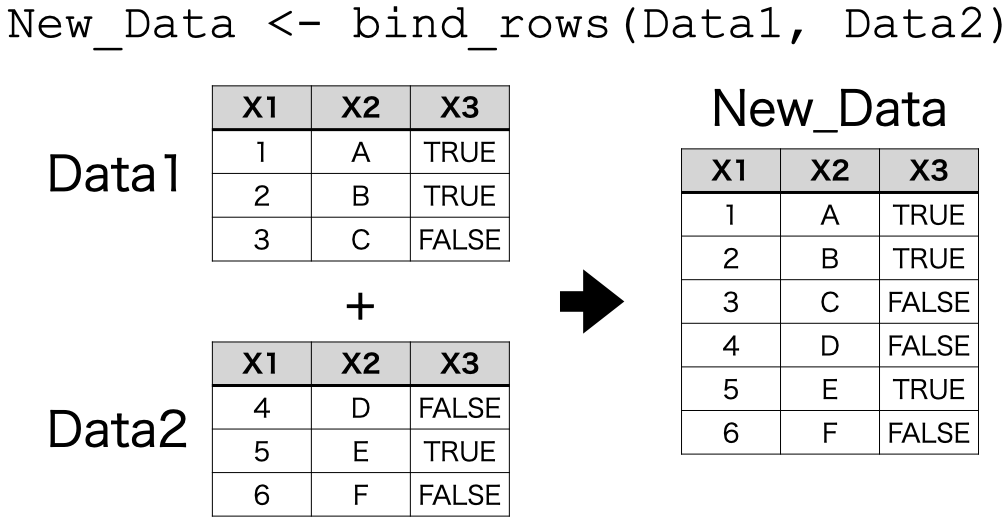
\includegraphics[width=0.75\textwidth,height=\textheight]{./Figs/Handling2/Merge1.png}

}

\caption{\label{fig-handling2_merge_row}行の結合}

\end{figure}

行を結合する際には\texttt{dplyr}パッケージの\texttt{bind\_rows()}関数を使います。この関数の使い方は以下の通りです。

\begin{Shaded}
\begin{Highlighting}[numbers=left,,]
\CommentTok{\# 新しいデータ名ではなく、既にあるデータ名にすると上書きとなる}
\NormalTok{新しいデータ名 }\OtherTok{\textless{}{-}}  \FunctionTok{bind\_rows}\NormalTok{(データ1, データ2, ...)}
\end{Highlighting}
\end{Shaded}

それでは早速実際に使ってみましょう。実習のために、4つのtibbleを作成します
(tibbleでなくデータフレームでも問題ありません)。

\begin{Shaded}
\begin{Highlighting}[numbers=left,,]
\CommentTok{\# tibble()の代わりにdata.frame()も可}
\NormalTok{rbind\_df1 }\OtherTok{\textless{}{-}} \FunctionTok{tibble}\NormalTok{(}\AttributeTok{X1 =} \DecValTok{1}\SpecialCharTok{:}\DecValTok{3}\NormalTok{,}
                    \AttributeTok{X2 =} \FunctionTok{c}\NormalTok{(}\StringTok{"A"}\NormalTok{, }\StringTok{"B"}\NormalTok{, }\StringTok{"C"}\NormalTok{),}
                    \AttributeTok{X3 =} \FunctionTok{c}\NormalTok{(T, T, F)) }\CommentTok{\# TRUEとFALSEはTはFと省略可能}

\NormalTok{rbind\_df2 }\OtherTok{\textless{}{-}} \FunctionTok{tibble}\NormalTok{(}\AttributeTok{X1 =} \DecValTok{4}\SpecialCharTok{:}\DecValTok{6}\NormalTok{,}
                    \AttributeTok{X2 =} \FunctionTok{c}\NormalTok{(}\StringTok{"D"}\NormalTok{, }\StringTok{"E"}\NormalTok{, }\StringTok{"F"}\NormalTok{),}
                    \AttributeTok{X3 =} \FunctionTok{c}\NormalTok{(F, T, F))}

\NormalTok{rbind\_df3 }\OtherTok{\textless{}{-}} \FunctionTok{tibble}\NormalTok{(}\AttributeTok{X1 =} \DecValTok{7}\SpecialCharTok{:}\DecValTok{9}\NormalTok{,}
                    \AttributeTok{X3 =} \FunctionTok{c}\NormalTok{(T, T, T),}
                    \AttributeTok{X2 =} \FunctionTok{c}\NormalTok{(}\StringTok{"G"}\NormalTok{, }\StringTok{"H"}\NormalTok{, }\StringTok{"I"}\NormalTok{))}

\NormalTok{rbind\_df4 }\OtherTok{\textless{}{-}} \FunctionTok{tibble}\NormalTok{(}\AttributeTok{X1 =} \DecValTok{10}\SpecialCharTok{:}\DecValTok{12}\NormalTok{,}
                    \AttributeTok{X2 =} \FunctionTok{c}\NormalTok{(}\StringTok{"J"}\NormalTok{, }\StringTok{"K"}\NormalTok{, }\StringTok{"L"}\NormalTok{),}
                    \AttributeTok{X5 =} \FunctionTok{c}\NormalTok{(}\StringTok{"Song"}\NormalTok{, }\StringTok{"Yanai"}\NormalTok{, }\StringTok{"Hadley"}\NormalTok{))}

\NormalTok{rbind\_df1 }\CommentTok{\# rbind\_df1を出力}
\end{Highlighting}
\end{Shaded}

\begin{verbatim}
# A tibble: 3 x 3
     X1 X2    X3   
  <int> <chr> <lgl>
1     1 A     TRUE 
2     2 B     TRUE 
3     3 C     FALSE
\end{verbatim}

\begin{Shaded}
\begin{Highlighting}[numbers=left,,]
\NormalTok{rbind\_df2 }\CommentTok{\# rbind\_df2を出力}
\end{Highlighting}
\end{Shaded}

\begin{verbatim}
# A tibble: 3 x 3
     X1 X2    X3   
  <int> <chr> <lgl>
1     4 D     FALSE
2     5 E     TRUE 
3     6 F     FALSE
\end{verbatim}

\begin{Shaded}
\begin{Highlighting}[numbers=left,,]
\NormalTok{rbind\_df3 }\CommentTok{\# rbind\_df3を出力}
\end{Highlighting}
\end{Shaded}

\begin{verbatim}
# A tibble: 3 x 3
     X1 X3    X2   
  <int> <lgl> <chr>
1     7 TRUE  G    
2     8 TRUE  H    
3     9 TRUE  I    
\end{verbatim}

\begin{Shaded}
\begin{Highlighting}[numbers=left,,]
\NormalTok{rbind\_df4 }\CommentTok{\# rbind\_df4を出力}
\end{Highlighting}
\end{Shaded}

\begin{verbatim}
# A tibble: 3 x 3
     X1 X2    X5    
  <int> <chr> <chr> 
1    10 J     Song  
2    11 K     Yanai 
3    12 L     Hadley
\end{verbatim}

まずは、\texttt{rbind\_df1}と\texttt{rbind\_df2}を結合してみます。この2つのデータは同じ変数が同じ順番で並んでいますね。

\begin{Shaded}
\begin{Highlighting}[numbers=left,,]
\NormalTok{Binded\_df1 }\OtherTok{\textless{}{-}} \FunctionTok{bind\_rows}\NormalTok{(rbind\_df1, rbind\_df2)}
\NormalTok{Binded\_df1}
\end{Highlighting}
\end{Shaded}

\begin{verbatim}
# A tibble: 6 x 3
     X1 X2    X3   
  <int> <chr> <lgl>
1     1 A     TRUE 
2     2 B     TRUE 
3     3 C     FALSE
4     4 D     FALSE
5     5 E     TRUE 
6     6 F     FALSE
\end{verbatim}

2つのデータが結合されたことが確認できます。それでは\texttt{rbind\_df1}と\texttt{rbind\_df2}、\texttt{rbind\_df3}はどうでしょうか。確かに3つのデータは同じ変数を持ちますが、\texttt{rbind\_df3}は変数の順番が\texttt{X1}、\texttt{X3}、\texttt{X2}になっています。このまま結合するとエラーが出るでしょうか。とりあえず、やってみます。

\begin{Shaded}
\begin{Highlighting}[numbers=left,,]
\NormalTok{Binded\_df2 }\OtherTok{\textless{}{-}} \FunctionTok{bind\_rows}\NormalTok{(rbind\_df1, rbind\_df2, rbind\_df3)}
\NormalTok{Binded\_df2}
\end{Highlighting}
\end{Shaded}

\begin{verbatim}
# A tibble: 9 x 3
     X1 X2    X3   
  <int> <chr> <lgl>
1     1 A     TRUE 
2     2 B     TRUE 
3     3 C     FALSE
4     4 D     FALSE
5     5 E     TRUE 
6     6 F     FALSE
7     7 G     TRUE 
8     8 H     TRUE 
9     9 I     TRUE 
\end{verbatim}

このように変数の順番が異なっても、先に指定したデータの変数順で問題なく結合できました。これまでの作業は\texttt{dplyr}パッケージの\texttt{bind\_rows()}を使わずに、R内蔵関数の\texttt{rbind()}でも同じやり方でできます。\texttt{bind\_rows()}の特徴は、変数名が一致しない場合、つまり今回の例だと\texttt{rbind\_df4}が含まれる場合です。\texttt{rbind\_df1}から\texttt{rbind\_df3}までは順番が違っても\texttt{X1}、\texttt{X2}、\texttt{X3}変数で構成されていました。一方、\texttt{rbind\_dr4}には\texttt{X3}がなく、新たに\texttt{X4}という変数があります。これを\texttt{rbind()}関数で結合するとエラーが出力されます。

\begin{Shaded}
\begin{Highlighting}[numbers=left,,]
\CommentTok{\# rbind()を使う場合}
\FunctionTok{rbind}\NormalTok{(rbind\_df1, rbind\_df2, rbind\_df3, rbind\_df4)}
\end{Highlighting}
\end{Shaded}

\begin{verbatim}
Error in match.names(clabs, names(xi)): names do not match previous names
\end{verbatim}

一方、\texttt{bind\_rows()}はどうでしょうか。

\begin{Shaded}
\begin{Highlighting}[numbers=left,,]
\NormalTok{Binded\_df3 }\OtherTok{\textless{}{-}} \FunctionTok{bind\_rows}\NormalTok{(rbind\_df1, rbind\_df2, rbind\_df3, rbind\_df4)}
\NormalTok{Binded\_df3}
\end{Highlighting}
\end{Shaded}

\begin{verbatim}
# A tibble: 12 x 4
      X1 X2    X3    X5    
   <int> <chr> <lgl> <chr> 
 1     1 A     TRUE  <NA>  
 2     2 B     TRUE  <NA>  
 3     3 C     FALSE <NA>  
 4     4 D     FALSE <NA>  
 5     5 E     TRUE  <NA>  
 6     6 F     FALSE <NA>  
 7     7 G     TRUE  <NA>  
 8     8 H     TRUE  <NA>  
 9     9 I     TRUE  <NA>  
10    10 J     NA    Song  
11    11 K     NA    Yanai 
12    12 L     NA    Hadley
\end{verbatim}

\texttt{X1}から\texttt{X4}まで全ての列が生成され、元のデータにはなかった列に関しては\texttt{NA}で埋められています。

ならば、\texttt{bind\_rows()}の完全勝利かというと、そうとは限りません。自分で架空した複数のデータフレーム、またはtibbleを結合する際、「このデータは全て同じ変数を持っているはず」と事前に分かっているなら\texttt{rbind()}の方が効果的です。なぜなら、変数名が異なる場合、エラーが出力されるからです。\texttt{bind\_rows()}を使うと、コーディングミスなどにより、列名の相違がある場合でも結合してくれてしまうので、分析の結果を歪ませる可能性があります。

\hypertarget{ux5217ux306eux7d50ux5408}{%
\subsection{列の結合}\label{ux5217ux306eux7d50ux5408}}

実はデータ分析においてデータの結合といえば、列の結合が一般的です。これは
図~\ref{fig-handling2_merge_col} のような操作を意味します。

\begin{figure}

{\centering 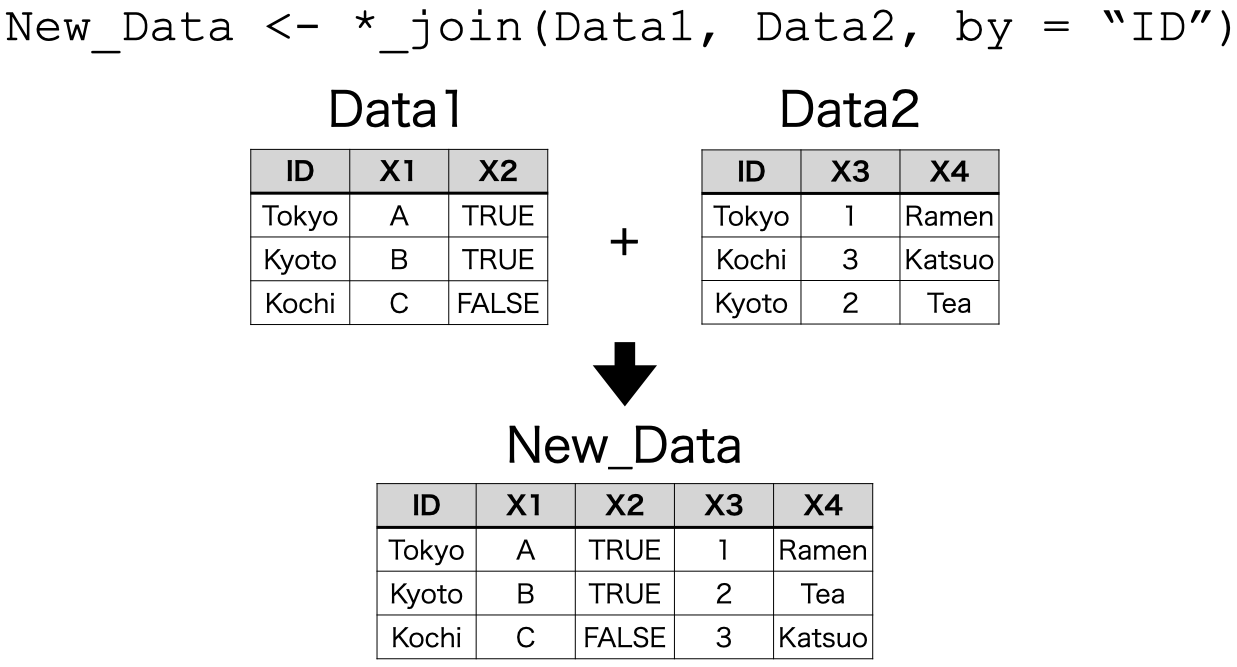
\includegraphics[width=0.75\textwidth,height=\textheight]{./Figs/Handling2/Merge2.png}

}

\caption{\label{fig-handling2_merge_col}列の結合}

\end{figure}

まずは、本章で作成した\texttt{df2}をもう一回作ってみます。

\begin{Shaded}
\begin{Highlighting}[numbers=left,,]
\NormalTok{df2 }\OtherTok{\textless{}{-}}\NormalTok{ df }\SpecialCharTok{\%\textgreater{}\%}
  \FunctionTok{group\_by}\NormalTok{(Pref) }\SpecialCharTok{\%\textgreater{}\%}
  \FunctionTok{summarise}\NormalTok{(}\AttributeTok{Budget\_Mean =} \FunctionTok{mean}\NormalTok{(Budget, }\AttributeTok{na.rm =} \ConstantTok{TRUE}\NormalTok{),}
            \AttributeTok{ScoreN\_Sum  =} \FunctionTok{sum}\NormalTok{(ScoreN, }\AttributeTok{na.rm =} \ConstantTok{TRUE}\NormalTok{),}
            \AttributeTok{Score\_Mean  =} \FunctionTok{mean}\NormalTok{(Score, }\AttributeTok{na.rm =} \ConstantTok{TRUE}\NormalTok{),}
            \AttributeTok{N           =} \FunctionTok{n}\NormalTok{(),}
            \AttributeTok{.groups     =} \StringTok{"drop"}\NormalTok{)}

\NormalTok{df2}
\end{Highlighting}
\end{Shaded}

\begin{verbatim}
# A tibble: 9 x 5
  Pref     Budget_Mean ScoreN_Sum Score_Mean     N
  <chr>          <dbl>      <dbl>      <dbl> <int>
1 京都府         1399.        216       3.68   414
2 兵庫県         1197.        230       3.54   591
3 千葉県         1124.        259       3.72  1000
4 和歌山県       1252          83       3.97   140
5 埼玉県         1147.        278       3.64  1000
6 大阪府         1203.        516       3.77  1000
7 奈良県         1169.         45       3.85   147
8 東京都         1283.       1165       3.67  1000
9 神奈川県       1239.        587       3.53  1000
\end{verbatim}

ラーメン屋の店舗ですが、たしかにデータには埼玉、東京、大阪などは1000店舗しか入っておりません。実はもっと多いですが、ぐるなびAPIの仕様上、最大1000店舗しか情報取得が出来ないからです。ここに実際の店舗数が入っている新しいデータセット、\href{Data/Ramen2.csv}{Ramen2.csv}があります。これを読み込み、\texttt{df3}という名で格納しましょう。

\begin{Shaded}
\begin{Highlighting}[numbers=left,,]
\NormalTok{df3 }\OtherTok{\textless{}{-}} \FunctionTok{read\_csv}\NormalTok{(}\StringTok{"Data/Ramen2.csv"}\NormalTok{)}
\end{Highlighting}
\end{Shaded}

\begin{verbatim}
Rows: 47 Columns: 15
-- Column specification --------------------------------------------------------
Delimiter: ","
chr  (1): Pref
dbl (12): RamenN, Turnout, LDP, CDP, DPFP, Komei, JIP, JCP, SDP, Reiwa, NHK,...

i Use `spec()` to retrieve the full column specification for this data.
i Specify the column types or set `show_col_types = FALSE` to quiet this message.
\end{verbatim}

\begin{Shaded}
\begin{Highlighting}[numbers=left,,]
\NormalTok{df3}
\end{Highlighting}
\end{Shaded}

\begin{verbatim}
# A tibble: 47 x 15
   Pref      Pop   Area RamenN Turnout   LDP   CDP  DPFP Komei   JIP   JCP   SDP
   <chr>   <dbl>  <dbl>  <dbl>   <dbl> <dbl> <dbl> <dbl> <dbl> <dbl> <dbl> <dbl>
 1 北海道 5.38e6 83424.   1454    53.8  32.3  20.8  6.65 11.7   7.78 11.6   1.31
 2 青森県 1.31e6  9646.    336    42.9  39.8  22.0  7.24 11.3   3.4   8.31  2.36
 3 岩手県 1.28e6 15275.    285    56.5  35.5  17.8 12.5   8.22  4.36 10.4   3.83
 4 宮城県 2.33e6  7282.    557    51.2  39.6  17.8  9.02 11.1   4.6   7.89  2.1 
 5 秋田県 1.02e6 11638.    301    56.3  44.5  13.5  8.64 10.6   4.48  8.09  3.77
 6 山形県 1.12e6  9323.    512    60.7  45.2  14.9  7.37  9.87  4.28  6.51  5.08
 7 福島県 1.91e6 13784.    550    52.4  38.2  13.6 12.1  12.8   5.31  7.99  3.01
 8 茨城県 2.92e6  6097.    663    45.0  39.3  15.2  7.15 15.1   6.73  7.73  1.46
 9 栃木県 1.97e6  6408.    595    44.1  40.3  18.9  9.94 12.8   4.9   5.04  1.03
10 群馬県 1.97e6  6362.    488    48.2  40.6  16.4  9.76 12.4   4.67  7.58  1.87
# ... with 37 more rows, and 3 more variables: Reiwa <dbl>, NHK <dbl>,
#   HRP <dbl>
\end{verbatim}

\hypertarget{tbl-handling2_dataset}{}
\begin{table}
\caption{\label{tbl-handling2_dataset}Ramen2.csvの詳細 }

\centering
\begin{tabular}{l|l}
\hline
\multicolumn{1}{c}{変数名} & \multicolumn{1}{c}{説明}\\
\hline
`Pref` & 都道府県名\\
\hline
`Pop` & 日本人人口 (2015年国勢調査)\\
\hline
`Area` & 面積 (2015年国勢調査)\\
\hline
`RamenN` & ぐるなびに登録されたラーメン屋の店舗数\\
\hline
`Turnout` & 2019年参院選: 投票率 (比例)\\
\hline
`LDP` & 2019年参院選: 自民党の得票率 (比例)\\
\hline
`CDP` & 2019年参院選: 立憲民主党の得票率 (比例)\\
\hline
`DPFP` & 2019年参院選: 国民民主党の得票率 (比例)\\
\hline
`Komei` & 2019年参院選: 公明党の得票率 (比例)\\
\hline
`JIP` & 2019年参院選: 日本維新の会の得票率 (比例)\\
\hline
`JCP` & 2019年参院選: 日本共産党の得票率 (比例)\\
\hline
`SDP` & 2019年参院選: 社会民主党の得票率 (比例)\\
\hline
`Reiwa` & 2019年参院選: れいわ新選組の得票率 (比例)\\
\hline
`NHK` & 2019年参院選: NHKから国民を守る党の得票率 (比例)\\
\hline
`HRP` & 2019年参院選: 幸福実現党の得票率 (比例)\\
\hline
\end{tabular}
\end{table}

本データは都道府県ごとの人口、面積、ぐるなびに登録されたラーメン屋の店舗数、2019年参議院議員通常選挙の結果が格納されています。人口と面積は2015年国勢調査、ぐるなびの情報は2020年6月時点での情報です。

\texttt{df2}にデータ上の店舗数ではなく、実際の店舗数を新しい列として追加したい場合はどうすれば良いでしょうか。簡単な方法としては\texttt{df3}から情報を取得し、それを自分で入れる方法です。

\begin{Shaded}
\begin{Highlighting}[numbers=left,,]
\NormalTok{df3 }\SpecialCharTok{\%\textgreater{}\%}
  \CommentTok{\# df2のPrefベクトルの要素と一致するものに絞る}
  \FunctionTok{filter}\NormalTok{(Pref }\SpecialCharTok{\%in\%}\NormalTok{ df2}\SpecialCharTok{$}\NormalTok{Pref) }\SpecialCharTok{\%\textgreater{}\%}
  \CommentTok{\# 都道府県名とラーメン屋の店舗数のみ抽出}
  \FunctionTok{select}\NormalTok{(Pref, RamenN)}
\end{Highlighting}
\end{Shaded}

\begin{verbatim}
# A tibble: 9 x 2
  Pref     RamenN
  <chr>     <dbl>
1 埼玉県     1106
2 千葉県     1098
3 東京都     3220
4 神奈川県   1254
5 京都府      415
6 大阪府     1325
7 兵庫県      591
8 奈良県      147
9 和歌山県    140
\end{verbatim}

そして、この情報を\texttt{df2\$RamenN\ \textless{}-\ c(415,\ 1106,\ 1254,\ ...)}のように追加すればいいですね。

しかし、このような方法は非効率的です。そもそも\texttt{df3}から得られた結果の順番と\texttt{df2}の順番も一致しないので、一々対照しながらベクトルを作ることになります。ここで登場する関数が\texttt{dplyr}の\texttt{*\_join()}関数群です。この関数群には4つの関数が含まれており、以下のような使い方になります。

\begin{Shaded}
\begin{Highlighting}[numbers=left,,]
\CommentTok{\# 新しいデータ名ではなく、データ1またはデータ2の名前に格納すると上書きとなる}

\CommentTok{\# 1. データ1を基準に結合}
\NormalTok{新しいデータ名 }\OtherTok{\textless{}{-}}  \FunctionTok{left\_join}\NormalTok{(データ1, データ2, }\AttributeTok{by =} \StringTok{"共通変数名"}\NormalTok{)}

\CommentTok{\# 2. データ2を基準に結合}
\NormalTok{新しいデータ名 }\OtherTok{\textless{}{-}} \FunctionTok{right\_join}\NormalTok{(データ1, データ2, }\AttributeTok{by =} \StringTok{"共通変数名"}\NormalTok{)}

\CommentTok{\# 3. データ1とデータ2両方に共通するケースのみ結合}
\NormalTok{新しいデータ名 }\OtherTok{\textless{}{-}} \FunctionTok{inner\_join}\NormalTok{(データ1, データ2, }\AttributeTok{by =} \StringTok{"共通変数名"}\NormalTok{)}

\CommentTok{\# 4. データ1とデータ2、どれかに存在するケースを結合}
\NormalTok{新しいデータ名 }\OtherTok{\textless{}{-}}  \FunctionTok{full\_join}\NormalTok{(データ1, データ2, }\AttributeTok{by =} \StringTok{"共通変数名"}\NormalTok{)}
\end{Highlighting}
\end{Shaded}

4つの関数の違いについて説明する前に、\texttt{by}引数について話したいと思います。これは主にキー
(key)変数と呼ばれる変数で、それぞれのデータに同じ名前の変数がある必要があります。\texttt{df2}と\texttt{df3}だとそれが\texttt{Pref}変数です。どの\texttt{*\_join()}関数でも、\texttt{Pref}の値が同じもの同士を結合することになります。

データのキー変数名が異なる場合もあります。たとえば、データ1の都道府県名は\texttt{Pref}という列に、データ2の都道府県名は\texttt{Prefecture}という列になっている場合、\texttt{by\ =\ "Pref"}でなく、\texttt{by\ =\ c("データ1のキー変数名"\ =\ "データ2のキー変数名")}、つまり、\texttt{by\ =\ c("Pref"\ =\ "Prefecture")}と指定します。

それでは、\texttt{df3}から都道府県名とラーメン屋の店舗数だけ抽出し、\texttt{df4}として格納しておきます。

\begin{Shaded}
\begin{Highlighting}[numbers=left,,]
\NormalTok{df4 }\OtherTok{\textless{}{-}}\NormalTok{ df3 }\SpecialCharTok{\%\textgreater{}\%}
  \FunctionTok{select}\NormalTok{(Pref, RamenN)}

\NormalTok{df4}
\end{Highlighting}
\end{Shaded}

\begin{verbatim}
# A tibble: 47 x 2
   Pref   RamenN
   <chr>   <dbl>
 1 北海道   1454
 2 青森県    336
 3 岩手県    285
 4 宮城県    557
 5 秋田県    301
 6 山形県    512
 7 福島県    550
 8 茨城県    663
 9 栃木県    595
10 群馬県    488
# ... with 37 more rows
\end{verbatim}

これから共通変数名の値をキー
(key)と呼びます。今回の例だと\texttt{Pref}が\texttt{df2}と\texttt{df4}のキー変数であり、その値である\texttt{"東京都"}、\texttt{"北海道"}などがキーです。

まずは、\texttt{inner\_join()}の仕組みについて考えます。これは\texttt{df2}と\texttt{df4}に共通するキーを持つケースのみ結合する関数です。\texttt{df4}には\texttt{"北海道"}というキーがありますが、\texttt{df2}にはありません。したがって、キーが\texttt{"北海道"}のケースは結合から除外されます。これをイメージにしたものが
図~\ref{fig-handling2_merge_inner} です\footnote{これらの図は
  \citet{Grolemund_Wickham:2016} を参考にしました。}。それぞれ3
\(\times\) 2
(3行2列)のデータですが、キーが一致するケースは2つしかないため、結合後のデータは3
\(\times\) 2となります。

\begin{figure}

{\centering 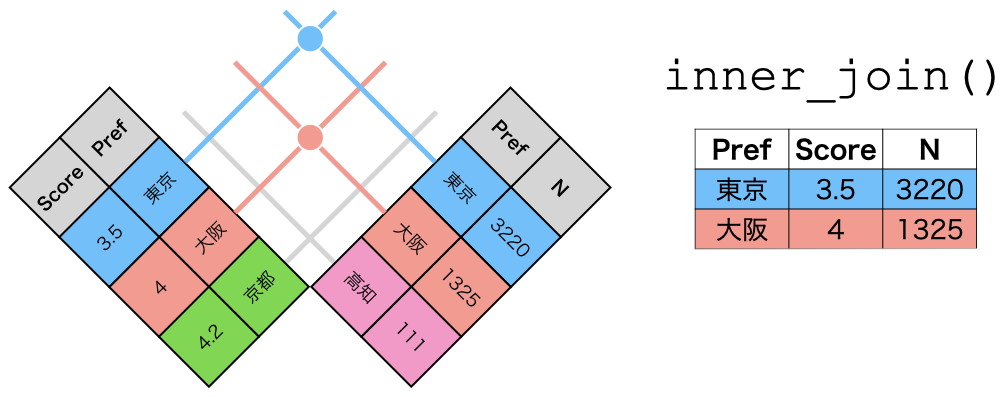
\includegraphics[width=0.75\textwidth,height=\textheight]{./Figs/Handling2/Merge_Inner.png}

}

\caption{\label{fig-handling2_merge_inner}\texttt{inner\_join()}の仕組み}

\end{figure}

実際にやってみましょう。

\begin{Shaded}
\begin{Highlighting}[numbers=left,,]
\FunctionTok{inner\_join}\NormalTok{(df2, df4, }\AttributeTok{by =} \StringTok{"Pref"}\NormalTok{)}
\end{Highlighting}
\end{Shaded}

\begin{verbatim}
# A tibble: 9 x 6
  Pref     Budget_Mean ScoreN_Sum Score_Mean     N RamenN
  <chr>          <dbl>      <dbl>      <dbl> <int>  <dbl>
1 京都府         1399.        216       3.68   414    415
2 兵庫県         1197.        230       3.54   591    591
3 千葉県         1124.        259       3.72  1000   1098
4 和歌山県       1252          83       3.97   140    140
5 埼玉県         1147.        278       3.64  1000   1106
6 大阪府         1203.        516       3.77  1000   1325
7 奈良県         1169.         45       3.85   147    147
8 東京都         1283.       1165       3.67  1000   3220
9 神奈川県       1239.        587       3.53  1000   1254
\end{verbatim}

共通するキーは9つのみであり、結果として返されたデータの大きさも9
\(\times\)
6です。\texttt{df2}に足された\texttt{df4}は2列のデータですが、キー変数である\texttt{Pref}は共通するため、1列のみ足されました。キー変数を両方残す場合は\texttt{keep\ =\ TRUE}引数を追加してください。

一方、\texttt{full\_join()}は、すべてのキーに対して結合を行います (
図~\ref{fig-handling2_merge_full}
)。たとえば、\texttt{df2}には\texttt{"北海道"}というキーがありません。それでも新しく出来上がるデータには北海道の列が追加されます。ただし、道内店舗の平均予算、口コミ数などの情報はないため、欠損値が代入されます。

\begin{figure}

{\centering 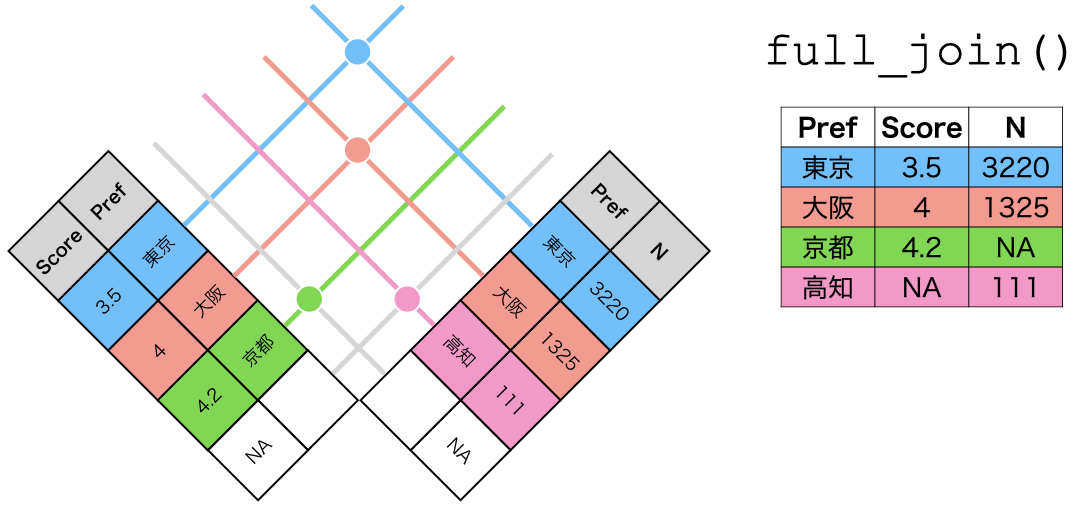
\includegraphics[width=0.75\textwidth,height=\textheight]{./Figs/Handling2/Merge_Full.png}

}

\caption{\label{fig-handling2_merge_full}\texttt{full\_join()}の仕組み}

\end{figure}

それでは実際、結果を確認してみましょう。今回は結合後、\texttt{RamenN}が大きい順で出力します。

\begin{Shaded}
\begin{Highlighting}[numbers=left,,]
\FunctionTok{full\_join}\NormalTok{(df2, df4, }\AttributeTok{by =} \StringTok{"Pref"}\NormalTok{) }\SpecialCharTok{\%\textgreater{}\%}
  \FunctionTok{arrange}\NormalTok{(}\FunctionTok{desc}\NormalTok{(RamenN)) }\CommentTok{\# ぐるなびに登録された店舗の多い都道府県から出力}
\end{Highlighting}
\end{Shaded}

\begin{verbatim}
# A tibble: 47 x 6
   Pref     Budget_Mean ScoreN_Sum Score_Mean     N RamenN
   <chr>          <dbl>      <dbl>      <dbl> <int>  <dbl>
 1 東京都         1283.       1165       3.67  1000   3220
 2 北海道           NA          NA      NA       NA   1454
 3 大阪府         1203.        516       3.77  1000   1325
 4 愛知県           NA          NA      NA       NA   1255
 5 神奈川県       1239.        587       3.53  1000   1254
 6 埼玉県         1147.        278       3.64  1000   1106
 7 千葉県         1124.        259       3.72  1000   1098
 8 福岡県           NA          NA      NA       NA    985
 9 新潟県           NA          NA      NA       NA    705
10 静岡県           NA          NA      NA       NA    679
# ... with 37 more rows
\end{verbatim}

\texttt{df2}にはなかった北海道や愛知県などの行ができました。そして、\texttt{df2}にはない情報はすべて欠損値
(\texttt{NA})となりました。

続いて、\texttt{left\_join()}ですが、これは先に指定したデータに存在するキーのみで結合を行います
( 図~\ref{fig-handling2_merge_left}
)。今回は\texttt{df2}が先に指定されていますが、\texttt{df2}のキーは\texttt{df4}のキーの部分集合であるため、\texttt{inner\_join()}と同じ結果が得られます。

\begin{figure}

{\centering 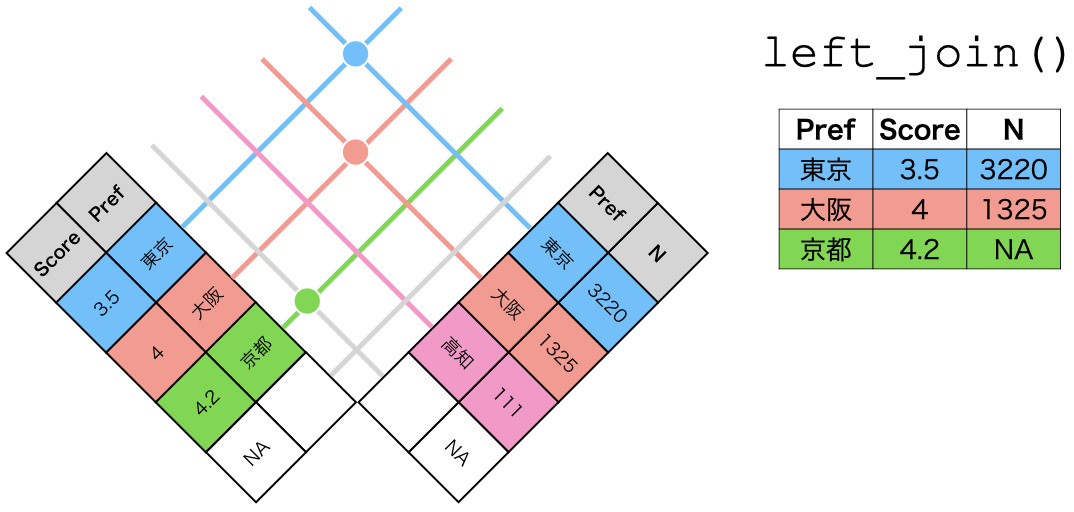
\includegraphics[width=0.75\textwidth,height=\textheight]{./Figs/Handling2/Merge_Left.png}

}

\caption{\label{fig-handling2_merge_left}\texttt{left\_join()}の仕組み}

\end{figure}

一方、\texttt{right\_join()}は\texttt{left\_join()}と逆の関数であり、後に指定したデータに存在するキーを基準に結合を行います
( 図~\ref{fig-handling2_merge_right}
)。後に指定された\texttt{df4}のキーは\texttt{df2}のキーを完全に含むので、\texttt{full\_join()}と同じ結果が得られます。

\begin{figure}

{\centering 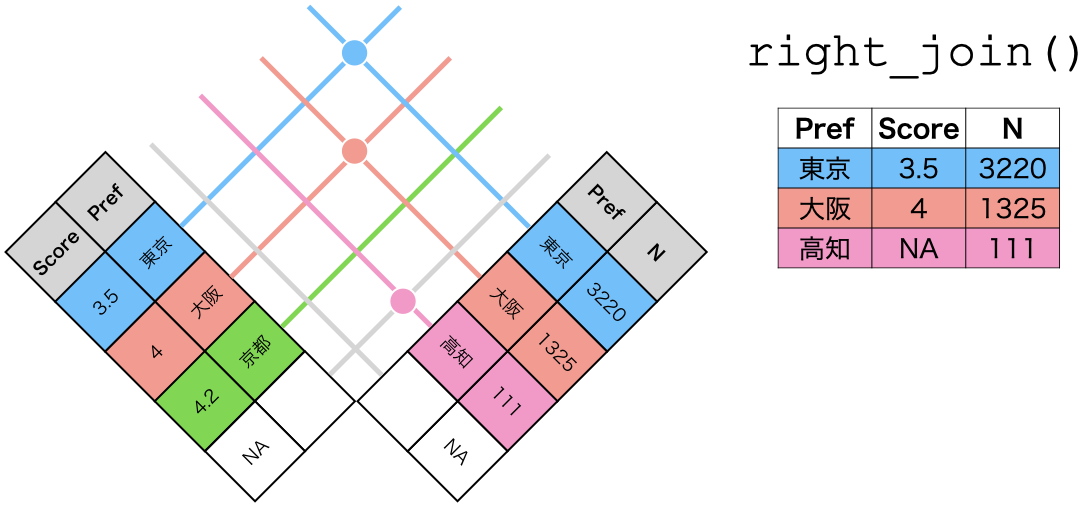
\includegraphics[width=0.75\textwidth,height=\textheight]{./Figs/Handling2/Merge_Right.png}

}

\caption{\label{fig-handling2_merge_right}\texttt{right}\_join()`の仕組み}

\end{figure}

これからは\texttt{df2}と\texttt{df4}を結合することになりますが、この2つのtibbleの大きさが異なります。\texttt{df2}は9つの都府県のみであるに対し、\texttt{df4}は47都道府県全てのデータが入っているからです。

ここまではキー変数が一つである場合についてのみ考えましたが、複数のキー変数が必要な場合もあります。たとえば、市区町村の人口・面積データと市区町村の投票率データを結合するとします。各自治体に与えられている「\href{https://www.soumu.go.jp/denshijiti/code.html}{全国地方公共団体コード}」が両データに含まれている場合は、このコードをキー変数として使えば問題ありませんが、市区町村名をキー変数として使わざる得ないケースもあるでしょう。しかし、キー変数が複数ある場合もあります。たとえば、府中市は東京都と広島県にありますし、太子町は大阪府と兵庫県にあります。この場合、市区町村名のみでケースをマッチングすると、重複されてマッチングされる恐れがあります。この場合はキー変数を増やすことで対処できます。たとえば、同じ都道府県なら同じ市区町村は存在しないでしょう\footnote{行政区も含むなら多くの政令指定都市にある「南区」とか「北区」が重複しますが、ここでは考えないことにしましょう。}。キー変数を複数指定する方法は簡単です。たとえば、市区町村名変数が\texttt{Munip}、都道府県名変数が\texttt{Pref}なら\texttt{by\ =\ c("Munip",\ "Pref")}と指定するだけです。

最後に、キー変数以外の変数名が重複する場合について考えましょう。これはパネルデータを結合する時によく直面する問題です。同じ回答者に2回の調査を行った場合、回答者のIDでデータを結合することになります。ただし、それぞれのデータにおいて回答者の性別に関する変数が\texttt{F1}という名前の場合、どうなるでしょうか。同じデータの同じ名前の変数が複数あると、非常に扱いにくくなります。実際の結果を見てみましょう。

\begin{Shaded}
\begin{Highlighting}[numbers=left,,]
\NormalTok{Wave1\_df }\OtherTok{\textless{}{-}} \FunctionTok{tibble}\NormalTok{(}\AttributeTok{ID =} \FunctionTok{c}\NormalTok{(}\DecValTok{1}\NormalTok{, }\DecValTok{2}\NormalTok{, }\DecValTok{3}\NormalTok{, }\DecValTok{4}\NormalTok{, }\DecValTok{5}\NormalTok{),}
                   \AttributeTok{F1 =} \FunctionTok{c}\NormalTok{(}\DecValTok{1}\NormalTok{, }\DecValTok{1}\NormalTok{, }\DecValTok{0}\NormalTok{, }\DecValTok{0}\NormalTok{, }\DecValTok{1}\NormalTok{),}
                   \AttributeTok{F2 =} \FunctionTok{c}\NormalTok{(}\DecValTok{18}\NormalTok{, }\DecValTok{77}\NormalTok{, }\DecValTok{37}\NormalTok{, }\DecValTok{50}\NormalTok{, }\DecValTok{41}\NormalTok{),}
                   \AttributeTok{Q1 =} \FunctionTok{c}\NormalTok{(}\DecValTok{1}\NormalTok{, }\DecValTok{5}\NormalTok{, }\DecValTok{2}\NormalTok{, }\DecValTok{2}\NormalTok{, }\DecValTok{3}\NormalTok{))}

\NormalTok{Wave2\_df }\OtherTok{\textless{}{-}} \FunctionTok{tibble}\NormalTok{(}\AttributeTok{ID =} \FunctionTok{c}\NormalTok{(}\DecValTok{1}\NormalTok{, }\DecValTok{3}\NormalTok{, }\DecValTok{4}\NormalTok{, }\DecValTok{6}\NormalTok{, }\DecValTok{7}\NormalTok{),}
                   \AttributeTok{F1 =} \FunctionTok{c}\NormalTok{(}\DecValTok{1}\NormalTok{, }\DecValTok{0}\NormalTok{, }\DecValTok{0}\NormalTok{, }\DecValTok{0}\NormalTok{, }\DecValTok{1}\NormalTok{),}
                   \AttributeTok{F2 =} \FunctionTok{c}\NormalTok{(}\DecValTok{18}\NormalTok{, }\DecValTok{37}\NormalTok{, }\DecValTok{50}\NormalTok{, }\DecValTok{20}\NormalTok{, }\DecValTok{62}\NormalTok{),}
                   \AttributeTok{Q1 =} \FunctionTok{c}\NormalTok{(}\DecValTok{1}\NormalTok{, }\DecValTok{2}\NormalTok{, }\DecValTok{2}\NormalTok{, }\DecValTok{5}\NormalTok{, }\DecValTok{4}\NormalTok{))}

\FunctionTok{full\_join}\NormalTok{(Wave1\_df, Wave2\_df, }\AttributeTok{by =} \StringTok{"ID"}\NormalTok{)}
\end{Highlighting}
\end{Shaded}

\begin{verbatim}
# A tibble: 7 x 7
     ID  F1.x  F2.x  Q1.x  F1.y  F2.y  Q1.y
  <dbl> <dbl> <dbl> <dbl> <dbl> <dbl> <dbl>
1     1     1    18     1     1    18     1
2     2     1    77     5    NA    NA    NA
3     3     0    37     2     0    37     2
4     4     0    50     2     0    50     2
5     5     1    41     3    NA    NA    NA
6     6    NA    NA    NA     0    20     5
7     7    NA    NA    NA     1    62     4
\end{verbatim}

それぞれの変数名の後に\texttt{.x}と\texttt{.y}が付きます。この接尾辞
(suffix)は\texttt{suffix}引数を指定することで、分析側からカスタマイズ可能です。たとえば、接尾辞を\texttt{\_W1}、\texttt{\_W2}にしたい場合は

\begin{Shaded}
\begin{Highlighting}[numbers=left,,]
\FunctionTok{full\_join}\NormalTok{(Wave1\_df, Wave2\_df, }\AttributeTok{by =} \StringTok{"ID"}\NormalTok{, }\AttributeTok{suffix =} \FunctionTok{c}\NormalTok{(}\StringTok{"\_W1"}\NormalTok{, }\StringTok{"\_W2"}\NormalTok{))}
\end{Highlighting}
\end{Shaded}

\begin{verbatim}
# A tibble: 7 x 7
     ID F1_W1 F2_W1 Q1_W1 F1_W2 F2_W2 Q1_W2
  <dbl> <dbl> <dbl> <dbl> <dbl> <dbl> <dbl>
1     1     1    18     1     1    18     1
2     2     1    77     5    NA    NA    NA
3     3     0    37     2     0    37     2
4     4     0    50     2     0    50     2
5     5     1    41     3    NA    NA    NA
6     6    NA    NA    NA     0    20     5
7     7    NA    NA    NA     1    62     4
\end{verbatim}

のように、データ1とデータ2それぞれの接尾辞を指定するだけです。

\hypertarget{sec-factor}{%
\chapter{データハンドリング {[}factor型{]}}\label{sec-factor}}

\hypertarget{ux540dux76eeux5909ux6570ux3092ux542bux3080ux30b0ux30e9ux30d5ux3092ux4f5cux6210ux3059ux308bux969bux306eux6ce8ux610fux70b9}{%
\section{名目変数を含むグラフを作成する際の注意点}\label{ux540dux76eeux5909ux6570ux3092ux542bux3080ux30b0ux30e9ux30d5ux3092ux4f5cux6210ux3059ux308bux969bux306eux6ce8ux610fux70b9}}

ここからは楽しい可視化、つまりグラフの作成について解説します。ただし、その前に、名目変数の扱いと簡潔データ構造について話したいと思います。本章では名目変数の扱いについて解説し、次章は簡潔データ構造について解説します。

横軸、または縦軸が気温、成績、身長のような連続変数ではなく、都道府県や国、企業のような名目変数になる場合があります。たとえば、棒グラフの横軸は
図~\ref{fig-factor1} のように、一般的に名目変数になる場合が多いです。

\begin{figure}

{\centering 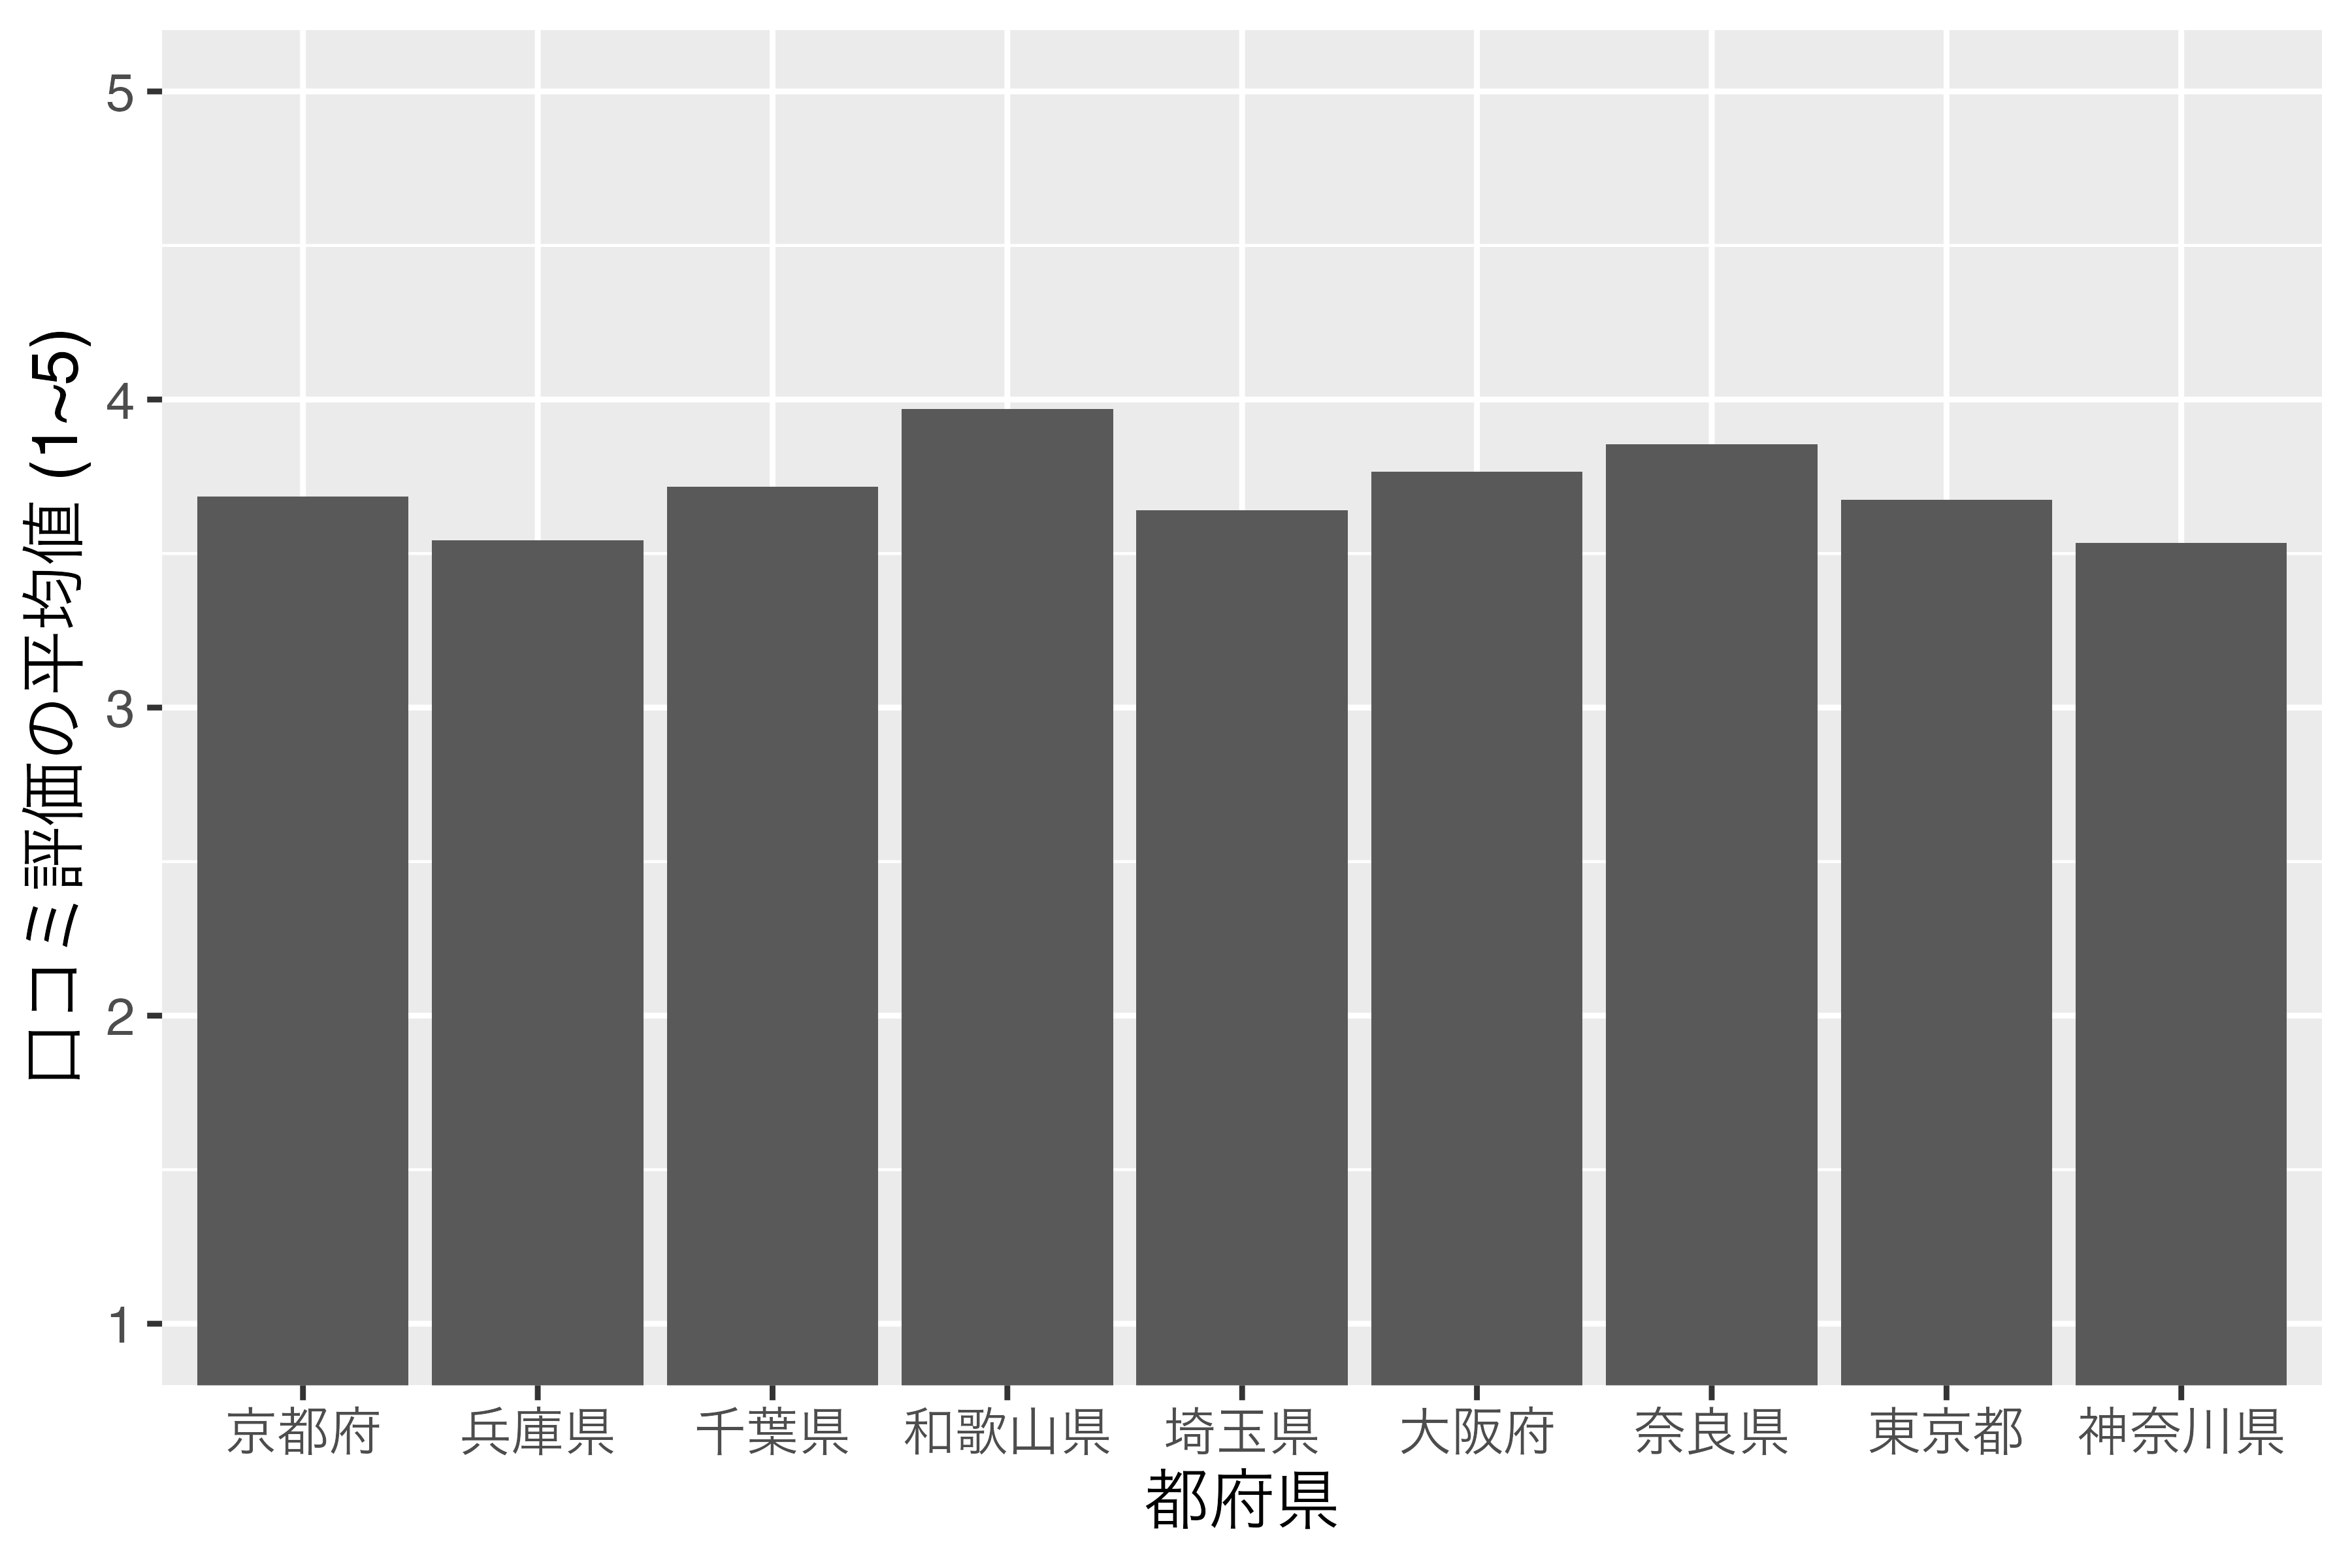
\includegraphics{./factor_files/figure-pdf/fig-factor1-1.png}

}

\caption{\label{fig-factor1}横軸が名目変数の棒グラフ}

\end{figure}

ここでは横軸の順番に注目してください。京都府、埼玉県、神奈川県、\ldots の順番になっていますね。「この順番で大満足だよ!」という方がいるかも知れませんが、そうでない方もおおいでしょう。普通考えられるものとしては、都道府県コードの順か、縦軸が高い順
(低い順)でしょう。都道府県コードの順だと、埼玉県、千葉県、東京都、神奈川県、京都府、大阪府、兵庫県、奈良県、和歌山県の順番になります。または、縦軸
(口コミ評価の平均値)が高い順なら和歌山県、奈良県、大阪府、\ldots の順番になります。あるいは50音順も考えられるでしょう。アメリカの場合、州を並べる際、アルファベット順で並べます。

自分でこの順番をコントロールするには可視化の前の段階、つまりデータハンドリングの段階で順番を決めなくてはなりません。これを決めておかない場合、Rが勝手に順番を指定します。具体的にはロケール
(locale)というパソコン内の空間に文字情報が含まれているわけですが、そこに保存されている文字の順番となります。たとえば、日本語ロケールには「京」が「埼」よりも先に保存されているわけです。

したがって、名目変数がグラフに含まれる場合は、名目変数の表示順番を決める必要があり、そこで必要なのがfactor型です。名目変数がcharacter型の場合、ロケールに保存されている順でソートされますが、factor型の場合、予め指定した順番でソートされます。

たとえば、\href{Data/Ramen.csv}{前章で使用したデータ}を用いて、都道府県ごとの口コミ評価の平均値を計算し、その結果を\texttt{Score\_df}として保存します。

\begin{Shaded}
\begin{Highlighting}[numbers=left,,]
\CommentTok{\# tidyverseパッケージの読み込み}
\FunctionTok{library}\NormalTok{(tidyverse)}
\CommentTok{\# データの読み込み}
\NormalTok{df }\OtherTok{\textless{}{-}} \FunctionTok{read\_csv}\NormalTok{(}\StringTok{"Data/Ramen.csv"}\NormalTok{)}
\end{Highlighting}
\end{Shaded}

\begin{Shaded}
\begin{Highlighting}[numbers=left,,]
\NormalTok{Score\_df }\OtherTok{\textless{}{-}}\NormalTok{ df }\SpecialCharTok{\%\textgreater{}\%}
    \FunctionTok{group\_by}\NormalTok{(Pref) }\SpecialCharTok{\%\textgreater{}\%}
    \FunctionTok{summarise}\NormalTok{(}\AttributeTok{Score   =} \FunctionTok{mean}\NormalTok{(Score, }\AttributeTok{na.rm =} \ConstantTok{TRUE}\NormalTok{),}
              \AttributeTok{.groups =} \StringTok{"drop"}\NormalTok{)}

\NormalTok{Score\_df}
\end{Highlighting}
\end{Shaded}

\begin{verbatim}
# A tibble: 9 x 2
  Pref     Score
  <chr>    <dbl>
1 京都府    3.68
2 兵庫県    3.54
3 千葉県    3.72
4 和歌山県  3.97
5 埼玉県    3.64
6 大阪府    3.77
7 奈良県    3.85
8 東京都    3.67
9 神奈川県  3.53
\end{verbatim}

この時点で勝手にロケール順になります。実際、表示された\texttt{Score\_df}を見ると\texttt{Pref}の下に\texttt{\textless{}chr\textgreater{}}と表記されており\footnote{tibble型でなく、data.frame型の場合、各列のデータ型は表示されませんので、csv形式の読み込みの際は、\texttt{read\_csv()}を使いましょう。}、\texttt{Pref}はcharacter型であることが分かります。これをこのまま棒グラフに出してみましょう。可視化の方法はこれから詳細に解説するので、ここでは結果だけに注目してください。

\begin{Shaded}
\begin{Highlighting}[numbers=left,,]
\NormalTok{Score\_df }\SpecialCharTok{\%\textgreater{}\%}
  \FunctionTok{ggplot}\NormalTok{() }\SpecialCharTok{+}
  \FunctionTok{geom\_bar}\NormalTok{(}\FunctionTok{aes}\NormalTok{(}\AttributeTok{x =}\NormalTok{ Pref, }\AttributeTok{y =}\NormalTok{ Score), }\AttributeTok{stat =} \StringTok{"identity"}\NormalTok{) }\SpecialCharTok{+}
  \FunctionTok{labs}\NormalTok{(}\AttributeTok{x =} \StringTok{"都府県"}\NormalTok{, }\AttributeTok{y =} \StringTok{"口コミ評価の平均値 (1\textasciitilde{}5)"}\NormalTok{) }\SpecialCharTok{+}
  \FunctionTok{theme}\NormalTok{(}\AttributeTok{text =} \FunctionTok{element\_text}\NormalTok{(}\AttributeTok{size =} \DecValTok{12}\NormalTok{))}
\end{Highlighting}
\end{Shaded}

\begin{figure}[H]

{\centering 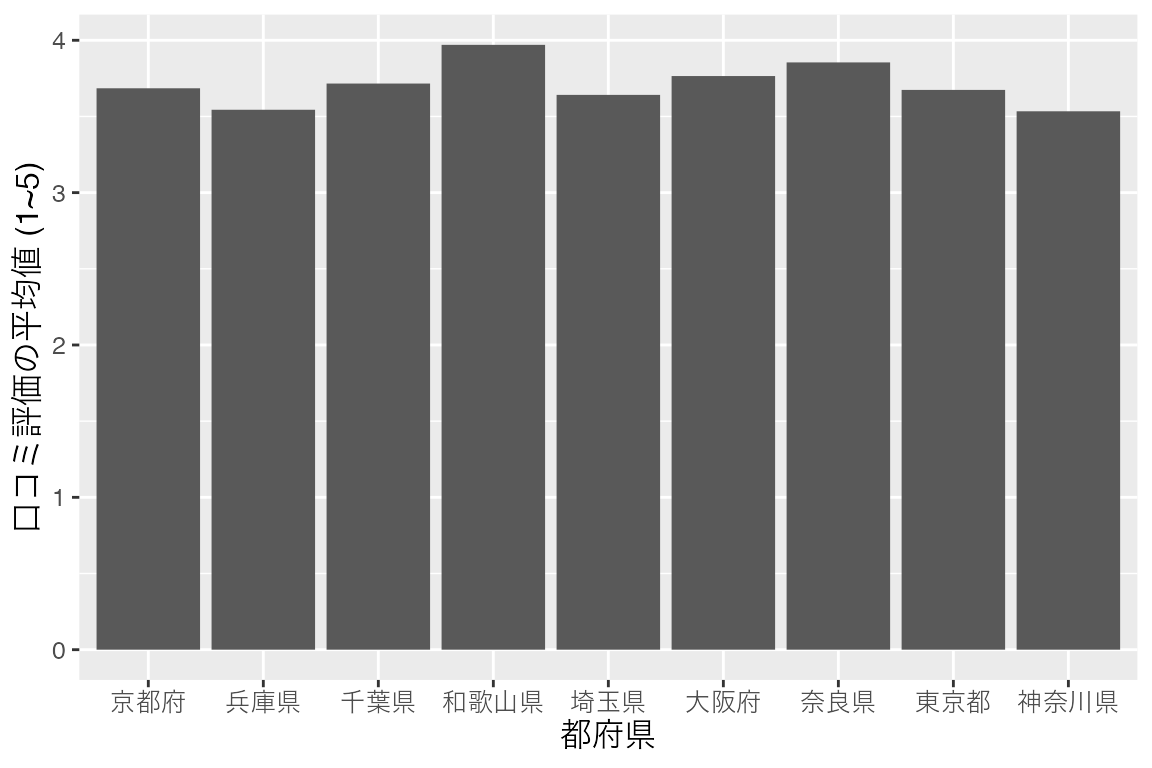
\includegraphics{./factor_files/figure-pdf/fig-factor2-1.png}

}

\caption{\label{fig-factor2}Prefがcharacter型の場合 (1)}

\end{figure}

横軸の順番があまり直感的ではありませんね。それでは、\texttt{Score\_df}を\texttt{Score}が高い順にソートし、\texttt{Score\_df2}で保存してから、もう一回試してみます。

\begin{Shaded}
\begin{Highlighting}[numbers=left,,]
\NormalTok{Score\_df2 }\OtherTok{\textless{}{-}}\NormalTok{ Score\_df }\SpecialCharTok{\%\textgreater{}\%}
  \FunctionTok{arrange}\NormalTok{(}\FunctionTok{desc}\NormalTok{(Score))}

\NormalTok{Score\_df2}
\end{Highlighting}
\end{Shaded}

\begin{verbatim}
# A tibble: 9 x 2
  Pref     Score
  <chr>    <dbl>
1 和歌山県  3.97
2 奈良県    3.85
3 大阪府    3.77
4 千葉県    3.72
5 京都府    3.68
6 東京都    3.67
7 埼玉県    3.64
8 兵庫県    3.54
9 神奈川県  3.53
\end{verbatim}

ここでも\texttt{Pref}はcharacter型ですが、とりあえず、これで図を出してみます。

\begin{Shaded}
\begin{Highlighting}[numbers=left,,]
\NormalTok{Score\_df2 }\SpecialCharTok{\%\textgreater{}\%}
  \FunctionTok{ggplot}\NormalTok{() }\SpecialCharTok{+}
  \FunctionTok{geom\_bar}\NormalTok{(}\FunctionTok{aes}\NormalTok{(}\AttributeTok{x =}\NormalTok{ Pref, }\AttributeTok{y =}\NormalTok{ Score), }\AttributeTok{stat =} \StringTok{"identity"}\NormalTok{) }\SpecialCharTok{+}
  \FunctionTok{labs}\NormalTok{(}\AttributeTok{x =} \StringTok{"都府県"}\NormalTok{, }\AttributeTok{y =} \StringTok{"口コミ評価の平均値 (1\textasciitilde{}5)"}\NormalTok{) }\SpecialCharTok{+}
  \FunctionTok{theme}\NormalTok{(}\AttributeTok{text =} \FunctionTok{element\_text}\NormalTok{(}\AttributeTok{size =} \DecValTok{12}\NormalTok{))}
\end{Highlighting}
\end{Shaded}

\begin{figure}[H]

{\centering 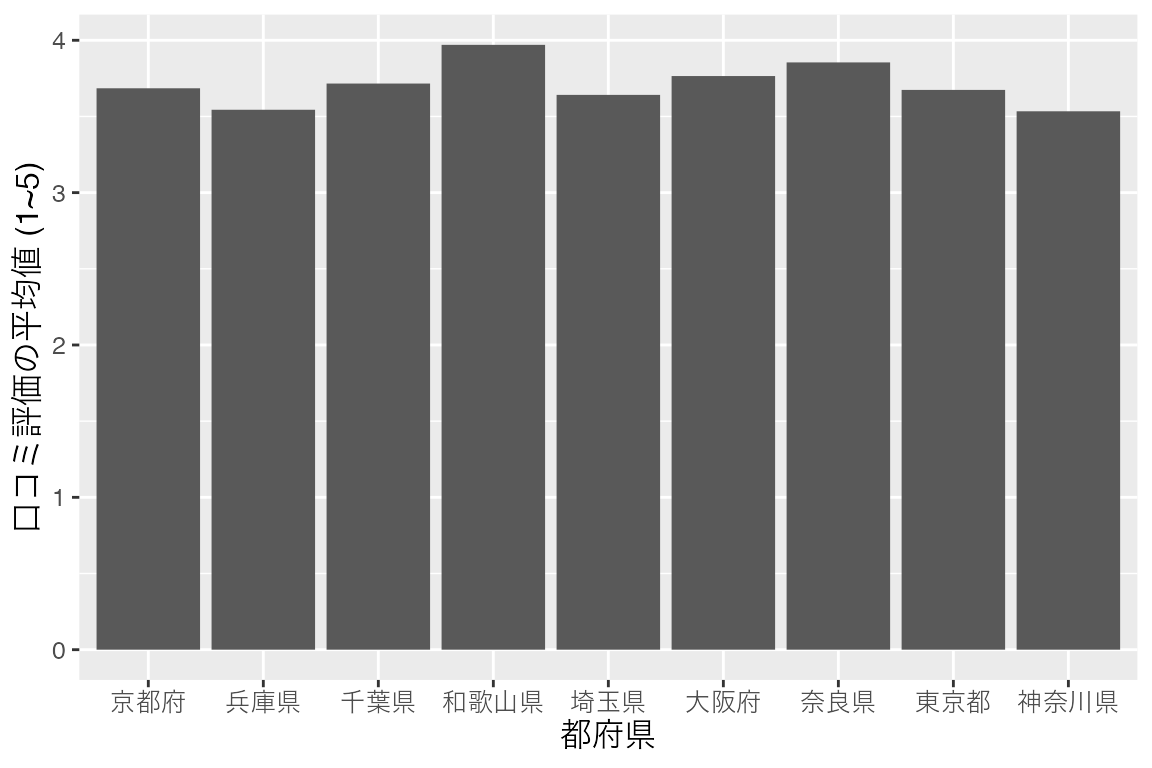
\includegraphics{./factor_files/figure-pdf/fig-factor3-1.png}

}

\caption{\label{fig-factor3}Prefがcharacter型の場合 (2)}

\end{figure}

結果は全く変わっておりません。それでは、\texttt{Score\_df}の\texttt{Pref}列をfactor型に変換し、順番は口コミ評価の平均値が高い順番にしてみましょう。結果は\texttt{Score\_df\_f1}という名で保存します。

\begin{Shaded}
\begin{Highlighting}[numbers=left,,]
\NormalTok{Score\_df\_f1 }\OtherTok{\textless{}{-}}\NormalTok{ Score\_df }\SpecialCharTok{\%\textgreater{}\%}
  \FunctionTok{mutate}\NormalTok{(}\AttributeTok{Pref =} \FunctionTok{factor}\NormalTok{(Pref, }\AttributeTok{levels =} \FunctionTok{c}\NormalTok{(}\StringTok{"和歌山県"}\NormalTok{, }\StringTok{"奈良県"}\NormalTok{, }\StringTok{"大阪府"}\NormalTok{,}
                                        \StringTok{"千葉県"}\NormalTok{, }\StringTok{"京都府"}\NormalTok{, }\StringTok{"東京都"}\NormalTok{,}
                                        \StringTok{"埼玉県"}\NormalTok{, }\StringTok{"兵庫県"}\NormalTok{, }\StringTok{"神奈川県"}\NormalTok{)))}

\NormalTok{Score\_df\_f1}
\end{Highlighting}
\end{Shaded}

\begin{verbatim}
# A tibble: 9 x 2
  Pref     Score
  <fct>    <dbl>
1 京都府    3.68
2 兵庫県    3.54
3 千葉県    3.72
4 和歌山県  3.97
5 埼玉県    3.64
6 大阪府    3.77
7 奈良県    3.85
8 東京都    3.67
9 神奈川県  3.53
\end{verbatim}

表示される順番は\texttt{Score\_df}と\texttt{Score\_df\_f1}も同じですが、\texttt{Pref}のデータ型が\texttt{\textless{}fct\textgreater{}}、つまりfactor型であることが分かります。実際、\texttt{Pref}列だけ抽出した場合、factor型として、和歌山県から神奈川県の順になっていることが確認できます。

\begin{Shaded}
\begin{Highlighting}[numbers=left,,]
\NormalTok{Score\_df\_f1}\SpecialCharTok{$}\NormalTok{Pref}
\end{Highlighting}
\end{Shaded}

\begin{verbatim}
[1] 京都府   兵庫県   千葉県   和歌山県 埼玉県   大阪府   奈良県   東京都  
[9] 神奈川県
9 Levels: 和歌山県 奈良県 大阪府 千葉県 京都府 東京都 埼玉県 ... 神奈川県
\end{verbatim}

この\texttt{Score\_df\_f1}データを使って、 図~\ref{fig-factor2}
と全く同じコードを実行した結果が 図~\ref{fig-factor4} です。

\begin{Shaded}
\begin{Highlighting}[numbers=left,,]
\NormalTok{Score\_df\_f1 }\SpecialCharTok{\%\textgreater{}\%}
  \FunctionTok{ggplot}\NormalTok{() }\SpecialCharTok{+}
  \FunctionTok{geom\_bar}\NormalTok{(}\FunctionTok{aes}\NormalTok{(}\AttributeTok{x =}\NormalTok{ Pref, }\AttributeTok{y =}\NormalTok{ Score), }\AttributeTok{stat =} \StringTok{"identity"}\NormalTok{) }\SpecialCharTok{+}
  \FunctionTok{labs}\NormalTok{(}\AttributeTok{x =} \StringTok{"都府県"}\NormalTok{, }\AttributeTok{y =} \StringTok{"口コミ評価の平均値 (1\textasciitilde{}5)"}\NormalTok{) }\SpecialCharTok{+}
  \FunctionTok{theme}\NormalTok{(}\AttributeTok{text =} \FunctionTok{element\_text}\NormalTok{(}\AttributeTok{size =} \DecValTok{12}\NormalTok{))}
\end{Highlighting}
\end{Shaded}

\begin{figure}[H]

{\centering 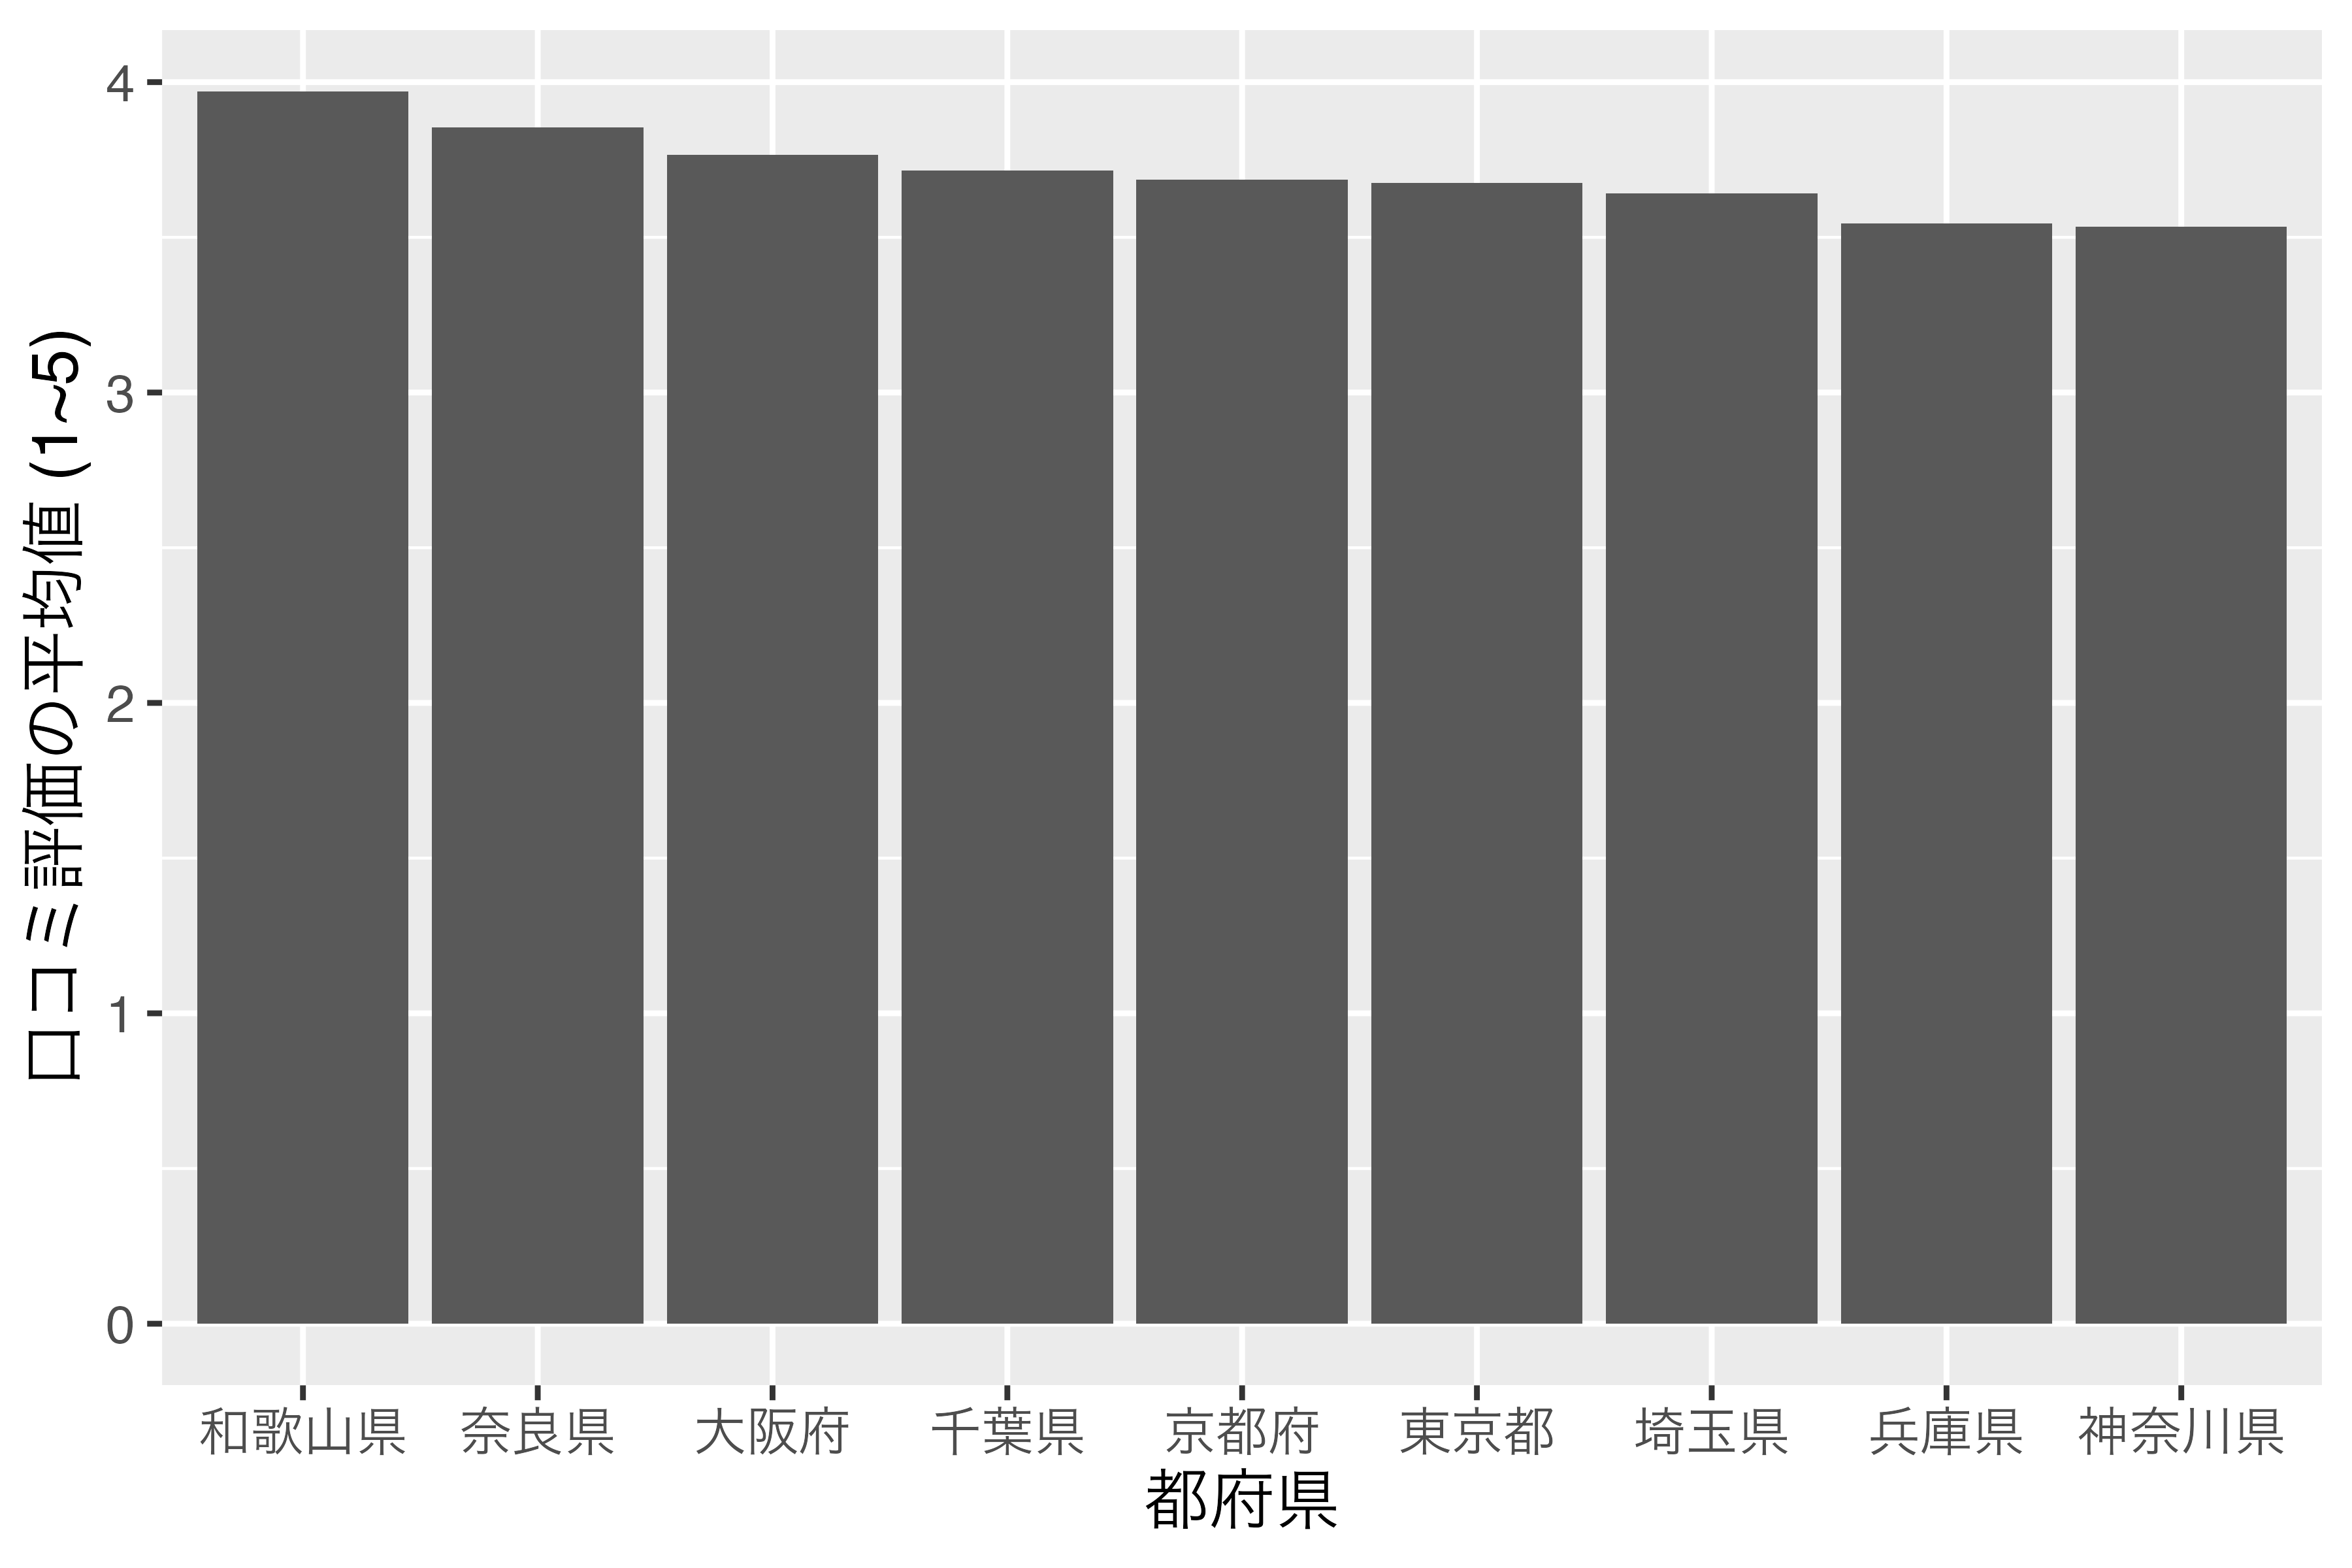
\includegraphics{./factor_files/figure-pdf/fig-factor4-1.png}

}

\caption{\label{fig-factor4}Prefがcharacter型の場合 (3)}

\end{figure}

これまでの話をまとめるの以下の2点が分かります。

\begin{enumerate}
\def\labelenumi{\arabic{enumi}.}
\tightlist
\item
  変数がcharacter型である場合、自動的にロケール順でソートされる。
\item
  変数がfactor型である場合、データ内の順番やロケール順と関係なく、指定されたレベル
  (水準)の順でソートされる。
\end{enumerate}

とくに2番目の点についてですが、これは必ずしも順序付きfactorである必要はありません。順序付きfactor型でなくても、\texttt{factor()}内で指定した順にソートされます。むろん、順序付きfactor型なら指定された順序でソートされます。

これからはfactor型変換の際に便利な関数をいくつか紹介しますが、その前に数値として表現された名目変数について話します。たとえば、\texttt{Score\_df\_f1}に関東地域なら\texttt{1}を、その他の地域なら\texttt{0}を付けた\texttt{Kanto}という変数があるとします。

\begin{Shaded}
\begin{Highlighting}[numbers=left,,]
\NormalTok{Score\_df\_f1 }\OtherTok{\textless{}{-}}\NormalTok{ Score\_df\_f1 }\SpecialCharTok{\%\textgreater{}\%}
  \FunctionTok{mutate}\NormalTok{(}\AttributeTok{Kanto =} \FunctionTok{ifelse}\NormalTok{(Pref }\SpecialCharTok{\%in\%} \FunctionTok{c}\NormalTok{(}\StringTok{"東京都"}\NormalTok{, }\StringTok{"神奈川県"}\NormalTok{, }\StringTok{"千葉県"}\NormalTok{, }\StringTok{"埼玉県"}\NormalTok{), }\DecValTok{1}\NormalTok{, }\DecValTok{0}\NormalTok{))}

\NormalTok{Score\_df\_f1}
\end{Highlighting}
\end{Shaded}

\begin{verbatim}
# A tibble: 9 x 3
  Pref     Score Kanto
  <fct>    <dbl> <dbl>
1 京都府    3.68     0
2 兵庫県    3.54     0
3 千葉県    3.72     1
4 和歌山県  3.97     0
5 埼玉県    3.64     1
6 大阪府    3.77     0
7 奈良県    3.85     0
8 東京都    3.67     1
9 神奈川県  3.53     1
\end{verbatim}

\texttt{Kanto}変数のデータ型は、\texttt{\textless{}dbl\textgreater{}}、つまりnumeric型です。しかし、これは明らかに名目変数ですね。これをこのまま\texttt{Kanto}を横軸にした図を出すと
図~\ref{fig-factor5} のようになります。

\begin{figure}

{\centering 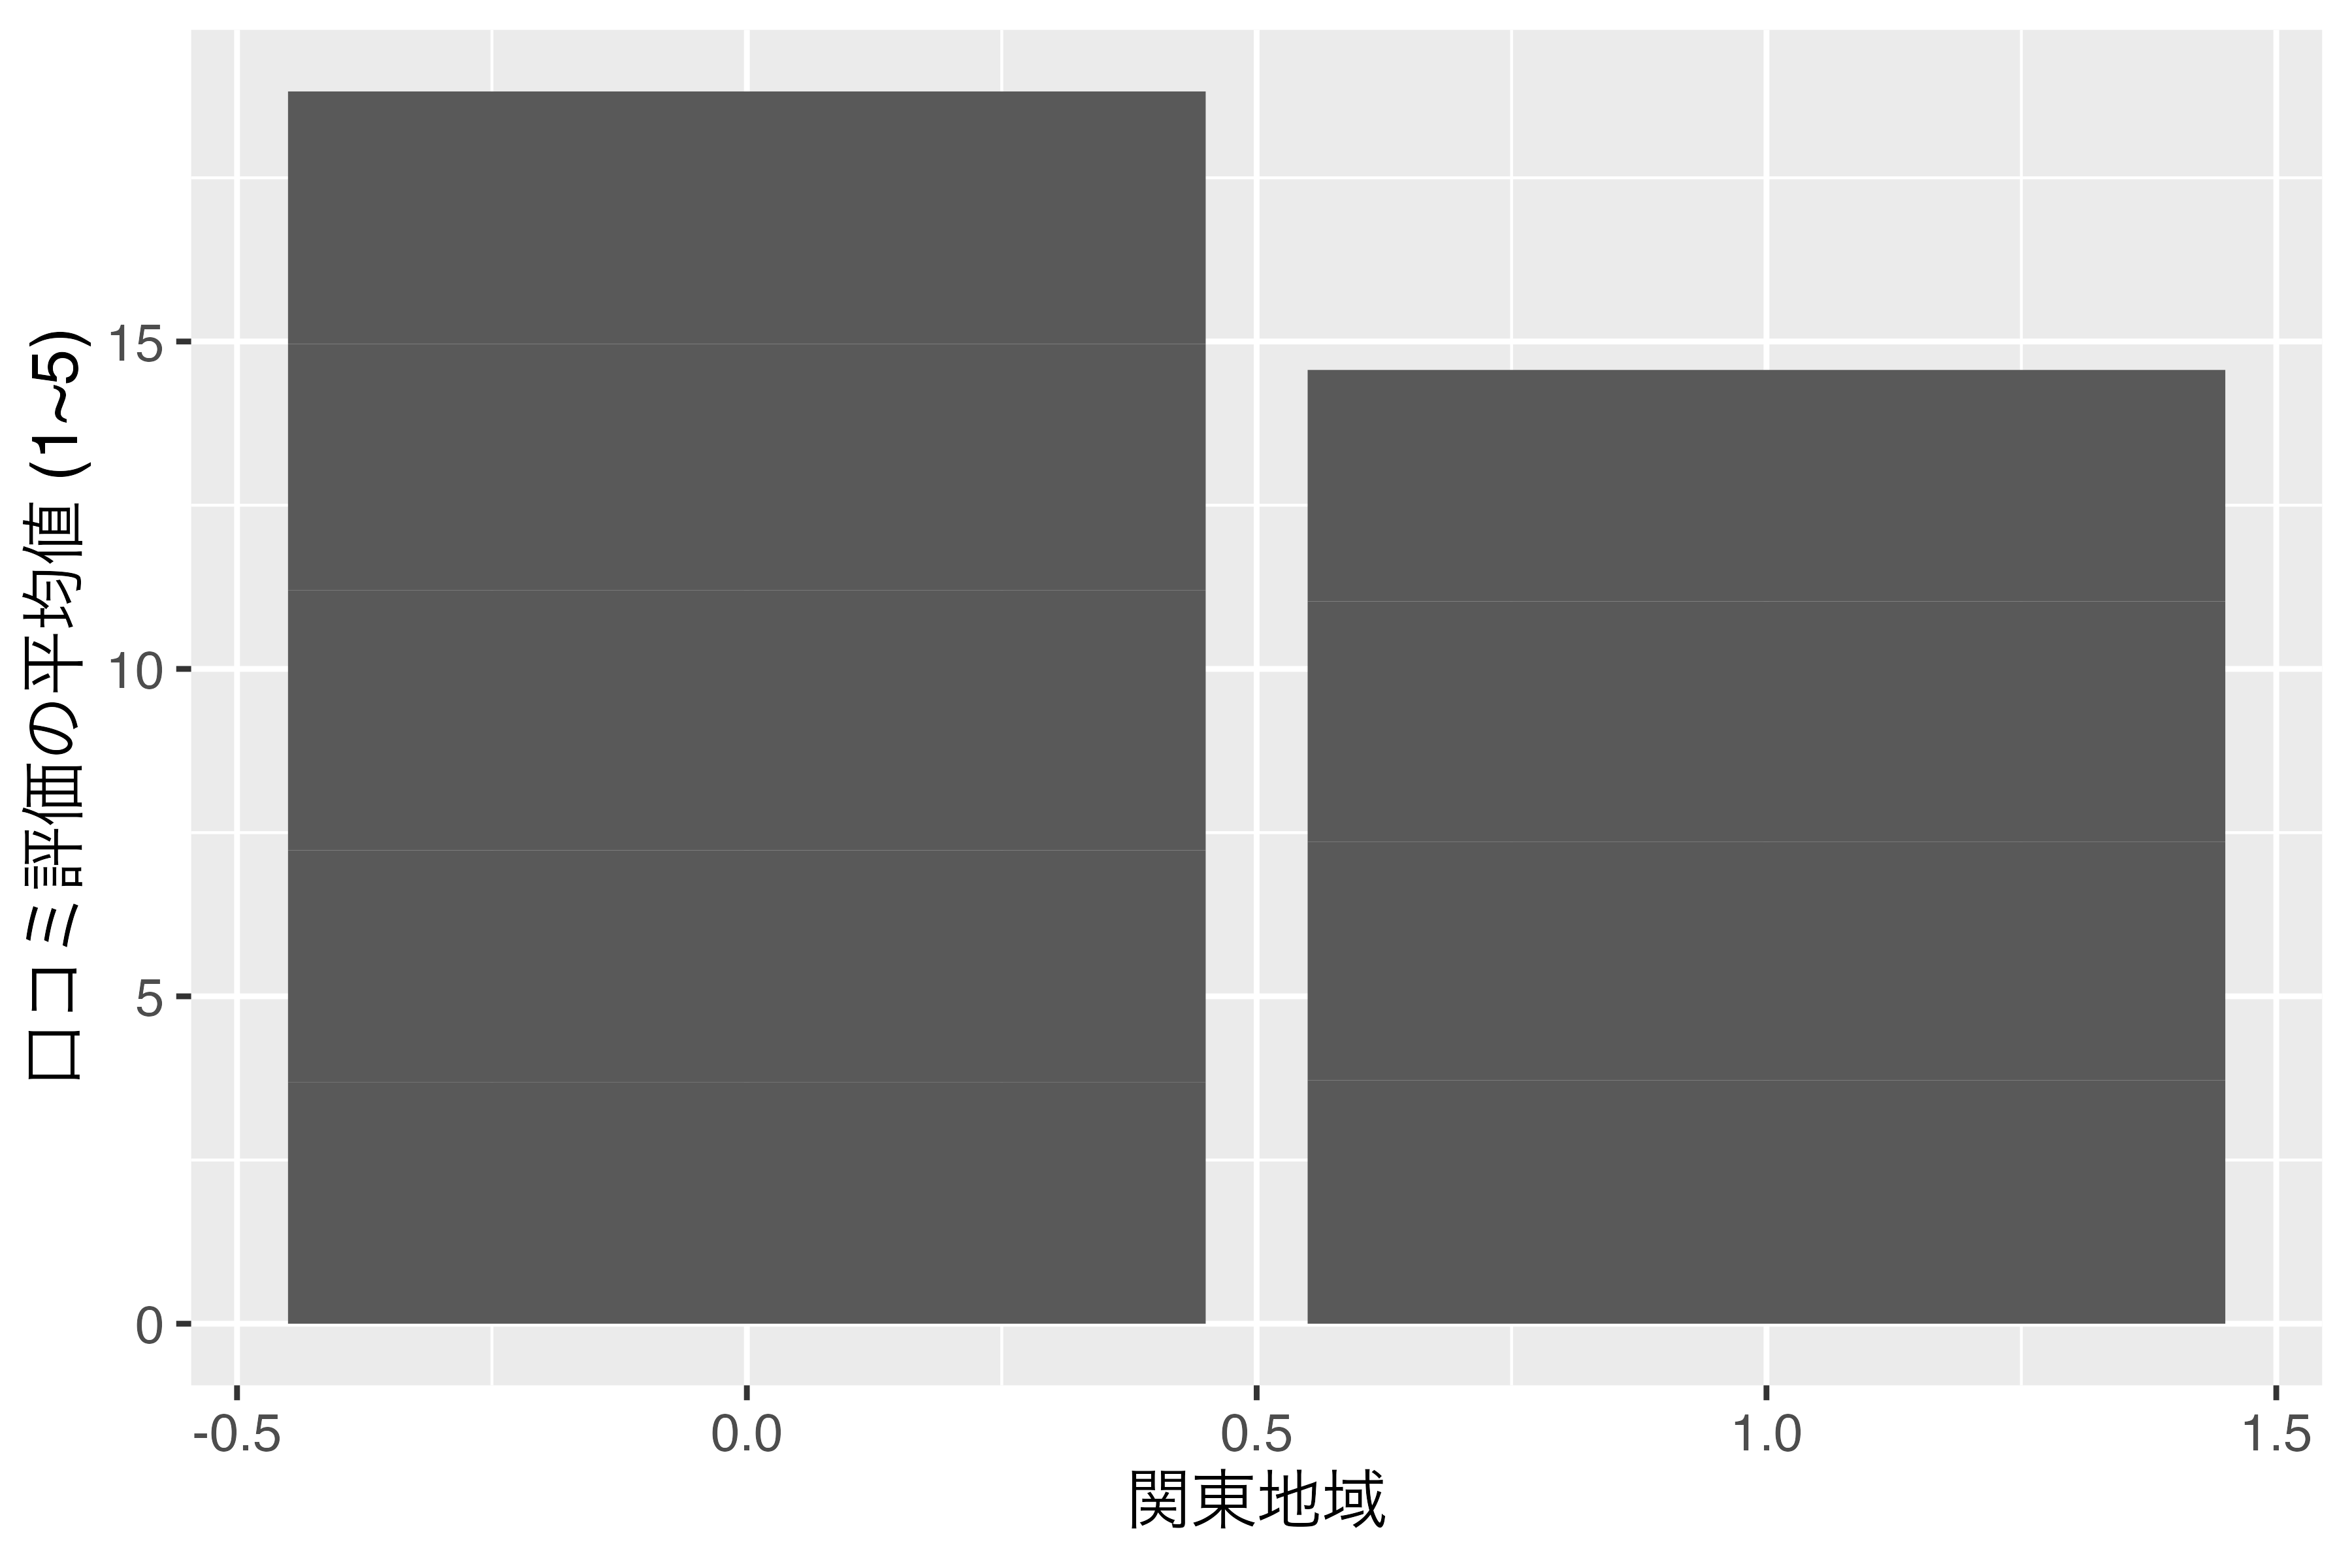
\includegraphics{./factor_files/figure-pdf/fig-factor5-1.png}

}

\caption{\label{fig-factor5}Kantoがnumeric型の場合}

\end{figure}

この場合、図の横軸は\texttt{Kanto}の値が小さい順でソートされます。ただし、このような図は非常に見にくいため、\texttt{1}に\texttt{"関東"}、\texttt{0}に\texttt{"関西"}とラベルを付けたfactor型に変換した方が望ましいです。numeric型をラベル付きのfactor型にするためには、\texttt{levels}引数には元の数値を、\texttt{labels}引数にはそれぞれの数値に対応したラベルを指定します。また、関東の方を先に出したいので、\texttt{factor()}内の\texttt{levels}引数は\texttt{c(0,\ 1)}でなく、\texttt{c(1,\ 0)}にします。

\begin{Shaded}
\begin{Highlighting}[numbers=left,,]
\NormalTok{Score\_df\_f1 }\OtherTok{\textless{}{-}}\NormalTok{ Score\_df\_f1 }\SpecialCharTok{\%\textgreater{}\%}
  \FunctionTok{mutate}\NormalTok{(}\AttributeTok{Kanto =} \FunctionTok{factor}\NormalTok{(Kanto, }\AttributeTok{levels =} \FunctionTok{c}\NormalTok{(}\DecValTok{1}\NormalTok{, }\DecValTok{0}\NormalTok{), }\AttributeTok{labels =} \FunctionTok{c}\NormalTok{(}\StringTok{"関東"}\NormalTok{, }\StringTok{"その他"}\NormalTok{)))}

\NormalTok{Score\_df\_f1}
\end{Highlighting}
\end{Shaded}

\begin{verbatim}
# A tibble: 9 x 3
  Pref     Score Kanto 
  <fct>    <dbl> <fct> 
1 京都府    3.68 その他
2 兵庫県    3.54 その他
3 千葉県    3.72 関東  
4 和歌山県  3.97 その他
5 埼玉県    3.64 関東  
6 大阪府    3.77 その他
7 奈良県    3.85 その他
8 東京都    3.67 関東  
9 神奈川県  3.53 関東  
\end{verbatim}

\texttt{Kanto}変数がfactor型に変換されたことが分かります。

\begin{Shaded}
\begin{Highlighting}[numbers=left,,]
\NormalTok{Score\_df\_f1}\SpecialCharTok{$}\NormalTok{Kanto}
\end{Highlighting}
\end{Shaded}

\begin{verbatim}
[1] その他 その他 関東   その他 関東   その他 その他 関東   関東  
Levels: 関東 その他
\end{verbatim}

また、\texttt{"関東"}、\texttt{"その他"}の順になっていますね。これを図として出力した結果が
図~\ref{fig-factor6} です。

\begin{figure}

{\centering 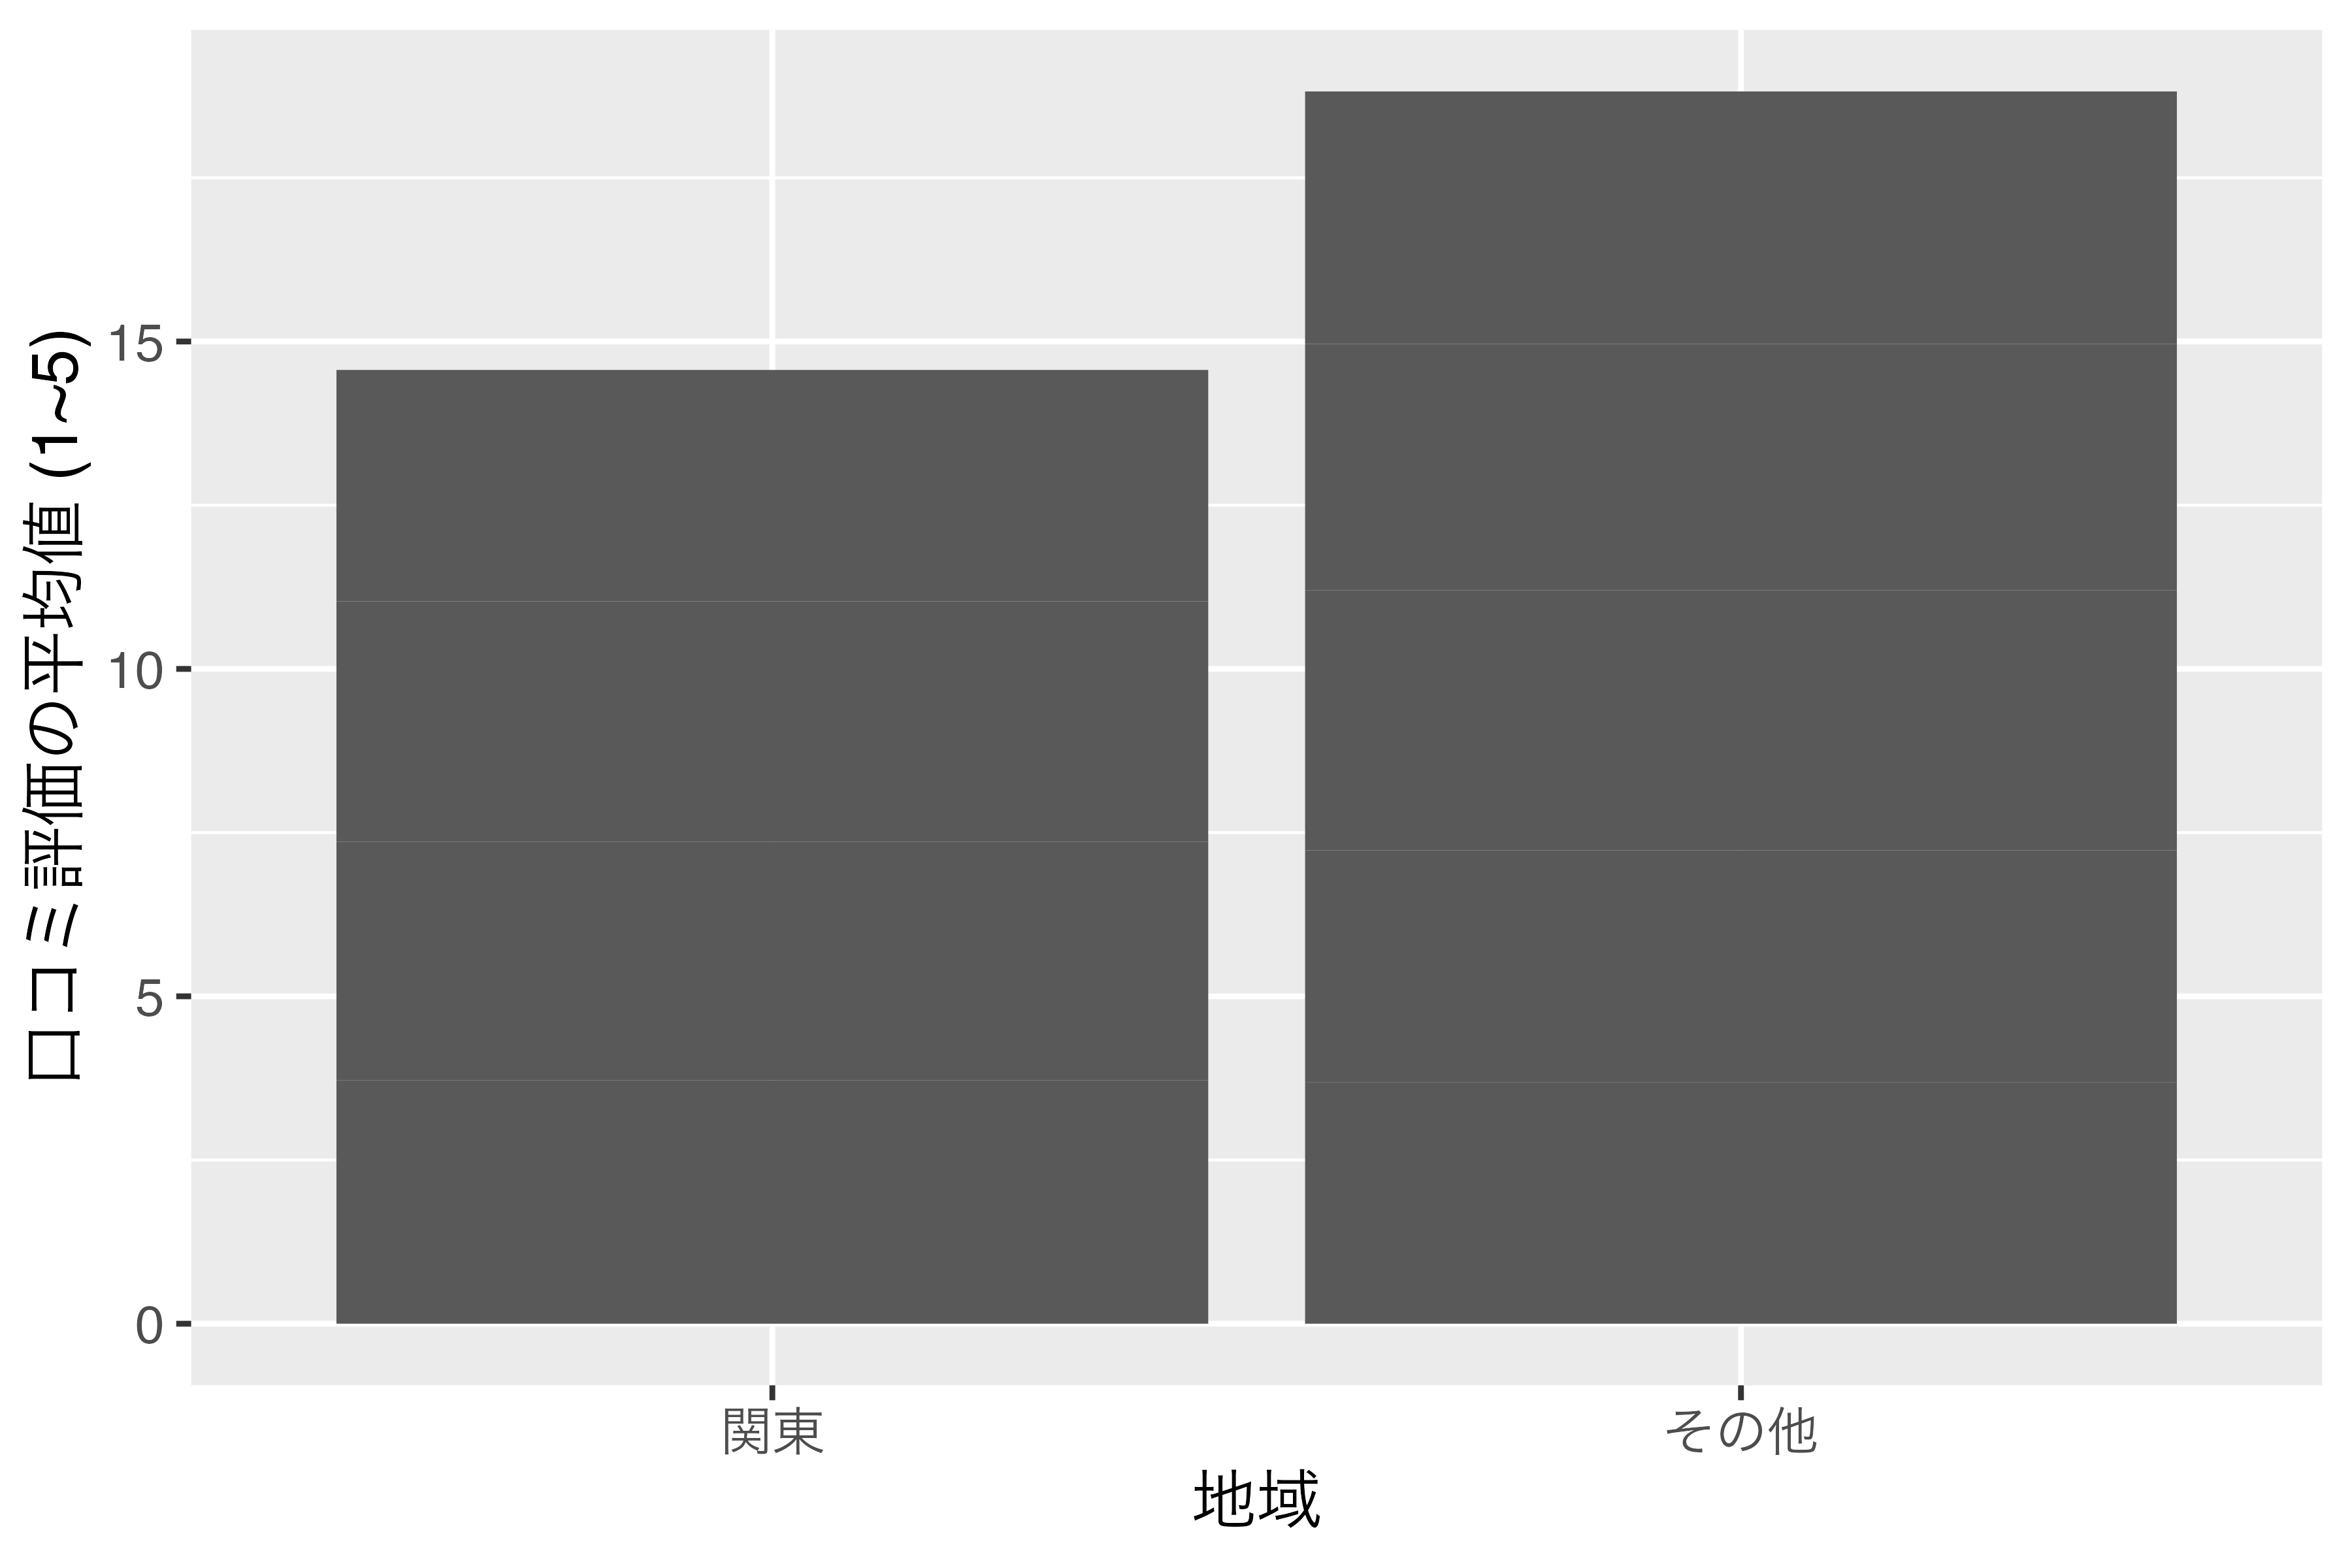
\includegraphics{./factor_files/figure-pdf/fig-factor6-1.png}

}

\caption{\label{fig-factor6}Kantoがfactor型の場合}

\end{figure}

このように数値型名目変数でも、factor化することによって、自由に横軸の順番を変えることができます。それでは、factor化に使える便利な関数をいくつか紹介します。

\hypertarget{forcatsux30d1ux30c3ux30b1ux30fcux30b8ux306bux3064ux3044ux3066}{%
\section{\texorpdfstring{\texttt{forcats}パッケージについて}{forcatsパッケージについて}}\label{forcatsux30d1ux30c3ux30b1ux30fcux30b8ux306bux3064ux3044ux3066}}

実はfactor型への変換や、順番に変更などは全てR内蔵の\texttt{factor()}関数で対応可能ですが、ここでは\texttt{forcats}パッケージが提供している\texttt{fct\_*()}関数を使用します。\texttt{forcats}パッケージは\texttt{tidyverse}を読み込む際、自動的に読み込まれるため、既に\texttt{tidyverse}を読み込んでいる場合、別途のコードは要りません。

\hypertarget{fct_relevel-ux6c34ux6e96ux306eux9806ux756aux3092ux5909ux66f4ux3059ux308b}{%
\subsection{\texorpdfstring{\texttt{fct\_relevel()}:
水準の順番を変更する}{fct\_relevel(): 水準の順番を変更する}}\label{fct_relevel-ux6c34ux6e96ux306eux9806ux756aux3092ux5909ux66f4ux3059ux308b}}

\texttt{Score\_df\_f1}の\texttt{f1}は\texttt{Score}が高い順になっています。これを50音順に変更する際、\texttt{fct\_relevel()}関数を使います。

\begin{Shaded}
\begin{Highlighting}[numbers=left,,]
\CommentTok{\# 新しい変数名と元となる変数名が一致すると上書きになる}
\NormalTok{データフレーム名 }\SpecialCharTok{\%\textgreater{}\%}
  \FunctionTok{mutate}\NormalTok{(新しい変数名 }\OtherTok{=} \FunctionTok{fct\_releve}\NormalTok{(元となる変数名, }
                                    \StringTok{"水準1"}\NormalTok{, }\StringTok{"水準2"}\NormalTok{, }\StringTok{"水準3"}\NormalTok{, ...))}
\end{Highlighting}
\end{Shaded}

ここでは、\texttt{Pref}変数を再調整した\texttt{Pref2}変数を作ってみましょう。

\begin{Shaded}
\begin{Highlighting}[numbers=left,,]
\NormalTok{Score\_df\_f1 }\OtherTok{\textless{}{-}}\NormalTok{ Score\_df\_f1 }\SpecialCharTok{\%\textgreater{}\%}
  \FunctionTok{mutate}\NormalTok{(}\AttributeTok{Pref2 =} \FunctionTok{fct\_relevel}\NormalTok{(Pref, }\StringTok{"大阪府"}\NormalTok{, }\StringTok{"神奈川県"}\NormalTok{, }\StringTok{"京都府"}\NormalTok{, }
                             \StringTok{"埼玉県"}\NormalTok{, }\StringTok{"千葉県"}\NormalTok{, }\StringTok{"東京都"}\NormalTok{, }
                             \StringTok{"奈良県"}\NormalTok{, }\StringTok{"兵庫県"}\NormalTok{, }\StringTok{"和歌山県"}\NormalTok{))}

\NormalTok{Score\_df\_f1}
\end{Highlighting}
\end{Shaded}

\begin{verbatim}
# A tibble: 9 x 4
  Pref     Score Kanto  Pref2   
  <fct>    <dbl> <fct>  <fct>   
1 京都府    3.68 その他 京都府  
2 兵庫県    3.54 その他 兵庫県  
3 千葉県    3.72 関東   千葉県  
4 和歌山県  3.97 その他 和歌山県
5 埼玉県    3.64 関東   埼玉県  
6 大阪府    3.77 その他 大阪府  
7 奈良県    3.85 その他 奈良県  
8 東京都    3.67 関東   東京都  
9 神奈川県  3.53 関東   神奈川県
\end{verbatim}

一見、\texttt{Pref}と\texttt{Pref2}変数は同じように見えますが、水準はどうなっているでしょうか。

\begin{Shaded}
\begin{Highlighting}[numbers=left,,]
\FunctionTok{levels}\NormalTok{(Score\_df\_f1}\SpecialCharTok{$}\NormalTok{Pref)  }\CommentTok{\# Prefの水準}
\end{Highlighting}
\end{Shaded}

\begin{verbatim}
[1] "和歌山県" "奈良県"   "大阪府"   "千葉県"   "京都府"   "東京都"   "埼玉県"  
[8] "兵庫県"   "神奈川県"
\end{verbatim}

\begin{Shaded}
\begin{Highlighting}[numbers=left,,]
\FunctionTok{levels}\NormalTok{(Score\_df\_f1}\SpecialCharTok{$}\NormalTok{Pref2) }\CommentTok{\# Pref2の水準}
\end{Highlighting}
\end{Shaded}

\begin{verbatim}
[1] "大阪府"   "神奈川県" "京都府"   "埼玉県"   "千葉県"   "東京都"   "奈良県"  
[8] "兵庫県"   "和歌山県"
\end{verbatim}

問題なく50音順になっていることが分かります。他にも\texttt{fct\_relevel()}には全ての水準名を指定する必要がありません。一部の水準名も可能です。たとえば、「関東が関西の先に来るなんでけしからん!」と思う読者もいるでしょう。この場合、関西の府県名を入れると、指定した水準が最初に位置するようになります。

\begin{Shaded}
\begin{Highlighting}[numbers=left,,]
\NormalTok{Score\_df\_f1 }\OtherTok{\textless{}{-}}\NormalTok{ Score\_df\_f1 }\SpecialCharTok{\%\textgreater{}\%}
  \FunctionTok{mutate}\NormalTok{(}\AttributeTok{Pref3 =} \FunctionTok{fct\_relevel}\NormalTok{(Pref, }\StringTok{"京都府"}\NormalTok{, }\StringTok{"大阪府"}\NormalTok{,}
                             \StringTok{"兵庫県"}\NormalTok{, }\StringTok{"奈良県"}\NormalTok{, }\StringTok{"和歌山県"}\NormalTok{))}

\FunctionTok{levels}\NormalTok{(Score\_df\_f1}\SpecialCharTok{$}\NormalTok{Pref3) }\CommentTok{\# Pref3の水準}
\end{Highlighting}
\end{Shaded}

\begin{verbatim}
[1] "京都府"   "大阪府"   "兵庫県"   "奈良県"   "和歌山県" "千葉県"   "東京都"  
[8] "埼玉県"   "神奈川県"
\end{verbatim}

一部の水準名のみを指定するとその水準が最初に移動されますが、\texttt{after}引数を指定すると、位置を調整することも可能です。\texttt{after\ =\ 2}の場合、元となる変数の1、3番目の水準は維持され、3番目以降に指定した水準、それに続いて指定されていない水準の順番になります。\texttt{Pref}は和歌山、奈良、大阪の順ですが、ここで京都と東京を、奈良と大阪の間に移動するなら、

\begin{Shaded}
\begin{Highlighting}[numbers=left,,]
\NormalTok{Score\_df\_f1 }\OtherTok{\textless{}{-}}\NormalTok{ Score\_df\_f1 }\SpecialCharTok{\%\textgreater{}\%}
  \FunctionTok{mutate}\NormalTok{(}\AttributeTok{Pref4 =} \FunctionTok{fct\_relevel}\NormalTok{(Pref, }\StringTok{"京都府"}\NormalTok{, }\StringTok{"東京都"}\NormalTok{, }\AttributeTok{after =} \DecValTok{2}\NormalTok{))}

\FunctionTok{levels}\NormalTok{(Score\_df\_f1}\SpecialCharTok{$}\NormalTok{Pref4) }\CommentTok{\# Pref4の水準}
\end{Highlighting}
\end{Shaded}

\begin{verbatim}
[1] "和歌山県" "奈良県"   "京都府"   "東京都"   "大阪府"   "千葉県"   "埼玉県"  
[8] "兵庫県"   "神奈川県"
\end{verbatim}

のように書きます。\texttt{after}を指定しない場合のデフォルト値は0であるため、最初に移動します。

\hypertarget{fct_recode-ux6c34ux6e96ux306eux30e9ux30d9ux30ebux3092ux5909ux66f4ux3059ux308b}{%
\subsection{\texorpdfstring{\texttt{fct\_recode()}:
水準のラベルを変更する}{fct\_recode(): 水準のラベルを変更する}}\label{fct_recode-ux6c34ux6e96ux306eux30e9ux30d9ux30ebux3092ux5909ux66f4ux3059ux308b}}

\texttt{fct\_recode()}は水準のラベルを変更する時に使う関数で、以下のように使います。

\begin{Shaded}
\begin{Highlighting}[numbers=left,,]
\CommentTok{\# 新しい変数名と元となる変数名が一致すると上書きになる}
\NormalTok{データフレーム名 }\SpecialCharTok{\%\textgreater{}\%}
  \FunctionTok{mutate}\NormalTok{(新しい変数名 }\OtherTok{=} \FunctionTok{fct\_recode}\NormalTok{(元となる変数名, }
\NormalTok{                                   新しいラベル1 }\OtherTok{=} \StringTok{"既存のラベル1"}\NormalTok{,}
\NormalTok{                                   新しいラベル2 }\OtherTok{=} \StringTok{"既存のラベル2"}\NormalTok{,}
\NormalTok{                                   新しいラベル3 }\OtherTok{=} \StringTok{"既存のラベル3"}\NormalTok{,}
\NormalTok{                                   ...))}
\end{Highlighting}
\end{Shaded}

注意点としては新しいラベルは\texttt{"}で囲まず、既存のラベルは\texttt{"}で囲む点です。それでは、\texttt{Pref}のラベルをローマ字に変更してみましょう。

\begin{Shaded}
\begin{Highlighting}[numbers=left,,]
\NormalTok{Score\_df\_f1 }\OtherTok{\textless{}{-}}\NormalTok{ Score\_df\_f1 }\SpecialCharTok{\%\textgreater{}\%}
  \FunctionTok{mutate}\NormalTok{(}\AttributeTok{Pref5 =} \FunctionTok{fct\_recode}\NormalTok{(Pref,}
                            \AttributeTok{Saitama  =} \StringTok{"埼玉県"}\NormalTok{,}
                            \AttributeTok{Wakayama =} \StringTok{"和歌山県"}\NormalTok{,}
                            \AttributeTok{Kyoto    =} \StringTok{"京都府"}\NormalTok{,}
                            \AttributeTok{Osaka    =} \StringTok{"大阪府"}\NormalTok{,}
                            \AttributeTok{Tokyo    =} \StringTok{"東京都"}\NormalTok{,}
                            \AttributeTok{Nara     =} \StringTok{"奈良県"}\NormalTok{,}
                            \AttributeTok{Kanagawa =} \StringTok{"神奈川県"}\NormalTok{,}
                            \AttributeTok{Hyogo    =} \StringTok{"兵庫県"}\NormalTok{,}
                            \AttributeTok{Chiba    =} \StringTok{"千葉県"}\NormalTok{))}

\NormalTok{Score\_df\_f1}
\end{Highlighting}
\end{Shaded}

\begin{verbatim}
# A tibble: 9 x 7
  Pref     Score Kanto  Pref2    Pref3    Pref4    Pref5   
  <fct>    <dbl> <fct>  <fct>    <fct>    <fct>    <fct>   
1 京都府    3.68 その他 京都府   京都府   京都府   Kyoto   
2 兵庫県    3.54 その他 兵庫県   兵庫県   兵庫県   Hyogo   
3 千葉県    3.72 関東   千葉県   千葉県   千葉県   Chiba   
4 和歌山県  3.97 その他 和歌山県 和歌山県 和歌山県 Wakayama
5 埼玉県    3.64 関東   埼玉県   埼玉県   埼玉県   Saitama 
6 大阪府    3.77 その他 大阪府   大阪府   大阪府   Osaka   
7 奈良県    3.85 その他 奈良県   奈良県   奈良県   Nara    
8 東京都    3.67 関東   東京都   東京都   東京都   Tokyo   
9 神奈川県  3.53 関東   神奈川県 神奈川県 神奈川県 Kanagawa
\end{verbatim}

\texttt{fct\_recode()}の中に指定する水準の順番は無視されます。つまり、水準の順番はそのまま維持されるため、好きな順番で結構です。また、全ての水準を指定せず、一部のみ変更することも可能です。それでは\texttt{Pref5}の順番が\texttt{Pref}の順番と同じかを確認してみましょう。

\begin{Shaded}
\begin{Highlighting}[numbers=left,,]
\FunctionTok{levels}\NormalTok{(Score\_df\_f1}\SpecialCharTok{$}\NormalTok{Pref)  }\CommentTok{\# Prefの水準}
\end{Highlighting}
\end{Shaded}

\begin{verbatim}
[1] "和歌山県" "奈良県"   "大阪府"   "千葉県"   "京都府"   "東京都"   "埼玉県"  
[8] "兵庫県"   "神奈川県"
\end{verbatim}

\begin{Shaded}
\begin{Highlighting}[numbers=left,,]
\FunctionTok{levels}\NormalTok{(Score\_df\_f1}\SpecialCharTok{$}\NormalTok{Pref5) }\CommentTok{\# Pref5の水準}
\end{Highlighting}
\end{Shaded}

\begin{verbatim}
[1] "Wakayama" "Nara"     "Osaka"    "Chiba"    "Kyoto"    "Tokyo"    "Saitama" 
[8] "Hyogo"    "Kanagawa"
\end{verbatim}

\hypertarget{fct_rev-ux6c34ux6e96ux306eux9806ux756aux3092ux53cdux8ee2ux3055ux305bux308b}{%
\subsection{\texorpdfstring{\texttt{fct\_rev()}:
水準の順番を反転させる}{fct\_rev(): 水準の順番を反転させる}}\label{fct_rev-ux6c34ux6e96ux306eux9806ux756aux3092ux53cdux8ee2ux3055ux305bux308b}}

水準の順番を反転することは非常によくあります。たとえば、グラフの読みやすさのために、左右または上下を反転するケースがあります。既に何回も強調しましたように、名目変数は基本的にfactor型にすべきであり、ここで\texttt{fct\_rev()}関数が非常に便利です。たとえば、\texttt{Pref2}の水準は50音順でありますが、これを反転し、\texttt{Pref6}という名の列として追加してみましょう。

\begin{Shaded}
\begin{Highlighting}[numbers=left,,]
\NormalTok{Score\_df\_f1 }\OtherTok{\textless{}{-}}\NormalTok{ Score\_df\_f1 }\SpecialCharTok{\%\textgreater{}\%}
  \FunctionTok{mutate}\NormalTok{(}\AttributeTok{Pref6 =} \FunctionTok{fct\_rev}\NormalTok{(Pref2))}

\FunctionTok{levels}\NormalTok{(Score\_df\_f1}\SpecialCharTok{$}\NormalTok{Pref6)}
\end{Highlighting}
\end{Shaded}

\begin{verbatim}
[1] "和歌山県" "兵庫県"   "奈良県"   "東京都"   "千葉県"   "埼玉県"   "京都府"  
[8] "神奈川県" "大阪府"  
\end{verbatim}

関数一つで水準の順番が反転されました。

\hypertarget{fct_infreq-ux983bux5ea6ux9806ux306bux9806ux756aux3092ux5909ux66f4ux3059ux308b}{%
\subsection{\texorpdfstring{\texttt{fct\_infreq()}:
頻度順に順番を変更する}{fct\_infreq(): 頻度順に順番を変更する}}\label{fct_infreq-ux983bux5ea6ux9806ux306bux9806ux756aux3092ux5909ux66f4ux3059ux308b}}

続いて、水準の順番を頻度順に合わせる\texttt{fct\_infreq()}関数です。たとえば、\texttt{Score}が欠損でないケースのみで構成された\texttt{df2}を考えてみましょう。

\begin{Shaded}
\begin{Highlighting}[numbers=left,,]
\NormalTok{df2 }\OtherTok{\textless{}{-}}\NormalTok{ df }\SpecialCharTok{\%\textgreater{}\%}
  \FunctionTok{filter}\NormalTok{(}\SpecialCharTok{!}\FunctionTok{is.na}\NormalTok{(Score))}
\end{Highlighting}
\end{Shaded}

そして、都府県ごとのケース数を計算します。

\begin{Shaded}
\begin{Highlighting}[numbers=left,,]
\FunctionTok{table}\NormalTok{(df2}\SpecialCharTok{$}\NormalTok{Pref)}
\end{Highlighting}
\end{Shaded}

\begin{verbatim}
  京都府   兵庫県   千葉県 和歌山県   埼玉県   大阪府   奈良県   東京都 
      79       85      108       24      118      175       28      298 
神奈川県 
     219 
\end{verbatim}

ここで\texttt{Pref}をfactor化しますが、水準の順番を店舗数が多い方を先にするにはどうすれば良いでしょうか。\texttt{fct\_infreq()}関数は指定された変数の各値の個数を計算し、多い順にfactorの水準を調整します。

\begin{Shaded}
\begin{Highlighting}[numbers=left,,]
\NormalTok{df2 }\OtherTok{\textless{}{-}}\NormalTok{ df2 }\SpecialCharTok{\%\textgreater{}\%}
  \CommentTok{\# 多く出現した値順でfactor化する}
  \FunctionTok{mutate}\NormalTok{(}\AttributeTok{Pref =} \FunctionTok{fct\_infreq}\NormalTok{(Pref))}

\FunctionTok{levels}\NormalTok{(df2}\SpecialCharTok{$}\NormalTok{Pref) }\CommentTok{\# df2のPref変数の水準を出力}
\end{Highlighting}
\end{Shaded}

\begin{verbatim}
[1] "東京都"   "神奈川県" "大阪府"   "埼玉県"   "千葉県"   "兵庫県"   "京都府"  
[8] "奈良県"   "和歌山県"
\end{verbatim}

\texttt{"東京都"}、\texttt{"神奈川県"}、\texttt{"大阪府"}、\ldots の順で水準の順番が調整され、これは\texttt{table(df\$Pref2)}の順位とも一致します。

\hypertarget{fct_inorder-ux30c7ux30fcux30bfux5185ux306eux51faux73feux9806ux756aux306bux9806ux756aux3092ux5909ux66f4ux3059ux308b}{%
\subsection{\texorpdfstring{\texttt{fct\_inorder()}:
データ内の出現順番に順番を変更する}{fct\_inorder(): データ内の出現順番に順番を変更する}}\label{fct_inorder-ux30c7ux30fcux30bfux5185ux306eux51faux73feux9806ux756aux306bux9806ux756aux3092ux5909ux66f4ux3059ux308b}}

続いて、\texttt{fct\_inorder()}ですが、これは意外と頻繁に使われる関数です。たとえば、自分でデータフレームなどを作成し、ケースの順番も綺麗に整えたとします。しかし、既に指摘した通り、データフレーム
(または、tibble)での順番とグラフにおける順番は一致するとは限りません。データフレームに格納された順番でfactorの水準が設定できれば非常に便利でしょう。そこで使うのが\texttt{fct\_inorder()}です。

たとえば、\texttt{df}の\texttt{Pref}は\texttt{"東京都"}が1000個並び、続いて\texttt{"神奈川県"}が1000個、\texttt{"千葉県"}が1000個、\ldots の順番で格納されています。この順番をそのままfactorの順番にするには以下のように書きます。

\begin{Shaded}
\begin{Highlighting}[numbers=left,,]
\NormalTok{df3 }\OtherTok{\textless{}{-}}\NormalTok{ df }\SpecialCharTok{\%\textgreater{}\%}
  \CommentTok{\# Pref変数をfactor化し、水準は出現順とする}
  \CommentTok{\# 変換後の結果はPrefに上書きする}
  \FunctionTok{mutate}\NormalTok{(}\AttributeTok{Pref =} \FunctionTok{fct\_inorder}\NormalTok{(Pref))}

\FunctionTok{levels}\NormalTok{(df3}\SpecialCharTok{$}\NormalTok{Pref)}
\end{Highlighting}
\end{Shaded}

\begin{verbatim}
[1] "東京都"   "神奈川県" "千葉県"   "埼玉県"   "大阪府"   "京都府"   "兵庫県"  
[8] "奈良県"   "和歌山県"
\end{verbatim}

\hypertarget{fct_shift-ux6c34ux6e96ux306eux9806ux756aux3092ux305aux3089ux3059}{%
\subsection{\texorpdfstring{\texttt{fct\_shift()}:
水準の順番をずらす}{fct\_shift(): 水準の順番をずらす}}\label{fct_shift-ux6c34ux6e96ux306eux9806ux756aux3092ux305aux3089ux3059}}

続いて、水準の順番をずらす\texttt{fct\_shift()}関数を紹介します。たとえば、「1:そう思う」〜「5:そう思わない」、「9:答えたくない」の6水準で構成された変数があるとします。

\begin{Shaded}
\begin{Highlighting}[numbers=left,,]
\NormalTok{df4 }\OtherTok{\textless{}{-}} \FunctionTok{tibble}\NormalTok{(}
  \AttributeTok{ID =} \DecValTok{1}\SpecialCharTok{:}\DecValTok{10}\NormalTok{,}
  \AttributeTok{Q1 =} \FunctionTok{c}\NormalTok{(}\DecValTok{1}\NormalTok{, }\DecValTok{5}\NormalTok{, }\DecValTok{3}\NormalTok{, }\DecValTok{2}\NormalTok{, }\DecValTok{9}\NormalTok{, }\DecValTok{2}\NormalTok{, }\DecValTok{4}\NormalTok{, }\DecValTok{9}\NormalTok{, }\DecValTok{5}\NormalTok{, }\DecValTok{1}\NormalTok{)}
\NormalTok{) }

\NormalTok{df4 }\OtherTok{\textless{}{-}}\NormalTok{ df4 }\SpecialCharTok{\%\textgreater{}\%}
  \FunctionTok{mutate}\NormalTok{(}\AttributeTok{Q1 =} \FunctionTok{factor}\NormalTok{(Q1, }\AttributeTok{levels =} \FunctionTok{c}\NormalTok{(}\DecValTok{1}\SpecialCharTok{:}\DecValTok{5}\NormalTok{, }\DecValTok{9}\NormalTok{),}
                     \AttributeTok{labels =} \FunctionTok{c}\NormalTok{(}\StringTok{"そう思う"}\NormalTok{, }
                                \StringTok{"どちらかと言えばそう思う"}\NormalTok{,}
                                \StringTok{"どちらとも言えない"}\NormalTok{,}
                                \StringTok{"どちらかと言えばそう思わない"}\NormalTok{,}
                                \StringTok{"そう思わない"}\NormalTok{,}
                                \StringTok{"答えたくない"}\NormalTok{)))}

\NormalTok{df4}
\end{Highlighting}
\end{Shaded}

\begin{verbatim}
# A tibble: 10 x 2
      ID Q1                          
   <int> <fct>                       
 1     1 そう思う                    
 2     2 そう思わない                
 3     3 どちらとも言えない          
 4     4 どちらかと言えばそう思う    
 5     5 答えたくない                
 6     6 どちらかと言えばそう思う    
 7     7 どちらかと言えばそう思わない
 8     8 答えたくない                
 9     9 そう思わない                
10    10 そう思う                    
\end{verbatim}

水準の順番も「そう思う」〜「答えたくない」順で綺麗に整っています。この水準を反転するには\texttt{fct\_rev()}関数が便利です。\texttt{Q1}の水準を反転した変数を\texttt{Q1\_R}という新しい列として追加し、水準を確認してみましょう。

\begin{Shaded}
\begin{Highlighting}[numbers=left,,]
\NormalTok{df4 }\OtherTok{\textless{}{-}}\NormalTok{ df4 }\SpecialCharTok{\%\textgreater{}\%}
  \FunctionTok{mutate}\NormalTok{(}\AttributeTok{Q1\_R =} \FunctionTok{fct\_rev}\NormalTok{(Q1))}

\NormalTok{df4}
\end{Highlighting}
\end{Shaded}

\begin{verbatim}
# A tibble: 10 x 3
      ID Q1                           Q1_R                        
   <int> <fct>                        <fct>                       
 1     1 そう思う                     そう思う                    
 2     2 そう思わない                 そう思わない                
 3     3 どちらとも言えない           どちらとも言えない          
 4     4 どちらかと言えばそう思う     どちらかと言えばそう思う    
 5     5 答えたくない                 答えたくない                
 6     6 どちらかと言えばそう思う     どちらかと言えばそう思う    
 7     7 どちらかと言えばそう思わない どちらかと言えばそう思わない
 8     8 答えたくない                 答えたくない                
 9     9 そう思わない                 そう思わない                
10    10 そう思う                     そう思う                    
\end{verbatim}

\begin{Shaded}
\begin{Highlighting}[numbers=left,,]
\FunctionTok{levels}\NormalTok{(df4}\SpecialCharTok{$}\NormalTok{Q1\_R)}
\end{Highlighting}
\end{Shaded}

\begin{verbatim}
[1] "答えたくない"                 "そう思わない"                
[3] "どちらかと言えばそう思わない" "どちらとも言えない"          
[5] "どちらかと言えばそう思う"     "そう思う"                    
\end{verbatim}

「答えたくない」が最初の順番に来ましてね。できれば、「そう思わない」〜「そう思う」、「答えたくない」の順番にしたいところです。ここで使うのが\texttt{fct\_shift()}ですが、書き方がややこしいので、噛み砕いて解説します。

\begin{Shaded}
\begin{Highlighting}[numbers=left,,]
\CommentTok{\# fct\_shift()の使い方}
\NormalTok{データ名 }\SpecialCharTok{\%\textgreater{}\%}
  \FunctionTok{mutate}\NormalTok{(新しい変数名 }\OtherTok{=} \FunctionTok{fct\_shift}\NormalTok{(元の変数名, }\AttributeTok{n =}\NormalTok{ 左方向へずらす個数))}
\end{Highlighting}
\end{Shaded}

問題は\texttt{n\ =}引数ですが、その挙動については 表~\ref{tbl-factor1}
を参照してください。

\hypertarget{tbl-factor1}{}
\begin{table}
\caption{\label{tbl-factor1}fct shift()の仕組み }

\centering
\begin{tabular}{l|c|c|c|c|c|c}
\hline
水準の順番 & 1番目 & 2番目 & 3番目 & 4番目 & 5番目 & 6番目\\
\hline
`n = -2` & `E` & `F` & `A` & `B` & `C` & `D`\\
\hline
`n = -1` & `F` & `A` & `B` & `C` & `D` & `E`\\
\hline
`n = 0` & `A` & `B` & `C` & `D` & `E` & `F`\\
\hline
`n = 1` & `B` & `C` & `D` & `E` & `F` & `A`\\
\hline
`n = 2` & `C` & `D` & `E` & `F` & `A` & `B`\\
\hline
\end{tabular}
\end{table}

具体的には水準は左方向へ\texttt{n}個移動します。元の水準が\texttt{A},
\texttt{B}, \texttt{C}, \ldots,
\texttt{F}の順で、\texttt{n\ =\ 1}の場合、\texttt{A}が\texttt{F}の後ろへ移動し、\texttt{B},
\texttt{C}, \texttt{D}, \texttt{E},
\texttt{F}が前の方へ1つずつ移動します。逆に右側へ1つ移動したい場合は\texttt{n\ =\ -1}のように書きます。今回は最初の水準を最後に移動させたいので、\texttt{n\ =\ 1}と指定します。

\begin{Shaded}
\begin{Highlighting}[numbers=left,,]
\NormalTok{df4 }\OtherTok{\textless{}{-}}\NormalTok{ df4 }\SpecialCharTok{\%\textgreater{}\%}
  \CommentTok{\# Q1\_Rの水準を左方向で1ずらす}
  \FunctionTok{mutate}\NormalTok{(}\AttributeTok{Q1\_R =} \FunctionTok{fct\_shift}\NormalTok{(Q1\_R, }\AttributeTok{n =} \DecValTok{1}\NormalTok{))}

\FunctionTok{levels}\NormalTok{(df4}\SpecialCharTok{$}\NormalTok{Q1\_R)}
\end{Highlighting}
\end{Shaded}

\begin{verbatim}
[1] "そう思わない"                 "どちらかと言えばそう思わない"
[3] "どちらとも言えない"           "どちらかと言えばそう思う"    
[5] "そう思う"                     "答えたくない"                
\end{verbatim}

これで水準の反転が完了しました。\texttt{fct\_shift()}はこのように世論調査データの処理に便利ですが、他にも曜日の処理に使えます。例えば、1週間の始まりを月曜にするか日曜にするかによって、\texttt{fct\_shift()}を使うケースがあります。

\hypertarget{fct_shuffle-ux6c34ux6e96ux306eux9806ux756aux3092ux30e9ux30f3ux30c0ux30e0ux5316ux3059ux308b}{%
\subsection{\texorpdfstring{\texttt{fct\_shuffle()}:
水準の順番をランダム化する}{fct\_shuffle(): 水準の順番をランダム化する}}\label{fct_shuffle-ux6c34ux6e96ux306eux9806ux756aux3092ux30e9ux30f3ux30c0ux30e0ux5316ux3059ux308b}}

あまり使わない機能ですが、水準の順番をランダム化することも可能です。使い方は非常に簡単で、\texttt{fct\_shuffle()}に元の変数名を入れるだけです。たとえば、\texttt{Score\_df}の\texttt{Pref}の順番をランダム化し、\texttt{Pref2}として追加します。同じことをもう2回繰り返し、それぞれ\texttt{Pref3}と\texttt{Pref4}という名前で追加してみましょう。

\begin{Shaded}
\begin{Highlighting}[numbers=left,,]
\NormalTok{Score\_df }\OtherTok{\textless{}{-}}\NormalTok{ Score\_df }\SpecialCharTok{\%\textgreater{}\%}
  \FunctionTok{mutate}\NormalTok{(}\AttributeTok{Pref2 =} \FunctionTok{fct\_shuffle}\NormalTok{(Pref),}
         \AttributeTok{Pref3 =} \FunctionTok{fct\_shuffle}\NormalTok{(Pref),}
         \AttributeTok{Pref4 =} \FunctionTok{fct\_shuffle}\NormalTok{(Pref))}

\NormalTok{Score\_df}
\end{Highlighting}
\end{Shaded}

\begin{verbatim}
# A tibble: 9 x 5
  Pref     Score Pref2    Pref3    Pref4   
  <chr>    <dbl> <fct>    <fct>    <fct>   
1 京都府    3.68 京都府   京都府   京都府  
2 兵庫県    3.54 兵庫県   兵庫県   兵庫県  
3 千葉県    3.72 千葉県   千葉県   千葉県  
4 和歌山県  3.97 和歌山県 和歌山県 和歌山県
5 埼玉県    3.64 埼玉県   埼玉県   埼玉県  
6 大阪府    3.77 大阪府   大阪府   大阪府  
7 奈良県    3.85 奈良県   奈良県   奈良県  
8 東京都    3.67 東京都   東京都   東京都  
9 神奈川県  3.53 神奈川県 神奈川県 神奈川県
\end{verbatim}

\begin{Shaded}
\begin{Highlighting}[numbers=left,,]
\FunctionTok{levels}\NormalTok{(Score\_df}\SpecialCharTok{$}\NormalTok{Pref2)}
\end{Highlighting}
\end{Shaded}

\begin{verbatim}
[1] "和歌山県" "奈良県"   "兵庫県"   "大阪府"   "京都府"   "千葉県"   "神奈川県"
[8] "埼玉県"   "東京都"  
\end{verbatim}

\begin{Shaded}
\begin{Highlighting}[numbers=left,,]
\FunctionTok{levels}\NormalTok{(Score\_df}\SpecialCharTok{$}\NormalTok{Pref3)}
\end{Highlighting}
\end{Shaded}

\begin{verbatim}
[1] "奈良県"   "埼玉県"   "兵庫県"   "大阪府"   "神奈川県" "和歌山県" "千葉県"  
[8] "東京都"   "京都府"  
\end{verbatim}

\begin{Shaded}
\begin{Highlighting}[numbers=left,,]
\FunctionTok{levels}\NormalTok{(Score\_df}\SpecialCharTok{$}\NormalTok{Pref4)}
\end{Highlighting}
\end{Shaded}

\begin{verbatim}
[1] "和歌山県" "京都府"   "奈良県"   "東京都"   "千葉県"   "神奈川県" "兵庫県"  
[8] "埼玉県"   "大阪府"  
\end{verbatim}

\texttt{Pref}から\texttt{Pref4}まで同じように見えますが、水準の順番が異なります
(\texttt{Pref}はcharacter型だから水準がありません)。

\hypertarget{fct_reorder-ux5225ux306e1ux5909ux6570ux306eux5024ux3092ux57faux6e96ux306bux6c34ux6e96ux306eux9806ux756aux3092ux5909ux66f4ux3059ux308b}{%
\subsection{\texorpdfstring{\texttt{fct\_reorder()}:
別の1変数の値を基準に水準の順番を変更する}{fct\_reorder(): 別の1変数の値を基準に水準の順番を変更する}}\label{fct_reorder-ux5225ux306e1ux5909ux6570ux306eux5024ux3092ux57faux6e96ux306bux6c34ux6e96ux306eux9806ux756aux3092ux5909ux66f4ux3059ux308b}}

\texttt{fct\_infreq()}は出現頻度順に並び替える関数でしたが、それと似たような関数として\texttt{fct\_reorder()}があります。ただし、これは出現頻度を基準にするのではなく、ある変数の平均値が低い順、中央値が高い順などでソートされます。まずは使い方から確認します。

\begin{Shaded}
\begin{Highlighting}[numbers=left,,]
\NormalTok{データ名 }\SpecialCharTok{\%\textgreater{}\%}
  \FunctionTok{mutate}\NormalTok{(新しい変数名 }\OtherTok{=} \FunctionTok{fct\_reorder}\NormalTok{(元の変数名, 基準となる変数, }
\NormalTok{                                   関数名, 関数の引数))}
\end{Highlighting}
\end{Shaded}

必要な引数が多いですね。解説よりも実際の例を見ながら説明します。今回も\texttt{Pref}をfactor変数にし、\texttt{Pref\_R}という列で格納しますが、平均予算が安い順でfactorの水準を決めたいと思います。

\begin{Shaded}
\begin{Highlighting}[numbers=left,,]
\NormalTok{df }\OtherTok{\textless{}{-}}\NormalTok{ df }\SpecialCharTok{\%\textgreater{}\%}
  \FunctionTok{mutate}\NormalTok{(}\AttributeTok{Pref\_R =} \FunctionTok{fct\_reorder}\NormalTok{(Pref, Budget, mean, }\AttributeTok{na.rm =} \ConstantTok{TRUE}\NormalTok{))}

\FunctionTok{levels}\NormalTok{(df}\SpecialCharTok{$}\NormalTok{Pref\_R)}
\end{Highlighting}
\end{Shaded}

\begin{verbatim}
[1] "千葉県"   "埼玉県"   "奈良県"   "兵庫県"   "大阪府"   "神奈川県" "和歌山県"
[8] "東京都"   "京都府"  
\end{verbatim}

\texttt{Pref\_R}の水準は千葉県、埼玉県、奈良県、\ldots の順ですが、本当にそうでしょうか。\texttt{group\_by()}と\texttt{summarise()}などを使って確認してみましょう。

\begin{Shaded}
\begin{Highlighting}[numbers=left,,]
\NormalTok{df }\SpecialCharTok{\%\textgreater{}\%} 
  \FunctionTok{group\_by}\NormalTok{(Pref) }\SpecialCharTok{\%\textgreater{}\%}
  \FunctionTok{summarise}\NormalTok{(}\AttributeTok{Budget  =} \FunctionTok{mean}\NormalTok{(Budget, }\AttributeTok{na.rm =} \ConstantTok{TRUE}\NormalTok{),}
            \AttributeTok{.groups =} \StringTok{"drop"}\NormalTok{) }\SpecialCharTok{\%\textgreater{}\%}
  \FunctionTok{arrange}\NormalTok{(Budget)}
\end{Highlighting}
\end{Shaded}

\begin{verbatim}
# A tibble: 9 x 2
  Pref     Budget
  <chr>     <dbl>
1 千葉県    1124.
2 埼玉県    1147.
3 奈良県    1169.
4 兵庫県    1197.
5 大阪府    1203.
6 神奈川県  1239.
7 和歌山県  1252 
8 東京都    1283.
9 京都府    1399.
\end{verbatim}

問題なくソートされましたね。注意点としては\texttt{fct\_reorder()}内に関数名を書く際、\texttt{()}は不要という点です。関数名の次の引数としてはその関数に別途必要な引数を指定します。引数が省略可能、あるいは不要な関数を使う場合は、省略しても構いませんし、数に制限はありません。

また、低い順ではなく、高い順にすることも可能です。次は\texttt{Score}の中央値が高い順に水準を設定した\texttt{Pref\_R2}を作ってみましょう。

\begin{Shaded}
\begin{Highlighting}[numbers=left,,]
\NormalTok{df }\OtherTok{\textless{}{-}}\NormalTok{ df }\SpecialCharTok{\%\textgreater{}\%}
  \FunctionTok{mutate}\NormalTok{(}\AttributeTok{Pref\_R2 =} \FunctionTok{fct\_reorder}\NormalTok{(Pref, Score, median, }\AttributeTok{na.rm =} \ConstantTok{TRUE}\NormalTok{, }\AttributeTok{.desc =} \ConstantTok{TRUE}\NormalTok{))}

\FunctionTok{levels}\NormalTok{(df}\SpecialCharTok{$}\NormalTok{Pref\_R2)}
\end{Highlighting}
\end{Shaded}

\begin{verbatim}
[1] "和歌山県" "奈良県"   "千葉県"   "大阪府"   "東京都"   "埼玉県"   "京都府"  
[8] "兵庫県"   "神奈川県"
\end{verbatim}

変わったのは\texttt{mean}の代わりに\texttt{median}を使ったこと、そして\texttt{.desc}引数が追加された点です。\texttt{fct\_reorder()}には\texttt{.desc\ =\ FALSE}がデフォルトとして指定されており、省略した場合は昇順でfactorの水準が決まります。ここで\texttt{.desc\ =\ TRUE}を指定すると、降順となります。実際、\texttt{Score}の中央値順になっているかを確認してみましょう。

\begin{Shaded}
\begin{Highlighting}[numbers=left,,]
\NormalTok{df }\SpecialCharTok{\%\textgreater{}\%} 
  \FunctionTok{group\_by}\NormalTok{(Pref) }\SpecialCharTok{\%\textgreater{}\%}
  \FunctionTok{summarise}\NormalTok{(}\AttributeTok{Score   =} \FunctionTok{median}\NormalTok{(Score, }\AttributeTok{na.rm =} \ConstantTok{TRUE}\NormalTok{),}
            \AttributeTok{.groups =} \StringTok{"drop"}\NormalTok{) }\SpecialCharTok{\%\textgreater{}\%}
  \FunctionTok{arrange}\NormalTok{(}\FunctionTok{desc}\NormalTok{(Score))}
\end{Highlighting}
\end{Shaded}

\begin{verbatim}
# A tibble: 9 x 2
  Pref     Score
  <chr>    <dbl>
1 和歌山県  4   
2 奈良県    3.88
3 千葉県    3.75
4 大阪府    3.75
5 東京都    3.64
6 埼玉県    3.61
7 京都府    3.5 
8 兵庫県    3.5 
9 神奈川県  3.5 
\end{verbatim}

\hypertarget{factor-forcat-reorder2}{%
\subsection{\texorpdfstring{\texttt{fct\_reorder2()}:
別の2変数の値を基準に水準の順番を変更する}{fct\_reorder2(): 別の2変数の値を基準に水準の順番を変更する}}\label{factor-forcat-reorder2}}

この関数は別の変数を基準に水準が調整される点では\texttt{fct\_reorder()}と類似しています。ただし、よく誤解されるのは「変数Aの値が同じなら変数Bを基準に\ldots」といったものではありません。たとえば、\texttt{fct\_reorder(x,\ y,\ mean)}の場合、\texttt{y}の平均値
(\texttt{mean()})の順で\texttt{x}の水準を調整するという意味です。この\texttt{mean()}関数に必要なデータはベクトル1つです。しかし、関数によっては2つの変数が必要な場合があります。

これは頻繁に直面する問題ではありませんが、この\texttt{fct\_reorder2()}関数が活躍するケースを紹介します。以下は6月27日から7月1日までの5日間、5地域におけるCOVID-19新規感染者数を表したデータです\footnote{データの出典は\href{https://news.google.com/covid19/map}{Google}です。}。入力が面倒な方は\href{Data/COVID19.csv}{ここ}からダウンロードして読み込んでください。

\begin{Shaded}
\begin{Highlighting}[numbers=left,,]
\CommentTok{\# 入力が面倒ならデータをダウンロードし、}
\CommentTok{\# Reorder2\_df \textless{}{-} read\_csv("Data/COVID19.csv")}
\NormalTok{Reorder2\_df }\OtherTok{\textless{}{-}} \FunctionTok{tibble}\NormalTok{(}
  \AttributeTok{Country =} \FunctionTok{rep}\NormalTok{(}\FunctionTok{c}\NormalTok{(}\StringTok{"日本"}\NormalTok{, }\StringTok{"韓国"}\NormalTok{, }\StringTok{"中国 (本土)"}\NormalTok{, }\StringTok{"台湾"}\NormalTok{, }\StringTok{"香港"}\NormalTok{),}
                \AttributeTok{each =} \DecValTok{5}\NormalTok{),}
  \AttributeTok{Date    =} \FunctionTok{rep}\NormalTok{(}\FunctionTok{c}\NormalTok{(}\StringTok{"2020/06/27"}\NormalTok{, }\StringTok{"2020/06/28"}\NormalTok{, }\StringTok{"2020/06/29"}\NormalTok{,}
                  \StringTok{"2020/06/30"}\NormalTok{, }\StringTok{"2020/07/01"}\NormalTok{), }\DecValTok{5}\NormalTok{),}
  \AttributeTok{NewPat  =} \FunctionTok{c}\NormalTok{(}\DecValTok{100}\NormalTok{, }\DecValTok{93}\NormalTok{, }\DecValTok{86}\NormalTok{, }\DecValTok{117}\NormalTok{, }\DecValTok{130}\NormalTok{, }
               \DecValTok{62}\NormalTok{, }\DecValTok{42}\NormalTok{, }\DecValTok{43}\NormalTok{,  }\DecValTok{50}\NormalTok{,  }\DecValTok{54}\NormalTok{,}
               \DecValTok{17}\NormalTok{, }\DecValTok{12}\NormalTok{, }\DecValTok{19}\NormalTok{,   }\DecValTok{3}\NormalTok{,   }\DecValTok{5}\NormalTok{,}
                \DecValTok{0}\NormalTok{,  }\DecValTok{0}\NormalTok{,  }\DecValTok{0}\NormalTok{,   }\DecValTok{0}\NormalTok{,   }\DecValTok{0}\NormalTok{,}
                \DecValTok{1}\NormalTok{,  }\DecValTok{2}\NormalTok{,  }\DecValTok{4}\NormalTok{,   }\DecValTok{2}\NormalTok{,  }\DecValTok{28}\NormalTok{)}
\NormalTok{)}

\NormalTok{Reorder2\_df }\OtherTok{\textless{}{-}}\NormalTok{ Reorder2\_df }\SpecialCharTok{\%\textgreater{}\%}
  \FunctionTok{mutate}\NormalTok{(}\AttributeTok{Date =} \FunctionTok{as.Date}\NormalTok{(Date))}

\NormalTok{Reorder2\_df}
\end{Highlighting}
\end{Shaded}

\begin{verbatim}
# A tibble: 25 x 3
   Country Date       NewPat
   <chr>   <date>      <dbl>
 1 日本    2020-06-27    100
 2 日本    2020-06-28     93
 3 日本    2020-06-29     86
 4 日本    2020-06-30    117
 5 日本    2020-07-01    130
 6 韓国    2020-06-27     62
 7 韓国    2020-06-28     42
 8 韓国    2020-06-29     43
 9 韓国    2020-06-30     50
10 韓国    2020-07-01     54
# ... with 15 more rows
\end{verbatim}

可視化のコードはとりあえず無視し、グラフを出力してみましょう。

\begin{Shaded}
\begin{Highlighting}[numbers=left,,]
\NormalTok{Reorder2\_df }\SpecialCharTok{\%\textgreater{}\%}
  \FunctionTok{ggplot}\NormalTok{() }\SpecialCharTok{+}
  \FunctionTok{geom\_line}\NormalTok{(}\FunctionTok{aes}\NormalTok{(}\AttributeTok{x =}\NormalTok{ Date, }\AttributeTok{y =}\NormalTok{ NewPat, }\AttributeTok{color =}\NormalTok{ Country),}
            \AttributeTok{size =} \DecValTok{1}\NormalTok{) }\SpecialCharTok{+}
  \FunctionTok{scale\_x\_date}\NormalTok{(}\AttributeTok{date\_labels =} \StringTok{"\%Y年\%m月\%d日"}\NormalTok{) }\SpecialCharTok{+}
  \FunctionTok{labs}\NormalTok{(}\AttributeTok{x =} \StringTok{"年月日"}\NormalTok{, }\AttributeTok{y =} \StringTok{"新規感染者数 (人)"}\NormalTok{, }\AttributeTok{color =} \StringTok{""}\NormalTok{) }\SpecialCharTok{+}
  \FunctionTok{theme\_gray}\NormalTok{(}\AttributeTok{base\_family =} \StringTok{"HiraKakuProN{-}W3"}\NormalTok{)}
\end{Highlighting}
\end{Shaded}

\begin{figure}[H]

{\centering 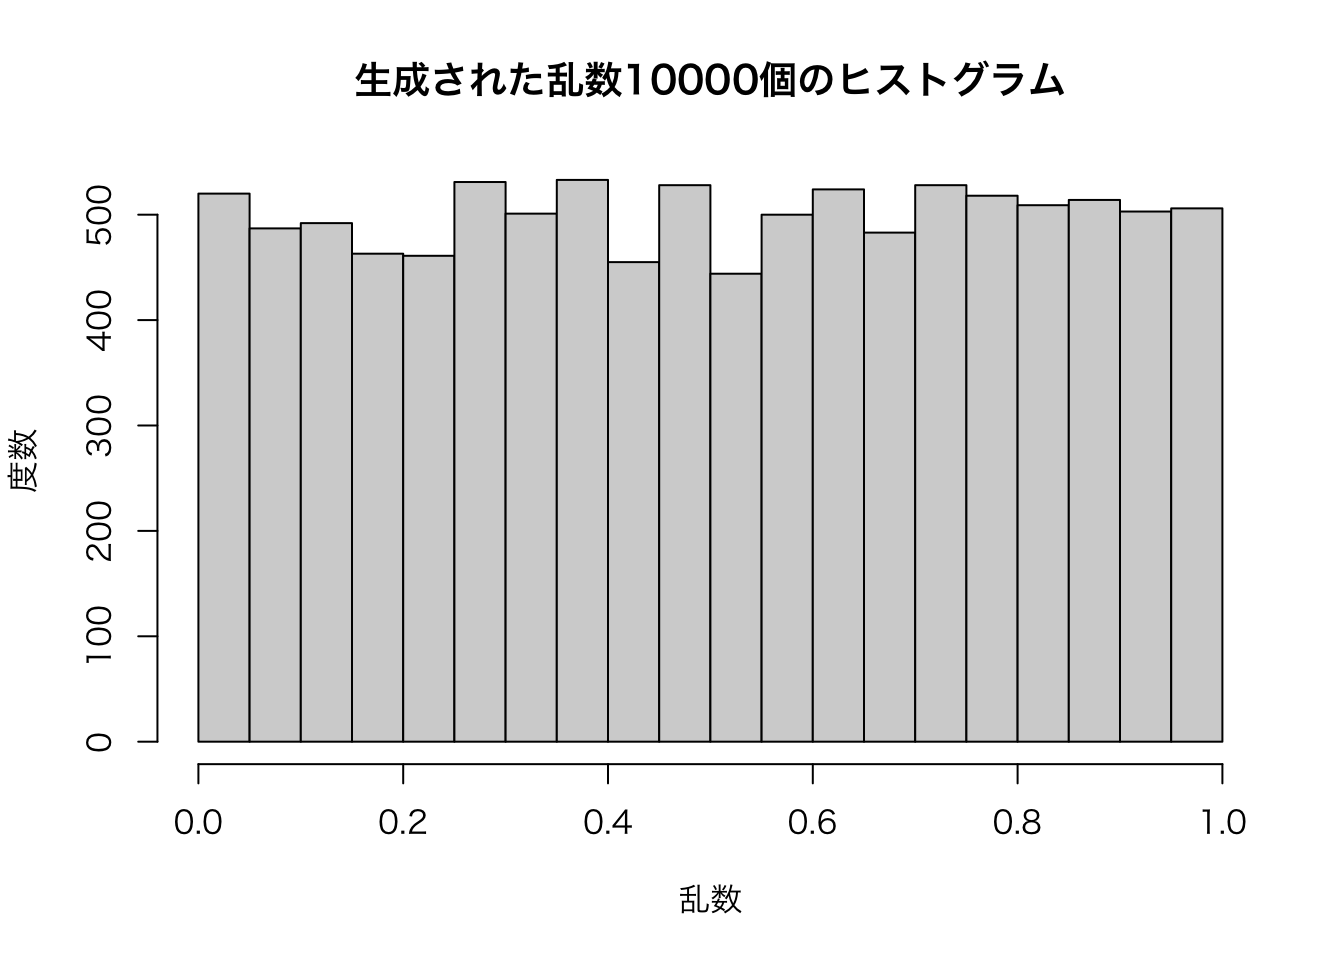
\includegraphics{./factor_files/figure-pdf/unnamed-chunk-75-1.png}

}

\end{figure}

このグラフに違和感はあまりありませんが、「読みやすさ」の麺では改善の余地があります。たとえば、7月1日の時点で、新規感染者数が多いのは日本、韓国、香港、中国
(本土)、台湾の順です。しかし、右側の凡例の順番はそうではありません。この順番が一致すれば、更に図は読みやすくなるでしょう。

\begin{Shaded}
\begin{Highlighting}[numbers=left,,]
\FunctionTok{factor}\NormalTok{(Reorder2\_df}\SpecialCharTok{$}\NormalTok{Country)}
\end{Highlighting}
\end{Shaded}

\begin{verbatim}
 [1] 日本        日本        日本        日本        日本        韓国       
 [7] 韓国        韓国        韓国        韓国        中国 (本土) 中国 (本土)
[13] 中国 (本土) 中国 (本土) 中国 (本土) 台湾        台湾        台湾       
[19] 台湾        台湾        香港        香港        香港        香港       
[25] 香港       
Levels: 中国 (本土) 台湾 日本 韓国 香港
\end{verbatim}

実際、何も指定せずに\texttt{Reorder2\_df}の\texttt{Country}をfactor化すると、韓国、香港、台湾、\ldots の順であり、これは上のグラフと一致します。これをグラフにおける7月1日の新規感染者数の順で並べるためには、\texttt{Date}を昇順にソートし、そして最後の要素
(\texttt{"2020/07/01"})内で新規感染者数
(\texttt{NewPat})を降順に並べ替えた場合の順番にする必要があります。実際、\texttt{Reorder2\_df}を\texttt{Date}で昇順、\texttt{NewPat}で降順にソートし、最後の5行を抽出した結果が以下のコードです。

\begin{Shaded}
\begin{Highlighting}[numbers=left,,]
\NormalTok{Reorder2\_df }\SpecialCharTok{\%\textgreater{}\%}
  \FunctionTok{arrange}\NormalTok{(Date, }\FunctionTok{desc}\NormalTok{(NewPat)) }\SpecialCharTok{\%\textgreater{}\%}
  \FunctionTok{slice\_tail}\NormalTok{(}\AttributeTok{n =} \DecValTok{5}\NormalTok{)}
\end{Highlighting}
\end{Shaded}

\begin{verbatim}
# A tibble: 5 x 3
  Country     Date       NewPat
  <chr>       <date>      <dbl>
1 日本        2020-07-01    130
2 韓国        2020-07-01     54
3 香港        2020-07-01     28
4 中国 (本土) 2020-07-01      5
5 台湾        2020-07-01      0
\end{verbatim}

このように、水準を調整する際に2つの変数
(\texttt{Date}と\texttt{NewPat})が使用されます。\texttt{fct\_reorder2()}は\texttt{fct\_reorder()}と買い方がほぼ同じですが、基準となる変数がもう一つ加わります。

\begin{Shaded}
\begin{Highlighting}[numbers=left,,]
\NormalTok{データ名 }\SpecialCharTok{\%\textgreater{}\%}
  \FunctionTok{mutate}\NormalTok{(新しい変数名 }\OtherTok{=} \FunctionTok{fct\_reorder2}\NormalTok{(元の変数名, }
\NormalTok{                                    基準となる変数1, 基準となる変数2,}
\NormalTok{                                    関数名, 関数の引数))}
\end{Highlighting}
\end{Shaded}

重要なのはここの関数のところですが、\texttt{fct\_reorder2()}はデフォルトで\texttt{last2()}という関数が指定されており、まさに私たちに必要な関数です。したがって、ここでは関数名も省略できますが、ここでは一応明記しておきます。

\begin{Shaded}
\begin{Highlighting}[numbers=left,,]
\NormalTok{Reorder2\_df }\OtherTok{\textless{}{-}}\NormalTok{ Reorder2\_df }\SpecialCharTok{\%\textgreater{}\%}
  \FunctionTok{mutate}\NormalTok{(}\AttributeTok{Country2 =} \FunctionTok{fct\_reorder2}\NormalTok{(Country, Date, NewPat, last2)) }
\end{Highlighting}
\end{Shaded}

それでは新しく出来た\texttt{Country2}の水準を確認してみましょう。

\begin{Shaded}
\begin{Highlighting}[numbers=left,,]
\FunctionTok{levels}\NormalTok{(Reorder2\_df}\SpecialCharTok{$}\NormalTok{Country2)}
\end{Highlighting}
\end{Shaded}

\begin{verbatim}
[1] "日本"        "韓国"        "香港"        "中国 (本土)" "台湾"       
\end{verbatim}

ちゃんと7月1日の新規感染者数基準で水準の順番が調整されましたので、これを使ってグラフをもう一回作ってみます。

\begin{Shaded}
\begin{Highlighting}[numbers=left,,]
\NormalTok{Reorder2\_df }\SpecialCharTok{\%\textgreater{}\%}
  \FunctionTok{ggplot}\NormalTok{() }\SpecialCharTok{+}
  \FunctionTok{geom\_line}\NormalTok{(}\FunctionTok{aes}\NormalTok{(}\AttributeTok{x =}\NormalTok{ Date, }\AttributeTok{y =}\NormalTok{ NewPat, }\AttributeTok{color =}\NormalTok{ Country2),}
            \AttributeTok{size =} \DecValTok{1}\NormalTok{) }\SpecialCharTok{+}
  \FunctionTok{scale\_x\_date}\NormalTok{(}\AttributeTok{date\_labels =} \StringTok{"\%Y年\%m月\%d日"}\NormalTok{) }\SpecialCharTok{+}
  \FunctionTok{labs}\NormalTok{(}\AttributeTok{x =} \StringTok{"年月日"}\NormalTok{, }\AttributeTok{y =} \StringTok{"新規感染者数 (人)"}\NormalTok{, }\AttributeTok{color =} \StringTok{""}\NormalTok{) }\SpecialCharTok{+}
  \FunctionTok{theme\_gray}\NormalTok{(}\AttributeTok{base\_family =} \StringTok{"HiraKakuProN{-}W3"}\NormalTok{)}
\end{Highlighting}
\end{Shaded}

\begin{figure}[H]

{\centering 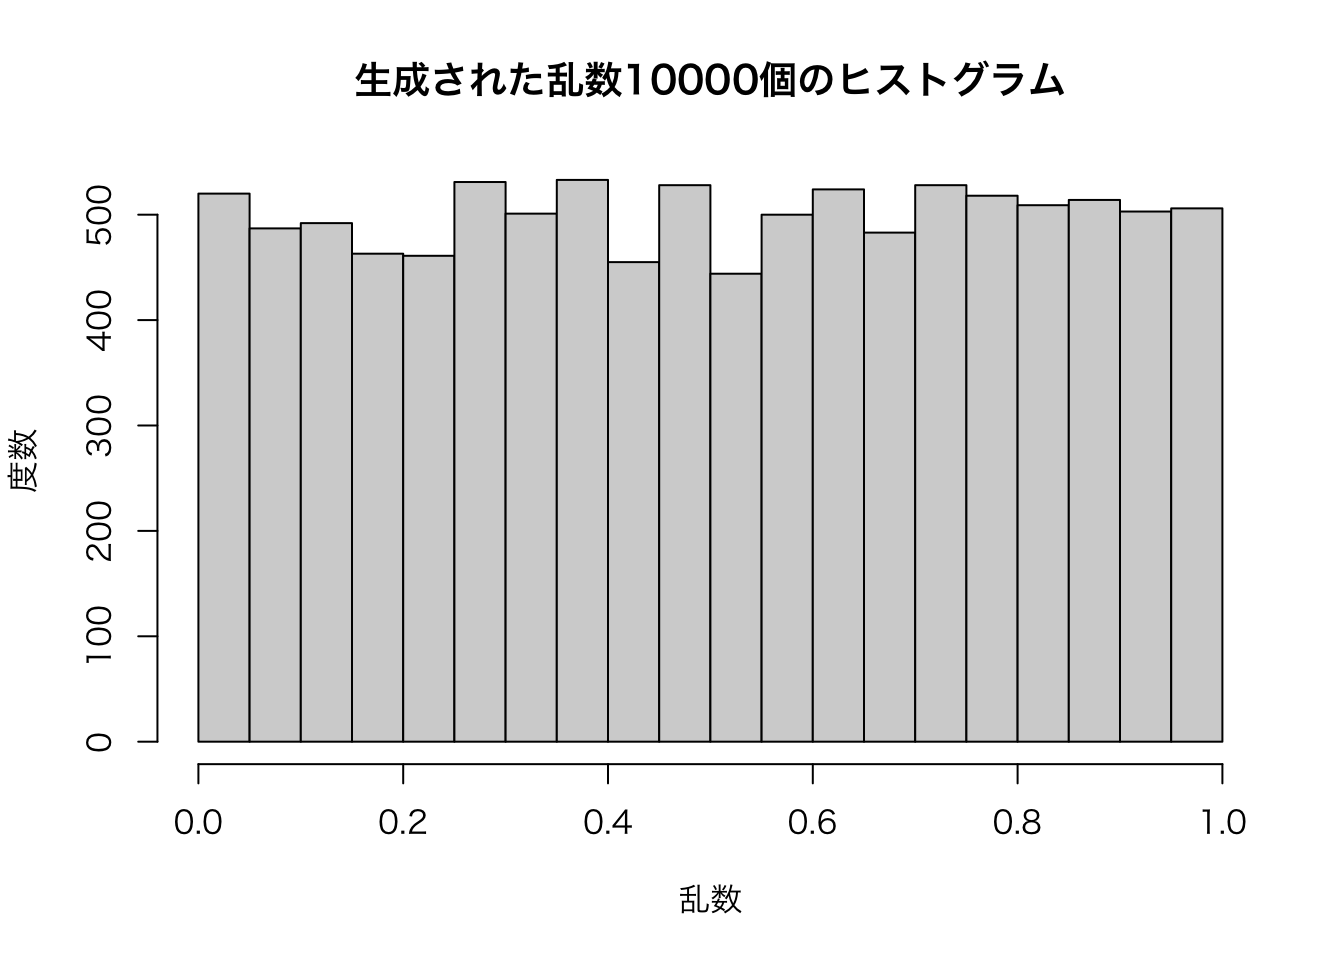
\includegraphics{./factor_files/figure-pdf/unnamed-chunk-87-1.png}

}

\end{figure}

これで図がさらに読みやすくなりました。ちなみに、\texttt{forcats}パッケージは\texttt{last2()}以外にも\texttt{first2()}という関数も提供しております。これを使うと、7月1日でなく、6月27日の新規感染者数の降順で水準の順番が調整されます。他にも引数を2つ使用する自作関数も使えますが、\texttt{fct\_reorder2()}の主な使いみちは\texttt{last2()}で十分でしょう。

\hypertarget{fct_collapse-ux6c34ux6e96ux3092ux7d71ux5408ux3059ux308b}{%
\subsection{\texorpdfstring{\texttt{fct\_collapse()}:
水準を統合する}{fct\_collapse(): 水準を統合する}}\label{fct_collapse-ux6c34ux6e96ux3092ux7d71ux5408ux3059ux308b}}

水準数をより水準数に減らすためには、\texttt{fct\_recode()}を使います。先ほど、\texttt{fct\_shift()}で使った\texttt{df4}の例を考えてみましょう。\texttt{df4}の\texttt{Q1}の水準数は6つです。

\begin{Shaded}
\begin{Highlighting}[numbers=left,,]
\FunctionTok{levels}\NormalTok{(df4}\SpecialCharTok{$}\NormalTok{Q1)}
\end{Highlighting}
\end{Shaded}

\begin{verbatim}
[1] "そう思う"                     "どちらかと言えばそう思う"    
[3] "どちらとも言えない"           "どちらかと言えばそう思わない"
[5] "そう思わない"                 "答えたくない"                
\end{verbatim}

これを4つに減らして見ましょう。具体的には「そう思う」と「どちらかと言えばそう思う」を「そう思う」に、「そう思わない」と「どちらかと言えばそう思わない」を「そう思わない」に統合します。これを\texttt{fct\_recode()}で処理したのが以下のコードです。

\begin{Shaded}
\begin{Highlighting}[numbers=left,,]
\CommentTok{\# fct\_recode()を使った例}
\NormalTok{df4 }\OtherTok{\textless{}{-}}\NormalTok{ df4 }\SpecialCharTok{\%\textgreater{}\%} 
    \FunctionTok{mutate}\NormalTok{(}\AttributeTok{Q1\_R2 =} \FunctionTok{fct\_recode}\NormalTok{(Q1,}
\NormalTok{                              そう思う          }\OtherTok{=} \StringTok{"そう思う"}\NormalTok{,}
\NormalTok{                              そう思う          }\OtherTok{=} \StringTok{"どちらかと言えばそう思う"}\NormalTok{,}
\NormalTok{                              どちらとも言えない  }\OtherTok{=} \StringTok{"どちらとも言えない"}\NormalTok{,}
\NormalTok{                              そう思わない       }\OtherTok{=} \StringTok{"どちらかと言えばそう思わない"}\NormalTok{,}
\NormalTok{                              そう思わない       }\OtherTok{=} \StringTok{"そう思わない"}\NormalTok{,}
\NormalTok{                              答えたくない       }\OtherTok{=} \StringTok{"答えたくない"}\NormalTok{))}

\NormalTok{df4}
\end{Highlighting}
\end{Shaded}

\begin{verbatim}
# A tibble: 10 x 4
      ID Q1                           Q1_R                         Q1_R2        
   <int> <fct>                        <fct>                        <fct>        
 1     1 そう思う                     そう思う                     そう思う     
 2     2 そう思わない                 そう思わない                 そう思わない 
 3     3 どちらとも言えない           どちらとも言えない           どちらとも言~
 4     4 どちらかと言えばそう思う     どちらかと言えばそう思う     そう思う     
 5     5 答えたくない                 答えたくない                 答えたくない 
 6     6 どちらかと言えばそう思う     どちらかと言えばそう思う     そう思う     
 7     7 どちらかと言えばそう思わない どちらかと言えばそう思わない そう思わない 
 8     8 答えたくない                 答えたくない                 答えたくない 
 9     9 そう思わない                 そう思わない                 そう思わない 
10    10 そう思う                     そう思う                     そう思う     
\end{verbatim}

\begin{Shaded}
\begin{Highlighting}[numbers=left,,]
\FunctionTok{levels}\NormalTok{(df4}\SpecialCharTok{$}\NormalTok{Q1\_R2)}
\end{Highlighting}
\end{Shaded}

\begin{verbatim}
[1] "そう思う"           "どちらとも言えない" "そう思わない"      
[4] "答えたくない"      
\end{verbatim}

しかし、水準を統合するに特化した\texttt{fct\_collapse()}を使えばより便利です。使い方は、\texttt{fct\_recode()}に非常に似ているため省略しますが、\texttt{=}の右側を\texttt{c()}でまとめることが出来ます。

\begin{Shaded}
\begin{Highlighting}[numbers=left,,]
\CommentTok{\# fct\_collapse()を使った例}
\NormalTok{df4 }\OtherTok{\textless{}{-}}\NormalTok{ df4 }\SpecialCharTok{\%\textgreater{}\%} 
    \FunctionTok{mutate}\NormalTok{(}\AttributeTok{Q1\_R3 =} \FunctionTok{fct\_collapse}\NormalTok{(Q1,}
\NormalTok{                                そう思う }\OtherTok{=} \FunctionTok{c}\NormalTok{(}\StringTok{"そう思う"}\NormalTok{, }\StringTok{"どちらかと言えばそう思う"}\NormalTok{),}
\NormalTok{                                どちらとも言えない }\OtherTok{=} \StringTok{"どちらとも言えない"}\NormalTok{,}
\NormalTok{                                そう思わない }\OtherTok{=} \FunctionTok{c}\NormalTok{( }\StringTok{"どちらかと言えばそう思わない"}\NormalTok{, }\StringTok{"そう思わない"}\NormalTok{),}
\NormalTok{                                答えたくない }\OtherTok{=} \StringTok{"答えたくない"}\NormalTok{))}

\NormalTok{df4}
\end{Highlighting}
\end{Shaded}

\begin{verbatim}
# A tibble: 10 x 5
      ID Q1                           Q1_R                         Q1_R2   Q1_R3
   <int> <fct>                        <fct>                        <fct>   <fct>
 1     1 そう思う                     そう思う                     そう思~ そう~
 2     2 そう思わない                 そう思わない                 そう思~ そう~
 3     3 どちらとも言えない           どちらとも言えない           どちら~ どち~
 4     4 どちらかと言えばそう思う     どちらかと言えばそう思う     そう思~ そう~
 5     5 答えたくない                 答えたくない                 答えた~ 答え~
 6     6 どちらかと言えばそう思う     どちらかと言えばそう思う     そう思~ そう~
 7     7 どちらかと言えばそう思わない どちらかと言えばそう思わない そう思~ そう~
 8     8 答えたくない                 答えたくない                 答えた~ 答え~
 9     9 そう思わない                 そう思わない                 そう思~ そう~
10    10 そう思う                     そう思う                     そう思~ そう~
\end{verbatim}

\begin{Shaded}
\begin{Highlighting}[numbers=left,,]
\FunctionTok{levels}\NormalTok{(df4}\SpecialCharTok{$}\NormalTok{Q1\_R3)}
\end{Highlighting}
\end{Shaded}

\begin{verbatim}
[1] "そう思う"           "どちらとも言えない" "そう思わない"      
[4] "答えたくない"      
\end{verbatim}

\texttt{fct\_recode()}の結果と同じ結果が得られました。元の水準数や、減らされる水準数などによっては書く手間があまり変わらないので、好きな方を使っても良いでしょう。

\hypertarget{fct_drop-ux4f7fux308fux308cux3066ux3044ux306aux3044ux6c34ux6e96ux3092ux9664ux53bbux3059ux308b}{%
\subsection{\texorpdfstring{\texttt{fct\_drop()}:
使われていない水準を除去する}{fct\_drop(): 使われていない水準を除去する}}\label{fct_drop-ux4f7fux308fux308cux3066ux3044ux306aux3044ux6c34ux6e96ux3092ux9664ux53bbux3059ux308b}}

水準としては存在するものの、データとしては存在しないケースもあります。これをここでは「空水準
(empty
levels)」と呼びます。たとえば、以下のコードは\texttt{Pref}をfactor化してから\texttt{Pref\ ==\ "奈良県"}のケースを落としたものです。

\begin{Shaded}
\begin{Highlighting}[numbers=left,,]
\NormalTok{Score\_df\_f2 }\OtherTok{\textless{}{-}}\NormalTok{ df }\SpecialCharTok{\%\textgreater{}\%}
  \FunctionTok{mutate}\NormalTok{(}\AttributeTok{Pref =} \FunctionTok{fct\_inorder}\NormalTok{(Pref)) }\SpecialCharTok{\%\textgreater{}\%}
  \FunctionTok{filter}\NormalTok{(Pref }\SpecialCharTok{!=} \StringTok{"奈良県"}\NormalTok{) }\SpecialCharTok{\%\textgreater{}\%}
  \FunctionTok{group\_by}\NormalTok{(Pref) }\SpecialCharTok{\%\textgreater{}\%}
  \FunctionTok{summarise}\NormalTok{(}\AttributeTok{Score   =} \FunctionTok{mean}\NormalTok{(Score, }\AttributeTok{na.rm =} \ConstantTok{TRUE}\NormalTok{),}
            \AttributeTok{.groups =} \StringTok{"drop"}\NormalTok{)}

\NormalTok{Score\_df\_f2}
\end{Highlighting}
\end{Shaded}

\begin{verbatim}
# A tibble: 8 x 2
  Pref     Score
  <fct>    <dbl>
1 東京都    3.67
2 神奈川県  3.53
3 千葉県    3.72
4 埼玉県    3.64
5 大阪府    3.77
6 京都府    3.68
7 兵庫県    3.54
8 和歌山県  3.97
\end{verbatim}

このように結果としては、奈良県のデータを除外したため空水準である奈良県は表示されませんが、\texttt{Pref}変数はどうでしょうか。

\begin{Shaded}
\begin{Highlighting}[numbers=left,,]
\FunctionTok{levels}\NormalTok{(Score\_df\_f2}\SpecialCharTok{$}\NormalTok{Pref)}
\end{Highlighting}
\end{Shaded}

\begin{verbatim}
[1] "東京都"   "神奈川県" "千葉県"   "埼玉県"   "大阪府"   "京都府"   "兵庫県"  
[8] "奈良県"   "和歌山県"
\end{verbatim}

このように水準としては残っていることが分かります。使われていない水準が分析や可視化に影響を与えないケースもありますが、与えるケースもあります。これもこれまで勉強してきた\texttt{fct\_*()}関数群で対応可能ですが、\texttt{fct\_drop()}関数を使えば一発で終わります。実際にやってみましょう。

\begin{Shaded}
\begin{Highlighting}[numbers=left,,]
\NormalTok{Score\_df\_f2 }\OtherTok{\textless{}{-}}\NormalTok{ Score\_df\_f2 }\SpecialCharTok{\%\textgreater{}\%}
  \FunctionTok{mutate}\NormalTok{(}\AttributeTok{Pref =} \FunctionTok{fct\_drop}\NormalTok{(Pref))}
\end{Highlighting}
\end{Shaded}

\begin{Shaded}
\begin{Highlighting}[numbers=left,,]
\FunctionTok{levels}\NormalTok{(Score\_df\_f2}\SpecialCharTok{$}\NormalTok{Pref)}
\end{Highlighting}
\end{Shaded}

\begin{verbatim}
[1] "東京都"   "神奈川県" "千葉県"   "埼玉県"   "大阪府"   "京都府"   "兵庫県"  
[8] "和歌山県"
\end{verbatim}

水準から奈良県が消えました。同じ機能をする関数としてはR内蔵関数である\texttt{droplevels()}関数があり、使い方は\texttt{fct\_drop()}と同じです。

\hypertarget{fct_expand-ux6c34ux6e96ux3092ux8ffdux52a0ux3059ux308b}{%
\subsection{\texorpdfstring{\texttt{fct\_expand()}:
水準を追加する}{fct\_expand(): 水準を追加する}}\label{fct_expand-ux6c34ux6e96ux3092ux8ffdux52a0ux3059ux308b}}

一方、空水準を追加することも可能です。\texttt{fct\_expand()}関数には元の変数名に加え、追加する水準名を入れるだけです。たとえば、\texttt{df}の\texttt{Pref}の水準は関東と関西の9都府県名となっていますが、ここに\texttt{"滋賀県"}という水準を追加してみます。。

\begin{Shaded}
\begin{Highlighting}[numbers=left,,]
\NormalTok{df5 }\OtherTok{\textless{}{-}}\NormalTok{ df }\SpecialCharTok{\%\textgreater{}\%}
  \FunctionTok{mutate}\NormalTok{(}\AttributeTok{Pref =} \FunctionTok{fct\_expand}\NormalTok{(Pref, }\StringTok{"滋賀県"}\NormalTok{))}

\FunctionTok{levels}\NormalTok{(df5}\SpecialCharTok{$}\NormalTok{Pref)}
\end{Highlighting}
\end{Shaded}

\begin{verbatim}
 [1] "京都府"   "兵庫県"   "千葉県"   "和歌山県" "埼玉県"   "大阪府"  
 [7] "奈良県"   "東京都"   "神奈川県" "滋賀県"  
\end{verbatim}

\texttt{"滋賀県"}という新しい水準が出来ましたね。ただし、新しく追加された水準は最後の順番になりますので、修正が必要な場合は\texttt{fct\_relevel()}などを使って適宜修正してください。

新しく水準が追加されることによって、何かの変化はあるでしょうか。まずは都府県ごとに\texttt{Score}の平均値とケース数を計算してみましょう。

\begin{Shaded}
\begin{Highlighting}[numbers=left,,]
\NormalTok{df5 }\SpecialCharTok{\%\textgreater{}\%}
  \FunctionTok{group\_by}\NormalTok{(Pref) }\SpecialCharTok{\%\textgreater{}\%}
  \FunctionTok{summarise}\NormalTok{(}\AttributeTok{Score   =} \FunctionTok{mean}\NormalTok{(Score, }\AttributeTok{na.rm =} \ConstantTok{TRUE}\NormalTok{),}
            \AttributeTok{N       =} \FunctionTok{n}\NormalTok{(),}
            \AttributeTok{.groups =} \StringTok{"drop"}\NormalTok{)}
\end{Highlighting}
\end{Shaded}

\begin{verbatim}
# A tibble: 9 x 3
  Pref     Score     N
  <fct>    <dbl> <int>
1 京都府    3.68   414
2 兵庫県    3.54   591
3 千葉県    3.72  1000
4 和歌山県  3.97   140
5 埼玉県    3.64  1000
6 大阪府    3.77  1000
7 奈良県    3.85   147
8 東京都    3.67  1000
9 神奈川県  3.53  1000
\end{verbatim}

見た目は全く変わらず、滋賀県の行が新しく出来たわけでもありません。\texttt{dplyr}の\texttt{group\_by()}の場合、空水準はグループ化の対象になりません。一方、多くのR内蔵関数はケースとして存在しなくても計算の対象となります。たとえば、ベクトル内のある値が何個格納されているか確認する\texttt{table()}関数の例を見てみましょう。

\begin{Shaded}
\begin{Highlighting}[numbers=left,,]
\FunctionTok{table}\NormalTok{(df5}\SpecialCharTok{$}\NormalTok{Pref)}
\end{Highlighting}
\end{Shaded}

\begin{verbatim}
  京都府   兵庫県   千葉県 和歌山県   埼玉県   大阪府   奈良県   東京都 
     414      591     1000      140     1000     1000      147     1000 
神奈川県   滋賀県 
    1000        0 
\end{verbatim}

\texttt{"滋賀県"}という列があり、合致するケースが0と表示されます。\texttt{group\_by()}でも空の水準まで含めて出力する引数\texttt{.drop}があります。デフォルトは\texttt{TRUE}ですが、これを\texttt{FALSE}に指定してみます。

\begin{Shaded}
\begin{Highlighting}[numbers=left,,]
\NormalTok{df5 }\SpecialCharTok{\%\textgreater{}\%}
  \FunctionTok{group\_by}\NormalTok{(Pref, }\AttributeTok{.drop =} \ConstantTok{FALSE}\NormalTok{) }\SpecialCharTok{\%\textgreater{}\%}
  \FunctionTok{summarise}\NormalTok{(}\AttributeTok{Score   =} \FunctionTok{mean}\NormalTok{(Score, }\AttributeTok{na.rm =} \ConstantTok{TRUE}\NormalTok{),}
            \AttributeTok{N       =} \FunctionTok{n}\NormalTok{(),}
            \AttributeTok{.groups =} \StringTok{"drop"}\NormalTok{)}
\end{Highlighting}
\end{Shaded}

\begin{verbatim}
# A tibble: 10 x 3
   Pref      Score     N
   <fct>     <dbl> <int>
 1 京都府     3.68   414
 2 兵庫県     3.54   591
 3 千葉県     3.72  1000
 4 和歌山県   3.97   140
 5 埼玉県     3.64  1000
 6 大阪府     3.77  1000
 7 奈良県     3.85   147
 8 東京都     3.67  1000
 9 神奈川県   3.53  1000
10 滋賀県   NaN        0
\end{verbatim}

空水準も出力され、\texttt{Score}の平均値は計算不可
(\texttt{NaN})、ケース数は0という結果が得られました。

\hypertarget{fct_explicit_na-ux6b20ux640dux5024ux306bux6c34ux6e96ux3092ux4e0eux3048ux308b}{%
\subsection{\texorpdfstring{\texttt{fct\_explicit\_na()}:
欠損値に水準を与える}{fct\_explicit\_na(): 欠損値に水準を与える}}\label{fct_explicit_na-ux6b20ux640dux5024ux306bux6c34ux6e96ux3092ux4e0eux3048ux308b}}

まずは、実習用データ\texttt{df6}を作ってみまます。\texttt{X1}はnumeric型変数ですが、これをfactor化します。最初から\texttt{tibble()}内でfactor化しておいても問題ありませんが、練習だと思ってください。

\begin{Shaded}
\begin{Highlighting}[numbers=left,,]
\NormalTok{df6 }\OtherTok{\textless{}{-}} \FunctionTok{tibble}\NormalTok{(}
  \AttributeTok{ID =} \DecValTok{1}\SpecialCharTok{:}\DecValTok{10}\NormalTok{,}
  \AttributeTok{X1 =} \FunctionTok{c}\NormalTok{(}\DecValTok{1}\NormalTok{, }\DecValTok{3}\NormalTok{, }\DecValTok{2}\NormalTok{, }\ConstantTok{NA}\NormalTok{, }\DecValTok{2}\NormalTok{, }\DecValTok{2}\NormalTok{, }\DecValTok{1}\NormalTok{, }\ConstantTok{NA}\NormalTok{, }\DecValTok{3}\NormalTok{, }\ConstantTok{NA}\NormalTok{)}
\NormalTok{)}

\NormalTok{df6 }\OtherTok{\textless{}{-}}\NormalTok{ df6 }\SpecialCharTok{\%\textgreater{}\%}
  \FunctionTok{mutate}\NormalTok{(}\AttributeTok{X1 =} \FunctionTok{factor}\NormalTok{(X1, }
                     \AttributeTok{levels =} \FunctionTok{c}\NormalTok{(}\DecValTok{1}\NormalTok{, }\DecValTok{2}\NormalTok{, }\DecValTok{3}\NormalTok{),}
                     \AttributeTok{labels =} \FunctionTok{c}\NormalTok{(}\StringTok{"ラーメン"}\NormalTok{, }\StringTok{"うどん"}\NormalTok{, }\StringTok{"そば"}\NormalTok{)))}

\NormalTok{df6}
\end{Highlighting}
\end{Shaded}

\begin{verbatim}
# A tibble: 10 x 2
      ID X1      
   <int> <fct>   
 1     1 ラーメン
 2     2 そば    
 3     3 うどん  
 4     4 <NA>    
 5     5 うどん  
 6     6 うどん  
 7     7 ラーメン
 8     8 <NA>    
 9     9 そば    
10    10 <NA>    
\end{verbatim}

それでは\texttt{X1}をグループ化変数とし、ケース数を計算してみましょう。

\begin{Shaded}
\begin{Highlighting}[numbers=left,,]
\NormalTok{df6 }\SpecialCharTok{\%\textgreater{}\%}
  \FunctionTok{group\_by}\NormalTok{(X1) }\SpecialCharTok{\%\textgreater{}\%}
  \FunctionTok{summarise}\NormalTok{(}\AttributeTok{N       =} \FunctionTok{n}\NormalTok{(),}
            \AttributeTok{.groups =} \StringTok{"drop"}\NormalTok{)}
\end{Highlighting}
\end{Shaded}

\begin{verbatim}
# A tibble: 4 x 2
  X1           N
  <fct>    <int>
1 ラーメン     2
2 うどん       3
3 そば         2
4 <NA>         3
\end{verbatim}

\texttt{NA}もグループ化の対象となります。以下はこの欠損値も一つの水準として指定する方法について紹介します。欠損値を欠損値のままにするケースが多いですが、欠損値が何らかの意味を持つ場合、分析の対象になります。たとえば、多項ロジスティック回帰の応答変数として「分からない/答えたくない」を含めたり、\href{https://ci.nii.ac.jp/naid/40021269699}{「分からない/答えたくない」を選択する要因を分析}したい場合は、欠損値に値を与える必要があります。なぜなら、一般的な分析において欠損値は分析対象から除外されるからです。

まずは、これまで紹介した関数を使ったやり方から紹介します。

\begin{Shaded}
\begin{Highlighting}[numbers=left,,]
\NormalTok{df6 }\SpecialCharTok{\%\textgreater{}\%}
         \CommentTok{\# まず、X1をcharacter型に変換し、X2という列に保存}
  \FunctionTok{mutate}\NormalTok{(}\AttributeTok{X2 =} \FunctionTok{as.character}\NormalTok{(X1),}
         \CommentTok{\# X2がNAなら"欠損値"、それ以外なら元のX2の値に置換}
         \AttributeTok{X2 =} \FunctionTok{ifelse}\NormalTok{(}\FunctionTok{is.na}\NormalTok{(X2), }\StringTok{"欠損値"}\NormalTok{, X2),}
         \CommentTok{\# X2を再度factor化する}
         \AttributeTok{X2 =} \FunctionTok{factor}\NormalTok{(X2, }
                     \AttributeTok{levels =} \FunctionTok{c}\NormalTok{(}\StringTok{"ラーメン"}\NormalTok{, }\StringTok{"うどん"}\NormalTok{, }\StringTok{"そば"}\NormalTok{, }\StringTok{"欠損値"}\NormalTok{)))}
\end{Highlighting}
\end{Shaded}

\begin{verbatim}
# A tibble: 10 x 3
      ID X1       X2      
   <int> <fct>    <fct>   
 1     1 ラーメン ラーメン
 2     2 そば     そば    
 3     3 うどん   うどん  
 4     4 <NA>     欠損値  
 5     5 うどん   うどん  
 6     6 うどん   うどん  
 7     7 ラーメン ラーメン
 8     8 <NA>     欠損値  
 9     9 そば     そば    
10    10 <NA>     欠損値  
\end{verbatim}

\texttt{X1}をcharacter型に戻す理由\footnote{character型でなく、numeric型でも出来ます。}は、水準にない値が入るとfactor化が解除されるからです。factor型をcharacter型に戻さずに\texttt{df6\$X1}の\texttt{NA}を\texttt{"欠損値"}に置換すると、以下のようになります。

\begin{Shaded}
\begin{Highlighting}[numbers=left,,]
\CommentTok{\# df6のX1がNAなら"欠損"、それ以外なら元のX1の値を返す}
\FunctionTok{ifelse}\NormalTok{(}\FunctionTok{is.na}\NormalTok{(df6}\SpecialCharTok{$}\NormalTok{X1), }\StringTok{"欠損値"}\NormalTok{, df6}\SpecialCharTok{$}\NormalTok{X1)}
\end{Highlighting}
\end{Shaded}

\begin{verbatim}
 [1] "1"      "3"      "2"      "欠損値" "2"      "2"      "1"      "欠損値"
 [9] "3"      "欠損値"
\end{verbatim}

\texttt{"ラーメン"}と\texttt{"うどん"}、\texttt{"そば"}がfactor化前の1,
2,
3に戻っただけでなく、\texttt{NA}が\texttt{"欠損値"}というcharacter型に置換されたため、全体がcharacter型に変換されました。このように欠損値に水準を与える作業は難しくはありませんが、面倒な作業です。そこで登場する関数が\texttt{fct\_exlpicit\_na()}関数です。使い方は、元の変数に加え、欠損値の水準名を指定する\texttt{na\_level}です。

\begin{Shaded}
\begin{Highlighting}[numbers=left,,]
\NormalTok{df6 }\OtherTok{\textless{}{-}}\NormalTok{ df6 }\SpecialCharTok{\%\textgreater{}\%}
  \CommentTok{\# na\_levelのデフォルト値は"(Missing)"}
  \FunctionTok{mutate}\NormalTok{(}\AttributeTok{X2 =} \FunctionTok{fct\_explicit\_na}\NormalTok{(X1, }\AttributeTok{na\_level =} \StringTok{"欠損値"}\NormalTok{))}

\NormalTok{df6}
\end{Highlighting}
\end{Shaded}

\begin{verbatim}
# A tibble: 10 x 3
      ID X1       X2      
   <int> <fct>    <fct>   
 1     1 ラーメン ラーメン
 2     2 そば     そば    
 3     3 うどん   うどん  
 4     4 <NA>     欠損値  
 5     5 うどん   うどん  
 6     6 うどん   うどん  
 7     7 ラーメン ラーメン
 8     8 <NA>     欠損値  
 9     9 そば     そば    
10    10 <NA>     欠損値  
\end{verbatim}

欠損値が一つの水準になったことが分かります。

\begin{Shaded}
\begin{Highlighting}[numbers=left,,]
\NormalTok{df6 }\SpecialCharTok{\%\textgreater{}\%}
  \FunctionTok{group\_by}\NormalTok{(X2) }\SpecialCharTok{\%\textgreater{}\%}
  \FunctionTok{summarise}\NormalTok{(}\AttributeTok{N       =} \FunctionTok{n}\NormalTok{(),}
            \AttributeTok{.groups =} \StringTok{"drop"}\NormalTok{)}
\end{Highlighting}
\end{Shaded}

\begin{verbatim}
# A tibble: 4 x 2
  X2           N
  <fct>    <int>
1 ラーメン     2
2 うどん       3
3 そば         2
4 欠損値       3
\end{verbatim}

むろん、\texttt{group\_by()}を使ってもちゃんと出力されます。

\hypertarget{sec-tidydata}{%
\chapter{整然データ構造}\label{sec-tidydata}}

本章ではグラフの作成に適した形へデータを整形することについて学習します。ただし、これはグラフに限られた話ではありません。作図に適したデータは分析にも適します。

\hypertarget{sec-tidydata_intro}{%
\section{整然データ (tidy data)とは}\label{sec-tidydata_intro}}

分析や作図に適したデータの形は整然データ、または簡潔データ (tidy
data)と呼ばれます。整然データの概念はtidyverse世界の産みの親であるHadely
Wickham先生が提唱した概念であり、詳細は \citet{Wickham:2014}
を参照してください。

整然データは目指す到達点は非常に単純です。それは「データの構造
(structure)と意味
(semantic)を一致させる」ことです。そして、この「意味」を出来る限り小さい単位で分解します。

例えば、3人で構成されたあるクラス内の被験者に対し、投薬前後に測定した数学成績があるとします。投薬前の成績は\texttt{"Control"}、投薬後の状況を\texttt{"Treatment"}とします。これをまとめたのが
表~\ref{tbl-tidydata_messy_data1} です。

\hypertarget{tbl-tidydata_messy_data1}{}
\begin{table}
\caption{\label{tbl-tidydata_messy_data1}Messy Dataの例 (1) }

\centering
\begin{tabular}{lrr}
\toprule
\multicolumn{1}{c}{Name} & \multicolumn{1}{c}{Control} & \multicolumn{1}{c}{Treatment}\\
\midrule
Hadley & 90 & 90\\
Song & 80 & 25\\
Yanai & 100 & 95\\
\bottomrule
\end{tabular}
\end{table}

また、以上の表は転置も可能であり、以下のように表現することが可能です (
表~\ref{tbl-tidydata_messy_data2} )。

\hypertarget{tbl-tidydata_messy_data2}{}
\begin{table}
\caption{\label{tbl-tidydata_messy_data2}Messy Dataの例 (2) }

\centering
\begin{tabular}{lrrr}
\toprule
\multicolumn{1}{c}{Treat} & \multicolumn{1}{c}{Hadely} & \multicolumn{1}{c}{Song} & \multicolumn{1}{c}{Yanai}\\
\midrule
Control & 90 & 80 & 100\\
Treatment & 90 & 25 & 95\\
\bottomrule
\end{tabular}
\end{table}

2つのデータが持つ情報は全く同じです。これは「同じ意味を持つが、異なる構造を持つ」とも言えます。このような多様性が生じる理由は行と列のあり方が各値を説明するに十分ではないからです。異なるデータ構造として表現される余地があるということです。

たとえば、 表~\ref{tbl-tidydata_tidydata}
の場合、各列は以下のような3つの情報があります。

\begin{enumerate}
\def\labelenumi{\arabic{enumi}.}
\tightlist
\item
  \texttt{Name}: 被験者名
\item
  \texttt{Control}: \textbf{投薬前}の\textbf{数学成績}
\item
  \texttt{Treatment}: \textbf{投薬後}の\textbf{数学成績}
\end{enumerate}

このデータの問題は「投薬有無」と「数学成績」が2回登場したという点です。1は問題ありませんが、2と3の値は「投薬有無
\(\times\)
数学成績」の組み合わせです。一つの変数に2つの情報が含まれていますね。これによって、投薬有無を行にしても列にしてもいいわけです。「ならばこっちの方が柔軟だしいいのでは?」と思う方もいるかも知れません。しかし、パソコンはこの曖昧さが嫌いです。なぜなら、人間のような思考ができないからです。データフレームは縦ベクトルの集合であるから、各列には一つの情報のみ格納する必要があります。たとえば、以下のように列を変更するとしましょう。

\begin{enumerate}
\def\labelenumi{\arabic{enumi}.}
\tightlist
\item
  \texttt{Name}: 被験者名
\item
  \texttt{Treat}: 投薬有無
\item
  \texttt{Math\_Score}: 数学成績
\end{enumerate}

\texttt{Treat}は投薬前なら\texttt{"Control"}の値を、投薬後なら\texttt{"Treatment"}の値が入ります。\texttt{Math\_Socre}には数学成績が入ります。これに則って表に直したのが
表~\ref{tbl-tidydata_tidydata} です。

\hypertarget{tbl-tidydata_tidydata}{}
\begin{table}
\caption{\label{tbl-tidydata_tidydata}整然データの例 }

\centering
\begin{tabular}{l|l|r}
\hline
\multicolumn{1}{c}{Name} & \multicolumn{1}{c}{Treat} & \multicolumn{1}{c}{Math\_Score}\\
\hline
Hadley & Control & 90\\
\hline
Hadley & Treatment & 90\\
\hline
Song & Control & 80\\
\hline
Song & Treatment & 25\\
\hline
Yanai & Control & 100\\
\hline
Yanai & Treatment & 95\\
\hline
\end{tabular}
\end{table}

表が長くなりましたが、これなら一つの列に2つ以上の情報が含まれることはありません。この場合、
表~\ref{tbl-tidydata_messy_data1} と 表~\ref{tbl-tidydata_messy_data2}
のように、行と列を転置することができるでしょうか。

\hypertarget{tbl-tidydata_transdata}{}
\begin{table}
\caption{\label{tbl-tidydata_transdata}整然データを転置した場合 }

\centering
\begin{tabular}{l|l|l|l|l|l|l}
\hline
\multicolumn{1}{c}{Name} & \multicolumn{1}{c}{Hadley} & \multicolumn{1}{c}{Hadley} & \multicolumn{1}{c}{Song} & \multicolumn{1}{c}{Song} & \multicolumn{1}{c}{Yanai} & \multicolumn{1}{c}{Yanai}\\
\hline
Treat & Control & Treatment & Control & Treatment & Control & Treatment\\
\hline
Math\_Score & 90 & 90 & 80 & 25 & 100 & 95\\
\hline
\end{tabular}
\end{table}

その結果が 表~\ref{tbl-tidydata_transdata}
ですが、いかがでしょうか。まず、列名が重複している時点でアウトですし、人間が見ても非常に分かりにくい表になりました。また、一つの列に異なるデータ
(この場合、character型とnumeirc型)が混在しています。パソコンから見てはわけのわからないデータになったわけです。

ここまで来たら整然データのイメージはある程度掴めたかも知れません。具体的に整然データとは次の4つの条件を満たすデータです\citep{Wickham:2014}。

\begin{enumerate}
\def\labelenumi{\arabic{enumi}.}
\tightlist
\item
  1つの列は、1つの変数を表す。
\item
  1つの行は、1つの観測を表す。
\item
  1つのセル(特定の列の特定の行)は、1つの値を表す。
\item
  1つの表は、1つの観測単位 (unit of
  observation)をもつ(異なる観測単位が混ざっていない)。
\end{enumerate}

以下でも、 表~\ref{tbl-tidydata_messy_data1} と
表~\ref{tbl-tidydata_tidydata}
を対比しながら、以上の4条件をより詳しく説明します。

\hypertarget{ux3064ux306eux5217ux306f1ux3064ux306eux5909ux6570ux3092ux8868ux3059}{%
\subsection{1つの列は、1つの変数を表す}\label{ux3064ux306eux5217ux306f1ux3064ux306eux5909ux6570ux3092ux8868ux3059}}

表~\ref{tbl-tidydata_messy_data1} と 表~\ref{tbl-tidydata_tidydata}
に含まれる情報は以下の3つで共通しています。

\begin{enumerate}
\def\labelenumi{\arabic{enumi}.}
\tightlist
\item
  被験者名
\item
  投薬有無
\item
  数学成績
\end{enumerate}

これらの情報がそれぞれデータの変数になるわけですが、整然データは一つの列が一つの変数を表します。それではまず、
表~\ref{tbl-tidydata_messy_data1} ( 図~\ref{fig-tidydata_example1}
の左)から考えてみましょう。この図には3つの情報が全て含まれています。しかし、数学成績は2列に渡って格納されており、「1列1変数」の条件を満たしておりません。一方、
表~\ref{tbl-tidydata_messy_data1} ( 図~\ref{fig-tidydata_example1}
の右)は投薬前後を表す\texttt{Treat}変数を作成し、その値に応じた数学成績が格納されており、「1列1変数」の条件を満たしています。

\begin{figure}

{\centering 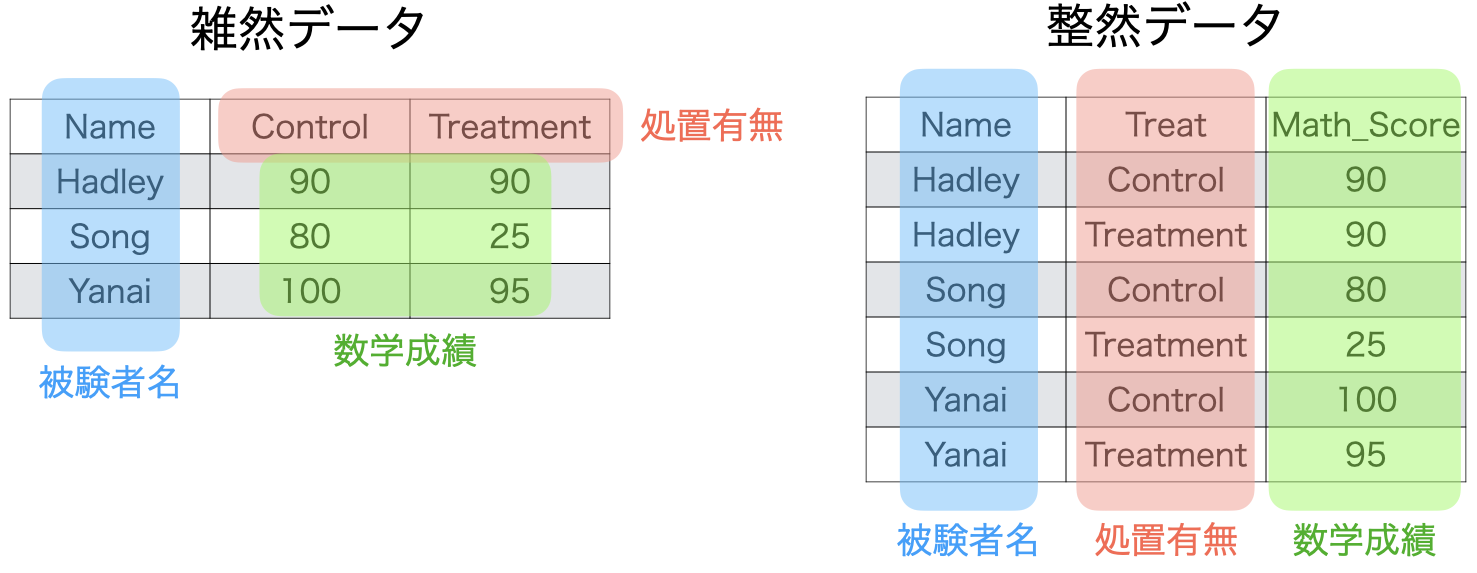
\includegraphics[width=0.5\textwidth,height=\textheight]{./Figs/Tidydata/TidyData1.png}

}

\caption{\label{fig-tidydata_example1}1つの列は、1つの変数を表す}

\end{figure}

「1列1変数」は整然データの最も基本となる条件であり、整然データ作成の出発点とも言えます。

\hypertarget{ux3064ux306eux884cux306f1ux3064ux306eux89b3ux6e2cux3092ux8868ux3059}{%
\subsection{1つの行は、1つの観測を表す}\label{ux3064ux306eux884cux306f1ux3064ux306eux89b3ux6e2cux3092ux8868ux3059}}

図~\ref{fig-tidydata_example2}
の左は一行当たり、いくつの観察が含まれているでしょうか。それを確認するためには、このデータが何を観察しているかを考える必要があります。このデータは投薬\textbf{前後}の数学成績を観察し、量的に測定したものです。つまり、同じ人に対して2回観察を行ったことになります。したがって、投薬前の数学成績と投薬後の数学成績は別の観察であり、
図~\ref{fig-tidydata_example2}
の左は3行の表ですが、実は6回分の観察が含まれていることになります。1行に2つの観察が載っていることですね。

\begin{figure}

{\centering 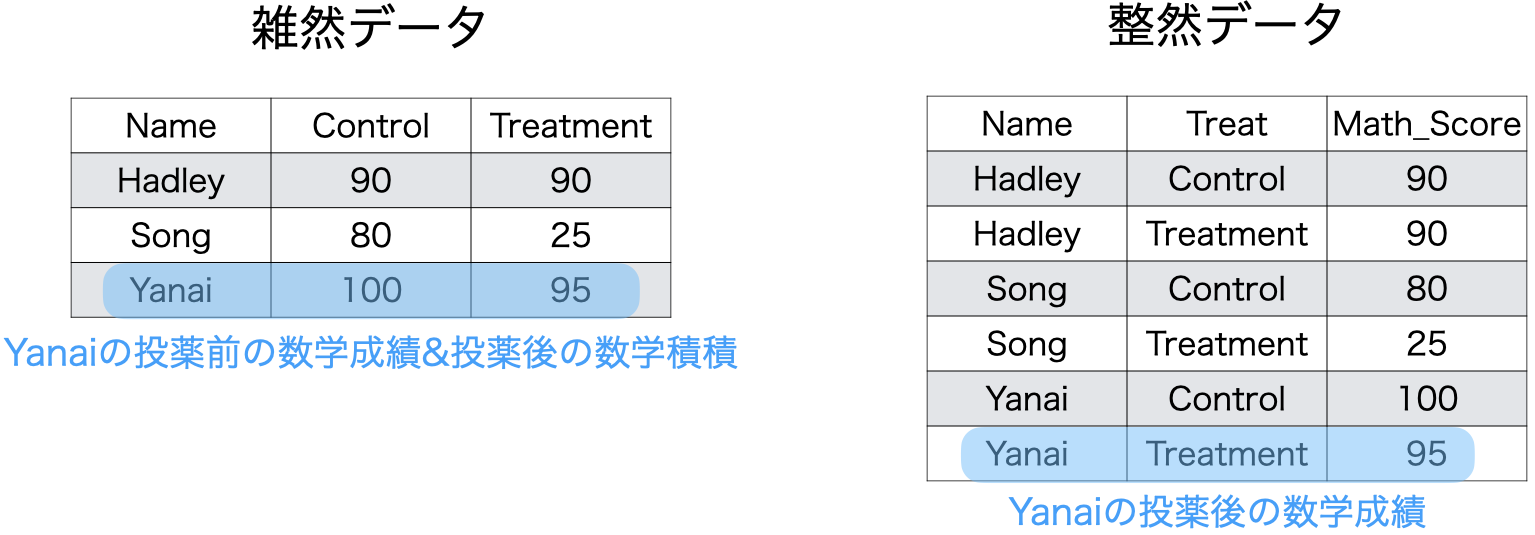
\includegraphics[width=0.5\textwidth,height=\textheight]{./Figs/Tidydata/TidyData2.png}

}

\caption{\label{fig-tidydata_example2}1つの行は、1つの観測を表す}

\end{figure}

一方、 図~\ref{fig-tidydata_example2}
の右は6行のデータであり、観察回数とデータの行数が一致しています。つまり、1行に1観察となります。

今回は数学成績しか測っていたいので、簡単な例ですが、実際のデータには曖昧な部分があります。たとえば、投薬によって血圧が変化する可能性があるため、最高血圧もまた投薬前後に測定したとします。それが
表~\ref{tbl-tidydata_blood} の左です。

\begin{table}

\caption{\label{tbl-tidydata_blood}1行1観察の例}\begin{minipage}[t]{0.50\linewidth}
\subcaption{\label{tbl-tidydata_blood-1}雑然データ }

{\centering 

\raisebox{-\height}{

\centering
\begin{tabular}{llrr}
\toprule
Name & Treat & Math & Blood\\
\midrule
Hadley & Control & 90 & 110\\
Hadley & Treatment & 90 & 115\\
Song & Control & 80 & 95\\
Song & Treatment & 25 & 110\\
Yanai & Control & 100 & 100\\
\addlinespace
Yanai & Treatment & 95 & 95\\
\bottomrule
\end{tabular}

}

}

\end{minipage}%
%
\begin{minipage}[t]{0.50\linewidth}
\subcaption{\label{tbl-tidydata_blood-2}整然データ }

{\centering 

\raisebox{-\height}{

\centering
\begin{tabular}{lllr}
\toprule
Name & Treat & Type & Value\\
\midrule
Hadley & Control & Math & 90\\
Hadley & Control & Blood & 110\\
Hadley & Treatment & Math & 90\\
Hadley & Treatment & Blood & 115\\
Song & Control & Math & 80\\
\addlinespace
Song & Control & Blood & 95\\
Song & Treatment & Math & 25\\
Song & Treatment & Blood & 110\\
Yanai & Control & Math & 100\\
Yanai & Control & Blood & 100\\
\addlinespace
Yanai & Treatment & Math & 95\\
Yanai & Treatment & Blood & 95\\
\bottomrule
\end{tabular}

}

}

\end{minipage}%

\end{table}

3人に投薬前後に数学成績と最高血圧を測定した場合の観察回数は何回でしょう。3人
\(\times\) 2時点 \(\times\)
2指標の測定だから12回の測定でしょうか。ならば、
表~\ref{tbl-tidydata_blood}
の右が整然データでしょう。しかし、この場合、1列1変数という条件が満たされなくなります。\texttt{Value}列には数学成績と血圧が混在しており、2つの変数になります。ならば、どれも整然データではないということでしょうか。実は整然データは
表~\ref{tbl-tidydata_blood}
の左です。なぜなら、「1観察=1値」ではないからです。データにおける観察とは観察単位ごとに測定された\textbf{値の集合}です。観察対象とは人や自治体、企業、国などだけでなく、時間も含まれます。たとえば、人の特徴
(性別、身長、所得、政治関心など)を測定しもの、ある日の特徴
(気温、株価など)を測定したもの全てが観察です。むろん、人 \(\times\)
時間のような組み合わせが観察単位ともなり得ます。この一つ一つの観察単位から得られた値の集合が観察です。
表~\ref{tbl-tidydata_blood} の分析単位は「人 \(\times\)
時間」です。成績や最高血圧は分析単位が持つ特徴や性質であって、分析単位ではありません。

\hypertarget{ux3064ux306eux30bbux30ebux306f1ux3064ux306eux5024ux3092ux8868ux3059}{%
\subsection{1つのセルは、1つの値を表す}\label{ux3064ux306eux30bbux30ebux306f1ux3064ux306eux5024ux3092ux8868ux3059}}

この条件に反するケースはあまりないかも知れません。たとえば、「Hadleyは処置前後の数学成績が同じだし、一行にまとめよう」という意味で
図~\ref{fig-tidydata_example3}
の左のような表を作る方もいるかも知れませんが、あまりいないでしょう。

\begin{figure}

{\centering 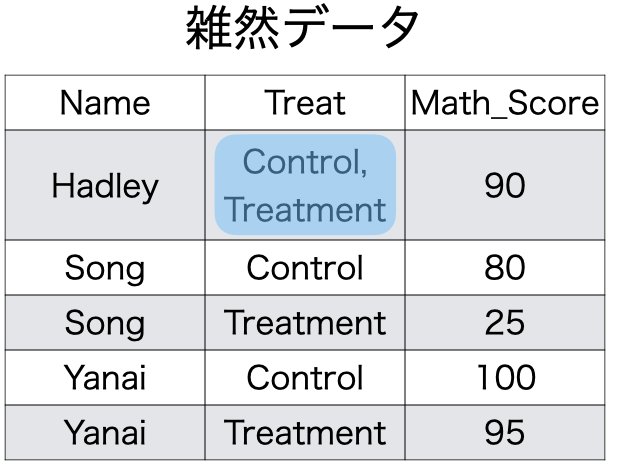
\includegraphics[width=0.5\textwidth,height=\textheight]{./Figs/Tidydata/TidyData3.png}

}

\caption{\label{fig-tidydata_example3}1つのセルは、1つの値を表す}

\end{figure}

図~\ref{fig-tidydata_example3}
の例は「1セル1値」の条件に明らかに反します。しかし、基準が曖昧な変数もあり、その一つが日付です。

\begin{table}

\caption{\label{tbl-tidydata_date_table}日付の扱い方}\begin{minipage}[t]{0.50\linewidth}
\subcaption{\label{tbl-tidydata_date_table-1}雑然データ? }

{\centering 

\raisebox{-\height}{

\centering
\begin{tabular}{lr}
\toprule
Date & Stock\\
\midrule
2020/06/29 & 100\\
2020/06/30 & 105\\
2020/07/01 & 110\\
2020/07/02 & 85\\
2020/07/03 & 90\\
\bottomrule
\end{tabular}

}

}

\end{minipage}%
%
\begin{minipage}[t]{0.50\linewidth}
\subcaption{\label{tbl-tidydata_date_table-2}整然データ? }

{\centering 

\raisebox{-\height}{

\centering
\begin{tabular}{rrrr}
\toprule
Year & Month & Date & Stock\\
\midrule
2020 & 6 & 29 & 100\\
2020 & 6 & 30 & 105\\
2020 & 7 & 1 & 110\\
2020 & 7 & 2 & 85\\
2020 & 7 & 3 & 90\\
\bottomrule
\end{tabular}

}

}

\end{minipage}%

\end{table}

表~\ref{tbl-tidydata_date_table}
の左側の表はどうでしょうか。5日間の株価を記録した架空のデータですが、たしかに\texttt{Date}列には日付が1つずつ、\texttt{Stock}には株価の値が1つずつ格納されています。しかし、解釈によっては「\texttt{Date}に年、月、日といった3つの値が含まれているぞ」と見ることもできます。この解釈に基づく場合、
表~\ref{tbl-tidydata_date_table}
の右側の表が整然データとなり、左側は雑然データとなります。このケースは第一条件であった「一列一変数」とも関係します。なぜなら、\texttt{Date}という列が年・月・日といった3変数で構成されているとも解釈できるからです。

分析によっては左側のような表でも全く問題ないケースもあります。時系列分析でトレンド変数のみ必要ならこれでも十分に整然データと呼べます。しかし、季節変動などの要素も考慮するならば、左側は雑然データになります。データとしての使い勝手は右側の方が優れているのは確かです。

データを出来る限り細かく分解するほど情報量が豊かになりますが、それにも限度はあるでしょう。たとえば、「\texttt{Year}は実は世紀の情報も含まれているのでは\ldots?」という解釈もできますが、これを反映してデータ整形を行うか否かは分析の目的と分析モデルによって異なります。この意味で、明らかな雑然データはあり得ますが、明らかな整然データは存在しないでしょう。どちらかといえば、整然さの度合いがあり、「これなら十分に整然データと言えないだろうか」と判断できれば十分ではないかと筆者
(Song)は考えます。

\hypertarget{ux3064ux306eux8868ux306f1ux3064ux306eux89b3ux6e2cux5358ux4f4dux3092ux3082ux3064}{%
\subsection{1つの表は、1つの観測単位をもつ}\label{ux3064ux306eux8868ux306f1ux3064ux306eux89b3ux6e2cux5358ux4f4dux3092ux3082ux3064}}

\href{https://www.e-stat.go.jp}{e-stat}などから\href{https://www.e-stat.go.jp/stat-search/database?page=1\&toukei=00200521\&tstat=000001080615}{国勢調査データ}をダウンロードした経験はあるでしょうか。以下の
図~\ref{fig-tidydata_example4} は2015年度国勢調査データの一部です。

\begin{figure}

{\centering 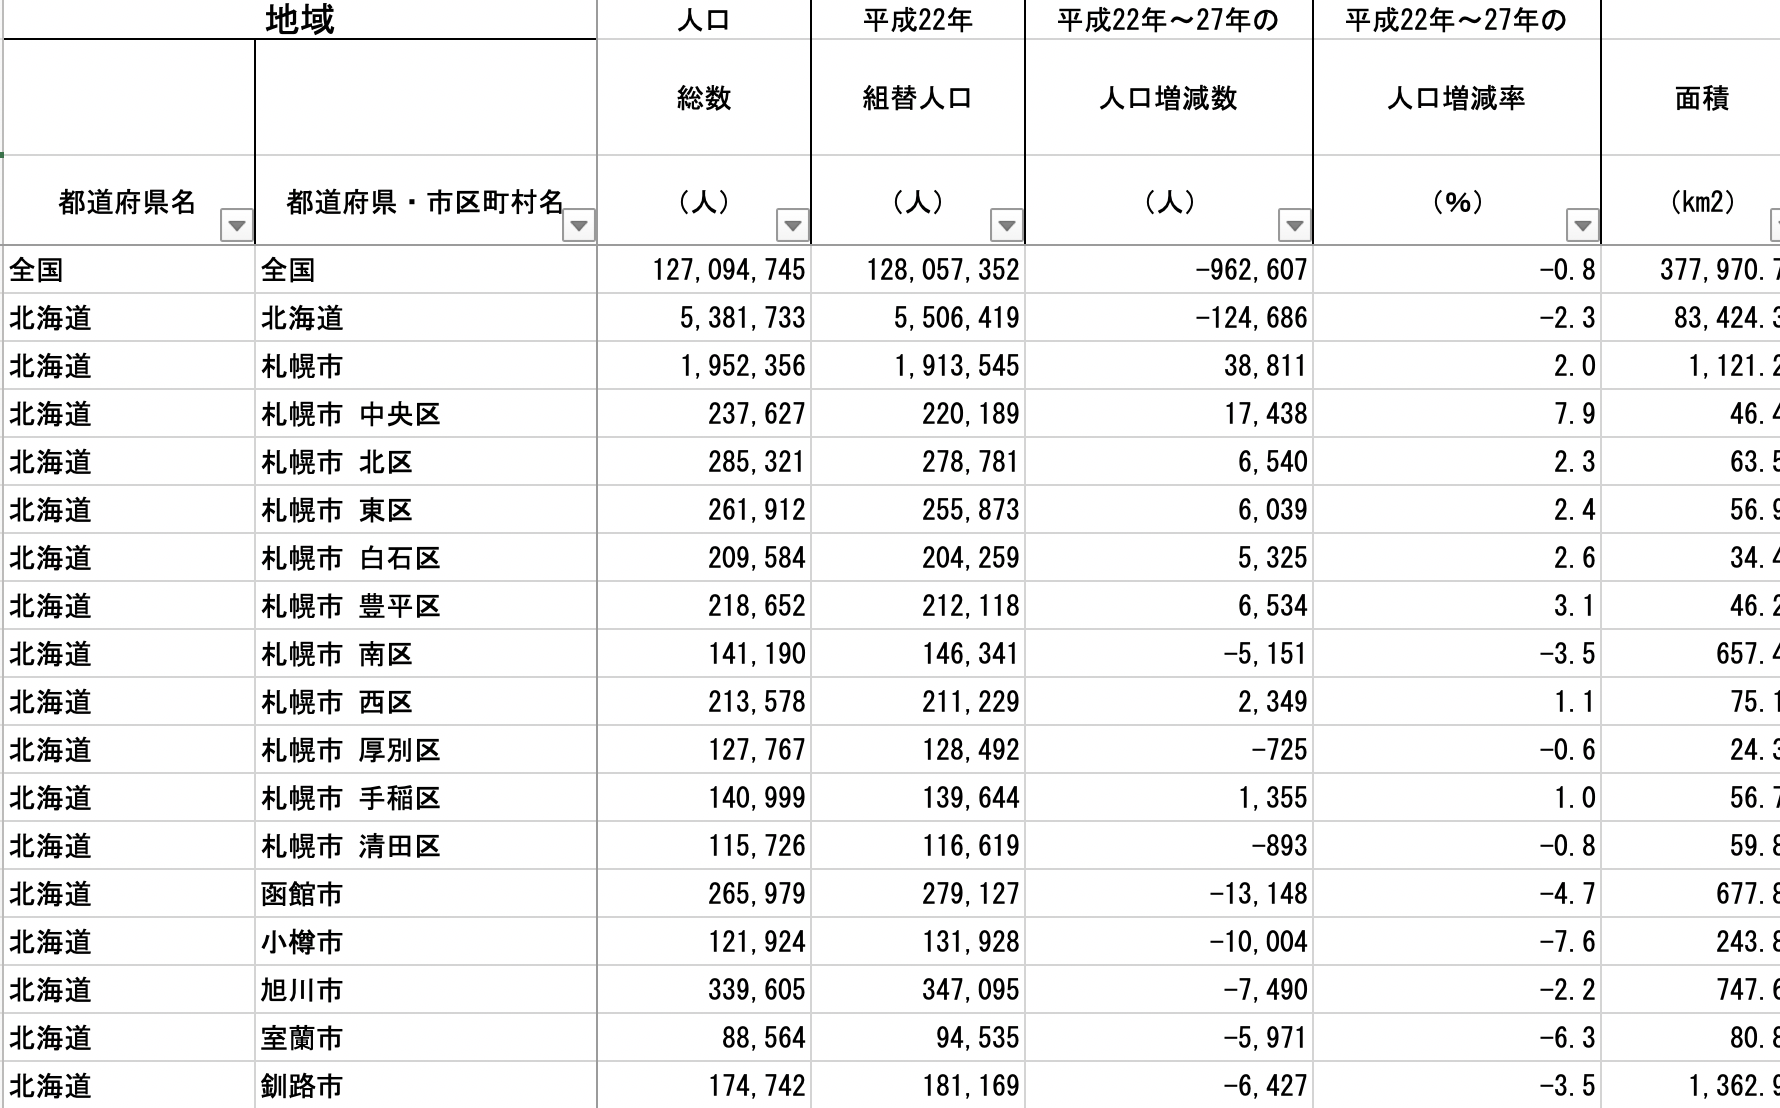
\includegraphics[width=0.5\textwidth,height=\textheight]{./Figs/Tidydata/MessyData4.png}

}

\caption{\label{fig-tidydata_example4}国勢調査データ}

\end{figure}

このデータの観察単位はなんでしょうか。データのの1行目は全国の人口を表しています。つまり、単位は国となります。しかし、2行目は北海道の人口です。この場合の観測単位は都道府県となります。つづいて、3行目は札幌市なので単位は市区町村になります。4行目は札幌市中央区、つまり観測単位が行政区になっています。そして14行目は函館市でまた単位は市区町村に戻っています。実際、会社や政府が作成するデータには
図~\ref{fig-tidydata_example4} や 図~\ref{fig-tidydata_example5}
のようなものが多いです。とりわけ、 図~\ref{fig-tidydata_example5}
のように、最後の行に「合計」などが表記されている場合が多いです。

\begin{figure}

{\centering \includegraphics[width=0.5\textwidth,height=\textheight]{./Figs/Tidydata/TidyData4.png}

}

\caption{\label{fig-tidydata_example5}1つの表は、1つの観測単位をもつ}

\end{figure}

このような表・データを作成することが悪いことではありません。むしろ、「読む」ための表ならこのような書き方が一般的でしょう。しかし、「分析」のためのデータは観察の単位を統一する必要があります。

\begin{center}\rule{0.5\linewidth}{0.5pt}\end{center}

\hypertarget{sec-tidydata_gather}{%
\section{Wide型からLong型へ}\label{sec-tidydata_gather}}

以下では「1列1変数」の条件を満たすデータの作成に便利な\texttt{pivot\_longer()}と\texttt{pivot\_wider()}関数について解説します。この関数群はおなじみの\{dplyr\}でなく、\{tidyr\}パッケージが提供している関数ですが、どれも\{tidyverse\}パッケージ群に含まれているため、\{tidyverse\}パッケージを読み込むだけで十分です。本節では\texttt{pivot\_longer()}を、次節では\texttt{pivot\_wider()}を取り上げます。

まず、\texttt{pivot\_longer()}ですが、この関数は比較的に新しい関数であり、これまでは\{tidyr\}の\texttt{gather()}関数が使われてきました。しかし、\texttt{gahter()}関数は将来、なくなる予定の関数であり、今から\{tidyr\}を学習する方は\texttt{pivot\_*()}関数群に慣れておきましょう。

まずは\texttt{tidyverse}パッケージを読み込みます。

\begin{Shaded}
\begin{Highlighting}[numbers=left,,]
\NormalTok{pacman}\SpecialCharTok{::}\FunctionTok{p\_load}\NormalTok{(tidyverse)}
\end{Highlighting}
\end{Shaded}

今回は様々な形のデータを変形する作業をするので、あるデータセットを使うよりも、架空の簡単なデータを使います。

\begin{Shaded}
\begin{Highlighting}[numbers=left,,]
\NormalTok{df1 }\OtherTok{\textless{}{-}} \FunctionTok{tibble}\NormalTok{(}
  \AttributeTok{Name      =} \FunctionTok{c}\NormalTok{(}\StringTok{"Hadley"}\NormalTok{, }\StringTok{"Song"}\NormalTok{, }\StringTok{"Yanai"}\NormalTok{),}
  \AttributeTok{Control   =} \FunctionTok{c}\NormalTok{(}\DecValTok{90}\NormalTok{, }\DecValTok{80}\NormalTok{, }\DecValTok{100}\NormalTok{),}
  \AttributeTok{Treatment =} \FunctionTok{c}\NormalTok{(}\DecValTok{90}\NormalTok{, }\DecValTok{25}\NormalTok{, }\DecValTok{95}\NormalTok{),}
  \AttributeTok{Gender    =} \FunctionTok{c}\NormalTok{(}\StringTok{"Male"}\NormalTok{, }\StringTok{"Female"}\NormalTok{, }\StringTok{"Female"}\NormalTok{)}
\NormalTok{)}

\NormalTok{df1}
\end{Highlighting}
\end{Shaded}

\begin{verbatim}
# A tibble: 3 x 4
  Name   Control Treatment Gender
  <chr>    <dbl>     <dbl> <chr> 
1 Hadley      90        90 Male  
2 Song        80        25 Female
3 Yanai      100        95 Female
\end{verbatim}

このデータは既に指摘した通り「1列1変数」の条件を満たしております。この条件を満たすデータは以下のような形となります。

\begin{verbatim}
# A tibble: 6 x 4
  Name   Gender Treat     Math_Score
  <chr>  <chr>  <chr>          <dbl>
1 Hadley Male   Control           90
2 Hadley Male   Treatment         90
3 Song   Female Control           80
4 Song   Female Treatment         25
5 Yanai  Female Control          100
6 Yanai  Female Treatment         95
\end{verbatim}

\texttt{Treat}変数が作成され、元々は変数名であった\texttt{"Control"}と\texttt{"Treatment"}が値として格納されます。この変数をキー変数と呼びます。そして、キー変数の値に応じた数学成績が\texttt{Math\_Score}という変数でまとめられました。この変数を値変数と呼びます。

「1列1変数」を満たさなかった最初のデータは「Wide型データ」、これを満たすようなデータは「Long型データ」と呼ばれます。これは相対的に最初のデータが横に広いから名付けた名前であって、「Wide型=雑然データ」もしくは「Long型=雑然データ」ではないことに注意してください\footnote{たとえば、
  表~\ref{tbl-tidydata_blood}
  は右の方がLong型データですが、整然データはWide型である左の方ですね。}。

Wide型データをLong型へ変換する関数が\texttt{pivot\_longer()}であり、基本的な使い方は以下の通りです。

\begin{Shaded}
\begin{Highlighting}[numbers=left,,]
\CommentTok{\# pivot\_longer()の使い方}
\NormalTok{データ名 }\SpecialCharTok{\%\textgreater{}\%}
  \FunctionTok{pivot\_longer}\NormalTok{(}\AttributeTok{cols      =} \FunctionTok{c}\NormalTok{(まとめる変数1, まとめる変数2, ...),}
               \AttributeTok{names\_to  =} \StringTok{"キー変数名"}\NormalTok{,}
               \AttributeTok{values\_to =} \StringTok{"値変数名"}\NormalTok{)}
\end{Highlighting}
\end{Shaded}

ここでは同じ変数が\texttt{Control}と\texttt{Treatment}変数で分けられているため、まとめる変数はこの2つであり、\texttt{cols\ =\ c(Control,\ Treatment)}と指定します。\texttt{Control}と\texttt{Treatment}は\texttt{"}で囲んでも、囲まなくても同じです。また、\texttt{dplyr}の\texttt{select()}関数で使える変数選択の関数
(\texttt{starts\_with()}、\texttt{where()}など)や\texttt{:}演算子も使用可能です。また、\texttt{cols}引数は\texttt{pivot\_longer()}の第2引数であるため、\texttt{cols\ =}は省略可能です(第一引数はパイプにより既に渡されています)。

\texttt{names\_to}と\texttt{values\_to}引数はそれぞれキー変数名と値変数名を指定する引数で、ここは必ず\texttt{"}で囲んでください。この\texttt{df1}をLong型へ変換し、\texttt{df1\_L}と名付けるコードが以下のコードです。

\begin{Shaded}
\begin{Highlighting}[numbers=left,,]
\NormalTok{df1\_L }\OtherTok{\textless{}{-}}\NormalTok{ df1 }\SpecialCharTok{\%\textgreater{}\%}
  \FunctionTok{pivot\_longer}\NormalTok{(Control}\SpecialCharTok{:}\NormalTok{Treatment,}
               \AttributeTok{names\_to  =} \StringTok{"Treat"}\NormalTok{,}
               \AttributeTok{values\_to =} \StringTok{"Math\_Score"}\NormalTok{)}

\NormalTok{df1\_L}
\end{Highlighting}
\end{Shaded}

\begin{verbatim}
# A tibble: 6 x 4
  Name   Gender Treat     Math_Score
  <chr>  <chr>  <chr>          <dbl>
1 Hadley Male   Control           90
2 Hadley Male   Treatment         90
3 Song   Female Control           80
4 Song   Female Treatment         25
5 Yanai  Female Control          100
6 Yanai  Female Treatment         95
\end{verbatim}

これだけでも\texttt{pivot\_longer()}関数を使ってWide型からLong型への変換は問題なくできますが、以下ではもうちょっと踏み込んだ使い方について解説します。「ここまでで十分だよ」という方は、ここを飛ばしても構いません。

今回の実習データ\texttt{df3}は3人の体重を3日間に渡って計測したものです。ただし、ドジっ子のSongは2日目にうっかり測るのを忘れており、欠損値となっています。

\begin{Shaded}
\begin{Highlighting}[numbers=left,,]
\NormalTok{df2 }\OtherTok{\textless{}{-}} \FunctionTok{tibble}\NormalTok{(}
  \AttributeTok{Name =} \FunctionTok{c}\NormalTok{(}\StringTok{"Hadley"}\NormalTok{, }\StringTok{"Song"}\NormalTok{, }\StringTok{"Yanai"}\NormalTok{),}
  \AttributeTok{Day1 =} \FunctionTok{c}\NormalTok{(}\DecValTok{75}\NormalTok{, }\DecValTok{120}\NormalTok{, }\DecValTok{70}\NormalTok{),}
  \AttributeTok{Day2 =} \FunctionTok{c}\NormalTok{(}\DecValTok{73}\NormalTok{,  }\ConstantTok{NA}\NormalTok{, }\DecValTok{69}\NormalTok{),}
  \AttributeTok{Day3 =} \FunctionTok{c}\NormalTok{(}\DecValTok{71}\NormalTok{, }\DecValTok{140}\NormalTok{, }\DecValTok{71}\NormalTok{)}
\NormalTok{)}

\NormalTok{df2}
\end{Highlighting}
\end{Shaded}

\begin{verbatim}
# A tibble: 3 x 4
  Name    Day1  Day2  Day3
  <chr>  <dbl> <dbl> <dbl>
1 Hadley    75    73    71
2 Song     120    NA   140
3 Yanai     70    69    71
\end{verbatim}

まず、これをこれまでのやり方でLong型へ変形し、\texttt{df2\_L}と名付けます。

\begin{Shaded}
\begin{Highlighting}[numbers=left,,]
\NormalTok{df2\_L }\OtherTok{\textless{}{-}}\NormalTok{ df2 }\SpecialCharTok{\%\textgreater{}\%}
  \FunctionTok{pivot\_longer}\NormalTok{(}\FunctionTok{starts\_with}\NormalTok{(}\StringTok{"Day"}\NormalTok{),}
               \AttributeTok{names\_to  =} \StringTok{"Days"}\NormalTok{,}
               \AttributeTok{values\_to =} \StringTok{"Weight"}\NormalTok{)}

\NormalTok{df2\_L}
\end{Highlighting}
\end{Shaded}

\begin{verbatim}
# A tibble: 9 x 3
  Name   Days  Weight
  <chr>  <chr>  <dbl>
1 Hadley Day1      75
2 Hadley Day2      73
3 Hadley Day3      71
4 Song   Day1     120
5 Song   Day2      NA
6 Song   Day3     140
7 Yanai  Day1      70
8 Yanai  Day2      69
9 Yanai  Day3      71
\end{verbatim}

これでも問題ないかも知れませんが、以下のような操作を追加に行うとします。

\begin{enumerate}
\def\labelenumi{\arabic{enumi}.}
\tightlist
\item
  \texttt{Weight}が欠損している行を除去する
\item
  \texttt{Days}列の値から\texttt{"Day"}を除去し、numeric型にする
\end{enumerate}

以上の作業を行うには、\texttt{dplyr}が便利でしょう。ちなみに\texttt{str\_remove()}関数が初めて登場しましたが、これについては第\ref{sec-string}章で詳細に解説します。簡単に説明しますと、\texttt{str\_remove("X123",\ "X")}は\texttt{"X123"}から\texttt{"X"}を除去し、\texttt{"123"}のみ残す関すです。残された値が数字のみであってもデータ型はcharacter型なので、もう一回、numeric型に変換する必要があります\footnote{実は\texttt{parse\_number()}を使えばもっと簡単ですが、これについては後ほど解説します。}。\texttt{dplyr}を使ったコードは以下の通りです。

\begin{Shaded}
\begin{Highlighting}[numbers=left,,]
\CommentTok{\# 1. WeightがNAのケースを除去}
\CommentTok{\# 2. Days変数の値から"Day"を除去}
\CommentTok{\# 3. Days変数をnumeric型へ変換}
\NormalTok{df2\_L }\SpecialCharTok{\%\textgreater{}\%}
  \FunctionTok{filter}\NormalTok{(}\SpecialCharTok{!}\FunctionTok{is.na}\NormalTok{(Weight)) }\SpecialCharTok{\%\textgreater{}\%}           \CommentTok{\# 1}
  \FunctionTok{mutate}\NormalTok{(}\AttributeTok{Days =} \FunctionTok{str\_remove}\NormalTok{(Days, }\StringTok{"Day"}\NormalTok{), }\CommentTok{\# 2}
         \AttributeTok{Days =} \FunctionTok{as.numeric}\NormalTok{(Days))        }\CommentTok{\# 3}
\end{Highlighting}
\end{Shaded}

\begin{verbatim}
# A tibble: 8 x 3
  Name    Days Weight
  <chr>  <dbl>  <dbl>
1 Hadley     1     75
2 Hadley     2     73
3 Hadley     3     71
4 Song       1    120
5 Song       3    140
6 Yanai      1     70
7 Yanai      2     69
8 Yanai      3     71
\end{verbatim}

実はこの作業、\texttt{pivot\_longer()}内で行うことも可能です。たとえば、\texttt{values\_to}で指定した変数の値が欠損しているケースを除去するには\texttt{values\_drop\_na}引数を\texttt{TRUE}に指定するだけです。

\begin{Shaded}
\begin{Highlighting}[numbers=left,,]
\CommentTok{\# Weight変数がNAのケースを除去する}
\NormalTok{df2 }\SpecialCharTok{\%\textgreater{}\%}
  \FunctionTok{pivot\_longer}\NormalTok{(}\FunctionTok{starts\_with}\NormalTok{(}\StringTok{"Day"}\NormalTok{),}
               \AttributeTok{names\_to       =} \StringTok{"Days"}\NormalTok{,}
               \AttributeTok{values\_to      =} \StringTok{"Weight"}\NormalTok{,}
               \AttributeTok{values\_drop\_na =} \ConstantTok{TRUE}\NormalTok{)}
\end{Highlighting}
\end{Shaded}

\begin{verbatim}
# A tibble: 8 x 3
  Name   Days  Weight
  <chr>  <chr>  <dbl>
1 Hadley Day1      75
2 Hadley Day2      73
3 Hadley Day3      71
4 Song   Day1     120
5 Song   Day3     140
6 Yanai  Day1      70
7 Yanai  Day2      69
8 Yanai  Day3      71
\end{verbatim}

それでは、キー変数から共通する文字列を除去するにはどうすれば良いでしょうか。この場合、\texttt{names\_prefix}引数を使います。これは\texttt{names\_to}で指定した新しく出来る変数の値における接頭詞を指定し、それを除去する引数です。今回は\texttt{"Day1"}、\texttt{"Day2"}、\texttt{"Day3"}から\texttt{"Day"}を除去するので、\texttt{names\_prefix\ =\ "Day"}と指定します。こうすることで、\texttt{Days}列から\texttt{"Day"}が除去されます。ただし、数字だけ残っても、そのデータ型はcharacter型ですので、このデータ型を変換する必要があります。ここで使うのが\texttt{names\_transform}引数であり、これはlist型のオブジェクトを渡す必要があります。\texttt{Days}列をnumeric型にする場合は\texttt{list(Days\ =\ as.numeric)}です。複数の列のデータ型を変える場合、\texttt{list()}の中に追加していきます。それでは実際に走らせてみましょう。

\begin{Shaded}
\begin{Highlighting}[numbers=left,,]
\CommentTok{\# 1. Day変数の値から"Day"を除去する}
\CommentTok{\# 2. Day変数をinteger型に変換}
\CommentTok{\# 3. Weight変数がNAのケースを除去する}
\NormalTok{df2 }\SpecialCharTok{\%\textgreater{}\%}
  \FunctionTok{pivot\_longer}\NormalTok{(}\FunctionTok{starts\_with}\NormalTok{(}\StringTok{"Day"}\NormalTok{),}
               \AttributeTok{names\_to        =} \StringTok{"Days"}\NormalTok{,}
               \AttributeTok{names\_prefix    =} \StringTok{"Day"}\NormalTok{,                   }\CommentTok{\# 1}
               \AttributeTok{names\_transform =} \FunctionTok{list}\NormalTok{(}\AttributeTok{Days =}\NormalTok{ as.numeric), }\CommentTok{\# 2}
               \AttributeTok{values\_to       =} \StringTok{"Weight"}\NormalTok{,}
               \AttributeTok{values\_drop\_na  =} \ConstantTok{TRUE}\NormalTok{)                    }\CommentTok{\# 3}
\end{Highlighting}
\end{Shaded}

\begin{verbatim}
# A tibble: 8 x 3
  Name    Days Weight
  <chr>  <dbl>  <dbl>
1 Hadley     1     75
2 Hadley     2     73
3 Hadley     3     71
4 Song       1    120
5 Song       3    140
6 Yanai      1     70
7 Yanai      2     69
8 Yanai      3     71
\end{verbatim}

これでWide型をLong型が変換され、整然でありながら、より見栄の良いデータが出来上がりました。他にも\texttt{pivot\_longer()}は様々な引数に対応しており、詳細は\texttt{?pivot\_longer}や\href{https://tidyr.tidyverse.org/reference/pivot_longer.html}{レファレンスページ}を参照してください。

\begin{center}\rule{0.5\linewidth}{0.5pt}\end{center}

\hypertarget{sec-tidydata_spread}{%
\section{Long型からWide型へ}\label{sec-tidydata_spread}}

ご存知の通り、「Long型データ=整然データ」ではありません。実際、
表~\ref{tbl-tidydata_blood}
の右はLong型データですが、1列に2つの変数が含まれており、整然データとは言えません。このようなデータはいくらでもあります。とりわけ、「分析」のためじゃなく、「読む」ための表の場合において多く発見されます。

\begin{table}

\caption{\label{tbl-tidydata_wider1}Long型データの例}\begin{minipage}[t]{0.50\linewidth}
\subcaption{\label{tbl-tidydata_wider1-1}雑然データ }

{\centering 

\raisebox{-\height}{

\centering
\begin{tabular}{llrr}
\toprule
都道府県 & 区分 & 人口 & 面積\\
\midrule
北海道 & 総人口 & 5381733 & 83424.31\\
 & 外国人 & 21676 & 83424.31\\
青森県 & 総人口 & 1308265 & 9645.59\\
 & 外国人 & 3447 & 9645.59\\
岩手県 & 総人口 & 1279594 & 15275.01\\
\addlinespace
 & 外国人 & 5017 & 15275.01\\
宮城県 & 総人口 & 2333899 & 7282.22\\
 & 外国人 & 13989 & 7282.22\\
\bottomrule
\end{tabular}

}

}

\end{minipage}%
%
\begin{minipage}[t]{0.50\linewidth}
\subcaption{\label{tbl-tidydata_wider1-2}整然データ }

{\centering 

\raisebox{-\height}{

\centering
\begin{tabular}{lrrr}
\toprule
都道府県 & 総人口 & 外国人 & 面積\\
\midrule
北海道 & 5381733 & 21676 & 83424.31\\
青森県 & 1308265 & 3447 & 9645.59\\
岩手県 & 1279594 & 5017 & 15275.01\\
宮城県 & 2333899 & 13989 & 7282.22\\
\bottomrule
\end{tabular}

}

}

\end{minipage}%

\end{table}

変数名が日本語になっていますが、これは「読むための表」を読み込むことを仮定しています。このように変数名として日本語は使えますが、自分でデータセットを作成する際、変数名はローマ字にすることを強く推奨します。

表~\ref{tbl-tidydata_wider1}
の左の場合、\texttt{人口}列に総人口と外国人人口といった2つの変数の値が格納されているため、整然データではありません。これを整然データにしたものが右の表です。本節ではLong型データをWide型データへ変換する\texttt{pivot\_wider()}関数を紹介します。この関数は同じく\texttt{tidyr}が提供している\texttt{spread()}関数とほぼ同じ関数ですが、今は\texttt{pivot\_wider()}の使用が推奨されており、\texttt{spread()}はいずれか\texttt{tidyr}から外される予定です。

まずは、実習用データを読み込みます。

\begin{Shaded}
\begin{Highlighting}[numbers=left,,]
\NormalTok{df3 }\OtherTok{\textless{}{-}} \FunctionTok{read\_csv}\NormalTok{(}\StringTok{"Data/Population2015.csv"}\NormalTok{)}

\NormalTok{df3}
\end{Highlighting}
\end{Shaded}

\begin{verbatim}
# A tibble: 94 x 4
   都道府県 区分      人口   面積
   <chr>    <chr>    <dbl>  <dbl>
 1 北海道   総人口 5381733 83424.
 2 <NA>     外国人   21676 83424.
 3 青森県   総人口 1308265  9646.
 4 <NA>     外国人    3447  9646.
 5 岩手県   総人口 1279594 15275.
 6 <NA>     外国人    5017 15275.
 7 宮城県   総人口 2333899  7282.
 8 <NA>     外国人   13989  7282.
 9 秋田県   総人口 1023119 11638.
10 <NA>     外国人    2914 11638.
# ... with 84 more rows
\end{verbatim}

このデータは2015年国勢調査から抜粋したデータであり、各変数の詳細は
表~\ref{tbl-tidydata_df3_detail} の通りです。

\hypertarget{tbl-tidydata_df3_detail}{}
\begin{table}
\caption{\label{tbl-tidydata_df3_detail}df3の詳細 }

\centering
\begin{tabular}{l|l}
\hline
\multicolumn{1}{c}{変数名} & \multicolumn{1}{c}{説明}\\
\hline
`都道府県` & 都道府県名\\
\hline
`区分` & 総人口/外国人人口の区分\\
\hline
`人口` & 人口 (人)\\
\hline
`面積` & 面積 (km\$\textasciicircum{}2\$)\\
\hline
\end{tabular}
\end{table}

まずは変数名が日本語になっているので、\texttt{rename()}関数を使ってそれぞれ\texttt{Pref}、\texttt{Type}、\texttt{Population}、\texttt{Area}に変更します。

\begin{Shaded}
\begin{Highlighting}[numbers=left,,]
\NormalTok{df3 }\OtherTok{\textless{}{-}}\NormalTok{ df3 }\SpecialCharTok{\%\textgreater{}\%}
  \FunctionTok{rename}\NormalTok{(}\StringTok{"Pref"} \OtherTok{=}\NormalTok{ 都道府県, }\StringTok{"Type"} \OtherTok{=}\NormalTok{ 区分, }\StringTok{"Population"} \OtherTok{=}\NormalTok{ 人口, }\StringTok{"Area"} \OtherTok{=}\NormalTok{ 面積)}

\NormalTok{df3}
\end{Highlighting}
\end{Shaded}

\begin{verbatim}
# A tibble: 94 x 4
   Pref   Type   Population   Area
   <chr>  <chr>       <dbl>  <dbl>
 1 北海道 総人口    5381733 83424.
 2 <NA>   外国人      21676 83424.
 3 青森県 総人口    1308265  9646.
 4 <NA>   外国人       3447  9646.
 5 岩手県 総人口    1279594 15275.
 6 <NA>   外国人       5017 15275.
 7 宮城県 総人口    2333899  7282.
 8 <NA>   外国人      13989  7282.
 9 秋田県 総人口    1023119 11638.
10 <NA>   外国人       2914 11638.
# ... with 84 more rows
\end{verbatim}

次は、\texttt{Pref}列の欠損値を埋めましょう。ここの欠損値は、当該セルの一つ上のセルの値で埋まりますが、これは\texttt{fill()}関数で簡単に処理できます。欠損値を埋めたい変数名を\texttt{fill()}の引数として渡すだけです。

\begin{Shaded}
\begin{Highlighting}[numbers=left,,]
\NormalTok{df3 }\OtherTok{\textless{}{-}}\NormalTok{ df3 }\SpecialCharTok{\%\textgreater{}\%}
  \FunctionTok{fill}\NormalTok{(Pref)}

\NormalTok{df3}
\end{Highlighting}
\end{Shaded}

\begin{verbatim}
# A tibble: 94 x 4
   Pref   Type   Population   Area
   <chr>  <chr>       <dbl>  <dbl>
 1 北海道 総人口    5381733 83424.
 2 北海道 外国人      21676 83424.
 3 青森県 総人口    1308265  9646.
 4 青森県 外国人       3447  9646.
 5 岩手県 総人口    1279594 15275.
 6 岩手県 外国人       5017 15275.
 7 宮城県 総人口    2333899  7282.
 8 宮城県 外国人      13989  7282.
 9 秋田県 総人口    1023119 11638.
10 秋田県 外国人       2914 11638.
# ... with 84 more rows
\end{verbatim}

そして、いよいよ\texttt{pivot\_wider()}関数の出番ですが、基本的に使い方は以下の通りです。

\begin{Shaded}
\begin{Highlighting}[numbers=left,,]
\CommentTok{\# pivot\_wider()の使い方}
\NormalTok{データ名 }\SpecialCharTok{\%\textgreater{}\%}
  \FunctionTok{pivot\_wider}\NormalTok{(}\AttributeTok{names\_from  =}\NormalTok{ キー変数名,}
              \AttributeTok{values\_from =}\NormalTok{ 値変数名)}
\end{Highlighting}
\end{Shaded}

まず、キー変数名は列として展開する変数名であり、ここでは\texttt{Type}になります。そして、値変数名は展開される値の変数であり、ここでは\texttt{Population}になります。つまり、「\texttt{Population}を\texttt{Type}ごとに分けて別の列にする」ことになります。また、\texttt{values\_from}引数は長さ2以上のベクトルを指定することで、複数の値変数を指定することも可能です。たとえば、\texttt{df3}に\texttt{Income}という平均所得を表す列があり、これらも総人口と外国人それぞれ異なる値を持っているとしたら、\texttt{values\_from\ =\ c(Population,\ Income)}のように複数の値変数を指定することが出来ます。今回は値変数が1つのみですが、早速やってみましょう。

\begin{Shaded}
\begin{Highlighting}[numbers=left,,]
\NormalTok{df3\_W }\OtherTok{\textless{}{-}}\NormalTok{ df3 }\SpecialCharTok{\%\textgreater{}\%}
  \FunctionTok{pivot\_wider}\NormalTok{(}\AttributeTok{names\_from  =}\NormalTok{ Type,}
              \AttributeTok{values\_from =}\NormalTok{ Population)}

\NormalTok{df3\_W}
\end{Highlighting}
\end{Shaded}

\begin{verbatim}
# A tibble: 47 x 4
   Pref     Area  総人口 外国人
   <chr>   <dbl>   <dbl>  <dbl>
 1 北海道 83424. 5381733  21676
 2 青森県  9646. 1308265   3447
 3 岩手県 15275. 1279594   5017
 4 宮城県  7282. 2333899  13989
 5 秋田県 11638. 1023119   2914
 6 山形県  9323. 1123891   5503
 7 福島県 13784. 1914039   8725
 8 茨城県  6097. 2916976  41310
 9 栃木県  6408. 1974255  26494
10 群馬県  6362. 1973115  37126
# ... with 37 more rows
\end{verbatim}

また、日本語の変数名が出来てしまったので、それぞれ\texttt{Total}と\texttt{Foreigner}に変更し、\texttt{relocate()}関数を使って\texttt{Area}を最後の列に移動します。

\begin{Shaded}
\begin{Highlighting}[numbers=left,,]
\NormalTok{df3\_W }\OtherTok{\textless{}{-}}\NormalTok{ df3\_W }\SpecialCharTok{\%\textgreater{}\%}
  \FunctionTok{rename}\NormalTok{(}\StringTok{"Total"}     \OtherTok{=}\NormalTok{ 総人口,}
         \StringTok{"Foreigner"} \OtherTok{=}\NormalTok{ 外国人) }\SpecialCharTok{\%\textgreater{}\%}
  \FunctionTok{relocate}\NormalTok{(Area, }\AttributeTok{.after =} \FunctionTok{last\_col}\NormalTok{())}

\NormalTok{df3\_W}
\end{Highlighting}
\end{Shaded}

\begin{verbatim}
# A tibble: 47 x 4
   Pref     Total Foreigner   Area
   <chr>    <dbl>     <dbl>  <dbl>
 1 北海道 5381733     21676 83424.
 2 青森県 1308265      3447  9646.
 3 岩手県 1279594      5017 15275.
 4 宮城県 2333899     13989  7282.
 5 秋田県 1023119      2914 11638.
 6 山形県 1123891      5503  9323.
 7 福島県 1914039      8725 13784.
 8 茨城県 2916976     41310  6097.
 9 栃木県 1974255     26494  6408.
10 群馬県 1973115     37126  6362.
# ... with 37 more rows
\end{verbatim}

これで整然データの出来上がりです。

この\texttt{pivot\_wider()}関数は\texttt{pivot\_longer()}関数同様、様々な引数を提供しておりますが、主に使う機能は以上です。他には\texttt{pivot\_wider()}によって出来た欠損値を埋める引数である\texttt{values\_fill}があり、デフォルト値は\texttt{NULL}です。ここに\texttt{0}や\texttt{"Missing"}などの長さ1のベクトルを指定すれば、指定した値で欠損値が埋まります。

\texttt{pivot\_wider()}関数の詳細は\texttt{?pivot\_wider}もしくは、\href{https://tidyr.tidyverse.org/reference/pivot_wider.html}{レファレンスページ}を参照してください。

\begin{center}\rule{0.5\linewidth}{0.5pt}\end{center}

\hypertarget{sec-tidydata_separate}{%
\section{列の操作}\label{sec-tidydata_separate}}

他にも「1列1変数」の条件を満たさないケースを考えましょう。\texttt{pivot\_longer()}は1つの変数が複数の列に渡って格納されている際に使いましたが、今回は1つの列に複数の変数があるケースを考えてみましょう。たとえば、年月日が1つの列に入っている場合、これを年、月、日の3列で分割する作業です。また、これと関連して、列から文字列を除去し、数値のみ残す方法についても紹介します。

\href{Data/COVID19_JK.csv}{実習用データ}を読み込んでみましょう。

\begin{Shaded}
\begin{Highlighting}[numbers=left,,]
\NormalTok{df4 }\OtherTok{\textless{}{-}} \FunctionTok{read\_csv}\NormalTok{(}\StringTok{"Data/COVID19\_JK.csv"}\NormalTok{)}
\end{Highlighting}
\end{Shaded}

\begin{verbatim}
Rows: 172 Columns: 5
-- Column specification --------------------------------------------------------
Delimiter: ","
chr (4): Date, Week, Confirmed_Japan, Confirmed_Korea
dbl (1): ID

i Use `spec()` to retrieve the full column specification for this data.
i Specify the column types or set `show_col_types = FALSE` to quiet this message.
\end{verbatim}

\begin{Shaded}
\begin{Highlighting}[numbers=left,,]
\NormalTok{df4}
\end{Highlighting}
\end{Shaded}

\begin{verbatim}
# A tibble: 172 x 5
      ID Date      Week  Confirmed_Japan Confirmed_Korea
   <dbl> <chr>     <chr> <chr>           <chr>          
 1     1 2020/1/16 木    1人             <NA>           
 2     2 2020/1/17 金    0人             <NA>           
 3     3 2020/1/18 土    0人             <NA>           
 4     4 2020/1/19 日    0人             <NA>           
 5     5 2020/1/20 月    0人             1人            
 6     6 2020/1/21 火    0人             0人            
 7     7 2020/1/22 水    0人             0人            
 8     8 2020/1/23 木    0人             0人            
 9     9 2020/1/24 金    2人             1人            
10    10 2020/1/25 土    0人             0人            
# ... with 162 more rows
\end{verbatim}

このデータは2020年1月16日から2020年7月5日まで、COVID-19
(新型コロナ)の新規感染者数を日本と韓国を対象に収集したものです。データはWikipedia
(\href{https://en.wikipedia.org/wiki/COVID-19_pandemic_in_Japan}{日本} /
\href{https://en.wikipedia.org/wiki/COVID-19_pandemic_in_South_Korea}{韓国})から収集しました。韓国の新規感染者数は最初の4日分が欠損値のように見えますが、最初の感染者が確認されたのが1月20日のため、1月19日までは欠損となっています。

\begin{table}
\centering
\begin{tabular}{l|l}
\hline
\multicolumn{1}{c}{変数名} & \multicolumn{1}{c}{説明}\\
\hline
`ID` & ケースID\\
\hline
`Date` & 年月日\\
\hline
`Week` & 曜日\\
\hline
`Confirmed\_Japan` & 新規感染者数 (日本)\\
\hline
`Confirmed\_Korea` & 新規感染者数 (韓国)\\
\hline
\end{tabular}
\end{table}

このデータの場合、観察単位は「国 \(\times\)
日」です。しかし、\texttt{df4}は1行に日本と韓国の情報が格納されており「1行1観察」の条件を満たしておりません。したがって、\texttt{pivot\_longer()}を使ってLong型へ変換し、新しいデータの名前を\texttt{df4\_L}と名付けます。

\begin{Shaded}
\begin{Highlighting}[numbers=left,,]
\NormalTok{df4\_L }\OtherTok{\textless{}{-}}\NormalTok{ df4 }\SpecialCharTok{\%\textgreater{}\%}
  \FunctionTok{pivot\_longer}\NormalTok{(}\AttributeTok{cols         =} \FunctionTok{starts\_with}\NormalTok{(}\StringTok{"Confirmed"}\NormalTok{), }
               \AttributeTok{names\_to     =} \StringTok{"Country"}\NormalTok{,}
               \AttributeTok{names\_prefix =} \StringTok{"Confirmed\_"}\NormalTok{,}
               \AttributeTok{values\_to    =} \StringTok{"Confirmed"}\NormalTok{)}

\NormalTok{df4\_L}
\end{Highlighting}
\end{Shaded}

\begin{verbatim}
# A tibble: 344 x 5
      ID Date      Week  Country Confirmed
   <dbl> <chr>     <chr> <chr>   <chr>    
 1     1 2020/1/16 木    Japan   1人      
 2     1 2020/1/16 木    Korea   <NA>     
 3     2 2020/1/17 金    Japan   0人      
 4     2 2020/1/17 金    Korea   <NA>     
 5     3 2020/1/18 土    Japan   0人      
 6     3 2020/1/18 土    Korea   <NA>     
 7     4 2020/1/19 日    Japan   0人      
 8     4 2020/1/19 日    Korea   <NA>     
 9     5 2020/1/20 月    Japan   0人      
10     5 2020/1/20 月    Korea   1人      
# ... with 334 more rows
\end{verbatim}

続いて、新規感染者数を表す\texttt{Confirmed}列から「人」を除去しましょう。人間にとってはなんの問題もありませんが、パソコンにとって\texttt{1人}や\texttt{5人}は文字列に過ぎず、分析ができる状態ではありません。ここで使う関数が\texttt{parse\_number()}です。引数として指定した列から数値のみ抽出します。\texttt{"\$1000"}や\texttt{"1,\ 324,\ 392"}のような数値でありながら、character型として保存されている列から数値のみを取り出す際に使う関数です。使い方は以下の通りです。

\begin{Shaded}
\begin{Highlighting}[numbers=left,,]
\NormalTok{データ名 }\SpecialCharTok{\%\textgreater{}\%}
  \FunctionTok{mutate}\NormalTok{(新しい変数名 }\OtherTok{=} \FunctionTok{parse\_number}\NormalTok{(数値のみ抽出する変数名))}
\end{Highlighting}
\end{Shaded}

似たようなものとして\texttt{parse\_character()}があり、これは逆に文字列のみ抽出する関数です。

ここでは\texttt{Confimed}から数値のみ取り出し、\texttt{Confrimed}列に上書きし、それを\texttt{df4\_S}と名付けます。

\begin{Shaded}
\begin{Highlighting}[numbers=left,,]
\NormalTok{df4\_S }\OtherTok{\textless{}{-}}\NormalTok{ df4\_L }\SpecialCharTok{\%\textgreater{}\%}
  \FunctionTok{mutate}\NormalTok{(}\AttributeTok{Confirmed =} \FunctionTok{parse\_number}\NormalTok{(Confirmed))}

\NormalTok{df4\_S}
\end{Highlighting}
\end{Shaded}

\begin{verbatim}
# A tibble: 344 x 5
      ID Date      Week  Country Confirmed
   <dbl> <chr>     <chr> <chr>       <dbl>
 1     1 2020/1/16 木    Japan           1
 2     1 2020/1/16 木    Korea          NA
 3     2 2020/1/17 金    Japan           0
 4     2 2020/1/17 金    Korea          NA
 5     3 2020/1/18 土    Japan           0
 6     3 2020/1/18 土    Korea          NA
 7     4 2020/1/19 日    Japan           0
 8     4 2020/1/19 日    Korea          NA
 9     5 2020/1/20 月    Japan           0
10     5 2020/1/20 月    Korea           1
# ... with 334 more rows
\end{verbatim}

それでは国、曜日ごとの新規感染者数を調べてみます。求める統計量は曜日ごとの新規感染者数の合計、平均、標準偏差です。まず、曜日は月から日の順になるよう、factor型に変換します。そして、国と曜日ごとに記述統計量を計算し、\texttt{df4\_S\_Summary1}という名で保存します。

\begin{Shaded}
\begin{Highlighting}[numbers=left,,]
\NormalTok{df4\_S }\OtherTok{\textless{}{-}}\NormalTok{ df4\_S }\SpecialCharTok{\%\textgreater{}\%}
  \FunctionTok{mutate}\NormalTok{(}\AttributeTok{Week =} \FunctionTok{factor}\NormalTok{(Week, }
                       \AttributeTok{levels =} \FunctionTok{c}\NormalTok{(}\StringTok{"月"}\NormalTok{, }\StringTok{"火"}\NormalTok{, }\StringTok{"水"}\NormalTok{, }\StringTok{"木"}\NormalTok{, }\StringTok{"金"}\NormalTok{, }\StringTok{"土"}\NormalTok{, }\StringTok{"日"}\NormalTok{)))}

\NormalTok{df4\_S\_Summary1 }\OtherTok{\textless{}{-}}\NormalTok{ df4\_S }\SpecialCharTok{\%\textgreater{}\%}
  \FunctionTok{group\_by}\NormalTok{(Country, Week) }\SpecialCharTok{\%\textgreater{}\%}
  \FunctionTok{summarise}\NormalTok{(}\AttributeTok{Sum     =} \FunctionTok{sum}\NormalTok{(Confirmed,  }\AttributeTok{na.rm =} \ConstantTok{TRUE}\NormalTok{),}
            \AttributeTok{Mean    =} \FunctionTok{mean}\NormalTok{(Confirmed, }\AttributeTok{na.rm =} \ConstantTok{TRUE}\NormalTok{),}
            \AttributeTok{SD      =} \FunctionTok{sd}\NormalTok{(Confirmed,   }\AttributeTok{na.rm =} \ConstantTok{TRUE}\NormalTok{),}
            \AttributeTok{.groups =} \StringTok{"drop"}\NormalTok{)}

\NormalTok{df4\_S\_Summary1}
\end{Highlighting}
\end{Shaded}

\begin{verbatim}
# A tibble: 14 x 5
   Country Week    Sum  Mean    SD
   <chr>   <fct> <dbl> <dbl> <dbl>
 1 Japan   月     2540 106.   156.
 2 Japan   火     2093  87.2  111.
 3 Japan   水     2531 105.   133.
 4 Japan   木     2704 108.   151.
 5 Japan   金     3083 123.   172.
 6 Japan   土     3327 133.   189.
 7 Japan   日     3244 130.   179.
 8 Korea   月     1609  67.0  126.
 9 Korea   火     1641  68.4  111.
10 Korea   水     1626  67.8  102.
11 Korea   木     1883  78.5  137.
12 Korea   金     2099  87.5  143.
13 Korea   土     2194  91.4  174.
14 Korea   日     2088  87    215.
\end{verbatim}

\texttt{df4\_S\_Summary1}はこの状態で整然データですが、もし人間が読むための表を作るなら、韓国と日本を別の列に分けた方が良いかも知れません。\texttt{pivot\_wider()}を使って、日本と韓国のの新規感染者数を2列に展開します。

\begin{Shaded}
\begin{Highlighting}[numbers=left,,]
\NormalTok{df4\_S\_Summary1 }\SpecialCharTok{\%\textgreater{}\%}
  \FunctionTok{pivot\_wider}\NormalTok{(}\AttributeTok{names\_from  =}\NormalTok{ Country,}
              \AttributeTok{values\_from =}\NormalTok{ Sum}\SpecialCharTok{:}\NormalTok{SD)}
\end{Highlighting}
\end{Shaded}

\begin{verbatim}
# A tibble: 7 x 7
  Week  Sum_Japan Sum_Korea Mean_Japan Mean_Korea SD_Japan SD_Korea
  <fct>     <dbl>     <dbl>      <dbl>      <dbl>    <dbl>    <dbl>
1 月         2540      1609      106.        67.0     156.     126.
2 火         2093      1641       87.2       68.4     111.     111.
3 水         2531      1626      105.        67.8     133.     102.
4 木         2704      1883      108.        78.5     151.     137.
5 金         3083      2099      123.        87.5     172.     143.
6 土         3327      2194      133.        91.4     189.     174.
7 日         3244      2088      130.        87       179.     215.
\end{verbatim}

これで人間にとって読みやすい表が出来ました。今は「日本の合計」、「韓国の合計」、「日本の平均」、\ldots の順番ですが、これを日本と韓国それぞれまとめる場合は、\texttt{relocate()}を使います。

\begin{Shaded}
\begin{Highlighting}[numbers=left,,]
\NormalTok{df4\_S\_Summary1 }\SpecialCharTok{\%\textgreater{}\%}
  \FunctionTok{pivot\_wider}\NormalTok{(}\AttributeTok{names\_from  =}\NormalTok{ Country,}
              \AttributeTok{values\_from =}\NormalTok{ Sum}\SpecialCharTok{:}\NormalTok{SD) }\SpecialCharTok{\%\textgreater{}\%}
  \FunctionTok{relocate}\NormalTok{(Week, }\FunctionTok{ends\_with}\NormalTok{(}\StringTok{"Japan"}\NormalTok{), }\FunctionTok{ends\_with}\NormalTok{(}\StringTok{"Korea"}\NormalTok{))}
\end{Highlighting}
\end{Shaded}

\begin{verbatim}
# A tibble: 7 x 7
  Week  Sum_Japan Mean_Japan SD_Japan Sum_Korea Mean_Korea SD_Korea
  <fct>     <dbl>      <dbl>    <dbl>     <dbl>      <dbl>    <dbl>
1 月         2540      106.      156.      1609       67.0     126.
2 火         2093       87.2     111.      1641       68.4     111.
3 水         2531      105.      133.      1626       67.8     102.
4 木         2704      108.      151.      1883       78.5     137.
5 金         3083      123.      172.      2099       87.5     143.
6 土         3327      133.      189.      2194       91.4     174.
7 日         3244      130.      179.      2088       87       215.
\end{verbatim}

新規感染者が確認されるのは金〜日曜日が多いことが分かります。

曜日ではなく、月ごとに記述統計料を計算する場合は、まず\texttt{Date}列を年、月、日に分割する必要があります。具体的には\texttt{Date}を\texttt{"/"}を基準に別ければいいです。そこで登場するのは\texttt{separate()}関数であり、使い方は以下の通りです。

\begin{Shaded}
\begin{Highlighting}[numbers=left,,]
\CommentTok{\# separate()の使い方}
\NormalTok{データ名 }\SpecialCharTok{\%\textgreater{}\%}
  \FunctionTok{separate}\NormalTok{(}\AttributeTok{cols =}\NormalTok{ 分割する変数名}
           \AttributeTok{into =}\NormalTok{ 分割後の変数名,}
           \AttributeTok{sep  =} \StringTok{"分割する基準"}\NormalTok{)}
\end{Highlighting}
\end{Shaded}

\texttt{cols}には\texttt{Date}を指定し、\texttt{into}は新しく出来る列名を指定します。今回は\texttt{Date}が3列に分割されるので、長さ3のcharacter型ベクトルを指定します。ここでは\texttt{Year}、\texttt{Month}、\texttt{Day}としましょう。最後の\texttt{sep}引数は分割する基準となる文字を指定します。\texttt{df4}の\texttt{Date}は\texttt{"2020/06/29"}のように年月日が\texttt{"/"}で分けられているため、\texttt{"/"}を指定します。実際にやってみましょう。

\begin{Shaded}
\begin{Highlighting}[numbers=left,,]
\NormalTok{df4\_S }\OtherTok{\textless{}{-}}\NormalTok{ df4\_S }\SpecialCharTok{\%\textgreater{}\%}
  \FunctionTok{separate}\NormalTok{(}\AttributeTok{col =}\NormalTok{ Date, }\AttributeTok{into =} \FunctionTok{c}\NormalTok{(}\StringTok{"Year"}\NormalTok{, }\StringTok{"Month"}\NormalTok{, }\StringTok{"Day"}\NormalTok{), }\AttributeTok{sep =} \StringTok{"/"}\NormalTok{)}

\NormalTok{df4\_S}
\end{Highlighting}
\end{Shaded}

\begin{verbatim}
# A tibble: 344 x 7
      ID Year  Month Day   Week  Country Confirmed
   <dbl> <chr> <chr> <chr> <fct> <chr>       <dbl>
 1     1 2020  1     16    木    Japan           1
 2     1 2020  1     16    木    Korea          NA
 3     2 2020  1     17    金    Japan           0
 4     2 2020  1     17    金    Korea          NA
 5     3 2020  1     18    土    Japan           0
 6     3 2020  1     18    土    Korea          NA
 7     4 2020  1     19    日    Japan           0
 8     4 2020  1     19    日    Korea          NA
 9     5 2020  1     20    月    Japan           0
10     5 2020  1     20    月    Korea           1
# ... with 334 more rows
\end{verbatim}

新しく出来た変数は元の変数があった場所になります。ここまで来たら月ごとに新規感染者の記述統計量は計算できます。曜日ごとに行ったコードの\texttt{Week}を\texttt{Month}に変えるだけです。また、\texttt{Month}は数字のみで構成されたcharacter型であるため、このままでも問題なくソートされます。したがって、別途factor化の必要もありません(むろん、してもいいですし、むしろ推奨されます)。

\begin{Shaded}
\begin{Highlighting}[numbers=left,,]
\NormalTok{df4\_S\_Summary2 }\OtherTok{\textless{}{-}}\NormalTok{ df4\_S }\SpecialCharTok{\%\textgreater{}\%}
  \FunctionTok{group\_by}\NormalTok{(Country, Month) }\SpecialCharTok{\%\textgreater{}\%}
  \FunctionTok{summarise}\NormalTok{(}\AttributeTok{Sum     =} \FunctionTok{sum}\NormalTok{(Confirmed,  }\AttributeTok{na.rm =} \ConstantTok{TRUE}\NormalTok{),}
            \AttributeTok{Mean    =} \FunctionTok{mean}\NormalTok{(Confirmed, }\AttributeTok{na.rm =} \ConstantTok{TRUE}\NormalTok{),}
            \AttributeTok{SD      =} \FunctionTok{sd}\NormalTok{(Confirmed,   }\AttributeTok{na.rm =} \ConstantTok{TRUE}\NormalTok{),}
            \AttributeTok{.groups =} \StringTok{"drop"}\NormalTok{)}

\NormalTok{df4\_S\_Summary2}
\end{Highlighting}
\end{Shaded}

\begin{verbatim}
# A tibble: 14 x 5
   Country Month   Sum    Mean     SD
   <chr>   <chr> <dbl>   <dbl>  <dbl>
 1 Japan   1        17   1.06    1.34
 2 Japan   2       213   7.34    7.81
 3 Japan   3      1723  55.6    42.4 
 4 Japan   4     12135 404.    146.  
 5 Japan   5      2763  89.1    73.0 
 6 Japan   6      1742  58.1    23.0 
 7 Japan   7       929 186.     45.1 
 8 Korea   1        11   0.917   1.44
 9 Korea   2      3139 108.    203.  
10 Korea   3      6737 217.    222.  
11 Korea   4       887  29.6    26.6 
12 Korea   5       729  23.5    16.2 
13 Korea   6      1348  44.9    10.4 
14 Korea   7       289  57.8     6.61
\end{verbatim}

\begin{Shaded}
\begin{Highlighting}[numbers=left,,]
\NormalTok{df4\_S\_Summary2 }\SpecialCharTok{\%\textgreater{}\%}
  \FunctionTok{pivot\_wider}\NormalTok{(}\AttributeTok{names\_from  =}\NormalTok{ Country,}
              \AttributeTok{values\_from =}\NormalTok{ Sum}\SpecialCharTok{:}\NormalTok{SD) }\SpecialCharTok{\%\textgreater{}\%}
  \FunctionTok{relocate}\NormalTok{(Month, }\FunctionTok{ends\_with}\NormalTok{(}\StringTok{"Japan"}\NormalTok{), }\FunctionTok{ends\_with}\NormalTok{(}\StringTok{"Korea"}\NormalTok{))}
\end{Highlighting}
\end{Shaded}

\begin{verbatim}
# A tibble: 7 x 7
  Month Sum_Japan Mean_Japan SD_Japan Sum_Korea Mean_Korea SD_Korea
  <chr>     <dbl>      <dbl>    <dbl>     <dbl>      <dbl>    <dbl>
1 1            17       1.06     1.34        11      0.917     1.44
2 2           213       7.34     7.81      3139    108.      203.  
3 3          1723      55.6     42.4       6737    217.      222.  
4 4         12135     404.     146.         887     29.6      26.6 
5 5          2763      89.1     73.0        729     23.5      16.2 
6 6          1742      58.1     23.0       1348     44.9      10.4 
7 7           929     186.      45.1        289     57.8       6.61
\end{verbatim}

平均値から見ると、日本は7都道府県を対象に緊急事態宣言が行われた4月がピークで緩やかに減少していますが、7月になって上がり気味です。韓国はカルト宗教団体におけるクラスターが発生した3月がピークで、6月からまた上がり気味ですね。傾向としては韓国が日本に1ヶ月先行しているように見えます。

それでは\texttt{separate()}関数の他の引数についても簡単に紹介します。まず、\texttt{sep}引数はnumeric型でも可能です。この場合、文字列内の位置を基準に分割されます。年月日が\texttt{20200629}のように保存されている場合は、何らかの基準となる文字がありません。この場合、\texttt{sep\ =\ c(4,\ 6)}にすると、「\texttt{"20200629"}の4文字目と5文字目の間で分割、6文字目と7文字目の間で分割」となります。また、\texttt{sep\ =\ c(-4,\ -2)}のように負の値も指定可能であり、この場合は右からの位置順で分割します。

また、\texttt{separate()}後は元の変数がなくなりますが、\texttt{remove\ =\ FALSE}の場合、元の変数
(ここでは\texttt{Date})が残ります。他にも\texttt{convert}引数もあります。\texttt{convert\ =\ TRUE}の場合、適切なデータ型へ変換してくれます。デフォルト値は\texttt{FALSE}であり、この場合、character型として分割されます。先ほどの例だと\texttt{Year}も\texttt{Month}も\texttt{Day}も現在はcharacter型です。\texttt{separate()}内で\texttt{convert\ =\ TRUE}を追加すると、分割後の\texttt{Year}、\texttt{Month}、\texttt{Day}はnumeric型として保存されます。

\texttt{separate()}の詳細は\texttt{?separate}または、\href{https://tidyr.tidyverse.org/reference/separate.html}{レファレンスページ}を参照してください。

\hypertarget{sec-string}{%
\chapter{文字列の処理}\label{sec-string}}

\part{可視化}

\hypertarget{sec-visualization1}{%
\chapter{可視化 {[}理論{]}}\label{sec-visualization1}}

\hypertarget{sec-visual1_packages}{%
\section{可視化のためのパッケージ}\label{sec-visual1_packages}}

Rによる可視化は様々な方法がありますが、可視化のために使うパッケージとして代表的なものは
(1) パッケージを使わない方法、(2) \{latticeパッケージ、(3)
\{ggplot2\}パッケージがあります。ここでは、以下のデータ (
表~\ref{tbl-visual1_sampledata}
)を可視化しながら、それぞれの特徴について簡単に解説します。

\hypertarget{tbl-visual1_sampledata}{}
\begin{table}
\caption{\label{tbl-visual1_sampledata}サンプルデータの中身 (最初の10行のみ表示) }

\centering
\begin{tabular}{l|r|r|l}
\hline
Country & PPP & HDI & OECD\\
\hline
Afghanistan & 2125 & 0.496 & 非加盟国\\
\hline
Albania & 13781 & 0.791 & 非加盟国\\
\hline
Algeria & 11324 & 0.759 & 非加盟国\\
\hline
Angola & 6649 & 0.574 & 非加盟国\\
\hline
Argentina & 22938 & 0.830 & 非加盟国\\
\hline
Armenia & 12974 & 0.760 & 非加盟国\\
\hline
Australia & 50001 & 0.938 & 加盟国\\
\hline
Austria & 55824 & 0.914 & 加盟国\\
\hline
Azerbaijan & 14257 & 0.754 & 非加盟国\\
\hline
Bahrain & 43624 & 0.838 & 非加盟国\\
\hline
\end{tabular}
\end{table}

このデータは各国 (\texttt{Country}) の一人当たり購買力平価基準GDP
(\texttt{PPP})、人間開発指数 (\texttt{HDI})、OECD加盟有無
(\texttt{OECD})の変数で構成されています。このデータを使って横軸は\texttt{PPP}、縦軸は\texttt{HDI}とし、\texttt{OECD}の値によって色分けしたグラフを作成します。

\hypertarget{base-r}{%
\subsection{Base R}\label{base-r}}

Rは統計学、データ分析に特化したプログラミング言語であるため、別途のパッケージなしで作図が可能です。後ほど紹介する\{lattice\}や\{ggplot2\}を用いた作図とは違って、Base
Rによる作図は、紙にペンでグラフを書くイメージに近いです。キャンバスを用意し、そこにペンで点や線を描く感じです。これはレイヤーという概念を導入した\{ggplot2\}に近いかも知れませんが、\{ggplot2\}はレイヤーを変更出来る一方、Base
Rは図が気に入らない場合、一からやり直しです。つまり、キャンバスに引いた線や点は消すことができません。また、作成した図はオブジェクトとして保存することが出来ないため、もう一度図示するためには一から書く必要があります。Base
Rによる作図は短所だけでなく、メリットもあります。まず、パッケージを必要としないため、Rインストール直後から使える点です。そして、\{lattice\}や\{ggplot2\}よりも速いです。他にも人によってはBase
Rの方がシンプルでかっこいいという方もいますが、これは好みの問題でしょう。

以下の 図~\ref{fig-visual1_baser1} はBase Rを使った散布図の例です。

\begin{Shaded}
\begin{Highlighting}[numbers=left,,]
\CommentTok{\# Base Rを用いた作図の例}
\FunctionTok{plot}\NormalTok{(}\AttributeTok{x =}\NormalTok{ Country\_df}\SpecialCharTok{$}\NormalTok{PPP, }\AttributeTok{y =}\NormalTok{ Country\_df}\SpecialCharTok{$}\NormalTok{HDI, }\AttributeTok{pch =} \DecValTok{19}\NormalTok{, }
     \AttributeTok{col =} \FunctionTok{ifelse}\NormalTok{(Country\_df}\SpecialCharTok{$}\NormalTok{OECD }\SpecialCharTok{==} \StringTok{"加盟国"}\NormalTok{, }\StringTok{"red"}\NormalTok{, }\StringTok{"blue"}\NormalTok{),}
     \AttributeTok{xlab =} \StringTok{"一人当たり購買力平価GDP (USD)"}\NormalTok{, }\AttributeTok{ylab =} \StringTok{"人間開発指数"}\NormalTok{)}
\FunctionTok{legend}\NormalTok{(}\StringTok{"bottomright"}\NormalTok{, }\AttributeTok{pch =} \DecValTok{19}\NormalTok{,}
       \AttributeTok{legend =} \FunctionTok{c}\NormalTok{(}\StringTok{"OECD加盟国"}\NormalTok{, }\StringTok{"OECD非加盟国"}\NormalTok{), }
       \AttributeTok{col    =} \FunctionTok{c}\NormalTok{(}\StringTok{"red"}\NormalTok{, }\StringTok{"blue"}\NormalTok{))}
\end{Highlighting}
\end{Shaded}

\begin{figure}[H]

{\centering \includegraphics{./visualization1_files/figure-pdf/fig-visual1_baser1-1.png}

}

\caption{\label{fig-visual1_baser1}Base Rによるグラフ}

\end{figure}

\hypertarget{latticeux30d1ux30c3ux30b1ux30fcux30b8}{%
\subsection{\{lattice\}パッケージ}\label{latticeux30d1ux30c3ux30b1ux30fcux30b8}}

\{lattice\}は\href{https://www.isid.ac.in/~deepayan/}{Deepayan
Sarkar}によって開発された可視化パッケージです。このパッケージの最大特徴は「1つの関数で可視化が出来る」点です。作図に必要な様々な情報が1つの関数内に全て入ります。むろん、指定しない情報に関しては多くの場合、自動的に処理してくれます。

図~\ref{fig-visual1_lattice1}
を\{lattice\}を使って作る場合は以下のようなコードになります。

\begin{Shaded}
\begin{Highlighting}[numbers=left,,]
\CommentTok{\# latticeを用いた作図の例}
\FunctionTok{xyplot}\NormalTok{(HDI }\SpecialCharTok{\textasciitilde{}}\NormalTok{ PPP, }\AttributeTok{data =}\NormalTok{ Country\_df,}
       \AttributeTok{group =}\NormalTok{ OECD, }\AttributeTok{pch =} \DecValTok{19}\NormalTok{, }\AttributeTok{grid =} \ConstantTok{TRUE}\NormalTok{,}
       \AttributeTok{auto.key =} \ConstantTok{TRUE}\NormalTok{,}
       \AttributeTok{key =} \FunctionTok{list}\NormalTok{(}\AttributeTok{title     =} \StringTok{"OECD加盟有無"}\NormalTok{,}
                  \AttributeTok{cex.title =} \DecValTok{1}\NormalTok{,}
                  \AttributeTok{space     =} \StringTok{"right"}\NormalTok{,}
                  \AttributeTok{points    =} \FunctionTok{list}\NormalTok{(}\AttributeTok{col =} \FunctionTok{c}\NormalTok{(}\StringTok{"magenta"}\NormalTok{, }\StringTok{"cyan"}\NormalTok{),}
                                   \AttributeTok{pch =} \DecValTok{19}\NormalTok{),}
                  \AttributeTok{text      =} \FunctionTok{list}\NormalTok{(}\FunctionTok{c}\NormalTok{(}\StringTok{"加盟国"}\NormalTok{, }\StringTok{"非加盟国"}\NormalTok{))), }
       \AttributeTok{xlab =} \StringTok{"一人当たり購買力平価GDP (USD)"}\NormalTok{, }\AttributeTok{ylab =} \StringTok{"人間開発指数"}\NormalTok{)}
\end{Highlighting}
\end{Shaded}

\begin{figure}[H]

{\centering \includegraphics{./visualization1_files/figure-pdf/fig-visual1_lattice1-1.png}

}

\caption{\label{fig-visual1_lattice1}\{lattice\}によるグラフ}

\end{figure}

1つの関数で全てを処理するので、関数が非常に長くなり、人間にとって読みやすいコードにはなりにくいのが短所です。しかし、\{lattice\}はBase
Rでは出来ない、プロットのオブジェクトとしての保存ができます。Base
Rは出来上がったプロットをオブジェクトとして保存することが出来ず、同じ図をもう一回出力するためには、改めてコードを書く必要があります。しかし、\{lattice\}はオブジェクトとして保存ができるため、いつでもリサイクルが可能です。他にも、\{lattice\}は条件付きプロットの作成において非常に強力です。しかし、これらの特徴は今は\{ggplot2\}も共有しているため、\{lattice\}独自の長所とは言いにくいです。

\hypertarget{ggplot2ux30d1ux30c3ux30b1ux30fcux30b8}{%
\subsection{\{ggplot2\}パッケージ}\label{ggplot2ux30d1ux30c3ux30b1ux30fcux30b8}}

\{ggplot2\}はHadely
Wickhamが大学院生の時に開発した可視化パッケージであり\footnote{厳密に言えば、大学院生の時代に開発したパッケージは\{ggplot2\}ではなく、\texttt{ggplot}です。このパッケージもグラフィックの文法の思想に基づいた可視化パッケージではありますが、今の\{ggplot2\}とは別物に近いパッケージです。このパッケージは2008年10月、バージョン0.4.2を以ってCRANから削除されました。}、
\citet{Wilkinson:2005} の「グラフィックの文法 (\textbf{g}rammer of
\textbf{g}raphics)」の思想をR上で具現化したものです。グラフィックの文法という思想は今は\{ggplot2\}以外にも\href{https://plotly.com}{Plotly}や\href{https://www.tableau.com/}{Tableau}などでも採用されています。

グラフィックの文法は後ほど詳細に解説しますが、\{ggplot2\}による作図の特徴は「レイヤーを重ねる」ことです。グラフの様々な要素をそれぞれ1つの層
(layer)と捉え、これを重ねられていくことでグラフが出来上がる仕組みです。これはBase
Rの書き方に似ています。たとえば、\{ggplot2\}を使って
図~\ref{fig-visual1_ggplot1} を作る場合、以下のようなコードになります。

\begin{Shaded}
\begin{Highlighting}[numbers=left,,]
\CommentTok{\# ggplot2を用いた作図の例}
\FunctionTok{ggplot}\NormalTok{(}\AttributeTok{data =}\NormalTok{ Country\_df) }\SpecialCharTok{+}
  \FunctionTok{geom\_point}\NormalTok{(}\FunctionTok{aes}\NormalTok{(}\AttributeTok{x =}\NormalTok{ PPP, }\AttributeTok{y =}\NormalTok{ HDI, }\AttributeTok{color =}\NormalTok{ OECD)) }\SpecialCharTok{+}
  \FunctionTok{labs}\NormalTok{(}\AttributeTok{x =} \StringTok{"一人あたり購買力平価GDP (USD)"}\NormalTok{, }\AttributeTok{y =} \StringTok{"人間開発指数"}\NormalTok{,}
       \AttributeTok{color =} \StringTok{"OECD加盟有無"}\NormalTok{) }\SpecialCharTok{+}
  \FunctionTok{theme\_bw}\NormalTok{()}
\end{Highlighting}
\end{Shaded}

\begin{figure}[H]

{\centering \includegraphics{./visualization1_files/figure-pdf/fig-visual1_ggplot1-1.png}

}

\caption{\label{fig-visual1_ggplot1}\{ggplot2\}によるグラフ}

\end{figure}

このように\{ggplot2\}による作図コードはBase
Rや\{lattice\}に比べ、読みやすいのが特徴です。また、書く手間も大きく省かれる場合が多く、結果として出力されるグラフも綺麗です(これは好みによりますが)。しかし、\{ggplot2\}にも限界はあり、代表的なものとして
(1) 3次元グラフが作成でないこと、(2)
処理速度が遅い点があります。後者は多くの場合においてあまり気にならない程度ですが、3次元プロットが必要な場合はlatticeや別途のパッケージを使う必要があります。しかし、社会科学において3次元プロットが使われる機会は少なく、2次元平面であっても3次元以上のデータを表現することも可能です。本書では\{ggplot2\}を用いた可視化方法のみについて解説していきます。

\begin{center}\rule{0.5\linewidth}{0.5pt}\end{center}

\hypertarget{sec-visual1_ggplot}{%
\section{グラフィックの文法}\label{sec-visual1_ggplot}}

\hypertarget{ux30b0ux30e9ux30d5ux30a3ux30c3ux30afux306eux6587ux6cd5}{%
\subsection{グラフィックの文法}\label{ux30b0ux30e9ux30d5ux30a3ux30c3ux30afux306eux6587ux6cd5}}

本書では特別な事情がない限り、\{ggplot2\}による可視化のみを扱います。既に\{ggplot2\}のggが「グラフィックの文法
(\textbf{g}rammar of \textbf{g}raphics)」だと説明しましたが、この概念は
\citet{Wilkinson:2005}
によって提唱された比較的新しいものであり、\{ggplot2\}はHadley先生がグラフィックの文法に則った作図のプロセスをRで具現化したものです。

グラフィックスの文法とは、グラフを構造化された方法で記述し、レイヤーを積み重ねることによってグラフを構築するフレームワークです。グラフは様々な要素で構成されています。横軸と縦軸、点、線、グラフ、凡例、図のタイトルなどがあります。横軸や縦軸は線の太さ、目盛りの間隔、数字の大きさなどに分割することも可能です。このように1つのグラフは数十、数百以上の要素の集合です。これら一つ一つの要素をレイヤーとして捉え、それを積み重ねることでグラフを作成します。これが簡単な\{ggplot2\}による作図のイメージですが、以下でもうちょっと目に見える形でこれを解説していきます。

\hypertarget{ggplot2ux306eux30a4ux30e1ux30fcux30b8}{%
\subsection{ggplot2のイメージ}\label{ggplot2ux306eux30a4ux30e1ux30fcux30b8}}

それでは\{ggplot2\}によるグラフが出来上がる過程を見ていきます。例えば、以下のようなデータセット\texttt{df}があるとします。変数は年度を表す\texttt{Year}、鉄道事業者のタイプを表す\texttt{Company\_Type1}、一日利用者数の平均値を表す\texttt{P}があります。例えば、2行目は2011年度におけるJRが管理する駅の一日平均利用者数が約7399名であることを意味します。

\hypertarget{tbl-visual1_stationdata}{}
\begin{table}
\caption{\label{tbl-visual1_stationdata}サンプルデータの中身 (最初の10行のみ表示) }

\centering
\begin{tabular}{r|l|r}
\hline
Year & Company\_Type1 & P\\
\hline
2011 & その他 & 4769\\
\hline
2011 & JR & 7399\\
\hline
2011 & 大手私鉄 & 19421\\
\hline
2011 & 準大手私鉄 & 7683\\
\hline
2012 & その他 & 5014\\
\hline
2012 & JR & 7289\\
\hline
2012 & 大手私鉄 & 21286\\
\hline
2012 & 準大手私鉄 & 10471\\
\hline
2013 & その他 & 5154\\
\hline
2013 & JR & 7383\\
\hline
\end{tabular}
\end{table}

このデータ\texttt{df}を使って 図~\ref{fig-visual1_fig1}
のようなグラフを作成します。以下では作図のコードも載っていますが、詳しく理解しなくても結構です。理解しなくてもいいですが、必ずコードには目を通し、説明文との対応を自分で考えてください。

\begin{Shaded}
\begin{Highlighting}[numbers=left,,]
\FunctionTok{ggplot}\NormalTok{(}\AttributeTok{data =}\NormalTok{ df) }\SpecialCharTok{+}
  \FunctionTok{geom\_line}\NormalTok{(}\FunctionTok{aes}\NormalTok{(}\AttributeTok{x =}\NormalTok{ Year, }\AttributeTok{y =}\NormalTok{ P, }\AttributeTok{color =}\NormalTok{ Company\_Type1), }
            \AttributeTok{size =} \DecValTok{1}\NormalTok{) }\SpecialCharTok{+}
  \FunctionTok{geom\_point}\NormalTok{(}\FunctionTok{aes}\NormalTok{(}\AttributeTok{x =}\NormalTok{ Year, }\AttributeTok{y =}\NormalTok{ P, }\AttributeTok{color =}\NormalTok{ Company\_Type1), }
             \AttributeTok{size =} \DecValTok{3}\NormalTok{, }\AttributeTok{shape =} \DecValTok{21}\NormalTok{, }\AttributeTok{fill =} \StringTok{"white"}\NormalTok{) }\SpecialCharTok{+}
  \FunctionTok{labs}\NormalTok{(}\AttributeTok{x =} \StringTok{"年度"}\NormalTok{, }\AttributeTok{y =} \StringTok{"平均利用者数 (人/日)"}\NormalTok{, }\AttributeTok{color =} \StringTok{"事業者区分"}\NormalTok{) }\SpecialCharTok{+}
  \FunctionTok{scale\_x\_continuous}\NormalTok{(}\AttributeTok{breaks =} \DecValTok{2011}\SpecialCharTok{:}\DecValTok{2017}\NormalTok{, }\AttributeTok{labels =} \DecValTok{2011}\SpecialCharTok{:}\DecValTok{2017}\NormalTok{) }\SpecialCharTok{+}
  \FunctionTok{theme\_minimal}\NormalTok{(}\AttributeTok{base\_size =} \DecValTok{12}\NormalTok{)}
\end{Highlighting}
\end{Shaded}

\begin{figure}[H]

{\centering \includegraphics{./visualization1_files/figure-pdf/fig-visual1_fig1-1.png}

}

\caption{\label{fig-visual1_fig1}鉄道駅の事業者区分による平均利用者数の推移}

\end{figure}

\begin{enumerate}
\def\labelenumi{\arabic{enumi}.}
\tightlist
\item
  まずは、グラフに使用するデータを指定し、空のキャンバスを用意します。
\end{enumerate}

\begin{Shaded}
\begin{Highlighting}[numbers=left,,]
\FunctionTok{ggplot}\NormalTok{(}\AttributeTok{data =}\NormalTok{ df)}
\end{Highlighting}
\end{Shaded}

\begin{figure}[H]

{\centering \includegraphics{./visualization1_files/figure-pdf/fig-visual1_layer1-1.png}

}

\caption{\label{fig-visual1_layer1}第1層:
キャンバスを用意し、使用するデータはdf}

\end{figure}

\begin{enumerate}
\def\labelenumi{\arabic{enumi}.}
\setcounter{enumi}{1}
\tightlist
\item
  折れ線グラフを作成します。折れ線グラフは点の位置を指定すると、勝手に点と点の間を線で繋いでぐれます。したがって、必要な情報は点の情報ですが、横軸
  (X軸)は\texttt{Year}、縦軸
  (Y軸)は\texttt{P}にした点を出力します。この点を\texttt{Company\_Type1}ごとに色分けします。これで折れ線グラフが出来上がります。線の太さは1にします。
\end{enumerate}

\begin{Shaded}
\begin{Highlighting}[numbers=left,,]
\FunctionTok{ggplot}\NormalTok{(}\AttributeTok{data =}\NormalTok{ df) }\SpecialCharTok{+}
  \FunctionTok{geom\_line}\NormalTok{(}\FunctionTok{aes}\NormalTok{(}\AttributeTok{x =}\NormalTok{ Year, }\AttributeTok{y =}\NormalTok{ P, }\AttributeTok{color =}\NormalTok{ Company\_Type1), }
            \AttributeTok{size =} \DecValTok{1}\NormalTok{)}
\end{Highlighting}
\end{Shaded}

\begin{figure}[H]

{\centering \includegraphics{./visualization1_files/figure-pdf/fig-visual1_layer2-1.png}

}

\caption{\label{fig-visual1_layer2}第2層:
X軸はYear、Y軸はPにし、Company\_type1ごとに色分けした折れ線グラフを作成し、線の太さは1とする。}

\end{figure}

\begin{enumerate}
\def\labelenumi{\arabic{enumi}.}
\setcounter{enumi}{2}
\tightlist
\item
  続いて、折れ線グラフに散布図を載せます。これは線が引かれていない折れ線グラフと同じです。したがって、横軸、縦軸、色分けの情報は同じです。しかし、点と線が重なると点がよく見えないこともあるので、点の大きさを3にし、形は枠線付きの点にします。点の中身は白塗りをします。つまり、\texttt{Company\_Type1}によって変わるのは、点の枠線です。
\end{enumerate}

\begin{Shaded}
\begin{Highlighting}[numbers=left,,]
\FunctionTok{ggplot}\NormalTok{(}\AttributeTok{data =}\NormalTok{ df) }\SpecialCharTok{+}
  \FunctionTok{geom\_line}\NormalTok{(}\FunctionTok{aes}\NormalTok{(}\AttributeTok{x =}\NormalTok{ Year, }\AttributeTok{y =}\NormalTok{ P, }\AttributeTok{color =}\NormalTok{ Company\_Type1), }
            \AttributeTok{size =} \DecValTok{1}\NormalTok{) }\SpecialCharTok{+}
  \FunctionTok{geom\_point}\NormalTok{(}\FunctionTok{aes}\NormalTok{(}\AttributeTok{x =}\NormalTok{ Year, }\AttributeTok{y =}\NormalTok{ P, }\AttributeTok{color =}\NormalTok{ Company\_Type1), }
             \AttributeTok{size =} \DecValTok{3}\NormalTok{, }\AttributeTok{shape =} \DecValTok{21}\NormalTok{, }\AttributeTok{fill =} \StringTok{"white"}\NormalTok{)}
\end{Highlighting}
\end{Shaded}

\begin{figure}[H]

{\centering \includegraphics{./visualization1_files/figure-pdf/fig-visual1_layer3-1.png}

}

\caption{\label{fig-visual1_layer3}第3層:
X軸はYear、Y軸はPにし、Company\_type1ごとに色分けした散布図を作成する。点の大きさは3、点のタイプは21
(外線付き)、点の中身の色は白よする。}

\end{figure}

\begin{enumerate}
\def\labelenumi{\arabic{enumi}.}
\setcounter{enumi}{3}
\tightlist
\item
  横軸と縦軸、そして凡例のタイトルを日本語に直します。日本語のレポート、論文なら図表も日本語にすべきです。横軸のラベルは\texttt{"年度"}、縦軸のラベルは\texttt{"平均利用者数\ (人/日)"}にします。色の凡例タイトルは\texttt{"事業者区分"}にします。
\end{enumerate}

\begin{Shaded}
\begin{Highlighting}[numbers=left,,]
\FunctionTok{ggplot}\NormalTok{(}\AttributeTok{data =}\NormalTok{ df) }\SpecialCharTok{+}
  \FunctionTok{geom\_line}\NormalTok{(}\FunctionTok{aes}\NormalTok{(}\AttributeTok{x =}\NormalTok{ Year, }\AttributeTok{y =}\NormalTok{ P, }\AttributeTok{color =}\NormalTok{ Company\_Type1), }
            \AttributeTok{size =} \DecValTok{1}\NormalTok{) }\SpecialCharTok{+}
  \FunctionTok{geom\_point}\NormalTok{(}\FunctionTok{aes}\NormalTok{(}\AttributeTok{x =}\NormalTok{ Year, }\AttributeTok{y =}\NormalTok{ P, }\AttributeTok{color =}\NormalTok{ Company\_Type1), }
             \AttributeTok{size =} \DecValTok{3}\NormalTok{, }\AttributeTok{shape =} \DecValTok{21}\NormalTok{, }\AttributeTok{fill =} \StringTok{"white"}\NormalTok{) }\SpecialCharTok{+}
  \FunctionTok{labs}\NormalTok{(}\AttributeTok{x =} \StringTok{"年度"}\NormalTok{, }\AttributeTok{y =} \StringTok{"平均利用者数 (人/日)"}\NormalTok{, }\AttributeTok{color =} \StringTok{"事業者区分"}\NormalTok{)}
\end{Highlighting}
\end{Shaded}

\begin{figure}[H]

{\centering \includegraphics{./visualization1_files/figure-pdf/fig-visual1_layer4-1.png}

}

\caption{\label{fig-visual1_layer4}第4層:
X軸、Y軸のラベルをそれぞれ「年度」、「平均利用者数
(人/日)」に凡例のcolorのラベルは「事業者区分」にする}

\end{figure}

\begin{enumerate}
\def\labelenumi{\arabic{enumi}.}
\setcounter{enumi}{4}
\tightlist
\item
  横軸のスケールを修正します。横軸は連続
  (continuous)変数です。今の目盛りは2012、2014、2016になっていますが、これを1年刻みにし、それぞれの目盛りのラベルも2011、2012、2013、\ldots にします。
\end{enumerate}

\begin{Shaded}
\begin{Highlighting}[numbers=left,,]
\FunctionTok{ggplot}\NormalTok{(}\AttributeTok{data =}\NormalTok{ df) }\SpecialCharTok{+}
  \FunctionTok{geom\_line}\NormalTok{(}\FunctionTok{aes}\NormalTok{(}\AttributeTok{x =}\NormalTok{ Year, }\AttributeTok{y =}\NormalTok{ P, }\AttributeTok{color =}\NormalTok{ Company\_Type1), }
            \AttributeTok{size =} \DecValTok{1}\NormalTok{) }\SpecialCharTok{+}
  \FunctionTok{geom\_point}\NormalTok{(}\FunctionTok{aes}\NormalTok{(}\AttributeTok{x =}\NormalTok{ Year, }\AttributeTok{y =}\NormalTok{ P, }\AttributeTok{color =}\NormalTok{ Company\_Type1), }
             \AttributeTok{size =} \DecValTok{3}\NormalTok{, }\AttributeTok{shape =} \DecValTok{21}\NormalTok{, }\AttributeTok{fill =} \StringTok{"white"}\NormalTok{) }\SpecialCharTok{+}
  \FunctionTok{labs}\NormalTok{(}\AttributeTok{x =} \StringTok{"年度"}\NormalTok{, }\AttributeTok{y =} \StringTok{"平均利用者数 (人/日)"}\NormalTok{, }\AttributeTok{color =} \StringTok{"事業者区分"}\NormalTok{) }\SpecialCharTok{+}
  \FunctionTok{scale\_x\_continuous}\NormalTok{(}\AttributeTok{breaks =} \DecValTok{2011}\SpecialCharTok{:}\DecValTok{2017}\NormalTok{, }\AttributeTok{labels =} \DecValTok{2011}\SpecialCharTok{:}\DecValTok{2017}\NormalTok{)}
\end{Highlighting}
\end{Shaded}

\begin{figure}[H]

{\centering \includegraphics{./visualization1_files/figure-pdf/fig-visual1_layer5-1.png}

}

\caption{\label{fig-visual1_layer5}第5層:
連続変数で構成されたX軸を調整する目盛りは2011, 2012, \ldots,
2017とし、ラベルも2011, 2012, \ldots, 2017に}

\end{figure}

\begin{enumerate}
\def\labelenumi{\arabic{enumi}.}
\setcounter{enumi}{5}
\tightlist
\item
  テーマを変更してみます。今回は\{ggplot2\}がデフォルトで提供しているminimalに変更し、フォントサイズは12にします。
\end{enumerate}

\begin{Shaded}
\begin{Highlighting}[numbers=left,,]
\FunctionTok{ggplot}\NormalTok{(}\AttributeTok{data =}\NormalTok{ df) }\SpecialCharTok{+}
  \FunctionTok{geom\_line}\NormalTok{(}\FunctionTok{aes}\NormalTok{(}\AttributeTok{x =}\NormalTok{ Year, }\AttributeTok{y =}\NormalTok{ P, }\AttributeTok{color =}\NormalTok{ Company\_Type1), }
            \AttributeTok{size =} \DecValTok{1}\NormalTok{) }\SpecialCharTok{+}
  \FunctionTok{geom\_point}\NormalTok{(}\FunctionTok{aes}\NormalTok{(}\AttributeTok{x =}\NormalTok{ Year, }\AttributeTok{y =}\NormalTok{ P, }\AttributeTok{color =}\NormalTok{ Company\_Type1), }
             \AttributeTok{size =} \DecValTok{3}\NormalTok{, }\AttributeTok{shape =} \DecValTok{21}\NormalTok{, }\AttributeTok{fill =} \StringTok{"white"}\NormalTok{) }\SpecialCharTok{+}
  \FunctionTok{labs}\NormalTok{(}\AttributeTok{x =} \StringTok{"年度"}\NormalTok{, }\AttributeTok{y =} \StringTok{"平均利用者数 (人/日)"}\NormalTok{, }\AttributeTok{color =} \StringTok{"事業者区分"}\NormalTok{) }\SpecialCharTok{+}
  \FunctionTok{scale\_x\_continuous}\NormalTok{(}\AttributeTok{breaks =} \DecValTok{2011}\SpecialCharTok{:}\DecValTok{2017}\NormalTok{, }\AttributeTok{labels =} \DecValTok{2011}\SpecialCharTok{:}\DecValTok{2017}\NormalTok{) }\SpecialCharTok{+}
  \FunctionTok{theme\_minimal}\NormalTok{(}\AttributeTok{base\_size =} \DecValTok{12}\NormalTok{)}
\end{Highlighting}
\end{Shaded}

\begin{figure}[H]

{\centering \includegraphics{./visualization1_files/figure-pdf/fig-visual1_layer6-1.png}

}

\caption{\label{fig-visual1_layer6}第6層:
テーマをminimalに指定し、フォントサイズは12に変更}

\end{figure}

これで図が出来上がりました。このように\{ggplot2\}では図の要素をレイヤーと捉えます。このレイヤーを生成する関数が\texttt{ggplot()}、\texttt{geom\_line()}、\texttt{lab()}などであり、これらを\texttt{+}演算子を用いて重ねていきます。このイメージを図にすると
図~\ref{fig-visual1_layer_example} のように表現できます。

\begin{figure}

{\centering \includegraphics[width=0.85\textwidth,height=\textheight]{./Figs/Visualization1/Layer_Example.png}

}

\caption{\label{fig-visual1_layer_example}\{ggplot2\}の図が出来上がるまで
(全体像)}

\end{figure}

それでは、グラフは具体的にどのような要素で構成されているかを以下で解説します。

\hypertarget{sec-visual1_structure}{%
\section{グラフィックの構成要素}\label{sec-visual1_structure}}

\{ggplot2\}におけるプロット (plot)は「データ + 幾何オブジェクト +
座標系」で構成されます。

ここでいう\textbf{データ}は主にデータフレームまたはtibbleです。これは主に\texttt{ggplot()}関数の第一引数と指定するか、パイプで渡すのが一般的です。ただし、\{ggplot2\}で作図するためには、データを予め整然データに整形する必要があります。

\textbf{幾何オブジェクト (geometry
object)}とは簡単に言うと図の種類です。散布図、折れ線グラフ、棒グラフ、ヒストグラムなど、\{ggplot2\}は様々なタイプの幾何オブジェクトを提供しており、ユーザー自作の幾何オブジェクトもRパッケージとして多く公開されています。幾何オブジェクトは関数の形で提供されており、\texttt{geom\_}で始まるといった共通点があります。散布図は\texttt{geom\_point()}、折れ線グラフは\texttt{geom\_line()}のような関数を使います。

この幾何オブジェクトに線や点、棒などを表示する際には、どの変数が横軸で、どの変数が縦軸かを明記する必要があります。また、変数によって点や線の色が変わったりする場合も、どの変数によって変わるかを明記します。これを
\textbf{マッピング (mapping)}と呼びます。また、必要に応じて位置
(\texttt{position})と統計量
(\texttt{stat})を明記する必要がありますが、これは指定しなくてもとりあえず何らかの図は出力されます。

最後に\textbf{座標系 (coordinate
system)}は幾何オブジェクトが表示される空間の特徴を定義します。最も重要な特徴は横軸と縦軸の下限と上限です。または、空間を回転することなどもできます。

\{ggplot2\}の図は以上の3つ要素を重ねることで出来ます。

\begin{figure}

{\centering \includegraphics[width=1\textwidth,height=\textheight]{./Figs/Visualization1/Structure_Example.png}

}

\caption{\label{fig-visual1_structure_example}\{ggplot2\}の構造の例}

\end{figure}

ただし、この中で座標系は適切だと判断される座標系に設定してくれるため、ユーザーが必ず指定すべきものはデータと幾何オブジェクトのみです。また、幾何オブジェクトはマッピングを含んでおり、これも必ず指定する必要があります。したがって、\{ggplot2\}で作図するための最小限のコードは以下のようになります。

\begin{Shaded}
\begin{Highlighting}[numbers=left,,]
\CommentTok{\# ggplot2におけるプロットの基本形}
\CommentTok{\# データはggplotの第一引数と使う場合が多いため、「data =」は省略可能}
\CommentTok{\# マッピングは主に幾何オブジェクトの第一引数として使うため、「mapping =」は省略可能}
\FunctionTok{ggplot}\NormalTok{(}\AttributeTok{data =}\NormalTok{ データ名) }\SpecialCharTok{+}
\NormalTok{  幾何オブジェクト関数(}\AttributeTok{mapping =} \FunctionTok{aes}\NormalTok{(マッピング))}

\CommentTok{\# パイプを使う場合}
\NormalTok{データ名 }\SpecialCharTok{\%\textgreater{}\%}
  \FunctionTok{ggplot}\NormalTok{() }\SpecialCharTok{+}
\NormalTok{  幾何オブジェクト関数(}\AttributeTok{mapping =} \FunctionTok{aes}\NormalTok{(マッピング))}
\end{Highlighting}
\end{Shaded}

注意すべき点は\{ggplot2\}においてレイヤーを重ねる際は\texttt{\%\textgreater{}\%}でなく、\texttt{+}を使う点です。パイプ演算子は左側の結果を右に渡す意味を持ちますが、\{ggplot2\}はデータを渡すよりも、\textbf{レイヤーを足していく}イメージですから、\texttt{+}を使います。

以下は\{ggplot2\}の必須要素であるデータと幾何オブジェクト、マッピングなどについて解説し、続いて図は見栄を調整するための関数群を紹介します。

\hypertarget{ux30c7ux30fcux30bf}{%
\subsection{データ}\label{ux30c7ux30fcux30bf}}

作図のためにはデータはなくてはなりません。データはdata.frmae型、またはtibble型であり、一般的には\texttt{ggplot()}関数の第一引数として指定します。例えば、\texttt{ggplot(data\ =\ データ名)}のように書いてもいいですし、\texttt{data\ =}は省略して、\texttt{ggplot(データ名)}でも構いません。

データを指定するもう一つの方法はパイプ演算子を使うことです。この場合、\texttt{データ名\ \%\textgreater{}\%\ ggplot()}のように書きます。書く手間はほぼ同じですが、\texttt{dplyr}や\texttt{tidyr}などでデータを加工し、それをオブジェクトとして保存せずにすぐ作図に使う場合は便利です。

実際、使う機会は少ないですが、1つのグラフに複数のデータを使う場合もあります。\{ggplot2\}は複数のデータにも対応していますが、とりあえずメインとなるデータを\texttt{ggplot()}に指定し、追加的に必要なデータは今度説明する幾何オブジェクト関数内で指定します。この方法については適宜必要に応じて説明します。

\hypertarget{ux5e7eux4f55ux30aaux30d6ux30b8ux30a7ux30afux30c8}{%
\subsection{幾何オブジェクト}\label{ux5e7eux4f55ux30aaux30d6ux30b8ux30a7ux30afux30c8}}

しかし、データを指定しただけで図が出来上がるわけではありません。指定したデータを使ってどのような図を作るかも指定する必要があります。この図のタイプが幾何オブジェクト
(geometry
object)であり、\texttt{geom\_*()}関数で表記します。たとえば、散布図を作る場合、

\begin{Shaded}
\begin{Highlighting}[numbers=left,,]
\NormalTok{データ名 }\SpecialCharTok{\%\textgreater{}\%}
  \FunctionTok{ggplot}\NormalTok{() }\SpecialCharTok{+}
  \FunctionTok{geom\_point}\NormalTok{()}
\end{Highlighting}
\end{Shaded}

のように指定します。以上のコードは「あるデータを使って
(\texttt{データ名\ \%\textgreater{}\%})、キャンバスを用意し
(\texttt{ggplot()\ +})、散布図を作成する
(\texttt{geom\_point()})。」と読むことが出来ます。

また、この幾何オブジェクトは重ねることも可能です。よく見る例としては、散布図の上に回帰曲線
(\texttt{geom\_smooth()})や折れ線グラフ
(\texttt{geom\_line()})を重ねたものであり、これらの幾何オブジェクトは\texttt{+}で繋ぐことが可能です。

\{ggplot2\}が提供する幾何オブジェクト関数は散布図だけでなく、棒グラフ
(\texttt{geom\_bar()})、ヒストグラム
(\texttt{geom\_histogram()})、折れ線グラフ
(\texttt{geom\_line()})、ヒートマップ
(\texttt{geom\_tile()})など、データ分析の場面で使われるほとんどの種類が含まれています。他にもユーザーが作成した幾何オブジェクトもパッケージとして多く公開されています(たとえば、非巡回有向グラフ作成のための\href{https://cran.r-project.org/web/packages/ggdag/index.html}{\{ggdag\}}、ネットワークの可視化のための\href{https://cran.r-project.org/web/packages/ggnetwork/index.html}{\{ggnetwork\}}など)。

\hypertarget{ux30deux30c3ux30d4ux30f3ux30b0}{%
\subsection{マッピング}\label{ux30deux30c3ux30d4ux30f3ux30b0}}

どのようなデータを使って、どのような図を作るかを指定した後は、変数を指定します。たとえば、散布図の場合、各点の横軸と縦軸における位置情報が必要です。ヒストグラムならヒストグラムに必要な変数を指定する必要があります。このようにプロット上に出力されるデータの具体的な在り方を指定するのをマッピング
(mapping)と呼びます。

マッピングは幾何オブジェクト関数内で行います。具体的には\texttt{geom\_*()}内に\texttt{mapping\ =\ aes(マッピング)}で指定します。\texttt{aes()}も関数の一種です。散布図なら\texttt{geom\_point(mapping\ =\ aes(x\ =\ X軸の変数,\ y\ =\ Y軸の変数))}です。ヒストグラムなら横軸のみを指定すればいいので\texttt{geom\_histogram(mapping\ =\ aes(x\ =\ 変数名))}で十分です。マッピングは一般的には\texttt{geom\_*()}の第一引数として渡しますが、この場合、\texttt{mapping\ =}は省略可能です。

マッピングに必要な変数、つまり\texttt{aes()}に必要な引数は幾何オブジェクトによって異なります。散布図や折れ線グラフならX軸とY軸の情報が必須であるため、2つ必要です
(\texttt{x}と\texttt{y})。ヒストグラムは連続変数の度数分布表を自動的に作成してからグラフが作られるから1つが必要です
(\texttt{x})。また、等高線図の場合、高さの情報も必要なので3つの変数が必要です
(\texttt{x}と\texttt{y}、\texttt{z})。これらの引数は必ず指定する必要があります。

以上の引数に加え、追加のマッピング情報を入れることも可能です。たとえば、鉄道事業者ごとの平均利用者数を時系列で示した最初の例を考えてみましょう。これは折れ線グラフですので、\texttt{mapping\ =\ aes(x\ =\ 年度,\ y\ =\ 利用者数)}までは必須です。しかし、この図にはもう一つの情報がありますね。それは事業者のタイプです。事業者のタイプごとに線の色を変えたい場合は、\texttt{aes()}内に\texttt{color\ =\ 事業者のタイプ}を、線の種類を変えたい場合は、\texttt{linetype\ =\ 事業者のタイプ}のように引数を追加します。こうすると2次元のプロットに3次元の情報
(年度、利用者数、事業者タイプ)を乗せることが可能です。むろん、4次元以上にすることも可能です。たとえば、地域ごとに異なる色を、事業者タイプごとに異なる線のタイプを指定する場合は、\texttt{mapping\ =\ aes(x\ =\ 年度,\ y\ =\ 利用者数,\ color\ =\ 地域,\ linetype\ =\ 事業者のタイプ)}のように指定します。\texttt{color}や\texttt{linetype}以外にも大きさ
(\texttt{size})、透明度 (\texttt{alpha})、点のタイプ
(\texttt{shape})、面の色 (\texttt{fill})などを指定することができます。

それでは、最初にお見せした 図~\ref{fig-visual1_fig1}
のマッピングはどうなるでしょうか。 図~\ref{fig-visual1_fig1}
の幾何オブジェクトは折れ線グラフ (\texttt{geom\_line()})と散布図
(\texttt{geom\_point()})の2つです。それぞれの幾何オブジェクトのマッピング情報をまとめたのが
表~\ref{tbl-visual1_mapping1} です。

\hypertarget{tbl-visual1_mapping1}{}
\begin{table}
\caption{\label{tbl-visual1_mapping1}図17.4のマッピング情報 }

\centering
\begin{tabular}{l|l|l|l}
\hline
幾何オブジェクト & マッピング要素 & 変数 & 引数\\
\hline
geom\_line & X軸 & Year & x\\
\hline
 & Y軸 & P & y\\
\hline
 & 線の色 & Company\_Type1 & color\\
\hline
geom\_point & X軸 & Year & x\\
\hline
 & Y軸 & P & y\\
\hline
 & 枠線の色 & Company\_Type1 & color\\
\hline
\end{tabular}
\end{table}

先ほどマッピング引数は幾何オブジェクト関数内で指定すると言いましたが、実は\texttt{ggplot()}内に入れ、\texttt{geom\_*()}内では省略することも可能です。幾何オブジェクトが1つのみならどっちでも問題ありません。しかし、幾何オブジェクトが2つ以上の場合は注意が必要です。全ての幾何オブジェクトがマッピングを共有する場合は\texttt{ggplot()}の方が書く手間が省きます。たとえば、
表~\ref{tbl-visual1_mapping1}
を見ると、\texttt{geom\_line()}と\texttt{geom\_point()}は\texttt{x}、\texttt{y}、\texttt{color}引数の値が同じですから、\texttt{ggplot()}内に\texttt{aes()}を入れることも可能です。しかし、幾何オブジェクトがマッピングを共有しない場合は幾何オブジェクト関数内に別途指定する必要があります。あるいは、共有するところだけ、\texttt{ggplot()}に書いて、共有しない部分だけ幾何オブジェクトで指定することも可能です。したがって、上の図は以下のコードでも作成することができます。

\begin{Shaded}
\begin{Highlighting}[numbers=left,,]
\CommentTok{\# geom\_line()とgeom\_point()はマッピング情報を共有しているため、}
\CommentTok{\# ggplot()内に指定}
\NormalTok{df }\SpecialCharTok{\%\textgreater{}\%}
  \FunctionTok{ggplot}\NormalTok{(}\FunctionTok{aes}\NormalTok{(}\AttributeTok{x =}\NormalTok{ Year, }\AttributeTok{y =}\NormalTok{ P, }\AttributeTok{color =}\NormalTok{ Company\_Type1)) }\SpecialCharTok{+}
  \FunctionTok{geom\_line}\NormalTok{(}\AttributeTok{size =} \DecValTok{1}\NormalTok{) }\SpecialCharTok{+}
  \FunctionTok{geom\_point}\NormalTok{(}\AttributeTok{size =} \DecValTok{3}\NormalTok{, }\AttributeTok{shape =} \DecValTok{21}\NormalTok{, }\AttributeTok{fill =} \StringTok{"white"}\NormalTok{) }\SpecialCharTok{+}
  \FunctionTok{labs}\NormalTok{(}\AttributeTok{x =} \StringTok{"年度"}\NormalTok{, }\AttributeTok{y =} \StringTok{"平均利用者数 (人/日)"}\NormalTok{, }\AttributeTok{color =} \StringTok{"事業者区分"}\NormalTok{) }\SpecialCharTok{+}
  \FunctionTok{scale\_x\_continuous}\NormalTok{(}\AttributeTok{breaks =} \DecValTok{2011}\SpecialCharTok{:}\DecValTok{2017}\NormalTok{, }\AttributeTok{labels =} \DecValTok{2011}\SpecialCharTok{:}\DecValTok{2017}\NormalTok{) }\SpecialCharTok{+}
  \FunctionTok{theme\_minimal}\NormalTok{(}\AttributeTok{base\_size =} \DecValTok{12}\NormalTok{)}
\end{Highlighting}
\end{Shaded}

\hypertarget{ux30deux30c3ux30d4ux30f3ux30b0-ux305dux306eux4ed6}{%
\subsection{マッピング:
その他}\label{ux30deux30c3ux30d4ux30f3ux30b0-ux305dux306eux4ed6}}

以上のことさえ覚えれば、とりあえず図は作れます。最後に、必須要素ではありませんが、幾何オブジェクトに使う引数について説明します。先ほど説明しました\texttt{color}や\texttt{linetype}、\texttt{size}などはマッピングの情報として使うことも可能ですが、\texttt{aes()}の外側に置くことも可能です。しかし、その挙動はかなり異なります。\texttt{color}が\texttt{aes()}の外側にある場合は、幾何オブジェクトの全要素に対して反映されます。

たとえば、横軸が「ゲームのプレイ時間」、縦軸が「身長」の散布図を作成しるとします
( 図~\ref{fig-visual1_mapping2}
)。ここで\texttt{color}引数を追加しますが、まずは\texttt{aes()}の外側に入れます。

\begin{Shaded}
\begin{Highlighting}[numbers=left,,]
\CommentTok{\# 例1: 全ての点の色が赤になる}
\NormalTok{データ }\SpecialCharTok{\%\textgreater{}\%}
  \FunctionTok{ggplot}\NormalTok{() }\SpecialCharTok{+}
  \FunctionTok{geom\_point}\NormalTok{(}\FunctionTok{aes}\NormalTok{(}\AttributeTok{x =}\NormalTok{ ゲームのプレイ時間, }\AttributeTok{y =}\NormalTok{ 身長),}
             \AttributeTok{color =} \StringTok{"red"}\NormalTok{)}
\end{Highlighting}
\end{Shaded}

\begin{figure}

{\centering \includegraphics{./visualization1_files/figure-pdf/fig-visual1_mapping2-1.png}

}

\caption{\label{fig-visual1_mapping2}\texttt{color}を\texttt{aes()}外側に置いた場合}

\end{figure}

ここで注目する点は

\begin{enumerate}
\def\labelenumi{\arabic{enumi}.}
\tightlist
\item
  散布図におけるすべての点の色が\texttt{color}で指定した色
  (\texttt{"red"} = 赤)に変更された点
\item
  \texttt{color}の引数は変数名でなく、具体的な色を指定する点
\end{enumerate}

以上の2点です。\texttt{aes()}の内側に\texttt{color}を指定する場合 (
図~\ref{fig-visual1_mapping3} )
は、以下のように変数名を指定します。たとえば、性別ごとに異なる色を付けるとしたら、

\begin{Shaded}
\begin{Highlighting}[numbers=left,,]
\CommentTok{\# 例2: 性別ごとに点の色が変わる}
\NormalTok{データ }\SpecialCharTok{\%\textgreater{}\%}
  \FunctionTok{ggplot}\NormalTok{() }\SpecialCharTok{+}
  \FunctionTok{geom\_point}\NormalTok{(}\FunctionTok{aes}\NormalTok{(}\AttributeTok{x =}\NormalTok{ ゲームのプレイ時間, }\AttributeTok{y =}\NormalTok{ 身長, }\AttributeTok{color =}\NormalTok{ 性別))}
\end{Highlighting}
\end{Shaded}

\begin{figure}

{\centering \includegraphics{./visualization1_files/figure-pdf/fig-visual1_mapping3-1.png}

}

\caption{\label{fig-visual1_mapping3}\texttt{color}を\texttt{aes()}内側に置いた場合}

\end{figure}

以上のように書きます。\texttt{aes()}の内部はマッピングの情報が含まれています。言い換えると、\textbf{\texttt{aes()}の中はある変数がグラフ上においてどのような役割を果たしているかを明記するところ}です。2つ目の例では性別という変数が色分けをする役割を果たすため、\texttt{aes()}の内側に入ります。一方、1つ目の例では色分けが行われておりません。

\hypertarget{ux5ea7ux6a19ux7cfb}{%
\subsection{座標系}\label{ux5ea7ux6a19ux7cfb}}

座標系はデータが点や線、面などで出力される空間を意味し、\texttt{coord\_*()}関数群を用いて操作します。

座標系のズームイン (zoom-in) やズームアウト (zoom-out)
を行う\texttt{coord\_cartesian()}、横軸と縦軸を交換する\texttt{coord\_flip()}、横軸と縦軸の比率を固定する\texttt{coord\_fixed()}がよく使われます。座標系の説明は次章以降で詳しく解説しますが、ここでは座標系のズームインを見てみましょう。以下の
図~\ref{fig-visual1_coord1}
は各国のCOVID19の感染者数を時系列で示したものです。これを見るとアメリカ、ブラジル、インドは大変だなーくらいしかわかりません。感染者数が比較的に少ない国のデータは線としては存在しますが、なかなか区別ができません。

\begin{figure}

{\centering \includegraphics{./visualization1_files/figure-pdf/fig-visual1_coord1-1.png}

}

\caption{\label{fig-visual1_coord1}ズームイン前}

\end{figure}

ここで座標系をズームインすると、一部の情報は失われますが、ズームインされた箇所はより詳細にグラフを観察できます。ズームインと言っても難しいものではありません。単に、軸の上限、下限を調整するだけです。たとえば、縦軸の上限を10万人に変更したのが
図~\ref{fig-visual1_coord2}
です。アメリカなど感染者数が10万人を超える国家の時系列情報の一部は失われましたが、日中韓などのデータはより見やすくなったかと思います\footnote{実は
  図~\ref{fig-visual1_coord1} と 図~\ref{fig-visual1_coord2}
  は似たような色が多く使われているため、褒められそうなグラフではありません。}。

\begin{figure}

{\centering \includegraphics{./visualization1_files/figure-pdf/fig-visual1_coord2-1.png}

}

\caption{\label{fig-visual1_coord2}ズームイン後}

\end{figure}

また、同じ棒グラフや散布図、折れ線グラフでも座標系を変えることによって図の見方が劇的に変わることもあります。我々にとって最も馴染みのある座標系はデカルト座標系
(直交座標系)です。このデカルト座標系に切片0、傾き1の直線を引きます。そして同じ図に対して座標系のみを極座標系
(polar coordinates system)に変更します。この2つを比較したのが
図~\ref{fig-visual1_coord3}
です。この2つの図は同じデータ、同じ変数、同じ幾何オブジェクトで構成されています。異なるのは座標系ですが、見方が劇的に変わります。

\begin{figure}

{\centering \includegraphics{./visualization1_files/figure-pdf/fig-visual1_coord3-1.png}

}

\caption{\label{fig-visual1_coord3}直交座標系と極座標系の比較 (1)}

\end{figure}

こんな座標系を実際に使う機会は多くないかも知れませんが、極座標系は割と身近なところで見ることができます。それは積み上げ棒グラフと円グラフの関係です。
図~\ref{fig-visual1_coord4}
はデカルト座標系上の積み上げ棒グラフを極座標系に変換したものです。

\begin{figure}

{\centering \includegraphics{./visualization1_files/figure-pdf/fig-visual1_coord4-1.png}

}

\caption{\label{fig-visual1_coord4}直交座標系と極座標系の比較 (2)}

\end{figure}

他にも軸を対数スケールなどに変換する \texttt{coord\_trans()}
、地図の出力に使われる \texttt{coord\_map()} や \texttt{coord\_sf()}
などがあり、適宜紹介していきます。

\hypertarget{ux30b9ux30b1ux30fcux30eb}{%
\subsection{スケール}\label{ux30b9ux30b1ux30fcux30eb}}

既に説明しました通り、\{ggplot2\}は様々な幾何オブジェクトがあり、これによってグラフ上におけるデータの示し方が変わります。例えば、散布図だとデータは点として表現され、折れ線グラフだと線、棒グラフやヒストグラムだと面で表現されます。これらの点、線、面などが持つ情報がスケール
(scale)です。点だと縦軸上の位置、横軸上の位置が必ず含まれ、他にも点の形、点の大きさ、点の色、枠線の色、透明度などの情報を含むことが可能です。線も線が折れるポイントの横軸・縦軸上の位置、線の太さ、線の色などがあります。

この形、色、大きさ、太さなどを調整するためには\texttt{scale\_*\_*()}関数群を使います。例えば、
図~\ref{fig-visual1_mapping3}
の場合、点は横軸上の位置、縦軸上の位置、色の3つのスケールを持っています。横軸と縦軸は連続変数
(時間と身長)、色は名目変数
(性別)です。ここで横軸のスケールを調整するためには\texttt{scale\_x\_continuous()}レイヤーを追加します。縦軸も同様に\texttt{scale\_y\_continuous()}を使います。ここの\texttt{x}と\texttt{y}はスケール、\texttt{continuous}は連続変数であることを意味します。それでは、色を調整するためにはどうすれば良いでしょうか。それは\texttt{scale\_color\_manual()}です。\texttt{color}は色を、\texttt{manual}は手動調整を意味しますが、主に性別や都道府県のような名目変数のスケール調整に使います。

これらの\texttt{scale\_*\_*()}関数群は点、線、面が持つ位置情報や性別を変更することではなく、その見せ方を変更するだけです。
図~\ref{fig-visual1_mapping3}
の縦軸の目盛りは「150、160、170、180」となっていますが、\texttt{scale\_y\_continuous()}を使うとこの目盛りが変わります。点の位置が変わることはありません。たとえば、以下のコードは\texttt{scale\_y\_continuous()}を使って縦軸の目盛りを5cm刻みに変更するためのコードであり、
図~\ref{fig-visual1_scale1} はその結果です。

\begin{Shaded}
\begin{Highlighting}[numbers=left,,]
\CommentTok{\# scale\_y\_continuous()の例}
\NormalTok{データ }\SpecialCharTok{\%\textgreater{}\%}
  \FunctionTok{ggplot}\NormalTok{() }\SpecialCharTok{+}
  \FunctionTok{geom\_point}\NormalTok{(}\FunctionTok{aes}\NormalTok{(}\AttributeTok{x =}\NormalTok{ ゲームのプレイ時間, }\AttributeTok{y =}\NormalTok{ 身長, }\AttributeTok{color =}\NormalTok{ 性別)) }\SpecialCharTok{+}
  \FunctionTok{scale\_y\_continuous}\NormalTok{(}\AttributeTok{breaks =} \FunctionTok{c}\NormalTok{(}\DecValTok{145}\NormalTok{, }\DecValTok{150}\NormalTok{, }\DecValTok{155}\NormalTok{, }\DecValTok{160}\NormalTok{, }\DecValTok{165}\NormalTok{, }\DecValTok{170}\NormalTok{, }\DecValTok{175}\NormalTok{, }\DecValTok{180}\NormalTok{),}
                     \AttributeTok{labels =} \FunctionTok{c}\NormalTok{(}\DecValTok{145}\NormalTok{, }\DecValTok{150}\NormalTok{, }\DecValTok{155}\NormalTok{, }\DecValTok{160}\NormalTok{, }\DecValTok{165}\NormalTok{, }\DecValTok{170}\NormalTok{, }\DecValTok{175}\NormalTok{, }\DecValTok{180}\NormalTok{))}
\end{Highlighting}
\end{Shaded}

\begin{figure}

{\centering \includegraphics{./visualization1_files/figure-pdf/fig-visual1_scale1-1.png}

}

\caption{\label{fig-visual1_scale1}縦軸を5cm刻みに変更}

\end{figure}

また、性別ごとの色を変更する際は\texttt{scale\_color\_manual()}を使います(
図~\ref{fig-visual1_scale2} )。

\begin{Shaded}
\begin{Highlighting}[numbers=left,,]
\CommentTok{\# scale\_color\_manual()の例}
\NormalTok{データ }\SpecialCharTok{\%\textgreater{}\%}
  \FunctionTok{ggplot}\NormalTok{() }\SpecialCharTok{+}
  \FunctionTok{geom\_point}\NormalTok{(}\FunctionTok{aes}\NormalTok{(}\AttributeTok{x =}\NormalTok{ ゲームのプレイ時間, }\AttributeTok{y =}\NormalTok{ 身長, }\AttributeTok{color =}\NormalTok{ 性別)) }\SpecialCharTok{+}
  \FunctionTok{scale\_y\_continuous}\NormalTok{(}\AttributeTok{breaks =} \FunctionTok{c}\NormalTok{(}\DecValTok{145}\NormalTok{, }\DecValTok{150}\NormalTok{, }\DecValTok{155}\NormalTok{, }\DecValTok{160}\NormalTok{, }\DecValTok{165}\NormalTok{, }\DecValTok{170}\NormalTok{, }\DecValTok{175}\NormalTok{, }\DecValTok{180}\NormalTok{),}
                     \AttributeTok{labels =} \FunctionTok{c}\NormalTok{(}\DecValTok{145}\NormalTok{, }\DecValTok{150}\NormalTok{, }\DecValTok{155}\NormalTok{, }\DecValTok{160}\NormalTok{, }\DecValTok{165}\NormalTok{, }\DecValTok{170}\NormalTok{, }\DecValTok{175}\NormalTok{, }\DecValTok{180}\NormalTok{)) }\SpecialCharTok{+}
  \FunctionTok{scale\_color\_manual}\NormalTok{(}\AttributeTok{values =} \FunctionTok{c}\NormalTok{(}\StringTok{"男性"} \OtherTok{=} \StringTok{"\#ff9900"}\NormalTok{, }\StringTok{"女性"} \OtherTok{=} \StringTok{"\#339900"}\NormalTok{))}
\end{Highlighting}
\end{Shaded}

\begin{figure}

{\centering \includegraphics{./visualization1_files/figure-pdf/fig-visual1_scale2-1.png}

}

\caption{\label{fig-visual1_scale2}更に性別の色を変bんこうする}

\end{figure}

\texttt{scale\_*\_*()}関数群は以上のように、\texttt{scale\_スケールのタイプ\_変数のタイプ()}です。つまり、\texttt{scale\_x\_date()}、\texttt{scale\_y\_discrete()}や\texttt{scale\_color\_contiuous()}など様々な組み合わせが可能であり、\{ggplot2\}は様々なタイプのスケールと変数のための関数群を提供しています。むろん、\href{https://ggplot2-book.org/extensions.html}{ユーザーから独自のスケール関数を作る}ことも可能であり、パッケージとして公開することも可能です。

\hypertarget{ux30d5ux30a1ux30bbux30c3ux30c8}{%
\subsection{ファセット}\label{ux30d5ux30a1ux30bbux30c3ux30c8}}

ファセット
(facet)は日本語では「面」、「切子面」などで訳されますが、誤解を招く可能性があるため、本書ではそのままファセットと訳します。ファセットとはデータの部分集合
(subset)を対象にしたグラフを意味します。

たとえば、フリーダムハウスでは毎年、各国を「自由」、「部分的に自由」、「不自由」と格付けをし、結果を公表しています。世界に自由な国、部分的に自由な国、不自由な国が何カ国あるかを大陸ごとに示したいとします。カテゴリごとの個数を示すには棒グラフが効果的であり、
図~\ref{fig-visual1_facet1} のように示すことができます。

\begin{figure}

{\centering \includegraphics{./visualization1_files/figure-pdf/fig-visual1_facet1-1.png}

}

\caption{\label{fig-visual1_facet1}ファセットを分けないグラフの例}

\end{figure}

このグラフを見ると各大陸に自由な国がどれほどあるかが分かりますが、人によっては読みにくいかも知れません。できれば大陸ごとに分けたグラフの方が見やすいでしょう。そのためにはデータを特定の大陸に絞って、そのデータを用いた棒グラフを作り、最終的には出来上がったグラフたちを結合する必要があります。

しかし、\{ggplot2\}のファセットを指定するとそのような手間が省けます。これはデータを大陸ごとの部分集合に分割し、1つのプロット上に小さい複数のプロットを出力します(
図~\ref{fig-visual1_facet2} )。

\begin{figure}

{\centering \includegraphics{./visualization1_files/figure-pdf/fig-visual1_facet2-1.png}

}

\caption{\label{fig-visual1_facet2}大陸ごとにファセットを分けたグラフの例}

\end{figure}

ファセットを指定するには \texttt{facet\_*()}
関数群を使います。具体的には \texttt{facet\_wrap()} と
\texttt{facet\_grid()} がありますが、今回のように1つの変数
(ここでは「大陸」)でファセットを分割する場合は主に
\texttt{facet\_wrap()} を、2つの変数で分割する場合は
\texttt{facet\_grid()} を使います。

ここまでが\{ggplot2\}の入門の入門の入門です。韓国旅行に例えると、やっと仁川国際空港の入国審査を通ったところです。\href{https://www.r-graph-gallery.com/}{The
R Graph
Gallery}を見ると、主に\{ggplot2\}で作成された綺麗な図がいっぱいあります。しかし、ここまで勉強してきたものだけでは、このような図を作るのは難しいです。そもそもサンプルコードを見ても理解するのが難しいかも知れません。次章では本格的な\{ggplot2\}の使い方を解説します。到達目標は(1)「よく使う」グラフが作成できること、そして(2)\href{https://www.r-graph-gallery.com/}{The
R Graph
Gallery}のサンプルコードを見て自分で真似できるようになることです。

\begin{center}\rule{0.5\linewidth}{0.5pt}\end{center}

\hypertarget{sec-visual1_principal}{%
\section{良いグラフとは}\label{sec-visual1_principal}}

本格的な作図に入る前に、「優れたグラフとは何か」について考えてみましょう。しかし、優れたグラフの条件を数ページでまとめるのは難しいです。筆者らがいつか暇になったら、これに関しても詳細に1つの章として解説しますが、ここでは参考になる資料をいくつかリストアップします。

\begin{itemize}
\tightlist
\item
  \href{https://www.amazon.co.jp/dp/0470944889}{Yau, Nathan. 2011.
  \emph{Visualize This: The FlowingData Guide to Design, Visualization,
  and Statistics.} Wiley}
\item
  \href{https://www.amazon.co.jp/dp/0321934075}{Cairo, Alberto. 2016.
  \emph{The Truthful Art: Data, Charts, and Maps for Communication.} New
  Riders.}
\item
  \href{https://www.amazon.co.jp/dp/0691181624}{Healy, Kieran. 2018.
  \emph{Data Visualization: A Practical Introduction.} New Riders.
  Princeton University Press.}
\item
  \href{https://www.amazon.co.jp/dp/0691181624}{藤俊久仁・渡部良一.
  2019. 『データビジュアライゼーションの教科書』秀和システム.}
  (第5章以降)
\item
  \href{https://www.amazon.co.jp/dp/4815604053}{永田ゆかり. 2020.
  『データ視覚化のデザイン』SBクリエイティブ.}
\item
  \href{https://bbc.github.io/rcookbook/}{BBC Visual and Data Journalism
  cookbook for R graphics}
\end{itemize}

\hypertarget{ux30c7ux30fcux30bfux30a4ux30f3ux30afux6bd4}{%
\subsection{データ・インク比}\label{ux30c7ux30fcux30bfux30a4ux30f3ux30afux6bd4}}

可視化が本格的に注目を浴びるようになったのはEdward R.
Tufteの1983年著作、\emph{The Visual Display of Quantitative
Information}からですが、この本のメッセージは単純で、「\emph{データ・インク比
(Data-ink ratio)
を最大化せよ}」の一言に要約できます。データ・インク比は以下のように定義されます
\citep{Tufte:2001}。

\begin{align}
\text{Data-ink ratio} = & \frac{\text{data-ink}}{\text{total ink used to print the graphic}} \\
= & \text{proportion of a graphic's ink devoted to the} \\
  & \text{non-redundant display of data-information} \\
= & \text{1.0 - proportion of a graphic that can be earase} \\
  & \text{without loss of data-information.}
\end{align}

データ・インク比は「データ・インク」を「グラフの出力に使用されたインクの総量」で割ったものです。\textbf{データ・インク}とはデータの情報を含むインクの量を意味します。これを言い換えると、グラフにおいて情報損失なしに除去できるグラフの要素が占める割合を1から引いたものです。

ここで1つの例を紹介します。たとえば、G20加盟国におけるCOVID19の累積感染者数を時系列で示すとします。そこで最近、インドにおいて感染者数が急増していることを示したいとします。まず、
図~\ref{fig-visual1_ratio1} から見ましょう。

\begin{figure}

{\centering \includegraphics{./visualization1_files/figure-pdf/fig-visual1_ratio1-1.png}

}

\caption{\label{fig-visual1_ratio1}データ・インク比の例 (改善前)}

\end{figure}

そもそもどの線がインドを表しているのかが分かりにくいです。カテゴリが増えると使える色に制約が生じてしまうからです。実際、図からフランス、ドイツ、インド、インドネシアを区別するのは非常に難しいでしょう。現実に色分けが出来る天才的な色覚を持つ読者ならこちらの方が情報も豊富であり、いいかも知れません。しかし、インドにおける感染者数の急増を示すには無駄な情報が多すぎます。そこでインドを除く国の色をグレーにまとめたものが
図~\ref{fig-visual1_ratio2} です。

\begin{figure}

{\centering \includegraphics{./visualization1_files/figure-pdf/fig-visual1_ratio2-1.png}

}

\caption{\label{fig-visual1_ratio2}データ・インク比の例 (改善後)}

\end{figure}

こちらの方は多くの情報が失われています。アメリカや日本、韓国がどの線に該当するかが分かりません。しかし、図で示したいメッセージとは無関係でしょう。ここからもう一歩踏み込んで、「ならばインド以外の線を消せばいいじゃん」と思う方もいるかも知れません。しかし、インドの線のみ残している場合、比較対象がなくなるため、急増していることを示しにくくなります。この場合、示したい情報の損失が生じるため、インド以外の国の線はデータ・インクに含まれます。

しかし、このデータ・インク比に基づく可視化は常に正しいとは言えません。そこでもう一つの例を紹介します。
図~\ref{fig-visual1_ratio3} の左は \citet{Kuznicki_McCutcheon:1979}
の論文に掲載された図であり、右はTufteによる改善案です。

\begin{figure}

{\centering \includegraphics[width=0.75\textwidth,height=\textheight]{./Figs/Visualization1/Dataink_ratio2.png}

}

\caption{\label{fig-visual1_ratio3}データ・インク比改善の例}

\end{figure}

確かに棒グラフは面を使用しており、高さを示すには線のみで十分かも知れません。また、エラー・バーも線の位置を若干ずらすことによって表現できます。それでは、読者の皆さんから見て、どのグラフが見やすいと思いますか。これについて興味深い研究結果があります。\citet{Inbar_et_al:2007}
は87人の学部生を対象に3つのグループに分けました。そして、学生たちは
図~\ref{fig-visual1_ratio4}
を「美しさ」、「明瞭さ」、「簡潔さ」の3つの面で評価し、最後にどの図が最も好きかを尋ねました。

\begin{itemize}
\tightlist
\item
  \textbf{グループ1:} 図~\ref{fig-visual1_ratio4} のAとDを評価
\item
  \textbf{グループ2:} 図~\ref{fig-visual1_ratio4} のAとDを評価。

  \begin{itemize}
  \tightlist
  \item
    ただし、事前にTufteスタイル ( 図~\ref{fig-visual1_ratio4}
    のD)の読み方について学習させる。
  \end{itemize}
\item
  \textbf{グループ3:} 図~\ref{fig-visual1_ratio4} のA、B、C、Dを評価
\end{itemize}

\begin{figure}

{\centering \includegraphics[width=0.75\textwidth,height=\textheight]{./Figs/Visualization1/Dataink_ratio3.png}

}

\caption{\label{fig-visual1_ratio4}\citet{Inbar_et_al:2007} から抜粋}

\end{figure}

皆さんもある程度は結果が予想できたかと思いますが、いずれのグループにおいても、Tufteが推奨する
図~\ref{fig-visual1_ratio4}
のDが「美しさ」、「明瞭さ」、「簡潔さ」のすべての点において最下位でした。また、どの図が最も好きかに対しても
表~\ref{tbl-visual1_ratio5} のような結果が得られました。

\hypertarget{tbl-visual1_ratio5}{}
\begin{table}
\caption{\label{tbl-visual1_ratio5}データ・インク比の例 (改善前) }

\centering
\begin{tabular}{l|r|r|r|r}
\hline
\multicolumn{1}{c}{グループ} & \multicolumn{1}{c}{グラフA} & \multicolumn{1}{c}{グラフB} & \multicolumn{1}{c}{グラフC} & \multicolumn{1}{c}{グラフD}\\
\hline
グループ1 & 24 & NA & NA & 3\\
\hline
グループ2 & 29 & NA & NA & 2\\
\hline
グループ3 & 14 & 3 & 12 & 0\\
\hline
\end{tabular}
\end{table}

図~\ref{fig-visual1_ratio4}
のDはデータ・インク比の観点から見れば最も優れた図ですが、それが分かりやすさを意味するわけではありません。今は、人々の認知の観点からも図を評価するようになり、近年の可視化の教科書ではこれらに関しても詳しく触れているものが多いです。\citet{Tufte:2001}
の本は可視化を勉強する人にとって必読の書かも知れませんが、これだけでは十分ではなく、近年の教科書も合わせて読むことをおすすめします。

\hypertarget{ux6b21ux5143ux30d7ux30edux30c3ux30c8}{%
\subsection{3次元プロット}\label{ux6b21ux5143ux30d7ux30edux30c3ux30c8}}

これまで見てきた全ての図は縦軸と横軸しか持たない2次元プロットです。しかし、実際の生活において3次元プロットを見にすることは珍しくないでしょう。3次元プロットの場合、縦軸と横軸以外に、高さ
(深さ)といったもう一つの軸が含まれます。しかし、多くの場合、このもう一つの軸はグラフにおいて不要な場合が多いです。たとえば、
図~\ref{fig-visual1_3dplot1}
をを見てみましょう\footnote{\href{https://kyufukin.soumu.go.jp/ja-JP/transition/}{総務省の定額給付金特設ホームページ}から取得(アクセス:2020年7月28日)}。これはCOVID19による定額給付金の給付済み金額を時系列で並べたものです。

\begin{figure}

{\centering \includegraphics[width=0.75\textwidth,height=\textheight]{./Figs/Visualization1/garbage_graph.png}

}

\caption{\label{fig-visual1_3dplot1}3次元プロットの例 (1)}

\end{figure}

この図の目的は筆者にとってはよく分かりませんが、少なくとも給付金が順調(?)に配られているということですかね。その傾向を見るにはこの図は大きな問題はありません。しかし、細かい数値を見ようとすると誤解が生じる可能性があります。たとえば、7月22日の給付済み額は12.12兆円です。しかし、
図~\ref{fig-visual1_3dplot2}
を見ると、7月22日の棒は12兆円に達しておりません。なぜでしょうか。

これは棒と壁(?)との間隔が理由です。 図~\ref{fig-visual1_3dplot2}
の右下にある青い円を見ればお分かりかと思いますが、棒が浮いています。この棒を壁(?)側に密着すると12の線を超えると考えられますが、このままだと12兆円に達していないのに12兆円超えてると、何かの入力ミスじゃないかと考えさせるかも知れません。

\begin{figure}

{\centering \includegraphics[width=0.75\textwidth,height=\textheight]{./Figs/Visualization1/garbage_graph2.png}

}

\caption{\label{fig-visual1_3dplot2}3次元プロットの例 (2)}

\end{figure}

この図において3D要素の必要性は0と言えます。2次元の棒グラフ (
図~\ref{fig-visual1_3dplot3} )、または折れ線グラフ (
図~\ref{fig-visual1_3dplot4}
)の方がデータ・インク比の観点からも、分かりやすさからも優れていると言えるでしょう。

\begin{figure}

{\centering \includegraphics{./visualization1_files/figure-pdf/fig-visual1_3dplot3-1.png}

}

\caption{\label{fig-visual1_3dplot3}図~\ref{fig-visual1_3dplot1}
を2次元プロットに再構成した例 (棒グラフ)}

\end{figure}

\begin{figure}

{\centering \includegraphics{./visualization1_files/figure-pdf/fig-visual1_3dplot4-1.png}

}

\caption{\label{fig-visual1_3dplot4}図~\ref{fig-visual1_3dplot1}
を2次元プロットに再構成した例 (折れ線グラフ)}

\end{figure}

ただ、総務省の図はまだマシかも知れません。世の中には誤解を招かすために作成された3次元プロットもあります。以下の
図~\ref{fig-visual1_3dplot5}
は早稲田アカデミーが作成した早慶高の合格者数を年度ごとに示した図です。2001年は754人で2012年は1494人です。比較対象がないので本当に12年連続全国No.1かどうかは判断できませんが、2倍近く増加したことは分かります。ただし、棒グラフの高さを見ると、2倍どころか3倍程度に見えます。他にも一時期、合格者が減少した時期
(2002、2003年)があるにもかかわらず、あまり目立ちません。これには2つの原因があります。それは(1)多分、ベースラインが0人ではない、(2)
遠近法により遠いものは小さく見えることです。

\begin{figure}

{\centering \includegraphics[width=0.75\textwidth,height=\textheight]{./Figs/Visualization1/garbage_graph3.jpg}

}

\caption{\label{fig-visual1_3dplot5}3次元プロットの例 (3)}

\end{figure}

これを2次元棒グラフに直してものが 図~\ref{fig-visual1_3dplot6}
です。こちらの方が合格者をより客観的に確認することができるでしょう。

\begin{figure}

{\centering \includegraphics{./visualization1_files/figure-pdf/fig-visual1_3dplot6-1.png}

}

\caption{\label{fig-visual1_3dplot6}図~\ref{fig-visual1_3dplot5}
を2次元プロットに再構成した例}

\end{figure}

むろん、3次元プロットそのものが悪いわけではありません。むしろ、3次元の方が解釈しやすい、見やすいケースもあるでしょう。それには共通点があり、深さというもう一つの軸も何らかの情報があるという点です。一方、ここでお見せしました2つの例の場合、深さは何の情報も持ちません。つまり、データ・インク比の観点から見れば望ましくない図です。

\hypertarget{sec-visualization2}{%
\chapter{可視化 {[}基礎{]}}\label{sec-visualization2}}

\hypertarget{sec-visualization3}{%
\chapter{可視化 {[}応用{]}}\label{sec-visualization3}}

\hypertarget{sec-visualization4}{%
\chapter{可視化 {[}発展{]}}\label{sec-visualization4}}

\part{再現可能な研究}

\hypertarget{sec-rmarkdown}{%
\chapter{R Markdown {[}基礎{]}}\label{sec-rmarkdown}}

\hypertarget{rmarkdown-intro}{%
\section{R Markdownとは}\label{rmarkdown-intro}}

 R
Markdownとは名前通り、RとMarkdownが結合されたものです。本書を通じてRを紹介してきましたが、Markdownは初めて出てくるものです。John
GruberとAaron
Swartzが2004年提案した軽量Markup言語ですが、そもそもMarkup言語とはなんでしょうか。

 Markup言語を知るためにはプレーンテキスト(plain
text)とリッチテキスト(rich
text、またはマルチスタイルテキスト)の違いについて知る必要があります。プレーンテキストとは書式情報などが含まれていない純粋なテキストのみで構成されている文書です。書式情報とは文書の余白、文字の大きさ、文字の色などがあります。これまでRStudio上で書いてきたRコードもプレーンテキストです。コードに色が自動的に付けられますが、これはRStudioが色付けをしてくれただけで、ファイル自体はテキストのみで構成されています。macOSのTextEdit、Windowsのメモ帳、Linux
GUI環境の\href{https://wiki.gnome.org/Apps/Gedit}{gedit}や\href{https://kate-editor.org}{KATE}、CLI環境下の\href{https://www.vim.org}{vim}、\href{https://www.gnu.org/software/emacs/}{Emacs}、\href{https://www.nano-editor.org}{nano}などで作成したファイルは全てプレーンテキストです。これらのテキストエディターには書式設定や図表の挿入などの機能は付いておりません。一方、リッチテキストとは書式情報だけでなく、図表なども含まれる文書です。\href{www.microsoft.com/microsoft-365/microsoft-office}{Microsoft
Word}とかで作成したファイルがその代表的な例です。他にも\href{https://www.apple.com/jp/iwork/}{Pages}や\href{https://www.libreoffice.org}{LibreOffice
Writer}から作成したファイルなどがあります。これらのワードプロセッサーソフトウェアは書式の設定や図表・リンクの挿入などができます。そして、Markup言語とはプレーンテキストのみでリッチテキストを作成するための言語です。

 Markup言語の代表的な存在がHTMLです。そもそもHTMLのMLはMarkup
Languageの略です。読者の皆さんがウェブブラウザから見る画面のほとんどはHTMLで書かれています。この『私たちのR』もHTMLです。この文書には図表があり、太字、見出し、水平線など、テキスト以外の情報が含んでいます。しかし、HTMLは純粋なテキストのみで書かれており、ウェブブラウザ(\href{https://www.mozilla.org/firefox/}{Firefox}、\href{https://www.google.com/chrome/}{Chrome}、\href{https://www.microsoft.com/edge}{Edge}など)がテキストファイルを読み込み、解釈して書式が付いている画面を出力してくれます。例えば、リンク(hyperlink)について考えてみましょう。「\href{https://www.jaysong.net}{SONGのHP}」をクリックすると宋のホームページに移動します。ある単語をクリックすることで、他のウェブサイトへ飛ばす機能を付けるためにはHTMLファイルの中に、以下のように入力します。

\begin{Shaded}
\begin{Highlighting}[]
\KeywordTok{\textless{}a} \ErrorTok{href}\OtherTok{=}\StringTok{"https://www.jaysong.net"}\KeywordTok{\textgreater{}}\NormalTok{SONGのHP}\KeywordTok{\textless{}/a\textgreater{}}
\end{Highlighting}
\end{Shaded}

 これをウェブブラウザが自動的に「\href{https://www.jaysong.net}{SONGのHP}」と変換し、画面に出力してくれます。これは、書式情報などが必要な箇所にコードを埋め込むことによって実現されます。そして、このMark\emph{up}言語をより単純な文法で再構成したものがMark\emph{down}です。例えば、以上のHTMLはMarkdownでは以下のように書きます。

\begin{Shaded}
\begin{Highlighting}[]
\CommentTok{[}\OtherTok{SONGのHP}\CommentTok{](https://www.jaysong.net)}
\end{Highlighting}
\end{Shaded}

 同じ意味のコードですが、Markdownの方がより簡潔に書けます。このMarkdownは最終的にHTMLやMicrosoft
Word、PDF形式で変換されます。一般的にはHTML出力を使いますが、自分のPCにLaTeX環境が用意されている場合はPDF形式で出力することも可能であり、個人的には推奨しておりませんが、Microsoft
Work文書ファイルへ変換することも可能です。また、HTML(+
JavaScript)へ出力可能であることを利用し、スライドショー、e-Book、ホームページの作成にもMarkdownが使えます。

 R
MarkdownはMarkdownにRコードとその結果を同時に載せることができるMarkdownです。それでもピンと来ない方も多いでしょう。それでは、とりあえず、R
Markdownをサンプルコードから体験してみましょう。

\begin{center}\rule{0.5\linewidth}{0.5pt}\end{center}

\hypertarget{ux3068ux308aux3042ux3048ux305aknit}{%
\section{とりあえずKnit}\label{ux3068ux308aux3042ux3048ux305aknit}}

 R Markdownの文法について説明する前に、とりあえずR
Markdownというのがどういうものかを味見してみます。既に述べたようにR
MarkdownにはRコードも含まれるため、事前にプロジェクトを生成してから進めることをおすすめします。

 R Markdownファイルを生成するにはFile -\textgreater{} New File
-\textgreater{} R
Markdown\ldots を選択します。Title:とAuthor:には文書のタイトルと作成者を入力します。Default
Output
FormatはデフォルトはHTMLとなっていますが、このままにしておきましょう。ここでの設定はいつでも変更可能ですので、何も触らずにOKを押しても大丈夫です。

 OKを押したら自動的にR
Markdownのサンプルファイルが生成されます。そしたらSourceペインの上段にあるボタン\footnote{Knitは「ニット」と読みます。}をクリックしてみましょう。最初はファイルの保存ダイアログが表示されますが、適切な場所(プロジェクトのフォルダなど)に保存すれば、自動的にMarkdown文書を解釈し始めます。処理が終わればViewerペインに何かの文章が生成されます。これからの内容を進める前にSourceペインとViewerペインの中身をそれぞれ対応しながら、どのような関係があるのかを考えてみましょう。

 R Markdownファイルは大きく3つの領域に分けることができます(
図~\ref{fig-rmarkdown_sample}
)。まず、最初に\texttt{-\/-\/-}と\texttt{-\/-\/-}で囲まれた領域はヘッダー(Header)と呼ばれる領域です。ここでは題目、作成者情報の入力以外にも、文書全体に通じる設定を行います。これは第\ref{sec-rmarkdown_header}節で解説します。次はR
Markdownの核心部であるチャンク(Chunk)です。チャンクは\texttt{\textasciigrave{}\textasciigrave{}\textasciigrave{}\{r\}}と\texttt{\textasciigrave{}\textasciigrave{}\textasciigrave{}}で囲まれた領域であり、Rコードが入る箇所です。チャンクに関しましては第\ref{sec-rmarkdown_grammar}節の後半と第\ref{sec-rmarkdown_chunk}節で解説します。その他の領域がマークダウン(Markdown)であり、文書に該当します。

\begin{figure}

{\centering \includegraphics[width=0.75\textwidth,height=\textheight]{./Figs/Markdown/SamplePage.png}

}

\caption{\label{fig-rmarkdown_sample}R Markdownのサンプルページ}

\end{figure}

 まずは、文章の書き方から説明します。非常に簡単な文法で綺麗、かつ構造化された文書が作成可能であり、これに慣れるとMarkdown基盤のノートアプリなどを使って素早くノート作成、メモが出来ます。

\begin{center}\rule{0.5\linewidth}{0.5pt}\end{center}

\hypertarget{sec-rmarkdown_grammar}{%
\section{Markdown文法の基本}\label{sec-rmarkdown_grammar}}

 まずは、Markdownの文法について解説します。ここではMarkdown文書内に以下のようなことを作成する方法を実際の書き方と、出力画面を対比しながら解説していきます。

\begin{itemize}
\tightlist
\item
  改行
\item
  強調: 太字、イタリック、アンダーライン、取り消し線
\item
  箇条書き
\item
  見出し
\item
  区切り線
\item
  表
\item
  画像
\item
  リンク
\item
  脚注
\item
  数式
\item
  引用
\item
  コメント
\item
  Rコード
\end{itemize}

\hypertarget{ux6539ux884c-1}{%
\subsection{改行}\label{ux6539ux884c-1}}

 Markdownにおける改行はやや特殊です。特殊といっても難しいことはありません。普段よりもう一行改行するだけです。Markdownの場合、1回の改行は改行として判定されず、同じ行の連続と認識します。たとえば、\textbf{Input}のように入力すると\textbf{Output}のように文章1と文章2が繋がります。

\textbf{Input:}

\begin{Shaded}
\begin{Highlighting}[]
\NormalTok{文章1}
\NormalTok{文章2}
\end{Highlighting}
\end{Shaded}

\textbf{Output:}

文章1 文章2

 文章1と文章2を改行するためにはもう一行、改行する必要があります。以下の例を見てください。

\textbf{Input:}

\begin{Shaded}
\begin{Highlighting}[]
\NormalTok{文章1}

\NormalTok{文章2}
\end{Highlighting}
\end{Shaded}

\textbf{Output:}

文章1

文章2

 こうすることで段落間の間隔を強制的に入れることとなり、作成者側にも読みやすい文書構造になります\footnote{HTMLに慣れている読者なら\texttt{\textless{}br/\textgreater{}}を使った改行もできます。ただし、一般的なMarkdownの改行よりも行間が短めです。HTMLに慣れている読者さんならお分かりかと思いますが、これはMarkdownの改行
  (2行改行)はHTMLの\texttt{\textless{}p\textgreater{}\textless{}/p\textgreater{}}に相当するからです。}。

\hypertarget{ux5f37ux8abf}{%
\subsection{強調}\label{ux5f37ux8abf}}

文章の一部を強調する方法として\textbf{太字}、\emph{イタリック}\footnote{ただし、イタリックの場合、日本語には使わないのが鉄則です。強調の意味としてイタリックを使うのはローマ字くらいです。}、アンダーラインがあり、強調ではありませんが、ついでに\sout{取り消し線}についても紹介します。いずれも強調したい箇所を記号で囲むだけです。

\textbf{Input:}

\begin{Shaded}
\begin{Highlighting}[]
\NormalTok{文章の一部を**太字**にしてみましょう。}

\NormalTok{*イタリック*もいいですね。}

\NormalTok{\textasciitilde{}\textasciitilde{}取り消し線\textasciitilde{}\textasciitilde{}はあまり使わないかも。}

\KeywordTok{\textless{}u\textgreater{}}\NormalTok{アンダーライン}\KeywordTok{\textless{}/u\textgreater{}}\NormalTok{はHTMLタグを使います。}
\end{Highlighting}
\end{Shaded}

\textbf{Output:}

文章の一部を\textbf{太字}にしてみましょう。

\emph{イタリック}もいいですね。

\sout{取り消し線}はあまり使わないかも。

アンダーラインはHTMLタグを使います。

\hypertarget{ux7b87ux6761ux66f8ux304d}{%
\subsection{箇条書き}\label{ux7b87ux6761ux66f8ux304d}}

箇条書きには順序なしと順序付きがあります。順序なしの場合\texttt{*}または\texttt{-}の後に半角スペースを1つ入れるだけです。また、2文字以上の字下げで下位項目を追加することもできます。

\textbf{Input:}

\begin{Shaded}
\begin{Highlighting}[]
\SpecialStringTok{{-} }\NormalTok{項目1}
\SpecialStringTok{  {-} }\NormalTok{項目1{-}1}
\SpecialStringTok{  {-} }\NormalTok{項目1{-}2}
\SpecialStringTok{    {-} }\NormalTok{項目1{-}2{-}1}
\SpecialStringTok{      {-} }\NormalTok{項目1{-}2{-}1{-}1}
\SpecialStringTok{    {-} }\NormalTok{項目1{-}2{-}2}
\SpecialStringTok{{-} }\NormalTok{項目2}
\SpecialStringTok{{-} }\NormalTok{項目3}
\end{Highlighting}
\end{Shaded}

\textbf{Output:}

\begin{itemize}
\tightlist
\item
  項目1

  \begin{itemize}
  \tightlist
  \item
    項目1-1
  \item
    項目1-2

    \begin{itemize}
    \tightlist
    \item
      項目1-2-1

      \begin{itemize}
      \tightlist
      \item
        項目1-2-1-1
      \end{itemize}
    \item
      項目1-2-2
    \end{itemize}
  \end{itemize}
\item
  項目2
\item
  項目3
\end{itemize}

 続きまして順序付き箇条書きですが、これは\texttt{-}(または\texttt{*})を\texttt{数字.}に換えるだけです。順序なしの場合と違って数字の後にピリオド(\texttt{.})が付くことに注意してください。また、下位項目を作成する際、順序なしはスペース2つ以上が必要でしたが、順序付きの場合、少なくとも3つが必要です。

\textbf{Input:}

\begin{Shaded}
\begin{Highlighting}[]
\SpecialStringTok{1. }\NormalTok{項目1}
\SpecialStringTok{   1. }\NormalTok{項目1{-}1}
\SpecialStringTok{   2. }\NormalTok{項目1{-}2}
\SpecialStringTok{2. }\NormalTok{項目2}
\SpecialStringTok{   * }\NormalTok{項目2{-}1}
\SpecialStringTok{   * }\NormalTok{項目2{-}2}
\SpecialStringTok{3. }\NormalTok{項目3}
\end{Highlighting}
\end{Shaded}

\textbf{Output:}

\begin{enumerate}
\def\labelenumi{\arabic{enumi}.}
\tightlist
\item
  項目1

  \begin{enumerate}
  \def\labelenumii{\arabic{enumii}.}
  \tightlist
  \item
    項目1-1
  \item
    項目1-2
  \end{enumerate}
\item
  項目2

  \begin{itemize}
  \tightlist
  \item
    項目2-1
  \item
    項目2-2
  \end{itemize}
\item
  項目3
\end{enumerate}

\hypertarget{ux898bux51faux3057}{%
\subsection{見出し}\label{ux898bux51faux3057}}

 章、節、段落のタイトルを付ける際は\texttt{\#}を使います。\texttt{\#}の数が多いほど文字が小さくなります。章の見出しを\texttt{\#\#}にするなら節は\texttt{\#\#\#}、小節または段落は\texttt{\#\#\#\#}が適切でしょう。見出しは\texttt{\#\#\#\#}まで使えます。

\textbf{Input:}

\begin{Shaded}
\begin{Highlighting}[]
\FunctionTok{\# 見出し1}
\FunctionTok{\#\# 見出し2}
\FunctionTok{\#\#\# 見出し3}
\FunctionTok{\#\#\#\# 見出し4}
\end{Highlighting}
\end{Shaded}

\textbf{Output:}

見出し1

見出し2

見出し3

見出し4

\hypertarget{ux533aux5207ux308aux7dda}{%
\subsection{区切り線}\label{ux533aux5207ux308aux7dda}}

区切り線は\texttt{-\/-\/-}または\texttt{***}を使います。

\textbf{Input:}

\begin{Shaded}
\begin{Highlighting}[]
\CommentTok{{-}{-}{-}}
\end{Highlighting}
\end{Shaded}

\textbf{Output:}

\begin{center}\rule{0.5\linewidth}{0.5pt}\end{center}

\hypertarget{ux8868}{%
\subsection{表}\label{ux8868}}

 Markdownの表は非常にシンプルな書き方をしています。行は改行で、列は\texttt{\textbar{}}で区切られます。ただ、表の第1行はヘッダー(変数名や列名が表示される行)扱いとなり、ヘッダーと内容の区分は\texttt{\textbar{}-\/-\/-\textbar{}}で行います。以下はMarkdownを利用した簡単な表の書き方です。ここでは可読性のためにスペースを適宜入れましたが、スペースの有無は結果に影響を与えません。

\textbf{Input:}

\begin{Shaded}
\begin{Highlighting}[]
\NormalTok{|ID   |Name     |Math    |English |Favorite food|}
\NormalTok{|:{-}{-}{-}:|{-}{-}{-}{-}{-}{-}{-}{-}{-}|{-}{-}{-}{-}{-}{-}{-}:|{-}{-}{-}{-}{-}{-}{-}:|{-}{-}{-}{-}{-}{-}{-}{-}{-}{-}{-}{-}{-}|}
\NormalTok{|1    |SONG     |15      |10      |Ramen        |}
\NormalTok{|2    |Yanai    |100     |100     |Cat food     |}
\NormalTok{|3    |Shigemura|80      |50      |Raw chicken  |}
\NormalTok{|4    |Wickham  |80      |90      |Lamb         |}
\end{Highlighting}
\end{Shaded}

\textbf{Output:}

\begin{longtable}[]{@{}clrrl@{}}
\toprule
ID & Name & Math & English & Favorite food \\
\midrule
\endhead
1 & SONG & 15 & 10 & Ramen \\
2 & Yanai & 100 & 100 & Cat food \\
3 & Shigemura & 80 & 50 & Raw chicken \\
4 & Wickham & 80 & 90 & Lamb \\
\bottomrule
\end{longtable}

 1行目はヘッダーであり、太字かつ中央揃えになります。2行目以降はデフォルトでは左揃えになりますが。ただし。\texttt{\textbar{}-\/-\/-\textbar{}}をいじることによって当該列の揃えを調整できます。\texttt{\textbar{}:-\/-\/-\textbar{}}は左
(デフォルト)、\texttt{\textbar{}-\/-\/-:\textbar{}}は右、\texttt{\textbar{}:-\/-\/-:\textbar{}}は中央となります。また\texttt{-}の個数は1個以上なら問題ありません。つまり、\texttt{\textbar{}-\textbar{}}も\texttt{\textbar{}-\/-\/-\textbar{}}も同じです。

\hypertarget{ux753bux50cf}{%
\subsection{画像}\label{ux753bux50cf}}

 R
Markdownに画像を入れるには\texttt{!{[}代替テキスト{]}(ファイル名)}と入力します。当たり前ですが、画像ファイルがワーキングディレクトリにない場合はパスを指定する必要があります。\texttt{{[}代替テキスト{]}}は画像を読み込めなかった場合のテキストを意味します。これは画像が読み込めなかった場合の代替テキストでもありますが、視覚障害者用のウェブブラウザーのためにも使われます。これらのウェブブラウザーはテキストのみ出力されるものが多く、画像の代わりには代替テキストが読み込まれます。

 例えば、\texttt{Figs}フォルダー内の\texttt{favicon.png}というファイルを読み込むとしたら以下のように書きます。

\textbf{Input:}

\begin{Shaded}
\begin{Highlighting}[]
\AlertTok{![『私たちのR』ロゴ](Figs/favicon.png)}
\end{Highlighting}
\end{Shaded}

\textbf{Output:}

\begin{figure}

{\centering \includegraphics[width=0.25\textwidth,height=\textheight]{./Figs/favicon.png}

}

\caption{『私たちのR』ロゴ}

\end{figure}

\hypertarget{ux30eaux30f3ux30af}{%
\subsection{リンク}\label{ux30eaux30f3ux30af}}

 ハイパーリンクは\texttt{{[}テキスト{]}(URL)}のような形式で書きます。\texttt{{[}{]}}内は実際に表示されるテキストであり、\texttt{()}は飛ばすURLになります。

\textbf{Input:}

\begin{Shaded}
\begin{Highlighting}[]
\NormalTok{毎日1回は}\CommentTok{[}\OtherTok{SONGのホームページ}\CommentTok{](https://www.jaysong.net)}\NormalTok{へアクセスしましょう。}
\end{Highlighting}
\end{Shaded}

\textbf{Output:}

毎日1回は\href{https://www.jaysong.net}{SONGのホームページ}へアクセスしましょう。

\hypertarget{ux811aux6ce8}{%
\subsection{脚注}\label{ux811aux6ce8}}

 脚注は\texttt{{[}\^{}固有識別子{]}}と\texttt{{[}\^{}固有識別子{]}:\ 脚注内容}の2つの要素が必要です。まず、文末脚注を入れる箇所に\texttt{{[}\^{}xxxx{]}}を挿入します。\texttt{xxxx}は任意の文字列れ構いません。しかし、同じR
Markdown内においてこの識別子は被らないように注意してください。実際の脚注の内容は\texttt{{[}\^{}xxxx{]}:\ 内容}のように入力します。これはどこに位置しても構いません。文書の途中でも、最後に入れても、脚注の内容は文末に位置します。ただし、脚注を入れる段落のすぐ後の方が作成する側としては読みやすいでしょう。

\textbf{Input:}

\begin{Shaded}
\begin{Highlighting}[]
\NormalTok{これは普通の文章です}\OtherTok{[\^{}foot1]}\NormalTok{。}

\OtherTok{[\^{}foot1]: }\NormalTok{これは普通の脚注です。}
\end{Highlighting}
\end{Shaded}

\textbf{Output:}

これは普通の文章です\footnote{これは普通の脚注です。}。

\hypertarget{ux6570ux5f0f}{%
\subsection{数式}\label{ux6570ux5f0f}}

 インライン数式は\texttt{\$数式\$}で埋め込むことができます。数式はLaTeXの書き方とほぼ同じです。ちなみに、R
Markdownの数式は\href{https://www.mathjax.org}{MathJax}によってレンダリングされます。このMathJaxライブラリはHTMLに埋め込まれているのではないため、インターネットに接続せずにHTMLファイルを開くと数式が正しく出力されません。

\textbf{Input:}

\begin{Shaded}
\begin{Highlighting}[]
\NormalTok{アインシュタインと言えば、$e = mc\^{}2$でしょう。}
\end{Highlighting}
\end{Shaded}

\textbf{Output:}

アインシュタインと言えば、\(e = mc^2\)でしょう。

 数式を独立した行として出力する場合は、\texttt{\$}の代わりに\texttt{\$\$}を使用します。

\textbf{Input:}

\begin{Shaded}
\begin{Highlighting}[]
\NormalTok{独立した数式の書き方}

\NormalTok{$$}
\NormalTok{y\_i \textbackslash{}sim \textbackslash{}text\{Normal\}(\textbackslash{}mathbf\{X\} \textbackslash{}boldsymbol\{\textbackslash{}beta\}, \textbackslash{}sigma).}
\NormalTok{$$}
\end{Highlighting}
\end{Shaded}

\textbf{Output:}

独立した数式の書き方

\[
y_i \sim \text{Normal}(\mathbf{X} \boldsymbol{\beta}, \sigma).
\]

 もし数式が複数の行で構成されている場合は\texttt{\$\$}内にaligned環境(\texttt{\textbackslash{}begin\{aligned\}}〜\texttt{\textbackslash{}end\{aligned\}})を使用します。むろん、LaTeXと使い方は同じです。

\textbf{Input:}

\begin{Shaded}
\begin{Highlighting}[]
\NormalTok{複数の行にわたる数式の書き方}

\NormalTok{$$}
\NormalTok{\textbackslash{}begin\{aligned\}}
\NormalTok{  Y\_i      \& \textbackslash{}sim \textbackslash{}text\{Bernoulli\}(\textbackslash{}theta\_i), }\SpecialCharTok{\textbackslash{}\textbackslash{}}
\NormalTok{  \textbackslash{}theta\_i \& = \textbackslash{}text\{logit\}\^{}\{{-}1\}(y\_i\^{}*), }\SpecialCharTok{\textbackslash{}\textbackslash{}}
\NormalTok{  y\_i\^{}*    \& = \textbackslash{}beta\_0 + \textbackslash{}beta\_1 x\_1 + \textbackslash{}beta\_2 z\_1.}
\NormalTok{\textbackslash{}end\{aligned\}}
\NormalTok{$$}
\end{Highlighting}
\end{Shaded}

\textbf{Output:}

複数の行にわたる数式の書き方

\[
\begin{aligned}
  Y_i      & \sim \text{Bernoulli}(\theta_i), \\
  \theta_i & = \text{logit}^{-1}(y_i^*), \\
  y_i^*    & = \beta_0 + \beta_1 x_1 + \beta_2 z_1.
\end{aligned}
\]

 ここまで見ればお分かりかと思いますが、\texttt{\$\$}の中にはLaTeXコマンドが使用可能です。たとえば、行列を作成する際は以下のように\texttt{\textbackslash{}begin\{bmatrix\}}環境を使います。

\textbf{Input:}

\begin{Shaded}
\begin{Highlighting}[]
\NormalTok{行列の書き方}

\NormalTok{$$}
\NormalTok{X = \textbackslash{}begin\{bmatrix\}}
\NormalTok{  x\_\{11\} \& x\_\{12\} }\SpecialCharTok{\textbackslash{}\textbackslash{}}
\NormalTok{  x\_\{21\} \& x\_\{22\} }\SpecialCharTok{\textbackslash{}\textbackslash{}}
\NormalTok{  x\_\{31\} \& x\_\{32\}}
\NormalTok{\textbackslash{}end\{bmatrix\}.}
\NormalTok{$$}
\end{Highlighting}
\end{Shaded}

\textbf{Output:}

行列の書き方

\[
X = \begin{bmatrix}
  x_{11} & x_{12} \\
  x_{21} & x_{22} \\
  x_{31} & x_{32}
\end{bmatrix}.
\]

\hypertarget{ux5f15ux7528}{%
\subsection{引用}\label{ux5f15ux7528}}

 引用の際は文章の最初に\texttt{\textgreater{}}を入れるだけです。\texttt{\textgreater{}}の後に半角のスペースが1つ入ります。

\textbf{Input:}

\begin{Shaded}
\begin{Highlighting}[]
\NormalTok{「政治とは何か」についてイーストンは以下のように定義しました。}

\AttributeTok{\textgreater{} }\CommentTok{[}\OtherTok{A}\CommentTok{]}\AttributeTok{ political system can be designated as those interactions through which values are authoritatively allocated for a society.}
\end{Highlighting}
\end{Shaded}

\textbf{Output:}

「政治とは何か」についてイーストンは以下のように定義しました。

\begin{quote}
{[}A{]} political system can be designated as those interactions through
which values are authoritatively allocated for a society.
\end{quote}

\hypertarget{ux30b3ux30e1ux30f3ux30c8}{%
\subsection{コメント}\label{ux30b3ux30e1ux30f3ux30c8}}

 R
Markdownにもコメントを付けることができます。とりあえず書いたが要らなくなった段落や文章があって、消すことがもったいない場合はコメントアウトするのも1つの方法です。ただし、コメントアウトの方法はRは\texttt{\#}でしたが、これはR
Markdownでは見出しの記号です。R
Markdownのコメントは\texttt{\textless{}!-\/-}と\texttt{-\/-\textgreater{}}で囲みます。

\textbf{Input:}

\begin{verbatim}
文章1

<!--
ここはコメントです。
-->

文章2
\end{verbatim}

\textbf{Output:}

文章1

文章2

\hypertarget{ux30b3ux30fcux30c9}{%
\subsection{コード}\label{ux30b3ux30fcux30c9}}

 以上の内容まで抑えると、R
Markdownを使って、簡単な文法のみで構造化された文書が作成できます。しかし、R
Markdownの意義は文章とコード、結果が統合されることです。それでは文書にRコードを入れる方法について紹介します。

 コードは\texttt{\textasciigrave{}\textasciigrave{}\textasciigrave{}\{r\}}と\texttt{\textasciigrave{}\textasciigrave{}\textasciigrave{}}の間に入力します。これだけです。これでコードと結果が同時に出力されます。たとえば、\texttt{print("Hello\ World!")}を走らすコードを入れてみます。

\textbf{Input:}

\begin{Shaded}
\begin{Highlighting}[]
\NormalTok{"Hello World!"を出力するコード}

\InformationTok{\textasciigrave{}\textasciigrave{}\textasciigrave{}\{r\}}
\FunctionTok{print}\NormalTok{(}\StringTok{"Hello World!"}\NormalTok{)}
\InformationTok{\textasciigrave{}\textasciigrave{}\textasciigrave{}}
\end{Highlighting}
\end{Shaded}

\textbf{Output:}

``Hello World!''を出力するコード

\begin{Shaded}
\begin{Highlighting}[]
\FunctionTok{print}\NormalTok{(}\StringTok{"Hello World!"}\NormalTok{)}
\end{Highlighting}
\end{Shaded}

\begin{verbatim}
[1] "Hello World!"
\end{verbatim}

 \texttt{\textasciigrave{}\textasciigrave{}\textasciigrave{}\{r\}}と\texttt{\textasciigrave{}\textasciigrave{}\textasciigrave{}}で囲まれた範囲をR
Markdownでは\textbf{チャンク(Chunk)}と呼びます。このチャンク内ではRと全く同じことが出来ます。パッケージやデータの読み込み、オブジェクトの生成、データハンドリング、可視化など、全てです。

\textbf{Input:}  

\begin{Shaded}
\begin{Highlighting}[]
\InformationTok{\textasciigrave{}\textasciigrave{}\textasciigrave{}\{r\}}
\CommentTok{\# パッケージの読み込み}
\FunctionTok{library}\NormalTok{(tidyverse)}
\CommentTok{\# R内蔵データセットのirisを使った可視化}
\NormalTok{iris }\SpecialCharTok{\%\textgreater{}\%}
  \FunctionTok{mutate}\NormalTok{(}\AttributeTok{Species2 =} \FunctionTok{recode}\NormalTok{(Species,}
                           \StringTok{"setosa"}     \OtherTok{=} \StringTok{"セトナ"}\NormalTok{,}
                           \StringTok{"versicolor"} \OtherTok{=} \StringTok{"バーシクル"}\NormalTok{,}
                           \StringTok{"virginica"}  \OtherTok{=} \StringTok{"バージニカ"}\NormalTok{)) }\SpecialCharTok{\%\textgreater{}\%}
  \FunctionTok{ggplot}\NormalTok{() }\SpecialCharTok{+}
  \FunctionTok{geom\_point}\NormalTok{(}\FunctionTok{aes}\NormalTok{(}\AttributeTok{x =}\NormalTok{ Sepal.Length, }\AttributeTok{y =}\NormalTok{ Sepal.Width, }\AttributeTok{color =}\NormalTok{ Species2)) }\SpecialCharTok{+}
  \FunctionTok{labs}\NormalTok{(}\AttributeTok{x =} \StringTok{"萼片の長さ (cm)"}\NormalTok{, }\AttributeTok{y =} \StringTok{"萼片の幅 (cm)"}\NormalTok{, }\AttributeTok{color =} \StringTok{"品種"}\NormalTok{) }\SpecialCharTok{+}
  \FunctionTok{theme\_minimal}\NormalTok{(}\AttributeTok{base\_family =} \StringTok{"HiraKakuProN{-}W3"}\NormalTok{)}
\InformationTok{\textasciigrave{}\textasciigrave{}\textasciigrave{}}
\end{Highlighting}
\end{Shaded}

\textbf{Output:}

\begin{Shaded}
\begin{Highlighting}[]
\CommentTok{\# パッケージの読み込み}
\FunctionTok{library}\NormalTok{(tidyverse)}
\CommentTok{\# R内蔵データセットのirisを使った可視化}
\NormalTok{iris }\SpecialCharTok{\%\textgreater{}\%}
  \FunctionTok{mutate}\NormalTok{(}\AttributeTok{Species2 =} \FunctionTok{recode}\NormalTok{(Species,}
                           \StringTok{"setosa"}     \OtherTok{=} \StringTok{"セトナ"}\NormalTok{,}
                           \StringTok{"versicolor"} \OtherTok{=} \StringTok{"バーシクル"}\NormalTok{,}
                           \StringTok{"virginica"}  \OtherTok{=} \StringTok{"バージニカ"}\NormalTok{)) }\SpecialCharTok{\%\textgreater{}\%}
  \FunctionTok{ggplot}\NormalTok{() }\SpecialCharTok{+}
  \FunctionTok{geom\_point}\NormalTok{(}\FunctionTok{aes}\NormalTok{(}\AttributeTok{x =}\NormalTok{ Sepal.Length, }\AttributeTok{y =}\NormalTok{ Sepal.Width, }\AttributeTok{color =}\NormalTok{ Species2)) }\SpecialCharTok{+}
  \FunctionTok{labs}\NormalTok{(}\AttributeTok{x =} \StringTok{"萼片の長さ (cm)"}\NormalTok{, }\AttributeTok{y =} \StringTok{"萼片の幅 (cm)"}\NormalTok{, }\AttributeTok{color =} \StringTok{"品種"}\NormalTok{) }\SpecialCharTok{+}
  \FunctionTok{theme\_minimal}\NormalTok{(}\AttributeTok{base\_family =} \StringTok{"HiraKakuProN{-}W3"}\NormalTok{)}
\end{Highlighting}
\end{Shaded}

\begin{figure}[H]

{\centering \includegraphics{./rmarkdown_files/figure-pdf/unnamed-chunk-6-1.png}

}

\end{figure}

 他にも文中にRコードを埋め込むことも可能です。例えば、ベクトル\texttt{X\ \textless{}-\ c(2,\ 3,\ 5,\ 7,\ 12)}があり、この平均値を文中で示したいとします。むろん、文中に「5.8」と書いても問題はありません。しかし、実は\texttt{X}の入力ミスが見つかり、実は\texttt{c(2,\ 3,\ 5,\ 7,\ 11)}になったらどうなるでしょうか。この「5.8」と書いた箇所を見つけて5.6と修正したいといけません。これは非常に面倒な作業であり、ミスも起こりやすいです。文中でRコードを入れるためには\texttt{\textasciigrave{}rコード\textasciigrave{}}のように入力します。

\textbf{Input:}

\begin{Shaded}
\begin{Highlighting}[]
\InformationTok{\textasciigrave{}\textasciigrave{}\textasciigrave{}\{r\}}
\NormalTok{X }\OtherTok{\textless{}{-}} \FunctionTok{c}\NormalTok{(}\DecValTok{2}\NormalTok{, }\DecValTok{3}\NormalTok{, }\DecValTok{5}\NormalTok{, }\DecValTok{7}\NormalTok{, }\DecValTok{11}\NormalTok{)knit}
\InformationTok{\textasciigrave{}\textasciigrave{}\textasciigrave{}}

\NormalTok{変数}\InformationTok{\textasciigrave{}X\textasciigrave{}}\NormalTok{の平均値は}\InformationTok{\textasciigrave{}r mean(X)\textasciigrave{}}\NormalTok{です。}
\end{Highlighting}
\end{Shaded}

\textbf{Output:}

\begin{Shaded}
\begin{Highlighting}[]
\NormalTok{X }\OtherTok{\textless{}{-}} \FunctionTok{c}\NormalTok{(}\DecValTok{2}\NormalTok{, }\DecValTok{3}\NormalTok{, }\DecValTok{5}\NormalTok{, }\DecValTok{7}\NormalTok{, }\DecValTok{11}\NormalTok{)}
\end{Highlighting}
\end{Shaded}

変数\texttt{X}の平均値は5.6です。

ここで\texttt{\textasciigrave{}X\textasciigrave{}}ですが、単に\texttt{\textasciigrave{}}で囲まれただけではコードと認識されません。これは主に文中に短いコードを入れる際に使う機能です。

\begin{center}\rule{0.5\linewidth}{0.5pt}\end{center}

\hypertarget{sec-rmarkdown_chunk}{%
\section{チャンクのオプション}\label{sec-rmarkdown_chunk}}

 既に説明しましたとおり、R MakrdownはR +
Markdownです。Rはチャンク、Markdownはチャンク外の部分に相当し、それぞれのカスタマイズが可能です。分析のコードと結果はチャンクにオプションを付けることで修正可能であり、文章の部分は次節で紹介するヘッダーで調整できます。ここではチャンクのオプションについて説明します。

 チャンクは\texttt{\textasciigrave{}\textasciigrave{}\textasciigrave{}\{r\}}で始まりますが、実は\texttt{\{r\}}の箇所にオプションを追加することができます。具体的には\texttt{\{r\ チャンク名,\ オプション1,\ オプション2,\ ...\}}といった形です。まずはチャンク名について解説します。

\hypertarget{ux30c1ux30e3ux30f3ux30afux540dux3068ux30c1ux30e3ux30f3ux30afux9593ux4f9dux5b58ux95a2ux4fc2}{%
\subsection{チャンク名とチャンク間依存関係}\label{ux30c1ux30e3ux30f3ux30afux540dux3068ux30c1ux30e3ux30f3ux30afux9593ux4f9dux5b58ux95a2ux4fc2}}

 チャンク名は\texttt{\{r\ チャンク名\}}で指定し、\texttt{r}と\texttt{チャンク名}の間には\texttt{,}が入りません。これはチャンクに名前をしていするオプションですが、多くの場合分析に影響を与えることはありません。このチャンク名が重要となるのは\texttt{cache}オプションを付ける場合です。

 \texttt{cache}オプションは処理結果を保存しておくことを意味します。チャンク内のコードはKnitする度に計算されます。もし、演算にかなりの時間を費やすコードが含まれている場合、Knitの時間も長くなります。この場合、\texttt{cache\ =\ TRUE}オプションを付けておくと、最初のKnit時に結果をファイルとして保存し、次回からはその結果を読み込むだけとなります。時間が非常に節約できるため、よく使われるオプションの1つです。ただし、チャンク内のコードが修正された場合、Knit時にもう一回処理を行います。コードの実質的な内容が変わらなくても、つまり、スペースを1つ入れただけでも再計算となります。

 ここで1つ問題が生じます。たとえば、以下のようなコードを考えてみてください。

\begin{Shaded}
\begin{Highlighting}[]
\InformationTok{\textasciigrave{}\textasciigrave{}\textasciigrave{}\{r\}}
\NormalTok{X }\OtherTok{\textless{}{-}} \FunctionTok{c}\NormalTok{(}\DecValTok{2}\NormalTok{, }\DecValTok{3}\NormalTok{, }\DecValTok{5}\NormalTok{, }\DecValTok{7}\NormalTok{, }\DecValTok{10}\NormalTok{)}
\InformationTok{\textasciigrave{}\textasciigrave{}\textasciigrave{}}

\InformationTok{\textasciigrave{}\textasciigrave{}\textasciigrave{}\{r, cache = TRUE\}}
\FunctionTok{mean}\NormalTok{(X)}
\InformationTok{\textasciigrave{}\textasciigrave{}\textasciigrave{}}
\end{Highlighting}
\end{Shaded}

 この構造に問題はありません。しかし、ここで\texttt{X}の5番目の要素を11に修正したとします。そしてもう一回Knitを行ったらどうなるでしょうか。正解は「何も変わらない」です。新しい\texttt{mean(X)}の結果は5.6のはずですが、5.4のままです。なぜなら、2番目のチャンクの結果は既に保存されており、コードも修正していないからです。もう一回強調しておきますが、\texttt{cahce\ =\ TRUE}の状態で当該チャンクが修正されない場合、結果は変わりません。

 このようにあるチャンクの内容が他のチャンク内容に依存しているケースがあります。この場合、\texttt{dependson}オプションを使います。使い方は\texttt{dependson\ =\ "依存するチャンク名"}です。もし、1番目のチャンク名を\texttt{define\_X}としたら、\texttt{dependson\ =\ "define\_X"}とオプションを加えます。

\begin{Shaded}
\begin{Highlighting}[]
\InformationTok{\textasciigrave{}\textasciigrave{}\textasciigrave{}\{r define\_X\}}
\NormalTok{X }\OtherTok{\textless{}{-}} \FunctionTok{c}\NormalTok{(}\DecValTok{2}\NormalTok{, }\DecValTok{3}\NormalTok{, }\DecValTok{5}\NormalTok{, }\DecValTok{7}\NormalTok{, }\DecValTok{10}\NormalTok{)}
\InformationTok{\textasciigrave{}\textasciigrave{}\textasciigrave{}}

\InformationTok{\textasciigrave{}\textasciigrave{}\textasciigrave{}\{r, cache = TRUE, dependson = "define\_X"\}}
\FunctionTok{mean}\NormalTok{(X)}
\InformationTok{\textasciigrave{}\textasciigrave{}\textasciigrave{}}
\end{Highlighting}
\end{Shaded}

 このようにチャンク名と\texttt{cache}、\texttt{dependson}オプションを組み合わせると、依存するチャンクの中身が変わったら、\texttt{cache\ =\ TRUE}でも再計算を行います。

\hypertarget{ux30b3ux30fcux30c9ux307eux305fux306fux7d50ux679cux306eux8868ux793aux975eux5e38ux6642}{%
\subsection{コードまたは結果の表示/非常時}\label{ux30b3ux30fcux30c9ux307eux305fux306fux7d50ux679cux306eux8868ux793aux975eux5e38ux6642}}

 次は「コードだけ見せたい」、「結果だけ見せたい」場合使うオプションを紹介します。これはあまり使わないかも知れませんが、本書のような技術書にはよく使う機能です。コードのみ出力し、計算を行わない場合は\texttt{eval\ =\ FALSE}オプションを、コードを見せず、結果のみ出力する場合は\texttt{echo\ =\ FALSE}を指定するだけです。

他にもコードと結果を両方隠すことも可能です。つまり、チャンク内のコードは実行されるが、そのコードと結果を隠すことです。この場合に使うオプションが\texttt{include}であり、既定値は\texttt{TRUE}です。チャンクオプションに\texttt{include\ =\ FALSE}を追加すると、当該チャンクのコードは実行されますが、コードと結果は表示されません。

\hypertarget{ux30d7ux30edux30c3ux30c8}{%
\subsection{プロット}\label{ux30d7ux30edux30c3ux30c8}}

 既に見てきた通り、R
Markdownは作図の結果も出力してくれます。そこで、図のサイズや解像度を変えることもできます。ここではプロットに関するいくつかのオプションを紹介します。

\begin{itemize}
\tightlist
\item
  \texttt{fig.height}: 図の高さ。単位はインチ。デフォルト値は7
\item
  \texttt{fig.width}: 図の幅。単位はインチ。デフォルト値は7
\item
  \texttt{fig.align}:
  図の位置。デフォルトは\texttt{"left"}。\texttt{"center"}の場合、中央揃え、\texttt{"right"}の場合は右揃えになる。
\item
  \texttt{fig.cap}: 図のキャプション
\item
  \texttt{dpi}:
  図の解像度。デフォルトは72。出版用の図は一般的に300以上を使う
\end{itemize}

 実際に高さ5インチ、幅7インチ、中央揃え、解像度72dpiの図を作成し、キャプションとして「\texttt{iris}データセットの可視化」を付けてみましょう。

\textbf{Input:}  

\begin{Shaded}
\begin{Highlighting}[]
\InformationTok{\textasciigrave{}\textasciigrave{}\textasciigrave{}\{r, fig.height = 5, fig.width = 7, fig.align = "center", fig.cap = "図の例", dpi = 72\}}
\NormalTok{iris }\SpecialCharTok{\%\textgreater{}\%}
  \FunctionTok{mutate}\NormalTok{(}\AttributeTok{Species2 =} \FunctionTok{recode}\NormalTok{(Species,}
                           \StringTok{"setosa"}     \OtherTok{=} \StringTok{"セトナ"}\NormalTok{,}
                           \StringTok{"versicolor"} \OtherTok{=} \StringTok{"バーシクル"}\NormalTok{,}
                           \StringTok{"virginica"}  \OtherTok{=} \StringTok{"バージニカ"}\NormalTok{)) }\SpecialCharTok{\%\textgreater{}\%}
  \FunctionTok{ggplot}\NormalTok{() }\SpecialCharTok{+}
  \FunctionTok{geom\_point}\NormalTok{(}\FunctionTok{aes}\NormalTok{(}\AttributeTok{x =}\NormalTok{ Sepal.Length, }\AttributeTok{y =}\NormalTok{ Sepal.Width, }\AttributeTok{color =}\NormalTok{ Species2)) }\SpecialCharTok{+}
  \FunctionTok{labs}\NormalTok{(}\AttributeTok{x =} \StringTok{"萼片の長さ (cm)"}\NormalTok{, }\AttributeTok{y =} \StringTok{"萼片の幅 (cm)"}\NormalTok{, }\AttributeTok{color =} \StringTok{"品種"}\NormalTok{) }\SpecialCharTok{+}
  \FunctionTok{theme\_minimal}\NormalTok{(}\AttributeTok{base\_family =} \StringTok{"HiraKakuProN{-}W3"}\NormalTok{)}
\InformationTok{\textasciigrave{}\textasciigrave{}\textasciigrave{}}
\end{Highlighting}
\end{Shaded}

\textbf{Output:}

\begin{Shaded}
\begin{Highlighting}[]
\NormalTok{iris }\SpecialCharTok{\%\textgreater{}\%}
  \FunctionTok{mutate}\NormalTok{(}\AttributeTok{Species2 =} \FunctionTok{recode}\NormalTok{(Species,}
                           \StringTok{"setosa"}     \OtherTok{=} \StringTok{"セトナ"}\NormalTok{,}
                           \StringTok{"versicolor"} \OtherTok{=} \StringTok{"バーシクル"}\NormalTok{,}
                           \StringTok{"virginica"}  \OtherTok{=} \StringTok{"バージニカ"}\NormalTok{)) }\SpecialCharTok{\%\textgreater{}\%}
  \FunctionTok{ggplot}\NormalTok{() }\SpecialCharTok{+}
  \FunctionTok{geom\_point}\NormalTok{(}\FunctionTok{aes}\NormalTok{(}\AttributeTok{x =}\NormalTok{ Sepal.Length, }\AttributeTok{y =}\NormalTok{ Sepal.Width, }\AttributeTok{color =}\NormalTok{ Species2)) }\SpecialCharTok{+}
  \FunctionTok{labs}\NormalTok{(}\AttributeTok{x =} \StringTok{"萼片の長さ (cm)"}\NormalTok{, }\AttributeTok{y =} \StringTok{"萼片の幅 (cm)"}\NormalTok{, }\AttributeTok{color =} \StringTok{"品種"}\NormalTok{) }\SpecialCharTok{+}
  \FunctionTok{theme\_minimal}\NormalTok{(}\AttributeTok{base\_family =} \StringTok{"HiraKakuProN{-}W3"}\NormalTok{)}
\end{Highlighting}
\end{Shaded}

\begin{figure}[H]

{\centering \includegraphics{./rmarkdown_files/figure-pdf/unnamed-chunk-10-1.png}

}

\caption{図の例}

\end{figure}

\hypertarget{ux30b3ux30fcux30c9ux306eux898bux6804}{%
\subsection{コードの見栄}\label{ux30b3ux30fcux30c9ux306eux898bux6804}}

 第\ref{sec-programming}章ではスクリプトの書き方を紹介しましたが、常にその書き方に則った書き方をしているとは限りません。自分だけが見るコードなら別に推奨されない書き方でも問題ないかも知れませんが、R
Markdownの結果は他人と共有するケースが多いため、読みやすいコードを書くのも大事です。ここで便利なオプションが\texttt{tidy}オプションです。\texttt{tidy\ =\ TRUE}を加えると、自動的にコードを読みやすい形に調整してくれます。たとえば、以下のコードは字下げもなく、スペースもほとんど入れていないコードですが、\texttt{tidy\ =\ TRUE}を付けた場合と付けなかった場合の出力結果の違いを見てみましょう。

\textbf{Input:}

\begin{Shaded}
\begin{Highlighting}[]
\InformationTok{\textasciigrave{}\textasciigrave{}\textasciigrave{}\{r, eval = FALSE\}}
\ControlFlowTok{for}\NormalTok{(i }\ControlFlowTok{in} \DecValTok{1}\SpecialCharTok{:}\DecValTok{10}\NormalTok{)\{}
\FunctionTok{print}\NormalTok{(i}\SpecialCharTok{*}\DecValTok{2}\NormalTok{)}
\NormalTok{\}}
\InformationTok{\textasciigrave{}\textasciigrave{}\textasciigrave{}}
\end{Highlighting}
\end{Shaded}

\textbf{Output:} 

\begin{Shaded}
\begin{Highlighting}[]
\ControlFlowTok{for}\NormalTok{(i }\ControlFlowTok{in} \DecValTok{1}\SpecialCharTok{:}\DecValTok{10}\NormalTok{)\{}
\FunctionTok{print}\NormalTok{(i}\SpecialCharTok{*}\DecValTok{2}\NormalTok{)}
\NormalTok{\}}
\end{Highlighting}
\end{Shaded}

\textbf{Input:}

\begin{Shaded}
\begin{Highlighting}[]
\InformationTok{\textasciigrave{}\textasciigrave{}\textasciigrave{}\{r, eval = FALSE, tidy = TRUE\}}
\ControlFlowTok{for}\NormalTok{(i }\ControlFlowTok{in} \DecValTok{1}\SpecialCharTok{:}\DecValTok{10}\NormalTok{)\{}
\FunctionTok{print}\NormalTok{(i}\SpecialCharTok{*}\DecValTok{2}\NormalTok{)}
\NormalTok{\}}
\InformationTok{\textasciigrave{}\textasciigrave{}\textasciigrave{}}
\end{Highlighting}
\end{Shaded}

\textbf{Output:}

\begin{Shaded}
\begin{Highlighting}[]
\ControlFlowTok{for}\NormalTok{ (i }\ControlFlowTok{in} \DecValTok{1}\SpecialCharTok{:}\DecValTok{10}\NormalTok{) \{}
    \FunctionTok{print}\NormalTok{(i }\SpecialCharTok{*} \DecValTok{2}\NormalTok{)}
\NormalTok{\}}
\end{Highlighting}
\end{Shaded}

 \texttt{tidy\ =\ TRUE}を付けただけで、読みやすいコードになりました。ちなみに\texttt{tidy}オプションを使うためには事前に\texttt{formatR}パッケージをインストールしておく必要があります。ただし、\texttt{formatR}パッケージはR
Markdwon内において読み込んでおく必要はありません。また、\texttt{formatR}パッケージは万能ではないため、普段から読みやすいコードを書くようにしましょう。

\begin{center}\rule{0.5\linewidth}{0.5pt}\end{center}

\hypertarget{sec-rmarkdown_header}{%
\section{ヘッダーのオプション}\label{sec-rmarkdown_header}}

 R
Markdownファイルを生成すると、ファイルの最上段には以下のようなヘッダー(header)というものが生成されます。

\begin{Shaded}
\begin{Highlighting}[]
\PreprocessorTok{{-}{-}{-}}
\FunctionTok{title}\KeywordTok{:}\AttributeTok{ }\StringTok{"Untitled"}
\FunctionTok{author}\KeywordTok{:}\AttributeTok{ }\StringTok{"Jaehyun Song"}
\FunctionTok{date}\KeywordTok{:}\AttributeTok{ }\StringTok{"8/6/2020"}
\FunctionTok{output}\KeywordTok{:}\AttributeTok{ html\_document}
\PreprocessorTok{{-}{-}{-}}
\end{Highlighting}
\end{Shaded}

 基本的には4つの項目が指定されており、それぞれ文書のタイトル(\texttt{title:})、作成者名(\texttt{author:})、作成日(\texttt{date:})、出力形式(\texttt{output:})があります。タイトルと作成者名はファイル生成時に指定した内容が、作成日は今日の日付が、出力形式はHTMLで設定した場合\texttt{html\_document}になっています。R
MarkdownヘッダーはYAML(やむる)形式で書かれています。こちらはいつでも修正可能であり、インラインRコードを埋め込むことも可能です。たとえば、作成日をファイル生成日でなく、Knitした日付にしたい場合は日付を出力する\texttt{Sys.Date()}関数を使って、\texttt{date:\ "最終修正:\ \textasciigrave{}r\ Sys.Date()\textasciigrave{}"}のように書くことも可能です。他にもデフォルトでは指定されていませんが、\texttt{subtitle:}を使ってサブタイトルを指定したり、\texttt{abstract:}で要約を入れることも可能です。

 また、R
Markdownのコメントは\texttt{\textless{}!-\/-}と\texttt{-\/-\textgreater{}}を使いますが、ヘッダー内のコメントはRと同様、\texttt{\#}を使います。

 ヘッダーで設定できる項目は数十個以上ですが、ここでは頻繁に使われる項目について紹介します。

\hypertarget{ux76eeux6b21ux306eux8ffdux52a0}{%
\subsection{目次の追加}\label{ux76eeux6b21ux306eux8ffdux52a0}}

 R
Markdownの文章が長くなったり、コードが多く含まれる場合、目次を入れたら文章の構造が一目で把握できるでしょう。目次は見出しに沿って自動的に生成されます。\texttt{\#}は章、\texttt{\#\#}は節といった形式です。

\begin{Shaded}
\begin{Highlighting}[]
\PreprocessorTok{{-}{-}{-}}
\FunctionTok{title}\KeywordTok{:}\AttributeTok{ }\StringTok{"タイトル"}
\FunctionTok{subtitle}\KeywordTok{:}\AttributeTok{ }\StringTok{"サブタイトル"}
\FunctionTok{author}\KeywordTok{:}\AttributeTok{ }\StringTok{"作成者名"}
\FunctionTok{date}\KeywordTok{:}\AttributeTok{ }\StringTok{"最終修正: \textasciigrave{}r Sys.Date()\textasciigrave{}"}
\FunctionTok{output}\KeywordTok{:}
\AttributeTok{  }\FunctionTok{html\_document}\KeywordTok{:}
\AttributeTok{    }\FunctionTok{toc}\KeywordTok{:}\AttributeTok{ }\CharTok{FALSE}
\AttributeTok{    }\FunctionTok{toc\_depth}\KeywordTok{:}\AttributeTok{ }\DecValTok{3}
\AttributeTok{    }\FunctionTok{toc\_float}\KeywordTok{:}\AttributeTok{ }\CharTok{FALSE}
\AttributeTok{    }\FunctionTok{number\_sections}\KeywordTok{:}\AttributeTok{ }\CharTok{FALSE}
\PreprocessorTok{{-}{-}{-}}
\end{Highlighting}
\end{Shaded}

 字下げには常に注意してください。\texttt{html\_document}は\texttt{output:}の下位項目ですから、字下げを行います。また、\texttt{toc}は\texttt{html\_document}の下位項目ですので、更に字下げをします。ここでは目次と関連する項目として以下の4つを紹介します。

\begin{itemize}
\tightlist
\item
  \texttt{toc}: 目次の出力有無

  \begin{itemize}
  \tightlist
  \item
    デフォルトは\texttt{FALSE}、目次を出力する際は\texttt{TRUE}にします。
  \end{itemize}
\item
  \texttt{toc\_depth}: 目次の深さを指定

  \begin{itemize}
  \tightlist
  \item
    デフォルトは3であり、これはどのレベルの見出しまで目次に含むかをしてします。\texttt{toc\_depth:\ 2}なら\texttt{\#\#}見出しまで目次に出力されます
  \end{itemize}
\item
  \texttt{toc\_float}: 目次のフローティング

  \begin{itemize}
  \tightlist
  \item
    デフォルトは\texttt{FALSE}です。これを\texttt{TRUE}にすると、目次は文書の左側に位置するようになり、文書をスクロールしても目次が付いてきます。
  \end{itemize}
\item
  \texttt{number\_sections}: 見出しに通し番号を付けるか

  \begin{itemize}
  \tightlist
  \item
    デフォルトは\texttt{FALSE}です。これを\texttt{TRUE}にすると、見出しに通し番号が付きます。むろん、付いた通し番号は目次でも出力されます。
  \end{itemize}
\end{itemize}

\hypertarget{ux30b3ux30fcux30c9ux306eux30cfux30a4ux30e9ux30a4ux30c8}{%
\subsection{コードのハイライト}\label{ux30b3ux30fcux30c9ux306eux30cfux30a4ux30e9ux30a4ux30c8}}

 R
Markdownの場合、コードチャンク内のコードの一部に対して自動的に色付けを行います。たとえば、本書の場合、関数名は緑、引数は赤、文字列は青といった形です。これはコードの可読性を向上させる効果もあります。この色付けの詳細は\texttt{html\_document:}の\texttt{highlight:}から調整できます。

\begin{Shaded}
\begin{Highlighting}[]
\PreprocessorTok{{-}{-}{-}}
\FunctionTok{title}\KeywordTok{:}\AttributeTok{ }\StringTok{"タイトル"}
\FunctionTok{subtitle}\KeywordTok{:}\AttributeTok{ }\StringTok{"サブタイトル"}
\FunctionTok{author}\KeywordTok{:}\AttributeTok{ }\StringTok{"作成者名"}
\FunctionTok{date}\KeywordTok{:}\AttributeTok{ }\StringTok{"最終修正: \textasciigrave{}r Sys.Date()\textasciigrave{}"}
\FunctionTok{output}\KeywordTok{:}
\AttributeTok{  }\FunctionTok{html\_document}\KeywordTok{:}
\AttributeTok{    }\FunctionTok{highlight}\KeywordTok{:}\AttributeTok{ }\StringTok{"tango"}
\PreprocessorTok{{-}{-}{-}}
\end{Highlighting}
\end{Shaded}

R Markdown
2.3の場合、使用可能なテーマは以下の10種類です。自分の好みでハイライトテーマを替えてみましょう。

\begin{longtable}[]{@{}ll@{}}
\toprule
\texttt{highlight}の値 & 出力結果 \\
\midrule
\endhead
\texttt{"default"} &
\includegraphics{./Figs/Markdown/Highlight_Default.png} \\
\texttt{"tango"} &
\includegraphics{./Figs/Markdown/Highlight_Tango.png} \\
\texttt{"pygments"} &
\includegraphics{./Figs/Markdown/Highlight_Pygments.png} \\
\texttt{"kate"} &
\includegraphics{./Figs/Markdown/Highlight_Kate.png} \\
\texttt{"monochrome"} &
\includegraphics{./Figs/Markdown/Highlight_Monochrome.png} \\
\texttt{"espresso"} &
\includegraphics{./Figs/Markdown/Highlight_Espresso.png} \\
\texttt{"zenburn"} &
\includegraphics{./Figs/Markdown/Highlight_Zenburn.png} \\
\texttt{"haddock"} &
\includegraphics{./Figs/Markdown/Highlight_Haddock.png} \\
\texttt{"breezedark"} &
\includegraphics{./Figs/Markdown/Highlight_Breezedark.png} \\
\texttt{"textmate"} &
\includegraphics{./Figs/Markdown/Highlight_Textmate.png} \\
\bottomrule
\end{longtable}

\begin{center}\rule{0.5\linewidth}{0.5pt}\end{center}

\hypertarget{sec-rmarkdown_japanese}{%
\section{日本語が含まれているPDFの出力}\label{sec-rmarkdown_japanese}}

 日本語が含まれているPDF出力には\href{https://ill-identified.hatenablog.com/}{片桐智志さん}の\{rmdja\}パッケージが提供するテンプレが便利です。\{rmdja\}パッケージの詳細は\href{https://github.com/Gedevan-Aleksizde/rmdja}{公式レポジトリ}に譲りますが、ここでは簡単な例をお見せします。以下の内容は自分のPCにLaTeX環境が導入されている場合を想定しています\footnote{簡単な方法として、\{rmdja\}のインストール後、\texttt{tinytex::install\_tinytex()}で軽量版のLaTeXがインストールできます。}。

 まずは\{rmdja\}のインストールからです。CRANに登録されていたいため、GitHub経由でインストールします。

\begin{Shaded}
\begin{Highlighting}[]
\CommentTok{\# remotes::の代わりにdevtools::も可}
\CommentTok{\# pacman::p\_install\_gh()も可}
\NormalTok{remotes}\SpecialCharTok{::}\FunctionTok{install\_github}\NormalTok{(}\StringTok{\textquotesingle{}Gedevan{-}Aleksizde/rmdja\textquotesingle{}}\NormalTok{)}
\end{Highlighting}
\end{Shaded}

次はR Markdown文書を作成しますが、RStudioのFile \textgreater{} New File
\textgreater{} R Markdown \ldots を選択します。左側のFrom
Templateを選択し、pdf article in
Japaneseを選択します。OKをクリックするとサンプル文書が表示されるので、YAMLヘッダー以下の内容を修正するだけです。図表番号などの相互参照(corss
reference)が初回Knitでは反映されない場合がありますが、2回目からは表示されます。

\hypertarget{sec-rmarkdown2}{%
\chapter{R Markdown {[}応用{]}}\label{sec-rmarkdown2}}

\hypertarget{sec-quarto}{%
\chapter{Quarto入門}\label{sec-quarto}}

\hypertarget{sec-table}{%
\chapter{表の作成}\label{sec-table}}

\{knitr\} + \{kableExtra\}か、\{gt\}を解説?

\part{中級者向け}

\hypertarget{sec-iteration}{%
\chapter{反復処理}\label{sec-iteration}}

\hypertarget{sec-iteration_intro}{%
\section{\texorpdfstring{\texttt{*apply()}関数群と\texttt{map\_*()}関数群}{*apply()関数群とmap\_*()関数群}}\label{sec-iteration_intro}}

まず、我らの盟友、\{tidyverse\}を読み込んでおきましょう。

\begin{Shaded}
\begin{Highlighting}[numbers=left,,]
\NormalTok{pacman}\SpecialCharTok{::}\FunctionTok{p\_load}\NormalTok{(tidyverse)}
\end{Highlighting}
\end{Shaded}

それでは、\texttt{*apply()}関数群と\texttt{map\_*()}関数群の動きとその仕組について調べてみましょう。まず、実習用データとして長さ5のnumericベクトル\texttt{num\_vec}を用意します。

\begin{Shaded}
\begin{Highlighting}[numbers=left,,]
\NormalTok{num\_vec }\OtherTok{\textless{}{-}} \FunctionTok{c}\NormalTok{(}\DecValTok{3}\NormalTok{, }\DecValTok{2}\NormalTok{, }\DecValTok{5}\NormalTok{, }\DecValTok{4}\NormalTok{, }\DecValTok{7}\NormalTok{)}
\end{Highlighting}
\end{Shaded}

この\texttt{num\_vec}の個々の要素に2を足す場合はどうすれば良いでしょうか。Rはベクトル単位での演算が行われるため、\texttt{num\_vec\ +\ 2}だけで十分です。\texttt{+}の右側にある2は長さ1のベクトルですが、\texttt{num\_vec}の長さに合わせてリサイクルされます(第\ref{sec-datastructure_vector}章を参照)。

\begin{Shaded}
\begin{Highlighting}[numbers=left,,]
\NormalTok{num\_vec }\SpecialCharTok{+} \DecValTok{2}
\end{Highlighting}
\end{Shaded}

\begin{verbatim}
[1] 5 4 7 6 9
\end{verbatim}

賢明なRユーザーなら上のコードが正解でしょう。しかし、これからの練習のために\texttt{+}を使わずに、\texttt{for()}文を使用してみましょう(第\ref{sec-programming_iteration}章を参照)。

\begin{Shaded}
\begin{Highlighting}[numbers=left,,]
\ControlFlowTok{for}\NormalTok{ (i }\ControlFlowTok{in}\NormalTok{ num\_vec) \{}
    \FunctionTok{print}\NormalTok{(i }\SpecialCharTok{+} \DecValTok{2}\NormalTok{)}
\NormalTok{\}}
\end{Highlighting}
\end{Shaded}

\begin{verbatim}
[1] 5
[1] 4
[1] 7
[1] 6
[1] 9
\end{verbatim}

実はこれと同じ役割をする関数がRには内蔵されており、それが\texttt{lapply()}関数です。

\begin{Shaded}
\begin{Highlighting}[numbers=left,,]
\FunctionTok{lapply}\NormalTok{(オブジェクト名, 関数名, 関数の引数)}
\end{Highlighting}
\end{Shaded}

以下のコードからも確認出来ますが、足し算を意味する\texttt{+}も関数です。ただし、演算子を関数として使う場合は演算子を\texttt{\textasciigrave{}}で囲む必要があり、\texttt{+}だと\texttt{\textasciigrave{}+\textasciigrave{}}と表記します。

\begin{Shaded}
\begin{Highlighting}[numbers=left,,]
\StringTok{\textasciigrave{}}\AttributeTok{+}\StringTok{\textasciigrave{}}\NormalTok{(num\_vec, }\DecValTok{2}\NormalTok{)}
\end{Highlighting}
\end{Shaded}

\begin{verbatim}
[1] 5 4 7 6 9
\end{verbatim}

したがって、\texttt{lapply()}関数を使用して\texttt{num\_vec}の全要素に2を足す場合、以下のようなコードとなります。

\begin{Shaded}
\begin{Highlighting}[numbers=left,,]
\FunctionTok{lapply}\NormalTok{(num\_vec, }\StringTok{\textasciigrave{}}\AttributeTok{+}\StringTok{\textasciigrave{}}\NormalTok{, }\DecValTok{2}\NormalTok{)}
\end{Highlighting}
\end{Shaded}

\begin{verbatim}
[[1]]
[1] 5

[[2]]
[1] 4

[[3]]
[1] 7

[[4]]
[1] 6

[[5]]
[1] 9
\end{verbatim}

これと同じ動きをする関数が\{purrr\}パッケージの\texttt{map()}です。\{purrr\}は\{tidyverse\}を読み込むと自動的に読み込まれます。

\begin{Shaded}
\begin{Highlighting}[numbers=left,,]
\FunctionTok{map}\NormalTok{(num\_vec, }\StringTok{\textasciigrave{}}\AttributeTok{+}\StringTok{\textasciigrave{}}\NormalTok{, }\DecValTok{2}\NormalTok{)}
\end{Highlighting}
\end{Shaded}

\begin{verbatim}
[[1]]
[1] 5

[[2]]
[1] 4

[[3]]
[1] 7

[[4]]
[1] 6

[[5]]
[1] 9
\end{verbatim}

ただし、\texttt{lapply()}と\texttt{map()}の場合、戻り値はリスト型となります。もし、ベクトル型の戻り値が必要な場合は更に\texttt{unlist()}関数を使うか、\texttt{sapply()}を使います。

\begin{Shaded}
\begin{Highlighting}[numbers=left,,]
\CommentTok{\# unlist()を利用し、リストを解除する}
\FunctionTok{lapply}\NormalTok{(num\_vec, }\StringTok{\textasciigrave{}}\AttributeTok{+}\StringTok{\textasciigrave{}}\NormalTok{, }\DecValTok{2}\NormalTok{) }\SpecialCharTok{\%\textgreater{}\%} \FunctionTok{unlist}\NormalTok{()}
\end{Highlighting}
\end{Shaded}

\begin{verbatim}
[1] 5 4 7 6 9
\end{verbatim}

\begin{Shaded}
\begin{Highlighting}[numbers=left,,]
\CommentTok{\# sapply()を利用すると戻り値はベクトルとなる}
\FunctionTok{sapply}\NormalTok{(num\_vec, }\StringTok{\textasciigrave{}}\AttributeTok{+}\StringTok{\textasciigrave{}}\NormalTok{, }\DecValTok{2}\NormalTok{)}
\end{Highlighting}
\end{Shaded}

\begin{verbatim}
[1] 5 4 7 6 9
\end{verbatim}

\texttt{map()}関数なら\texttt{unlist()}でも良いですが、\texttt{sapply()}と同じ動きをする\texttt{map\_dbl()}があります。これは戻り値がdoubleのnumericベクトルになる\texttt{map()}関数です。

\begin{Shaded}
\begin{Highlighting}[numbers=left,,]
\CommentTok{\# map\_dbl()を利用するとnumeric (double)のベクトルが返される}
\FunctionTok{map\_dbl}\NormalTok{(num\_vec, }\StringTok{\textasciigrave{}}\AttributeTok{+}\StringTok{\textasciigrave{}}\NormalTok{, }\DecValTok{2}\NormalTok{)}
\end{Highlighting}
\end{Shaded}

\begin{verbatim}
[1] 5 4 7 6 9
\end{verbatim}

もし、2を足すだけでなく、更に3で割るためにはどうすれば良いでしょうか。まず考えられるのは更に\texttt{sapply()}や\texttt{map\_dbl}を使うことです。

\begin{Shaded}
\begin{Highlighting}[numbers=left,,]
\FunctionTok{map\_dbl}\NormalTok{(num\_vec, }\StringTok{\textasciigrave{}}\AttributeTok{+}\StringTok{\textasciigrave{}}\NormalTok{, }\DecValTok{2}\NormalTok{) }\SpecialCharTok{\%\textgreater{}\%} 
    \FunctionTok{map\_dbl}\NormalTok{(}\StringTok{\textasciigrave{}}\AttributeTok{/}\StringTok{\textasciigrave{}}\NormalTok{, }\DecValTok{3}\NormalTok{)}
\end{Highlighting}
\end{Shaded}

\begin{verbatim}
[1] 1.666667 1.333333 2.333333 2.000000 3.000000
\end{verbatim}

もう一つの方法は\texttt{sapply()}や\texttt{map\_dbl()}の第二引数に直接関数を指定する方法です。

\begin{Shaded}
\begin{Highlighting}[numbers=left,,]
\FunctionTok{sapply}\NormalTok{(num\_vec, }\ControlFlowTok{function}\NormalTok{(x)\{(x }\SpecialCharTok{+} \DecValTok{2}\NormalTok{) }\SpecialCharTok{/} \DecValTok{3}\NormalTok{\})}
\end{Highlighting}
\end{Shaded}

\begin{verbatim}
[1] 1.666667 1.333333 2.333333 2.000000 3.000000
\end{verbatim}

\begin{Shaded}
\begin{Highlighting}[numbers=left,,]
\FunctionTok{map\_dbl}\NormalTok{(num\_vec, }\ControlFlowTok{function}\NormalTok{(x)\{(x }\SpecialCharTok{+} \DecValTok{2}\NormalTok{) }\SpecialCharTok{/} \DecValTok{3}\NormalTok{\})}
\end{Highlighting}
\end{Shaded}

\begin{verbatim}
[1] 1.666667 1.333333 2.333333 2.000000 3.000000
\end{verbatim}

上のコードだと、\texttt{num\_vec}の要素が第二引数で指定した関数の引数(\texttt{x})として用いられます。関数が長くなる場合は、\texttt{sapply()}や\texttt{map()}の外側に関数を予め指定して置くことも可能です。

\begin{Shaded}
\begin{Highlighting}[numbers=left,,]
\NormalTok{add\_two\_divide\_three }\OtherTok{\textless{}{-}} \ControlFlowTok{function}\NormalTok{(x)\{}
\NormalTok{    (x }\SpecialCharTok{+} \DecValTok{2}\NormalTok{) }\SpecialCharTok{/} \DecValTok{3} 
\NormalTok{\}}
\FunctionTok{sapply}\NormalTok{(num\_vec, add\_two\_divide\_three)}
\end{Highlighting}
\end{Shaded}

\begin{verbatim}
[1] 1.666667 1.333333 2.333333 2.000000 3.000000
\end{verbatim}

\begin{Shaded}
\begin{Highlighting}[numbers=left,,]
\FunctionTok{map\_dbl}\NormalTok{(num\_vec, add\_two\_divide\_three)}
\end{Highlighting}
\end{Shaded}

\begin{verbatim}
[1] 1.666667 1.333333 2.333333 2.000000 3.000000
\end{verbatim}

ここまでの例だと\texttt{sapply()}と\texttt{map\_dbl()}はほぼ同じ関数です。なぜわざわざ\{purrr\}パッケージを読み込んでまで\texttt{map\_dbl()}関数を使う必要があるでしょうか。それは\texttt{map\_dbl()}の内部にはラムダ(lambda)式、あるいは無名関数(anonymous
function)と呼ばれるものが使用可能だからです。ラムダ式は第\ref{sec-handling2_summarise}章でも説明しましたが、もう一回解説します。ラムダ式は使い捨ての関数で、\texttt{map\_dbl()}内部での処理が終わるとメモリ上から削除される関数です。使い捨てですので、関数の名前(オブジェクト名)も与えられておりません。

このラムダ式の作り方ですが、\texttt{\textasciitilde{}}で始まり、引数の部分には\texttt{.x}が入ります\footnote{引数が2つなら\texttt{.x}と\texttt{.y}を使用します。もし3つ以上なら\texttt{..1}、\texttt{..2}、\texttt{..3}、\ldots と表記します。}。したがって、\texttt{\textasciitilde{}(.x\ +\ 2)\ /\ 3}は\texttt{function(x)\{(x\ +\ 2)\ /\ 3\}}の簡略したものとなります。ただし、後者だと無名関数の引数に該当する\texttt{x}を\texttt{y}や\texttt{j}などに書き換えても問題ありませんが、ラムダ式では必ず\texttt{.x}と表記する必要があります。

\begin{Shaded}
\begin{Highlighting}[numbers=left,,]
\FunctionTok{map\_dbl}\NormalTok{(num\_vec, }\SpecialCharTok{\textasciitilde{}}\NormalTok{(.x }\SpecialCharTok{+} \DecValTok{2}\NormalTok{) }\SpecialCharTok{/} \DecValTok{3}\NormalTok{)}
\end{Highlighting}
\end{Shaded}

\begin{verbatim}
[1] 1.666667 1.333333 2.333333 2.000000 3.000000
\end{verbatim}

かなり短めなコードで「\texttt{num\_vec}の全要素に2を足して3で割る」処理ができました。一方、\texttt{sapply()}や\texttt{lapply()}のような\texttt{*apply()}関数群だとラムダ式を使うことはできません。現在のメモリ上にある関数のみしか使うことができません。

\begin{Shaded}
\begin{Highlighting}[numbers=left,,]
\FunctionTok{sapply}\NormalTok{(num\_vec, }\SpecialCharTok{\textasciitilde{}}\NormalTok{(.x }\SpecialCharTok{+} \DecValTok{2}\NormalTok{) }\SpecialCharTok{/} \DecValTok{3}\NormalTok{)}
\end{Highlighting}
\end{Shaded}

\begin{verbatim}
Error in match.fun(FUN): '~(.x + 2)/3' is not a function, character or symbol
\end{verbatim}

これまでの例は\textbf{正しい}コードではありますが、\textbf{良い}コードとは言えないでしょう。なぜなら\texttt{num\_vec\ +\ 2}という最適解が存在するからです。\texttt{*apply()}と\texttt{map\_*()}はより複雑な処理に特化しています。たとえば、リスト型データの処理です。以下の例を考えてみましょう。

\begin{Shaded}
\begin{Highlighting}[numbers=left,,]
\NormalTok{num\_list }\OtherTok{\textless{}{-}} \FunctionTok{list}\NormalTok{(}\AttributeTok{List1 =} \FunctionTok{c}\NormalTok{(}\DecValTok{1}\NormalTok{, }\DecValTok{3}\NormalTok{, }\DecValTok{5}\NormalTok{, }\DecValTok{7}\NormalTok{, }\DecValTok{9}\NormalTok{),}
                 \AttributeTok{List2 =} \FunctionTok{c}\NormalTok{(}\DecValTok{2}\NormalTok{, }\DecValTok{4}\NormalTok{, }\DecValTok{6}\NormalTok{, }\DecValTok{8}\NormalTok{, }\DecValTok{10}\NormalTok{, }\DecValTok{13}\NormalTok{, }\DecValTok{3}\NormalTok{),}
                 \AttributeTok{List3 =} \FunctionTok{c}\NormalTok{(}\DecValTok{3}\NormalTok{, }\DecValTok{2}\NormalTok{, }\ConstantTok{NA}\NormalTok{, }\DecValTok{5}\NormalTok{, }\DecValTok{8}\NormalTok{, }\DecValTok{9}\NormalTok{, }\DecValTok{1}\NormalTok{))}
\end{Highlighting}
\end{Shaded}

\texttt{num\_list}は3つのnumeric型ベクトルで構成されたリスト型オブジェクトです。それぞれのベクトルの平均値を求めてみましょう。これを普通に\texttt{mean()}関数のみで済まそうとすると、リストからベクトルを一つずつ抽出し、3回の\texttt{mean()}関数を使用する必要があります、

\begin{Shaded}
\begin{Highlighting}[numbers=left,,]
\FunctionTok{mean}\NormalTok{(num\_list[[}\StringTok{"List1"}\NormalTok{]], }\AttributeTok{na.rm =} \ConstantTok{TRUE}\NormalTok{)}
\end{Highlighting}
\end{Shaded}

\begin{verbatim}
[1] 5
\end{verbatim}

\begin{Shaded}
\begin{Highlighting}[numbers=left,,]
\FunctionTok{mean}\NormalTok{(num\_list[[}\StringTok{"List2"}\NormalTok{]], }\AttributeTok{na.rm =} \ConstantTok{TRUE}\NormalTok{)}
\end{Highlighting}
\end{Shaded}

\begin{verbatim}
[1] 6.571429
\end{verbatim}

\begin{Shaded}
\begin{Highlighting}[numbers=left,,]
\FunctionTok{mean}\NormalTok{(num\_list[[}\StringTok{"List3"}\NormalTok{]], }\AttributeTok{na.rm =} \ConstantTok{TRUE}\NormalTok{)}
\end{Highlighting}
\end{Shaded}

\begin{verbatim}
[1] 4.666667
\end{verbatim}

もしリストの長さが大きくなると、以下のように\texttt{for()}文の方が効率的でしょう。

\begin{Shaded}
\begin{Highlighting}[numbers=left,,]
\ControlFlowTok{for}\NormalTok{ (i }\ControlFlowTok{in} \FunctionTok{names}\NormalTok{(num\_list)) \{}
    \FunctionTok{print}\NormalTok{(}\FunctionTok{mean}\NormalTok{(num\_list[[i]], }\AttributeTok{na.rm =} \ConstantTok{TRUE}\NormalTok{))}
\NormalTok{\}}
\end{Highlighting}
\end{Shaded}

\begin{verbatim}
[1] 5
[1] 6.571429
[1] 4.666667
\end{verbatim}

計算結果をベクトルとして出力/保存する場合は予めベクトルを用意しておく必要があります。

\begin{Shaded}
\begin{Highlighting}[numbers=left,,]
\CommentTok{\# num\_listの長さと同じ長さの空ベクトルを生成}
\NormalTok{Return\_vec }\OtherTok{\textless{}{-}} \FunctionTok{rep}\NormalTok{(}\ConstantTok{NA}\NormalTok{, }\FunctionTok{length}\NormalTok{(num\_list))}

\ControlFlowTok{for}\NormalTok{ (i }\ControlFlowTok{in} \DecValTok{1}\SpecialCharTok{:}\FunctionTok{length}\NormalTok{(num\_list)) \{}
\NormalTok{    Return\_vec[i] }\OtherTok{\textless{}{-}} \FunctionTok{mean}\NormalTok{(num\_list[[i]], }\AttributeTok{na.rm =} \ConstantTok{TRUE}\NormalTok{)}
\NormalTok{\}}

\NormalTok{Return\_vec}
\end{Highlighting}
\end{Shaded}

\begin{verbatim}
[1] 5.000000 6.571429 4.666667
\end{verbatim}

以上の例は\texttt{sapply()}、または\texttt{map\_dbl}関数を使うとより短くすることができます。

\begin{Shaded}
\begin{Highlighting}[numbers=left,,]
\FunctionTok{sapply}\NormalTok{(num\_list, mean, }\AttributeTok{na.rm =} \ConstantTok{TRUE}\NormalTok{)}
\end{Highlighting}
\end{Shaded}

\begin{verbatim}
   List1    List2    List3 
5.000000 6.571429 4.666667 
\end{verbatim}

\begin{Shaded}
\begin{Highlighting}[numbers=left,,]
\FunctionTok{map\_dbl}\NormalTok{(num\_list, mean, }\AttributeTok{na.rm =} \ConstantTok{TRUE}\NormalTok{)}
\end{Highlighting}
\end{Shaded}

\begin{verbatim}
   List1    List2    List3 
5.000000 6.571429 4.666667 
\end{verbatim}

\texttt{*apply()}も\texttt{map\_*()}も、それぞれの要素に対して同じ処理を行うことを得意とする関数です。他の応用としては、各ベクトルからn番目の要素を抽出することもできます。ベクトルからn番目の要素を抽出するには\texttt{ベクトル名{[}n{]}}と入力しますが、実はこの\texttt{{[}}も関数です。関数として使う場合は\texttt{+}と同様、\texttt{\textasciigrave{}{[}\textasciigrave{}}と表記します。\texttt{num\_list}内の3つのベクトルから3番目の要素を抽出してみましょう\footnote{実は今回の例のように要素を抽出する場合、\texttt{\textasciigrave{}{[}\textasciigrave{}}すら要りません。\texttt{map\_dbl(num\_list,\ 3)}だけで十分です。}。

\begin{Shaded}
\begin{Highlighting}[numbers=left,,]
\FunctionTok{map\_dbl}\NormalTok{(num\_list, }\StringTok{\textasciigrave{}}\AttributeTok{[}\StringTok{\textasciigrave{}}\NormalTok{, }\DecValTok{3}\NormalTok{)}
\end{Highlighting}
\end{Shaded}

\begin{verbatim}
List1 List2 List3 
    5     6    NA 
\end{verbatim}

ここまで来たら\texttt{map\_*()}関数群の仕組みについてイメージが出来たかと思います。\texttt{map\_*()}関数群の動きは
図~\ref{fig-map_inside}
のように表すことができます。第一引数はデータであり、そのデータの各要素に対して第二引数で指定された関数を適用します。この関数に必要な(データを除く)引数は第三引数以降に指定します。この関数部(第二引数)はRやパッケージなどで予め提供されている関数でも、内部に直接無名関数を作成することもできます。この無名関数は\texttt{function(x)\{\}}のような従来の書き方も可能ですが、\texttt{map\_*()}関数群の場合\texttt{\textasciitilde{}}で始まるラムダ式を使うことも可能です。

\begin{figure}

{\centering \includegraphics[width=0.85\textwidth,height=\textheight]{./Figs/Iteration/map_inside.png}

}

\caption{\label{fig-map_inside}map関数群のイメージ}

\end{figure}

\texttt{map()}の場合、返り値はリストとなり、\texttt{map\_dbl()}の返り値はnumeric
(double)型のベクトルとなります。他にも\texttt{map\_*()}関数群には\texttt{map\_int()}、\texttt{map\_lgl()}、\texttt{map\_chr()}、\texttt{map\_df()}などがあり、それぞれ返り値のデータ型/データ構造を表しています。例えば、返り値がcharacter型のベクトルであれば、\texttt{map\_chr()}を使います。\texttt{c(1,\ 2,\ 3,\ 4,\ 5)}のベクトルの各要素の前に\texttt{"ID:\ "}を付ける例だと以下のように書きます。

\begin{Shaded}
\begin{Highlighting}[numbers=left,,]
\CommentTok{\# 以下のコードでもOK}
\CommentTok{\# map\_chr(c(1, 2, 3, 4, 5), \textasciitilde{}paste0("ID: ", .x))}
\FunctionTok{c}\NormalTok{(}\DecValTok{1}\NormalTok{, }\DecValTok{2}\NormalTok{, }\DecValTok{3}\NormalTok{, }\DecValTok{4}\NormalTok{, }\DecValTok{5}\NormalTok{) }\SpecialCharTok{\%\textgreater{}\%}
  \FunctionTok{map\_chr}\NormalTok{(}\SpecialCharTok{\textasciitilde{}}\FunctionTok{paste0}\NormalTok{(}\StringTok{"ID: "}\NormalTok{, .x))}
\end{Highlighting}
\end{Shaded}

\begin{verbatim}
[1] "ID: 1" "ID: 2" "ID: 3" "ID: 4" "ID: 5"
\end{verbatim}

\begin{center}\rule{0.5\linewidth}{0.5pt}\end{center}

\hypertarget{sec-iteration_two_arguments}{%
\section{引数が2つ以上の場合}\label{sec-iteration_two_arguments}}

\{purrr\}を使った本格的な例を紹介する前に、引数が2つ以上の場合を考えたいと思います。まずは引数が2つの場合です。この場合、\texttt{map2\_*()}関数群を使用します。例えば、\texttt{num\_vec}に長さ5のnumeric型ベクトル\texttt{num\_vec2}をかける例を考えてみましょう。

この場合、データとして\texttt{num\_vec}と\texttt{num\_vec2}が必要となり、ラムダ式にも2つの引数が必要です。まず、\texttt{num\_vec2}を用意します。

\begin{Shaded}
\begin{Highlighting}[numbers=left,,]
\NormalTok{num\_vec2 }\OtherTok{\textless{}{-}} \FunctionTok{c}\NormalTok{(}\DecValTok{1}\NormalTok{, }\DecValTok{0}\NormalTok{, }\DecValTok{1}\NormalTok{, }\DecValTok{0}\NormalTok{, }\DecValTok{1}\NormalTok{)}
\end{Highlighting}
\end{Shaded}

続いて\texttt{map2\_dbl()}関数を使用し\texttt{num\_vec}と\texttt{num\_vec2}の掛け算を行います。\texttt{map2\_*()}の使い方は\texttt{map\_*()}とほぼ同様です。

\begin{Shaded}
\begin{Highlighting}[numbers=left,,]
\FunctionTok{map2\_dbl}\NormalTok{(データ1, データ2, 関数 or ラムダ式, 追加の引数)}
\end{Highlighting}
\end{Shaded}

\texttt{map\_*()}との違いとしては、(1) データが2つである、(2)
関数、またはラムダ式に2つの引数が必要である点です。この2点目の引数ですが、データ2は\texttt{.y}と表記します。したがって、データ1とデータ2の掛け算を意味するラムダ式は\texttt{\textasciitilde{}.x\ *\ .y}です。

\begin{Shaded}
\begin{Highlighting}[numbers=left,,]
\FunctionTok{map2\_dbl}\NormalTok{(num\_vec, num\_vec2, }\SpecialCharTok{\textasciitilde{}}\NormalTok{.x }\SpecialCharTok{*}\NormalTok{ .y)}
\end{Highlighting}
\end{Shaded}

\begin{verbatim}
[1] 3 0 5 0 7
\end{verbatim}

\texttt{num\_vec}と\texttt{num\_vec2}が必ずしも同じデータ構造、データ型、同じ長さである必要がありません。数字の前に\texttt{"ID:"}を付ける先ほどの例を\texttt{map2\_chr()}で書いてみましょう。

\begin{Shaded}
\begin{Highlighting}[numbers=left,,]
\FunctionTok{map2\_chr}\NormalTok{(num\_vec, }\StringTok{"ID:"}\NormalTok{, }\SpecialCharTok{\textasciitilde{}}\FunctionTok{paste0}\NormalTok{(.y, .x))}
\end{Highlighting}
\end{Shaded}

\begin{verbatim}
[1] "ID:3" "ID:2" "ID:5" "ID:4" "ID:7"
\end{verbatim}

それでは3つ以上の引数について考えてみましょう。たとえば、\texttt{num\_vec}の前に\texttt{"ID"}を付けるとします。そして\texttt{"ID"}と\texttt{num\_vec}の間に\texttt{":"}を入れたい場合はどうすればい良いでしょう。むろん、賢い解決方法は単純に\texttt{paste()}関数を使うだけです。

\begin{Shaded}
\begin{Highlighting}[numbers=left,,]
\FunctionTok{paste}\NormalTok{(}\StringTok{"ID"}\NormalTok{, num\_vec, }\AttributeTok{sep =} \StringTok{":"}\NormalTok{)}
\end{Highlighting}
\end{Shaded}

\begin{verbatim}
[1] "ID:3" "ID:2" "ID:5" "ID:4" "ID:7"
\end{verbatim}

この場合、引数は3つです\footnote{\texttt{paste()}関数は\texttt{sep\ =}以外はすべて結合の対象となります。引数が4つ以上になることもあります。たとえば、\texttt{paste("We",\ "love",\ "cats!",\ sep\ =\ "\ ")}です。}。この場合の書き方はどうなるでしょうか。\texttt{map2\_*()}はデータを2つまでしか指定できません。3つ目以降は関数/ラムダ式の後ろに書くこととなります。ただし、関数/ラムダ式の後ろに指定される引数は長さ1のベクトルでなければなりません。また、ラムダ式内の引数は\texttt{.x}と\texttt{.y}でなく、\texttt{..1}、\texttt{..2}、\texttt{..3}、\ldots となります。

今回の例だと\texttt{map2\_chr()}内に\texttt{num\_vec}がデータ1、\texttt{"ID"}がデータ2です。そして、期待される結果は、「``ID''
+ \texttt{sep}の実引数 +
\texttt{num\_vec}の値」となります。したがって、ラムダ式は\texttt{paste(..2,\ ..1,\ sep\ =\ ..3)}となります。

\begin{Shaded}
\begin{Highlighting}[numbers=left,,]
\FunctionTok{map2\_chr}\NormalTok{(num\_vec, }\StringTok{"ID"}\NormalTok{, }\SpecialCharTok{\textasciitilde{}}\FunctionTok{paste}\NormalTok{(..}\DecValTok{2}\NormalTok{, ..}\DecValTok{1}\NormalTok{, }\AttributeTok{sep =}\NormalTok{ ..}\DecValTok{3}\NormalTok{), }\StringTok{"{-}"}\NormalTok{)}
\end{Highlighting}
\end{Shaded}

\begin{verbatim}
[1] "ID-3" "ID-2" "ID-5" "ID-4" "ID-7"
\end{verbatim}

データ2である\texttt{"ID"}は長さ1のcharacter型ベクトルであるため、以下のように\texttt{map\_chr()}を使うことも可能です。

\begin{Shaded}
\begin{Highlighting}[numbers=left,,]
\CommentTok{\# データ2も長さ1なのでmap\_chr()もOK}
\FunctionTok{map\_chr}\NormalTok{(num\_vec, }\SpecialCharTok{\textasciitilde{}}\FunctionTok{paste}\NormalTok{(..}\DecValTok{2}\NormalTok{, ..}\DecValTok{1}\NormalTok{, }\AttributeTok{sep =}\NormalTok{ ..}\DecValTok{3}\NormalTok{), }\StringTok{"ID"}\NormalTok{, }\StringTok{"{-}"}\NormalTok{)}
\end{Highlighting}
\end{Shaded}

\begin{verbatim}
[1] "ID-3" "ID-2" "ID-5" "ID-4" "ID-7"
\end{verbatim}

それではデータを3つ以上使うにはどうすれば良いでしょうか。そこで登場するのが\texttt{pmap\_*()}関数です。以下の3つのベクトルを利用し、「名前:数学成績」を出力してみましょう。ただし、不正行為がある場合(\texttt{cheat\_vec}の値が1)は成績が0点になるようにしましょう。

\begin{Shaded}
\begin{Highlighting}[numbers=left,,]
\NormalTok{name\_vec  }\OtherTok{\textless{}{-}} \FunctionTok{c}\NormalTok{(}\StringTok{"Hadley"}\NormalTok{, }\StringTok{"Song"}\NormalTok{, }\StringTok{"Yanai"}\NormalTok{)}
\NormalTok{math\_vec  }\OtherTok{\textless{}{-}} \FunctionTok{c}\NormalTok{(}\DecValTok{70}\NormalTok{, }\DecValTok{55}\NormalTok{, }\DecValTok{80}\NormalTok{)}
\NormalTok{cheat\_vec }\OtherTok{\textless{}{-}} \FunctionTok{c}\NormalTok{(}\DecValTok{0}\NormalTok{, }\DecValTok{1}\NormalTok{, }\DecValTok{0}\NormalTok{)}
\end{Highlighting}
\end{Shaded}

賢い解決法は普通に\texttt{paste0()}関数を使う方法です。

\begin{Shaded}
\begin{Highlighting}[numbers=left,,]
\FunctionTok{paste0}\NormalTok{(name\_vec, }\StringTok{":"}\NormalTok{, math\_vec }\SpecialCharTok{*}\NormalTok{ (}\DecValTok{1} \SpecialCharTok{{-}}\NormalTok{ cheat\_vec))}
\end{Highlighting}
\end{Shaded}

\begin{verbatim}
[1] "Hadley:70" "Song:0"    "Yanai:80" 
\end{verbatim}

今回はあえて\texttt{pmap\_*()}関数を使ってみましょう。\texttt{pmap\_*()}の場合、第一引数であるデータはリスト型で渡す必要があります。したがって、3つのベクトルを\texttt{list()}関数を用いてリスト化します。第二引数には既存の関数やラムダ式を入力し、各引数は\texttt{..1}、\texttt{..2}、\ldots といった形で表記します。

\begin{Shaded}
\begin{Highlighting}[numbers=left,,]
\FunctionTok{pmap\_chr}\NormalTok{(}\FunctionTok{list}\NormalTok{(name\_vec, math\_vec, cheat\_vec), }
         \SpecialCharTok{\textasciitilde{}}\FunctionTok{paste0}\NormalTok{(..}\DecValTok{1}\NormalTok{, }\StringTok{":"}\NormalTok{, ..}\DecValTok{2} \SpecialCharTok{*}\NormalTok{ (}\DecValTok{1} \SpecialCharTok{{-}}\NormalTok{ ..}\DecValTok{3}\NormalTok{)))}
\end{Highlighting}
\end{Shaded}

\begin{verbatim}
[1] "Hadley:70" "Song:0"    "Yanai:80" 
\end{verbatim}

第一引数はデータであるため、まずリストを作成し、パイプ演算子(\texttt{\%\textgreater{}\%})で\texttt{pmap\_*()}に渡すことも可能です。

\begin{Shaded}
\begin{Highlighting}[numbers=left,,]
\FunctionTok{list}\NormalTok{(name\_vec, math\_vec, cheat\_vec) }\SpecialCharTok{\%\textgreater{}\%}
  \FunctionTok{pmap\_chr}\NormalTok{(}\SpecialCharTok{\textasciitilde{}}\FunctionTok{paste0}\NormalTok{(..}\DecValTok{1}\NormalTok{, }\StringTok{":"}\NormalTok{, ..}\DecValTok{2} \SpecialCharTok{*}\NormalTok{ (}\DecValTok{1} \SpecialCharTok{{-}}\NormalTok{ ..}\DecValTok{3}\NormalTok{)))}
\end{Highlighting}
\end{Shaded}

\begin{verbatim}
[1] "Hadley:70" "Song:0"    "Yanai:80" 
\end{verbatim}

\begin{center}\rule{0.5\linewidth}{0.5pt}\end{center}

\hypertarget{sec-iteration_df}{%
\section{データフレームと\{purrr\}}\label{sec-iteration_df}}

\texttt{map\_*()}関数のデータとしてデータフレームを渡すことも可能です。ここでは5行3列のデータフレームを作成してみましょう。

\begin{Shaded}
\begin{Highlighting}[numbers=left,,]
\NormalTok{Dummy\_df }\OtherTok{\textless{}{-}} \FunctionTok{data.frame}\NormalTok{(}\AttributeTok{X =} \FunctionTok{seq}\NormalTok{(}\DecValTok{1}\NormalTok{,  }\DecValTok{5}\NormalTok{,  }\AttributeTok{by =} \DecValTok{1}\NormalTok{),}
                       \AttributeTok{Y =} \FunctionTok{seq}\NormalTok{(}\DecValTok{10}\NormalTok{, }\DecValTok{50}\NormalTok{, }\AttributeTok{by =} \DecValTok{10}\NormalTok{),}
                       \AttributeTok{Z =} \FunctionTok{seq}\NormalTok{(}\DecValTok{2}\NormalTok{,  }\DecValTok{10}\NormalTok{, }\AttributeTok{by =} \DecValTok{2}\NormalTok{))}
\end{Highlighting}
\end{Shaded}

各行の\texttt{X}、\texttt{Y}、\texttt{Z}の合計を計算するには\{dplyr\}の\texttt{rowwise()}と\texttt{mutate()}を組み合わせることで計算出来ることを第\ref{sec-handling2_rowwise}章で紹介しました。

\begin{Shaded}
\begin{Highlighting}[numbers=left,,]
\NormalTok{Dummy\_df }\SpecialCharTok{\%\textgreater{}\%}
  \FunctionTok{rowwise}\NormalTok{() }\SpecialCharTok{\%\textgreater{}\%}
  \FunctionTok{mutate}\NormalTok{(}\AttributeTok{Sum =} \FunctionTok{sum}\NormalTok{(X, Y, Z)) }\SpecialCharTok{\%\textgreater{}\%}
  \CommentTok{\# rowwise()は1行を1グループとする関数であるため、最後にグループ化を解除}
  \FunctionTok{ungroup}\NormalTok{()}
\end{Highlighting}
\end{Shaded}

\begin{verbatim}
# A tibble: 5 x 4
      X     Y     Z   Sum
  <dbl> <dbl> <dbl> <dbl>
1     1    10     2    13
2     2    20     4    26
3     3    30     6    39
4     4    40     8    52
5     5    50    10    65
\end{verbatim}

それでは各列の平均値を計算するにはどうすれば良いでしょうか。ここではR内蔵関数である\texttt{colMeans()}を使わないことにしましょう。

\begin{Shaded}
\begin{Highlighting}[numbers=left,,]
\FunctionTok{colMeans}\NormalTok{(Dummy\_df)}
\end{Highlighting}
\end{Shaded}

\begin{verbatim}
 X  Y  Z 
 3 30  6 
\end{verbatim}

まず、\texttt{mean(Dummy\_df\$X)}を3回実行する方法や、\{dplyr\}の\texttt{summarise()}関数を使う方法があります。

\begin{Shaded}
\begin{Highlighting}[numbers=left,,]
\NormalTok{Dummy\_df }\SpecialCharTok{\%\textgreater{}\%}
  \FunctionTok{summarise}\NormalTok{(}\AttributeTok{X =} \FunctionTok{mean}\NormalTok{(X), }
            \AttributeTok{Y =} \FunctionTok{mean}\NormalTok{(Y),}
            \AttributeTok{Z =} \FunctionTok{mean}\NormalTok{(Z))}
\end{Highlighting}
\end{Shaded}

\begin{verbatim}
  X  Y Z
1 3 30 6
\end{verbatim}

実はこの操作、\texttt{map\_dbl()}関数を使えば、より簡単です。

\begin{Shaded}
\begin{Highlighting}[numbers=left,,]
\FunctionTok{map\_dbl}\NormalTok{(Dummy\_df, mean)}
\end{Highlighting}
\end{Shaded}

\begin{verbatim}
 X  Y  Z 
 3 30  6 
\end{verbatim}

\texttt{map\_dbl()}はnumeric (double)
型ベクトルを返しますが、データフレーム(具体的にはtibble)に返すなら\texttt{map\_df()}を使います。

\begin{Shaded}
\begin{Highlighting}[numbers=left,,]
\FunctionTok{map\_df}\NormalTok{(Dummy\_df, mean)}
\end{Highlighting}
\end{Shaded}

\begin{verbatim}
# A tibble: 1 x 3
      X     Y     Z
  <dbl> <dbl> <dbl>
1     3    30     6
\end{verbatim}

なぜこれが出来るでしょうか。これを理解するためにはデータフレームとtibbleが本質的にはリスト型と同じであることを理解する必要があります。たとえば、以下のようなリストについて考えてみましょう。

\begin{Shaded}
\begin{Highlighting}[numbers=left,,]
\NormalTok{Dummy\_list }\OtherTok{\textless{}{-}} \FunctionTok{list}\NormalTok{(}\AttributeTok{X =} \FunctionTok{seq}\NormalTok{(}\DecValTok{1}\NormalTok{,  }\DecValTok{5}\NormalTok{,  }\AttributeTok{by =} \DecValTok{1}\NormalTok{),}
                   \AttributeTok{Y =} \FunctionTok{seq}\NormalTok{(}\DecValTok{10}\NormalTok{, }\DecValTok{50}\NormalTok{, }\AttributeTok{by =} \DecValTok{10}\NormalTok{),}
                   \AttributeTok{Z =} \FunctionTok{seq}\NormalTok{(}\DecValTok{2}\NormalTok{,  }\DecValTok{10}\NormalTok{, }\AttributeTok{by =} \DecValTok{2}\NormalTok{))}

\NormalTok{Dummy\_list}
\end{Highlighting}
\end{Shaded}

\begin{verbatim}
$X
[1] 1 2 3 4 5

$Y
[1] 10 20 30 40 50

$Z
[1]  2  4  6  8 10
\end{verbatim}

この\texttt{Dummy\_list}を\texttt{as.data.frame()}関数を使用して強制的にデータフレームに変換してみましょう。

\begin{Shaded}
\begin{Highlighting}[numbers=left,,]
\FunctionTok{as.data.frame}\NormalTok{(Dummy\_list)}
\end{Highlighting}
\end{Shaded}

\begin{verbatim}
  X  Y  Z
1 1 10  2
2 2 20  4
3 3 30  6
4 4 40  8
5 5 50 10
\end{verbatim}

\texttt{Dummy\_df}と同じものが出てきました。逆に\texttt{Dummy\_df}を、\texttt{as.list()}を使用してリストに変換すると\texttt{Dummy\_list}と同じものが返されます。

\begin{Shaded}
\begin{Highlighting}[numbers=left,,]
\FunctionTok{as.list}\NormalTok{(Dummy\_df)}
\end{Highlighting}
\end{Shaded}

\begin{verbatim}
$X
[1] 1 2 3 4 5

$Y
[1] 10 20 30 40 50

$Z
[1]  2  4  6  8 10
\end{verbatim}

ここまで理解できれば、\texttt{map\_*()}関数のデータがデータフレームの場合、内部ではリストとして扱われることが分かるでしょう。実際、\texttt{Dummy\_list}をデータとして入れても\texttt{Dummy\_df}を入れた結果と同じものが得られます。

\begin{Shaded}
\begin{Highlighting}[numbers=left,,]
\FunctionTok{map\_df}\NormalTok{(Dummy\_list, mean)}
\end{Highlighting}
\end{Shaded}

\begin{verbatim}
# A tibble: 1 x 3
      X     Y     Z
  <dbl> <dbl> <dbl>
1     3    30     6
\end{verbatim}

\hypertarget{sec-iteration_tibble}{%
\subsection{tibbleの話}\label{sec-iteration_tibble}}

ここまで「データフレーム」と「tibble」を区別せずに説明してきましたが、これからの話しではこの2つを区別する必要があります。tibbleは\{tidyverse\}のコアパッケージの一つである\{tibble\}が提供するデータ構造であり、データフレームの上位互換です。tibbleもデータフレーム同様、本質的にはリストですが、リストの構造をより的確に表すことが出来ます。

データフレームをリストとして考える場合、リストの各要素は\textbf{必ずベクトル}である必要があります。たとえば、\texttt{Dummy\_list}には3つの要素があり、それぞれ長さ5のベクトルです。一方、リストの中にはリストを入れることも出来ます。たとえば、以下のような\texttt{Dummy\_list2}について考えてみましょう。

\begin{Shaded}
\begin{Highlighting}[numbers=left,,]
\NormalTok{Dummy\_list2 }\OtherTok{\textless{}{-}} \FunctionTok{list}\NormalTok{(}\AttributeTok{ID   =} \DecValTok{1}\SpecialCharTok{:}\DecValTok{3}\NormalTok{, }
                    \AttributeTok{Data =} \FunctionTok{list}\NormalTok{(Dummy\_df, Dummy\_df, Dummy\_df))}

\NormalTok{Dummy\_list2}
\end{Highlighting}
\end{Shaded}

\begin{verbatim}
$ID
[1] 1 2 3

$Data
$Data[[1]]
  X  Y  Z
1 1 10  2
2 2 20  4
3 3 30  6
4 4 40  8
5 5 50 10

$Data[[2]]
  X  Y  Z
1 1 10  2
2 2 20  4
3 3 30  6
4 4 40  8
5 5 50 10

$Data[[3]]
  X  Y  Z
1 1 10  2
2 2 20  4
3 3 30  6
4 4 40  8
5 5 50 10
\end{verbatim}

\texttt{Dummy\_list2}には2つの要素があり、最初の要素は長さ3のベクトル、2つ目の要素は長さ3のリストです。2つ目の要素がベクトルでないため、\texttt{Dummy\_list2}をデータフレームに変換することはできません。

\begin{Shaded}
\begin{Highlighting}[numbers=left,,]
\NormalTok{Dummy\_df2 }\OtherTok{\textless{}{-}} \FunctionTok{as.data.frame}\NormalTok{(Dummy\_list2)}
\end{Highlighting}
\end{Shaded}

\begin{verbatim}
Error in (function (..., row.names = NULL, check.rows = FALSE, check.names = TRUE, : arguments imply differing number of rows: 3, 5
\end{verbatim}

一方、\texttt{as\_tibble()}を使用してtibble型に変換することは可能です。

\begin{Shaded}
\begin{Highlighting}[numbers=left,,]
\NormalTok{Dummy\_tibble }\OtherTok{\textless{}{-}} \FunctionTok{as\_tibble}\NormalTok{(Dummy\_list2)}

\NormalTok{Dummy\_tibble}
\end{Highlighting}
\end{Shaded}

\begin{verbatim}
# A tibble: 3 x 2
     ID Data        
  <int> <list>      
1     1 <df [5 x 3]>
2     2 <df [5 x 3]>
3     3 <df [5 x 3]>
\end{verbatim}

2列目の各セルには5行3列のデータフレーム(\texttt{df})が格納されていることが分かります。たとえば、\texttt{Dummy\_tibble}の\texttt{Data}列を抽出してみましょう。

\begin{Shaded}
\begin{Highlighting}[numbers=left,,]
\NormalTok{Dummy\_tibble}\SpecialCharTok{$}\NormalTok{Data}
\end{Highlighting}
\end{Shaded}

\begin{verbatim}
[[1]]
  X  Y  Z
1 1 10  2
2 2 20  4
3 3 30  6
4 4 40  8
5 5 50 10

[[2]]
  X  Y  Z
1 1 10  2
2 2 20  4
3 3 30  6
4 4 40  8
5 5 50 10

[[3]]
  X  Y  Z
1 1 10  2
2 2 20  4
3 3 30  6
4 4 40  8
5 5 50 10
\end{verbatim}

長さ3のリスト出力されます。続いて、\texttt{Dummy\_tibble\$Data}の2番目のセルを抽出してみましょう。

\begin{Shaded}
\begin{Highlighting}[numbers=left,,]
\NormalTok{Dummy\_tibble}\SpecialCharTok{$}\NormalTok{Data[}\DecValTok{2}\NormalTok{]}
\end{Highlighting}
\end{Shaded}

\begin{verbatim}
[[1]]
  X  Y  Z
1 1 10  2
2 2 20  4
3 3 30  6
4 4 40  8
5 5 50 10
\end{verbatim}

データフレームが出力されました。簡単にまとめるとtibbleはデータフレームの中にデータフレームを入れることが出来るデータ構造です。むろん、これまでの通り、データフレームのように使うことも可能です\footnote{ただしtibbleは\texttt{tibble名{[}3,\ 2:4{]}\ \textless{}-\ c("A",\ "B",\ "C")}のような、列をまたがった値の代入は出来ません。これによってtibbleに対応しない関数もまだあります。この場合、\texttt{as.data.frame()}を使って一旦データフレームに変換する必要があります。}。これがtibbleの強みでもあり、\{purrr\}との相性も非常に高いです。たとえば、\texttt{Data}列を\texttt{map()}関数のデータとして渡せば、複数のデータセットに対して同じモデルの推定が出来るようになります。以下ではその例を紹介します。

\begin{center}\rule{0.5\linewidth}{0.5pt}\end{center}

\hypertarget{sec-iteration_model1}{%
\section{モデルの反復推定}\label{sec-iteration_model1}}

ここからは\texttt{map\_*()}関数群を使って複数のモデルを素早く推定する方法について解説します。サンプルデータは第\ref{sec-visualization2}章で使いました各国の政治経済データ(\texttt{Countries.csv})を使用します。csv形式データ読み込みの際、これまではR内蔵関数である\texttt{read.csv()}と\{readr\}\footnote{\{tidyverse\}のコア・パッケージであるため、別途読み込む必要はございません。}の\texttt{read\_csv()}を区別せずに使用してきました。しかし、ここからは\texttt{read\_csv()}を使用します。2つの使い方はほぼ同じですが、\texttt{read\_csv()}は各列のデータ型を自動的に指定してくれるだけではなく、tibble構造として読み込みます。\texttt{read.csv()}を使用する場合、\texttt{as\_tibble(データフレーム名)}でデータフレームをtibbleに変換してください。

\begin{Shaded}
\begin{Highlighting}[numbers=left,,]
\NormalTok{Country\_df }\OtherTok{\textless{}{-}} \FunctionTok{read\_csv}\NormalTok{(}\StringTok{"Data/Countries.csv"}\NormalTok{)}
\end{Highlighting}
\end{Shaded}

\hypertarget{sec-iteration_split1}{%
\subsection{\texorpdfstring{サンプルの分割とモデル推定(\texttt{split()}利用)}{サンプルの分割とモデル推定(split()利用)}}\label{sec-iteration_split1}}

まずは、サンプルを分割し、それぞれの下位サンプルを使った分析を繰り返す方法について解説します。サンプルを分割する方法は2つありますが、最初はR内蔵関数である\texttt{split()}関数を使った方法について紹介します。

\begin{Shaded}
\begin{Highlighting}[numbers=left,,]
\CommentTok{\# split()の使い方}
\NormalTok{新しいオブジェクト名 }\OtherTok{\textless{}{-}} \FunctionTok{split}\NormalTok{(データ名, 分割の基準となるベクトル)}
\end{Highlighting}
\end{Shaded}

たとえば、\texttt{Country\_df}を大陸ごとにサンプルを分けるとします。大陸を表すベクトルは\texttt{Country\_df\$Continent}です。したがって、以下のように入力します。

\begin{Shaded}
\begin{Highlighting}[numbers=left,,]
\NormalTok{Split\_Data }\OtherTok{\textless{}{-}} \FunctionTok{split}\NormalTok{(Country\_df, Country\_df}\SpecialCharTok{$}\NormalTok{Continent)}
\end{Highlighting}
\end{Shaded}

サンプルが分割された\texttt{Split\_Data}のデータ構造はリスト型です。

\begin{Shaded}
\begin{Highlighting}[numbers=left,,]
\FunctionTok{class}\NormalTok{(Split\_Data)}
\end{Highlighting}
\end{Shaded}

\begin{verbatim}
[1] "list"
\end{verbatim}

中身を見るとリストの各要素としてtibble(データフレーム)が格納されています。リストの中にはあらゆるデータ型、データ構造を入れることができることが分かります。

\begin{Shaded}
\begin{Highlighting}[numbers=left,,]
\NormalTok{Split\_Data}
\end{Highlighting}
\end{Shaded}

\begin{verbatim}
$Africa
# A tibble: 54 x 18
   Country   Population   Area    GDP    PPP GDP_per_capita PPP_per_capita    G7
   <chr>          <dbl>  <dbl>  <dbl>  <dbl>          <dbl>          <dbl> <dbl>
 1 Algeria     43851044 2.38e6 1.70e5 4.97e5          3876.         11324.     0
 2 Angola      32866272 1.25e6 9.46e4 2.19e5          2879.          6649.     0
 3 Benin       12123200 1.13e5 1.44e4 3.72e4          1187.          3067.     0
 4 Botswana     2351627 5.67e5 1.83e4 4.07e4          7799.         17311.     0
 5 Burkina ~   20903273 2.74e5 1.57e4 3.76e4           753.          1800.     0
 6 Burundi     11890784 2.57e4 3.01e3 8.72e3           253.           733.     0
 7 Cabo Ver~     555987 4.03e3 1.98e3 3.84e3          3565.          6913.     0
 8 Cameroon    26545863 4.73e5 3.88e4 9.31e4          1460.          3506.     0
 9 Central ~    4829767 6.23e5 2.22e3 4.46e3           460.           924.     0
10 Chad        16425864 1.26e6 1.13e4 2.51e4           689.          1525.     0
# ... with 44 more rows, and 10 more variables: G20 <dbl>, OECD <dbl>,
#   HDI_2018 <dbl>, Polity_Score <dbl>, Polity_Type <chr>, FH_PR <dbl>,
#   FH_CL <dbl>, FH_Total <dbl>, FH_Status <chr>, Continent <chr>

$America
# A tibble: 36 x 18
   Country   Population   Area    GDP    PPP GDP_per_capita PPP_per_capita    G7
   <chr>          <dbl>  <dbl>  <dbl>  <dbl>          <dbl>          <dbl> <dbl>
 1 Antigua ~      97929 4.4 e2 1.73e3 2.08e3         17643.         21267.     0
 2 Argentina   45195774 2.74e6 4.50e5 1.04e6          9949.         22938.     0
 3 Bahamas       393244 1.00e4 1.28e4 1.40e4         32618.         35662.     0
 4 Barbados      287375 4.3 e2 5.21e3 4.62e3         18126.         16066.     0
 5 Belize        397628 2.28e4 1.88e3 2.82e3          4727.          7091.     0
 6 Bolivia     11673021 1.08e6 4.09e4 1.01e5          3503.          8623.     0
 7 Brazil     212559417 8.36e6 1.84e6 3.13e6          8655.         14734.     0
 8 Canada      37742154 9.09e6 1.74e6 1.85e6         46008.         49088.     1
 9 Chile       19116201 7.44e5 2.82e5 4.64e5         14769.         24262.     0
10 Colombia    50882891 1.11e6 3.24e5 7.37e5          6364.         14475.     0
# ... with 26 more rows, and 10 more variables: G20 <dbl>, OECD <dbl>,
#   HDI_2018 <dbl>, Polity_Score <dbl>, Polity_Type <chr>, FH_PR <dbl>,
#   FH_CL <dbl>, FH_Total <dbl>, FH_Status <chr>, Continent <chr>

$Asia
# A tibble: 42 x 18
   Country   Population   Area    GDP    PPP GDP_per_capita PPP_per_capita    G7
   <chr>          <dbl>  <dbl>  <dbl>  <dbl>          <dbl>          <dbl> <dbl>
 1 Afghanis~   38928346 6.53e5 1.91e4 8.27e4           491.          2125.     0
 2 Bahrain      1701575 7.6 e2 3.86e4 7.42e4         22670.         43624.     0
 3 Banglade~  164689383 1.30e5 3.03e5 7.34e5          1837.          4458.     0
 4 Bhutan        771608 3.81e4 2.45e3 8.77e3          3171.         11363.     0
 5 Brunei        437479 5.27e3 1.35e4 2.65e4         30789.         60656.     0
 6 Burma       54409800 6.53e5 7.61e4 2.68e5          1398.          4932.     0
 7 Cambodia    16718965 1.77e5 2.71e4 6.93e4          1620.          4142.     0
 8 China     1447470092 9.39e6 1.48e7 2.20e7         10199.         15177.     0
 9 India     1380004385 2.97e6 2.88e6 9.06e6          2083.          6564.     0
10 Indonesia  273523615 1.81e6 1.12e6 3.12e6          4092.         11397.     0
# ... with 32 more rows, and 10 more variables: G20 <dbl>, OECD <dbl>,
#   HDI_2018 <dbl>, Polity_Score <dbl>, Polity_Type <chr>, FH_PR <dbl>,
#   FH_CL <dbl>, FH_Total <dbl>, FH_Status <chr>, Continent <chr>

$Europe
# A tibble: 50 x 18
   Country  Population   Area    GDP     PPP GDP_per_capita PPP_per_capita    G7
   <chr>         <dbl>  <dbl>  <dbl>   <dbl>          <dbl>          <dbl> <dbl>
 1 Albania     2877797  27400 1.53e4  39658.          5309.         13781.     0
 2 Andorra       77265    470 3.15e3     NA          40821.            NA      0
 3 Armenia     2963243  28470 1.37e4  38446.          4614.         12974.     0
 4 Austria     9006398  82409 4.46e5 502771.         49555.         55824.     0
 5 Azerbai~   10139177  82658 4.80e4 144556.          4739.         14257.     0
 6 Belarus     9449323 202910 6.31e4 183461.          6676.         19415.     0
 7 Belgium    11589623  30280 5.30e5 597433.         45697.         51549.     0
 8 Bosnia ~    3280819  51000 2.00e4  49733.          6111.         15159.     0
 9 Bulgaria    6948445 108560 6.79e4 156693.          9776.         22551.     0
10 Croatia     4105267  55960 6.04e4 114932.         14717.         27996.     0
# ... with 40 more rows, and 10 more variables: G20 <dbl>, OECD <dbl>,
#   HDI_2018 <dbl>, Polity_Score <dbl>, Polity_Type <chr>, FH_PR <dbl>,
#   FH_CL <dbl>, FH_Total <dbl>, FH_Status <chr>, Continent <chr>

$Oceania
# A tibble: 4 x 18
  Country    Population   Area    GDP    PPP GDP_per_capita PPP_per_capita    G7
  <chr>           <dbl>  <dbl>  <dbl>  <dbl>          <dbl>          <dbl> <dbl>
1 Australia    25499884 7.68e6 1.39e6 1.28e6         54615.         50001.     0
2 Fiji           896445 1.83e4 5.54e3 1.25e4          6175.         13940.     0
3 New Zeala~    4842780 2.64e5 2.07e5 2.04e5         42729.         42178.     0
4 Papua New~    8947024 4.53e5 2.50e4 3.73e4          2791.          4171.     0
# ... with 10 more variables: G20 <dbl>, OECD <dbl>, HDI_2018 <dbl>,
#   Polity_Score <dbl>, Polity_Type <chr>, FH_PR <dbl>, FH_CL <dbl>,
#   FH_Total <dbl>, FH_Status <chr>, Continent <chr>
\end{verbatim}

それでは分割された各サンプルに対して\texttt{Polity\_Score}と\texttt{FH\_Total}の相関係数を計算してみましょう。その前に相関分析の方法について調べてみましょう。Rには相関分析の関数が2つ用意されています。単純に相関係数のみを計算するなら\texttt{cor()}、係数の不確実性(標準誤差、信頼区間など)まで計算し、検定を行うなら\texttt{cor.test()}を使用します。ここではより汎用性の高い\texttt{cor.test()}の使い方について紹介します。

\begin{Shaded}
\begin{Highlighting}[numbers=left,,]
\CommentTok{\# 相関分析: 方法1}
\FunctionTok{cor.test}\NormalTok{(}\SpecialCharTok{\textasciitilde{}}\NormalTok{ 変数名1 }\SpecialCharTok{+}\NormalTok{ 変数名2, }\AttributeTok{data =}\NormalTok{ データ名)}

\CommentTok{\# 相関分析: 方法2}
\FunctionTok{cor.test}\NormalTok{(データ名}\SpecialCharTok{$}\NormalTok{変数名1, データ名}\SpecialCharTok{$}\NormalTok{変数名2)}
\end{Highlighting}
\end{Shaded}

それでは全サンプルに対して相関分析をしてみましょう。

\begin{Shaded}
\begin{Highlighting}[numbers=left,,]
\NormalTok{Cor\_fit1 }\OtherTok{\textless{}{-}} \FunctionTok{cor.test}\NormalTok{(}\SpecialCharTok{\textasciitilde{}}\NormalTok{ Polity\_Score }\SpecialCharTok{+}\NormalTok{ FH\_Total, }\AttributeTok{data =}\NormalTok{ Country\_df)}
\NormalTok{Cor\_fit1}
\end{Highlighting}
\end{Shaded}

\begin{verbatim}
    Pearson's product-moment correlation

data:  Polity_Score and FH_Total
t = 19.494, df = 156, p-value < 2.2e-16
alternative hypothesis: true correlation is not equal to 0
95 percent confidence interval:
 0.7896829 0.8821647
sample estimates:
      cor 
0.8420031 
\end{verbatim}

ここから相関係数(0.8420031)のみを抽出するにはどうすれば良いでしょうか。それを確認するためには\texttt{Cor\_fit1}というオブジェクトの構造を調べる必要があります。ここではR内蔵関数である\texttt{str()}を使って確認してみましょう。

\begin{Shaded}
\begin{Highlighting}[numbers=left,,]
\FunctionTok{str}\NormalTok{(Cor\_fit1)}
\end{Highlighting}
\end{Shaded}

\begin{verbatim}
List of 9
 $ statistic  : Named num 19.5
  ..- attr(*, "names")= chr "t"
 $ parameter  : Named int 156
  ..- attr(*, "names")= chr "df"
 $ p.value    : num 1.16e-43
 $ estimate   : Named num 0.842
  ..- attr(*, "names")= chr "cor"
 $ null.value : Named num 0
  ..- attr(*, "names")= chr "correlation"
 $ alternative: chr "two.sided"
 $ method     : chr "Pearson's product-moment correlation"
 $ data.name  : chr "Polity_Score and FH_Total"
 $ conf.int   : num [1:2] 0.79 0.882
  ..- attr(*, "conf.level")= num 0.95
 - attr(*, "class")= chr "htest"
\end{verbatim}

相関係数は\texttt{\$estimate}で抽出できそうですね。実際に\texttt{Cor\_fit1}から相関係数のみ抽出してみましょう。

\begin{Shaded}
\begin{Highlighting}[numbers=left,,]
\NormalTok{Cor\_fit1}\SpecialCharTok{$}\NormalTok{estimate}
\end{Highlighting}
\end{Shaded}

\begin{verbatim}
      cor 
0.8420031 
\end{verbatim}

それでは\texttt{map()}関数を利用して分割された各サンプルを対象に\texttt{Polity\_Score}と\texttt{FH\_Total}の相関係数を計算してみましょう。\texttt{map()}のデータは\texttt{Split\_Data}とし、関数はラムダ式を書いてみましょう。\texttt{cor.test()}内\texttt{data}引数の実引数は\texttt{.x}、または\texttt{..1}となります。最後に\texttt{map\_dbl("estimate")}を利用し、相関係数を抽出、numeric
(double) 型ベクトルとして出力します。

\begin{Shaded}
\begin{Highlighting}[numbers=left,,]
\NormalTok{Cor\_fit2 }\OtherTok{\textless{}{-}}\NormalTok{ Split\_Data }\SpecialCharTok{\%\textgreater{}\%}
  \FunctionTok{map}\NormalTok{(}\SpecialCharTok{\textasciitilde{}}\FunctionTok{cor.test}\NormalTok{(}\SpecialCharTok{\textasciitilde{}}\NormalTok{ Polity\_Score }\SpecialCharTok{+}\NormalTok{ FH\_Total, }\AttributeTok{data =}\NormalTok{ .x))}
\end{Highlighting}
\end{Shaded}

\begin{Shaded}
\begin{Highlighting}[numbers=left,,]
\CommentTok{\# Cor\_fit2から相関係数のみ出力}
\FunctionTok{map\_dbl}\NormalTok{(Cor\_fit2, }\StringTok{"estimate"}\NormalTok{)}
\end{Highlighting}
\end{Shaded}

\begin{verbatim}
   Africa   America      Asia    Europe   Oceania 
0.7612138 0.8356899 0.8338172 0.8419547 0.9960776 
\end{verbatim}

もし、小数点3位までの\emph{p}値が欲しい場合は以下のように入力します。

\begin{Shaded}
\begin{Highlighting}[numbers=left,,]
\CommentTok{\# Cor\_fit2から相関係数のp値を抽出し、小数点3位に丸める}
\FunctionTok{map\_dbl}\NormalTok{(Cor\_fit2, }\StringTok{"p.value"}\NormalTok{) }\SpecialCharTok{\%\textgreater{}\%} \FunctionTok{round}\NormalTok{(}\DecValTok{3}\NormalTok{)}
\end{Highlighting}
\end{Shaded}

\begin{verbatim}
 Africa America    Asia  Europe Oceania 
  0.000   0.000   0.000   0.000   0.004 
\end{verbatim}

\hypertarget{sec-iteration_split2}{%
\subsection{\texorpdfstring{サンプルの分割とモデル推定(\texttt{nest()}利用)}{サンプルの分割とモデル推定(nest()利用)}}\label{sec-iteration_split2}}

それではデータフレーム内にデータフレームが格納可能なtibble構造の長所を活かした方法について解説します。ある変数に応じてデータをグループ化する方法については第\ref{sec-handling2_group}章で解説しました。\{tidyr\}パッケージにはグループごとにデータを分割し、分割されたデータを各セルに埋め込む\texttt{nest()}関数を提供しています。具体的な動きを見るために、とりあえず、\texttt{Country\_df}を大陸(\texttt{Continent})ごとに分割し、それぞれがデータが一つのセルに埋め込まれた新しいデータセット、\texttt{Nested\_Data}を作ってみましょう。

\begin{Shaded}
\begin{Highlighting}[numbers=left,,]
\NormalTok{Nested\_Data }\OtherTok{\textless{}{-}}\NormalTok{ Country\_df }\SpecialCharTok{\%\textgreater{}\%} 
  \FunctionTok{group\_by}\NormalTok{(Continent) }\SpecialCharTok{\%\textgreater{}\%}
  \FunctionTok{nest}\NormalTok{()}
\end{Highlighting}
\end{Shaded}

ちなみに\texttt{group\_by()}と\texttt{nest()}は\texttt{group\_nest()}を使って以下のようにまとめることも可能です。

\begin{Shaded}
\begin{Highlighting}[numbers=left,,]
\NormalTok{Nested\_Data }\OtherTok{\textless{}{-}}\NormalTok{ Country\_df }\SpecialCharTok{\%\textgreater{}\%} 
  \FunctionTok{group\_nest}\NormalTok{(Continent)}
\end{Highlighting}
\end{Shaded}

\begin{Shaded}
\begin{Highlighting}[numbers=left,,]
\NormalTok{Nested\_Data}
\end{Highlighting}
\end{Shaded}

\begin{verbatim}
# A tibble: 5 x 2
# Groups:   Continent [5]
  Continent data              
  <chr>     <list>            
1 Asia      <tibble [42 x 17]>
2 Europe    <tibble [50 x 17]>
3 Africa    <tibble [54 x 17]>
4 America   <tibble [36 x 17]>
5 Oceania   <tibble [4 x 17]> 
\end{verbatim}

2列目の\texttt{data}変数の各セルにtibbleが埋め込まれたことがわかります。\texttt{Nested\_Data}の\texttt{data}列から5つ目の要素(オセアニアのデータ)を確認してみましょう。

\begin{Shaded}
\begin{Highlighting}[numbers=left,,]
\CommentTok{\# Nested\_Data$data[5]の場合、長さ1のリストが出力される}
\CommentTok{\# tibble構造で出力する場合は[5]でなく、[[5]]で抽出}
\NormalTok{Nested\_Data}\SpecialCharTok{$}\NormalTok{data[[}\DecValTok{5}\NormalTok{]]}
\end{Highlighting}
\end{Shaded}

\begin{verbatim}
# A tibble: 4 x 17
  Country    Population   Area    GDP    PPP GDP_per_capita PPP_per_capita    G7
  <chr>           <dbl>  <dbl>  <dbl>  <dbl>          <dbl>          <dbl> <dbl>
1 Australia    25499884 7.68e6 1.39e6 1.28e6         54615.         50001.     0
2 Fiji           896445 1.83e4 5.54e3 1.25e4          6175.         13940.     0
3 New Zeala~    4842780 2.64e5 2.07e5 2.04e5         42729.         42178.     0
4 Papua New~    8947024 4.53e5 2.50e4 3.73e4          2791.          4171.     0
# ... with 9 more variables: G20 <dbl>, OECD <dbl>, HDI_2018 <dbl>,
#   Polity_Score <dbl>, Polity_Type <chr>, FH_PR <dbl>, FH_CL <dbl>,
#   FH_Total <dbl>, FH_Status <chr>
\end{verbatim}

\texttt{Continent}がOceaniaの行の\texttt{data}列にオセアニアのみのデータが格納されていることが分かります。このようなデータ構造を入れ子型データ(nested
data)と呼びます。この入れ子型データは\texttt{unnest()}関数を使って解除することも可能です。\texttt{unnest()}関数を使う際はどの列を解除するかを指定する必要があり、今回は\texttt{data}列となります。

\begin{Shaded}
\begin{Highlighting}[numbers=left,,]
\CommentTok{\# 入れ子型データの解除}
\NormalTok{Nested\_Data }\SpecialCharTok{\%\textgreater{}\%}
  \FunctionTok{unnest}\NormalTok{(data)}
\end{Highlighting}
\end{Shaded}

\begin{verbatim}
# A tibble: 186 x 18
# Groups:   Continent [5]
   Continent Country     Population    Area       GDP       PPP GDP_per_capita
   <chr>     <chr>            <dbl>   <dbl>     <dbl>     <dbl>          <dbl>
 1 Asia      Afghanistan   38928346  652860    19101.    82737.           491.
 2 Asia      Bahrain        1701575     760    38574.    74230.         22670.
 3 Asia      Bangladesh   164689383  130170   302571.   734108.          1837.
 4 Asia      Bhutan          771608   38117     2447.     8767.          3171.
 5 Asia      Brunei          437479    5270    13469.    26536.         30789.
 6 Asia      Burma         54409800  653290    76086.   268327.          1398.
 7 Asia      Cambodia      16718965  176520    27089.    69253.          1620.
 8 Asia      China       1447470092 9389291 14762792. 21967628.         10199.
 9 Asia      India       1380004385 2973190  2875142.  9058692.          2083.
10 Asia      Indonesia    273523615 1811570  1119191.  3117334.          4092.
# ... with 176 more rows, and 11 more variables: PPP_per_capita <dbl>,
#   G7 <dbl>, G20 <dbl>, OECD <dbl>, HDI_2018 <dbl>, Polity_Score <dbl>,
#   Polity_Type <chr>, FH_PR <dbl>, FH_CL <dbl>, FH_Total <dbl>,
#   FH_Status <chr>
\end{verbatim}

\{dplyr\}の\texttt{group\_by()}関数と\{tidyr\}の\texttt{nest()}、\texttt{unnest()}関数を組み合わせることでデータを入れ子型データへ変換したり、解除することができます。以上の流れを図式化したものが以下の
図~\ref{fig-nested_data} です。

\begin{figure}

{\centering \includegraphics[width=0.85\textwidth,height=\textheight]{./Figs/Iteration/nested_data.png}

}

\caption{\label{fig-nested_data}入れ子型データの生成過程}

\end{figure}

それではこの入れ子型データを使用して大陸ごとの\texttt{Polity\_Score}と\texttt{FH\_Total}の相関係数を計算してみましょう。\texttt{data}列をデータとした相関係数のラムダ式はどう書けば良いでしょうか。これまでの内容が理解できましたら、答えは難しくないでしょう。\texttt{cor.test()}関数の\texttt{data}引数の実引数として\texttt{.x}を指定するだけです。この結果を\texttt{Cor\_test}という列として追加し、\texttt{Nested\_Data2}という名のオブジェクトとして保存します。

\begin{Shaded}
\begin{Highlighting}[numbers=left,,]
\NormalTok{Nested\_Data2 }\OtherTok{\textless{}{-}}\NormalTok{ Nested\_Data }\SpecialCharTok{\%\textgreater{}\%}
  \FunctionTok{mutate}\NormalTok{(}\AttributeTok{Cor\_test =} \FunctionTok{map}\NormalTok{(data, }\SpecialCharTok{\textasciitilde{}}\FunctionTok{cor.test}\NormalTok{(}\SpecialCharTok{\textasciitilde{}}\NormalTok{ Polity\_Score }\SpecialCharTok{+}\NormalTok{ FH\_Total, }\AttributeTok{data =}\NormalTok{ .x)))}

\NormalTok{Nested\_Data2}
\end{Highlighting}
\end{Shaded}

\begin{verbatim}
# A tibble: 5 x 3
# Groups:   Continent [5]
  Continent data               Cor_test
  <chr>     <list>             <list>  
1 Asia      <tibble [42 x 17]> <htest> 
2 Europe    <tibble [50 x 17]> <htest> 
3 Africa    <tibble [54 x 17]> <htest> 
4 America   <tibble [36 x 17]> <htest> 
5 Oceania   <tibble [4 x 17]>  <htest> 
\end{verbatim}

\texttt{Cor\_test}という列が追加され、htestというクラス(S3クラス)オブジェクトが格納されていることが分かります。ちゃんと相関分析のオブジェクトが格納されているか、確認してみましょう。

\begin{Shaded}
\begin{Highlighting}[numbers=left,,]
\NormalTok{Nested\_Data2}\SpecialCharTok{$}\NormalTok{Cor\_test}
\end{Highlighting}
\end{Shaded}

\begin{verbatim}
[[1]]

    Pearson's product-moment correlation

data:  Polity_Score and FH_Total
t = 9.0626, df = 36, p-value = 8.05e-11
alternative hypothesis: true correlation is not equal to 0
95 percent confidence interval:
 0.7009872 0.9107368
sample estimates:
      cor 
0.8338172 


[[2]]

    Pearson's product-moment correlation

data:  Polity_Score and FH_Total
t = 9.7452, df = 39, p-value = 5.288e-12
alternative hypothesis: true correlation is not equal to 0
95 percent confidence interval:
 0.7210854 0.9130896
sample estimates:
      cor 
0.8419547 


[[3]]

    Pearson's product-moment correlation

data:  Polity_Score and FH_Total
t = 7.9611, df = 46, p-value = 3.375e-10
alternative hypothesis: true correlation is not equal to 0
95 percent confidence interval:
 0.6087424 0.8594586
sample estimates:
      cor 
0.7612138 


[[4]]

    Pearson's product-moment correlation

data:  Polity_Score and FH_Total
t = 7.6082, df = 25, p-value = 5.797e-08
alternative hypothesis: true correlation is not equal to 0
95 percent confidence interval:
 0.6677292 0.9226837
sample estimates:
      cor 
0.8356899 


[[5]]

    Pearson's product-moment correlation

data:  Polity_Score and FH_Total
t = 15.92, df = 2, p-value = 0.003922
alternative hypothesis: true correlation is not equal to 0
95 percent confidence interval:
 0.8197821 0.9999220
sample estimates:
      cor 
0.9960776 
\end{verbatim}

5つの相関分析結果が格納されています。続いて、ここから相関係数のみを抽出してみましょう。相関分析オブジェクトから相関係数を抽出するには\texttt{オブジェクト名\$estimate}だけで十分です。\texttt{mpa\_*()}関数を使うなら第2引数として関数やラムダ式を指定せず、\texttt{"estimate"}のみ入力するだけです。

\begin{Shaded}
\begin{Highlighting}[numbers=left,,]
\NormalTok{Nested\_Data2 }\OtherTok{\textless{}{-}}\NormalTok{ Nested\_Data2 }\SpecialCharTok{\%\textgreater{}\%}
  \FunctionTok{mutate}\NormalTok{(}\AttributeTok{Cor\_coef =} \FunctionTok{map}\NormalTok{(Cor\_test, }\StringTok{"estimate"}\NormalTok{))}

\NormalTok{Nested\_Data2}
\end{Highlighting}
\end{Shaded}

\begin{verbatim}
# A tibble: 5 x 4
# Groups:   Continent [5]
  Continent data               Cor_test Cor_coef 
  <chr>     <list>             <list>   <list>   
1 Asia      <tibble [42 x 17]> <htest>  <dbl [1]>
2 Europe    <tibble [50 x 17]> <htest>  <dbl [1]>
3 Africa    <tibble [54 x 17]> <htest>  <dbl [1]>
4 America   <tibble [36 x 17]> <htest>  <dbl [1]>
5 Oceania   <tibble [4 x 17]>  <htest>  <dbl [1]>
\end{verbatim}

\texttt{Cor\_coef}列が追加され、それぞれのセルにnumeric型の値が格納されていることが分かります。\texttt{map()}関数はリスト型でデータを返すため、このように出力されます。この\texttt{Cor\_coef}列の入れ子構造を解除してみましょう。

\begin{Shaded}
\begin{Highlighting}[numbers=left,,]
\NormalTok{Nested\_Data2 }\OtherTok{\textless{}{-}}\NormalTok{ Nested\_Data2 }\SpecialCharTok{\%\textgreater{}\%}
  \FunctionTok{unnest}\NormalTok{(}\AttributeTok{cols =}\NormalTok{ Cor\_coef)}

\NormalTok{Nested\_Data2}
\end{Highlighting}
\end{Shaded}

\begin{verbatim}
# A tibble: 5 x 4
# Groups:   Continent [5]
  Continent data               Cor_test Cor_coef
  <chr>     <list>             <list>      <dbl>
1 Asia      <tibble [42 x 17]> <htest>     0.834
2 Europe    <tibble [50 x 17]> <htest>     0.842
3 Africa    <tibble [54 x 17]> <htest>     0.761
4 America   <tibble [36 x 17]> <htest>     0.836
5 Oceania   <tibble [4 x 17]>  <htest>     0.996
\end{verbatim}

\texttt{Cor\_coef}の各列に格納された値が出力されました。以上の作業を一つのコードとしてまとめることも出来ます。また、相関係数の抽出の際に\texttt{map()}でなく、\texttt{map\_dbl()}を使えば、numeric型ベクトルが返されるので\texttt{unnest()}も不要となります。

\begin{Shaded}
\begin{Highlighting}[numbers=left,,]
\NormalTok{Country\_df }\SpecialCharTok{\%\textgreater{}\%}
  \FunctionTok{group\_by}\NormalTok{(Continent) }\SpecialCharTok{\%\textgreater{}\%}
  \FunctionTok{nest}\NormalTok{() }\SpecialCharTok{\%\textgreater{}\%}
  \FunctionTok{mutate}\NormalTok{(}\AttributeTok{Cor\_test =} \FunctionTok{map}\NormalTok{(data, }\SpecialCharTok{\textasciitilde{}}\FunctionTok{cor.test}\NormalTok{(}\SpecialCharTok{\textasciitilde{}}\NormalTok{ Polity\_Score }\SpecialCharTok{+}\NormalTok{ FH\_Total, }\AttributeTok{data =}\NormalTok{ .x)),}
         \AttributeTok{Cor\_coef =} \FunctionTok{map\_dbl}\NormalTok{(Cor\_test, }\StringTok{"estimate"}\NormalTok{))}
\end{Highlighting}
\end{Shaded}

\begin{verbatim}
# A tibble: 5 x 4
# Groups:   Continent [5]
  Continent data               Cor_test Cor_coef
  <chr>     <list>             <list>      <dbl>
1 Asia      <tibble [42 x 17]> <htest>     0.834
2 Europe    <tibble [50 x 17]> <htest>     0.842
3 Africa    <tibble [54 x 17]> <htest>     0.761
4 America   <tibble [36 x 17]> <htest>     0.836
5 Oceania   <tibble [4 x 17]>  <htest>     0.996
\end{verbatim}

たった5行のコードで大陸ごとの相関分析が出来ました。これを\texttt{map\_*()}を使わずに処理するなら以下のようなコードとなります\footnote{\texttt{cor.test()\$estimate}で直接相関係数を抽出することも可能ですが、コードの可読性が著しく低下します。またオブジェクトの再利用(例えば、「今度は\emph{p}値を抽出しよう!」)が出来なくなります。}。

\begin{Shaded}
\begin{Highlighting}[numbers=left,,]
\NormalTok{Cor\_Test1 }\OtherTok{\textless{}{-}} \FunctionTok{cor.test}\NormalTok{(}\SpecialCharTok{\textasciitilde{}}\NormalTok{ Polity\_Score }\SpecialCharTok{+}\NormalTok{ FH\_Total, }
                      \AttributeTok{data =} \FunctionTok{subset}\NormalTok{(Country\_df, Country\_df}\SpecialCharTok{$}\NormalTok{Continent }\SpecialCharTok{==} \StringTok{"Asia"}\NormalTok{))}
\NormalTok{Cor\_Test2 }\OtherTok{\textless{}{-}} \FunctionTok{cor.test}\NormalTok{(}\SpecialCharTok{\textasciitilde{}}\NormalTok{ Polity\_Score }\SpecialCharTok{+}\NormalTok{ FH\_Total, }
                      \AttributeTok{data =} \FunctionTok{subset}\NormalTok{(Country\_df, Country\_df}\SpecialCharTok{$}\NormalTok{Continent }\SpecialCharTok{==} \StringTok{"Europe"}\NormalTok{))}
\NormalTok{Cor\_Test3 }\OtherTok{\textless{}{-}} \FunctionTok{cor.test}\NormalTok{(}\SpecialCharTok{\textasciitilde{}}\NormalTok{ Polity\_Score }\SpecialCharTok{+}\NormalTok{ FH\_Total, }
                      \AttributeTok{data =} \FunctionTok{subset}\NormalTok{(Country\_df, Country\_df}\SpecialCharTok{$}\NormalTok{Continent }\SpecialCharTok{==} \StringTok{"Africa"}\NormalTok{))}
\NormalTok{Cor\_Test4 }\OtherTok{\textless{}{-}} \FunctionTok{cor.test}\NormalTok{(}\SpecialCharTok{\textasciitilde{}}\NormalTok{ Polity\_Score }\SpecialCharTok{+}\NormalTok{ FH\_Total, }
                      \AttributeTok{data =} \FunctionTok{subset}\NormalTok{(Country\_df, Country\_df}\SpecialCharTok{$}\NormalTok{Continent }\SpecialCharTok{==} \StringTok{"America"}\NormalTok{))}
\NormalTok{Cor\_Test5 }\OtherTok{\textless{}{-}} \FunctionTok{cor.test}\NormalTok{(}\SpecialCharTok{\textasciitilde{}}\NormalTok{ Polity\_Score }\SpecialCharTok{+}\NormalTok{ FH\_Total, }
                      \AttributeTok{data =} \FunctionTok{subset}\NormalTok{(Country\_df, Country\_df}\SpecialCharTok{$}\NormalTok{Continent }\SpecialCharTok{==} \StringTok{"Oceania"}\NormalTok{))}

\NormalTok{Cor\_Result }\OtherTok{\textless{}{-}} \FunctionTok{c}\NormalTok{(}\StringTok{"Asia"} \OtherTok{=}\NormalTok{ Cor\_Test1}\SpecialCharTok{$}\NormalTok{estimate, }\StringTok{"Europe"} \OtherTok{=}\NormalTok{ Cor\_Test2}\SpecialCharTok{$}\NormalTok{estimate,}
                \StringTok{"Africa"} \OtherTok{=}\NormalTok{ Cor\_Test3}\SpecialCharTok{$}\NormalTok{estimate, }\StringTok{"America"} \OtherTok{=}\NormalTok{ Cor\_Test4}\SpecialCharTok{$}\NormalTok{estimate,}
                \StringTok{"Oceania"} \OtherTok{=}\NormalTok{ Cor\_Test5}\SpecialCharTok{$}\NormalTok{estimate)}

\FunctionTok{print}\NormalTok{(Cor\_Result)}
\end{Highlighting}
\end{Shaded}

\begin{verbatim}
   Asia.cor  Europe.cor  Africa.cor America.cor Oceania.cor 
  0.8338172   0.8419547   0.7612138   0.8356899   0.9960776 
\end{verbatim}

それでは応用例として回帰分析をしてみましょう。今回も\texttt{Nested\_Data}を使用し、\texttt{PPP\_per\_capita}を応答変数に、\texttt{FH\_Total}と\texttt{Population}を説明変数とした重回帰分析を行い、政治的自由度(\texttt{FH\_Total})の係数や標準誤差などを抽出してみましょう。まずは、ステップごとにコードを分けて説明し、最後には一つのコードとしてまとめたものをお見せします。

\begin{Shaded}
\begin{Highlighting}[numbers=left,,]
\NormalTok{Nested\_Data }\SpecialCharTok{\%\textgreater{}\%}
  \FunctionTok{mutate}\NormalTok{(}\AttributeTok{Model =} \FunctionTok{map}\NormalTok{(data, }
                     \SpecialCharTok{\textasciitilde{}}\FunctionTok{lm}\NormalTok{(PPP\_per\_capita }\SpecialCharTok{\textasciitilde{}}\NormalTok{ FH\_Total }\SpecialCharTok{+}\NormalTok{ Population, }
                         \AttributeTok{data =}\NormalTok{ .x)))}
\end{Highlighting}
\end{Shaded}

\begin{verbatim}
# A tibble: 5 x 3
# Groups:   Continent [5]
  Continent data               Model 
  <chr>     <list>             <list>
1 Asia      <tibble [42 x 17]> <lm>  
2 Europe    <tibble [50 x 17]> <lm>  
3 Africa    <tibble [54 x 17]> <lm>  
4 America   <tibble [36 x 17]> <lm>  
5 Oceania   <tibble [4 x 17]>  <lm>  
\end{verbatim}

\texttt{Model}列からから推定結果の要約を抽出するにはどうすれば良いでしょうか。1つ目の方法は\texttt{summary(lmオブジェクト名)\$coefficients}で抽出する方法です。

\begin{Shaded}
\begin{Highlighting}[numbers=left,,]
\NormalTok{lm\_fit1 }\OtherTok{\textless{}{-}} \FunctionTok{lm}\NormalTok{(PPP\_per\_capita }\SpecialCharTok{\textasciitilde{}}\NormalTok{ FH\_Total }\SpecialCharTok{+}\NormalTok{ Population, }\AttributeTok{data =}\NormalTok{ Country\_df)}

\FunctionTok{summary}\NormalTok{(lm\_fit1)}\SpecialCharTok{$}\NormalTok{coefficients}
\end{Highlighting}
\end{Shaded}

\begin{verbatim}
                 Estimate   Std. Error    t value     Pr(>|t|)
(Intercept)  1.929308e+03 3.229792e+03  0.5973473 5.510476e-01
FH_Total     3.256660e+02 4.871626e+01  6.6849553 2.979474e-10
Population  -2.217793e-06 9.193256e-06 -0.2412413 8.096505e-01
\end{verbatim}

もっと簡単な方法は\{broom\}の\texttt{tidy()}関数を使う方法です。\texttt{tidy()}関数は推定値に関する様々な情報をデータフレームとして返す便利な関数です。デフォルトだと95\%信頼区間は出力されませんが、\texttt{conf.int\ =\ TRUE}を指定すると信頼区間も出力されます。\texttt{tidy()}関数を提供する\{broom\}パッケージは\{tidyverse\}の一部ですが、\{tidyverse\}読み込みの際に一緒に読み込まれるものではないため、予め\{broom\}パッケージを読み込んでおくか、\texttt{broom::tidy()}で使うことができます。

\begin{Shaded}
\begin{Highlighting}[numbers=left,,]
\NormalTok{broom}\SpecialCharTok{::}\FunctionTok{tidy}\NormalTok{(lm\_fit1, }\AttributeTok{conf.int =} \ConstantTok{TRUE}\NormalTok{)}
\end{Highlighting}
\end{Shaded}

\begin{verbatim}
# A tibble: 3 x 7
  term             estimate     std.error statistic  p.value  conf.low conf.high
  <chr>               <dbl>         <dbl>     <dbl>    <dbl>     <dbl>     <dbl>
1 (Intercept) 1929.         3230.             0.597 5.51e- 1  -4.45e+3   8.30e+3
2 FH_Total     326.           48.7            6.68  2.98e-10   2.30e+2   4.22e+2
3 Population    -0.00000222    0.00000919    -0.241 8.10e- 1  -2.04e-5   1.59e-5
\end{verbatim}

それでは\texttt{Model}列にあるlmオブジェクトから推定値の情報を抽出し、\texttt{Model2}という列に格納してみましょう。今回はラムダ式を使う必要がありません。なぜなら、\texttt{tidy()}の第一引数がデータだからです(\texttt{?tidy.lm}参照)。他にも必要な引数(\texttt{conf.int\ =\ TRUE}など)があれば、\texttt{map()}の第3引数以降で指定します。

\begin{Shaded}
\begin{Highlighting}[numbers=left,,]
\NormalTok{Nested\_Data }\SpecialCharTok{\%\textgreater{}\%}
  \FunctionTok{mutate}\NormalTok{(}\AttributeTok{Model  =} \FunctionTok{map}\NormalTok{(data, }
                      \SpecialCharTok{\textasciitilde{}}\FunctionTok{lm}\NormalTok{(PPP\_per\_capita }\SpecialCharTok{\textasciitilde{}}\NormalTok{ FH\_Total }\SpecialCharTok{+}\NormalTok{ Population, }
                          \AttributeTok{data =}\NormalTok{ .x)),}
         \AttributeTok{Model2 =} \FunctionTok{map}\NormalTok{(Model, broom}\SpecialCharTok{::}\NormalTok{tidy, }\AttributeTok{conf.int =} \ConstantTok{TRUE}\NormalTok{))}
\end{Highlighting}
\end{Shaded}

\begin{verbatim}
# A tibble: 5 x 4
# Groups:   Continent [5]
  Continent data               Model  Model2          
  <chr>     <list>             <list> <list>          
1 Asia      <tibble [42 x 17]> <lm>   <tibble [3 x 7]>
2 Europe    <tibble [50 x 17]> <lm>   <tibble [3 x 7]>
3 Africa    <tibble [54 x 17]> <lm>   <tibble [3 x 7]>
4 America   <tibble [36 x 17]> <lm>   <tibble [3 x 7]>
5 Oceania   <tibble [4 x 17]>  <lm>   <tibble [3 x 7]>
\end{verbatim}

\texttt{Model2}列の各セルに7列のtibbleが格納されているようです。ここからは\texttt{data}と\texttt{Model}列は不要ですので\texttt{select()}関数を使って除去し、\texttt{Model2}の入れ子構造を解除してみます。

\begin{Shaded}
\begin{Highlighting}[numbers=left,,]
\NormalTok{Nested\_Data }\SpecialCharTok{\%\textgreater{}\%}
  \FunctionTok{mutate}\NormalTok{(}\AttributeTok{Model  =} \FunctionTok{map}\NormalTok{(data, }
                      \SpecialCharTok{\textasciitilde{}}\FunctionTok{lm}\NormalTok{(PPP\_per\_capita }\SpecialCharTok{\textasciitilde{}}\NormalTok{ FH\_Total }\SpecialCharTok{+}\NormalTok{ Population, }
                          \AttributeTok{data =}\NormalTok{ .x)),}
         \AttributeTok{Model2 =} \FunctionTok{map}\NormalTok{(Model, broom}\SpecialCharTok{::}\NormalTok{tidy, }\AttributeTok{conf.int =} \ConstantTok{TRUE}\NormalTok{)) }\SpecialCharTok{\%\textgreater{}\%}
  \FunctionTok{select}\NormalTok{(}\SpecialCharTok{{-}}\FunctionTok{c}\NormalTok{(data, Model)) }\SpecialCharTok{\%\textgreater{}\%}
  \FunctionTok{unnest}\NormalTok{(}\AttributeTok{cols =}\NormalTok{ Model2)}
\end{Highlighting}
\end{Shaded}

\begin{verbatim}
# A tibble: 15 x 8
# Groups:   Continent [5]
   Continent term        estimate std.error statistic p.value conf.low conf.high
   <chr>     <chr>          <dbl>     <dbl>     <dbl>   <dbl>    <dbl>     <dbl>
 1 Asia      (Intercept)  2.13e+4   7.38e+3     2.89  6.32e-3  6.39e+3   3.63e+4
 2 Asia      FH_Total     6.99e+1   1.56e+2     0.449 6.56e-1 -2.45e+2   3.85e+2
 3 Asia      Population  -1.26e-5   1.26e-5    -1.00  3.23e-1 -3.81e-5   1.29e-5
 4 Europe    (Intercept) -1.40e+4   9.41e+3    -1.48  1.45e-1 -3.29e+4   5.00e+3
 5 Europe    FH_Total     6.29e+2   1.08e+2     5.80  7.07e-7  4.10e+2   8.48e+2
 6 Europe    Population   1.17e-4   8.45e-5     1.39  1.73e-1 -5.33e-5   2.88e-4
 7 Africa    (Intercept)  3.83e+3   1.84e+3     2.09  4.20e-2  1.44e+2   7.52e+3
 8 Africa    FH_Total     5.11e+1   3.42e+1     1.49  1.42e-1 -1.77e+1   1.20e+2
 9 Africa    Population  -1.43e-5   2.31e-5    -0.619 5.39e-1 -6.07e-5   3.21e-5
10 America   (Intercept) -7.50e+3   5.93e+3    -1.27  2.15e-1 -1.96e+4   4.57e+3
11 America   FH_Total     3.12e+2   7.73e+1     4.03  3.20e-4  1.54e+2   4.69e+2
12 America   Population   9.13e-5   2.35e-5     3.89  4.77e-4  4.35e-5   1.39e-4
13 Oceania   (Intercept) -5.10e+4   2.34e+4    -2.18  2.73e-1 -3.48e+5   2.46e+5
14 Oceania   FH_Total     9.76e+2   3.26e+2     2.99  2.05e-1 -3.17e+3   5.12e+3
15 Oceania   Population   1.52e-4   6.27e-4     0.242 8.49e-1 -7.81e-3   8.12e-3
\end{verbatim}

各大陸ごとの回帰分析の推定結果が一つのデータフレームとして展開されました。ここでは\texttt{FH\_Total}の推定値のみがほしいので、\texttt{filter()}関数を使用し、\texttt{term}の値が\texttt{"FH\_Total"}の行のみを残します。また、\texttt{term}列も必要なくなるので除外しましょう。

\begin{Shaded}
\begin{Highlighting}[numbers=left,,]
\NormalTok{Nested\_Data }\SpecialCharTok{\%\textgreater{}\%}
  \FunctionTok{mutate}\NormalTok{(}\AttributeTok{Model  =} \FunctionTok{map}\NormalTok{(data, }
                      \SpecialCharTok{\textasciitilde{}}\FunctionTok{lm}\NormalTok{(PPP\_per\_capita }\SpecialCharTok{\textasciitilde{}}\NormalTok{ FH\_Total }\SpecialCharTok{+}\NormalTok{ Population, }
                          \AttributeTok{data =}\NormalTok{ .x)),}
         \AttributeTok{Model2 =} \FunctionTok{map}\NormalTok{(Model, broom}\SpecialCharTok{::}\NormalTok{tidy, }\AttributeTok{conf.int =} \ConstantTok{TRUE}\NormalTok{)) }\SpecialCharTok{\%\textgreater{}\%}
  \FunctionTok{select}\NormalTok{(}\SpecialCharTok{{-}}\FunctionTok{c}\NormalTok{(data, Model)) }\SpecialCharTok{\%\textgreater{}\%}
  \FunctionTok{unnest}\NormalTok{(}\AttributeTok{cols =}\NormalTok{ Model2) }\SpecialCharTok{\%\textgreater{}\%}
  \FunctionTok{filter}\NormalTok{(term }\SpecialCharTok{==} \StringTok{"FH\_Total"}\NormalTok{) }\SpecialCharTok{\%\textgreater{}\%}
  \FunctionTok{select}\NormalTok{(}\SpecialCharTok{{-}}\NormalTok{term)}
\end{Highlighting}
\end{Shaded}

\begin{verbatim}
# A tibble: 5 x 7
# Groups:   Continent [5]
  Continent estimate std.error statistic     p.value conf.low conf.high
  <chr>        <dbl>     <dbl>     <dbl>       <dbl>    <dbl>     <dbl>
1 Asia          69.9     156.      0.449 0.656         -245.       385.
2 Europe       629.      108.      5.80  0.000000707    410.       848.
3 Africa        51.1      34.2     1.49  0.142          -17.7      120.
4 America      312.       77.3     4.03  0.000320       154.       469.
5 Oceania      976.      326.      2.99  0.205        -3166.      5117.
\end{verbatim}

これで終わりです。政治的自由度と所得水準の関係はアジアとアフリカでは連関の程度が小さく、統計的有意ではありません。オセアニアの場合、連関の程度は大きいと考えられますが、サンプルサイズが小さいため統計的有意な結果は得られませんでした。一方、ヨーロッパとアメリカでは連関の程度も大きく、統計的有意な連関が確認されました。

以上のコードをよりコンパクトにまとめると以下のようなコードとなります。

\begin{Shaded}
\begin{Highlighting}[numbers=left,,]
\CommentTok{\# \{purrr\}使用}
\NormalTok{Nested\_Data }\SpecialCharTok{\%\textgreater{}\%}
  \FunctionTok{mutate}\NormalTok{(}\AttributeTok{Model =} \FunctionTok{map}\NormalTok{(data, }\SpecialCharTok{\textasciitilde{}}\FunctionTok{lm}\NormalTok{(PPP\_per\_capita }\SpecialCharTok{\textasciitilde{}}\NormalTok{ FH\_Total }\SpecialCharTok{+}\NormalTok{ Population, }\AttributeTok{data =}\NormalTok{ .x)),}
         \AttributeTok{Model =} \FunctionTok{map}\NormalTok{(Model, broom}\SpecialCharTok{::}\NormalTok{tidy, }\AttributeTok{conf.int =} \ConstantTok{TRUE}\NormalTok{)) }\SpecialCharTok{\%\textgreater{}\%}
  \FunctionTok{unnest}\NormalTok{(}\AttributeTok{cols =}\NormalTok{ Model) }\SpecialCharTok{\%\textgreater{}\%}
  \FunctionTok{filter}\NormalTok{(term }\SpecialCharTok{==} \StringTok{"FH\_Total"}\NormalTok{) }\SpecialCharTok{\%\textgreater{}\%}
  \FunctionTok{select}\NormalTok{(}\SpecialCharTok{{-}}\FunctionTok{c}\NormalTok{(Data, term))}
\end{Highlighting}
\end{Shaded}

\{purrr\}パッケージを使用しない例も紹介します。むろん、以下のコードは可能な限り面倒な書き方をしています。\texttt{for()}文や\texttt{split()}と\texttt{*apply()}関数を組み合わせると以下の例よりも簡潔なコードは作成できます。R上級者になるためには\{tidyverse\}的な書き方だけでなく、ネイティブRの書き方にも慣れる必要があります。ぜひ挑戦してみましょう。

\begin{Shaded}
\begin{Highlighting}[numbers=left,,]
\CommentTok{\# \{purrr\}を使用しない場合}
\CommentTok{\# FH\_Totalの係数と標準誤差のみを抽出する例}
\NormalTok{lm\_fit1 }\OtherTok{\textless{}{-}} \FunctionTok{lm}\NormalTok{(PPP\_per\_capita }\SpecialCharTok{\textasciitilde{}}\NormalTok{ FH\_Total }\SpecialCharTok{+}\NormalTok{ Population, }
              \AttributeTok{data =} \FunctionTok{subset}\NormalTok{(Country\_df, Country\_df}\SpecialCharTok{$}\NormalTok{Continent }\SpecialCharTok{==} \StringTok{"Asia"}\NormalTok{))}
\NormalTok{lm\_fit2 }\OtherTok{\textless{}{-}} \FunctionTok{lm}\NormalTok{(PPP\_per\_capita }\SpecialCharTok{\textasciitilde{}}\NormalTok{ FH\_Total }\SpecialCharTok{+}\NormalTok{ Population, }
              \AttributeTok{data =} \FunctionTok{subset}\NormalTok{(Country\_df, Country\_df}\SpecialCharTok{$}\NormalTok{Continent }\SpecialCharTok{==} \StringTok{"Europe"}\NormalTok{))}
\NormalTok{lm\_fit3 }\OtherTok{\textless{}{-}} \FunctionTok{lm}\NormalTok{(PPP\_per\_capita }\SpecialCharTok{\textasciitilde{}}\NormalTok{ FH\_Total }\SpecialCharTok{+}\NormalTok{ Population, }
              \AttributeTok{data =} \FunctionTok{subset}\NormalTok{(Country\_df, Country\_df}\SpecialCharTok{$}\NormalTok{Continent }\SpecialCharTok{==} \StringTok{"Africa"}\NormalTok{))}
\NormalTok{lm\_fit4 }\OtherTok{\textless{}{-}} \FunctionTok{lm}\NormalTok{(PPP\_per\_capita }\SpecialCharTok{\textasciitilde{}}\NormalTok{ FH\_Total }\SpecialCharTok{+}\NormalTok{ Population, }
              \AttributeTok{data =} \FunctionTok{subset}\NormalTok{(Country\_df, Country\_df}\SpecialCharTok{$}\NormalTok{Continent }\SpecialCharTok{==} \StringTok{"America"}\NormalTok{))}
\NormalTok{lm\_fit5 }\OtherTok{\textless{}{-}} \FunctionTok{lm}\NormalTok{(PPP\_per\_capita }\SpecialCharTok{\textasciitilde{}}\NormalTok{ FH\_Total }\SpecialCharTok{+}\NormalTok{ Population, }
              \AttributeTok{data =} \FunctionTok{subset}\NormalTok{(Country\_df, Country\_df}\SpecialCharTok{$}\NormalTok{Continent }\SpecialCharTok{==} \StringTok{"Oceania"}\NormalTok{))}

\NormalTok{lm\_df }\OtherTok{\textless{}{-}} \FunctionTok{data.frame}\NormalTok{(}\AttributeTok{Continent =} \FunctionTok{c}\NormalTok{(}\StringTok{"Asia"}\NormalTok{, }\StringTok{"Europe"}\NormalTok{, }\StringTok{"Africa"}\NormalTok{, }\StringTok{"America"}\NormalTok{, }\StringTok{"Oceania"}\NormalTok{),}
                    \AttributeTok{estimate  =} \FunctionTok{c}\NormalTok{(}\FunctionTok{summary}\NormalTok{(lm\_fit1)}\SpecialCharTok{$}\NormalTok{coefficients[}\DecValTok{2}\NormalTok{, }\DecValTok{1}\NormalTok{],}
                                  \FunctionTok{summary}\NormalTok{(lm\_fit2)}\SpecialCharTok{$}\NormalTok{coefficients[}\DecValTok{2}\NormalTok{, }\DecValTok{1}\NormalTok{],}
                                  \FunctionTok{summary}\NormalTok{(lm\_fit3)}\SpecialCharTok{$}\NormalTok{coefficients[}\DecValTok{2}\NormalTok{, }\DecValTok{1}\NormalTok{],}
                                  \FunctionTok{summary}\NormalTok{(lm\_fit4)}\SpecialCharTok{$}\NormalTok{coefficients[}\DecValTok{2}\NormalTok{, }\DecValTok{1}\NormalTok{],}
                                  \FunctionTok{summary}\NormalTok{(lm\_fit5)}\SpecialCharTok{$}\NormalTok{coefficients[}\DecValTok{2}\NormalTok{, }\DecValTok{1}\NormalTok{]),}
                    \AttributeTok{se        =} \FunctionTok{c}\NormalTok{(}\FunctionTok{summary}\NormalTok{(lm\_fit1)}\SpecialCharTok{$}\NormalTok{coefficients[}\DecValTok{2}\NormalTok{, }\DecValTok{2}\NormalTok{],}
                                  \FunctionTok{summary}\NormalTok{(lm\_fit2)}\SpecialCharTok{$}\NormalTok{coefficients[}\DecValTok{2}\NormalTok{, }\DecValTok{2}\NormalTok{],}
                                  \FunctionTok{summary}\NormalTok{(lm\_fit3)}\SpecialCharTok{$}\NormalTok{coefficients[}\DecValTok{2}\NormalTok{, }\DecValTok{2}\NormalTok{],}
                                  \FunctionTok{summary}\NormalTok{(lm\_fit4)}\SpecialCharTok{$}\NormalTok{coefficients[}\DecValTok{2}\NormalTok{, }\DecValTok{2}\NormalTok{],}
                                  \FunctionTok{summary}\NormalTok{(lm\_fit5)}\SpecialCharTok{$}\NormalTok{coefficients[}\DecValTok{2}\NormalTok{, }\DecValTok{2}\NormalTok{]))}
\end{Highlighting}
\end{Shaded}

\hypertarget{sec-iteration_range}{%
\subsection{データの範囲を指定したモデル推定}\label{sec-iteration_range}}

これまでの例は名目変数でグループ化を行いましたが、連続変数を使うことも可能です。たとえば、人口1千万未満の国、1千万以上5千万未満、5千万以上1億未満、1億以上でサンプルを分割することです。まず、\texttt{Country\_df}から\texttt{PPP\_per\_capita}、\texttt{FH\_Total}、\texttt{Population}列のみを抽出し、\texttt{Country\_df2}に格納します。

\begin{Shaded}
\begin{Highlighting}[numbers=left,,]
\NormalTok{Country\_df2 }\OtherTok{\textless{}{-}}\NormalTok{ Country\_df }\SpecialCharTok{\%\textgreater{}\%}
  \FunctionTok{select}\NormalTok{(PPP\_per\_capita, FH\_Total, Population)}
\end{Highlighting}
\end{Shaded}

続いて、\texttt{case\_when()}関数を使用し、\texttt{Population}の値を基準にケースがどの範囲内に属するかを表す変数\texttt{Group}を作成します。

\begin{Shaded}
\begin{Highlighting}[numbers=left,,]
\NormalTok{Country\_df2 }\OtherTok{\textless{}{-}}\NormalTok{ Country\_df2 }\SpecialCharTok{\%\textgreater{}\%}
  \FunctionTok{mutate}\NormalTok{(}\AttributeTok{Group =} \FunctionTok{case\_when}\NormalTok{(Population }\SpecialCharTok{\textless{}}  \DecValTok{10000000}  \SpecialCharTok{\textasciitilde{}} \StringTok{"1千万未満"}\NormalTok{,}
\NormalTok{                           Population }\SpecialCharTok{\textless{}}  \DecValTok{50000000}  \SpecialCharTok{\textasciitilde{}} \StringTok{"1千万以上5千万未満"}\NormalTok{,}
\NormalTok{                           Population }\SpecialCharTok{\textless{}}  \DecValTok{100000000} \SpecialCharTok{\textasciitilde{}} \StringTok{"5千万以上1億未満"}\NormalTok{,}
\NormalTok{                           Population }\SpecialCharTok{\textgreater{}=} \DecValTok{100000000} \SpecialCharTok{\textasciitilde{}} \StringTok{"1億以上"}\NormalTok{))}
\end{Highlighting}
\end{Shaded}

中身を確認してみましょう。

\begin{Shaded}
\begin{Highlighting}[numbers=left,,]
\NormalTok{Country\_df2}
\end{Highlighting}
\end{Shaded}

\begin{verbatim}
# A tibble: 186 x 4
   PPP_per_capita FH_Total Population Group             
            <dbl>    <dbl>      <dbl> <chr>             
 1          2125.       27   38928346 1千万以上5千万未満
 2         13781.       67    2877797 1千万未満         
 3         11324.       34   43851044 1千万以上5千万未満
 4            NA        94      77265 1千万未満         
 5          6649.       32   32866272 1千万以上5千万未満
 6         21267.       85      97929 1千万未満         
 7         22938.       85   45195774 1千万以上5千万未満
 8         12974.       53    2963243 1千万未満         
 9         50001.       97   25499884 1千万以上5千万未満
10         55824.       93    9006398 1千万未満         
# ... with 176 more rows
\end{verbatim}

あとはこれまでの例と同じ手順となります。まず、データを\texttt{Group}変数でグループ化し、入れ子構造に変換します。

\begin{Shaded}
\begin{Highlighting}[numbers=left,,]
\NormalTok{Country\_df2 }\OtherTok{\textless{}{-}}\NormalTok{ Country\_df2 }\SpecialCharTok{\%\textgreater{}\%}
  \FunctionTok{group\_by}\NormalTok{(Group) }\SpecialCharTok{\%\textgreater{}\%}
  \FunctionTok{nest}\NormalTok{()}
\end{Highlighting}
\end{Shaded}

変換後のデータを確認してみます。

\begin{Shaded}
\begin{Highlighting}[numbers=left,,]
\NormalTok{Country\_df2}
\end{Highlighting}
\end{Shaded}

\begin{verbatim}
# A tibble: 4 x 2
# Groups:   Group [4]
  Group              data             
  <chr>              <list>           
1 1千万以上5千万未満 <tibble [61 x 3]>
2 1千万未満          <tibble [96 x 3]>
3 1億以上            <tibble [14 x 3]>
4 5千万以上1億未満   <tibble [15 x 3]>
\end{verbatim}

続いて、\texttt{data}列をデータとし、\texttt{map()}関数でモデルの推定をしてみましょう。目的変数は所得水準、説明変数は政治的自由度とします。推定後、\{broom\}の\texttt{tidy()}変数で推定値の情報のみを抽出し、入れ子構造を解除します。最後に\texttt{term}がFH\_Totalの行のみを残します。

\begin{Shaded}
\begin{Highlighting}[numbers=left,,]
\NormalTok{Country\_df2 }\OtherTok{\textless{}{-}}\NormalTok{ Country\_df2 }\SpecialCharTok{\%\textgreater{}\%}
  \FunctionTok{mutate}\NormalTok{(}\AttributeTok{Model =} \FunctionTok{map}\NormalTok{(data, }\SpecialCharTok{\textasciitilde{}}\FunctionTok{lm}\NormalTok{(PPP\_per\_capita }\SpecialCharTok{\textasciitilde{}}\NormalTok{ FH\_Total, }\AttributeTok{data =}\NormalTok{ .x)),}
         \AttributeTok{Est   =} \FunctionTok{map}\NormalTok{(Model, broom}\SpecialCharTok{::}\NormalTok{tidy, }\AttributeTok{conf.int =} \ConstantTok{TRUE}\NormalTok{)) }\SpecialCharTok{\%\textgreater{}\%}
  \FunctionTok{unnest}\NormalTok{(Est) }\SpecialCharTok{\%\textgreater{}\%}
  \FunctionTok{filter}\NormalTok{(term }\SpecialCharTok{==} \StringTok{"FH\_Total"}\NormalTok{) }\SpecialCharTok{\%\textgreater{}\%}
  \FunctionTok{select}\NormalTok{(}\SpecialCharTok{!}\NormalTok{term)}

\NormalTok{Country\_df2}
\end{Highlighting}
\end{Shaded}

\begin{verbatim}
# A tibble: 4 x 9
# Groups:   Group [4]
  Group   data     Model estimate std.error statistic p.value conf.low conf.high
  <chr>   <list>   <lis>    <dbl>     <dbl>     <dbl>   <dbl>    <dbl>     <dbl>
1 1千万~  <tibble> <lm>      366.      59.6      6.14 9.07e-8    246.       485.
2 1千万~  <tibble> <lm>      246.      83.0      2.96 3.94e-3     80.8      411.
3 1億以上 <tibble> <lm>      325.     158.       2.06 6.23e-2    -19.5      669.
4 5千万~  <tibble> <lm>      487.     101.       4.80 3.46e-4    268.       706.
\end{verbatim}

せっかくなので推定結果を可視化してみましょう。横軸は人口規模(\texttt{Group})とし、縦軸は推定値とします。係数の点推定値と95\%信頼区間を同時に出力するために、\texttt{geom\_pointrange()}幾何オブジェクトを使用します。

\begin{Shaded}
\begin{Highlighting}[numbers=left,,]
\NormalTok{Country\_df2 }\SpecialCharTok{\%\textgreater{}\%}
  \FunctionTok{mutate}\NormalTok{(}
    \CommentTok{\# 横軸の表示順番を指定するために、Group変数をfactor化する}
    \AttributeTok{Group =} \FunctionTok{factor}\NormalTok{(Group, }\AttributeTok{levels =} \FunctionTok{c}\NormalTok{(}\StringTok{"1千万未満"}\NormalTok{, }\StringTok{"1千万以上5千万未満"}\NormalTok{,}
                                     \StringTok{"5千万以上1億未満"}\NormalTok{, }\StringTok{"1億以上"}\NormalTok{)),}
    \CommentTok{\# 統計的有意か否かを表すSig変数の作成}
    \AttributeTok{Sig   =} \FunctionTok{if\_else}\NormalTok{(conf.low }\SpecialCharTok{*}\NormalTok{ conf.high }\SpecialCharTok{\textgreater{}} \DecValTok{0}\NormalTok{, }\StringTok{"統計的有意"}\NormalTok{, }\StringTok{"統計的非有意"}\NormalTok{)}
\NormalTok{    ) }\SpecialCharTok{\%\textgreater{}\%}
  \FunctionTok{ggplot}\NormalTok{() }\SpecialCharTok{+} 
  \FunctionTok{geom\_hline}\NormalTok{(}\AttributeTok{yintercept =} \DecValTok{0}\NormalTok{, }\AttributeTok{color =} \StringTok{"red"}\NormalTok{) }\SpecialCharTok{+}
  \FunctionTok{geom\_pointrange}\NormalTok{(}\FunctionTok{aes}\NormalTok{(}\AttributeTok{x =}\NormalTok{ Group, }\AttributeTok{y =}\NormalTok{ estimate, }
                      \AttributeTok{ymin =}\NormalTok{ conf.low, }\AttributeTok{ymax =}\NormalTok{ conf.high, }\AttributeTok{color =}\NormalTok{ Sig), }
                  \AttributeTok{size =} \FloatTok{0.75}\NormalTok{) }\SpecialCharTok{+}
  \FunctionTok{labs}\NormalTok{(}\AttributeTok{x =} \StringTok{"人口"}\NormalTok{, }\AttributeTok{y =} \StringTok{"政治的自由度が所得に与える影響"}\NormalTok{, }\AttributeTok{color =} \StringTok{""}\NormalTok{) }\SpecialCharTok{+}
  \FunctionTok{scale\_color\_manual}\NormalTok{(}\AttributeTok{values =} \FunctionTok{c}\NormalTok{(}\StringTok{"統計的有意"} \OtherTok{=} \StringTok{"black"}\NormalTok{,}
                                \StringTok{"統計的非有意"} \OtherTok{=} \StringTok{"gray70"}\NormalTok{)) }\SpecialCharTok{+}
  \FunctionTok{theme\_minimal}\NormalTok{(}\AttributeTok{base\_size   =} \DecValTok{12}\NormalTok{) }\SpecialCharTok{+}
  \FunctionTok{theme}\NormalTok{(}\AttributeTok{legend.position =} \StringTok{"bottom"}\NormalTok{)}
\end{Highlighting}
\end{Shaded}

\begin{figure}[H]

{\centering \includegraphics{./iteration_files/figure-pdf/fig-iteration1-1.png}

}

\caption{\label{fig-iteration1}政治的自由度が所得に与える影響
(人口規模別)}

\end{figure}

政治的自由度が高くなるほど所得水準も高くなる傾向が確認されますが、人口が1億人以上の国においてはそのような傾向が見られないことが分かります。

上記の例は、ある行は一つのグループに属するケースです。しかし、ある行が複数のグループに属するケースもあるでしょう。たとえば、ある変数の値が一定値以上である行のみでグループ化する場合です。\texttt{FH\_Score}が一定値以上のSub-sampleに対して回帰分析を行う場合、\texttt{FH\_Score}が最大値(100)である国はすべてのSub-sampleに属することになります。この場合は\texttt{group\_by()}でグループ化することが難しいかも知れません。しかし、\{dplyr\}の\texttt{filter()}を使えば簡単に処理することができます。

ここでは人口を説明変数に、所得水準を応答変数とした単回帰分析を行います。データは政治的自由度が一定値以上の国家のみに限定します。\texttt{FH\_Score}が0以上の国(すべてのケース)、10以上の国、20以上の国、\ldots などにサンプルを分割してみましょう。まずは\texttt{FH\_Score}の最小値のみを格納した\texttt{Rnage\_df}を作成します。

\begin{Shaded}
\begin{Highlighting}[numbers=left,,]
\NormalTok{Range\_df }\OtherTok{\textless{}{-}} \FunctionTok{tibble}\NormalTok{(}\AttributeTok{Min\_FH =} \FunctionTok{seq}\NormalTok{(}\DecValTok{0}\NormalTok{, }\DecValTok{80}\NormalTok{, }\AttributeTok{by =} \DecValTok{10}\NormalTok{))}

\NormalTok{Range\_df}
\end{Highlighting}
\end{Shaded}

\begin{verbatim}
# A tibble: 9 x 1
  Min_FH
   <dbl>
1      0
2     10
3     20
4     30
5     40
6     50
7     60
8     70
9     80
\end{verbatim}

9行1列のtibbleが出来ました。続いて、\texttt{Subset}という列を生成し、ここにデータを入れてみましょう。ある変数の値を基準にサンプルを絞るには\{dplyr\}の\texttt{filter()}関数を使用します。たとえば、\texttt{Counter\_df}の\texttt{FH\_Total}が50以上のケースに絞るには\texttt{filter(Country\_df,\ FH\_Total\ \textgreater{}=\ 50)}となります。パイプ演算子を使った場合は\texttt{Country\_df\ \%\textgreater{}\%\ filter(FH\_Total\ \textgreater{}=\ 50)}になりますが、ラムダ式とパイプ演算子の相性はあまり良くありませんので、ここではパイプ演算子なしとします。重要なのは\texttt{Min\_FH}の値をデータとした\texttt{map()}関数を実行し、実行内容を「\texttt{Country\_df}から\texttt{FH\_Total}が\texttt{Min\_FH}以上のケースのみを抽出せよ」にすることです。

\begin{Shaded}
\begin{Highlighting}[numbers=left,,]
\NormalTok{Range\_df }\OtherTok{\textless{}{-}}\NormalTok{ Range\_df }\SpecialCharTok{\%\textgreater{}\%}
  \FunctionTok{mutate}\NormalTok{(}\AttributeTok{Subset =} \FunctionTok{map}\NormalTok{(Min\_FH, }\SpecialCharTok{\textasciitilde{}}\FunctionTok{filter}\NormalTok{(Country\_df, FH\_Total }\SpecialCharTok{\textgreater{}=}\NormalTok{ .x)))}

\NormalTok{Range\_df}
\end{Highlighting}
\end{Shaded}

\begin{verbatim}
# A tibble: 9 x 2
  Min_FH Subset                  
   <dbl> <list>                  
1      0 <spec_tbl_df [185 x 18]>
2     10 <spec_tbl_df [176 x 18]>
3     20 <spec_tbl_df [158 x 18]>
4     30 <spec_tbl_df [142 x 18]>
5     40 <spec_tbl_df [126 x 18]>
6     50 <spec_tbl_df [112 x 18]>
7     60 <spec_tbl_df [99 x 18]> 
8     70 <spec_tbl_df [76 x 18]> 
9     80 <spec_tbl_df [61 x 18]> 
\end{verbatim}

入れ子構造になっているのは確認できましたが、ちゃんとフィルタリングされているかどうかも確認してみましょう。たとえば、\texttt{Range\_df\$Subset{[}{[}9{]}{]}}だと\texttt{FH\_Total}が80以上の国に絞られていると考えられます。18列の表ですから\texttt{Country}と\texttt{FH\_Total}列のみを確認してみましょう。

\begin{Shaded}
\begin{Highlighting}[numbers=left,,]
\NormalTok{Range\_df}\SpecialCharTok{$}\NormalTok{Subset[[}\DecValTok{9}\NormalTok{]] }\SpecialCharTok{\%\textgreater{}\%}
  \FunctionTok{select}\NormalTok{(Country, FH\_Total)}
\end{Highlighting}
\end{Shaded}

\begin{verbatim}
# A tibble: 61 x 2
   Country             FH_Total
   <chr>                  <dbl>
 1 Andorra                   94
 2 Antigua and Barbuda       85
 3 Argentina                 85
 4 Australia                 97
 5 Austria                   93
 6 Bahamas                   91
 7 Barbados                  95
 8 Belgium                   96
 9 Belize                    86
10 Bulgaria                  80
# ... with 51 more rows
\end{verbatim}

問題なくフィルタリングされているようですね。ここまで出来ればあとはこれまでの内容の復習でしょう。

\begin{Shaded}
\begin{Highlighting}[numbers=left,,]
\NormalTok{Range\_df }\OtherTok{\textless{}{-}}\NormalTok{ Range\_df }\SpecialCharTok{\%\textgreater{}\%}
  \FunctionTok{mutate}\NormalTok{(}\AttributeTok{Model  =} \FunctionTok{map}\NormalTok{(Subset, }\SpecialCharTok{\textasciitilde{}}\FunctionTok{lm}\NormalTok{(PPP\_per\_capita }\SpecialCharTok{\textasciitilde{}}\NormalTok{ Population, }\AttributeTok{data =}\NormalTok{ .x)),}
         \AttributeTok{Model  =} \FunctionTok{map}\NormalTok{(Model,  broom}\SpecialCharTok{::}\NormalTok{tidy, }\AttributeTok{conf.int =} \ConstantTok{TRUE}\NormalTok{)) }\SpecialCharTok{\%\textgreater{}\%}
  \FunctionTok{unnest}\NormalTok{(}\AttributeTok{cols =}\NormalTok{ Model) }\SpecialCharTok{\%\textgreater{}\%}
  \FunctionTok{filter}\NormalTok{(term }\SpecialCharTok{==} \StringTok{"Population"}\NormalTok{) }\SpecialCharTok{\%\textgreater{}\%}
  \FunctionTok{select}\NormalTok{(}\SpecialCharTok{{-}}\FunctionTok{c}\NormalTok{(Subset, term))}
\end{Highlighting}
\end{Shaded}

今回も可視化してみましょう。

\begin{Shaded}
\begin{Highlighting}[numbers=left,,]
\NormalTok{Range\_df }\SpecialCharTok{\%\textgreater{}\%}
  \FunctionTok{ggplot}\NormalTok{() }\SpecialCharTok{+}
  \FunctionTok{geom\_hline}\NormalTok{(}\AttributeTok{yintercept =} \DecValTok{0}\NormalTok{, }\AttributeTok{color =} \StringTok{"red"}\NormalTok{) }\SpecialCharTok{+}
  \FunctionTok{geom\_pointrange}\NormalTok{(}\FunctionTok{aes}\NormalTok{(}\AttributeTok{x =}\NormalTok{ Min\_FH, }\AttributeTok{y =}\NormalTok{ estimate, }
                      \AttributeTok{ymin =}\NormalTok{ conf.low, }\AttributeTok{ymax =}\NormalTok{ conf.high)) }\SpecialCharTok{+}
  \FunctionTok{labs}\NormalTok{(}\AttributeTok{x =} \StringTok{"データ内FH\_Scoreの最小値"}\NormalTok{, }\AttributeTok{y =} \StringTok{"Populationの係数"}\NormalTok{) }\SpecialCharTok{+}
  \FunctionTok{scale\_x\_continuous}\NormalTok{(}\AttributeTok{breaks =} \FunctionTok{seq}\NormalTok{(}\DecValTok{0}\NormalTok{, }\DecValTok{80}\NormalTok{, }\AttributeTok{by =} \DecValTok{10}\NormalTok{),}
                     \AttributeTok{labels =} \FunctionTok{seq}\NormalTok{(}\DecValTok{0}\NormalTok{, }\DecValTok{80}\NormalTok{, }\AttributeTok{by =} \DecValTok{10}\NormalTok{)) }\SpecialCharTok{+}
  \FunctionTok{theme\_minimal}\NormalTok{(}\AttributeTok{base\_size =} \DecValTok{12}\NormalTok{)}
\end{Highlighting}
\end{Shaded}

\begin{figure}[H]

{\centering \includegraphics{./iteration_files/figure-pdf/fig-iteration2-1.png}

}

\caption{\label{fig-iteration2}Populationの係数の推定値}

\end{figure}

以上の例は実際の分析では多く使われる方法ではないかも知れません。しかし、ノンパラメトリック回帰不連続デザイン(Regression
Discontinuity Design;
RDD)の場合、感度分析を行う際、バンド幅を色々と調整しながら局所処置効果を推定します。RDDの詳細については\href{https://yukiyanai.github.io/econometrics2/regression-discontinuity.html}{矢内の授業資料}、および\href{https://www.jaysong.net/post/kobe2020-qpm1/}{SONGの授業資料}などに譲りますが、ハンド幅の調整はデータの範囲を少しずつ拡張(縮小)させながら同じ分析を繰り返すことです。以下ではアメリカ上院選挙のデータを例に、方法を紹介します。

使用するデータは\{rdrobust\}パッケージが提供する\texttt{rdrobust\_RDsenate}というデータセットです。\{pacman\}パッケージの\texttt{p\_load()}関数を使ってパッケージのインストールと読み込みを行い、\texttt{data()}関数を使って、データを読み込みます。

\begin{Shaded}
\begin{Highlighting}[numbers=left,,]
\NormalTok{pacman}\SpecialCharTok{::}\FunctionTok{p\_load}\NormalTok{(rdrobust)  }\CommentTok{\# \{rdrobust\}のインストール \& 読み込み}
\FunctionTok{data}\NormalTok{(}\StringTok{"rdrobust\_RDsenate"}\NormalTok{) }\CommentTok{\# rdrobust\_RDsenateデータの読み込み}

\CommentTok{\# データをSenate\_dfという名で格納}
\NormalTok{Senate\_df }\OtherTok{\textless{}{-}} \FunctionTok{as\_tibble}\NormalTok{(rdrobust\_RDsenate)}
\end{Highlighting}
\end{Shaded}

\texttt{Senate\_df}の中身を確認してみます。

\begin{Shaded}
\begin{Highlighting}[numbers=left,,]
\NormalTok{Senate\_df}
\end{Highlighting}
\end{Shaded}

\begin{verbatim}
# A tibble: 1,390 x 2
    margin  vote
     <dbl> <dbl>
 1  -7.69   36.1
 2  -3.92   45.5
 3  -6.87   45.6
 4 -27.7    48.5
 5  -8.26   51.7
 6   0.732  39.8
 7   3.49   53.2
 8  -3.09   52.0
 9   4.70   51.7
10  -8.12   57.5
# ... with 1,380 more rows
\end{verbatim}

本データの詳細は \citet{Cattaneo_Frandsen_Titiunik:2015}
に譲りますが、ここでは簡単に説明します。\texttt{margin}はある選挙区の民主党候補者の得票率から共和党候補者の投票率を引いたものです。100なら民主党候補者の圧勝、-100なら共和党候補者の圧勝です。これが0に近いと辛勝または惜敗となり、この辺の民主党候補者と共和党候補者は候補者としての資質や資源が近いと考えられます。\texttt{vote}は次回の選挙における民主党候補者の得票率です。ある候補者が現職であることによるアドバンテージを調べる際、「民主党が勝った選挙区における次回選挙での民主党候補者の得票率」から「民主党が負けた選挙区における次回選挙での民主党候補者の得票率」を引くだけでは不十分でしょう。圧勝できた選挙区は次回でも得票率が高いと考えられますが、これは現職というポジションによるアドバンテージ以外にも、候補者がもともと備えている高い能力・資源にも起因するからです。だから辛勝・惜敗の選挙区のみに限定することで、現職と新人の能力・資源などを出来る限り均質にし、「現職」というポジションだけが異なる状況を見つけることになります。

問題は辛勝と惜敗の基準をどう決めるかですが、広く使われている方法としては
\citet{Imbens_Kalyanaraman:2012} の最適バンド幅(optimal
bandwidth)が広く使われます。しかし、最適バンド幅を使うとしても感度分析(sensitivity
analysis)を行うケースも多く、この場合、バンド幅を少しずつ変えながら現職の効果を推定することになります。推定式は以下のようになります。\(I(\text{margin} > 0)\)は\texttt{margin}が0より大きい場合、1となる指示関数(indicator
function)であす。

\[
\hat{\text{vote}} = \beta_0 + \beta_1 \cdot \text{margin} + \tau \cdot I(\text{margin} > 0) \quad \text{where} \quad -h \leq \text{margin} \leq -h
\]

それではまずは\(h\)が100、つまり全データを使った分析を試しにやってみましょう。

\begin{Shaded}
\begin{Highlighting}[numbers=left,,]
\NormalTok{RDD\_Fit }\OtherTok{\textless{}{-}} \FunctionTok{lm}\NormalTok{(vote }\SpecialCharTok{\textasciitilde{}}\NormalTok{ margin }\SpecialCharTok{+} \FunctionTok{I}\NormalTok{(margin }\SpecialCharTok{\textgreater{}} \DecValTok{0}\NormalTok{), }\AttributeTok{data =}\NormalTok{ Senate\_df)}

\FunctionTok{summary}\NormalTok{(RDD\_Fit)}
\end{Highlighting}
\end{Shaded}

\begin{verbatim}
Call:
lm(formula = vote ~ margin + I(margin > 0), data = Senate_df)

Residuals:
    Min      1Q  Median      3Q     Max 
-46.930  -6.402   0.132   7.191  46.443 

Coefficients:
                  Estimate Std. Error t value Pr(>|t|)    
(Intercept)       47.33084    0.54192  87.340  < 2e-16 ***
margin             0.34806    0.01335  26.078  < 2e-16 ***
I(margin > 0)TRUE  4.78461    0.92290   5.184 2.51e-07 ***
---
Signif. codes:  0 '***' 0.001 '**' 0.01 '*' 0.05 '.' 0.1 ' ' 1

Residual standard error: 11.78 on 1294 degrees of freedom
  (93 observations deleted due to missingness)
Multiple R-squared:  0.5781,    Adjusted R-squared:  0.5774 
F-statistic: 886.4 on 2 and 1294 DF,  p-value: < 2.2e-16
\end{verbatim}

\texttt{I(margin\ \textgreater{}\ 0)TRUE}の係数4.785が現職効果です。この作業を\(h = 100\)から\(h = 10\)まで、5ずつ変えながら分析を繰り返してみます。まずは、\texttt{RDD\_df}というtibbleを作成し、\texttt{BW}列には\texttt{c(100,\ 95,\ 90,\ ...\ 10)}を入れます。続いて、\texttt{filter()}関数を利用して\texttt{Senate\_df}から\texttt{margin}が\texttt{-BW}以上、\texttt{BW}以下のデータを抽出し、\texttt{Subset}という名の列として格納します。

\begin{Shaded}
\begin{Highlighting}[numbers=left,,]
\NormalTok{RDD\_df }\OtherTok{\textless{}{-}} \FunctionTok{tibble}\NormalTok{(}\AttributeTok{BW =} \FunctionTok{seq}\NormalTok{(}\DecValTok{100}\NormalTok{, }\DecValTok{10}\NormalTok{, }\AttributeTok{by =} \SpecialCharTok{{-}}\DecValTok{5}\NormalTok{))}

\NormalTok{RDD\_df }\OtherTok{\textless{}{-}}\NormalTok{ RDD\_df }\SpecialCharTok{\%\textgreater{}\%}
  \FunctionTok{mutate}\NormalTok{(}\AttributeTok{Subset =} \FunctionTok{map}\NormalTok{(BW, }\SpecialCharTok{\textasciitilde{}}\FunctionTok{filter}\NormalTok{(Senate\_df, }
\NormalTok{                                  margin }\SpecialCharTok{\textgreater{}=} \SpecialCharTok{{-}}\NormalTok{.x }\SpecialCharTok{\&}\NormalTok{ margin }\SpecialCharTok{\textless{}=}\NormalTok{ .x)))}

\NormalTok{RDD\_df}
\end{Highlighting}
\end{Shaded}

\begin{verbatim}
# A tibble: 19 x 2
      BW Subset              
   <dbl> <list>              
 1   100 <tibble [1,390 x 2]>
 2    95 <tibble [1,327 x 2]>
 3    90 <tibble [1,319 x 2]>
 4    85 <tibble [1,308 x 2]>
 5    80 <tibble [1,303 x 2]>
 6    75 <tibble [1,294 x 2]>
 7    70 <tibble [1,287 x 2]>
 8    65 <tibble [1,270 x 2]>
 9    60 <tibble [1,256 x 2]>
10    55 <tibble [1,237 x 2]>
11    50 <tibble [1,211 x 2]>
12    45 <tibble [1,178 x 2]>
13    40 <tibble [1,128 x 2]>
14    35 <tibble [1,077 x 2]>
15    30 <tibble [995 x 2]>  
16    25 <tibble [901 x 2]>  
17    20 <tibble [778 x 2]>  
18    15 <tibble [639 x 2]>  
19    10 <tibble [471 x 2]>  
\end{verbatim}

\begin{Shaded}
\begin{Highlighting}[numbers=left,,]
\NormalTok{RDD\_df }\OtherTok{\textless{}{-}}\NormalTok{ RDD\_df }\SpecialCharTok{\%\textgreater{}\%}
  \FunctionTok{mutate}\NormalTok{(}
    \CommentTok{\# 各Subsetに対し、回帰分析を実施し、Model列に格納}
    \AttributeTok{Model  =} \FunctionTok{map}\NormalTok{(Subset, }\SpecialCharTok{\textasciitilde{}}\FunctionTok{lm}\NormalTok{(vote }\SpecialCharTok{\textasciitilde{}}\NormalTok{ margin }\SpecialCharTok{*} \FunctionTok{I}\NormalTok{(margin }\SpecialCharTok{\textgreater{}} \DecValTok{0}\NormalTok{), }\AttributeTok{data =}\NormalTok{ .x)),}
    \CommentTok{\# Model列の各セルから\{broom\}のtidy()で推定値のみ抽出}
    \AttributeTok{Est    =} \FunctionTok{map}\NormalTok{(Model, broom}\SpecialCharTok{::}\NormalTok{tidy, }\AttributeTok{conf.int =} \ConstantTok{TRUE}\NormalTok{)}
\NormalTok{    ) }\SpecialCharTok{\%\textgreater{}\%}
  \CommentTok{\# Est列の入れ子構造を解除}
  \FunctionTok{unnest}\NormalTok{(Est) }\SpecialCharTok{\%\textgreater{}\%} 
  \CommentTok{\# 現職効果に該当する行のみを抽出}
  \FunctionTok{filter}\NormalTok{(term }\SpecialCharTok{==} \StringTok{"I(margin \textgreater{} 0)TRUE"}\NormalTok{) }\SpecialCharTok{\%\textgreater{}\%}
  \CommentTok{\# 不要な列を削除}
  \FunctionTok{select}\NormalTok{(}\SpecialCharTok{!}\FunctionTok{c}\NormalTok{(Subset, Model, term, statistic, p.value))}

\NormalTok{RDD\_df}
\end{Highlighting}
\end{Shaded}

\begin{verbatim}
# A tibble: 19 x 5
      BW estimate std.error conf.low conf.high
   <dbl>    <dbl>     <dbl>    <dbl>     <dbl>
 1   100     6.04     0.942     4.20      7.89
 2    95     5.76     0.975     3.85      7.67
 3    90     5.90     0.981     3.98      7.83
 4    85     5.80     0.993     3.85      7.75
 5    80     5.10     0.999     3.14      7.06
 6    75     5.18     1.01      3.21      7.15
 7    70     5.57     1.01      3.58      7.55
 8    65     5.21     1.03      3.20      7.23
 9    60     4.89     1.04      2.86      6.93
10    55     5.23     1.05      3.17      7.29
11    50     5.73     1.07      3.64      7.82
12    45     5.94     1.09      3.80      8.09
13    40     6.12     1.12      3.92      8.33
14    35     6.34     1.15      4.09      8.59
15    30     7.18     1.18      4.86      9.50
16    25     7.38     1.21      5.00      9.76
17    20     7.03     1.32      4.43      9.62
18    15     6.96     1.50      4.01      9.92
19    10     6.90     1.75      3.46     10.3 
\end{verbatim}

19回の回帰分析が数行のコードで簡単に実施でき、必要な情報も素早く抽出することができました。

以上の例は、交互作用なしの線形回帰分析による局所処置効果の推定例です。しかし、ノンパラメトリックRDDでは、割当変数(running
variable)処置変数の交差項や割当変数の二乗項を入れる場合が多いです。今回の割当変数は\texttt{margin}です。また、閾値(cutpoint)に近いケースには高い重みを付けることが一般的な作法であり、多く使われるのが三角(triangular)カーネルです。上記の例はすべてのケースに同じ重みを付ける矩形(rectagular)カーネルを使った例です。

以上の理由により、やはりRDDは専用のパッケージを使った方が良いかも知れません。既に読み込んである\{rdrobust\}も推定可能ですが、ここでは\{rdd\}パッケージを使ってみましょう。\{rdd\}パッケージによるRDDは\texttt{RDestimate()}関数を使います。実際の例を確認してみましょう。\texttt{map()}を使う前に、オブジェクトの構造を把握しておくことは重要です。

\begin{Shaded}
\begin{Highlighting}[numbers=left,,]
\CommentTok{\# cutpoint引数の既定値は0であるため、今回の例では省略可能}
\FunctionTok{RDestimate}\NormalTok{(応答変数 }\SpecialCharTok{\textasciitilde{}}\NormalTok{ 割当変数, }\AttributeTok{data =}\NormalTok{ データオブジェクト, }\AttributeTok{cutpoint =}\NormalTok{ 閾値, }\AttributeTok{bw =}\NormalTok{ バンド幅)}
\end{Highlighting}
\end{Shaded}

\begin{Shaded}
\begin{Highlighting}[numbers=left,,]
\NormalTok{pacman}\SpecialCharTok{::}\FunctionTok{p\_load}\NormalTok{(rdd) }\CommentTok{\# パッケージの読み込み}

\CommentTok{\# バンド幅を指定したRDD推定}
\NormalTok{RDD\_Fit }\OtherTok{\textless{}{-}} \FunctionTok{RDestimate}\NormalTok{(vote }\SpecialCharTok{\textasciitilde{}}\NormalTok{ margin, }\AttributeTok{data =}\NormalTok{ Senate\_df, }\AttributeTok{bw =} \DecValTok{100}\NormalTok{)}

\CommentTok{\# RDDの推定結果を見る}
\FunctionTok{summary}\NormalTok{(RDD\_Fit)}
\end{Highlighting}
\end{Shaded}

\begin{verbatim}
Call:
RDestimate(formula = vote ~ margin, data = Senate_df, bw = 100)

Type:
sharp 

Estimates:
           Bandwidth  Observations  Estimate  Std. Error  z value  Pr(>|z|) 
LATE       100        1258          5.637     0.8845      6.374    1.842e-10
Half-BW     50        1127          6.480     1.0040      6.455    1.084e-10
Double-BW  200        1297          5.842     0.8568      6.818    9.210e-12
              
LATE       ***
Half-BW    ***
Double-BW  ***
---
Signif. codes:  0 '***' 0.001 '**' 0.01 '*' 0.05 '.' 0.1 ' ' 1

F-statistics:
           F      Num. DoF  Denom. DoF  p
LATE       316.0  3         1254        0
Half-BW    179.7  3         1123        0
Double-BW  506.0  3         1293        0
\end{verbatim}

現職効果は5.637、その標準誤差は0.884です。これらの情報はどこから抽出できるか確認してみます。

\begin{Shaded}
\begin{Highlighting}[numbers=left,,]
\CommentTok{\# 推定値の情報がどこに格納されているかを確認}
\FunctionTok{str}\NormalTok{(RDD\_Fit)}
\end{Highlighting}
\end{Shaded}

\begin{verbatim}
List of 12
 $ type     : chr "sharp"
 $ call     : language RDestimate(formula = vote ~ margin, data = Senate_df, bw = 100)
 $ est      : Named num [1:3] 5.64 6.48 5.84
  ..- attr(*, "names")= chr [1:3] "LATE" "Half-BW" "Double-BW"
 $ bw       : num [1:3] 100 50 200
 $ se       : num [1:3] 0.884 1.004 0.857
 $ z        : num [1:3] 6.37 6.45 6.82
 $ p        : num [1:3] 1.84e-10 1.08e-10 9.21e-12
 $ obs      : num [1:3] 1258 1127 1297
 $ ci       : num [1:3, 1:2] 3.9 4.51 4.16 7.37 8.45 ...
 $ model    : list()
 $ frame    : list()
 $ na.action: int [1:93] 28 29 57 58 86 113 114 142 143 168 ...
 - attr(*, "class")= chr "RD"
\end{verbatim}

\texttt{\$est}と\texttt{\$se}に私たちが探している数値が入っていますね。それぞれ抽出してみると長さ3のnumericベクトルが出力され、その中で1番目の要素がLATEということが分かります。

\begin{Shaded}
\begin{Highlighting}[numbers=left,,]
\CommentTok{\# est要素の1番目の要素がLATE}
\NormalTok{RDD\_Fit}\SpecialCharTok{$}\NormalTok{est}
\end{Highlighting}
\end{Shaded}

\begin{verbatim}
     LATE   Half-BW Double-BW 
 5.637474  6.480344  5.842049 
\end{verbatim}

\begin{Shaded}
\begin{Highlighting}[numbers=left,,]
\CommentTok{\# se要素の1番目の要素がLATEの標準誤差}
\NormalTok{RDD\_Fit}\SpecialCharTok{$}\NormalTok{se}
\end{Highlighting}
\end{Shaded}

\begin{verbatim}
[1] 0.8844541 1.0039734 0.8568150
\end{verbatim}

それでは分析に入ります。今回も\(h\)を予め\texttt{BW}という名の列で格納した\texttt{RDD\_df}を作成します。

\begin{Shaded}
\begin{Highlighting}[numbers=left,,]
\NormalTok{RDD\_df }\OtherTok{\textless{}{-}} \FunctionTok{tibble}\NormalTok{(}\AttributeTok{BW =} \FunctionTok{seq}\NormalTok{(}\DecValTok{100}\NormalTok{, }\DecValTok{10}\NormalTok{, }\AttributeTok{by =} \SpecialCharTok{{-}}\DecValTok{5}\NormalTok{))}
\end{Highlighting}
\end{Shaded}

今回はラムダ式を使わず、事前に関数を定義しておきましょう。関数の自作については第\ref{sec-functions}章を参照してください。

\begin{Shaded}
\begin{Highlighting}[numbers=left,,]
\CommentTok{\# 引数をxとするRDD\_Func()の定義}
\NormalTok{RDD\_Func }\OtherTok{\textless{}{-}} \ControlFlowTok{function}\NormalTok{(x) \{}
  \CommentTok{\# バンド幅をxにしたRDD推定}
\NormalTok{  Temp\_Est }\OtherTok{\textless{}{-}} \FunctionTok{RDestimate}\NormalTok{(vote }\SpecialCharTok{\textasciitilde{}}\NormalTok{ margin, }\AttributeTok{data =}\NormalTok{ Senate\_df, }\AttributeTok{bw =}\NormalTok{ x)}
  \CommentTok{\# LATEとその標準誤差をtibbleとして返す}
  \FunctionTok{tibble}\NormalTok{(}\AttributeTok{LATE =}\NormalTok{ Temp\_Est}\SpecialCharTok{$}\NormalTok{est[}\DecValTok{1}\NormalTok{],}
         \AttributeTok{SE   =}\NormalTok{ Temp\_Est}\SpecialCharTok{$}\NormalTok{se[}\DecValTok{1}\NormalTok{])}
\NormalTok{\}}
\end{Highlighting}
\end{Shaded}

問題なく動くかを確認してみましょう。

\begin{Shaded}
\begin{Highlighting}[numbers=left,,]
\FunctionTok{RDD\_Func}\NormalTok{(}\DecValTok{100}\NormalTok{)}
\end{Highlighting}
\end{Shaded}

\begin{verbatim}
# A tibble: 1 x 2
   LATE    SE
  <dbl> <dbl>
1  5.64 0.884
\end{verbatim}

それでは分析をやってみましょう。今回の場合、\texttt{map()}の第二引数はラムダ式ではないため\texttt{\textasciitilde{}}で始める必要ありません。関数名だけで十分です。

\begin{Shaded}
\begin{Highlighting}[numbers=left,,]
\NormalTok{RDD\_df }\OtherTok{\textless{}{-}}\NormalTok{ RDD\_df }\SpecialCharTok{\%\textgreater{}\%}
  \FunctionTok{mutate}\NormalTok{(}\AttributeTok{RDD  =} \FunctionTok{map}\NormalTok{(BW, RDD\_Func)) }\SpecialCharTok{\%\textgreater{}\%}
  \FunctionTok{unnest}\NormalTok{(RDD)}

\NormalTok{RDD\_df}
\end{Highlighting}
\end{Shaded}

\begin{verbatim}
# A tibble: 19 x 3
      BW  LATE    SE
   <dbl> <dbl> <dbl>
 1   100  5.64 0.884
 2    95  5.64 0.890
 3    90  5.63 0.897
 4    85  5.61 0.905
 5    80  5.65 0.913
 6    75  5.75 0.922
 7    70  5.81 0.934
 8    65  5.91 0.949
 9    60  6.07 0.963
10    55  6.29 0.982
11    50  6.48 1.00 
12    45  6.67 1.03 
13    40  6.91 1.07 
14    35  7.19 1.11 
15    30  7.28 1.17 
16    25  7.10 1.26 
17    20  7.27 1.38 
18    15  7.49 1.57 
19    10  7.98 1.84 
\end{verbatim}

せっかくなので可視化してみましょう。今回は\texttt{geom\_pointrange()}を使わず、\texttt{geom\_line()}と\texttt{geom\_ribbon()}を組み合わせます。\texttt{geom\_line()}はLATEを、\texttt{geom\_ribbion()}は95\%信頼区間を表します。作図の前に95\%信頼区間を計算しておきます。

\begin{Shaded}
\begin{Highlighting}[numbers=left,,]
\NormalTok{RDD\_df }\SpecialCharTok{\%\textgreater{}\%}
  \FunctionTok{mutate}\NormalTok{(}\AttributeTok{CI\_lwr =}\NormalTok{ LATE }\SpecialCharTok{+} \FunctionTok{qnorm}\NormalTok{(}\FloatTok{0.025}\NormalTok{) }\SpecialCharTok{*}\NormalTok{ SE,}
         \AttributeTok{CI\_upr =}\NormalTok{ LATE }\SpecialCharTok{+} \FunctionTok{qnorm}\NormalTok{(}\FloatTok{0.975}\NormalTok{) }\SpecialCharTok{*}\NormalTok{ SE) }\SpecialCharTok{\%\textgreater{}\%}
  \FunctionTok{ggplot}\NormalTok{() }\SpecialCharTok{+}
  \FunctionTok{geom\_hline}\NormalTok{(}\AttributeTok{yintercept =} \DecValTok{0}\NormalTok{, }\AttributeTok{color =} \StringTok{"red"}\NormalTok{) }\SpecialCharTok{+}
  \FunctionTok{geom\_ribbon}\NormalTok{(}\FunctionTok{aes}\NormalTok{(}\AttributeTok{x =}\NormalTok{ BW, }\AttributeTok{ymin =}\NormalTok{ CI\_lwr, }\AttributeTok{ymax =}\NormalTok{ CI\_upr), }\AttributeTok{alpha =} \FloatTok{0.5}\NormalTok{) }\SpecialCharTok{+}
  \FunctionTok{geom\_line}\NormalTok{(}\FunctionTok{aes}\NormalTok{(}\AttributeTok{x =}\NormalTok{ BW, }\AttributeTok{y =}\NormalTok{ LATE), }\AttributeTok{size =} \DecValTok{1}\NormalTok{) }\SpecialCharTok{+}
  \FunctionTok{labs}\NormalTok{(}\AttributeTok{x =} \StringTok{"Bandwidth"}\NormalTok{, }\AttributeTok{y =} \StringTok{"Local Average Treatment Effect (\%p)"}\NormalTok{) }\SpecialCharTok{+}
  \FunctionTok{theme\_minimal}\NormalTok{()}
\end{Highlighting}
\end{Shaded}

\begin{figure}[H]

{\centering \includegraphics{./iteration_files/figure-pdf/fig-iteration3-1.png}

}

\caption{\label{fig-iteration3}LATEの推定値 (バンド幅別)}

\end{figure}

\hypertarget{sec-iteration_variables}{%
\subsection{説明・応答変数を指定したモデル推定}\label{sec-iteration_variables}}

続いて、同じデータに対して推定式のみを変えた反復推定をやってみましょう。たとえば、応答変数は固定し、グループ変数のみを変えながらt検定を繰り返すケースを考えてみましょう。たとえば、OECDに加盟しているかどうか(\texttt{OECD})で購買力平価GDP(\texttt{PPP})の差があるかを検定してみましょう。使用する関数は\texttt{t.test()}です。第一引数には\texttt{応答変数\ \textasciitilde{}\ 説明変数}とし、\texttt{data}引数にはデータフレームやtibbleオブジェクトを指定します。

\begin{Shaded}
\begin{Highlighting}[numbers=left,,]
\NormalTok{Diff\_test }\OtherTok{\textless{}{-}} \FunctionTok{t.test}\NormalTok{(PPP }\SpecialCharTok{\textasciitilde{}}\NormalTok{ G20, }\AttributeTok{data =}\NormalTok{ Country\_df)}

\NormalTok{Diff\_test}
\end{Highlighting}
\end{Shaded}

\begin{verbatim}
    Welch Two Sample t-test

data:  PPP by G20
t = -3.4137, df = 18.012, p-value = 0.003094
alternative hypothesis: true difference in means between group 0 and group 1 is not equal to 0
95 percent confidence interval:
 -7667830 -1825482
sample estimates:
mean in group 0 mean in group 1 
         211287         4957943 
\end{verbatim}

ここからいくつかの情報が読み取れます。まず、OECD加盟国のPPPは4957943、非加盟国は211287です。その差分は-4746656です。また、t値は-3.4136、p値は0.003です。これらの情報を効率よく抽出するには\texttt{broom::tidy()}が便利です。

\begin{Shaded}
\begin{Highlighting}[numbers=left,,]
\NormalTok{broom}\SpecialCharTok{::}\FunctionTok{tidy}\NormalTok{(Diff\_test)}
\end{Highlighting}
\end{Shaded}

\begin{verbatim}
# A tibble: 1 x 10
   estimate estimate1 estimate2 statistic p.value parameter  conf.low conf.high
      <dbl>     <dbl>     <dbl>     <dbl>   <dbl>     <dbl>     <dbl>     <dbl>
1 -4746656.   211287.  4957943.     -3.41 0.00309      18.0 -7667830. -1825482.
# ... with 2 more variables: method <chr>, alternative <chr>
\end{verbatim}

差分、t値、p値、95\%信頼区間などが抽出できます。これをOECDだけでなく、G7やG20に対しても同じ検定を繰り返してみましょう。

\texttt{t.test()}の第一引数だけを変えながら推定をすれば良いでしょう。この第一引数、たとえば\texttt{PPP\ \textasciitilde{}\ G20}の方はformula型と呼ばれるRにおけるデータ型の一つです。これはcharacter型でないことに注意してください。

\begin{Shaded}
\begin{Highlighting}[numbers=left,,]
\NormalTok{Formula1 }\OtherTok{\textless{}{-}} \StringTok{"PPP \textasciitilde{} G20"}
\FunctionTok{t.test}\NormalTok{(Formula1, }\AttributeTok{data =}\NormalTok{ Country\_df)}
\end{Highlighting}
\end{Shaded}

\begin{verbatim}
Warning in mean.default(x): argument is not numeric or logical: returning NA
\end{verbatim}

\begin{verbatim}
Warning in var(x): NAs introduced by coercion
\end{verbatim}

\begin{verbatim}
Error in t.test.default(Formula1, data = Country_df): not enough 'x' observations
\end{verbatim}

このようにエラーが出ます。この\texttt{Formula}を\texttt{as.formula()}関数を使ってformula型に変換し、推定をやってみると問題なく推定できることが分かります。

\begin{Shaded}
\begin{Highlighting}[numbers=left,,]
\NormalTok{Formula2 }\OtherTok{\textless{}{-}} \FunctionTok{as.formula}\NormalTok{(Formula1)}
\FunctionTok{t.test}\NormalTok{(Formula2, }\AttributeTok{data =}\NormalTok{ Country\_df)}
\end{Highlighting}
\end{Shaded}

\begin{verbatim}
    Welch Two Sample t-test

data:  PPP by G20
t = -3.4137, df = 18.012, p-value = 0.003094
alternative hypothesis: true difference in means between group 0 and group 1 is not equal to 0
95 percent confidence interval:
 -7667830 -1825482
sample estimates:
mean in group 0 mean in group 1 
         211287         4957943 
\end{verbatim}

これから私たちがやるのは\texttt{"PPP\ \textasciitilde{}\ "}の次に\texttt{"G7"}、\texttt{"G20"}、\texttt{"OECD"}を\texttt{paste()}や\texttt{paste0()}関数を結合し、formula型に変換することです。formula型の列さえ生成できれば、あとは\texttt{map()}関数にformulaを渡し、データは\texttt{Country\_df}に固定するだけです。

まずはどの変数を説明変数にするかを\texttt{Group}列として格納した\texttt{Diff\_df}を作成します。

\begin{Shaded}
\begin{Highlighting}[numbers=left,,]
\NormalTok{Diff\_df }\OtherTok{\textless{}{-}} \FunctionTok{tibble}\NormalTok{(}\AttributeTok{Group =} \FunctionTok{c}\NormalTok{(}\StringTok{"G7"}\NormalTok{, }\StringTok{"G20"}\NormalTok{, }\StringTok{"OECD"}\NormalTok{))}

\NormalTok{Diff\_df}
\end{Highlighting}
\end{Shaded}

\begin{verbatim}
# A tibble: 3 x 1
  Group
  <chr>
1 G7   
2 G20  
3 OECD 
\end{verbatim}

続いて、\texttt{Formula}列を作成し、\texttt{"PPP\ \textasciitilde{}\ "}の次に\texttt{Group}列の文字列を結合します。

\begin{Shaded}
\begin{Highlighting}[numbers=left,,]
\NormalTok{Diff\_df }\OtherTok{\textless{}{-}}\NormalTok{ Diff\_df }\SpecialCharTok{\%\textgreater{}\%}
  \FunctionTok{mutate}\NormalTok{(}\AttributeTok{Formula =} \FunctionTok{paste0}\NormalTok{(}\StringTok{"PPP \textasciitilde{} "}\NormalTok{, Group))}

\NormalTok{Diff\_df}
\end{Highlighting}
\end{Shaded}

\begin{verbatim}
# A tibble: 3 x 2
  Group Formula   
  <chr> <chr>     
1 G7    PPP ~ G7  
2 G20   PPP ~ G20 
3 OECD  PPP ~ OECD
\end{verbatim}

今の\texttt{Formula}列のデータ型を確認してみましょう。

\begin{Shaded}
\begin{Highlighting}[numbers=left,,]
\FunctionTok{class}\NormalTok{(Diff\_df}\SpecialCharTok{$}\NormalTok{Formula[[}\DecValTok{1}\NormalTok{]])}
\end{Highlighting}
\end{Shaded}

\begin{verbatim}
[1] "character"
\end{verbatim}

character型ですね。続いて、\texttt{map()}関数を使用してFormula列をformula型に変換します。

\begin{Shaded}
\begin{Highlighting}[numbers=left,,]
\NormalTok{Diff\_df }\OtherTok{\textless{}{-}}\NormalTok{ Diff\_df }\SpecialCharTok{\%\textgreater{}\%}
  \FunctionTok{mutate}\NormalTok{(}\AttributeTok{Formula =} \FunctionTok{map}\NormalTok{(Formula, as.formula))}

\NormalTok{Diff\_df}
\end{Highlighting}
\end{Shaded}

\begin{verbatim}
# A tibble: 3 x 2
  Group Formula  
  <chr> <list>   
1 G7    <formula>
2 G20   <formula>
3 OECD  <formula>
\end{verbatim}

データ型も確認してみましょう。

\begin{Shaded}
\begin{Highlighting}[numbers=left,,]
\FunctionTok{class}\NormalTok{(Diff\_df}\SpecialCharTok{$}\NormalTok{Formula[[}\DecValTok{1}\NormalTok{]])}
\end{Highlighting}
\end{Shaded}

\begin{verbatim}
[1] "formula"
\end{verbatim}

formula型になっていることが分かります。それではt検定を行います。ここでもラムダ式を使います。式が入る場所には\texttt{.x}を指定し、データは\texttt{Country\_df}に固定します。

\begin{Shaded}
\begin{Highlighting}[numbers=left,,]
\NormalTok{Diff\_df }\OtherTok{\textless{}{-}}\NormalTok{ Diff\_df }\SpecialCharTok{\%\textgreater{}\%}
  \FunctionTok{mutate}\NormalTok{(}\AttributeTok{Model =} \FunctionTok{map}\NormalTok{(Formula, }\SpecialCharTok{\textasciitilde{}}\FunctionTok{t.test}\NormalTok{(.x, }\AttributeTok{data =}\NormalTok{ Country\_df)))}

\NormalTok{Diff\_df}
\end{Highlighting}
\end{Shaded}

\begin{verbatim}
# A tibble: 3 x 3
  Group Formula   Model  
  <chr> <list>    <list> 
1 G7    <formula> <htest>
2 G20   <formula> <htest>
3 OECD  <formula> <htest>
\end{verbatim}

\texttt{broom::tidy()}で推定値の要約を抽出し、入れ子構造を解除します。

\begin{Shaded}
\begin{Highlighting}[numbers=left,,]
\NormalTok{Diff\_df }\OtherTok{\textless{}{-}}\NormalTok{ Diff\_df }\SpecialCharTok{\%\textgreater{}\%}
  \FunctionTok{mutate}\NormalTok{(}\AttributeTok{Tidy =} \FunctionTok{map}\NormalTok{(Model, broom}\SpecialCharTok{::}\NormalTok{tidy)) }\SpecialCharTok{\%\textgreater{}\%}
  \FunctionTok{unnest}\NormalTok{(Tidy)}

\NormalTok{Diff\_df}
\end{Highlighting}
\end{Shaded}

\begin{verbatim}
# A tibble: 3 x 13
  Group Formula   Model    estimate estimate1 estimate2 statistic p.value
  <chr> <list>    <list>      <dbl>     <dbl>     <dbl>     <dbl>   <dbl>
1 G7    <formula> <htest> -5363390.   507033.  5870423.     -2.14 0.0759 
2 G20   <formula> <htest> -4746656.   211287.  4957943.     -3.41 0.00309
3 OECD  <formula> <htest> -1166591.   475459.  1642050.     -1.96 0.0564 
# ... with 5 more variables: parameter <dbl>, conf.low <dbl>, conf.high <dbl>,
#   method <chr>, alternative <chr>
\end{verbatim}

いくつか使用しない情報もあるので、適宜列を削除します。

\begin{Shaded}
\begin{Highlighting}[numbers=left,,]
\NormalTok{Diff\_df }\OtherTok{\textless{}{-}}\NormalTok{ Diff\_df }\SpecialCharTok{\%\textgreater{}\%}
  \FunctionTok{select}\NormalTok{(}\SpecialCharTok{{-}}\FunctionTok{c}\NormalTok{(Formula, Model, estimate1, estimate2, }
\NormalTok{            p.value, method, alternative))}

\NormalTok{Diff\_df}
\end{Highlighting}
\end{Shaded}

\begin{verbatim}
# A tibble: 3 x 6
  Group  estimate statistic parameter   conf.low conf.high
  <chr>     <dbl>     <dbl>     <dbl>      <dbl>     <dbl>
1 G7    -5363390.     -2.14      6.04 -11486296.   759515.
2 G20   -4746656.     -3.41     18.0   -7667830. -1825482.
3 OECD  -1166591.     -1.96     42.8   -2366187.    33005.
\end{verbatim}

以上のコードをパイプ演算子を使用し、簡潔にまとめると以下のようになります。

\begin{Shaded}
\begin{Highlighting}[numbers=left,,]
\NormalTok{Diff\_df }\OtherTok{\textless{}{-}} \FunctionTok{tibble}\NormalTok{(}\AttributeTok{Group =} \FunctionTok{c}\NormalTok{(}\StringTok{"G7"}\NormalTok{, }\StringTok{"G20"}\NormalTok{, }\StringTok{"OECD"}\NormalTok{))}

\NormalTok{Diff\_df }\OtherTok{\textless{}{-}}\NormalTok{ Diff\_df }\SpecialCharTok{\%\textgreater{}\%}
  \FunctionTok{mutate}\NormalTok{(}\AttributeTok{Formula =} \FunctionTok{paste0}\NormalTok{(}\StringTok{"PPP \textasciitilde{} "}\NormalTok{, Group),}
         \AttributeTok{Formula =} \FunctionTok{map}\NormalTok{(Formula, as.formula),}
         \AttributeTok{Model   =} \FunctionTok{map}\NormalTok{(Formula, }\SpecialCharTok{\textasciitilde{}}\FunctionTok{t.test}\NormalTok{(.x, }\AttributeTok{data =}\NormalTok{ Country\_df)),}
         \AttributeTok{Tidy    =} \FunctionTok{map}\NormalTok{(Model, broom}\SpecialCharTok{::}\NormalTok{tidy)) }\SpecialCharTok{\%\textgreater{}\%}
  \FunctionTok{unnest}\NormalTok{(Tidy) }\SpecialCharTok{\%\textgreater{}\%}
  \FunctionTok{select}\NormalTok{(}\SpecialCharTok{{-}}\FunctionTok{c}\NormalTok{(Formula, Model, estimate1, estimate2, }
\NormalTok{            p.value, method, alternative))}
\end{Highlighting}
\end{Shaded}

推定結果を可視化してみましょう。

\begin{Shaded}
\begin{Highlighting}[numbers=left,,]
\NormalTok{Diff\_df }\SpecialCharTok{\%\textgreater{}\%}
  \FunctionTok{mutate}\NormalTok{(}\AttributeTok{Group =} \FunctionTok{fct\_inorder}\NormalTok{(Group),}
         \AttributeTok{Sig   =} \FunctionTok{if\_else}\NormalTok{(conf.low }\SpecialCharTok{*}\NormalTok{ conf.high }\SpecialCharTok{\textgreater{}} \DecValTok{0}\NormalTok{, }\StringTok{"統計的有意"}\NormalTok{,}
                         \StringTok{"統計的非有意"}\NormalTok{)) }\SpecialCharTok{\%\textgreater{}\%}
  \FunctionTok{ggplot}\NormalTok{() }\SpecialCharTok{+}
  \FunctionTok{geom\_vline}\NormalTok{(}\AttributeTok{xintercept =} \DecValTok{0}\NormalTok{, }\AttributeTok{linetype =} \DecValTok{2}\NormalTok{) }\SpecialCharTok{+}
  \FunctionTok{geom\_pointrange}\NormalTok{(}\FunctionTok{aes}\NormalTok{(}\AttributeTok{x =}\NormalTok{ estimate, }\AttributeTok{xmin =}\NormalTok{ conf.low, }\AttributeTok{xmax =}\NormalTok{ conf.high,}
                      \AttributeTok{y =}\NormalTok{ Group, }\AttributeTok{color =}\NormalTok{ Sig), }\AttributeTok{size =} \FloatTok{0.75}\NormalTok{) }\SpecialCharTok{+}
  \FunctionTok{scale\_color\_manual}\NormalTok{(}\AttributeTok{values =} \FunctionTok{c}\NormalTok{(}\StringTok{"統計的有意"}   \OtherTok{=} \StringTok{"black"}\NormalTok{,}
                                \StringTok{"統計的非有意"} \OtherTok{=} \StringTok{"gray70"}\NormalTok{)) }\SpecialCharTok{+}
  \FunctionTok{labs}\NormalTok{(}\AttributeTok{x =} \StringTok{"非加盟国のPPP {-} 加盟国のPPP"}\NormalTok{, }\AttributeTok{y =} \StringTok{"グループ"}\NormalTok{, }\AttributeTok{color =} \StringTok{""}\NormalTok{) }\SpecialCharTok{+}
  \FunctionTok{theme\_bw}\NormalTok{(}\AttributeTok{base\_size   =} \DecValTok{12}\NormalTok{) }\SpecialCharTok{+}
  \FunctionTok{theme}\NormalTok{(}\AttributeTok{legend.position =} \StringTok{"bottom"}\NormalTok{)}
\end{Highlighting}
\end{Shaded}

\begin{figure}[H]

{\centering \includegraphics{./iteration_files/figure-pdf/fig-iteration4-1.png}

}

\caption{\label{fig-iteration4}非加盟国と加盟国の一人当たりPPP-GDPの差分
(OECD/G20/G7)}

\end{figure}

以上の方法を応用すると応答変数を変えながら分析を繰り返すこともできます。他にも説明変数が2つ以上のケースにも応用可能です。

\hypertarget{sec-oop}{%
\chapter{オブジェクト指向プログラミング}\label{sec-oop}}

\hypertarget{sec-oop_intro}{%
\section{まずは例から}\label{sec-oop_intro}}

まずは、\{tidyverse\}パッケージを読み込みます。

\begin{Shaded}
\begin{Highlighting}[numbers=left,,]
\NormalTok{pacman}\SpecialCharTok{::}\FunctionTok{p\_load}\NormalTok{(tidyverse)}
\end{Highlighting}
\end{Shaded}

\begin{Shaded}
\begin{Highlighting}[numbers=left,,]
\NormalTok{Vector1 }\OtherTok{\textless{}{-}} \FunctionTok{c}\NormalTok{(}\DecValTok{1}\NormalTok{, }\DecValTok{5}\NormalTok{, }\DecValTok{3}\NormalTok{, }\DecValTok{7}\NormalTok{, }\DecValTok{9}\NormalTok{, }\DecValTok{12}\NormalTok{, }\DecValTok{5}\NormalTok{, }\DecValTok{4}\NormalTok{, }\DecValTok{10}\NormalTok{, }\DecValTok{1}\NormalTok{)}
\NormalTok{Vector2 }\OtherTok{\textless{}{-}} \FunctionTok{c}\NormalTok{(}\StringTok{"A"}\NormalTok{, }\StringTok{"B"}\NormalTok{, }\StringTok{"D"}\NormalTok{, }\StringTok{"B"}\NormalTok{, }\StringTok{"E"}\NormalTok{, }\StringTok{"A"}\NormalTok{, }\StringTok{"A"}\NormalTok{, }\StringTok{"D"}\NormalTok{, }\StringTok{"C"}\NormalTok{, }\StringTok{"C"}\NormalTok{)}
\end{Highlighting}
\end{Shaded}

\begin{Shaded}
\begin{Highlighting}[numbers=left,,]
\FunctionTok{summary}\NormalTok{(Vector1)}
\end{Highlighting}
\end{Shaded}

\begin{verbatim}
   Min. 1st Qu.  Median    Mean 3rd Qu.    Max. 
   1.00    3.25    5.00    5.70    8.50   12.00 
\end{verbatim}

\begin{Shaded}
\begin{Highlighting}[numbers=left,,]
\FunctionTok{summary}\NormalTok{(Vector2)}
\end{Highlighting}
\end{Shaded}

\begin{verbatim}
   Length     Class      Mode 
       10 character character 
\end{verbatim}

同じ\texttt{summary()}関数ですが、中のデータのタイプによって動きが異なります。これがオブジェクト指向プログラミングにおいて「\textbf{多態性}
(polymorphism)」と呼ばれる概念です。同じ関数でもデータ型、またはデータ構造に応じて異なる動きをすることです。ここでのデータ型やデータ構造を、OOPでは「\textbf{クラス}
(class)」と呼びます。クラスは\texttt{class()}関数で確認することができます。

\begin{Shaded}
\begin{Highlighting}[numbers=left,,]
\FunctionTok{class}\NormalTok{(Vector1)}
\end{Highlighting}
\end{Shaded}

\begin{verbatim}
[1] "numeric"
\end{verbatim}

\begin{Shaded}
\begin{Highlighting}[numbers=left,,]
\FunctionTok{class}\NormalTok{(Vector2)}
\end{Highlighting}
\end{Shaded}

\begin{verbatim}
[1] "character"
\end{verbatim}

\texttt{Vector1}はnumeric、\texttt{Vector2}はcharacterです。もし、無理矢理に\texttt{Vector1}のクラスをcharacterに変えればどうなるでしょうか。クラスの変更は\texttt{class(オブジェクト名)\ \textless{}-\ "クラス名"}でできます。一つのオブジェクトは複数のクラスが持てますが、これはOOPの「\textbf{継承}
(inheritance)」概念に関係するので後で解説します。ここではまず、\texttt{Vector1}のクラスをcharacterにし、もう一回\texttt{summary()}を使ってみましょう。

\begin{Shaded}
\begin{Highlighting}[numbers=left,,]
\FunctionTok{class}\NormalTok{(Vector1) }\OtherTok{\textless{}{-}} \StringTok{"character"}
\FunctionTok{summary}\NormalTok{(Vector1)}
\end{Highlighting}
\end{Shaded}

\begin{verbatim}
   Length     Class      Mode 
       10 character character 
\end{verbatim}

データの中身は変わっていませんが、\texttt{summary()}関数の動き方が変わりました。このように、Rで頻繁に使う\texttt{summary()}、\texttt{print()}、\texttt{plot()}などの関数は様々なクラスの対応しております。\texttt{lm()}関数を使った回帰分析の結果オブジェクトのクラス名は\texttt{lm}であり、その結果を見るためにも\texttt{summary()}関数を使います。他にも\texttt{plot(lmオブジェクト名)}をすると回帰診断の図が表示されます。これができないと、各クラスに応じた関数を作成する必要がありますね。numeric型専用の\texttt{numeric\_print()}、character型専用の\texttt{character\_print()}、lm型専用の\texttt{lm\_plot()}など\ldots、覚えなきゃいけない関数が増えてきます。ユーザー側でも大変ですが、コードを作成する側も大変です。実際、下の
図~\ref{fig-oop_hardesttask}
を見ると、プログラマーにとって最も大変な仕事は「名付け」であることが分かります\footnote{図の出典は\href{https://www.itworld.com/article/2833265/don-t-go-into-programming-if-you-don-t-have-a-good-thesaurus.html}{IT
  WORLD}です (アクセス: 2020-05-21)。}。

\begin{figure}

{\centering \includegraphics[width=0.65\textwidth,height=\textheight]{./Figs/OOP/HardestTasks.jpg}

}

\caption{\label{fig-oop_hardesttask}Programmer's Hardest Tasks}

\end{figure}

OOPの多態性にはこのような煩わしい仕事を軽減する機能があります。OOPにはここで紹介した多態性以外にも、「\textbf{継承}
(inheritance)」、「\textbf{カプセル化}
(encapsulation)」のような特徴があります。他にも人によっては「\textbf{メッセージパッシング}
(message passing)」、「\textbf{動的バインディング} (dynamic
binding)」などの特徴を述べたりしますが、詳しい話は専門書に譲りたいと思います。また、ここではRのS3クラスについて解説しますが、S3はカプセル化に対応しておりません。したがって、ここでは以下の概念について例と一緒に解説していきたいと思います。

\begin{enumerate}
\def\labelenumi{\arabic{enumi}.}
\tightlist
\item
  オブジェクト (object)
\item
  クラス (class)
\item
  メソッド (method)
\item
  多態性 (polymorphism) 
\item
  継承 (inheritance)
\end{enumerate}

\begin{center}\rule{0.5\linewidth}{0.5pt}\end{center}

\hypertarget{sec-oop_about_oop}{%
\section{OOPとは}\label{sec-oop_about_oop}}

\hypertarget{ux30aaux30d6ux30b8ux30a7ux30afux30c8-1}{%
\subsection{オブジェクト}\label{ux30aaux30d6ux30b8ux30a7ux30afux30c8-1}}

ここは第\ref{sec-programming}章の内容の繰り返しですが、\textbf{オブジェクト
(object)}
とはメモリに割り当てられた「何か」です。「何か」に該当するのは、ベクトル
(vector)、行列 (matrix)、データフレーム (data frame)、リスト
(list)、関数 (function)
などがあります。一般的に、オブジェクトにはそれぞれ固有の(つまり、他のオブジェクトと重複しない)名前が付いています。

たとえば、1から5までの自然数の数列を

\begin{Shaded}
\begin{Highlighting}[numbers=left,,]
\NormalTok{my\_vec1 }\OtherTok{\textless{}{-}} \FunctionTok{c}\NormalTok{(}\DecValTok{1}\NormalTok{, }\DecValTok{2}\NormalTok{, }\DecValTok{3}\NormalTok{, }\DecValTok{4}\NormalTok{, }\DecValTok{5}\NormalTok{)  }\CommentTok{\# my\_vec1 \textless{}{-} 1:5 でも同じ}
\end{Highlighting}
\end{Shaded}

のように\texttt{my\_vec1}という名前のオブジェクトに格納します。オブジェクトに名前をつけてメモリに割り当てると、その後
\texttt{my\_vec1}
と入力するだけでそのオブジェクトの中身を読み込むことができるようになります。

ここで、次のように
\texttt{my\_vec1}の要素を2倍にする操作を考えてみましょう。

\begin{Shaded}
\begin{Highlighting}[numbers=left,,]
\NormalTok{my\_vec1 }\SpecialCharTok{*} \DecValTok{2}
\end{Highlighting}
\end{Shaded}

\begin{verbatim}
[1]  2  4  6  8 10
\end{verbatim}

\texttt{my\_vec1}は、先ほど定義したオブジェクトです。では\texttt{2}はどうでしょうか。\texttt{2}はメモリに割り当てられていないので、オブジェクトではないでしょうか。実は、この数字
\texttt{2}
もオブジェクトです。計算する瞬間のみ\texttt{2}がメモリに割り当てられ、計算が終わったらメモリから消されると考えれば良いでしょう。むろん、\texttt{*}
のような演算子でさえもオブジェクトです。

\hypertarget{ux30afux30e9ux30b9-1}{%
\subsection{クラス}\label{ux30afux30e9ux30b9-1}}

\textbf{クラス (class)}
とはオブジェクトを特徴づける属性のことです。既に何度か \texttt{class()}
関数を使ってデータ型やデータ構造を確認しましたが、\texttt{class()}関数でオブジェクトのクラスを確認することができます。先ほど、\texttt{my\_vec1}も\texttt{*}も\texttt{2}もオブジェクトであると説明しました。これらがすべてオブジェクトであるということは、何らかのクラス属性を持っているというこです。また、\texttt{class()}関数そのものもオブジェクトなので、何らかのクラスを持ちます。確認してみましょう。

\begin{Shaded}
\begin{Highlighting}[numbers=left,,]
\FunctionTok{class}\NormalTok{(my\_vec1)}
\end{Highlighting}
\end{Shaded}

\begin{verbatim}
[1] "numeric"
\end{verbatim}

\begin{Shaded}
\begin{Highlighting}[numbers=left,,]
\FunctionTok{class}\NormalTok{(}\StringTok{\textasciigrave{}}\AttributeTok{*}\StringTok{\textasciigrave{}}\NormalTok{)}
\end{Highlighting}
\end{Shaded}

\begin{verbatim}
[1] "function"
\end{verbatim}

\begin{Shaded}
\begin{Highlighting}[numbers=left,,]
\FunctionTok{class}\NormalTok{(}\DecValTok{2}\NormalTok{)}
\end{Highlighting}
\end{Shaded}

\begin{verbatim}
[1] "numeric"
\end{verbatim}

\begin{Shaded}
\begin{Highlighting}[numbers=left,,]
\FunctionTok{class}\NormalTok{(class)}
\end{Highlighting}
\end{Shaded}

\begin{verbatim}
[1] "function"
\end{verbatim}

統計分析をする際に、Rのクラスを意識することはあまりありません。しかし、Rでオブジェクト指向プログラミングを行う際は、オブジェクトのクラスを厳密に定義する必要があります。

Rにおける全てはオブジェクトであり、全てのオブジェクトは一つ以上クラスが付与されています。このクラスの考え方はプログラミング言語によって異なります。たとえば、Pythonの場合、一つのクラスの内部にはオブジェクトのデータ構造が定義され、そのクラスで使用可能な関数も含んでいます。また、データを含む場合もあります。このようにクラス内部にデータ、データ構造、専用関数などを格納することをカプセル化(encapsulation)と呼びます。

一方、Rの(S3)クラスにはクラス専用関数がクラス内で定義されておらず、データのみが格納されています。

\hypertarget{ux30e1ux30bdux30c3ux30c9ux3068ux591aux614bux6027}{%
\subsection{メソッドと多態性}\label{ux30e1ux30bdux30c3ux30c9ux3068ux591aux614bux6027}}

各クラス専用の関数をメソッド(method)と呼びます。たとえば、\texttt{summary()}関数を考えてみましょう。\texttt{lm()}関数を用いた回帰分析から得られたオブジェクトのクラスは\texttt{lm}であり、\texttt{c()}で作られた数値型ベクトルのクラスは\texttt{numeric}です。しかし、同じ\texttt{summary()}関数ですが、引数のクラスが\texttt{lm}か\texttt{numeric}かによって異なる動きを見せます。その例を見ましょう。

\begin{Shaded}
\begin{Highlighting}[numbers=left,,]
\NormalTok{X }\OtherTok{\textless{}{-}} \FunctionTok{c}\NormalTok{(}\DecValTok{1}\NormalTok{, }\DecValTok{3}\NormalTok{, }\DecValTok{5}\NormalTok{, }\DecValTok{7}\NormalTok{, }\DecValTok{9}\NormalTok{, }\DecValTok{11}\NormalTok{)}
\NormalTok{Y }\OtherTok{\textless{}{-}} \FunctionTok{c}\NormalTok{(}\DecValTok{1}\NormalTok{, }\DecValTok{2}\NormalTok{, }\DecValTok{3}\NormalTok{, }\DecValTok{7}\NormalTok{, }\DecValTok{11}\NormalTok{, }\DecValTok{13}\NormalTok{)}
\NormalTok{lm\_class }\OtherTok{\textless{}{-}} \FunctionTok{lm}\NormalTok{(Y }\SpecialCharTok{\textasciitilde{}}\NormalTok{ X)}
\FunctionTok{class}\NormalTok{(X)}
\end{Highlighting}
\end{Shaded}

\begin{verbatim}
[1] "numeric"
\end{verbatim}

\begin{Shaded}
\begin{Highlighting}[numbers=left,,]
\FunctionTok{class}\NormalTok{(lm\_class)}
\end{Highlighting}
\end{Shaded}

\begin{verbatim}
[1] "lm"
\end{verbatim}

\begin{Shaded}
\begin{Highlighting}[numbers=left,,]
\FunctionTok{summary}\NormalTok{(X)}
\end{Highlighting}
\end{Shaded}

\begin{verbatim}
   Min. 1st Qu.  Median    Mean 3rd Qu.    Max. 
    1.0     3.5     6.0     6.0     8.5    11.0 
\end{verbatim}

\begin{Shaded}
\begin{Highlighting}[numbers=left,,]
\FunctionTok{summary}\NormalTok{(lm\_class)}
\end{Highlighting}
\end{Shaded}

\begin{verbatim}
Call:
lm(formula = Y ~ X)

Residuals:
      1       2       3       4       5       6 
 1.3333 -0.2667 -1.8667 -0.4667  0.9333  0.3333 

Coefficients:
            Estimate Std. Error t value Pr(>|t|)   
(Intercept)  -1.6333     1.0546  -1.549  0.19637   
X             1.3000     0.1528   8.510  0.00105 **
---
Signif. codes:  0 '***' 0.001 '**' 0.01 '*' 0.05 '.' 0.1 ' ' 1

Residual standard error: 1.278 on 4 degrees of freedom
Multiple R-squared:  0.9477,    Adjusted R-squared:  0.9346 
F-statistic: 72.43 on 1 and 4 DF,  p-value: 0.001046
\end{verbatim}

このように同じ関数でもクラスによって異なる動作をすることを多態性
(polymorphism)と呼びます。しかし、実はRにおいてこれらの関数は別途作られた関数です。つまり、\texttt{summary()}という関数がクラスごとに定義されていることを意味します。\texttt{summary()}関数がどのクラスで使用可能かを確認するためには\texttt{methods()}関数を使います。

\begin{Shaded}
\begin{Highlighting}[numbers=left,,]
\FunctionTok{methods}\NormalTok{(}\StringTok{"summary"}\NormalTok{)}
\end{Highlighting}
\end{Shaded}

\begin{verbatim}
 [1] summary,ANY-method                  summary,DBIObject-method           
 [3] summary.aov                         summary.aovlist*                   
 [5] summary.aspell*                     summary.check_packages_in_dir*     
 [7] summary.connection                  summary.data.frame                 
 [9] summary.Date                        summary.default                    
[11] summary.Duration*                   summary.ecdf*                      
[13] summary.factor                      summary.ggplot*                    
[15] summary.glm                         summary.haven_labelled*            
[17] summary.hcl_palettes*               summary.infl*                      
[19] summary.Interval*                   summary.lm                         
[21] summary.loess*                      summary.manova                     
[23] summary.matrix                      summary.mlm*                       
[25] summary.nls*                        summary.packageStatus*             
[27] summary.Period*                     summary.POSIXct                    
[29] summary.POSIXlt                     summary.ppr*                       
[31] summary.prcomp*                     summary.princomp*                  
[33] summary.proc_time                   summary.rlang_error*               
[35] summary.rlang_message*              summary.rlang_trace*               
[37] summary.rlang_warning*              summary.rlang:::list_of_conditions*
[39] summary.srcfile                     summary.srcref                     
[41] summary.stepfun                     summary.stl*                       
[43] summary.table                       summary.tukeysmooth*               
[45] summary.vctrs_sclr*                 summary.vctrs_vctr*                
[47] summary.warnings                   
see '?methods' for accessing help and source code
\end{verbatim}

このように47種類のクラスに対して\texttt{summary()}関数が定義されています\footnote{逆に特定のクラスで使用可能なメソッドを確認するときは\texttt{methods(class\ =\ "クラス名")}を入力します。}。この関数の内部を確認するにはどうすれば良いでしょうか。関数のコードを見るときにはコンソール上に\texttt{関数名}を入力するだけです(\texttt{()}は不要)。

\begin{Shaded}
\begin{Highlighting}[numbers=left,,]
\NormalTok{summary}
\end{Highlighting}
\end{Shaded}

\begin{verbatim}
function (object, ...) 
UseMethod("summary")
<bytecode: 0x7f831a04fb80>
<environment: namespace:base>
\end{verbatim}

しかし、多態性を持つ関数の内部を見ることはできません。そもそも\texttt{summary()}関数はクラスごとに異なるコードを持っているため、\texttt{summary}だけでは「どのクラスの\texttt{summary()}か」が分かりません。それでもRには\texttt{summary()}関数が存在し、それをジェネリック関数(generic
function)と呼びます。内部には\texttt{UseMethod("summary")}のみが書かれており、これは「この\texttt{summary()}関数は様々なクラスのメソッドとして機能するぞ」と宣言しているだけです。各クラスに対応したメソッドの内部を見るには\texttt{getS3method("メソッド名",\ "クラス名")}を使います。\texttt{summary()}メソッドは\texttt{numeric}型が別途指定されていないため、\texttt{"defualt"}となります。

\begin{Shaded}
\begin{Highlighting}[numbers=left,,]
\FunctionTok{getS3method}\NormalTok{(}\StringTok{"summary"}\NormalTok{, }\StringTok{"default"}\NormalTok{)}
\end{Highlighting}
\end{Shaded}

\begin{verbatim}
function (object, ..., digits, quantile.type = 7) 
{
    if (is.factor(object)) 
        return(summary.factor(object, ...))
    else if (is.matrix(object)) {
        if (missing(digits)) 
            return(summary.matrix(object, quantile.type = quantile.type, 
                ...))
        else return(summary.matrix(object, digits = digits, quantile.type = quantile.type, 
            ...))
    }
    value <- if (is.logical(object)) 
        c(Mode = "logical", {
            tb <- table(object, exclude = NULL, useNA = "ifany")
            if (!is.null(n <- dimnames(tb)[[1L]]) && any(iN <- is.na(n))) dimnames(tb)[[1L]][iN] <- "NA's"
            tb
        })
    else if (is.numeric(object)) {
        nas <- is.na(object)
        object <- object[!nas]
        qq <- stats::quantile(object, names = FALSE, type = quantile.type)
        qq <- c(qq[1L:3L], mean(object), qq[4L:5L])
        if (!missing(digits)) 
            qq <- signif(qq, digits)
        names(qq) <- c("Min.", "1st Qu.", "Median", "Mean", "3rd Qu.", 
            "Max.")
        if (any(nas)) 
            c(qq, `NA's` = sum(nas))
        else qq
    }
    else if (is.recursive(object) && !is.language(object) && 
        (n <- length(object))) {
        sumry <- array("", c(n, 3L), list(names(object), c("Length", 
            "Class", "Mode")))
        ll <- numeric(n)
        for (i in 1L:n) {
            ii <- object[[i]]
            ll[i] <- length(ii)
            cls <- oldClass(ii)
            sumry[i, 2L] <- if (length(cls)) 
                cls[1L]
            else "-none-"
            sumry[i, 3L] <- mode(ii)
        }
        sumry[, 1L] <- format(as.integer(ll))
        sumry
    }
    else c(Length = length(object), Class = class(object), Mode = mode(object))
    class(value) <- c("summaryDefault", "table")
    value
}
<bytecode: 0x7f82dbc15870>
<environment: namespace:base>
\end{verbatim}

Rにはメソッドがクラス内部で定義されず、別途の\texttt{メソッド名.クラス名()}といった関数として作成されています。そしてジェネリック関数によって一つの関数の「ように」まとまっています。このように、ジェネリック関数経由でメソッドを呼び出すことをメソッド・ディスパッチ(method
dispatch)と呼びます。

\hypertarget{ux7d99ux627f}{%
\subsection{継承}\label{ux7d99ux627f}}

クラスの継承
(inheritance)は一つのオブジェクトが2つ以上のクラスを持つ場合、子クラスが親クラスの特徴を継承することを意味します。たとえば、データフレームの拡張版とも言えるtibbleの場合、複数のクラスを持っています。

\begin{Shaded}
\begin{Highlighting}[numbers=left,,]
\NormalTok{my\_tibble }\OtherTok{\textless{}{-}} \FunctionTok{tibble}\NormalTok{(}\AttributeTok{X =} \DecValTok{1}\SpecialCharTok{:}\DecValTok{5}\NormalTok{, }\AttributeTok{Y =} \DecValTok{1}\SpecialCharTok{:}\DecValTok{5}\NormalTok{)}
\FunctionTok{class}\NormalTok{(my\_tibble)}
\end{Highlighting}
\end{Shaded}

\begin{verbatim}
[1] "tbl_df"     "tbl"        "data.frame"
\end{verbatim}

この\texttt{my\_tibble}は\texttt{tlb\_df}と\texttt{tbl}、\texttt{data.frame}といった3つのクラスを持っており、先に出てきたものが子クラス、後に出てくるものが親クラスです。\texttt{tbl}クラスと\texttt{data.frame}クラス両方に同じメソッドが定義されている場合、まず子クラスである\texttt{メソッド.tbl()}が実行されます。もし、子クラスにメソッドが定義されていない場合は\texttt{tbl}の親クラスである\texttt{data.frame}のメソッドが実行されます。tibbleはデータフレームとは異なるクラスのオブジェクトですが、データフレームと(ほぼ)同じ操作ができるのは、クラスが継承されるからです。クラスの継承ができないと、tibbleで使える全ての関数(列や行の抽出に使う\texttt{{[}}や\texttt{\$}なども!)を全て一から定義する必要がありますが\footnote{ただし、実際の場合、\texttt{{[}}や\texttt{{[}\textless{}-}などは\texttt{tbl}または\texttt{tbl\_df}用のメソッドが別途用意されています。\texttt{data.frame}クラスから継承されているメソッドとしては\texttt{dim()}や\texttt{t()}などがあります。}、継承を使うことによってこのような手間を省くことが出来ます。

\begin{center}\rule{0.5\linewidth}{0.5pt}\end{center}

\hypertarget{sec-oop_in_r}{%
\section{RにおけるOOP}\label{sec-oop_in_r}}

\hypertarget{ux30aaux30d6ux30b8ux30a7ux30afux30c8ux306bux4efbux610fux306eux30afux30e9ux30b9ux3092ux4ed8ux3051ux308b}{%
\subsection{オブジェクトに任意のクラスを付ける}\label{ux30aaux30d6ux30b8ux30a7ux30afux30c8ux306bux4efbux610fux306eux30afux30e9ux30b9ux3092ux4ed8ux3051ux308b}}

クラスを変えるのは簡単です。\texttt{class(オブジェクト)\ \textless{}-\ "新しいクラス名"}だけです。つまり、関数から何かの結果を返す直前にクラスを変更すれば良いです。

\begin{Shaded}
\begin{Highlighting}[numbers=left,,]
\CommentTok{\# 方法1}
\NormalTok{関数名 }\OtherTok{\textless{}{-}} \ControlFlowTok{function}\NormalTok{(...) \{}
  
\NormalTok{  ...}
  
  \FunctionTok{class}\NormalTok{(返すオブジェクト名) }\OtherTok{\textless{}{-}} \StringTok{"任意のクラス名"}
  
\NormalTok{  返すオブジェクト名 }\CommentTok{\# return(オブジェクト名) でもOK}
\NormalTok{\}}
\end{Highlighting}
\end{Shaded}

たとえば、入力された2つのベクトル(\texttt{x}と\texttt{y})をリスト構造とし、クラス名をScoreにするにはどうすれば良いでしょうか。

\begin{Shaded}
\begin{Highlighting}[numbers=left,,]
\NormalTok{Make\_Score1 }\OtherTok{\textless{}{-}} \ControlFlowTok{function}\NormalTok{(x, y) \{}
  
  \CommentTok{\# resultリストにxとyを格納}
\NormalTok{  result }\OtherTok{\textless{}{-}} \FunctionTok{list}\NormalTok{(}\AttributeTok{Score1 =}\NormalTok{ x, }\AttributeTok{Score2 =}\NormalTok{ y)}
  
  \CommentTok{\# 以下は attr(result, "class") \textless{}{-} "Score" も可}
  \FunctionTok{class}\NormalTok{(result) }\OtherTok{\textless{}{-}} \StringTok{"Score"} \CommentTok{\# resultのクラスを"Score"とする}
  
\NormalTok{  result                   }\CommentTok{\# resultを返す}
\NormalTok{\}}

\NormalTok{My\_Score1 }\OtherTok{\textless{}{-}} \FunctionTok{Make\_Score1}\NormalTok{(}\AttributeTok{x =} \FunctionTok{rnorm}\NormalTok{(}\DecValTok{10}\NormalTok{, }\DecValTok{50}\NormalTok{, }\DecValTok{10}\NormalTok{),}
                         \AttributeTok{y =} \FunctionTok{rnorm}\NormalTok{(}\DecValTok{10}\NormalTok{, }\DecValTok{50}\NormalTok{, }\DecValTok{10}\NormalTok{))}

\NormalTok{My\_Score1 }\CommentTok{\# My\_Score1の内部を見る}
\end{Highlighting}
\end{Shaded}

\begin{verbatim}
$Score1
 [1] 51.83608 51.63450 58.66640 58.98349 38.34497 40.29904 63.19291 58.46560
 [9] 33.40468 55.59086

$Score2
 [1] 65.33827 54.85494 60.63990 58.87393 58.19507 46.10934 22.73643 58.40572
 [9] 56.93441 56.37522

attr(,"class")
[1] "Score"
\end{verbatim}

\begin{Shaded}
\begin{Highlighting}[numbers=left,,]
\FunctionTok{class}\NormalTok{(My\_Score1) }\CommentTok{\# My\_Score1のクラスを表示}
\end{Highlighting}
\end{Shaded}

\begin{verbatim}
[1] "Score"
\end{verbatim}

もう一つの方法は\texttt{structure()}関数を使う方法です。\texttt{sturcture()}の第1引数に返すオブジェクト名を指定し、\texttt{class\ =\ "クラス名"}引数でクラスを指定します。

\begin{Shaded}
\begin{Highlighting}[numbers=left,,]
\NormalTok{Make\_Score2 }\OtherTok{\textless{}{-}} \ControlFlowTok{function}\NormalTok{(x, y) \{}
  
  \CommentTok{\# resultリストにxとyを格納}
\NormalTok{  result }\OtherTok{\textless{}{-}} \FunctionTok{list}\NormalTok{(}\AttributeTok{Score1 =}\NormalTok{ x, }\AttributeTok{Score2 =}\NormalTok{ y)}
  
  \FunctionTok{structure}\NormalTok{(result, }\AttributeTok{class =} \StringTok{"Score"}\NormalTok{) }\CommentTok{\# resultを返す}
\NormalTok{\}}

\NormalTok{My\_Score2 }\OtherTok{\textless{}{-}} \FunctionTok{Make\_Score2}\NormalTok{(}\AttributeTok{x =} \FunctionTok{rnorm}\NormalTok{(}\DecValTok{10}\NormalTok{, }\DecValTok{50}\NormalTok{, }\DecValTok{10}\NormalTok{),}
                         \AttributeTok{y =} \FunctionTok{rnorm}\NormalTok{(}\DecValTok{10}\NormalTok{, }\DecValTok{50}\NormalTok{, }\DecValTok{10}\NormalTok{))}

\NormalTok{My\_Score2 }\CommentTok{\# My\_Score2の内部を見る}
\end{Highlighting}
\end{Shaded}

\begin{verbatim}
$Score1
 [1] 38.32249 29.93806 29.80622 54.99866 54.71083 19.90579 53.04891 30.77365
 [9] 54.40464 64.49040

$Score2
 [1] 63.23082 55.70654 49.82524 53.68429 47.58757 49.63201 58.90883 54.84046
 [9] 59.26277 39.55310

attr(,"class")
[1] "Score"
\end{verbatim}

\begin{Shaded}
\begin{Highlighting}[numbers=left,,]
\FunctionTok{class}\NormalTok{(My\_Score2) }\CommentTok{\# My\_Score2のクラスを表示}
\end{Highlighting}
\end{Shaded}

\begin{verbatim}
[1] "Score"
\end{verbatim}

どれも同じ結果が得られます。

\hypertarget{ux30e1ux30bdux30c3ux30c9ux306eux4f5cux308aux65b9}{%
\subsection{メソッドの作り方}\label{ux30e1ux30bdux30c3ux30c9ux306eux4f5cux308aux65b9}}

\hypertarget{ux65e2ux306bux5b58ux5728ux3059ux308bux95a2ux6570ux540dux3092ux4f7fux3046}{%
\subsubsection{既に存在する関数名を使う}\label{ux65e2ux306bux5b58ux5728ux3059ux308bux95a2ux6570ux540dux3092ux4f7fux3046}}

先ほど作成しましたScoreクラスのオブジェクトは長さ2のリスト構造をしています。これらの要素それぞれの平均値を求める場合は、\texttt{mean(My\_Score1{[}{[}1{]}{]})}と\texttt{mean(My\_Score1{[}{[}2{]}{]})}を実行する必要があります。なぜなら、\texttt{mean()}はベクトルしか計算できないからです。ここではScoreクラスのオブジェクト要素それぞれの平均値を求める関数\texttt{mean()}を作成します。

しかし、問題があります。それはRに\texttt{mean()}関数が既に存在することです。ここで勝手に上書きするのは良くないでしょう。ここで出てくるのがメソッドです。Scoreクラスのメソッドは「Scoreクラス専用の関数」であり、通常のベクトルならR内蔵の\texttt{mean()}関数を、ScoreクラスのオブジェクトならScoreのメソッドである\texttt{mean()}を実行します。

メソッドの作り方は\href{https://www.jaysong.net/RBook/functions.html}{自作関数}と同じです。相違点としては関数名を\texttt{関数名.クラス名}にすることです。Scoreクラスのメソッドしての\texttt{mean()}関数を定義する場合、関数名を\texttt{mean.Score}とします。

\begin{Shaded}
\begin{Highlighting}[numbers=left,,]
\NormalTok{mean.Score }\OtherTok{\textless{}{-}} \ControlFlowTok{function}\NormalTok{(x) \{}
  \FunctionTok{print}\NormalTok{(}\FunctionTok{mean}\NormalTok{(x}\SpecialCharTok{$}\NormalTok{Score1))}
  \FunctionTok{print}\NormalTok{(}\FunctionTok{mean}\NormalTok{(x}\SpecialCharTok{$}\NormalTok{Score2))}
\NormalTok{\}}

\FunctionTok{mean}\NormalTok{(}\FunctionTok{c}\NormalTok{(}\DecValTok{1}\NormalTok{, }\DecValTok{3}\NormalTok{, }\DecValTok{5}\NormalTok{, }\DecValTok{7}\NormalTok{, }\DecValTok{9}\NormalTok{, }\DecValTok{11}\NormalTok{)) }\CommentTok{\# R内蔵関数のmean()を使う}
\end{Highlighting}
\end{Shaded}

\begin{verbatim}
[1] 6
\end{verbatim}

\begin{Shaded}
\begin{Highlighting}[numbers=left,,]
\FunctionTok{mean}\NormalTok{(My\_Score1) }\CommentTok{\# Scoreクラスのメソッドであるmean()を使う}
\end{Highlighting}
\end{Shaded}

\begin{verbatim}
[1] 51.04185
[1] 53.84632
\end{verbatim}

\texttt{mean(c(1,\ 3,\ 5,\ 7,\ 9,\ 11))}は引数がnumeric型ベクトルであるため、既存の\texttt{mean()}関数が使用されます。一方、\texttt{mean(My\_Score1)}は引数がScoreクラスであるため、\texttt{mean.Score()}が使用されます。このように\texttt{mean\_Score()}のような別途の関数を作る必要なく、既存の関数名が利用できます。実際、\texttt{methods(mean)}を実行すると、Scoreクラスのメソッドとして\texttt{mean()}関数が用意されたことを確認できます。

\begin{Shaded}
\begin{Highlighting}[numbers=left,,]
\FunctionTok{methods}\NormalTok{(mean)}
\end{Highlighting}
\end{Shaded}

\begin{verbatim}
[1] mean.Date        mean.default     mean.difftime    mean.POSIXct    
[5] mean.POSIXlt     mean.quosure*    mean.Score       mean.vctrs_vctr*
see '?methods' for accessing help and source code
\end{verbatim}

\hypertarget{ux65b0ux3057ux3044ux95a2ux6570ux3092ux4f5cux308b}{%
\subsubsection{新しい関数を作る}\label{ux65b0ux3057ux3044ux95a2ux6570ux3092ux4f5cux308b}}

もし、新しい関数名を使用し、その関数が様々なクラスに対応するとしましょう。今回はCatというクラスを作ってみましょう。Catクラスの内部は長さ1のリストで、要素の名前は\texttt{Name}とし、ここには長さ1のcharacter型ベクトルが入ります。このCatクラスを作成する関数を\texttt{Make\_Cat()}とします。

\begin{Shaded}
\begin{Highlighting}[numbers=left,,]
\NormalTok{Make\_Cat }\OtherTok{\textless{}{-}} \ControlFlowTok{function}\NormalTok{(name) \{}
  
  \CommentTok{\# resultリストにxを格納}
\NormalTok{  result }\OtherTok{\textless{}{-}} \FunctionTok{list}\NormalTok{(}\AttributeTok{Name =}\NormalTok{ name)}
  
  \FunctionTok{structure}\NormalTok{(result, }\AttributeTok{class =} \StringTok{"Cat"}\NormalTok{) }\CommentTok{\# resultを返す}
\NormalTok{\}}

\NormalTok{My\_Cat }\OtherTok{\textless{}{-}} \FunctionTok{Make\_Cat}\NormalTok{(}\AttributeTok{name =} \StringTok{"矢内"}\NormalTok{)}
\NormalTok{My\_Cat}
\end{Highlighting}
\end{Shaded}

\begin{verbatim}
$Name
[1] "矢内"

attr(,"class")
[1] "Cat"
\end{verbatim}

\begin{Shaded}
\begin{Highlighting}[numbers=left,,]
\FunctionTok{class}\NormalTok{(My\_Cat)}
\end{Highlighting}
\end{Shaded}

\begin{verbatim}
[1] "Cat"
\end{verbatim}

続いて、Catクラスに使う\texttt{my\_func()}を作成します。\texttt{my\_func()}はそもそも存在しない関数ですので、普通に\texttt{my\_func\ \textless{}-\ function()}で作成可能です。この関数はCatの\texttt{Name}の後ろに\texttt{":\ にゃーにゃー"}を付けて出力する関数です。実際にやってみましょう。

\begin{Shaded}
\begin{Highlighting}[numbers=left,,]
\NormalTok{my\_func }\OtherTok{\textless{}{-}} \ControlFlowTok{function}\NormalTok{(name) \{}
  \FunctionTok{print}\NormalTok{(}\FunctionTok{paste0}\NormalTok{(name}\SpecialCharTok{$}\NormalTok{Name, }\StringTok{": にゃーにゃー"}\NormalTok{))}
\NormalTok{\}}

\FunctionTok{my\_func}\NormalTok{(My\_Cat)}
\end{Highlighting}
\end{Shaded}

\begin{verbatim}
[1] "矢内: にゃーにゃー"
\end{verbatim}

しかし、\texttt{my\_func()}をCatクラス以外にも使いたい場合はどうすればいいでしょうか。普通に\texttt{my\_func.クラス名()}で良いでしょうか。確かにそうですが、その前に一つの手順が必要です。それは、\texttt{my\_func()}をジェネリック関数として定義することです。この関数そのものは関数として機能はしませんが、「これから\texttt{my\_func()}がいろんなクラスのメソッドとして使われるぞ」と予め決めてくれます。ジェネリック関数を作成しないと\texttt{関数名.クラス名}は定義できません。そこで使うのが\texttt{UseMethod()}です。第一引数はメソッド名、第二引数は任意の引数ですが、通常、\texttt{x}が使われます。また、第二の引数は省略可能で、\texttt{UseMethod("メソッド名")}でも動きます。

\begin{Shaded}
\begin{Highlighting}[numbers=left,,]
\NormalTok{my\_func }\OtherTok{\textless{}{-}} \ControlFlowTok{function}\NormalTok{(x) \{}
  \FunctionTok{UseMethod}\NormalTok{(}\StringTok{"my\_func"}\NormalTok{, x)}
\NormalTok{\}}
\end{Highlighting}
\end{Shaded}

これからは\texttt{my\_func.クラス名()}の関数を作るだけです。まず、Score型オブジェクトに対してはそれぞれの要素の平均値を出力するとします。

\begin{Shaded}
\begin{Highlighting}[numbers=left,,]
\NormalTok{my\_func.Score }\OtherTok{\textless{}{-}} \ControlFlowTok{function}\NormalTok{(x) \{}
  \FunctionTok{print}\NormalTok{(}\FunctionTok{mean}\NormalTok{(x}\SpecialCharTok{$}\NormalTok{Score1))}
  \FunctionTok{print}\NormalTok{(}\FunctionTok{mean}\NormalTok{(x}\SpecialCharTok{$}\NormalTok{Score2))}
\NormalTok{\}}

\NormalTok{my\_func.Cat }\OtherTok{\textless{}{-}} \ControlFlowTok{function}\NormalTok{(cat) \{}
  \FunctionTok{print}\NormalTok{(}\FunctionTok{paste0}\NormalTok{(cat}\SpecialCharTok{$}\NormalTok{Name, }\StringTok{": にゃーにゃー"}\NormalTok{))}
\NormalTok{\}}
\end{Highlighting}
\end{Shaded}

\begin{Shaded}
\begin{Highlighting}[numbers=left,,]
\FunctionTok{methods}\NormalTok{(my\_func)}
\end{Highlighting}
\end{Shaded}

\begin{verbatim}
[1] my_func.Cat   my_func.Score
see '?methods' for accessing help and source code
\end{verbatim}

\texttt{my\_func()}関数はScoreとCatといった2種類のクラスで使われることが確認できます。それでは問題なく作動するかを確認してみましょう。\texttt{My\_Score1}と\texttt{My\_Cat}を、それぞれ\texttt{my\_func()}に渡します。

\begin{Shaded}
\begin{Highlighting}[numbers=left,,]
\FunctionTok{my\_func}\NormalTok{(My\_Score1)}
\end{Highlighting}
\end{Shaded}

\begin{verbatim}
[1] 51.04185
[1] 53.84632
\end{verbatim}

\begin{Shaded}
\begin{Highlighting}[numbers=left,,]
\FunctionTok{my\_func}\NormalTok{(My\_Cat)}
\end{Highlighting}
\end{Shaded}

\begin{verbatim}
[1] "矢内: にゃーにゃー"
\end{verbatim}

同じ関数名でも、オブジェクトのクラスによって異なる処理が行われることが分かります。

\hypertarget{ux691cux8a3cux7528ux95a2ux6570ux3092ux4f5cux308b}{%
\subsection{検証用関数を作る}\label{ux691cux8a3cux7528ux95a2ux6570ux3092ux4f5cux308b}}

この作業は必須ではありませんが、今後、自分でパッケージ等を作ることになったら重要になるかも知れません。

最初の例でもお見せしましたが、Rでは事後的にクラスを変更することができます。強制的にクラスを変更した場合、そのクラスに属するメソッドを使うことができますが、エラーが生じてしまうでしょう。例えば、任意のcharacter型ベクトル\texttt{My\_Cat2}を作成し、Catクラスを付与してみましょう。

\begin{Shaded}
\begin{Highlighting}[numbers=left,,]
\NormalTok{My\_Cat2 }\OtherTok{\textless{}{-}} \StringTok{"宋"}
\FunctionTok{class}\NormalTok{(My\_Cat2) }\OtherTok{\textless{}{-}} \StringTok{"Cat"}
\FunctionTok{class}\NormalTok{(My\_Cat2)}
\end{Highlighting}
\end{Shaded}

\begin{verbatim}
[1] "Cat"
\end{verbatim}

\texttt{My\_Cat2}のクラスはCatであるため、\texttt{my\_func.Cat()}メソッドが使えます。しかし、\texttt{my\_func.Cat()}仕組みを見る限り、うまく作動しないでしょう。

\begin{Shaded}
\begin{Highlighting}[numbers=left,,]
\FunctionTok{my\_func}\NormalTok{(My\_Cat2)}
\end{Highlighting}
\end{Shaded}

\begin{verbatim}
Error: $ operator is invalid for atomic vectors
\end{verbatim}

間違った動作をするよりは、エラーが出て中断される方が良いですし、これで問題ないかも知れません。しかし、可能であれば、引数として使われたオブジェクトが、Catクラスか否かを厳密にチェックする機能があれば良いでしょう。カプセル化されている場合、クラスの定義時にデータの構造が厳密に定義されているため、このような手続きの必要性はあまりありませんが、カプセル化ができないRのS3クラスでは検証用関数(Validator)が必要です。

それではCatクラスの特徴をいくつか考えてみましょう。

\begin{itemize}
\tightlist
\item
  オブジェクトの中には\texttt{Name}という要素のみがある。
\item
  \texttt{Name}は長さ1のCharacter型ベクトルである。
\end{itemize}

以上の条件を全て満たしていればメソッドを実行し、一つでも満たさない場合はメソッドの実行を中止します。それでは検証用関数\texttt{Validation\_Cat()}を作ってみましょう。

\begin{Shaded}
\begin{Highlighting}[numbers=left,,]
\NormalTok{Validation\_Cat }\OtherTok{\textless{}{-}} \ControlFlowTok{function}\NormalTok{(x) \{}
\NormalTok{  Message }\OtherTok{\textless{}{-}} \StringTok{"正しいCatクラスではありません。"}
  
  \ControlFlowTok{if}\NormalTok{ (}\FunctionTok{length}\NormalTok{(x) }\SpecialCharTok{!=} \DecValTok{1}\NormalTok{) \{}
    \FunctionTok{stop}\NormalTok{(Message)}
\NormalTok{  \} }\ControlFlowTok{else} \ControlFlowTok{if}\NormalTok{ (}\FunctionTok{is.null}\NormalTok{(}\FunctionTok{names}\NormalTok{(x))) \{}
    \FunctionTok{stop}\NormalTok{(Message)}
\NormalTok{  \} }\ControlFlowTok{else} \ControlFlowTok{if}\NormalTok{ (}\FunctionTok{names}\NormalTok{(x) }\SpecialCharTok{!=} \StringTok{"Name"}\NormalTok{)\{}
    \FunctionTok{stop}\NormalTok{(Message)}
\NormalTok{  \} }\ControlFlowTok{else} \ControlFlowTok{if}\NormalTok{ (}\FunctionTok{length}\NormalTok{(x}\SpecialCharTok{$}\NormalTok{Name) }\SpecialCharTok{!=} \DecValTok{1} \SpecialCharTok{|} \FunctionTok{class}\NormalTok{(x}\SpecialCharTok{$}\NormalTok{Name) }\SpecialCharTok{!=} \StringTok{"character"}\NormalTok{) \{}
    \FunctionTok{stop}\NormalTok{(Message)}
\NormalTok{  \}}
\NormalTok{\}}
\end{Highlighting}
\end{Shaded}

この検証用関数を\texttt{my\_func.Cat()}の最初に入れておきましょう。

\begin{Shaded}
\begin{Highlighting}[numbers=left,,]
\NormalTok{my\_func.Cat }\OtherTok{\textless{}{-}} \ControlFlowTok{function}\NormalTok{(cat) \{}
  \FunctionTok{Validation\_Cat}\NormalTok{(cat)}
  
  \FunctionTok{print}\NormalTok{(}\FunctionTok{paste0}\NormalTok{(cat}\SpecialCharTok{$}\NormalTok{Name, }\StringTok{": にゃーにゃー"}\NormalTok{))}
\NormalTok{\}}
\end{Highlighting}
\end{Shaded}

それでは\texttt{My\_Cat}と\texttt{My\_Cat2}に対して\texttt{my\_func()}メソッドを実行してみます。

\begin{Shaded}
\begin{Highlighting}[numbers=left,,]
\FunctionTok{my\_func}\NormalTok{(My\_Cat)}
\end{Highlighting}
\end{Shaded}

\begin{verbatim}
[1] "矢内: にゃーにゃー"
\end{verbatim}

\begin{Shaded}
\begin{Highlighting}[numbers=left,,]
\FunctionTok{my\_func}\NormalTok{(My\_Cat2)}
\end{Highlighting}
\end{Shaded}

\begin{verbatim}
Error in Validation_Cat(cat): 正しいCatクラスではありません。
\end{verbatim}

関数を実行する前に与えられたオブジェクトが正しいCatクラスか否かが判断され、パスされた場合のみ、メソッドが実行されることが分かります。もし、あるクラスで使用可能なメソッドが一つだけでしたら、検証用関数はメソッド内に直接書き込んでも良いですが、2つ以上のメソッドを持つ場合は別途の検証用関数を作成しておきましょう。

\begin{center}\rule{0.5\linewidth}{0.5pt}\end{center}

\hypertarget{sec-oop_example}{%
\section{例題}\label{sec-oop_example}}

ここでは2つのnumeric型ベクトルとそのベクトル名入力し、相関係数を求める\texttt{My\_Cor()}関数を作ってみます。単に相関係数を求めるだけなら\texttt{cor()}や\texttt{cor.test()}があるので、いくつかの機能も追加してみましょう。

たとえば、「1日当たりゲーム時間」と「身長」といった2つのnumeric型ベクトルをそれぞれ\texttt{x}と\texttt{y}で入力し、\texttt{x\_name}と\texttt{y\_name}で各ベクトルの名前も指定します。また、入力されたデータを用いて相関係数とその信頼区間を求めます。これらのデータはリスト型として格納されますが、クラスを\texttt{"My\_Cor\_Object"}とします。以下はその例です。

\begin{Shaded}
\begin{Highlighting}[numbers=left,,]
\NormalTok{Cor\_Obj }\OtherTok{\textless{}{-}} \FunctionTok{My\_Cor}\NormalTok{(}\AttributeTok{x      =} \FunctionTok{rnorm}\NormalTok{(}\DecValTok{20}\NormalTok{, }\DecValTok{2}\NormalTok{, }\FloatTok{0.5}\NormalTok{), }
                  \AttributeTok{y      =} \FunctionTok{rnorm}\NormalTok{(}\DecValTok{20}\NormalTok{, }\DecValTok{165}\NormalTok{, }\DecValTok{6}\NormalTok{), }
                  \AttributeTok{x\_name =} \StringTok{"1日当たりゲーム時間"}\NormalTok{, }
                  \AttributeTok{y\_name =} \StringTok{"身長"}\NormalTok{)}

\FunctionTok{class}\NormalTok{(Cor\_Obj)}
\end{Highlighting}
\end{Shaded}

\begin{verbatim}
[1] "My_Cor_Object"
\end{verbatim}

この\texttt{Cor\_Obj}の構造を\texttt{str()}で確認してみます。

\begin{Shaded}
\begin{Highlighting}[numbers=left,,]
\FunctionTok{str}\NormalTok{(Cor\_Obj)}
\end{Highlighting}
\end{Shaded}

\begin{verbatim}
List of 4
 $ data    :'data.frame':   20 obs. of  2 variables:
  ..$ x: num [1:20] 2.17 2.58 3.05 1.96 1.19 ...
  ..$ y: num [1:20] 166 164 160 174 160 ...
 $ var_name: chr [1:2] "1日当たりゲーム時間" "身長"
 $ cor     : Named num 0.189
  ..- attr(*, "names")= chr "cor"
 $ cor_ci  : num [1:2] -0.277 0.582
  ..- attr(*, "conf.level")= num 0.95
 - attr(*, "class")= chr "My_Cor_Object"
\end{verbatim}

\texttt{Cor\_Obj}には元のデータがデータフレームとして格納され(\texttt{\$data})、それぞれの変数名(\texttt{\$var\_name})、相関係数(\texttt{\$cor})、相関係数の95\%信頼区間(\texttt{\$cor\_ci})が\texttt{Cor\_Obj}の中に入っています。本質的にはリスト型のデータ構造ですが、クラス名が\texttt{My\_Cor\_Object}になっているだけです。

この\texttt{My\_Cor\_Object}クラスには3つのメソッド(専用関数)が用意されており、\texttt{print()}、\texttt{summary()}、\texttt{plot()}です。\texttt{print()}と\texttt{summary()}は同じ関数で、\texttt{x}と\texttt{y}の平均値、そして相関係数と信頼区間を出力します。\texttt{plot()}は散布図と相関係数を出力します。実際の例を見てみましょう。

\begin{Shaded}
\begin{Highlighting}[numbers=left,,]
\FunctionTok{print}\NormalTok{(Cor\_Obj)}
\end{Highlighting}
\end{Shaded}

\begin{verbatim}
1日当たりゲーム時間の平均値: 1.983
身長の平均値: 163.922
相関係数: 0.189 [-0.277, 0.582]
\end{verbatim}

\begin{Shaded}
\begin{Highlighting}[numbers=left,,]
\FunctionTok{summary}\NormalTok{(Cor\_Obj) }\CommentTok{\# summary()はprint()と同じ}
\end{Highlighting}
\end{Shaded}

\begin{verbatim}
1日当たりゲーム時間の平均値: 1.983
身長の平均値: 163.922
相関係数: 0.189 [-0.277, 0.582]
\end{verbatim}

\begin{Shaded}
\begin{Highlighting}[numbers=left,,]
\FunctionTok{plot}\NormalTok{(Cor\_Obj)}
\end{Highlighting}
\end{Shaded}

\begin{figure}[H]

{\centering \includegraphics{./oop_files/figure-pdf/My_Cor_Object_Exam1-1.png}

}

\end{figure}

既存の\texttt{cor.test()}で作成される\texttt{"htest"}クラスに比べ、\texttt{"My\_Cor\_Object"}クラスは各変数の平均値が名前と一緒に表示され、\texttt{plot()}で簡単に散布図が作成できる大変便利なクラスです。このMy\_Cor\_Objectクラスとそのメソッドの構造を図示したものが
図~\ref{fig-map_my_cor_object} です。

\begin{figure}

{\centering \includegraphics[width=1\textwidth,height=\textheight]{./Figs/OOP/My_Cor_Object.png}

}

\caption{\label{fig-map_my_cor_object}My\_Cor\_Objectクラスの構造}

\end{figure}

それでは一つずつ作っていきましょう。まずは、\texttt{"My\_Cor\_Object"}クラスのオブジェクトを作成する\texttt{My\_Cor()}関数からです。

\begin{Shaded}
\begin{Highlighting}[numbers=left,,]
\NormalTok{My\_Cor }\OtherTok{\textless{}{-}} \ControlFlowTok{function}\NormalTok{(x, y, x\_name, y\_name) \{}
    \ControlFlowTok{if}\NormalTok{ (}\SpecialCharTok{!}\FunctionTok{is.numeric}\NormalTok{(x) }\SpecialCharTok{|} \SpecialCharTok{!}\FunctionTok{is.numeric}\NormalTok{(y)) \{}
        \FunctionTok{stop}\NormalTok{(}\StringTok{"xまたはyがnumeric型ではありません。"}\NormalTok{)}
\NormalTok{    \}}
    \ControlFlowTok{if}\NormalTok{ (}\FunctionTok{length}\NormalTok{(x) }\SpecialCharTok{!=} \FunctionTok{length}\NormalTok{(y)) \{}
        \FunctionTok{stop}\NormalTok{(}\StringTok{"xとyは同じ長さでなかればなりません。"}\NormalTok{)}
\NormalTok{    \}}
    \ControlFlowTok{if}\NormalTok{ (}\SpecialCharTok{!}\FunctionTok{is.character}\NormalTok{(x\_name) }\SpecialCharTok{|} \SpecialCharTok{!}\FunctionTok{is.character}\NormalTok{(y\_name)) \{}
        \FunctionTok{stop}\NormalTok{(}\StringTok{"x\_nameまたはy\_nameがcharacter型ではありません。"}\NormalTok{)}
\NormalTok{    \}}
    
\NormalTok{    data     }\OtherTok{\textless{}{-}} \FunctionTok{data.frame}\NormalTok{(}\AttributeTok{x =}\NormalTok{ x, }\AttributeTok{y =}\NormalTok{ y)}
\NormalTok{    var\_name }\OtherTok{\textless{}{-}} \FunctionTok{c}\NormalTok{(x\_name, y\_name)}
\NormalTok{    cor      }\OtherTok{\textless{}{-}} \FunctionTok{cor.test}\NormalTok{(x, y)}\SpecialCharTok{$}\NormalTok{estimate}
\NormalTok{    cor\_ci   }\OtherTok{\textless{}{-}} \FunctionTok{cor.test}\NormalTok{(x, y)}\SpecialCharTok{$}\NormalTok{conf.int}
    
\NormalTok{    result   }\OtherTok{\textless{}{-}} \FunctionTok{structure}\NormalTok{(}\FunctionTok{list}\NormalTok{(}\AttributeTok{data     =}\NormalTok{ data, }
                               \AttributeTok{var\_name =}\NormalTok{ var\_name, }
                               \AttributeTok{cor      =}\NormalTok{ cor,}
                               \AttributeTok{cor\_ci   =}\NormalTok{ cor\_ci),}
                          \AttributeTok{class =} \StringTok{"My\_Cor\_Object"}\NormalTok{)}
    
\NormalTok{    result}
\NormalTok{\}}
\end{Highlighting}
\end{Shaded}

最初の部分は入力されたデータがMy\_Cor\_Objectクラスに適した構造か否かを判断します。これは最初から想定外のMy\_Cor\_Objectクラスのオブジェクトが作成されることを防ぐことが目的です。むろん、R(S3)の性質上、事後的にクラスを変更することが可能ですから、検証用関数も作っておきます。ここでは以下の条件を検証します。

\begin{itemize}
\tightlist
\item
  \texttt{data}という要素が存在し、2列である。
\item
  \texttt{var\_name}という要素が存在し、長さ2のcharacter型ベクトルである。
\item
  \texttt{cor}という要素が存在し、長さ1のnumeric型ベクトルである。
\item
  \texttt{cor\_ci}という要素が存在し、長さ2のnumeric型ベクトルである。
\end{itemize}

\begin{Shaded}
\begin{Highlighting}[numbers=left,,]
\NormalTok{Validation }\OtherTok{\textless{}{-}} \ControlFlowTok{function}\NormalTok{ (x) \{}
  \FunctionTok{UseMethod}\NormalTok{(}\StringTok{"Validation"}\NormalTok{, x)}
\NormalTok{\}}

\NormalTok{Validation.My\_Cor\_Object }\OtherTok{\textless{}{-}} \ControlFlowTok{function}\NormalTok{(x) \{}
\NormalTok{  Message }\OtherTok{\textless{}{-}} \StringTok{"正しいMy\_Cor\_Objectクラスではございません。"}
  
  \ControlFlowTok{if}\NormalTok{ (}\FunctionTok{is.null}\NormalTok{(x}\SpecialCharTok{$}\NormalTok{data) }\SpecialCharTok{|} \FunctionTok{ncol}\NormalTok{(x}\SpecialCharTok{$}\NormalTok{data) }\SpecialCharTok{!=} \DecValTok{2}\NormalTok{) \{}
    \FunctionTok{stop}\NormalTok{(Message)}
\NormalTok{  \}}
  \ControlFlowTok{if}\NormalTok{ (}\FunctionTok{is.null}\NormalTok{(x}\SpecialCharTok{$}\NormalTok{var\_name) }\SpecialCharTok{|} \FunctionTok{length}\NormalTok{(x}\SpecialCharTok{$}\NormalTok{var\_name) }\SpecialCharTok{!=} \DecValTok{2} \SpecialCharTok{|} \FunctionTok{class}\NormalTok{(x}\SpecialCharTok{$}\NormalTok{var\_name) }\SpecialCharTok{!=} \StringTok{"character"}\NormalTok{) \{}
    \FunctionTok{stop}\NormalTok{(Message)}
\NormalTok{  \}}
  \ControlFlowTok{if}\NormalTok{ (}\FunctionTok{is.null}\NormalTok{(x}\SpecialCharTok{$}\NormalTok{cor) }\SpecialCharTok{|} \FunctionTok{length}\NormalTok{(x}\SpecialCharTok{$}\NormalTok{cor) }\SpecialCharTok{!=} \DecValTok{1} \SpecialCharTok{|} \FunctionTok{class}\NormalTok{(x}\SpecialCharTok{$}\NormalTok{cor) }\SpecialCharTok{!=} \StringTok{"numeric"}\NormalTok{) \{}
    \FunctionTok{stop}\NormalTok{(Message)}
\NormalTok{  \}}
  \ControlFlowTok{if}\NormalTok{ (}\FunctionTok{is.null}\NormalTok{(x}\SpecialCharTok{$}\NormalTok{cor\_ci) }\SpecialCharTok{|} \FunctionTok{length}\NormalTok{(x}\SpecialCharTok{$}\NormalTok{cor\_ci) }\SpecialCharTok{!=} \DecValTok{2} \SpecialCharTok{|} \FunctionTok{class}\NormalTok{(x}\SpecialCharTok{$}\NormalTok{cor\_ci) }\SpecialCharTok{!=} \StringTok{"numeric"}\NormalTok{) \{}
    \FunctionTok{stop}\NormalTok{(Message)}
\NormalTok{  \}}
\NormalTok{\}}
\end{Highlighting}
\end{Shaded}

ここでは\texttt{Validation()}をジェネリック関数として使用しました。自分が開発するパッケージで複数のクラスを提供する予定でしたら、このようなやり方が良いでしょう。

検証用関数は細かく書いた方が良いです。以上の\texttt{Validation()}もより細かくことが出来ます。たとえば、\texttt{data}が2列か否かを判定するだけでなく、numeric型であるかなども判定した方が良いでしょう。

つづいて、My\_Cor\_Objectクラス用の\texttt{print()}関数(メソッド)を作成します。

\begin{Shaded}
\begin{Highlighting}[numbers=left,,]
\NormalTok{print.My\_Cor\_Object }\OtherTok{\textless{}{-}} \ControlFlowTok{function}\NormalTok{(data) \{}
    \FunctionTok{Valdation}\NormalTok{(data)}
    
    \FunctionTok{cat}\NormalTok{(}\FunctionTok{sprintf}\NormalTok{(}\StringTok{"\%sの平均値: \%.3f}\SpecialCharTok{\textbackslash{}n}\StringTok{"}\NormalTok{, }
\NormalTok{                data}\SpecialCharTok{$}\NormalTok{var\_name[}\DecValTok{1}\NormalTok{],}
                \FunctionTok{mean}\NormalTok{(data}\SpecialCharTok{$}\NormalTok{data}\SpecialCharTok{$}\NormalTok{x)))}
    \FunctionTok{cat}\NormalTok{(}\FunctionTok{sprintf}\NormalTok{(}\StringTok{"\%sの平均値: \%.3f}\SpecialCharTok{\textbackslash{}n}\StringTok{"}\NormalTok{, }
\NormalTok{                data}\SpecialCharTok{$}\NormalTok{var\_name[}\DecValTok{2}\NormalTok{],}
                \FunctionTok{mean}\NormalTok{(data}\SpecialCharTok{$}\NormalTok{data}\SpecialCharTok{$}\NormalTok{y)))}
    \FunctionTok{cat}\NormalTok{(}\FunctionTok{sprintf}\NormalTok{(}\StringTok{"相関係数: \%.3f [\%.3f, \%.3f]}\SpecialCharTok{\textbackslash{}n}\StringTok{"}\NormalTok{, }
\NormalTok{                data}\SpecialCharTok{$}\NormalTok{cor, }
\NormalTok{                data}\SpecialCharTok{$}\NormalTok{cor\_ci[}\DecValTok{1}\NormalTok{],}
\NormalTok{                data}\SpecialCharTok{$}\NormalTok{cor\_ci[}\DecValTok{2}\NormalTok{]))}
\NormalTok{\}}
\end{Highlighting}
\end{Shaded}

次は、\texttt{summary()}メソッドですが、これは\texttt{print()}と同じ機能をする関数です。この場合、\texttt{UseMethod("メソッド名")}を使うと、指定したメソッドを使うことになります。

\begin{Shaded}
\begin{Highlighting}[numbers=left,,]
\NormalTok{summary.My\_Cor\_Object }\OtherTok{\textless{}{-}} \ControlFlowTok{function}\NormalTok{(data) \{}
  \FunctionTok{UseMethod}\NormalTok{(}\StringTok{"print"}\NormalTok{)}
\NormalTok{\}}
\end{Highlighting}
\end{Shaded}

最後は\texttt{plot()}メソッドです。

\begin{Shaded}
\begin{Highlighting}[numbers=left,,]
\NormalTok{plot.My\_Cor\_Object }\OtherTok{\textless{}{-}} \ControlFlowTok{function}\NormalTok{(data) \{}
    \FunctionTok{Valdation}\NormalTok{(data)}
    
\NormalTok{    data}\SpecialCharTok{$}\NormalTok{data }\SpecialCharTok{\%\textgreater{}\%}
      \FunctionTok{ggplot}\NormalTok{(}\FunctionTok{aes}\NormalTok{(}\AttributeTok{x =}\NormalTok{ x, }\AttributeTok{y =}\NormalTok{ y)) }\SpecialCharTok{+}
      \FunctionTok{geom\_point}\NormalTok{() }\SpecialCharTok{+}
      \FunctionTok{labs}\NormalTok{(}\AttributeTok{x =}\NormalTok{ data}\SpecialCharTok{$}\NormalTok{var\_name[}\DecValTok{1}\NormalTok{], }\AttributeTok{y =}\NormalTok{ data}\SpecialCharTok{$}\NormalTok{var\_name[}\DecValTok{2}\NormalTok{]) }\SpecialCharTok{+}
      \FunctionTok{ggtitle}\NormalTok{(}\FunctionTok{sprintf}\NormalTok{(}\StringTok{"相関係数 = \%.3f"}\NormalTok{, data[[}\StringTok{"cor"}\NormalTok{]])) }\SpecialCharTok{+}
      \FunctionTok{theme\_minimal}\NormalTok{(}\AttributeTok{base\_family =} \StringTok{"HiraKakuProN{-}W3"}\NormalTok{)}
\NormalTok{\}}
\end{Highlighting}
\end{Shaded}

これで相関係数の計算および可視化が便利になる関数群が完成しました。Rパッケージの開発はこれよりも数倍も複雑ですが、本記事の内容はプログラミングをより効率的に行うための入り口となります。

\hypertarget{sec-monte}{%
\chapter{モンテカルロ・シミュレーション}\label{sec-monte}}

\hypertarget{ux672cux66f8ux306eux57f7ux7b46ux74b0ux5883}{%
\chapter*{本書の執筆環境}\label{ux672cux66f8ux306eux57f7ux7b46ux74b0ux5883}}
\addcontentsline{toc}{chapter}{本書の執筆環境}

\textbf{セッション情報}

\begin{verbatim}
R version 4.1.2 (2021-11-01)
Platform: x86_64-apple-darwin17.0 (64-bit)
Running under: macOS Big Sur 10.16

Matrix products: default
BLAS:   /Library/Frameworks/R.framework/Versions/4.1/Resources/lib/libRblas.0.dylib
LAPACK: /Library/Frameworks/R.framework/Versions/4.1/Resources/lib/libRlapack.dylib

locale:
[1] en_US.UTF-8/en_US.UTF-8/en_US.UTF-8/C/en_US.UTF-8/en_US.UTF-8

attached base packages:
[1] stats     graphics  grDevices utils     datasets  methods   base     

loaded via a namespace (and not attached):
 [1] digest_0.6.29     jsonlite_1.7.3    magrittr_2.0.2    evaluate_0.15    
 [5] rlang_1.0.1       stringi_1.7.6     cli_3.2.0         rstudioapi_0.13  
 [9] ragg_1.2.1        rmarkdown_2.11    textshaping_0.3.6 tools_4.1.2      
[13] stringr_1.4.0     xfun_0.29         yaml_2.3.4        fastmap_1.1.0    
[17] compiler_4.1.2    systemfonts_1.0.4 htmltools_0.5.2   knitr_1.37       
\end{verbatim}

\textbf{インストール済みパッケージ}

\begin{Shaded}
\begin{Highlighting}[]
\FunctionTok{installed.packages}\NormalTok{() }\SpecialCharTok{\%\textgreater{}\%}
  \FunctionTok{as\_tibble}\NormalTok{() }\SpecialCharTok{\%\textgreater{}\%}
  \FunctionTok{select}\NormalTok{(Package, Version, Built) }\SpecialCharTok{\%\textgreater{}\%}
  \FunctionTok{print}\NormalTok{(}\AttributeTok{n =} \ConstantTok{Inf}\NormalTok{)}
\end{Highlighting}
\end{Shaded}

\begin{verbatim}
# A tibble: 386 x 3
    Package            Version    Built
    <chr>              <chr>      <chr>
  1 abind              1.4-5      4.1.0
  2 AER                1.2-9      4.1.0
  3 arm                1.12-2     4.1.0
  4 AsioHeaders        1.16.1-1   4.1.0
  5 askpass            1.1        4.1.0
  6 assertthat         0.2.1      4.1.0
  7 attachment         0.2.4      4.1.0
  8 attempt            0.3.1      4.1.0
  9 backports          1.4.1      4.1.0
 10 BalanceR           0.7.6      4.1.2
 11 base               4.1.2      4.1.2
 12 base64enc          0.1-3      4.1.0
 13 bayestestR         0.11.5     4.1.0
 14 beautifyR          0.3.1      4.1.2
 15 BH                 1.78.0-0   4.1.0
 16 BiocManager        1.30.16    4.1.0
 17 BiocVersion        3.14.0     4.1.0
 18 bit                4.0.4      4.1.0
 19 bit64              4.0.5      4.1.0
 20 bitops             1.0-7      4.1.0
 21 blob               1.2.2      4.1.0
 22 blogdown           1.8        4.1.2
 23 bookdown           0.24       4.1.0
 24 boot               1.3-28     4.1.2
 25 brew               1.0-7      4.1.2
 26 brio               1.1.3      4.1.0
 27 broom              0.7.12     4.1.2
 28 bslib              0.3.1      4.1.0
 29 cachem             1.0.6      4.1.0
 30 callr              3.7.0      4.1.0
 31 car                3.0-12     4.1.0
 32 carData            3.0-5      4.1.2
 33 caret              6.0-90     4.1.0
 34 cellranger         1.1.0      4.1.0
 35 checkmate          2.0.0      4.1.0
 36 chromote           0.0.0.9003 4.1.2
 37 cjoint             2.1.0      4.1.0
 38 class              7.3-20     4.1.2
 39 classInt           0.4-3      4.1.0
 40 cli                3.2.0      4.1.2
 41 clipr              0.7.1      4.1.0
 42 cluster            2.1.2      4.1.2
 43 coda               0.19-4     4.1.0
 44 codetools          0.2-18     4.1.2
 45 colorspace         2.0-2      4.1.0
 46 colourpicker       1.1.1      4.1.0
 47 commonmark         1.7        4.1.0
 48 compiler           4.1.2      4.1.2
 49 config             0.3.1      4.1.0
 50 conquer            1.2.2      4.1.2
 51 corpcor            1.6.10     4.1.0
 52 corrplot           0.92       4.1.0
 53 countrycode        1.3.1      4.1.2
 54 cowplot            1.1.1      4.1.0
 55 cpp11              0.4.2      4.1.0
 56 crayon             1.5.0      4.1.2
 57 credentials        1.3.2      4.1.0
 58 cregg              0.4.0      4.1.0
 59 crosstalk          1.2.0      4.1.0
 60 curl               4.3.2      4.1.0
 61 dagitty            0.3-1      4.1.0
 62 data.table         1.14.2     4.1.0
 63 datasets           4.1.2      4.1.2
 64 datawizard         0.2.3      4.1.2
 65 DBI                1.1.2      4.1.0
 66 dbplyr             2.1.1      4.1.0
 67 dcurver            0.9.2      4.1.0
 68 democracyData      0.3.0      4.1.2
 69 dendextend         1.15.2     4.1.0
 70 Deriv              4.1.3      4.1.0
 71 desc               1.4.0      4.1.0
 72 devtools           2.4.3      4.1.0
 73 diffobj            0.3.5      4.1.0
 74 digest             0.6.29     4.1.0
 75 dockerfiler        0.1.4      4.1.0
 76 dplyr              1.0.8      4.1.2
 77 DT                 0.20       4.1.0
 78 dtplyr             1.2.1      4.1.2
 79 e1071              1.7-9      4.1.0
 80 ellipsis           0.3.2      4.1.0
 81 estimatr           0.30.6     4.1.2
 82 evaluate           0.15       4.1.2
 83 extrafont          0.17       4.1.0
 84 extrafontdb        1.0        4.1.0
 85 fansi              1.0.2      4.1.2
 86 farver             2.1.0      4.1.0
 87 fastDummies        1.6.3      4.1.0
 88 fastmap            1.1.0      4.1.0
 89 fontawesome        0.2.2      4.1.0
 90 forcats            0.5.1      4.1.0
 91 foreach            1.5.2      4.1.2
 92 foreign            0.8-82     4.1.2
 93 formatR            1.11       4.1.0
 94 Formula            1.2-4      4.1.0
 95 fs                 1.5.2      4.1.0
 96 fusen              0.3.0      4.1.0
 97 future             1.24.0     4.1.2
 98 future.apply       1.8.1      4.1.0
 99 fuzzyjoin          0.1.6      4.1.0
100 gamlss.dist        6.0-1      4.1.0
101 gapminder          0.3.0      4.1.0
102 gargle             1.2.0      4.1.0
103 gdtools            0.2.4      4.1.2
104 generics           0.1.2      4.1.2
105 geosphere          1.5-14     4.1.0
106 gert               1.5.0      4.1.2
107 ggalluvial         0.12.3     4.1.0
108 GGally             2.1.2      4.1.0
109 ggbump             0.1.0      4.1.0
110 ggdag              0.2.4      4.1.0
111 ggdendro           0.1.23     4.1.2
112 ggExtra            0.9        4.1.0
113 ggfittext          0.9.1      4.1.0
114 ggforce            0.3.3      4.1.0
115 gghighlight        0.3.2      4.1.0
116 ggmosaic           0.3.4      4.1.2
117 ggplot2            3.3.5      4.1.0
118 ggpubr             0.4.0      4.1.0
119 ggraph             2.0.5      4.1.0
120 ggrepel            0.9.1      4.1.0
121 ggridges           0.5.3      4.1.0
122 ggsci              2.9        4.1.0
123 ggsignif           0.6.3      4.1.0
124 ggstance           0.3.5      4.1.0
125 gh                 1.3.0      4.1.0
126 ghibli             0.3.2      4.1.0
127 gitcreds           0.1.1      4.1.0
128 globals            0.14.0     4.1.0
129 glue               1.6.1      4.1.2
130 golem              0.3.1      4.1.0
131 googledrive        2.0.0      4.1.0
132 googlePolylines    0.8.2      4.1.0
133 googlesheets4      1.0.0      4.1.0
134 gower              1.0.0      4.1.2
135 GPArotation        2014.11-1  4.1.0
136 graphics           4.1.2      4.1.2
137 graphlayouts       0.8.0      4.1.2
138 grDevices          4.1.2      4.1.2
139 grid               4.1.2      4.1.2
140 gridExtra          2.3        4.1.0
141 gt                 0.4.0      4.1.2
142 gtable             0.3.0      4.1.0
143 hardhat            0.2.0      4.1.2
144 haven              2.4.3      4.1.0
145 here               1.0.1      4.1.0
146 highr              0.9        4.1.0
147 hms                1.1.1      4.1.0
148 hrbrthemes         0.8.0      4.1.0
149 htmltools          0.5.2      4.1.0
150 htmlwidgets        1.5.4      4.1.0
151 httpuv             1.6.5      4.1.2
152 httr               1.4.2      4.1.0
153 icons              0.2.0      4.1.2
154 ids                1.0.1      4.1.0
155 igraph             1.2.11     4.1.2
156 ini                0.3.1      4.1.0
157 inline             0.3.19     4.1.0
158 insight            0.16.0     4.1.2
159 ipred              0.9-12     4.1.0
160 isoband            0.2.5      4.1.0
161 iterators          1.0.14     4.1.2
162 jpmesh             2.1.0      4.1.2
163 jpndistrict        0.3.9.9000 4.1.2
164 jquerylib          0.1.4      4.1.0
165 jsonlite           1.7.3      4.1.2
166 kableExtra         1.3.4      4.1.0
167 KernSmooth         2.23-20    4.1.2
168 knitr              1.37       4.1.0
169 labeling           0.4.2      4.1.0
170 later              1.3.0      4.1.0
171 lattice            0.20-45    4.1.2
172 lava               1.6.10     4.1.0
173 lazyeval           0.2.2      4.1.0
174 leaflet            2.1.0      4.1.2
175 leaflet.providers  1.9.0      4.1.0
176 learnr             0.10.1     4.1.0
177 lifecycle          1.0.1      4.1.0
178 list               9.2        4.1.0
179 listenv            0.8.0      4.1.0
180 lme4               1.1-28     4.1.2
181 lmtest             0.9-39     4.1.0
182 lobstr             1.1.1      4.1.0
183 loo                2.4.1      4.1.0
184 lpdensity          2.3        4.1.2
185 lubridate          1.8.0      4.1.0
186 magic              1.6-0      4.1.2
187 magick             2.7.3      4.1.0
188 magrittr           2.0.2      4.1.2
189 mapproj            1.2.8      4.1.2
190 maps               3.4.0      4.1.0
191 maptools           1.1-2      4.1.0
192 margins            0.3.26     4.1.0
193 markdown           1.1        4.1.0
194 MASS               7.3-55     4.1.2
195 Matrix             1.4-0      4.1.0
196 MatrixModels       0.5-0      4.1.0
197 matrixStats        0.61.0     4.1.0
198 memoise            2.0.1      4.1.0
199 metathis           1.1.1      4.1.0
200 methods            4.1.2      4.1.2
201 mgcv               1.8-38     4.1.2
202 mime               0.12       4.1.0
203 miniUI             0.1.1.1    4.1.0
204 minqa              1.2.4      4.1.0
205 mirt               1.35.1     4.1.0
206 mitools            2.4        4.1.0
207 ModelMetrics       1.2.2.2    4.1.0
208 modelr             0.1.8      4.1.0
209 modelsummary       0.9.5      4.1.2
210 munsell            0.5.0      4.1.0
211 mvtnorm            1.1-3      4.1.0
212 nlme               3.1-155    4.1.2
213 nloptr             2.0.0      4.1.2
214 nnet               7.3-17     4.1.2
215 numDeriv           2016.8-1.1 4.1.0
216 openssl            1.4.6      4.1.0
217 pacman             0.5.1      4.1.0
218 pagedown           0.16       4.1.0
219 pander             0.6.4      4.1.0
220 parallel           4.1.2      4.1.2
221 parallelly         1.30.0     4.1.0
222 parameters         0.16.0     4.1.2
223 parsermd           0.1.2      4.1.0
224 pbkrtest           0.5.1      4.1.0
225 performance        0.8.0      4.1.0
226 permute            0.9-7      4.1.2
227 pillar             1.7.0      4.1.2
228 pkgbuild           1.3.1      4.1.0
229 pkgconfig          2.0.3      4.1.0
230 pkgload            1.2.4      4.1.0
231 plotly             4.10.0     4.1.0
232 plyr               1.8.6      4.1.0
233 png                0.1-7      4.1.0
234 polyclip           1.10-0     4.1.0
235 polynom            1.4-0      4.1.0
236 praise             1.0.0      4.1.0
237 prediction         0.3.14     4.1.0
238 prettyunits        1.1.1      4.1.0
239 prismatic          1.1.0      4.1.0
240 pROC               1.18.0     4.1.0
241 processx           3.5.2      4.1.0
242 prodlim            2019.11.13 4.1.0
243 productplots       0.1.1      4.1.0
244 progress           1.2.2      4.1.0
245 progressr          0.10.0     4.1.0
246 ProjectTemplate    0.10.2     4.1.0
247 promises           1.2.0.1    4.1.0
248 proxy              0.4-26     4.1.0
249 pryr               0.1.5      4.1.0
250 ps                 1.6.0      4.1.0
251 purrr              0.3.4      4.1.0
252 qrcode             0.1.4      4.1.0
253 quadprog           1.5-8      4.1.0
254 qualtRics          3.1.5      4.1.0
255 quantreg           5.88       4.1.2
256 R.cache            0.15.0     4.1.0
257 R.methodsS3        1.8.1      4.1.0
258 R.oo               1.24.0     4.1.0
259 R.utils            2.11.0     4.1.0
260 R6                 2.5.1      4.1.0
261 ragg               1.2.1      4.1.2
262 rappdirs           0.3.3      4.1.0
263 rapportools        1.0        4.1.0
264 raster             3.5-15     4.1.2
265 rcmdcheck          1.4.0      4.1.0
266 RColorBrewer       1.1-2      4.1.0
267 Rcpp               1.0.8      4.1.2
268 RcppArmadillo      0.10.8.1.0 4.1.2
269 RcppEigen          0.3.3.9.1  4.1.0
270 RcppParallel       5.1.5      4.1.2
271 rdd                0.57       4.1.0
272 rddensity          2.2        4.1.0
273 rdrobust           1.0.8      4.1.0
274 readr              2.1.2      4.1.2
275 readxl             1.3.1      4.1.0
276 recipes            0.2.0      4.1.2
277 RefManageR         1.3.0      4.1.0
278 rematch            1.0.1      4.1.0
279 rematch2           2.1.2      4.1.0
280 remotes            2.4.2      4.1.0
281 renv               0.15.2     4.1.2
282 reprex             2.0.1      4.1.0
283 reshape            0.8.8      4.1.0
284 reshape2           1.4.4      4.1.0
285 rgeos              0.5-9      4.1.0
286 rJava              1.0-6      4.1.0
287 rlang              1.0.1      4.1.2
288 rmarkdown          2.11       4.1.0
289 rmdja              0.4.6.9    4.1.2
290 rnaturalearth      0.1.0      4.1.0
291 rnaturalearthdata  0.1.0      4.1.0
292 rnaturalearthhires 0.2.0      4.1.2
293 roxygen2           7.1.2      4.1.0
294 rpart              4.1.16     4.1.2
295 rprojroot          2.0.2      4.1.0
296 rqog               0.4.2021   4.1.2
297 rstan              2.21.3     4.1.0
298 rstatix            0.7.0      4.1.0
299 rstudioapi         0.13       4.1.0
300 Rttf2pt1           1.3.10     4.1.2
301 rversions          2.1.1      4.1.0
302 rvest              1.0.2      4.1.0
303 s2                 1.0.7      4.1.0
304 sandwich           3.0-1      4.1.0
305 sass               0.4.0      4.1.0
306 scales             1.1.1      4.1.0
307 selectr            0.4-2      4.1.0
308 servr              0.24       4.1.0
309 sessioninfo        1.2.2      4.1.0
310 sf                 1.0-6      4.1.2
311 shades             1.4.0      4.1.0
312 shiny              1.7.1      4.1.0
313 shiny.i18n         0.2.0      4.1.0
314 shinyBS            0.61       4.1.0
315 shinyjs            2.1.0      4.1.0
316 sjlabelled         1.1.8      4.1.0
317 sourcetools        0.1.7      4.1.0
318 sp                 1.4-6      4.1.0
319 SparseM            1.81       4.1.0
320 spatial            7.3-15     4.1.2
321 splines            4.1.2      4.1.2
322 SQUAREM            2021.1     4.1.0
323 StanHeaders        2.21.0-7   4.1.0
324 stargazer          5.2.2      4.1.0
325 stats              4.1.2      4.1.2
326 stats4             4.1.2      4.1.2
327 stringdist         0.9.8      4.1.0
328 stringi            1.7.6      4.1.0
329 stringr            1.4.0      4.1.0
330 styler             1.6.2      4.1.0
331 summarytools       1.0.0      4.1.0
332 survey             4.1-1      4.1.0
333 survival           3.2-13     4.1.2
334 svglite            2.1.0      4.1.2
335 sys                3.4        4.1.0
336 systemfonts        1.0.4      4.1.2
337 tables             0.9.6      4.1.0
338 tcltk              4.1.2      4.1.2
339 terra              1.5-21     4.1.2
340 TestTemp           0.0.0.9000 4.1.2
341 testthat           3.1.2      4.1.2
342 textshaping        0.3.6      4.1.0
343 tibble             3.1.6      4.1.0
344 tidygraph          1.2.0      4.1.0
345 tidyr              1.2.0      4.1.2
346 tidyselect         1.1.1      4.1.0
347 tidyverse          1.3.1      4.1.0
348 timeDate           3043.102   4.1.0
349 tinytex            0.37       4.1.2
350 titanic            0.1.0      4.1.0
351 tools              4.1.2      4.1.2
352 treemapify         2.5.5      4.1.0
353 tweenr             1.0.2      4.1.0
354 tzdb               0.2.0      4.1.0
355 units              0.8-0      4.1.2
356 usethis            2.1.5      4.1.0
357 usmap              0.5.2      4.1.0
358 utf8               1.2.2      4.1.0
359 utils              4.1.2      4.1.2
360 uuid               1.0-3      4.1.0
361 V8                 4.1.0      4.1.2
362 vctrs              0.3.8      4.1.0
363 vdemdata           2.0        4.1.2
364 vegan              2.5-7      4.1.0
365 VGAM               1.1-6      4.1.2
366 viridis            0.6.2      4.1.0
367 viridisLite        0.4.0      4.1.0
368 vroom              1.5.7      4.1.0
369 waldo              0.3.1      4.1.0
370 webshot            0.5.2      4.1.0
371 websocket          1.4.1      4.1.0
372 whisker            0.4        4.1.0
373 withr              2.4.3      4.1.0
374 wk                 0.6.0      4.1.2
375 xaringan           0.22       4.1.0
376 xaringanBuilder    0.0.9      4.1.2
377 xaringanExtra      0.5.5      4.1.2
378 xfun               0.29       4.1.0
379 xlsx               0.6.5      4.1.0
380 xlsxjars           0.6.1      4.1.0
381 xml2               1.3.3      4.1.0
382 xopen              1.0.0      4.1.0
383 xtable             1.8-4      4.1.0
384 yaml               2.3.4      4.1.2
385 zip                2.2.0      4.1.0
386 zoo                1.8-9      4.1.0
\end{verbatim}

\renewcommand\bibname{参考文献}
  \bibliography{tex/references.bib}

\end{document}
